\lecture{density}{density}

\date{Chapter 15: Density-based Clustering}

\begin{frame}
\titlepage
\end{frame}


\readdata{\dataT}{CLUST/density/figs/t7-4k.txt}
\begin{frame}{Density-based Clustering}
Density-based methods 
are able to mine nonconvex clusters, where distance-based methods may
have difficulty.
\begin{figure}
\begin{center}
\scalebox{0.65}{
\psset{unit=1in}
\psset{fillcolor=lightgray}
\psset{xAxisLabel=$X_1$, yAxisLabel=$X_2$}
  \hspace*{-60pt}
  \pspicture[](-2,-0.5)(2,3.5)
 \psgraph[Ox=0,Oy=20,Dx=100,Dy=75]{->}(0,20)(700,475){4in}{3in}
      \listplot[plotstyle=dots,dotstyle=Bo,
           plotNo=1,plotNoMax=2]{\dataT}
  \endpsgraph
  \endpspicture
  }
\end{center}
\end{figure}
\end{frame}



\begin{frame}{The DBSCAN Approach: Neighborhood and Core Points}
Def\/{i}ne a ball of radius $\epsilon$ around a point
$\bx \in \setR^d$, called the $\epsilon$-{\em neighborhood} of $\bx$, as
follows:
\begin{align*}
  N_{\epsilon}(\bx) = B_d(\bx,\epsilon) = \{\by \mid
  \;\dist(\bx,\by) \leq \epsilon\}
\end{align*}
Here $\dist(\bx, \by)$ represents the distance between points
$\bx$ and $\by$.
which is usually assumed to be the Euclidean

\medskip
We say that $\bx$ is a {\em core
point} if there are at least $\minpts$ points in its
$\epsilon$-neighborhood, i.e., if 
$|N_{\epsilon}(\bx)| \geq
\minpts$.

\medskip
A {\em border point}
does not meet the $\minpts$ threshold, i.e.,
$|N_{\epsilon}(\bx)| < \minpts$, but it belongs to the $\epsilon$-neighborhood of some core point $\bz$, that is, $\bx \in N_\epsilon(\bz)$.

\medskip
If a point is neither a core nor a border point, then it
is called a {\em noise point} or an outlier.
\end{frame}


\begin{frame}{The DBSCAN Approach: Reachability and Density-based
  Cluster}

  A point $\bx$ is {\em directly density reachable}
from another point $\by$ if $\bx \in N_{\epsilon}(\by)$ and
$\by$ is a core point. 

\medskip
A point $\bx$ is {\em density
    reachable} from $\by$ if there exists a chain of points,
$\bx_0, \bx_1, \ldots, \bx_l$, such that
$\bx = \bx_0$ and $\by = \bx_l$, and
$\bx_i$ is
directly density reachable from $\bx_{i-1}$ for all $i=1,\ldots,l$.
In other words,
there is set of core points leading from $\by$ to $\bx$.

\medskip
Two points $\bx$ and $\by$ are
{\em density connected}
if there exists a core point $\bz$,
such that both $\bx$ and $\by$ are density reachable from $\bz$.

\medskip
A {\em density-based cluster} is def\/{i}ned as a maximal set of
density connected points.
\end{frame}


\begin{frame}[fragile]{Core, Border and Noise Points}
\begin{figure}[!ht]%fig15.2
  \centerline{
    \subfloat[Neighborhood of a Point]{
    \psset{unit=0.3in, dotscale=2}
    \psset{fillcolor=lightgray}
    \pspicture[](0,0)(4,4)
    \pscircle[linewidth=1pt](2,2){2}
    \pnode(2,2){x}
    \pnode(4,2){r}
    \ncline[linewidth=1pt,arrowscale=1.5]{->}{x}{r}
    \nbput{$\epsilon$}
    \psdots[dotstyle=Bo](2,2)(1,2.5)(2.25,3)(1,1)(3,2.5)(3,0.5)
    \uput[-90](2,2){$\bx$}
    \endpspicture
  }
  \hspace{1in}
  \subfloat[Core, Border, and Noise Points]{
    \psset{unit=0.3in, dotscale=2}
    \psset{fillcolor=lightgray}
    \pspicture[](0,-1.5)(6.5,4)
    \pscircle[linewidth=1pt](2,2){2}
    \pscircle[linewidth=1pt,linestyle=dashed](3,0.5){2}
    \pscircle[linewidth=1pt,linestyle=dotted](5,1){2}
    \psdots[dotstyle=Bo](2,2)(3,0.5)(5,1)(1,2.5)(2.25,3)(1,1)(3,2.5)
    \uput[-90](2,2){$\bx$}
    \uput[45](3,0.5){$\by$}
    \uput[45](5,1){$\bz$}
    \endpspicture
    }}
\end{figure}
\end{frame}


\begin{frame}{DBSCAN Density-based Clustering Algorithm}

DBSCAN computes the
$\epsilon$-neighborhood $N_\epsilon(\bx_i)$ for each point $\bx_i$ in
the dataset $\bD$, and checks if it is a core point.
It also sets the cluster id $id(\bx_i)=\emptyset$ for all points,
indicating that they are not assigned to any cluster.  

\medskip
Starting
from each unassigned core point, the method recursively f\/{i}nds all its
density connected points, which are assigned to the same cluster.

\medskip
Some border point may be
reachable from core points in more than one cluster; they may either be
arbitrarily assigned to one of the clusters or to all of them (if
overlapping clusters are allowed).  

\medskip
Those points that do not belong to
any cluster are treated as outliers or noise.

\medskip
Each DBSCAN cluster is a maximal connected component over the core point
graph.

\medskip
DBSCAN is sensitive to the choice of
$\epsilon$, in particular if clusters have different densities.
The
overall complexity of DBSCAN is $O(n^2)$.
\end{frame}


\newcommand{\dbscan}{\textsc{dbscan}\xspace}
\newcommand{\getcluster}{\textsc{DensityConnected}\xspace}
\begin{frame}[fragile]{DBSCAN Algorithm}
  \scalebox{0.8}{
\begin{algorithm}[H]
  \SetKwInput{Algorithm}{\dbscan ($\bD$, $\epsilon$, $\minpts$)}
  \Algorithm{}
  $\mathit{Core} \assign \emptyset$\;
  \ForEach(\tcp*[h]{F{i}nd the core points}){$\bx_i \in \bD$ \nllabel{alg:clust:den:dbscan:coresA}}{
      Compute $N_\epsilon(\bx_i)$\;
      $\mathit{id}(\bx_i) \assign \emptyset$ \tcp{cluster id for $\bx_i$}
      \lIf{$N_\epsilon(\bx_i) \ge \minpts$}{
        $\mathit{Core} \assign \mathit{Core} \cup \{ \bx_i \}$
        \nllabel{alg:clust:den:dbscan:coresB}
      }
  }
  $k \assign 0$ \tcp{cluster id}
  \ForEach{$\bx_i \in \mathit{Core}$, \textit{such that} $\mathit{id}(\bx_i) = \emptyset$}{
    $k \assign k + 1$\;
    $\mathit{id}(\bx_i) \assign k$ \tcp{assign $\bx_i$ to cluster id $k$}
    \getcluster($\bx_i, k$)\nllabel{alg:clust:den:dbscan:getcluster}\;
  }
  $\cC \assign \{ C_i \}_{i=1}^k$, where $C_i \assign
  \{\bx \in \bD\mid \; id(\bx)=i \}$\;
  $\mathit{Noise} \assign \{ \bx \in \bD\mid\; \mathit{id}(\bx) = \emptyset\}$\;
  $\mathit{Border} \assign \bD \setminus \{\mathit{Core} \cup \mathit{Noise}\}$\;
  \Return $\cC, \mathit{Core}, \mathit{Border}, \mathit{Noise}$\;
  \BlankLine
  \BlankLine
 
  \SetKwInput{AlgorithmB}{\getcluster ($\bx$, $k$)}
  \AlgorithmB{}
  \ForEach{$\by \in N_\epsilon(\bx)$}{
    $\mathit{id}(\by) \assign k$ \tcp{assign $\by$ to cluster id $k$}
    \lIf{$\by \in Core$}{
      \getcluster($\by, k$)
    }
  }
\end{algorithm}
}
\end{frame}



\readdata{\dataTC}{CLUST/density/figs/t7-4k.cluster.e15-m10.txt}
\begin{frame}{Density-based Clusters}
  \framesubtitle{$\epsilon = 15$ and $\minpts = 10$}
\begin{figure}
\scalebox{0.77}{
\psset{unit=1in}
\psset{fillcolor=lightgray}
\psset{xAxisLabel=$X_1$, yAxisLabel=$X_2$}
\psset{plotstyle=dots,dotscale=1}
\centerline{
\pspicture[](-3,-0.1)(3,3)
    \psgraph[Ox=0,Oy=20,Dx=100,Dy=75]{->}(0,20)(700,475){4in}{3in}
%C0
    \psset{dotstyle=Bsquare,fillcolor=white}
    \listplot[nStart=1,nEnd=233]{\dataTC}
    \listplot[nStart=234,nEnd=253]{\dataTC}
%C1
    \psset{dotstyle=Bo,fillcolor=lightgray}
    \listplot[nStart=254,nEnd=1273]{\dataTC}
    \listplot[nStart=1274,nEnd=1371]{\dataTC}
%C2
    \psset{dotstyle=Btriangle,fillcolor=lightgray}
    \listplot[nStart=1372,nEnd=2201]{\dataTC}
    \listplot[nStart=2202,nEnd=2266]{\dataTC}
%C3
    \psset{dotstyle=Bsquare,fillcolor=black}
    \listplot[nStart=2267,nEnd=2489]{\dataTC}
    \listplot[nStart=2490,nEnd=2508]{\dataTC}
%C4
    \psset{dotstyle=Btriangle,fillcolor=white}
    \listplot[nStart=2509,nEnd=2636]{\dataTC}
    \listplot[nStart=2637,nEnd=2652]{\dataTC}
%C5
    \psset{dotstyle=Btriangle,fillcolor=black}
    \listplot[nStart=2653,nEnd=2777]{\dataTC}
    \listplot[nStart=2778,nEnd=2791]{\dataTC}
%C6
    \psset{dotstyle=Bsquare,fillcolor=lightgray}
    \listplot[nStart=2792,nEnd=3167]{\dataTC}
    \listplot[nStart=3168,nEnd=3202]{\dataTC}
%C7
    \psset{dotstyle=Bo,fillcolor=black}
    \listplot[nStart=3203,nEnd=3309]{\dataTC}
    \listplot[nStart=3310,nEnd=3322]{\dataTC}
%C8
    \psset{dotstyle=Bo,fillcolor=white}
    \listplot[nStart=3323,nEnd=3706]{\dataTC}
    \listplot[nStart=3707,nEnd=3743]{\dataTC}
%noise
    \psset{dotstyle=+, dotscale=0.75}
    \listplot[nStart=3744]{\dataTC}
%
    \endpsgraph
    \endpspicture
    }}
\end{figure}
\end{frame}


\begin{frame}[fragile]{DBSCAN Clustering: Iris Dataset}
\setcounter{subfigure}{0}
\begin{figure}
\psset{dotscale=1.5,fillcolor=lightgray,
        arrowscale=2,PointName=none}
\psset{xAxisLabel=$X_1$, yAxisLabel= $X_2$}
\centerline{
\captionsetup[subfloat]{captionskip=15pt}
\subfloat[$\epsilon = 0.2$, $\minpts = 5$]{
\label{fig:clust:den:iris:dbscanA}
\readdata{\dataICa}{CLUST/density/figs/iris.cluster.e0.2-m5.txt}
\scalebox{0.6}{%
\psgraph[tickstyle=bottom,Ox=4,Oy=2,Dx=1,Dy=0.5]{->}(4,2)(7.5,4.5){3in}{2.5in}%
\listplot[plotstyle=dots,dotstyle=Bo,showpoints=true,nEnd=44]{\dataICa}
\listplot[plotstyle=dots,dotstyle=Bo,fillcolor=white,
  showpoints=true, nStart=45, nEnd=48]{\dataICa}
\listplot[plotstyle=dots,dotstyle=Btriangle,showpoints=true,
        nStart=49,nEnd=73]{\dataICa}
\listplot[plotstyle=dots,dotstyle=Btriangle,fillcolor=white,
  showpoints=true,nStart=74, nEnd=79]{\dataICa}
\listplot[plotstyle=dots,dotstyle=Bsquare,
      showpoints=true, nStart=80,nEnd=99]{\dataICa}
\listplot[plotstyle=dots,dotstyle=Bsquare,
  showpoints=true, nStart=100,nEnd=103]{\dataICa}
\listplot[plotstyle=dots,dotstyle=+,dotscale=1, showpoints=true,
        nStart=104]{\dataICa}
\endpsgraph
}}
\hspace{0.5in}
\subfloat[$\epsilon = 0.36$, $\minpts = 3$]{
\label{fig:clust:den:iris:dbscanB}
\readdata{\dataICb}{CLUST/density/figs/iris.cluster.e0.36-m3.txt}
\scalebox{0.6}{
\psgraph[tickstyle=bottom,Ox=4,Oy=2,Dx=1,Dy=0.5]{->}(4,2)(7.5,4.5){3in}{2.5in}%
\listplot[plotstyle=dots,dotstyle=Bo,showpoints=true,nEnd=94]{\dataICb}
\listplot[plotstyle=dots,dotstyle=Bo,fillcolor=white,
  showpoints=true, nStart=95, nEnd=97]{\dataICb}
\listplot[plotstyle=dots,dotstyle=Btriangle,showpoints=true,
        nStart=98,nEnd=144]{\dataICb}
\listplot[plotstyle=dots,dotstyle=Btriangle,fillcolor=white,
  showpoints=true,nStart=145, nEnd=146]{\dataICb}
\listplot[plotstyle=dots,dotstyle=+,dotscale=1, showpoints=true,
        nStart=147]{\dataICb}
\endpsgraph
}}}
\end{figure}
\end{frame}



\begin{frame}{Kernel Density Estimation}

There is a close connection between density-based clustering and density
estimation. The
goal of density estimation is to determine the unknown probability
density \hbox{function} by f\/{i}nding the dense regions of points, which can in
turn be used for clustering. 

\medskip
Kernel density estimation is a
nonparametric technique that does not assume any f\/{i}xed probability
model of the clusters. Instead, it tries to
directly infer the underlying probability density at each point in the
dataset.
\end{frame}



\begin{frame}{Univariate Density Estimation}
Assume that $X$ is a continuous random variable, and let $x_1, x_2,
\ldots, x_n$ be a random sample.
We directly estimate the cumulative distribution function
from the data by counting how many points are less than or equal
to $x$:
\begin{align*}
  \hF(x)= {1\over n}  \sum_{i=1}^n I(x_i \leq x)
\end{align*}
where $I$ is an indicator function.

\medskip
We 
estimate the density function by taking the derivative of $\hF(x)$
\begin{align*}
  \hf(x) & =
  \frac{\hF\lB(x+\frac{h}{2}\rB)-\hF\lB(x-\frac{h}{2}\rB)}{h}
  = {{k/n} \over h} = {k \over nh}
\end{align*}
where $k$
is the number of points
that lie in the window of width $h$ centered at $x$.
The density estimate is the ratio of the
fraction of the points in the window ($k/n$) to the volume of the window
($h$). 
\end{frame}


\begin{frame}subsubsection{Kernel Estimator}
Kernel density estimation relies on a {\em kernel
function} $K$
that is non-negative, symmetric, and integrates to $1$,
that is, $K(x) \ge 0$, $K(-x) = K(x)$
for all values $x$, and
${\int K(x) dx = 1}$.

\medskip
{\bf Discrete Kernel}
Define the {\bf discrete kernel} function $K$, that
computes the number of points
in a window of width $h$
\begin{align*}
  K(z) = \begin{cases}
    1 & \mbox{If $|z| \leq \frac{1}{2}$}\\
    0 & \mbox{Otherwise}\\
  \end{cases}
\end{align*}

The density estimate $\hf(x)$ can
be rewritten in terms
of the kernel function as follows:
\begin{align*}
    \hf(x) =  \frac{1}{nh}\,\sum_{i=1}^n\,
    K \left(\frac{x-x_i}{h}\right)
    %\label{eq:clust:den:denestK}
\end{align*}
\end{frame}



\readdata{\dataSL}{CLUST/density/figs/iris-sl.dat}
%\begin{figure}[!t]%fig15.5
%\vspace*{-12pt}
\readdata{\dataha}{CLUST/density/figs/iris1d-h0.25.dat}
\readdata{\datahb}{CLUST/density/figs/iris1d-h0.50.dat}
\readdata{\datahc}{CLUST/density/figs/iris1d-h1.00.dat}
\readdata{\datahd}{CLUST/density/figs/iris1d-h2.00.dat}
\begin{frame}[fragile]{Kernel Density Estimation: Discrete Kernel (Iris
  1D)}
\setcounter{subfigure}{0}
\begin{figure}
\vspace*{-0.7cm}
\psset{unit=0.6in}
\psset{arrowscale=2, dotscale=1.5}
\centerline{
\subfloat[$h=0.25$]{
\label{fig:clust:den:kde1dD:a}
\scalebox{0.60}{
\pstScalePoints(1,3){}{}
\begin{pspicture}(3,-0.5)(9,3.5)
\psaxes[Ox=4,Dy=0.33,dy=1]{->}(4,0)(8.5,2.5)[$x$,0][$f(x)$,90]
\listplot[plotstyle=dots,dotstyle=Bo,
        fillcolor=lightgray, showpoints = true]{\dataSL}
\listplot[linewidth=1.5pt]{\dataha}
\end{pspicture}
}}
\hspace{-0.2in}
\subfloat[$h=0.5$]{
\label{fig:clust:den:kde1dD:b}
\scalebox{0.60}{
\pstScalePoints(1,4.3){}{}
\begin{pspicture}(3,-0.5)(9,3.5)
\psaxes[Ox=4,Dy=0.22,dy=1]{->}(4,0)(8.5,2.5)[$x$,0][$f(x)$,90]
\listplot[plotstyle=dots,dotstyle=Bo,
        fillcolor=lightgray, showpoints = true]{\dataSL}
\listplot[linewidth=1.5pt]{\datahb}
\end{pspicture}
}}
}
\vspace*{-0.7cm}
\centerline{
\subfloat[$h=1.0$]{
\label{fig:clust:den:kde1dD:c}
\scalebox{0.60}{
\pstScalePoints(1,4.7){}{}
\begin{pspicture}(3,-0.5)(9,3.5)
\psaxes[Ox=4,Dy=0.21,dy=1]{->}(4,0)(8.5,2.5)[$x$,0][$f(x)$,90]
\listplot[plotstyle=dots,dotstyle=Bo,
        fillcolor=lightgray, showpoints = true]{\dataSL}
\listplot[linewidth=1.5pt]{\datahc}
\end{pspicture}
}}
\hspace{-0.2in}
\subfloat[$h=2.0$]{
\label{fig:clust:den:kde1dD:d}
\scalebox{0.60}{
\pstScalePoints(1,5.2){}{}
\begin{pspicture}(3,-0.5)(9,3.5)
\psaxes[Ox=4,Dy=0.2,dy=1]{->}(4,0)(8.5,2.5)[$x$,0][$f(x)$,90]
\listplot[plotstyle=dots,dotstyle=Bo,
        fillcolor=lightgray, showpoints = true]{\dataSL}
\listplot[linewidth=1.5pt]{\datahd}
\end{pspicture}
}}
}
%}
\end{figure}
The discrete
  kernel yields a non-smooth (or jagged) density function.

\end{frame}


\begin{frame}{kernel Density Estimation: Gaussian Kernel}
The width $h$ is a parameter that
denotes the spread or smoothness of the density estimate.
The discrete kernel function has
an abrupt influence. 

\medskip
Def\/{i}ne a more smooth
transition of influence via a Gaussian kernel:
\begin{align*}
  K\left(z\right) =
  \frac{1}{\sqrt{2\pi}}\,\exp\lB\{-\frac{z^2}{2}\rB\}
\end{align*}
Thus, we have
\begin{align*}
  K\left(\frac{x-x_i}{h}\right) =
  \frac{1}{\sqrt{2\pi}}\,\exp\lB\{-\frac{(x-x_i)^2}{2h^2}\rB\}
\end{align*}
Here $x$, which is at the center of the window, plays the role of
the mean, and $h$ acts as the standard deviation.
\end{frame}


\begin{frame}[fragile]{Kernel Density Estimation: Gaussian Kernel (Iris
  1D)}
\setcounter{subfigure}{0}
\vspace*{-0.7cm}
\begin{figure}[!t]%fig15.6
\psset{unit=0.6in}
\psset{arrowscale=2, dotscale=1.5}
\centerline{
\subfloat[$h=0.1$]{
\scalebox{0.60}{
\def\DyStep{0.27}
\def\myh{0.1}
\def\scaleF{3.7}
\begin{pspicture}(3,-0.5)(9,3.5)
\psaxes[Ox=4,Dy=\DyStep,dy=1]{->}(4,0)(8.5,2.5)[$x$,0][$f(x)$,90]
\pstScalePoints(1,5){}{}
\listplot[plotstyle=dots,dotstyle=Bo,
	fillcolor=lightgray,
	showpoints=true]{\dataSL}	
\psset{plotpoints=200}
\pstScalePoints(1,1){}{}
\psplot[algebraic=true,plotstyle=curve,linewidth=1.5pt]{4}{8}{%
\scaleF*(0.002660/\myh)*
(Euler^((-0.5/\myh^2)*((x-5.90)^2))+
Euler^((-0.5/\myh^2)*((x-6.90)^2))+
Euler^((-0.5/\myh^2)*((x-6.60)^2))+
Euler^((-0.5/\myh^2)*((x-4.60)^2))+
Euler^((-0.5/\myh^2)*((x-6.00)^2))+
Euler^((-0.5/\myh^2)*((x-4.70)^2))+
Euler^((-0.5/\myh^2)*((x-6.50)^2))+
Euler^((-0.5/\myh^2)*((x-5.80)^2))+
Euler^((-0.5/\myh^2)*((x-6.70)^2))+
Euler^((-0.5/\myh^2)*((x-6.70)^2))+
Euler^((-0.5/\myh^2)*((x-5.10)^2))+
Euler^((-0.5/\myh^2)*((x-5.10)^2))+
Euler^((-0.5/\myh^2)*((x-5.70)^2))+
Euler^((-0.5/\myh^2)*((x-6.10)^2))+
Euler^((-0.5/\myh^2)*((x-4.90)^2))+
Euler^((-0.5/\myh^2)*((x-5.00)^2))+
Euler^((-0.5/\myh^2)*((x-5.00)^2))+
Euler^((-0.5/\myh^2)*((x-5.70)^2))+
Euler^((-0.5/\myh^2)*((x-5.00)^2))+
Euler^((-0.5/\myh^2)*((x-7.20)^2))+
Euler^((-0.5/\myh^2)*((x-5.90)^2))+
Euler^((-0.5/\myh^2)*((x-6.50)^2))+
Euler^((-0.5/\myh^2)*((x-5.70)^2))+
Euler^((-0.5/\myh^2)*((x-5.50)^2))+
Euler^((-0.5/\myh^2)*((x-4.90)^2))+
Euler^((-0.5/\myh^2)*((x-5.00)^2))+
Euler^((-0.5/\myh^2)*((x-5.50)^2))+
Euler^((-0.5/\myh^2)*((x-4.60)^2))+
Euler^((-0.5/\myh^2)*((x-7.20)^2))+
Euler^((-0.5/\myh^2)*((x-6.80)^2))+
Euler^((-0.5/\myh^2)*((x-5.40)^2))+
Euler^((-0.5/\myh^2)*((x-5.00)^2))+
Euler^((-0.5/\myh^2)*((x-5.70)^2))+
Euler^((-0.5/\myh^2)*((x-5.80)^2))+
Euler^((-0.5/\myh^2)*((x-5.10)^2))+
Euler^((-0.5/\myh^2)*((x-5.60)^2))+
Euler^((-0.5/\myh^2)*((x-5.80)^2))+
Euler^((-0.5/\myh^2)*((x-5.10)^2))+
Euler^((-0.5/\myh^2)*((x-6.30)^2))+
Euler^((-0.5/\myh^2)*((x-6.30)^2))+
Euler^((-0.5/\myh^2)*((x-5.60)^2))+
Euler^((-0.5/\myh^2)*((x-6.10)^2))+
Euler^((-0.5/\myh^2)*((x-6.80)^2))+
Euler^((-0.5/\myh^2)*((x-7.30)^2))+
Euler^((-0.5/\myh^2)*((x-5.60)^2))+
Euler^((-0.5/\myh^2)*((x-4.80)^2))+
Euler^((-0.5/\myh^2)*((x-7.10)^2))+
Euler^((-0.5/\myh^2)*((x-5.70)^2))+
Euler^((-0.5/\myh^2)*((x-5.30)^2))+
Euler^((-0.5/\myh^2)*((x-5.70)^2))+
Euler^((-0.5/\myh^2)*((x-5.70)^2))+
Euler^((-0.5/\myh^2)*((x-5.60)^2))+
Euler^((-0.5/\myh^2)*((x-4.40)^2))+
Euler^((-0.5/\myh^2)*((x-6.30)^2))+
Euler^((-0.5/\myh^2)*((x-5.40)^2))+
Euler^((-0.5/\myh^2)*((x-6.30)^2))+
Euler^((-0.5/\myh^2)*((x-6.90)^2))+
Euler^((-0.5/\myh^2)*((x-7.70)^2))+
Euler^((-0.5/\myh^2)*((x-6.10)^2))+
Euler^((-0.5/\myh^2)*((x-5.60)^2))+
Euler^((-0.5/\myh^2)*((x-6.10)^2))+
Euler^((-0.5/\myh^2)*((x-6.40)^2))+
Euler^((-0.5/\myh^2)*((x-5.00)^2))+
Euler^((-0.5/\myh^2)*((x-5.10)^2))+
Euler^((-0.5/\myh^2)*((x-5.60)^2))+
Euler^((-0.5/\myh^2)*((x-5.40)^2))+
Euler^((-0.5/\myh^2)*((x-5.80)^2))+
Euler^((-0.5/\myh^2)*((x-4.90)^2))+
Euler^((-0.5/\myh^2)*((x-4.60)^2))+
Euler^((-0.5/\myh^2)*((x-5.20)^2))+
Euler^((-0.5/\myh^2)*((x-7.90)^2))+
Euler^((-0.5/\myh^2)*((x-7.70)^2))+
Euler^((-0.5/\myh^2)*((x-6.10)^2))+
Euler^((-0.5/\myh^2)*((x-5.50)^2))+
Euler^((-0.5/\myh^2)*((x-4.60)^2))+
Euler^((-0.5/\myh^2)*((x-4.70)^2))+
Euler^((-0.5/\myh^2)*((x-4.40)^2))+
Euler^((-0.5/\myh^2)*((x-6.20)^2))+
Euler^((-0.5/\myh^2)*((x-4.80)^2))+
Euler^((-0.5/\myh^2)*((x-6.00)^2))+
Euler^((-0.5/\myh^2)*((x-6.20)^2))+
Euler^((-0.5/\myh^2)*((x-5.00)^2))+
Euler^((-0.5/\myh^2)*((x-6.40)^2))+
Euler^((-0.5/\myh^2)*((x-6.30)^2))+
Euler^((-0.5/\myh^2)*((x-6.70)^2))+
Euler^((-0.5/\myh^2)*((x-5.00)^2))+
Euler^((-0.5/\myh^2)*((x-5.90)^2))+
Euler^((-0.5/\myh^2)*((x-6.70)^2))+
Euler^((-0.5/\myh^2)*((x-5.40)^2))+
Euler^((-0.5/\myh^2)*((x-6.30)^2))+
Euler^((-0.5/\myh^2)*((x-4.80)^2))+
Euler^((-0.5/\myh^2)*((x-4.40)^2))+
Euler^((-0.5/\myh^2)*((x-6.40)^2))+
Euler^((-0.5/\myh^2)*((x-6.20)^2))+
Euler^((-0.5/\myh^2)*((x-6.00)^2))+
Euler^((-0.5/\myh^2)*((x-7.40)^2))+
Euler^((-0.5/\myh^2)*((x-4.90)^2))+
Euler^((-0.5/\myh^2)*((x-7.00)^2))+
Euler^((-0.5/\myh^2)*((x-5.50)^2))+
Euler^((-0.5/\myh^2)*((x-6.30)^2))+
Euler^((-0.5/\myh^2)*((x-6.80)^2))+
Euler^((-0.5/\myh^2)*((x-6.10)^2))+
Euler^((-0.5/\myh^2)*((x-6.50)^2))+
Euler^((-0.5/\myh^2)*((x-6.70)^2))+
Euler^((-0.5/\myh^2)*((x-6.70)^2))+
Euler^((-0.5/\myh^2)*((x-4.80)^2))+
Euler^((-0.5/\myh^2)*((x-4.90)^2))+
Euler^((-0.5/\myh^2)*((x-6.90)^2))+
Euler^((-0.5/\myh^2)*((x-4.50)^2))+
Euler^((-0.5/\myh^2)*((x-4.30)^2))+
Euler^((-0.5/\myh^2)*((x-5.20)^2))+
Euler^((-0.5/\myh^2)*((x-5.00)^2))+
Euler^((-0.5/\myh^2)*((x-6.40)^2))+
Euler^((-0.5/\myh^2)*((x-5.20)^2))+
Euler^((-0.5/\myh^2)*((x-5.80)^2))+
Euler^((-0.5/\myh^2)*((x-5.50)^2))+
Euler^((-0.5/\myh^2)*((x-7.60)^2))+
Euler^((-0.5/\myh^2)*((x-6.30)^2))+
Euler^((-0.5/\myh^2)*((x-6.40)^2))+
Euler^((-0.5/\myh^2)*((x-6.30)^2))+
Euler^((-0.5/\myh^2)*((x-5.80)^2))+
Euler^((-0.5/\myh^2)*((x-5.00)^2))+
Euler^((-0.5/\myh^2)*((x-6.70)^2))+
Euler^((-0.5/\myh^2)*((x-6.00)^2))+
Euler^((-0.5/\myh^2)*((x-5.10)^2))+
Euler^((-0.5/\myh^2)*((x-4.80)^2))+
Euler^((-0.5/\myh^2)*((x-5.70)^2))+
Euler^((-0.5/\myh^2)*((x-5.10)^2))+
Euler^((-0.5/\myh^2)*((x-6.60)^2))+
Euler^((-0.5/\myh^2)*((x-6.40)^2))+
Euler^((-0.5/\myh^2)*((x-5.20)^2))+
Euler^((-0.5/\myh^2)*((x-6.40)^2))+
Euler^((-0.5/\myh^2)*((x-7.70)^2))+
Euler^((-0.5/\myh^2)*((x-5.80)^2))+
Euler^((-0.5/\myh^2)*((x-4.90)^2))+
Euler^((-0.5/\myh^2)*((x-5.40)^2))+
Euler^((-0.5/\myh^2)*((x-5.10)^2))+
Euler^((-0.5/\myh^2)*((x-6.00)^2))+
Euler^((-0.5/\myh^2)*((x-6.50)^2))+
Euler^((-0.5/\myh^2)*((x-5.50)^2))+
Euler^((-0.5/\myh^2)*((x-7.20)^2))+
Euler^((-0.5/\myh^2)*((x-6.90)^2))+
Euler^((-0.5/\myh^2)*((x-6.20)^2))+
Euler^((-0.5/\myh^2)*((x-6.50)^2))+
Euler^((-0.5/\myh^2)*((x-6.00)^2))+
Euler^((-0.5/\myh^2)*((x-5.40)^2))+
Euler^((-0.5/\myh^2)*((x-5.50)^2))+
Euler^((-0.5/\myh^2)*((x-6.70)^2))+
Euler^((-0.5/\myh^2)*((x-7.70)^2))+
Euler^((-0.5/\myh^2)*((x-5.10)^2)))
}
\end{pspicture}


}}
\hspace{-0.3in}
\subfloat[$h=0.15$]{
\scalebox{0.60}{
\def\DyStep{0.23}
\def\myh{0.15}
\def\scaleF{4.3}
\begin{pspicture}(3,-0.5)(9,3.5)
\psaxes[Ox=4,Dy=\DyStep,dy=1]{->}(4,0)(8.5,2.5)[$x$,0][$f(x)$,90]
\pstScalePoints(1,5){}{}
\listplot[plotstyle=dots,dotstyle=Bo,
	fillcolor=lightgray,
	showpoints=true]{\dataSL}	
\psset{plotpoints=200}
\pstScalePoints(1,1){}{}
\psplot[algebraic=true,plotstyle=curve,linewidth=1.5pt]{4}{8}{%
\scaleF*(0.002660/\myh)*
(Euler^((-0.5/\myh^2)*((x-5.90)^2))+
Euler^((-0.5/\myh^2)*((x-6.90)^2))+
Euler^((-0.5/\myh^2)*((x-6.60)^2))+
Euler^((-0.5/\myh^2)*((x-4.60)^2))+
Euler^((-0.5/\myh^2)*((x-6.00)^2))+
Euler^((-0.5/\myh^2)*((x-4.70)^2))+
Euler^((-0.5/\myh^2)*((x-6.50)^2))+
Euler^((-0.5/\myh^2)*((x-5.80)^2))+
Euler^((-0.5/\myh^2)*((x-6.70)^2))+
Euler^((-0.5/\myh^2)*((x-6.70)^2))+
Euler^((-0.5/\myh^2)*((x-5.10)^2))+
Euler^((-0.5/\myh^2)*((x-5.10)^2))+
Euler^((-0.5/\myh^2)*((x-5.70)^2))+
Euler^((-0.5/\myh^2)*((x-6.10)^2))+
Euler^((-0.5/\myh^2)*((x-4.90)^2))+
Euler^((-0.5/\myh^2)*((x-5.00)^2))+
Euler^((-0.5/\myh^2)*((x-5.00)^2))+
Euler^((-0.5/\myh^2)*((x-5.70)^2))+
Euler^((-0.5/\myh^2)*((x-5.00)^2))+
Euler^((-0.5/\myh^2)*((x-7.20)^2))+
Euler^((-0.5/\myh^2)*((x-5.90)^2))+
Euler^((-0.5/\myh^2)*((x-6.50)^2))+
Euler^((-0.5/\myh^2)*((x-5.70)^2))+
Euler^((-0.5/\myh^2)*((x-5.50)^2))+
Euler^((-0.5/\myh^2)*((x-4.90)^2))+
Euler^((-0.5/\myh^2)*((x-5.00)^2))+
Euler^((-0.5/\myh^2)*((x-5.50)^2))+
Euler^((-0.5/\myh^2)*((x-4.60)^2))+
Euler^((-0.5/\myh^2)*((x-7.20)^2))+
Euler^((-0.5/\myh^2)*((x-6.80)^2))+
Euler^((-0.5/\myh^2)*((x-5.40)^2))+
Euler^((-0.5/\myh^2)*((x-5.00)^2))+
Euler^((-0.5/\myh^2)*((x-5.70)^2))+
Euler^((-0.5/\myh^2)*((x-5.80)^2))+
Euler^((-0.5/\myh^2)*((x-5.10)^2))+
Euler^((-0.5/\myh^2)*((x-5.60)^2))+
Euler^((-0.5/\myh^2)*((x-5.80)^2))+
Euler^((-0.5/\myh^2)*((x-5.10)^2))+
Euler^((-0.5/\myh^2)*((x-6.30)^2))+
Euler^((-0.5/\myh^2)*((x-6.30)^2))+
Euler^((-0.5/\myh^2)*((x-5.60)^2))+
Euler^((-0.5/\myh^2)*((x-6.10)^2))+
Euler^((-0.5/\myh^2)*((x-6.80)^2))+
Euler^((-0.5/\myh^2)*((x-7.30)^2))+
Euler^((-0.5/\myh^2)*((x-5.60)^2))+
Euler^((-0.5/\myh^2)*((x-4.80)^2))+
Euler^((-0.5/\myh^2)*((x-7.10)^2))+
Euler^((-0.5/\myh^2)*((x-5.70)^2))+
Euler^((-0.5/\myh^2)*((x-5.30)^2))+
Euler^((-0.5/\myh^2)*((x-5.70)^2))+
Euler^((-0.5/\myh^2)*((x-5.70)^2))+
Euler^((-0.5/\myh^2)*((x-5.60)^2))+
Euler^((-0.5/\myh^2)*((x-4.40)^2))+
Euler^((-0.5/\myh^2)*((x-6.30)^2))+
Euler^((-0.5/\myh^2)*((x-5.40)^2))+
Euler^((-0.5/\myh^2)*((x-6.30)^2))+
Euler^((-0.5/\myh^2)*((x-6.90)^2))+
Euler^((-0.5/\myh^2)*((x-7.70)^2))+
Euler^((-0.5/\myh^2)*((x-6.10)^2))+
Euler^((-0.5/\myh^2)*((x-5.60)^2))+
Euler^((-0.5/\myh^2)*((x-6.10)^2))+
Euler^((-0.5/\myh^2)*((x-6.40)^2))+
Euler^((-0.5/\myh^2)*((x-5.00)^2))+
Euler^((-0.5/\myh^2)*((x-5.10)^2))+
Euler^((-0.5/\myh^2)*((x-5.60)^2))+
Euler^((-0.5/\myh^2)*((x-5.40)^2))+
Euler^((-0.5/\myh^2)*((x-5.80)^2))+
Euler^((-0.5/\myh^2)*((x-4.90)^2))+
Euler^((-0.5/\myh^2)*((x-4.60)^2))+
Euler^((-0.5/\myh^2)*((x-5.20)^2))+
Euler^((-0.5/\myh^2)*((x-7.90)^2))+
Euler^((-0.5/\myh^2)*((x-7.70)^2))+
Euler^((-0.5/\myh^2)*((x-6.10)^2))+
Euler^((-0.5/\myh^2)*((x-5.50)^2))+
Euler^((-0.5/\myh^2)*((x-4.60)^2))+
Euler^((-0.5/\myh^2)*((x-4.70)^2))+
Euler^((-0.5/\myh^2)*((x-4.40)^2))+
Euler^((-0.5/\myh^2)*((x-6.20)^2))+
Euler^((-0.5/\myh^2)*((x-4.80)^2))+
Euler^((-0.5/\myh^2)*((x-6.00)^2))+
Euler^((-0.5/\myh^2)*((x-6.20)^2))+
Euler^((-0.5/\myh^2)*((x-5.00)^2))+
Euler^((-0.5/\myh^2)*((x-6.40)^2))+
Euler^((-0.5/\myh^2)*((x-6.30)^2))+
Euler^((-0.5/\myh^2)*((x-6.70)^2))+
Euler^((-0.5/\myh^2)*((x-5.00)^2))+
Euler^((-0.5/\myh^2)*((x-5.90)^2))+
Euler^((-0.5/\myh^2)*((x-6.70)^2))+
Euler^((-0.5/\myh^2)*((x-5.40)^2))+
Euler^((-0.5/\myh^2)*((x-6.30)^2))+
Euler^((-0.5/\myh^2)*((x-4.80)^2))+
Euler^((-0.5/\myh^2)*((x-4.40)^2))+
Euler^((-0.5/\myh^2)*((x-6.40)^2))+
Euler^((-0.5/\myh^2)*((x-6.20)^2))+
Euler^((-0.5/\myh^2)*((x-6.00)^2))+
Euler^((-0.5/\myh^2)*((x-7.40)^2))+
Euler^((-0.5/\myh^2)*((x-4.90)^2))+
Euler^((-0.5/\myh^2)*((x-7.00)^2))+
Euler^((-0.5/\myh^2)*((x-5.50)^2))+
Euler^((-0.5/\myh^2)*((x-6.30)^2))+
Euler^((-0.5/\myh^2)*((x-6.80)^2))+
Euler^((-0.5/\myh^2)*((x-6.10)^2))+
Euler^((-0.5/\myh^2)*((x-6.50)^2))+
Euler^((-0.5/\myh^2)*((x-6.70)^2))+
Euler^((-0.5/\myh^2)*((x-6.70)^2))+
Euler^((-0.5/\myh^2)*((x-4.80)^2))+
Euler^((-0.5/\myh^2)*((x-4.90)^2))+
Euler^((-0.5/\myh^2)*((x-6.90)^2))+
Euler^((-0.5/\myh^2)*((x-4.50)^2))+
Euler^((-0.5/\myh^2)*((x-4.30)^2))+
Euler^((-0.5/\myh^2)*((x-5.20)^2))+
Euler^((-0.5/\myh^2)*((x-5.00)^2))+
Euler^((-0.5/\myh^2)*((x-6.40)^2))+
Euler^((-0.5/\myh^2)*((x-5.20)^2))+
Euler^((-0.5/\myh^2)*((x-5.80)^2))+
Euler^((-0.5/\myh^2)*((x-5.50)^2))+
Euler^((-0.5/\myh^2)*((x-7.60)^2))+
Euler^((-0.5/\myh^2)*((x-6.30)^2))+
Euler^((-0.5/\myh^2)*((x-6.40)^2))+
Euler^((-0.5/\myh^2)*((x-6.30)^2))+
Euler^((-0.5/\myh^2)*((x-5.80)^2))+
Euler^((-0.5/\myh^2)*((x-5.00)^2))+
Euler^((-0.5/\myh^2)*((x-6.70)^2))+
Euler^((-0.5/\myh^2)*((x-6.00)^2))+
Euler^((-0.5/\myh^2)*((x-5.10)^2))+
Euler^((-0.5/\myh^2)*((x-4.80)^2))+
Euler^((-0.5/\myh^2)*((x-5.70)^2))+
Euler^((-0.5/\myh^2)*((x-5.10)^2))+
Euler^((-0.5/\myh^2)*((x-6.60)^2))+
Euler^((-0.5/\myh^2)*((x-6.40)^2))+
Euler^((-0.5/\myh^2)*((x-5.20)^2))+
Euler^((-0.5/\myh^2)*((x-6.40)^2))+
Euler^((-0.5/\myh^2)*((x-7.70)^2))+
Euler^((-0.5/\myh^2)*((x-5.80)^2))+
Euler^((-0.5/\myh^2)*((x-4.90)^2))+
Euler^((-0.5/\myh^2)*((x-5.40)^2))+
Euler^((-0.5/\myh^2)*((x-5.10)^2))+
Euler^((-0.5/\myh^2)*((x-6.00)^2))+
Euler^((-0.5/\myh^2)*((x-6.50)^2))+
Euler^((-0.5/\myh^2)*((x-5.50)^2))+
Euler^((-0.5/\myh^2)*((x-7.20)^2))+
Euler^((-0.5/\myh^2)*((x-6.90)^2))+
Euler^((-0.5/\myh^2)*((x-6.20)^2))+
Euler^((-0.5/\myh^2)*((x-6.50)^2))+
Euler^((-0.5/\myh^2)*((x-6.00)^2))+
Euler^((-0.5/\myh^2)*((x-5.40)^2))+
Euler^((-0.5/\myh^2)*((x-5.50)^2))+
Euler^((-0.5/\myh^2)*((x-6.70)^2))+
Euler^((-0.5/\myh^2)*((x-7.70)^2))+
Euler^((-0.5/\myh^2)*((x-5.10)^2)))
}
\end{pspicture}


}}
}
\vspace*{-0.7cm}
\centerline{
\subfloat[$h=0.25$]{
\scalebox{0.60}{
\def\DyStep{0.2}
\def\myh{0.25}
\def\scaleF{5}
\begin{pspicture}(3,-0.5)(9,3.5)
\psaxes[Ox=4,Dy=\DyStep,dy=1]{->}(4,0)(8.5,2.5)[$x$,0][$f(x)$,90]
\pstScalePoints(1,5){}{}
\listplot[plotstyle=dots,dotstyle=Bo,
	fillcolor=lightgray,
	showpoints=true]{\dataSL}	
\psset{plotpoints=200}
\pstScalePoints(1,1){}{}
\psplot[algebraic=true,plotstyle=curve,linewidth=1.5pt]{4}{8}{%
\scaleF*(0.002660/\myh)*
(Euler^((-0.5/\myh^2)*((x-5.90)^2))+
Euler^((-0.5/\myh^2)*((x-6.90)^2))+
Euler^((-0.5/\myh^2)*((x-6.60)^2))+
Euler^((-0.5/\myh^2)*((x-4.60)^2))+
Euler^((-0.5/\myh^2)*((x-6.00)^2))+
Euler^((-0.5/\myh^2)*((x-4.70)^2))+
Euler^((-0.5/\myh^2)*((x-6.50)^2))+
Euler^((-0.5/\myh^2)*((x-5.80)^2))+
Euler^((-0.5/\myh^2)*((x-6.70)^2))+
Euler^((-0.5/\myh^2)*((x-6.70)^2))+
Euler^((-0.5/\myh^2)*((x-5.10)^2))+
Euler^((-0.5/\myh^2)*((x-5.10)^2))+
Euler^((-0.5/\myh^2)*((x-5.70)^2))+
Euler^((-0.5/\myh^2)*((x-6.10)^2))+
Euler^((-0.5/\myh^2)*((x-4.90)^2))+
Euler^((-0.5/\myh^2)*((x-5.00)^2))+
Euler^((-0.5/\myh^2)*((x-5.00)^2))+
Euler^((-0.5/\myh^2)*((x-5.70)^2))+
Euler^((-0.5/\myh^2)*((x-5.00)^2))+
Euler^((-0.5/\myh^2)*((x-7.20)^2))+
Euler^((-0.5/\myh^2)*((x-5.90)^2))+
Euler^((-0.5/\myh^2)*((x-6.50)^2))+
Euler^((-0.5/\myh^2)*((x-5.70)^2))+
Euler^((-0.5/\myh^2)*((x-5.50)^2))+
Euler^((-0.5/\myh^2)*((x-4.90)^2))+
Euler^((-0.5/\myh^2)*((x-5.00)^2))+
Euler^((-0.5/\myh^2)*((x-5.50)^2))+
Euler^((-0.5/\myh^2)*((x-4.60)^2))+
Euler^((-0.5/\myh^2)*((x-7.20)^2))+
Euler^((-0.5/\myh^2)*((x-6.80)^2))+
Euler^((-0.5/\myh^2)*((x-5.40)^2))+
Euler^((-0.5/\myh^2)*((x-5.00)^2))+
Euler^((-0.5/\myh^2)*((x-5.70)^2))+
Euler^((-0.5/\myh^2)*((x-5.80)^2))+
Euler^((-0.5/\myh^2)*((x-5.10)^2))+
Euler^((-0.5/\myh^2)*((x-5.60)^2))+
Euler^((-0.5/\myh^2)*((x-5.80)^2))+
Euler^((-0.5/\myh^2)*((x-5.10)^2))+
Euler^((-0.5/\myh^2)*((x-6.30)^2))+
Euler^((-0.5/\myh^2)*((x-6.30)^2))+
Euler^((-0.5/\myh^2)*((x-5.60)^2))+
Euler^((-0.5/\myh^2)*((x-6.10)^2))+
Euler^((-0.5/\myh^2)*((x-6.80)^2))+
Euler^((-0.5/\myh^2)*((x-7.30)^2))+
Euler^((-0.5/\myh^2)*((x-5.60)^2))+
Euler^((-0.5/\myh^2)*((x-4.80)^2))+
Euler^((-0.5/\myh^2)*((x-7.10)^2))+
Euler^((-0.5/\myh^2)*((x-5.70)^2))+
Euler^((-0.5/\myh^2)*((x-5.30)^2))+
Euler^((-0.5/\myh^2)*((x-5.70)^2))+
Euler^((-0.5/\myh^2)*((x-5.70)^2))+
Euler^((-0.5/\myh^2)*((x-5.60)^2))+
Euler^((-0.5/\myh^2)*((x-4.40)^2))+
Euler^((-0.5/\myh^2)*((x-6.30)^2))+
Euler^((-0.5/\myh^2)*((x-5.40)^2))+
Euler^((-0.5/\myh^2)*((x-6.30)^2))+
Euler^((-0.5/\myh^2)*((x-6.90)^2))+
Euler^((-0.5/\myh^2)*((x-7.70)^2))+
Euler^((-0.5/\myh^2)*((x-6.10)^2))+
Euler^((-0.5/\myh^2)*((x-5.60)^2))+
Euler^((-0.5/\myh^2)*((x-6.10)^2))+
Euler^((-0.5/\myh^2)*((x-6.40)^2))+
Euler^((-0.5/\myh^2)*((x-5.00)^2))+
Euler^((-0.5/\myh^2)*((x-5.10)^2))+
Euler^((-0.5/\myh^2)*((x-5.60)^2))+
Euler^((-0.5/\myh^2)*((x-5.40)^2))+
Euler^((-0.5/\myh^2)*((x-5.80)^2))+
Euler^((-0.5/\myh^2)*((x-4.90)^2))+
Euler^((-0.5/\myh^2)*((x-4.60)^2))+
Euler^((-0.5/\myh^2)*((x-5.20)^2))+
Euler^((-0.5/\myh^2)*((x-7.90)^2))+
Euler^((-0.5/\myh^2)*((x-7.70)^2))+
Euler^((-0.5/\myh^2)*((x-6.10)^2))+
Euler^((-0.5/\myh^2)*((x-5.50)^2))+
Euler^((-0.5/\myh^2)*((x-4.60)^2))+
Euler^((-0.5/\myh^2)*((x-4.70)^2))+
Euler^((-0.5/\myh^2)*((x-4.40)^2))+
Euler^((-0.5/\myh^2)*((x-6.20)^2))+
Euler^((-0.5/\myh^2)*((x-4.80)^2))+
Euler^((-0.5/\myh^2)*((x-6.00)^2))+
Euler^((-0.5/\myh^2)*((x-6.20)^2))+
Euler^((-0.5/\myh^2)*((x-5.00)^2))+
Euler^((-0.5/\myh^2)*((x-6.40)^2))+
Euler^((-0.5/\myh^2)*((x-6.30)^2))+
Euler^((-0.5/\myh^2)*((x-6.70)^2))+
Euler^((-0.5/\myh^2)*((x-5.00)^2))+
Euler^((-0.5/\myh^2)*((x-5.90)^2))+
Euler^((-0.5/\myh^2)*((x-6.70)^2))+
Euler^((-0.5/\myh^2)*((x-5.40)^2))+
Euler^((-0.5/\myh^2)*((x-6.30)^2))+
Euler^((-0.5/\myh^2)*((x-4.80)^2))+
Euler^((-0.5/\myh^2)*((x-4.40)^2))+
Euler^((-0.5/\myh^2)*((x-6.40)^2))+
Euler^((-0.5/\myh^2)*((x-6.20)^2))+
Euler^((-0.5/\myh^2)*((x-6.00)^2))+
Euler^((-0.5/\myh^2)*((x-7.40)^2))+
Euler^((-0.5/\myh^2)*((x-4.90)^2))+
Euler^((-0.5/\myh^2)*((x-7.00)^2))+
Euler^((-0.5/\myh^2)*((x-5.50)^2))+
Euler^((-0.5/\myh^2)*((x-6.30)^2))+
Euler^((-0.5/\myh^2)*((x-6.80)^2))+
Euler^((-0.5/\myh^2)*((x-6.10)^2))+
Euler^((-0.5/\myh^2)*((x-6.50)^2))+
Euler^((-0.5/\myh^2)*((x-6.70)^2))+
Euler^((-0.5/\myh^2)*((x-6.70)^2))+
Euler^((-0.5/\myh^2)*((x-4.80)^2))+
Euler^((-0.5/\myh^2)*((x-4.90)^2))+
Euler^((-0.5/\myh^2)*((x-6.90)^2))+
Euler^((-0.5/\myh^2)*((x-4.50)^2))+
Euler^((-0.5/\myh^2)*((x-4.30)^2))+
Euler^((-0.5/\myh^2)*((x-5.20)^2))+
Euler^((-0.5/\myh^2)*((x-5.00)^2))+
Euler^((-0.5/\myh^2)*((x-6.40)^2))+
Euler^((-0.5/\myh^2)*((x-5.20)^2))+
Euler^((-0.5/\myh^2)*((x-5.80)^2))+
Euler^((-0.5/\myh^2)*((x-5.50)^2))+
Euler^((-0.5/\myh^2)*((x-7.60)^2))+
Euler^((-0.5/\myh^2)*((x-6.30)^2))+
Euler^((-0.5/\myh^2)*((x-6.40)^2))+
Euler^((-0.5/\myh^2)*((x-6.30)^2))+
Euler^((-0.5/\myh^2)*((x-5.80)^2))+
Euler^((-0.5/\myh^2)*((x-5.00)^2))+
Euler^((-0.5/\myh^2)*((x-6.70)^2))+
Euler^((-0.5/\myh^2)*((x-6.00)^2))+
Euler^((-0.5/\myh^2)*((x-5.10)^2))+
Euler^((-0.5/\myh^2)*((x-4.80)^2))+
Euler^((-0.5/\myh^2)*((x-5.70)^2))+
Euler^((-0.5/\myh^2)*((x-5.10)^2))+
Euler^((-0.5/\myh^2)*((x-6.60)^2))+
Euler^((-0.5/\myh^2)*((x-6.40)^2))+
Euler^((-0.5/\myh^2)*((x-5.20)^2))+
Euler^((-0.5/\myh^2)*((x-6.40)^2))+
Euler^((-0.5/\myh^2)*((x-7.70)^2))+
Euler^((-0.5/\myh^2)*((x-5.80)^2))+
Euler^((-0.5/\myh^2)*((x-4.90)^2))+
Euler^((-0.5/\myh^2)*((x-5.40)^2))+
Euler^((-0.5/\myh^2)*((x-5.10)^2))+
Euler^((-0.5/\myh^2)*((x-6.00)^2))+
Euler^((-0.5/\myh^2)*((x-6.50)^2))+
Euler^((-0.5/\myh^2)*((x-5.50)^2))+
Euler^((-0.5/\myh^2)*((x-7.20)^2))+
Euler^((-0.5/\myh^2)*((x-6.90)^2))+
Euler^((-0.5/\myh^2)*((x-6.20)^2))+
Euler^((-0.5/\myh^2)*((x-6.50)^2))+
Euler^((-0.5/\myh^2)*((x-6.00)^2))+
Euler^((-0.5/\myh^2)*((x-5.40)^2))+
Euler^((-0.5/\myh^2)*((x-5.50)^2))+
Euler^((-0.5/\myh^2)*((x-6.70)^2))+
Euler^((-0.5/\myh^2)*((x-7.70)^2))+
Euler^((-0.5/\myh^2)*((x-5.10)^2)))
}
\end{pspicture}


}}
\hspace{-0.3in}
\subfloat[$h=0.5$]{
\scalebox{0.60}{
\def\DyStep{0.19}
\def\myh{0.5}
\def\scaleF{5}
\begin{pspicture}(3,-0.5)(9,3.5)
\psaxes[Ox=4,Dy=\DyStep,dy=1]{->}(4,0)(8.5,2.5)[$x$,0][$f(x)$,90]
\pstScalePoints(1,5){}{}
\listplot[plotstyle=dots,dotstyle=Bo,
	fillcolor=lightgray,
	showpoints=true]{\dataSL}	
\psset{plotpoints=200}
\pstScalePoints(1,1){}{}
\psplot[algebraic=true,plotstyle=curve,linewidth=1.5pt]{4}{8}{%
\scaleF*(0.002660/\myh)*
(Euler^((-0.5/\myh^2)*((x-5.90)^2))+
Euler^((-0.5/\myh^2)*((x-6.90)^2))+
Euler^((-0.5/\myh^2)*((x-6.60)^2))+
Euler^((-0.5/\myh^2)*((x-4.60)^2))+
Euler^((-0.5/\myh^2)*((x-6.00)^2))+
Euler^((-0.5/\myh^2)*((x-4.70)^2))+
Euler^((-0.5/\myh^2)*((x-6.50)^2))+
Euler^((-0.5/\myh^2)*((x-5.80)^2))+
Euler^((-0.5/\myh^2)*((x-6.70)^2))+
Euler^((-0.5/\myh^2)*((x-6.70)^2))+
Euler^((-0.5/\myh^2)*((x-5.10)^2))+
Euler^((-0.5/\myh^2)*((x-5.10)^2))+
Euler^((-0.5/\myh^2)*((x-5.70)^2))+
Euler^((-0.5/\myh^2)*((x-6.10)^2))+
Euler^((-0.5/\myh^2)*((x-4.90)^2))+
Euler^((-0.5/\myh^2)*((x-5.00)^2))+
Euler^((-0.5/\myh^2)*((x-5.00)^2))+
Euler^((-0.5/\myh^2)*((x-5.70)^2))+
Euler^((-0.5/\myh^2)*((x-5.00)^2))+
Euler^((-0.5/\myh^2)*((x-7.20)^2))+
Euler^((-0.5/\myh^2)*((x-5.90)^2))+
Euler^((-0.5/\myh^2)*((x-6.50)^2))+
Euler^((-0.5/\myh^2)*((x-5.70)^2))+
Euler^((-0.5/\myh^2)*((x-5.50)^2))+
Euler^((-0.5/\myh^2)*((x-4.90)^2))+
Euler^((-0.5/\myh^2)*((x-5.00)^2))+
Euler^((-0.5/\myh^2)*((x-5.50)^2))+
Euler^((-0.5/\myh^2)*((x-4.60)^2))+
Euler^((-0.5/\myh^2)*((x-7.20)^2))+
Euler^((-0.5/\myh^2)*((x-6.80)^2))+
Euler^((-0.5/\myh^2)*((x-5.40)^2))+
Euler^((-0.5/\myh^2)*((x-5.00)^2))+
Euler^((-0.5/\myh^2)*((x-5.70)^2))+
Euler^((-0.5/\myh^2)*((x-5.80)^2))+
Euler^((-0.5/\myh^2)*((x-5.10)^2))+
Euler^((-0.5/\myh^2)*((x-5.60)^2))+
Euler^((-0.5/\myh^2)*((x-5.80)^2))+
Euler^((-0.5/\myh^2)*((x-5.10)^2))+
Euler^((-0.5/\myh^2)*((x-6.30)^2))+
Euler^((-0.5/\myh^2)*((x-6.30)^2))+
Euler^((-0.5/\myh^2)*((x-5.60)^2))+
Euler^((-0.5/\myh^2)*((x-6.10)^2))+
Euler^((-0.5/\myh^2)*((x-6.80)^2))+
Euler^((-0.5/\myh^2)*((x-7.30)^2))+
Euler^((-0.5/\myh^2)*((x-5.60)^2))+
Euler^((-0.5/\myh^2)*((x-4.80)^2))+
Euler^((-0.5/\myh^2)*((x-7.10)^2))+
Euler^((-0.5/\myh^2)*((x-5.70)^2))+
Euler^((-0.5/\myh^2)*((x-5.30)^2))+
Euler^((-0.5/\myh^2)*((x-5.70)^2))+
Euler^((-0.5/\myh^2)*((x-5.70)^2))+
Euler^((-0.5/\myh^2)*((x-5.60)^2))+
Euler^((-0.5/\myh^2)*((x-4.40)^2))+
Euler^((-0.5/\myh^2)*((x-6.30)^2))+
Euler^((-0.5/\myh^2)*((x-5.40)^2))+
Euler^((-0.5/\myh^2)*((x-6.30)^2))+
Euler^((-0.5/\myh^2)*((x-6.90)^2))+
Euler^((-0.5/\myh^2)*((x-7.70)^2))+
Euler^((-0.5/\myh^2)*((x-6.10)^2))+
Euler^((-0.5/\myh^2)*((x-5.60)^2))+
Euler^((-0.5/\myh^2)*((x-6.10)^2))+
Euler^((-0.5/\myh^2)*((x-6.40)^2))+
Euler^((-0.5/\myh^2)*((x-5.00)^2))+
Euler^((-0.5/\myh^2)*((x-5.10)^2))+
Euler^((-0.5/\myh^2)*((x-5.60)^2))+
Euler^((-0.5/\myh^2)*((x-5.40)^2))+
Euler^((-0.5/\myh^2)*((x-5.80)^2))+
Euler^((-0.5/\myh^2)*((x-4.90)^2))+
Euler^((-0.5/\myh^2)*((x-4.60)^2))+
Euler^((-0.5/\myh^2)*((x-5.20)^2))+
Euler^((-0.5/\myh^2)*((x-7.90)^2))+
Euler^((-0.5/\myh^2)*((x-7.70)^2))+
Euler^((-0.5/\myh^2)*((x-6.10)^2))+
Euler^((-0.5/\myh^2)*((x-5.50)^2))+
Euler^((-0.5/\myh^2)*((x-4.60)^2))+
Euler^((-0.5/\myh^2)*((x-4.70)^2))+
Euler^((-0.5/\myh^2)*((x-4.40)^2))+
Euler^((-0.5/\myh^2)*((x-6.20)^2))+
Euler^((-0.5/\myh^2)*((x-4.80)^2))+
Euler^((-0.5/\myh^2)*((x-6.00)^2))+
Euler^((-0.5/\myh^2)*((x-6.20)^2))+
Euler^((-0.5/\myh^2)*((x-5.00)^2))+
Euler^((-0.5/\myh^2)*((x-6.40)^2))+
Euler^((-0.5/\myh^2)*((x-6.30)^2))+
Euler^((-0.5/\myh^2)*((x-6.70)^2))+
Euler^((-0.5/\myh^2)*((x-5.00)^2))+
Euler^((-0.5/\myh^2)*((x-5.90)^2))+
Euler^((-0.5/\myh^2)*((x-6.70)^2))+
Euler^((-0.5/\myh^2)*((x-5.40)^2))+
Euler^((-0.5/\myh^2)*((x-6.30)^2))+
Euler^((-0.5/\myh^2)*((x-4.80)^2))+
Euler^((-0.5/\myh^2)*((x-4.40)^2))+
Euler^((-0.5/\myh^2)*((x-6.40)^2))+
Euler^((-0.5/\myh^2)*((x-6.20)^2))+
Euler^((-0.5/\myh^2)*((x-6.00)^2))+
Euler^((-0.5/\myh^2)*((x-7.40)^2))+
Euler^((-0.5/\myh^2)*((x-4.90)^2))+
Euler^((-0.5/\myh^2)*((x-7.00)^2))+
Euler^((-0.5/\myh^2)*((x-5.50)^2))+
Euler^((-0.5/\myh^2)*((x-6.30)^2))+
Euler^((-0.5/\myh^2)*((x-6.80)^2))+
Euler^((-0.5/\myh^2)*((x-6.10)^2))+
Euler^((-0.5/\myh^2)*((x-6.50)^2))+
Euler^((-0.5/\myh^2)*((x-6.70)^2))+
Euler^((-0.5/\myh^2)*((x-6.70)^2))+
Euler^((-0.5/\myh^2)*((x-4.80)^2))+
Euler^((-0.5/\myh^2)*((x-4.90)^2))+
Euler^((-0.5/\myh^2)*((x-6.90)^2))+
Euler^((-0.5/\myh^2)*((x-4.50)^2))+
Euler^((-0.5/\myh^2)*((x-4.30)^2))+
Euler^((-0.5/\myh^2)*((x-5.20)^2))+
Euler^((-0.5/\myh^2)*((x-5.00)^2))+
Euler^((-0.5/\myh^2)*((x-6.40)^2))+
Euler^((-0.5/\myh^2)*((x-5.20)^2))+
Euler^((-0.5/\myh^2)*((x-5.80)^2))+
Euler^((-0.5/\myh^2)*((x-5.50)^2))+
Euler^((-0.5/\myh^2)*((x-7.60)^2))+
Euler^((-0.5/\myh^2)*((x-6.30)^2))+
Euler^((-0.5/\myh^2)*((x-6.40)^2))+
Euler^((-0.5/\myh^2)*((x-6.30)^2))+
Euler^((-0.5/\myh^2)*((x-5.80)^2))+
Euler^((-0.5/\myh^2)*((x-5.00)^2))+
Euler^((-0.5/\myh^2)*((x-6.70)^2))+
Euler^((-0.5/\myh^2)*((x-6.00)^2))+
Euler^((-0.5/\myh^2)*((x-5.10)^2))+
Euler^((-0.5/\myh^2)*((x-4.80)^2))+
Euler^((-0.5/\myh^2)*((x-5.70)^2))+
Euler^((-0.5/\myh^2)*((x-5.10)^2))+
Euler^((-0.5/\myh^2)*((x-6.60)^2))+
Euler^((-0.5/\myh^2)*((x-6.40)^2))+
Euler^((-0.5/\myh^2)*((x-5.20)^2))+
Euler^((-0.5/\myh^2)*((x-6.40)^2))+
Euler^((-0.5/\myh^2)*((x-7.70)^2))+
Euler^((-0.5/\myh^2)*((x-5.80)^2))+
Euler^((-0.5/\myh^2)*((x-4.90)^2))+
Euler^((-0.5/\myh^2)*((x-5.40)^2))+
Euler^((-0.5/\myh^2)*((x-5.10)^2))+
Euler^((-0.5/\myh^2)*((x-6.00)^2))+
Euler^((-0.5/\myh^2)*((x-6.50)^2))+
Euler^((-0.5/\myh^2)*((x-5.50)^2))+
Euler^((-0.5/\myh^2)*((x-7.20)^2))+
Euler^((-0.5/\myh^2)*((x-6.90)^2))+
Euler^((-0.5/\myh^2)*((x-6.20)^2))+
Euler^((-0.5/\myh^2)*((x-6.50)^2))+
Euler^((-0.5/\myh^2)*((x-6.00)^2))+
Euler^((-0.5/\myh^2)*((x-5.40)^2))+
Euler^((-0.5/\myh^2)*((x-5.50)^2))+
Euler^((-0.5/\myh^2)*((x-6.70)^2))+
Euler^((-0.5/\myh^2)*((x-7.70)^2))+
Euler^((-0.5/\myh^2)*((x-5.10)^2)))
}
\end{pspicture}


}}
}
\end{figure}
\small
  When $h$ is small
the density function has many
  local maxima. A large $h$ results in a unimodal distribution.

\end{frame}


\begin{frame}{Multivariate Density Estimation}
To estimate the probability density at a $d$-dimensional point $\bx =
(x_{1}, x_{2},\ldots, x_{d})^T$, we def\/{i}ne the $d$-dimensional ``window'' as a
hypercube in $d$ dimensions, that is, a \hbox{hypercube}
centered at $\bx$ with edge length $h$.
The volume of such a $d$-dimensional hypercube is given as
\begin{align*}
  \vol(H_d(h)) = h^d
\end{align*}

\medskip
The density is estimated as the fraction of the point weight
lying within the
$d$-dimensional window centered at $\bx$, divided by the volume of the
hypercube:
\begin{align*}
  \hf(\bx) = \frac{1}{n h^d} \sum_{i=1}^n
  K\left(\frac{\bx-\bx_i}{h}\right)
\end{align*}
where the multivariate kernel function $K$ satisf\/{i}es the condition
$\int K(\bz) d\bz = 1$.
\end{frame}


\begin{frame}{Multivariate Density Estimation: Discrete and Gaussian
  Kernel}

{\bf Discrete Kernel:}
For any $d$-dimensional vector $\bz = (z_1,z_2, \ldots, z_d)^T$,
the discrete kernel function in $d$-dimensions is given as
\begin{align*}
  K(\bz) = \begin{cases}
    1 & \mbox{If $|z_{j}| \leq \frac{1}{2}$, for all dimensions
    $j=1, \ldots, d$}\\
    0 & \mbox{Otherwise}
  \end{cases}
\end{align*}

\medskip
{\bf Gaussian Kernel:}
The $d$-dimensional Gaussian kernel is
given as
\begin{align*}
  K\left(\bz\right) =
  \frac{1}{(2\pi)^{d/2}}\,\exp\lB\{-\frac{\bz^T\bz}{2}\rB\}
\end{align*}
\end{frame}


\begin{frame}[fragile]{Density Estimation: Iris 2D Data (Gaussian
  Kernel)}
\setcounter{subfigure}{0}
\begin{figure}
\psset{unit=0.5in}
\psset{viewpoint=30 -120 30 rtp2xyz,Decran=50}
\psset{lightsrc=viewpoint,opacity=0.3,incolor=white}
\psset{dotstyle=Bo,fillcolor=gray}
\psset{dotsize=0.15}
\centerline{
\subfloat[$h=0.1$]{
\label{fig:clust:den:kde2dGa}
\ifdraft{
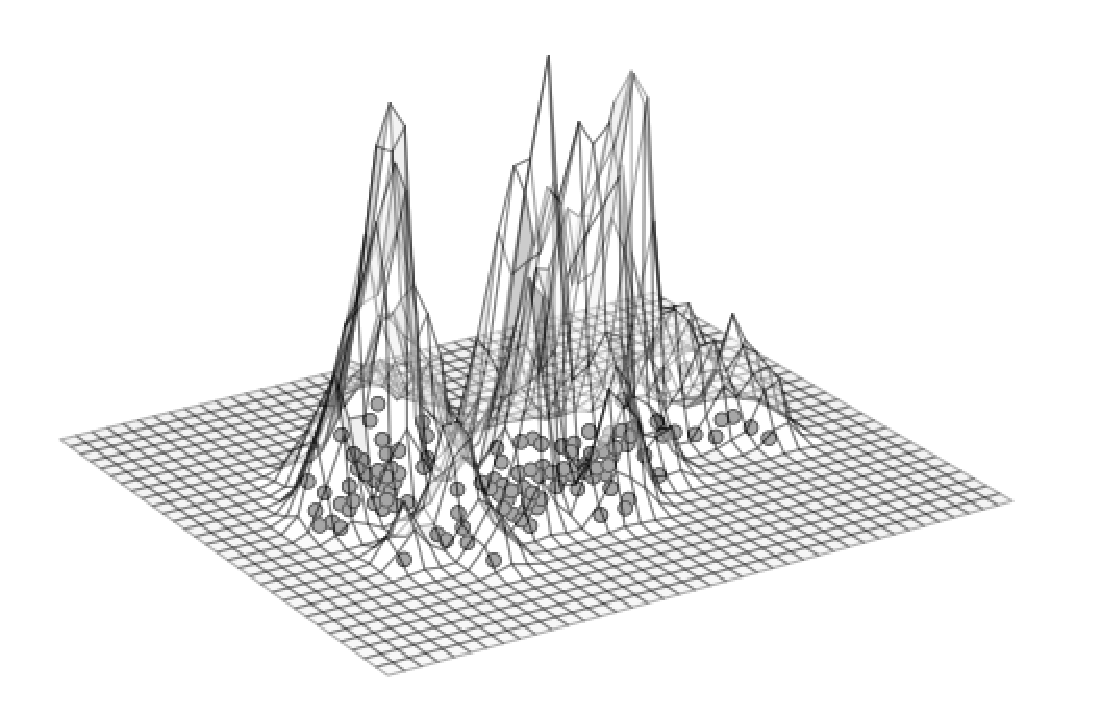
\includegraphics[width=2.5in]{CLUST/density/figs/draftfigs/kde-2d-a}
}{
    \def\scaleF{4}
    \def\myh{0.1}
    \scalebox{0.4}{%
    \begin{pspicture}(2,2)(10,7.5)
	\psPoint(5.9, 3.0, 0.000000){p0}
\psdot(p0)
\psPoint(6.9, 3.1, 0.000000){p1}
\psdot(p1)
\psPoint(6.6, 2.9, 0.000000){p2}
\psdot(p2)
\psPoint(4.6, 3.2, 0.000000){p3}
\psdot(p3)
\psPoint(6.0, 2.2, 0.000000){p4}
\psdot(p4)
\psPoint(4.7, 3.2, 0.000000){p5}
\psdot(p5)
\psPoint(6.5, 3.0, 0.000000){p6}
\psdot(p6)
\psPoint(5.8, 2.7, 0.000000){p7}
\psdot(p7)
\psPoint(6.7, 3.1, 0.000000){p8}
\psdot(p8)
\psPoint(6.7, 2.5, 0.000000){p9}
\psdot(p9)
\psPoint(5.1, 3.7, 0.000000){p10}
\psdot(p10)
\psPoint(5.1, 3.8, 0.000000){p11}
\psdot(p11)
\psPoint(5.7, 3.0, 0.000000){p12}
\psdot(p12)
\psPoint(6.1, 3.0, 0.000000){p13}
\psdot(p13)
\psPoint(4.9, 3.1, 0.000000){p14}
\psdot(p14)
\psPoint(5.0, 3.4, 0.000000){p15}
\psdot(p15)
\psPoint(5.0, 3.4, 0.000000){p16}
\psdot(p16)
\psPoint(5.7, 2.8, 0.000000){p17}
\psdot(p17)
\psPoint(5.0, 3.3, 0.000000){p18}
\psdot(p18)
\psPoint(7.2, 3.2, 0.000000){p19}
\psdot(p19)
\psPoint(5.9, 3.0, 0.000000){p20}
\psdot(p20)
\psPoint(6.5, 3.0, 0.000000){p21}
\psdot(p21)
\psPoint(5.7, 4.4, 0.000000){p22}
\psdot(p22)
\psPoint(5.5, 2.5, 0.000000){p23}
\psdot(p23)
\psPoint(4.9, 2.5, 0.000000){p24}
\psdot(p24)
\psPoint(5.0, 3.5, 0.000000){p25}
\psdot(p25)
\psPoint(5.5, 2.3, 0.000000){p26}
\psdot(p26)
\psPoint(4.6, 3.1, 0.000000){p27}
\psdot(p27)
\psPoint(7.2, 3.0, 0.000000){p28}
\psdot(p28)
\psPoint(6.8, 3.2, 0.000000){p29}
\psdot(p29)
\psPoint(5.4, 3.9, 0.000000){p30}
\psdot(p30)
\psPoint(5.0, 3.2, 0.000000){p31}
\psdot(p31)
\psPoint(5.7, 2.5, 0.000000){p32}
\psdot(p32)
\psPoint(5.8, 2.6, 0.000000){p33}
\psdot(p33)
\psPoint(5.1, 2.5, 0.000000){p34}
\psdot(p34)
\psPoint(5.6, 2.5, 0.000000){p35}
\psdot(p35)
\psPoint(5.8, 2.7, 0.000000){p36}
\psdot(p36)
\psPoint(5.1, 3.8, 0.000000){p37}
\psdot(p37)
\psPoint(6.3, 2.3, 0.000000){p38}
\psdot(p38)
\psPoint(6.3, 2.5, 0.000000){p39}
\psdot(p39)
\psPoint(5.6, 3.0, 0.000000){p40}
\psdot(p40)
\psPoint(6.1, 3.0, 0.000000){p41}
\psdot(p41)
\psPoint(6.8, 3.0, 0.000000){p42}
\psdot(p42)
\psPoint(7.3, 2.9, 0.000000){p43}
\psdot(p43)
\psPoint(5.6, 2.7, 0.000000){p44}
\psdot(p44)
\psPoint(4.8, 3.0, 0.000000){p45}
\psdot(p45)
\psPoint(7.1, 3.0, 0.000000){p46}
\psdot(p46)
\psPoint(5.7, 2.6, 0.000000){p47}
\psdot(p47)
\psPoint(5.3, 3.7, 0.000000){p48}
\psdot(p48)
\psPoint(5.7, 3.8, 0.000000){p49}
\psdot(p49)
\psPoint(5.7, 2.9, 0.000000){p50}
\psdot(p50)
\psPoint(5.6, 2.8, 0.000000){p51}
\psdot(p51)
\psPoint(4.4, 3.0, 0.000000){p52}
\psdot(p52)
\psPoint(6.3, 3.3, 0.000000){p53}
\psdot(p53)
\psPoint(5.4, 3.4, 0.000000){p54}
\psdot(p54)
\psPoint(6.3, 3.4, 0.000000){p55}
\psdot(p55)
\psPoint(6.9, 3.1, 0.000000){p56}
\psdot(p56)
\psPoint(7.7, 3.0, 0.000000){p57}
\psdot(p57)
\psPoint(6.1, 2.8, 0.000000){p58}
\psdot(p58)
\psPoint(5.6, 2.9, 0.000000){p59}
\psdot(p59)
\psPoint(6.1, 2.6, 0.000000){p60}
\psdot(p60)
\psPoint(6.4, 2.7, 0.000000){p61}
\psdot(p61)
\psPoint(5.0, 3.5, 0.000000){p62}
\psdot(p62)
\psPoint(5.1, 3.3, 0.000000){p63}
\psdot(p63)
\psPoint(5.6, 3.0, 0.000000){p64}
\psdot(p64)
\psPoint(5.4, 3.0, 0.000000){p65}
\psdot(p65)
\psPoint(5.8, 2.8, 0.000000){p66}
\psdot(p66)
\psPoint(4.9, 3.1, 0.000000){p67}
\psdot(p67)
\psPoint(4.6, 3.6, 0.000000){p68}
\psdot(p68)
\psPoint(5.2, 3.4, 0.000000){p69}
\psdot(p69)
\psPoint(7.9, 3.8, 0.000000){p70}
\psdot(p70)
\psPoint(7.7, 2.6, 0.000000){p71}
\psdot(p71)
\psPoint(6.1, 2.8, 0.000000){p72}
\psdot(p72)
\psPoint(5.5, 3.5, 0.000000){p73}
\psdot(p73)
\psPoint(4.6, 3.4, 0.000000){p74}
\psdot(p74)
\psPoint(4.7, 3.2, 0.000000){p75}
\psdot(p75)
\psPoint(4.4, 2.9, 0.000000){p76}
\psdot(p76)
\psPoint(6.2, 2.8, 0.000000){p77}
\psdot(p77)
\psPoint(4.8, 3.0, 0.000000){p78}
\psdot(p78)
\psPoint(6.0, 2.9, 0.000000){p79}
\psdot(p79)
\psPoint(6.2, 3.4, 0.000000){p80}
\psdot(p80)
\psPoint(5.0, 2.3, 0.000000){p81}
\psdot(p81)
\psPoint(6.4, 3.2, 0.000000){p82}
\psdot(p82)
\psPoint(6.3, 2.9, 0.000000){p83}
\psdot(p83)
\psPoint(6.7, 3.0, 0.000000){p84}
\psdot(p84)
\psPoint(5.0, 2.0, 0.000000){p85}
\psdot(p85)
\psPoint(5.9, 3.2, 0.000000){p86}
\psdot(p86)
\psPoint(6.7, 3.3, 0.000000){p87}
\psdot(p87)
\psPoint(5.4, 3.9, 0.000000){p88}
\psdot(p88)
\psPoint(6.3, 2.7, 0.000000){p89}
\psdot(p89)
\psPoint(4.8, 3.4, 0.000000){p90}
\psdot(p90)
\psPoint(4.4, 3.2, 0.000000){p91}
\psdot(p91)
\psPoint(6.4, 3.2, 0.000000){p92}
\psdot(p92)
\psPoint(6.2, 2.2, 0.000000){p93}
\psdot(p93)
\psPoint(6.0, 2.2, 0.000000){p94}
\psdot(p94)
\psPoint(7.4, 2.8, 0.000000){p95}
\psdot(p95)
\psPoint(4.9, 2.4, 0.000000){p96}
\psdot(p96)
\psPoint(7.0, 3.2, 0.000000){p97}
\psdot(p97)
\psPoint(5.5, 2.4, 0.000000){p98}
\psdot(p98)
\psPoint(6.3, 3.3, 0.000000){p99}
\psdot(p99)
\psPoint(6.8, 2.8, 0.000000){p100}
\psdot(p100)
\psPoint(6.1, 2.9, 0.000000){p101}
\psdot(p101)
\psPoint(6.5, 3.2, 0.000000){p102}
\psdot(p102)
\psPoint(6.7, 3.3, 0.000000){p103}
\psdot(p103)
\psPoint(6.7, 3.1, 0.000000){p104}
\psdot(p104)
\psPoint(4.8, 3.4, 0.000000){p105}
\psdot(p105)
\psPoint(4.9, 3.0, 0.000000){p106}
\psdot(p106)
\psPoint(6.9, 3.2, 0.000000){p107}
\psdot(p107)
\psPoint(4.5, 2.3, 0.000000){p108}
\psdot(p108)
\psPoint(4.3, 3.0, 0.000000){p109}
\psdot(p109)
\psPoint(5.2, 2.7, 0.000000){p110}
\psdot(p110)
\psPoint(5.0, 3.6, 0.000000){p111}
\psdot(p111)
\psPoint(6.4, 2.9, 0.000000){p112}
\psdot(p112)
\psPoint(5.2, 3.5, 0.000000){p113}
\psdot(p113)
\psPoint(5.8, 2.7, 0.000000){p114}
\psdot(p114)
\psPoint(5.5, 4.2, 0.000000){p115}
\psdot(p115)
\psPoint(7.6, 3.0, 0.000000){p116}
\psdot(p116)
\psPoint(6.3, 2.8, 0.000000){p117}
\psdot(p117)
\psPoint(6.4, 3.1, 0.000000){p118}
\psdot(p118)
\psPoint(6.3, 2.5, 0.000000){p119}
\psdot(p119)
\psPoint(5.8, 2.7, 0.000000){p120}
\psdot(p120)
\psPoint(5.0, 3.0, 0.000000){p121}
\psdot(p121)
\psPoint(6.7, 3.1, 0.000000){p122}
\psdot(p122)
\psPoint(6.0, 2.7, 0.000000){p123}
\psdot(p123)
\psPoint(5.1, 3.5, 0.000000){p124}
\psdot(p124)
\psPoint(4.8, 3.1, 0.000000){p125}
\psdot(p125)
\psPoint(5.7, 2.8, 0.000000){p126}
\psdot(p126)
\psPoint(5.1, 3.8, 0.000000){p127}
\psdot(p127)
\psPoint(6.6, 3.0, 0.000000){p128}
\psdot(p128)
\psPoint(6.4, 2.8, 0.000000){p129}
\psdot(p129)
\psPoint(5.2, 4.1, 0.000000){p130}
\psdot(p130)
\psPoint(6.4, 2.8, 0.000000){p131}
\psdot(p131)
\psPoint(7.7, 2.8, 0.000000){p132}
\psdot(p132)
\psPoint(5.8, 4.0, 0.000000){p133}
\psdot(p133)
\psPoint(4.9, 3.1, 0.000000){p134}
\psdot(p134)
\psPoint(5.4, 3.7, 0.000000){p135}
\psdot(p135)
\psPoint(5.1, 3.5, 0.000000){p136}
\psdot(p136)
\psPoint(6.0, 3.4, 0.000000){p137}
\psdot(p137)
\psPoint(6.5, 3.0, 0.000000){p138}
\psdot(p138)
\psPoint(5.5, 2.4, 0.000000){p139}
\psdot(p139)
\psPoint(7.2, 3.6, 0.000000){p140}
\psdot(p140)
\psPoint(6.9, 3.1, 0.000000){p141}
\psdot(p141)
\psPoint(6.2, 2.9, 0.000000){p142}
\psdot(p142)
\psPoint(6.5, 2.8, 0.000000){p143}
\psdot(p143)
\psPoint(6.0, 3.0, 0.000000){p144}
\psdot(p144)
\psPoint(5.4, 3.4, 0.000000){p145}
\psdot(p145)
\psPoint(5.5, 2.6, 0.000000){p146}
\psdot(p146)
\psPoint(6.7, 3.0, 0.000000){p147}
\psdot(p147)
\psPoint(7.7, 3.8, 0.000000){p148}
\psdot(p148)
\psPoint(5.1, 3.4, 0.000000){p149}
\psdot(p149)

	\psset{fillcolor=white}
	\psSurface[ngrid=40 30,	algebraic](3.5,1)(8.5,5){%
\scaleF*(0.001061/\myh^2)*
(e^((-0.5/\myh^2)*((x-5.90)^2 + (y-3.00)^2))+
e^((-0.5/\myh^2)*((x-6.90)^2 + (y-3.10)^2))+
e^((-0.5/\myh^2)*((x-6.60)^2 + (y-2.90)^2))+
e^((-0.5/\myh^2)*((x-4.60)^2 + (y-3.20)^2))+
e^((-0.5/\myh^2)*((x-6.00)^2 + (y-2.20)^2))+
e^((-0.5/\myh^2)*((x-4.70)^2 + (y-3.20)^2))+
e^((-0.5/\myh^2)*((x-6.50)^2 + (y-3.00)^2))+
e^((-0.5/\myh^2)*((x-5.80)^2 + (y-2.70)^2))+
e^((-0.5/\myh^2)*((x-6.70)^2 + (y-3.10)^2))+
e^((-0.5/\myh^2)*((x-6.70)^2 + (y-2.50)^2))+
e^((-0.5/\myh^2)*((x-5.10)^2 + (y-3.70)^2))+
e^((-0.5/\myh^2)*((x-5.10)^2 + (y-3.80)^2))+
e^((-0.5/\myh^2)*((x-5.70)^2 + (y-3.00)^2))+
e^((-0.5/\myh^2)*((x-6.10)^2 + (y-3.00)^2))+
e^((-0.5/\myh^2)*((x-4.90)^2 + (y-3.10)^2))+
e^((-0.5/\myh^2)*((x-5.00)^2 + (y-3.40)^2))+
e^((-0.5/\myh^2)*((x-5.00)^2 + (y-3.40)^2))+
e^((-0.5/\myh^2)*((x-5.70)^2 + (y-2.80)^2))+
e^((-0.5/\myh^2)*((x-5.00)^2 + (y-3.30)^2))+
e^((-0.5/\myh^2)*((x-7.20)^2 + (y-3.20)^2))+
e^((-0.5/\myh^2)*((x-5.90)^2 + (y-3.00)^2))+
e^((-0.5/\myh^2)*((x-6.50)^2 + (y-3.00)^2))+
e^((-0.5/\myh^2)*((x-5.70)^2 + (y-4.40)^2))+
e^((-0.5/\myh^2)*((x-5.50)^2 + (y-2.50)^2))+
e^((-0.5/\myh^2)*((x-4.90)^2 + (y-2.50)^2))+
e^((-0.5/\myh^2)*((x-5.00)^2 + (y-3.50)^2))+
e^((-0.5/\myh^2)*((x-5.50)^2 + (y-2.30)^2))+
e^((-0.5/\myh^2)*((x-4.60)^2 + (y-3.10)^2))+
e^((-0.5/\myh^2)*((x-7.20)^2 + (y-3.00)^2))+
e^((-0.5/\myh^2)*((x-6.80)^2 + (y-3.20)^2))+
e^((-0.5/\myh^2)*((x-5.40)^2 + (y-3.90)^2))+
e^((-0.5/\myh^2)*((x-5.00)^2 + (y-3.20)^2))+
e^((-0.5/\myh^2)*((x-5.70)^2 + (y-2.50)^2))+
e^((-0.5/\myh^2)*((x-5.80)^2 + (y-2.60)^2))+
e^((-0.5/\myh^2)*((x-5.10)^2 + (y-2.50)^2))+
e^((-0.5/\myh^2)*((x-5.60)^2 + (y-2.50)^2))+
e^((-0.5/\myh^2)*((x-5.80)^2 + (y-2.70)^2))+
e^((-0.5/\myh^2)*((x-5.10)^2 + (y-3.80)^2))+
e^((-0.5/\myh^2)*((x-6.30)^2 + (y-2.30)^2))+
e^((-0.5/\myh^2)*((x-6.30)^2 + (y-2.50)^2))+
e^((-0.5/\myh^2)*((x-5.60)^2 + (y-3.00)^2))+
e^((-0.5/\myh^2)*((x-6.10)^2 + (y-3.00)^2))+
e^((-0.5/\myh^2)*((x-6.80)^2 + (y-3.00)^2))+
e^((-0.5/\myh^2)*((x-7.30)^2 + (y-2.90)^2))+
e^((-0.5/\myh^2)*((x-5.60)^2 + (y-2.70)^2))+
e^((-0.5/\myh^2)*((x-4.80)^2 + (y-3.00)^2))+
e^((-0.5/\myh^2)*((x-7.10)^2 + (y-3.00)^2))+
e^((-0.5/\myh^2)*((x-5.70)^2 + (y-2.60)^2))+
e^((-0.5/\myh^2)*((x-5.30)^2 + (y-3.70)^2))+
e^((-0.5/\myh^2)*((x-5.70)^2 + (y-3.80)^2))+
e^((-0.5/\myh^2)*((x-5.70)^2 + (y-2.90)^2))+
e^((-0.5/\myh^2)*((x-5.60)^2 + (y-2.80)^2))+
e^((-0.5/\myh^2)*((x-4.40)^2 + (y-3.00)^2))+
e^((-0.5/\myh^2)*((x-6.30)^2 + (y-3.30)^2))+
e^((-0.5/\myh^2)*((x-5.40)^2 + (y-3.40)^2))+
e^((-0.5/\myh^2)*((x-6.30)^2 + (y-3.40)^2))+
e^((-0.5/\myh^2)*((x-6.90)^2 + (y-3.10)^2))+
e^((-0.5/\myh^2)*((x-7.70)^2 + (y-3.00)^2))+
e^((-0.5/\myh^2)*((x-6.10)^2 + (y-2.80)^2))+
e^((-0.5/\myh^2)*((x-5.60)^2 + (y-2.90)^2))+
e^((-0.5/\myh^2)*((x-6.10)^2 + (y-2.60)^2))+
e^((-0.5/\myh^2)*((x-6.40)^2 + (y-2.70)^2))+
e^((-0.5/\myh^2)*((x-5.00)^2 + (y-3.50)^2))+
e^((-0.5/\myh^2)*((x-5.10)^2 + (y-3.30)^2))+
e^((-0.5/\myh^2)*((x-5.60)^2 + (y-3.00)^2))+
e^((-0.5/\myh^2)*((x-5.40)^2 + (y-3.00)^2))+
e^((-0.5/\myh^2)*((x-5.80)^2 + (y-2.80)^2))+
e^((-0.5/\myh^2)*((x-4.90)^2 + (y-3.10)^2))+
e^((-0.5/\myh^2)*((x-4.60)^2 + (y-3.60)^2))+
e^((-0.5/\myh^2)*((x-5.20)^2 + (y-3.40)^2))+
e^((-0.5/\myh^2)*((x-7.90)^2 + (y-3.80)^2))+
e^((-0.5/\myh^2)*((x-7.70)^2 + (y-2.60)^2))+
e^((-0.5/\myh^2)*((x-6.10)^2 + (y-2.80)^2))+
e^((-0.5/\myh^2)*((x-5.50)^2 + (y-3.50)^2))+
e^((-0.5/\myh^2)*((x-4.60)^2 + (y-3.40)^2))+
e^((-0.5/\myh^2)*((x-4.70)^2 + (y-3.20)^2))+
e^((-0.5/\myh^2)*((x-4.40)^2 + (y-2.90)^2))+
e^((-0.5/\myh^2)*((x-6.20)^2 + (y-2.80)^2))+
e^((-0.5/\myh^2)*((x-4.80)^2 + (y-3.00)^2))+
e^((-0.5/\myh^2)*((x-6.00)^2 + (y-2.90)^2))+
e^((-0.5/\myh^2)*((x-6.20)^2 + (y-3.40)^2))+
e^((-0.5/\myh^2)*((x-5.00)^2 + (y-2.30)^2))+
e^((-0.5/\myh^2)*((x-6.40)^2 + (y-3.20)^2))+
e^((-0.5/\myh^2)*((x-6.30)^2 + (y-2.90)^2))+
e^((-0.5/\myh^2)*((x-6.70)^2 + (y-3.00)^2))+
e^((-0.5/\myh^2)*((x-5.00)^2 + (y-2.00)^2))+
e^((-0.5/\myh^2)*((x-5.90)^2 + (y-3.20)^2))+
e^((-0.5/\myh^2)*((x-6.70)^2 + (y-3.30)^2))+
e^((-0.5/\myh^2)*((x-5.40)^2 + (y-3.90)^2))+
e^((-0.5/\myh^2)*((x-6.30)^2 + (y-2.70)^2))+
e^((-0.5/\myh^2)*((x-4.80)^2 + (y-3.40)^2))+
e^((-0.5/\myh^2)*((x-4.40)^2 + (y-3.20)^2))+
e^((-0.5/\myh^2)*((x-6.40)^2 + (y-3.20)^2))+
e^((-0.5/\myh^2)*((x-6.20)^2 + (y-2.20)^2))+
e^((-0.5/\myh^2)*((x-6.00)^2 + (y-2.20)^2))+
e^((-0.5/\myh^2)*((x-7.40)^2 + (y-2.80)^2))+
e^((-0.5/\myh^2)*((x-4.90)^2 + (y-2.40)^2))+
e^((-0.5/\myh^2)*((x-7.00)^2 + (y-3.20)^2))+
e^((-0.5/\myh^2)*((x-5.50)^2 + (y-2.40)^2))+
e^((-0.5/\myh^2)*((x-6.30)^2 + (y-3.30)^2))+
e^((-0.5/\myh^2)*((x-6.80)^2 + (y-2.80)^2))+
e^((-0.5/\myh^2)*((x-6.10)^2 + (y-2.90)^2))+
e^((-0.5/\myh^2)*((x-6.50)^2 + (y-3.20)^2))+
e^((-0.5/\myh^2)*((x-6.70)^2 + (y-3.30)^2))+
e^((-0.5/\myh^2)*((x-6.70)^2 + (y-3.10)^2))+
e^((-0.5/\myh^2)*((x-4.80)^2 + (y-3.40)^2))+
e^((-0.5/\myh^2)*((x-4.90)^2 + (y-3.00)^2))+
e^((-0.5/\myh^2)*((x-6.90)^2 + (y-3.20)^2))+
e^((-0.5/\myh^2)*((x-4.50)^2 + (y-2.30)^2))+
e^((-0.5/\myh^2)*((x-4.30)^2 + (y-3.00)^2))+
e^((-0.5/\myh^2)*((x-5.20)^2 + (y-2.70)^2))+
e^((-0.5/\myh^2)*((x-5.00)^2 + (y-3.60)^2))+
e^((-0.5/\myh^2)*((x-6.40)^2 + (y-2.90)^2))+
e^((-0.5/\myh^2)*((x-5.20)^2 + (y-3.50)^2))+
e^((-0.5/\myh^2)*((x-5.80)^2 + (y-2.70)^2))+
e^((-0.5/\myh^2)*((x-5.50)^2 + (y-4.20)^2))+
e^((-0.5/\myh^2)*((x-7.60)^2 + (y-3.00)^2))+
e^((-0.5/\myh^2)*((x-6.30)^2 + (y-2.80)^2))+
e^((-0.5/\myh^2)*((x-6.40)^2 + (y-3.10)^2))+
e^((-0.5/\myh^2)*((x-6.30)^2 + (y-2.50)^2))+
e^((-0.5/\myh^2)*((x-5.80)^2 + (y-2.70)^2))+
e^((-0.5/\myh^2)*((x-5.00)^2 + (y-3.00)^2))+
e^((-0.5/\myh^2)*((x-6.70)^2 + (y-3.10)^2))+
e^((-0.5/\myh^2)*((x-6.00)^2 + (y-2.70)^2))+
e^((-0.5/\myh^2)*((x-5.10)^2 + (y-3.50)^2))+
e^((-0.5/\myh^2)*((x-4.80)^2 + (y-3.10)^2))+
e^((-0.5/\myh^2)*((x-5.70)^2 + (y-2.80)^2))+
e^((-0.5/\myh^2)*((x-5.10)^2 + (y-3.80)^2))+
e^((-0.5/\myh^2)*((x-6.60)^2 + (y-3.00)^2))+
e^((-0.5/\myh^2)*((x-6.40)^2 + (y-2.80)^2))+
e^((-0.5/\myh^2)*((x-5.20)^2 + (y-4.10)^2))+
e^((-0.5/\myh^2)*((x-6.40)^2 + (y-2.80)^2))+
e^((-0.5/\myh^2)*((x-7.70)^2 + (y-2.80)^2))+
e^((-0.5/\myh^2)*((x-5.80)^2 + (y-4.00)^2))+
e^((-0.5/\myh^2)*((x-4.90)^2 + (y-3.10)^2))+
e^((-0.5/\myh^2)*((x-5.40)^2 + (y-3.70)^2))+
e^((-0.5/\myh^2)*((x-5.10)^2 + (y-3.50)^2))+
e^((-0.5/\myh^2)*((x-6.00)^2 + (y-3.40)^2))+
e^((-0.5/\myh^2)*((x-6.50)^2 + (y-3.00)^2))+
e^((-0.5/\myh^2)*((x-5.50)^2 + (y-2.40)^2))+
e^((-0.5/\myh^2)*((x-7.20)^2 + (y-3.60)^2))+
e^((-0.5/\myh^2)*((x-6.90)^2 + (y-3.10)^2))+
e^((-0.5/\myh^2)*((x-6.20)^2 + (y-2.90)^2))+
e^((-0.5/\myh^2)*((x-6.50)^2 + (y-2.80)^2))+
e^((-0.5/\myh^2)*((x-6.00)^2 + (y-3.00)^2))+
e^((-0.5/\myh^2)*((x-5.40)^2 + (y-3.40)^2))+
e^((-0.5/\myh^2)*((x-5.50)^2 + (y-2.60)^2))+
e^((-0.5/\myh^2)*((x-6.70)^2 + (y-3.00)^2))+
e^((-0.5/\myh^2)*((x-7.70)^2 + (y-3.80)^2))+
e^((-0.5/\myh^2)*((x-5.10)^2 + (y-3.40)^2)))
}
\end{pspicture}


    }
    }}
\vspace{0.1in}
\subfloat[$h=0.2$]{
\label{fig:clust:den:kde2dGb}
\ifdraft{
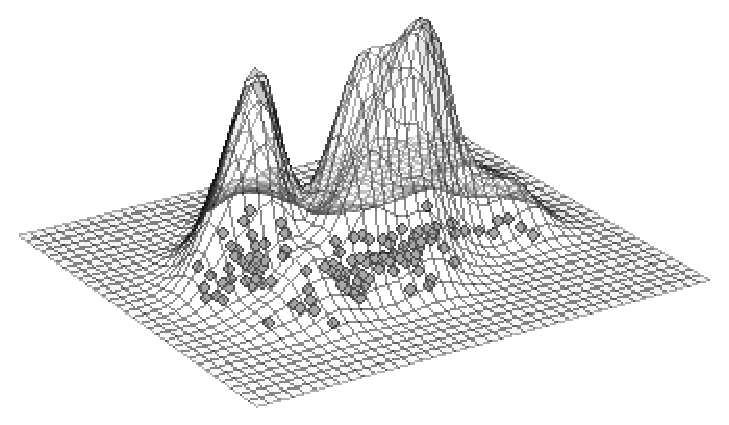
\includegraphics[width=2.5in]{CLUST/density/figs/draftfigs/kde-2d-b}
}{
    \def\scaleF{5}
    \def\myh{0.2}
    \scalebox{0.4}{%
    \begin{pspicture}(2,2)(10,7.5)
	\psPoint(5.9, 3.0, 0.000000){p0}
\psdot(p0)
\psPoint(6.9, 3.1, 0.000000){p1}
\psdot(p1)
\psPoint(6.6, 2.9, 0.000000){p2}
\psdot(p2)
\psPoint(4.6, 3.2, 0.000000){p3}
\psdot(p3)
\psPoint(6.0, 2.2, 0.000000){p4}
\psdot(p4)
\psPoint(4.7, 3.2, 0.000000){p5}
\psdot(p5)
\psPoint(6.5, 3.0, 0.000000){p6}
\psdot(p6)
\psPoint(5.8, 2.7, 0.000000){p7}
\psdot(p7)
\psPoint(6.7, 3.1, 0.000000){p8}
\psdot(p8)
\psPoint(6.7, 2.5, 0.000000){p9}
\psdot(p9)
\psPoint(5.1, 3.7, 0.000000){p10}
\psdot(p10)
\psPoint(5.1, 3.8, 0.000000){p11}
\psdot(p11)
\psPoint(5.7, 3.0, 0.000000){p12}
\psdot(p12)
\psPoint(6.1, 3.0, 0.000000){p13}
\psdot(p13)
\psPoint(4.9, 3.1, 0.000000){p14}
\psdot(p14)
\psPoint(5.0, 3.4, 0.000000){p15}
\psdot(p15)
\psPoint(5.0, 3.4, 0.000000){p16}
\psdot(p16)
\psPoint(5.7, 2.8, 0.000000){p17}
\psdot(p17)
\psPoint(5.0, 3.3, 0.000000){p18}
\psdot(p18)
\psPoint(7.2, 3.2, 0.000000){p19}
\psdot(p19)
\psPoint(5.9, 3.0, 0.000000){p20}
\psdot(p20)
\psPoint(6.5, 3.0, 0.000000){p21}
\psdot(p21)
\psPoint(5.7, 4.4, 0.000000){p22}
\psdot(p22)
\psPoint(5.5, 2.5, 0.000000){p23}
\psdot(p23)
\psPoint(4.9, 2.5, 0.000000){p24}
\psdot(p24)
\psPoint(5.0, 3.5, 0.000000){p25}
\psdot(p25)
\psPoint(5.5, 2.3, 0.000000){p26}
\psdot(p26)
\psPoint(4.6, 3.1, 0.000000){p27}
\psdot(p27)
\psPoint(7.2, 3.0, 0.000000){p28}
\psdot(p28)
\psPoint(6.8, 3.2, 0.000000){p29}
\psdot(p29)
\psPoint(5.4, 3.9, 0.000000){p30}
\psdot(p30)
\psPoint(5.0, 3.2, 0.000000){p31}
\psdot(p31)
\psPoint(5.7, 2.5, 0.000000){p32}
\psdot(p32)
\psPoint(5.8, 2.6, 0.000000){p33}
\psdot(p33)
\psPoint(5.1, 2.5, 0.000000){p34}
\psdot(p34)
\psPoint(5.6, 2.5, 0.000000){p35}
\psdot(p35)
\psPoint(5.8, 2.7, 0.000000){p36}
\psdot(p36)
\psPoint(5.1, 3.8, 0.000000){p37}
\psdot(p37)
\psPoint(6.3, 2.3, 0.000000){p38}
\psdot(p38)
\psPoint(6.3, 2.5, 0.000000){p39}
\psdot(p39)
\psPoint(5.6, 3.0, 0.000000){p40}
\psdot(p40)
\psPoint(6.1, 3.0, 0.000000){p41}
\psdot(p41)
\psPoint(6.8, 3.0, 0.000000){p42}
\psdot(p42)
\psPoint(7.3, 2.9, 0.000000){p43}
\psdot(p43)
\psPoint(5.6, 2.7, 0.000000){p44}
\psdot(p44)
\psPoint(4.8, 3.0, 0.000000){p45}
\psdot(p45)
\psPoint(7.1, 3.0, 0.000000){p46}
\psdot(p46)
\psPoint(5.7, 2.6, 0.000000){p47}
\psdot(p47)
\psPoint(5.3, 3.7, 0.000000){p48}
\psdot(p48)
\psPoint(5.7, 3.8, 0.000000){p49}
\psdot(p49)
\psPoint(5.7, 2.9, 0.000000){p50}
\psdot(p50)
\psPoint(5.6, 2.8, 0.000000){p51}
\psdot(p51)
\psPoint(4.4, 3.0, 0.000000){p52}
\psdot(p52)
\psPoint(6.3, 3.3, 0.000000){p53}
\psdot(p53)
\psPoint(5.4, 3.4, 0.000000){p54}
\psdot(p54)
\psPoint(6.3, 3.4, 0.000000){p55}
\psdot(p55)
\psPoint(6.9, 3.1, 0.000000){p56}
\psdot(p56)
\psPoint(7.7, 3.0, 0.000000){p57}
\psdot(p57)
\psPoint(6.1, 2.8, 0.000000){p58}
\psdot(p58)
\psPoint(5.6, 2.9, 0.000000){p59}
\psdot(p59)
\psPoint(6.1, 2.6, 0.000000){p60}
\psdot(p60)
\psPoint(6.4, 2.7, 0.000000){p61}
\psdot(p61)
\psPoint(5.0, 3.5, 0.000000){p62}
\psdot(p62)
\psPoint(5.1, 3.3, 0.000000){p63}
\psdot(p63)
\psPoint(5.6, 3.0, 0.000000){p64}
\psdot(p64)
\psPoint(5.4, 3.0, 0.000000){p65}
\psdot(p65)
\psPoint(5.8, 2.8, 0.000000){p66}
\psdot(p66)
\psPoint(4.9, 3.1, 0.000000){p67}
\psdot(p67)
\psPoint(4.6, 3.6, 0.000000){p68}
\psdot(p68)
\psPoint(5.2, 3.4, 0.000000){p69}
\psdot(p69)
\psPoint(7.9, 3.8, 0.000000){p70}
\psdot(p70)
\psPoint(7.7, 2.6, 0.000000){p71}
\psdot(p71)
\psPoint(6.1, 2.8, 0.000000){p72}
\psdot(p72)
\psPoint(5.5, 3.5, 0.000000){p73}
\psdot(p73)
\psPoint(4.6, 3.4, 0.000000){p74}
\psdot(p74)
\psPoint(4.7, 3.2, 0.000000){p75}
\psdot(p75)
\psPoint(4.4, 2.9, 0.000000){p76}
\psdot(p76)
\psPoint(6.2, 2.8, 0.000000){p77}
\psdot(p77)
\psPoint(4.8, 3.0, 0.000000){p78}
\psdot(p78)
\psPoint(6.0, 2.9, 0.000000){p79}
\psdot(p79)
\psPoint(6.2, 3.4, 0.000000){p80}
\psdot(p80)
\psPoint(5.0, 2.3, 0.000000){p81}
\psdot(p81)
\psPoint(6.4, 3.2, 0.000000){p82}
\psdot(p82)
\psPoint(6.3, 2.9, 0.000000){p83}
\psdot(p83)
\psPoint(6.7, 3.0, 0.000000){p84}
\psdot(p84)
\psPoint(5.0, 2.0, 0.000000){p85}
\psdot(p85)
\psPoint(5.9, 3.2, 0.000000){p86}
\psdot(p86)
\psPoint(6.7, 3.3, 0.000000){p87}
\psdot(p87)
\psPoint(5.4, 3.9, 0.000000){p88}
\psdot(p88)
\psPoint(6.3, 2.7, 0.000000){p89}
\psdot(p89)
\psPoint(4.8, 3.4, 0.000000){p90}
\psdot(p90)
\psPoint(4.4, 3.2, 0.000000){p91}
\psdot(p91)
\psPoint(6.4, 3.2, 0.000000){p92}
\psdot(p92)
\psPoint(6.2, 2.2, 0.000000){p93}
\psdot(p93)
\psPoint(6.0, 2.2, 0.000000){p94}
\psdot(p94)
\psPoint(7.4, 2.8, 0.000000){p95}
\psdot(p95)
\psPoint(4.9, 2.4, 0.000000){p96}
\psdot(p96)
\psPoint(7.0, 3.2, 0.000000){p97}
\psdot(p97)
\psPoint(5.5, 2.4, 0.000000){p98}
\psdot(p98)
\psPoint(6.3, 3.3, 0.000000){p99}
\psdot(p99)
\psPoint(6.8, 2.8, 0.000000){p100}
\psdot(p100)
\psPoint(6.1, 2.9, 0.000000){p101}
\psdot(p101)
\psPoint(6.5, 3.2, 0.000000){p102}
\psdot(p102)
\psPoint(6.7, 3.3, 0.000000){p103}
\psdot(p103)
\psPoint(6.7, 3.1, 0.000000){p104}
\psdot(p104)
\psPoint(4.8, 3.4, 0.000000){p105}
\psdot(p105)
\psPoint(4.9, 3.0, 0.000000){p106}
\psdot(p106)
\psPoint(6.9, 3.2, 0.000000){p107}
\psdot(p107)
\psPoint(4.5, 2.3, 0.000000){p108}
\psdot(p108)
\psPoint(4.3, 3.0, 0.000000){p109}
\psdot(p109)
\psPoint(5.2, 2.7, 0.000000){p110}
\psdot(p110)
\psPoint(5.0, 3.6, 0.000000){p111}
\psdot(p111)
\psPoint(6.4, 2.9, 0.000000){p112}
\psdot(p112)
\psPoint(5.2, 3.5, 0.000000){p113}
\psdot(p113)
\psPoint(5.8, 2.7, 0.000000){p114}
\psdot(p114)
\psPoint(5.5, 4.2, 0.000000){p115}
\psdot(p115)
\psPoint(7.6, 3.0, 0.000000){p116}
\psdot(p116)
\psPoint(6.3, 2.8, 0.000000){p117}
\psdot(p117)
\psPoint(6.4, 3.1, 0.000000){p118}
\psdot(p118)
\psPoint(6.3, 2.5, 0.000000){p119}
\psdot(p119)
\psPoint(5.8, 2.7, 0.000000){p120}
\psdot(p120)
\psPoint(5.0, 3.0, 0.000000){p121}
\psdot(p121)
\psPoint(6.7, 3.1, 0.000000){p122}
\psdot(p122)
\psPoint(6.0, 2.7, 0.000000){p123}
\psdot(p123)
\psPoint(5.1, 3.5, 0.000000){p124}
\psdot(p124)
\psPoint(4.8, 3.1, 0.000000){p125}
\psdot(p125)
\psPoint(5.7, 2.8, 0.000000){p126}
\psdot(p126)
\psPoint(5.1, 3.8, 0.000000){p127}
\psdot(p127)
\psPoint(6.6, 3.0, 0.000000){p128}
\psdot(p128)
\psPoint(6.4, 2.8, 0.000000){p129}
\psdot(p129)
\psPoint(5.2, 4.1, 0.000000){p130}
\psdot(p130)
\psPoint(6.4, 2.8, 0.000000){p131}
\psdot(p131)
\psPoint(7.7, 2.8, 0.000000){p132}
\psdot(p132)
\psPoint(5.8, 4.0, 0.000000){p133}
\psdot(p133)
\psPoint(4.9, 3.1, 0.000000){p134}
\psdot(p134)
\psPoint(5.4, 3.7, 0.000000){p135}
\psdot(p135)
\psPoint(5.1, 3.5, 0.000000){p136}
\psdot(p136)
\psPoint(6.0, 3.4, 0.000000){p137}
\psdot(p137)
\psPoint(6.5, 3.0, 0.000000){p138}
\psdot(p138)
\psPoint(5.5, 2.4, 0.000000){p139}
\psdot(p139)
\psPoint(7.2, 3.6, 0.000000){p140}
\psdot(p140)
\psPoint(6.9, 3.1, 0.000000){p141}
\psdot(p141)
\psPoint(6.2, 2.9, 0.000000){p142}
\psdot(p142)
\psPoint(6.5, 2.8, 0.000000){p143}
\psdot(p143)
\psPoint(6.0, 3.0, 0.000000){p144}
\psdot(p144)
\psPoint(5.4, 3.4, 0.000000){p145}
\psdot(p145)
\psPoint(5.5, 2.6, 0.000000){p146}
\psdot(p146)
\psPoint(6.7, 3.0, 0.000000){p147}
\psdot(p147)
\psPoint(7.7, 3.8, 0.000000){p148}
\psdot(p148)
\psPoint(5.1, 3.4, 0.000000){p149}
\psdot(p149)

	\psset{fillcolor=white}
	\psSurface[ngrid=40 30,	algebraic](3.5,1)(8.5,5){%
\scaleF*(0.001061/\myh^2)*
(e^((-0.5/\myh^2)*((x-5.90)^2 + (y-3.00)^2))+
e^((-0.5/\myh^2)*((x-6.90)^2 + (y-3.10)^2))+
e^((-0.5/\myh^2)*((x-6.60)^2 + (y-2.90)^2))+
e^((-0.5/\myh^2)*((x-4.60)^2 + (y-3.20)^2))+
e^((-0.5/\myh^2)*((x-6.00)^2 + (y-2.20)^2))+
e^((-0.5/\myh^2)*((x-4.70)^2 + (y-3.20)^2))+
e^((-0.5/\myh^2)*((x-6.50)^2 + (y-3.00)^2))+
e^((-0.5/\myh^2)*((x-5.80)^2 + (y-2.70)^2))+
e^((-0.5/\myh^2)*((x-6.70)^2 + (y-3.10)^2))+
e^((-0.5/\myh^2)*((x-6.70)^2 + (y-2.50)^2))+
e^((-0.5/\myh^2)*((x-5.10)^2 + (y-3.70)^2))+
e^((-0.5/\myh^2)*((x-5.10)^2 + (y-3.80)^2))+
e^((-0.5/\myh^2)*((x-5.70)^2 + (y-3.00)^2))+
e^((-0.5/\myh^2)*((x-6.10)^2 + (y-3.00)^2))+
e^((-0.5/\myh^2)*((x-4.90)^2 + (y-3.10)^2))+
e^((-0.5/\myh^2)*((x-5.00)^2 + (y-3.40)^2))+
e^((-0.5/\myh^2)*((x-5.00)^2 + (y-3.40)^2))+
e^((-0.5/\myh^2)*((x-5.70)^2 + (y-2.80)^2))+
e^((-0.5/\myh^2)*((x-5.00)^2 + (y-3.30)^2))+
e^((-0.5/\myh^2)*((x-7.20)^2 + (y-3.20)^2))+
e^((-0.5/\myh^2)*((x-5.90)^2 + (y-3.00)^2))+
e^((-0.5/\myh^2)*((x-6.50)^2 + (y-3.00)^2))+
e^((-0.5/\myh^2)*((x-5.70)^2 + (y-4.40)^2))+
e^((-0.5/\myh^2)*((x-5.50)^2 + (y-2.50)^2))+
e^((-0.5/\myh^2)*((x-4.90)^2 + (y-2.50)^2))+
e^((-0.5/\myh^2)*((x-5.00)^2 + (y-3.50)^2))+
e^((-0.5/\myh^2)*((x-5.50)^2 + (y-2.30)^2))+
e^((-0.5/\myh^2)*((x-4.60)^2 + (y-3.10)^2))+
e^((-0.5/\myh^2)*((x-7.20)^2 + (y-3.00)^2))+
e^((-0.5/\myh^2)*((x-6.80)^2 + (y-3.20)^2))+
e^((-0.5/\myh^2)*((x-5.40)^2 + (y-3.90)^2))+
e^((-0.5/\myh^2)*((x-5.00)^2 + (y-3.20)^2))+
e^((-0.5/\myh^2)*((x-5.70)^2 + (y-2.50)^2))+
e^((-0.5/\myh^2)*((x-5.80)^2 + (y-2.60)^2))+
e^((-0.5/\myh^2)*((x-5.10)^2 + (y-2.50)^2))+
e^((-0.5/\myh^2)*((x-5.60)^2 + (y-2.50)^2))+
e^((-0.5/\myh^2)*((x-5.80)^2 + (y-2.70)^2))+
e^((-0.5/\myh^2)*((x-5.10)^2 + (y-3.80)^2))+
e^((-0.5/\myh^2)*((x-6.30)^2 + (y-2.30)^2))+
e^((-0.5/\myh^2)*((x-6.30)^2 + (y-2.50)^2))+
e^((-0.5/\myh^2)*((x-5.60)^2 + (y-3.00)^2))+
e^((-0.5/\myh^2)*((x-6.10)^2 + (y-3.00)^2))+
e^((-0.5/\myh^2)*((x-6.80)^2 + (y-3.00)^2))+
e^((-0.5/\myh^2)*((x-7.30)^2 + (y-2.90)^2))+
e^((-0.5/\myh^2)*((x-5.60)^2 + (y-2.70)^2))+
e^((-0.5/\myh^2)*((x-4.80)^2 + (y-3.00)^2))+
e^((-0.5/\myh^2)*((x-7.10)^2 + (y-3.00)^2))+
e^((-0.5/\myh^2)*((x-5.70)^2 + (y-2.60)^2))+
e^((-0.5/\myh^2)*((x-5.30)^2 + (y-3.70)^2))+
e^((-0.5/\myh^2)*((x-5.70)^2 + (y-3.80)^2))+
e^((-0.5/\myh^2)*((x-5.70)^2 + (y-2.90)^2))+
e^((-0.5/\myh^2)*((x-5.60)^2 + (y-2.80)^2))+
e^((-0.5/\myh^2)*((x-4.40)^2 + (y-3.00)^2))+
e^((-0.5/\myh^2)*((x-6.30)^2 + (y-3.30)^2))+
e^((-0.5/\myh^2)*((x-5.40)^2 + (y-3.40)^2))+
e^((-0.5/\myh^2)*((x-6.30)^2 + (y-3.40)^2))+
e^((-0.5/\myh^2)*((x-6.90)^2 + (y-3.10)^2))+
e^((-0.5/\myh^2)*((x-7.70)^2 + (y-3.00)^2))+
e^((-0.5/\myh^2)*((x-6.10)^2 + (y-2.80)^2))+
e^((-0.5/\myh^2)*((x-5.60)^2 + (y-2.90)^2))+
e^((-0.5/\myh^2)*((x-6.10)^2 + (y-2.60)^2))+
e^((-0.5/\myh^2)*((x-6.40)^2 + (y-2.70)^2))+
e^((-0.5/\myh^2)*((x-5.00)^2 + (y-3.50)^2))+
e^((-0.5/\myh^2)*((x-5.10)^2 + (y-3.30)^2))+
e^((-0.5/\myh^2)*((x-5.60)^2 + (y-3.00)^2))+
e^((-0.5/\myh^2)*((x-5.40)^2 + (y-3.00)^2))+
e^((-0.5/\myh^2)*((x-5.80)^2 + (y-2.80)^2))+
e^((-0.5/\myh^2)*((x-4.90)^2 + (y-3.10)^2))+
e^((-0.5/\myh^2)*((x-4.60)^2 + (y-3.60)^2))+
e^((-0.5/\myh^2)*((x-5.20)^2 + (y-3.40)^2))+
e^((-0.5/\myh^2)*((x-7.90)^2 + (y-3.80)^2))+
e^((-0.5/\myh^2)*((x-7.70)^2 + (y-2.60)^2))+
e^((-0.5/\myh^2)*((x-6.10)^2 + (y-2.80)^2))+
e^((-0.5/\myh^2)*((x-5.50)^2 + (y-3.50)^2))+
e^((-0.5/\myh^2)*((x-4.60)^2 + (y-3.40)^2))+
e^((-0.5/\myh^2)*((x-4.70)^2 + (y-3.20)^2))+
e^((-0.5/\myh^2)*((x-4.40)^2 + (y-2.90)^2))+
e^((-0.5/\myh^2)*((x-6.20)^2 + (y-2.80)^2))+
e^((-0.5/\myh^2)*((x-4.80)^2 + (y-3.00)^2))+
e^((-0.5/\myh^2)*((x-6.00)^2 + (y-2.90)^2))+
e^((-0.5/\myh^2)*((x-6.20)^2 + (y-3.40)^2))+
e^((-0.5/\myh^2)*((x-5.00)^2 + (y-2.30)^2))+
e^((-0.5/\myh^2)*((x-6.40)^2 + (y-3.20)^2))+
e^((-0.5/\myh^2)*((x-6.30)^2 + (y-2.90)^2))+
e^((-0.5/\myh^2)*((x-6.70)^2 + (y-3.00)^2))+
e^((-0.5/\myh^2)*((x-5.00)^2 + (y-2.00)^2))+
e^((-0.5/\myh^2)*((x-5.90)^2 + (y-3.20)^2))+
e^((-0.5/\myh^2)*((x-6.70)^2 + (y-3.30)^2))+
e^((-0.5/\myh^2)*((x-5.40)^2 + (y-3.90)^2))+
e^((-0.5/\myh^2)*((x-6.30)^2 + (y-2.70)^2))+
e^((-0.5/\myh^2)*((x-4.80)^2 + (y-3.40)^2))+
e^((-0.5/\myh^2)*((x-4.40)^2 + (y-3.20)^2))+
e^((-0.5/\myh^2)*((x-6.40)^2 + (y-3.20)^2))+
e^((-0.5/\myh^2)*((x-6.20)^2 + (y-2.20)^2))+
e^((-0.5/\myh^2)*((x-6.00)^2 + (y-2.20)^2))+
e^((-0.5/\myh^2)*((x-7.40)^2 + (y-2.80)^2))+
e^((-0.5/\myh^2)*((x-4.90)^2 + (y-2.40)^2))+
e^((-0.5/\myh^2)*((x-7.00)^2 + (y-3.20)^2))+
e^((-0.5/\myh^2)*((x-5.50)^2 + (y-2.40)^2))+
e^((-0.5/\myh^2)*((x-6.30)^2 + (y-3.30)^2))+
e^((-0.5/\myh^2)*((x-6.80)^2 + (y-2.80)^2))+
e^((-0.5/\myh^2)*((x-6.10)^2 + (y-2.90)^2))+
e^((-0.5/\myh^2)*((x-6.50)^2 + (y-3.20)^2))+
e^((-0.5/\myh^2)*((x-6.70)^2 + (y-3.30)^2))+
e^((-0.5/\myh^2)*((x-6.70)^2 + (y-3.10)^2))+
e^((-0.5/\myh^2)*((x-4.80)^2 + (y-3.40)^2))+
e^((-0.5/\myh^2)*((x-4.90)^2 + (y-3.00)^2))+
e^((-0.5/\myh^2)*((x-6.90)^2 + (y-3.20)^2))+
e^((-0.5/\myh^2)*((x-4.50)^2 + (y-2.30)^2))+
e^((-0.5/\myh^2)*((x-4.30)^2 + (y-3.00)^2))+
e^((-0.5/\myh^2)*((x-5.20)^2 + (y-2.70)^2))+
e^((-0.5/\myh^2)*((x-5.00)^2 + (y-3.60)^2))+
e^((-0.5/\myh^2)*((x-6.40)^2 + (y-2.90)^2))+
e^((-0.5/\myh^2)*((x-5.20)^2 + (y-3.50)^2))+
e^((-0.5/\myh^2)*((x-5.80)^2 + (y-2.70)^2))+
e^((-0.5/\myh^2)*((x-5.50)^2 + (y-4.20)^2))+
e^((-0.5/\myh^2)*((x-7.60)^2 + (y-3.00)^2))+
e^((-0.5/\myh^2)*((x-6.30)^2 + (y-2.80)^2))+
e^((-0.5/\myh^2)*((x-6.40)^2 + (y-3.10)^2))+
e^((-0.5/\myh^2)*((x-6.30)^2 + (y-2.50)^2))+
e^((-0.5/\myh^2)*((x-5.80)^2 + (y-2.70)^2))+
e^((-0.5/\myh^2)*((x-5.00)^2 + (y-3.00)^2))+
e^((-0.5/\myh^2)*((x-6.70)^2 + (y-3.10)^2))+
e^((-0.5/\myh^2)*((x-6.00)^2 + (y-2.70)^2))+
e^((-0.5/\myh^2)*((x-5.10)^2 + (y-3.50)^2))+
e^((-0.5/\myh^2)*((x-4.80)^2 + (y-3.10)^2))+
e^((-0.5/\myh^2)*((x-5.70)^2 + (y-2.80)^2))+
e^((-0.5/\myh^2)*((x-5.10)^2 + (y-3.80)^2))+
e^((-0.5/\myh^2)*((x-6.60)^2 + (y-3.00)^2))+
e^((-0.5/\myh^2)*((x-6.40)^2 + (y-2.80)^2))+
e^((-0.5/\myh^2)*((x-5.20)^2 + (y-4.10)^2))+
e^((-0.5/\myh^2)*((x-6.40)^2 + (y-2.80)^2))+
e^((-0.5/\myh^2)*((x-7.70)^2 + (y-2.80)^2))+
e^((-0.5/\myh^2)*((x-5.80)^2 + (y-4.00)^2))+
e^((-0.5/\myh^2)*((x-4.90)^2 + (y-3.10)^2))+
e^((-0.5/\myh^2)*((x-5.40)^2 + (y-3.70)^2))+
e^((-0.5/\myh^2)*((x-5.10)^2 + (y-3.50)^2))+
e^((-0.5/\myh^2)*((x-6.00)^2 + (y-3.40)^2))+
e^((-0.5/\myh^2)*((x-6.50)^2 + (y-3.00)^2))+
e^((-0.5/\myh^2)*((x-5.50)^2 + (y-2.40)^2))+
e^((-0.5/\myh^2)*((x-7.20)^2 + (y-3.60)^2))+
e^((-0.5/\myh^2)*((x-6.90)^2 + (y-3.10)^2))+
e^((-0.5/\myh^2)*((x-6.20)^2 + (y-2.90)^2))+
e^((-0.5/\myh^2)*((x-6.50)^2 + (y-2.80)^2))+
e^((-0.5/\myh^2)*((x-6.00)^2 + (y-3.00)^2))+
e^((-0.5/\myh^2)*((x-5.40)^2 + (y-3.40)^2))+
e^((-0.5/\myh^2)*((x-5.50)^2 + (y-2.60)^2))+
e^((-0.5/\myh^2)*((x-6.70)^2 + (y-3.00)^2))+
e^((-0.5/\myh^2)*((x-7.70)^2 + (y-3.80)^2))+
e^((-0.5/\myh^2)*((x-5.10)^2 + (y-3.40)^2)))
}
\end{pspicture}


    }
    }}
    }
\centerline{
\subfloat[$h=0.35$]{
\label{fig:clust:den:kde2dGc}
\ifdraft{
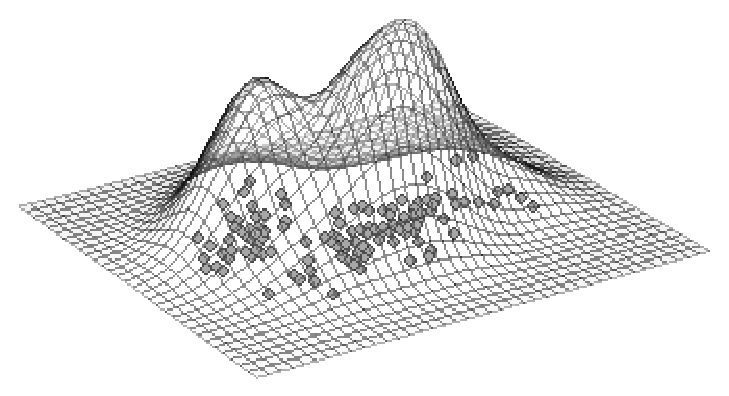
\includegraphics[width=2.5in]{CLUST/density/figs/draftfigs/kde-2d-c}
}{
    \def\scaleF{6.5}
    \def\myh{0.35}
    \scalebox{0.4}{%
    \begin{pspicture}(2,2)(10,7.5)
	\psPoint(5.9, 3.0, 0.000000){p0}
\psdot(p0)
\psPoint(6.9, 3.1, 0.000000){p1}
\psdot(p1)
\psPoint(6.6, 2.9, 0.000000){p2}
\psdot(p2)
\psPoint(4.6, 3.2, 0.000000){p3}
\psdot(p3)
\psPoint(6.0, 2.2, 0.000000){p4}
\psdot(p4)
\psPoint(4.7, 3.2, 0.000000){p5}
\psdot(p5)
\psPoint(6.5, 3.0, 0.000000){p6}
\psdot(p6)
\psPoint(5.8, 2.7, 0.000000){p7}
\psdot(p7)
\psPoint(6.7, 3.1, 0.000000){p8}
\psdot(p8)
\psPoint(6.7, 2.5, 0.000000){p9}
\psdot(p9)
\psPoint(5.1, 3.7, 0.000000){p10}
\psdot(p10)
\psPoint(5.1, 3.8, 0.000000){p11}
\psdot(p11)
\psPoint(5.7, 3.0, 0.000000){p12}
\psdot(p12)
\psPoint(6.1, 3.0, 0.000000){p13}
\psdot(p13)
\psPoint(4.9, 3.1, 0.000000){p14}
\psdot(p14)
\psPoint(5.0, 3.4, 0.000000){p15}
\psdot(p15)
\psPoint(5.0, 3.4, 0.000000){p16}
\psdot(p16)
\psPoint(5.7, 2.8, 0.000000){p17}
\psdot(p17)
\psPoint(5.0, 3.3, 0.000000){p18}
\psdot(p18)
\psPoint(7.2, 3.2, 0.000000){p19}
\psdot(p19)
\psPoint(5.9, 3.0, 0.000000){p20}
\psdot(p20)
\psPoint(6.5, 3.0, 0.000000){p21}
\psdot(p21)
\psPoint(5.7, 4.4, 0.000000){p22}
\psdot(p22)
\psPoint(5.5, 2.5, 0.000000){p23}
\psdot(p23)
\psPoint(4.9, 2.5, 0.000000){p24}
\psdot(p24)
\psPoint(5.0, 3.5, 0.000000){p25}
\psdot(p25)
\psPoint(5.5, 2.3, 0.000000){p26}
\psdot(p26)
\psPoint(4.6, 3.1, 0.000000){p27}
\psdot(p27)
\psPoint(7.2, 3.0, 0.000000){p28}
\psdot(p28)
\psPoint(6.8, 3.2, 0.000000){p29}
\psdot(p29)
\psPoint(5.4, 3.9, 0.000000){p30}
\psdot(p30)
\psPoint(5.0, 3.2, 0.000000){p31}
\psdot(p31)
\psPoint(5.7, 2.5, 0.000000){p32}
\psdot(p32)
\psPoint(5.8, 2.6, 0.000000){p33}
\psdot(p33)
\psPoint(5.1, 2.5, 0.000000){p34}
\psdot(p34)
\psPoint(5.6, 2.5, 0.000000){p35}
\psdot(p35)
\psPoint(5.8, 2.7, 0.000000){p36}
\psdot(p36)
\psPoint(5.1, 3.8, 0.000000){p37}
\psdot(p37)
\psPoint(6.3, 2.3, 0.000000){p38}
\psdot(p38)
\psPoint(6.3, 2.5, 0.000000){p39}
\psdot(p39)
\psPoint(5.6, 3.0, 0.000000){p40}
\psdot(p40)
\psPoint(6.1, 3.0, 0.000000){p41}
\psdot(p41)
\psPoint(6.8, 3.0, 0.000000){p42}
\psdot(p42)
\psPoint(7.3, 2.9, 0.000000){p43}
\psdot(p43)
\psPoint(5.6, 2.7, 0.000000){p44}
\psdot(p44)
\psPoint(4.8, 3.0, 0.000000){p45}
\psdot(p45)
\psPoint(7.1, 3.0, 0.000000){p46}
\psdot(p46)
\psPoint(5.7, 2.6, 0.000000){p47}
\psdot(p47)
\psPoint(5.3, 3.7, 0.000000){p48}
\psdot(p48)
\psPoint(5.7, 3.8, 0.000000){p49}
\psdot(p49)
\psPoint(5.7, 2.9, 0.000000){p50}
\psdot(p50)
\psPoint(5.6, 2.8, 0.000000){p51}
\psdot(p51)
\psPoint(4.4, 3.0, 0.000000){p52}
\psdot(p52)
\psPoint(6.3, 3.3, 0.000000){p53}
\psdot(p53)
\psPoint(5.4, 3.4, 0.000000){p54}
\psdot(p54)
\psPoint(6.3, 3.4, 0.000000){p55}
\psdot(p55)
\psPoint(6.9, 3.1, 0.000000){p56}
\psdot(p56)
\psPoint(7.7, 3.0, 0.000000){p57}
\psdot(p57)
\psPoint(6.1, 2.8, 0.000000){p58}
\psdot(p58)
\psPoint(5.6, 2.9, 0.000000){p59}
\psdot(p59)
\psPoint(6.1, 2.6, 0.000000){p60}
\psdot(p60)
\psPoint(6.4, 2.7, 0.000000){p61}
\psdot(p61)
\psPoint(5.0, 3.5, 0.000000){p62}
\psdot(p62)
\psPoint(5.1, 3.3, 0.000000){p63}
\psdot(p63)
\psPoint(5.6, 3.0, 0.000000){p64}
\psdot(p64)
\psPoint(5.4, 3.0, 0.000000){p65}
\psdot(p65)
\psPoint(5.8, 2.8, 0.000000){p66}
\psdot(p66)
\psPoint(4.9, 3.1, 0.000000){p67}
\psdot(p67)
\psPoint(4.6, 3.6, 0.000000){p68}
\psdot(p68)
\psPoint(5.2, 3.4, 0.000000){p69}
\psdot(p69)
\psPoint(7.9, 3.8, 0.000000){p70}
\psdot(p70)
\psPoint(7.7, 2.6, 0.000000){p71}
\psdot(p71)
\psPoint(6.1, 2.8, 0.000000){p72}
\psdot(p72)
\psPoint(5.5, 3.5, 0.000000){p73}
\psdot(p73)
\psPoint(4.6, 3.4, 0.000000){p74}
\psdot(p74)
\psPoint(4.7, 3.2, 0.000000){p75}
\psdot(p75)
\psPoint(4.4, 2.9, 0.000000){p76}
\psdot(p76)
\psPoint(6.2, 2.8, 0.000000){p77}
\psdot(p77)
\psPoint(4.8, 3.0, 0.000000){p78}
\psdot(p78)
\psPoint(6.0, 2.9, 0.000000){p79}
\psdot(p79)
\psPoint(6.2, 3.4, 0.000000){p80}
\psdot(p80)
\psPoint(5.0, 2.3, 0.000000){p81}
\psdot(p81)
\psPoint(6.4, 3.2, 0.000000){p82}
\psdot(p82)
\psPoint(6.3, 2.9, 0.000000){p83}
\psdot(p83)
\psPoint(6.7, 3.0, 0.000000){p84}
\psdot(p84)
\psPoint(5.0, 2.0, 0.000000){p85}
\psdot(p85)
\psPoint(5.9, 3.2, 0.000000){p86}
\psdot(p86)
\psPoint(6.7, 3.3, 0.000000){p87}
\psdot(p87)
\psPoint(5.4, 3.9, 0.000000){p88}
\psdot(p88)
\psPoint(6.3, 2.7, 0.000000){p89}
\psdot(p89)
\psPoint(4.8, 3.4, 0.000000){p90}
\psdot(p90)
\psPoint(4.4, 3.2, 0.000000){p91}
\psdot(p91)
\psPoint(6.4, 3.2, 0.000000){p92}
\psdot(p92)
\psPoint(6.2, 2.2, 0.000000){p93}
\psdot(p93)
\psPoint(6.0, 2.2, 0.000000){p94}
\psdot(p94)
\psPoint(7.4, 2.8, 0.000000){p95}
\psdot(p95)
\psPoint(4.9, 2.4, 0.000000){p96}
\psdot(p96)
\psPoint(7.0, 3.2, 0.000000){p97}
\psdot(p97)
\psPoint(5.5, 2.4, 0.000000){p98}
\psdot(p98)
\psPoint(6.3, 3.3, 0.000000){p99}
\psdot(p99)
\psPoint(6.8, 2.8, 0.000000){p100}
\psdot(p100)
\psPoint(6.1, 2.9, 0.000000){p101}
\psdot(p101)
\psPoint(6.5, 3.2, 0.000000){p102}
\psdot(p102)
\psPoint(6.7, 3.3, 0.000000){p103}
\psdot(p103)
\psPoint(6.7, 3.1, 0.000000){p104}
\psdot(p104)
\psPoint(4.8, 3.4, 0.000000){p105}
\psdot(p105)
\psPoint(4.9, 3.0, 0.000000){p106}
\psdot(p106)
\psPoint(6.9, 3.2, 0.000000){p107}
\psdot(p107)
\psPoint(4.5, 2.3, 0.000000){p108}
\psdot(p108)
\psPoint(4.3, 3.0, 0.000000){p109}
\psdot(p109)
\psPoint(5.2, 2.7, 0.000000){p110}
\psdot(p110)
\psPoint(5.0, 3.6, 0.000000){p111}
\psdot(p111)
\psPoint(6.4, 2.9, 0.000000){p112}
\psdot(p112)
\psPoint(5.2, 3.5, 0.000000){p113}
\psdot(p113)
\psPoint(5.8, 2.7, 0.000000){p114}
\psdot(p114)
\psPoint(5.5, 4.2, 0.000000){p115}
\psdot(p115)
\psPoint(7.6, 3.0, 0.000000){p116}
\psdot(p116)
\psPoint(6.3, 2.8, 0.000000){p117}
\psdot(p117)
\psPoint(6.4, 3.1, 0.000000){p118}
\psdot(p118)
\psPoint(6.3, 2.5, 0.000000){p119}
\psdot(p119)
\psPoint(5.8, 2.7, 0.000000){p120}
\psdot(p120)
\psPoint(5.0, 3.0, 0.000000){p121}
\psdot(p121)
\psPoint(6.7, 3.1, 0.000000){p122}
\psdot(p122)
\psPoint(6.0, 2.7, 0.000000){p123}
\psdot(p123)
\psPoint(5.1, 3.5, 0.000000){p124}
\psdot(p124)
\psPoint(4.8, 3.1, 0.000000){p125}
\psdot(p125)
\psPoint(5.7, 2.8, 0.000000){p126}
\psdot(p126)
\psPoint(5.1, 3.8, 0.000000){p127}
\psdot(p127)
\psPoint(6.6, 3.0, 0.000000){p128}
\psdot(p128)
\psPoint(6.4, 2.8, 0.000000){p129}
\psdot(p129)
\psPoint(5.2, 4.1, 0.000000){p130}
\psdot(p130)
\psPoint(6.4, 2.8, 0.000000){p131}
\psdot(p131)
\psPoint(7.7, 2.8, 0.000000){p132}
\psdot(p132)
\psPoint(5.8, 4.0, 0.000000){p133}
\psdot(p133)
\psPoint(4.9, 3.1, 0.000000){p134}
\psdot(p134)
\psPoint(5.4, 3.7, 0.000000){p135}
\psdot(p135)
\psPoint(5.1, 3.5, 0.000000){p136}
\psdot(p136)
\psPoint(6.0, 3.4, 0.000000){p137}
\psdot(p137)
\psPoint(6.5, 3.0, 0.000000){p138}
\psdot(p138)
\psPoint(5.5, 2.4, 0.000000){p139}
\psdot(p139)
\psPoint(7.2, 3.6, 0.000000){p140}
\psdot(p140)
\psPoint(6.9, 3.1, 0.000000){p141}
\psdot(p141)
\psPoint(6.2, 2.9, 0.000000){p142}
\psdot(p142)
\psPoint(6.5, 2.8, 0.000000){p143}
\psdot(p143)
\psPoint(6.0, 3.0, 0.000000){p144}
\psdot(p144)
\psPoint(5.4, 3.4, 0.000000){p145}
\psdot(p145)
\psPoint(5.5, 2.6, 0.000000){p146}
\psdot(p146)
\psPoint(6.7, 3.0, 0.000000){p147}
\psdot(p147)
\psPoint(7.7, 3.8, 0.000000){p148}
\psdot(p148)
\psPoint(5.1, 3.4, 0.000000){p149}
\psdot(p149)

	\psset{fillcolor=white}
	\psSurface[ngrid=40 30,	algebraic](3.5,1)(8.5,5){%
\scaleF*(0.001061/\myh^2)*
(e^((-0.5/\myh^2)*((x-5.90)^2 + (y-3.00)^2))+
e^((-0.5/\myh^2)*((x-6.90)^2 + (y-3.10)^2))+
e^((-0.5/\myh^2)*((x-6.60)^2 + (y-2.90)^2))+
e^((-0.5/\myh^2)*((x-4.60)^2 + (y-3.20)^2))+
e^((-0.5/\myh^2)*((x-6.00)^2 + (y-2.20)^2))+
e^((-0.5/\myh^2)*((x-4.70)^2 + (y-3.20)^2))+
e^((-0.5/\myh^2)*((x-6.50)^2 + (y-3.00)^2))+
e^((-0.5/\myh^2)*((x-5.80)^2 + (y-2.70)^2))+
e^((-0.5/\myh^2)*((x-6.70)^2 + (y-3.10)^2))+
e^((-0.5/\myh^2)*((x-6.70)^2 + (y-2.50)^2))+
e^((-0.5/\myh^2)*((x-5.10)^2 + (y-3.70)^2))+
e^((-0.5/\myh^2)*((x-5.10)^2 + (y-3.80)^2))+
e^((-0.5/\myh^2)*((x-5.70)^2 + (y-3.00)^2))+
e^((-0.5/\myh^2)*((x-6.10)^2 + (y-3.00)^2))+
e^((-0.5/\myh^2)*((x-4.90)^2 + (y-3.10)^2))+
e^((-0.5/\myh^2)*((x-5.00)^2 + (y-3.40)^2))+
e^((-0.5/\myh^2)*((x-5.00)^2 + (y-3.40)^2))+
e^((-0.5/\myh^2)*((x-5.70)^2 + (y-2.80)^2))+
e^((-0.5/\myh^2)*((x-5.00)^2 + (y-3.30)^2))+
e^((-0.5/\myh^2)*((x-7.20)^2 + (y-3.20)^2))+
e^((-0.5/\myh^2)*((x-5.90)^2 + (y-3.00)^2))+
e^((-0.5/\myh^2)*((x-6.50)^2 + (y-3.00)^2))+
e^((-0.5/\myh^2)*((x-5.70)^2 + (y-4.40)^2))+
e^((-0.5/\myh^2)*((x-5.50)^2 + (y-2.50)^2))+
e^((-0.5/\myh^2)*((x-4.90)^2 + (y-2.50)^2))+
e^((-0.5/\myh^2)*((x-5.00)^2 + (y-3.50)^2))+
e^((-0.5/\myh^2)*((x-5.50)^2 + (y-2.30)^2))+
e^((-0.5/\myh^2)*((x-4.60)^2 + (y-3.10)^2))+
e^((-0.5/\myh^2)*((x-7.20)^2 + (y-3.00)^2))+
e^((-0.5/\myh^2)*((x-6.80)^2 + (y-3.20)^2))+
e^((-0.5/\myh^2)*((x-5.40)^2 + (y-3.90)^2))+
e^((-0.5/\myh^2)*((x-5.00)^2 + (y-3.20)^2))+
e^((-0.5/\myh^2)*((x-5.70)^2 + (y-2.50)^2))+
e^((-0.5/\myh^2)*((x-5.80)^2 + (y-2.60)^2))+
e^((-0.5/\myh^2)*((x-5.10)^2 + (y-2.50)^2))+
e^((-0.5/\myh^2)*((x-5.60)^2 + (y-2.50)^2))+
e^((-0.5/\myh^2)*((x-5.80)^2 + (y-2.70)^2))+
e^((-0.5/\myh^2)*((x-5.10)^2 + (y-3.80)^2))+
e^((-0.5/\myh^2)*((x-6.30)^2 + (y-2.30)^2))+
e^((-0.5/\myh^2)*((x-6.30)^2 + (y-2.50)^2))+
e^((-0.5/\myh^2)*((x-5.60)^2 + (y-3.00)^2))+
e^((-0.5/\myh^2)*((x-6.10)^2 + (y-3.00)^2))+
e^((-0.5/\myh^2)*((x-6.80)^2 + (y-3.00)^2))+
e^((-0.5/\myh^2)*((x-7.30)^2 + (y-2.90)^2))+
e^((-0.5/\myh^2)*((x-5.60)^2 + (y-2.70)^2))+
e^((-0.5/\myh^2)*((x-4.80)^2 + (y-3.00)^2))+
e^((-0.5/\myh^2)*((x-7.10)^2 + (y-3.00)^2))+
e^((-0.5/\myh^2)*((x-5.70)^2 + (y-2.60)^2))+
e^((-0.5/\myh^2)*((x-5.30)^2 + (y-3.70)^2))+
e^((-0.5/\myh^2)*((x-5.70)^2 + (y-3.80)^2))+
e^((-0.5/\myh^2)*((x-5.70)^2 + (y-2.90)^2))+
e^((-0.5/\myh^2)*((x-5.60)^2 + (y-2.80)^2))+
e^((-0.5/\myh^2)*((x-4.40)^2 + (y-3.00)^2))+
e^((-0.5/\myh^2)*((x-6.30)^2 + (y-3.30)^2))+
e^((-0.5/\myh^2)*((x-5.40)^2 + (y-3.40)^2))+
e^((-0.5/\myh^2)*((x-6.30)^2 + (y-3.40)^2))+
e^((-0.5/\myh^2)*((x-6.90)^2 + (y-3.10)^2))+
e^((-0.5/\myh^2)*((x-7.70)^2 + (y-3.00)^2))+
e^((-0.5/\myh^2)*((x-6.10)^2 + (y-2.80)^2))+
e^((-0.5/\myh^2)*((x-5.60)^2 + (y-2.90)^2))+
e^((-0.5/\myh^2)*((x-6.10)^2 + (y-2.60)^2))+
e^((-0.5/\myh^2)*((x-6.40)^2 + (y-2.70)^2))+
e^((-0.5/\myh^2)*((x-5.00)^2 + (y-3.50)^2))+
e^((-0.5/\myh^2)*((x-5.10)^2 + (y-3.30)^2))+
e^((-0.5/\myh^2)*((x-5.60)^2 + (y-3.00)^2))+
e^((-0.5/\myh^2)*((x-5.40)^2 + (y-3.00)^2))+
e^((-0.5/\myh^2)*((x-5.80)^2 + (y-2.80)^2))+
e^((-0.5/\myh^2)*((x-4.90)^2 + (y-3.10)^2))+
e^((-0.5/\myh^2)*((x-4.60)^2 + (y-3.60)^2))+
e^((-0.5/\myh^2)*((x-5.20)^2 + (y-3.40)^2))+
e^((-0.5/\myh^2)*((x-7.90)^2 + (y-3.80)^2))+
e^((-0.5/\myh^2)*((x-7.70)^2 + (y-2.60)^2))+
e^((-0.5/\myh^2)*((x-6.10)^2 + (y-2.80)^2))+
e^((-0.5/\myh^2)*((x-5.50)^2 + (y-3.50)^2))+
e^((-0.5/\myh^2)*((x-4.60)^2 + (y-3.40)^2))+
e^((-0.5/\myh^2)*((x-4.70)^2 + (y-3.20)^2))+
e^((-0.5/\myh^2)*((x-4.40)^2 + (y-2.90)^2))+
e^((-0.5/\myh^2)*((x-6.20)^2 + (y-2.80)^2))+
e^((-0.5/\myh^2)*((x-4.80)^2 + (y-3.00)^2))+
e^((-0.5/\myh^2)*((x-6.00)^2 + (y-2.90)^2))+
e^((-0.5/\myh^2)*((x-6.20)^2 + (y-3.40)^2))+
e^((-0.5/\myh^2)*((x-5.00)^2 + (y-2.30)^2))+
e^((-0.5/\myh^2)*((x-6.40)^2 + (y-3.20)^2))+
e^((-0.5/\myh^2)*((x-6.30)^2 + (y-2.90)^2))+
e^((-0.5/\myh^2)*((x-6.70)^2 + (y-3.00)^2))+
e^((-0.5/\myh^2)*((x-5.00)^2 + (y-2.00)^2))+
e^((-0.5/\myh^2)*((x-5.90)^2 + (y-3.20)^2))+
e^((-0.5/\myh^2)*((x-6.70)^2 + (y-3.30)^2))+
e^((-0.5/\myh^2)*((x-5.40)^2 + (y-3.90)^2))+
e^((-0.5/\myh^2)*((x-6.30)^2 + (y-2.70)^2))+
e^((-0.5/\myh^2)*((x-4.80)^2 + (y-3.40)^2))+
e^((-0.5/\myh^2)*((x-4.40)^2 + (y-3.20)^2))+
e^((-0.5/\myh^2)*((x-6.40)^2 + (y-3.20)^2))+
e^((-0.5/\myh^2)*((x-6.20)^2 + (y-2.20)^2))+
e^((-0.5/\myh^2)*((x-6.00)^2 + (y-2.20)^2))+
e^((-0.5/\myh^2)*((x-7.40)^2 + (y-2.80)^2))+
e^((-0.5/\myh^2)*((x-4.90)^2 + (y-2.40)^2))+
e^((-0.5/\myh^2)*((x-7.00)^2 + (y-3.20)^2))+
e^((-0.5/\myh^2)*((x-5.50)^2 + (y-2.40)^2))+
e^((-0.5/\myh^2)*((x-6.30)^2 + (y-3.30)^2))+
e^((-0.5/\myh^2)*((x-6.80)^2 + (y-2.80)^2))+
e^((-0.5/\myh^2)*((x-6.10)^2 + (y-2.90)^2))+
e^((-0.5/\myh^2)*((x-6.50)^2 + (y-3.20)^2))+
e^((-0.5/\myh^2)*((x-6.70)^2 + (y-3.30)^2))+
e^((-0.5/\myh^2)*((x-6.70)^2 + (y-3.10)^2))+
e^((-0.5/\myh^2)*((x-4.80)^2 + (y-3.40)^2))+
e^((-0.5/\myh^2)*((x-4.90)^2 + (y-3.00)^2))+
e^((-0.5/\myh^2)*((x-6.90)^2 + (y-3.20)^2))+
e^((-0.5/\myh^2)*((x-4.50)^2 + (y-2.30)^2))+
e^((-0.5/\myh^2)*((x-4.30)^2 + (y-3.00)^2))+
e^((-0.5/\myh^2)*((x-5.20)^2 + (y-2.70)^2))+
e^((-0.5/\myh^2)*((x-5.00)^2 + (y-3.60)^2))+
e^((-0.5/\myh^2)*((x-6.40)^2 + (y-2.90)^2))+
e^((-0.5/\myh^2)*((x-5.20)^2 + (y-3.50)^2))+
e^((-0.5/\myh^2)*((x-5.80)^2 + (y-2.70)^2))+
e^((-0.5/\myh^2)*((x-5.50)^2 + (y-4.20)^2))+
e^((-0.5/\myh^2)*((x-7.60)^2 + (y-3.00)^2))+
e^((-0.5/\myh^2)*((x-6.30)^2 + (y-2.80)^2))+
e^((-0.5/\myh^2)*((x-6.40)^2 + (y-3.10)^2))+
e^((-0.5/\myh^2)*((x-6.30)^2 + (y-2.50)^2))+
e^((-0.5/\myh^2)*((x-5.80)^2 + (y-2.70)^2))+
e^((-0.5/\myh^2)*((x-5.00)^2 + (y-3.00)^2))+
e^((-0.5/\myh^2)*((x-6.70)^2 + (y-3.10)^2))+
e^((-0.5/\myh^2)*((x-6.00)^2 + (y-2.70)^2))+
e^((-0.5/\myh^2)*((x-5.10)^2 + (y-3.50)^2))+
e^((-0.5/\myh^2)*((x-4.80)^2 + (y-3.10)^2))+
e^((-0.5/\myh^2)*((x-5.70)^2 + (y-2.80)^2))+
e^((-0.5/\myh^2)*((x-5.10)^2 + (y-3.80)^2))+
e^((-0.5/\myh^2)*((x-6.60)^2 + (y-3.00)^2))+
e^((-0.5/\myh^2)*((x-6.40)^2 + (y-2.80)^2))+
e^((-0.5/\myh^2)*((x-5.20)^2 + (y-4.10)^2))+
e^((-0.5/\myh^2)*((x-6.40)^2 + (y-2.80)^2))+
e^((-0.5/\myh^2)*((x-7.70)^2 + (y-2.80)^2))+
e^((-0.5/\myh^2)*((x-5.80)^2 + (y-4.00)^2))+
e^((-0.5/\myh^2)*((x-4.90)^2 + (y-3.10)^2))+
e^((-0.5/\myh^2)*((x-5.40)^2 + (y-3.70)^2))+
e^((-0.5/\myh^2)*((x-5.10)^2 + (y-3.50)^2))+
e^((-0.5/\myh^2)*((x-6.00)^2 + (y-3.40)^2))+
e^((-0.5/\myh^2)*((x-6.50)^2 + (y-3.00)^2))+
e^((-0.5/\myh^2)*((x-5.50)^2 + (y-2.40)^2))+
e^((-0.5/\myh^2)*((x-7.20)^2 + (y-3.60)^2))+
e^((-0.5/\myh^2)*((x-6.90)^2 + (y-3.10)^2))+
e^((-0.5/\myh^2)*((x-6.20)^2 + (y-2.90)^2))+
e^((-0.5/\myh^2)*((x-6.50)^2 + (y-2.80)^2))+
e^((-0.5/\myh^2)*((x-6.00)^2 + (y-3.00)^2))+
e^((-0.5/\myh^2)*((x-5.40)^2 + (y-3.40)^2))+
e^((-0.5/\myh^2)*((x-5.50)^2 + (y-2.60)^2))+
e^((-0.5/\myh^2)*((x-6.70)^2 + (y-3.00)^2))+
e^((-0.5/\myh^2)*((x-7.70)^2 + (y-3.80)^2))+
e^((-0.5/\myh^2)*((x-5.10)^2 + (y-3.40)^2)))
}
\end{pspicture}


    }
    }}
    \vspace{0.1in}
\subfloat[$h=0.6$]{
\label{fig:clust:den:kde2dGd}
\ifdraft{
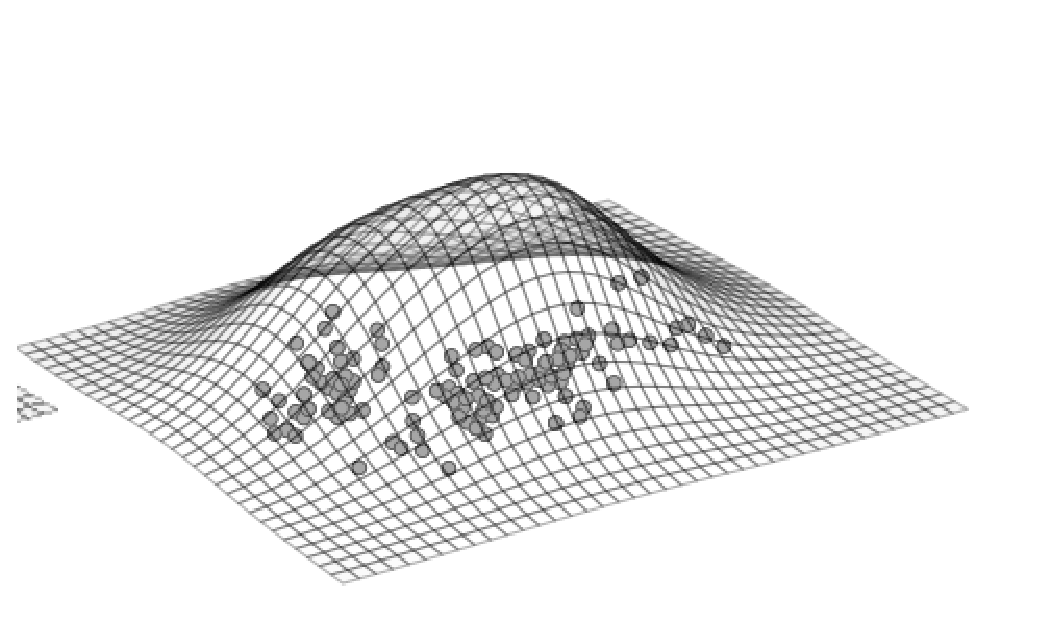
\includegraphics[width=2.5in]{CLUST/density/figs/draftfigs/kde-2d-d}
}{
    \def\scaleF{7.5}
    \def\myh{0.6}
    \scalebox{0.4}{%
    \begin{pspicture}(2,2)(10,7.5)
	\psPoint(5.9, 3.0, 0.000000){p0}
\psdot(p0)
\psPoint(6.9, 3.1, 0.000000){p1}
\psdot(p1)
\psPoint(6.6, 2.9, 0.000000){p2}
\psdot(p2)
\psPoint(4.6, 3.2, 0.000000){p3}
\psdot(p3)
\psPoint(6.0, 2.2, 0.000000){p4}
\psdot(p4)
\psPoint(4.7, 3.2, 0.000000){p5}
\psdot(p5)
\psPoint(6.5, 3.0, 0.000000){p6}
\psdot(p6)
\psPoint(5.8, 2.7, 0.000000){p7}
\psdot(p7)
\psPoint(6.7, 3.1, 0.000000){p8}
\psdot(p8)
\psPoint(6.7, 2.5, 0.000000){p9}
\psdot(p9)
\psPoint(5.1, 3.7, 0.000000){p10}
\psdot(p10)
\psPoint(5.1, 3.8, 0.000000){p11}
\psdot(p11)
\psPoint(5.7, 3.0, 0.000000){p12}
\psdot(p12)
\psPoint(6.1, 3.0, 0.000000){p13}
\psdot(p13)
\psPoint(4.9, 3.1, 0.000000){p14}
\psdot(p14)
\psPoint(5.0, 3.4, 0.000000){p15}
\psdot(p15)
\psPoint(5.0, 3.4, 0.000000){p16}
\psdot(p16)
\psPoint(5.7, 2.8, 0.000000){p17}
\psdot(p17)
\psPoint(5.0, 3.3, 0.000000){p18}
\psdot(p18)
\psPoint(7.2, 3.2, 0.000000){p19}
\psdot(p19)
\psPoint(5.9, 3.0, 0.000000){p20}
\psdot(p20)
\psPoint(6.5, 3.0, 0.000000){p21}
\psdot(p21)
\psPoint(5.7, 4.4, 0.000000){p22}
\psdot(p22)
\psPoint(5.5, 2.5, 0.000000){p23}
\psdot(p23)
\psPoint(4.9, 2.5, 0.000000){p24}
\psdot(p24)
\psPoint(5.0, 3.5, 0.000000){p25}
\psdot(p25)
\psPoint(5.5, 2.3, 0.000000){p26}
\psdot(p26)
\psPoint(4.6, 3.1, 0.000000){p27}
\psdot(p27)
\psPoint(7.2, 3.0, 0.000000){p28}
\psdot(p28)
\psPoint(6.8, 3.2, 0.000000){p29}
\psdot(p29)
\psPoint(5.4, 3.9, 0.000000){p30}
\psdot(p30)
\psPoint(5.0, 3.2, 0.000000){p31}
\psdot(p31)
\psPoint(5.7, 2.5, 0.000000){p32}
\psdot(p32)
\psPoint(5.8, 2.6, 0.000000){p33}
\psdot(p33)
\psPoint(5.1, 2.5, 0.000000){p34}
\psdot(p34)
\psPoint(5.6, 2.5, 0.000000){p35}
\psdot(p35)
\psPoint(5.8, 2.7, 0.000000){p36}
\psdot(p36)
\psPoint(5.1, 3.8, 0.000000){p37}
\psdot(p37)
\psPoint(6.3, 2.3, 0.000000){p38}
\psdot(p38)
\psPoint(6.3, 2.5, 0.000000){p39}
\psdot(p39)
\psPoint(5.6, 3.0, 0.000000){p40}
\psdot(p40)
\psPoint(6.1, 3.0, 0.000000){p41}
\psdot(p41)
\psPoint(6.8, 3.0, 0.000000){p42}
\psdot(p42)
\psPoint(7.3, 2.9, 0.000000){p43}
\psdot(p43)
\psPoint(5.6, 2.7, 0.000000){p44}
\psdot(p44)
\psPoint(4.8, 3.0, 0.000000){p45}
\psdot(p45)
\psPoint(7.1, 3.0, 0.000000){p46}
\psdot(p46)
\psPoint(5.7, 2.6, 0.000000){p47}
\psdot(p47)
\psPoint(5.3, 3.7, 0.000000){p48}
\psdot(p48)
\psPoint(5.7, 3.8, 0.000000){p49}
\psdot(p49)
\psPoint(5.7, 2.9, 0.000000){p50}
\psdot(p50)
\psPoint(5.6, 2.8, 0.000000){p51}
\psdot(p51)
\psPoint(4.4, 3.0, 0.000000){p52}
\psdot(p52)
\psPoint(6.3, 3.3, 0.000000){p53}
\psdot(p53)
\psPoint(5.4, 3.4, 0.000000){p54}
\psdot(p54)
\psPoint(6.3, 3.4, 0.000000){p55}
\psdot(p55)
\psPoint(6.9, 3.1, 0.000000){p56}
\psdot(p56)
\psPoint(7.7, 3.0, 0.000000){p57}
\psdot(p57)
\psPoint(6.1, 2.8, 0.000000){p58}
\psdot(p58)
\psPoint(5.6, 2.9, 0.000000){p59}
\psdot(p59)
\psPoint(6.1, 2.6, 0.000000){p60}
\psdot(p60)
\psPoint(6.4, 2.7, 0.000000){p61}
\psdot(p61)
\psPoint(5.0, 3.5, 0.000000){p62}
\psdot(p62)
\psPoint(5.1, 3.3, 0.000000){p63}
\psdot(p63)
\psPoint(5.6, 3.0, 0.000000){p64}
\psdot(p64)
\psPoint(5.4, 3.0, 0.000000){p65}
\psdot(p65)
\psPoint(5.8, 2.8, 0.000000){p66}
\psdot(p66)
\psPoint(4.9, 3.1, 0.000000){p67}
\psdot(p67)
\psPoint(4.6, 3.6, 0.000000){p68}
\psdot(p68)
\psPoint(5.2, 3.4, 0.000000){p69}
\psdot(p69)
\psPoint(7.9, 3.8, 0.000000){p70}
\psdot(p70)
\psPoint(7.7, 2.6, 0.000000){p71}
\psdot(p71)
\psPoint(6.1, 2.8, 0.000000){p72}
\psdot(p72)
\psPoint(5.5, 3.5, 0.000000){p73}
\psdot(p73)
\psPoint(4.6, 3.4, 0.000000){p74}
\psdot(p74)
\psPoint(4.7, 3.2, 0.000000){p75}
\psdot(p75)
\psPoint(4.4, 2.9, 0.000000){p76}
\psdot(p76)
\psPoint(6.2, 2.8, 0.000000){p77}
\psdot(p77)
\psPoint(4.8, 3.0, 0.000000){p78}
\psdot(p78)
\psPoint(6.0, 2.9, 0.000000){p79}
\psdot(p79)
\psPoint(6.2, 3.4, 0.000000){p80}
\psdot(p80)
\psPoint(5.0, 2.3, 0.000000){p81}
\psdot(p81)
\psPoint(6.4, 3.2, 0.000000){p82}
\psdot(p82)
\psPoint(6.3, 2.9, 0.000000){p83}
\psdot(p83)
\psPoint(6.7, 3.0, 0.000000){p84}
\psdot(p84)
\psPoint(5.0, 2.0, 0.000000){p85}
\psdot(p85)
\psPoint(5.9, 3.2, 0.000000){p86}
\psdot(p86)
\psPoint(6.7, 3.3, 0.000000){p87}
\psdot(p87)
\psPoint(5.4, 3.9, 0.000000){p88}
\psdot(p88)
\psPoint(6.3, 2.7, 0.000000){p89}
\psdot(p89)
\psPoint(4.8, 3.4, 0.000000){p90}
\psdot(p90)
\psPoint(4.4, 3.2, 0.000000){p91}
\psdot(p91)
\psPoint(6.4, 3.2, 0.000000){p92}
\psdot(p92)
\psPoint(6.2, 2.2, 0.000000){p93}
\psdot(p93)
\psPoint(6.0, 2.2, 0.000000){p94}
\psdot(p94)
\psPoint(7.4, 2.8, 0.000000){p95}
\psdot(p95)
\psPoint(4.9, 2.4, 0.000000){p96}
\psdot(p96)
\psPoint(7.0, 3.2, 0.000000){p97}
\psdot(p97)
\psPoint(5.5, 2.4, 0.000000){p98}
\psdot(p98)
\psPoint(6.3, 3.3, 0.000000){p99}
\psdot(p99)
\psPoint(6.8, 2.8, 0.000000){p100}
\psdot(p100)
\psPoint(6.1, 2.9, 0.000000){p101}
\psdot(p101)
\psPoint(6.5, 3.2, 0.000000){p102}
\psdot(p102)
\psPoint(6.7, 3.3, 0.000000){p103}
\psdot(p103)
\psPoint(6.7, 3.1, 0.000000){p104}
\psdot(p104)
\psPoint(4.8, 3.4, 0.000000){p105}
\psdot(p105)
\psPoint(4.9, 3.0, 0.000000){p106}
\psdot(p106)
\psPoint(6.9, 3.2, 0.000000){p107}
\psdot(p107)
\psPoint(4.5, 2.3, 0.000000){p108}
\psdot(p108)
\psPoint(4.3, 3.0, 0.000000){p109}
\psdot(p109)
\psPoint(5.2, 2.7, 0.000000){p110}
\psdot(p110)
\psPoint(5.0, 3.6, 0.000000){p111}
\psdot(p111)
\psPoint(6.4, 2.9, 0.000000){p112}
\psdot(p112)
\psPoint(5.2, 3.5, 0.000000){p113}
\psdot(p113)
\psPoint(5.8, 2.7, 0.000000){p114}
\psdot(p114)
\psPoint(5.5, 4.2, 0.000000){p115}
\psdot(p115)
\psPoint(7.6, 3.0, 0.000000){p116}
\psdot(p116)
\psPoint(6.3, 2.8, 0.000000){p117}
\psdot(p117)
\psPoint(6.4, 3.1, 0.000000){p118}
\psdot(p118)
\psPoint(6.3, 2.5, 0.000000){p119}
\psdot(p119)
\psPoint(5.8, 2.7, 0.000000){p120}
\psdot(p120)
\psPoint(5.0, 3.0, 0.000000){p121}
\psdot(p121)
\psPoint(6.7, 3.1, 0.000000){p122}
\psdot(p122)
\psPoint(6.0, 2.7, 0.000000){p123}
\psdot(p123)
\psPoint(5.1, 3.5, 0.000000){p124}
\psdot(p124)
\psPoint(4.8, 3.1, 0.000000){p125}
\psdot(p125)
\psPoint(5.7, 2.8, 0.000000){p126}
\psdot(p126)
\psPoint(5.1, 3.8, 0.000000){p127}
\psdot(p127)
\psPoint(6.6, 3.0, 0.000000){p128}
\psdot(p128)
\psPoint(6.4, 2.8, 0.000000){p129}
\psdot(p129)
\psPoint(5.2, 4.1, 0.000000){p130}
\psdot(p130)
\psPoint(6.4, 2.8, 0.000000){p131}
\psdot(p131)
\psPoint(7.7, 2.8, 0.000000){p132}
\psdot(p132)
\psPoint(5.8, 4.0, 0.000000){p133}
\psdot(p133)
\psPoint(4.9, 3.1, 0.000000){p134}
\psdot(p134)
\psPoint(5.4, 3.7, 0.000000){p135}
\psdot(p135)
\psPoint(5.1, 3.5, 0.000000){p136}
\psdot(p136)
\psPoint(6.0, 3.4, 0.000000){p137}
\psdot(p137)
\psPoint(6.5, 3.0, 0.000000){p138}
\psdot(p138)
\psPoint(5.5, 2.4, 0.000000){p139}
\psdot(p139)
\psPoint(7.2, 3.6, 0.000000){p140}
\psdot(p140)
\psPoint(6.9, 3.1, 0.000000){p141}
\psdot(p141)
\psPoint(6.2, 2.9, 0.000000){p142}
\psdot(p142)
\psPoint(6.5, 2.8, 0.000000){p143}
\psdot(p143)
\psPoint(6.0, 3.0, 0.000000){p144}
\psdot(p144)
\psPoint(5.4, 3.4, 0.000000){p145}
\psdot(p145)
\psPoint(5.5, 2.6, 0.000000){p146}
\psdot(p146)
\psPoint(6.7, 3.0, 0.000000){p147}
\psdot(p147)
\psPoint(7.7, 3.8, 0.000000){p148}
\psdot(p148)
\psPoint(5.1, 3.4, 0.000000){p149}
\psdot(p149)

	\psset{fillcolor=white}
	\psSurface[ngrid=40 30,	algebraic](3.5,1)(8.5,5){%
\scaleF*(0.001061/\myh^2)*
(e^((-0.5/\myh^2)*((x-5.90)^2 + (y-3.00)^2))+
e^((-0.5/\myh^2)*((x-6.90)^2 + (y-3.10)^2))+
e^((-0.5/\myh^2)*((x-6.60)^2 + (y-2.90)^2))+
e^((-0.5/\myh^2)*((x-4.60)^2 + (y-3.20)^2))+
e^((-0.5/\myh^2)*((x-6.00)^2 + (y-2.20)^2))+
e^((-0.5/\myh^2)*((x-4.70)^2 + (y-3.20)^2))+
e^((-0.5/\myh^2)*((x-6.50)^2 + (y-3.00)^2))+
e^((-0.5/\myh^2)*((x-5.80)^2 + (y-2.70)^2))+
e^((-0.5/\myh^2)*((x-6.70)^2 + (y-3.10)^2))+
e^((-0.5/\myh^2)*((x-6.70)^2 + (y-2.50)^2))+
e^((-0.5/\myh^2)*((x-5.10)^2 + (y-3.70)^2))+
e^((-0.5/\myh^2)*((x-5.10)^2 + (y-3.80)^2))+
e^((-0.5/\myh^2)*((x-5.70)^2 + (y-3.00)^2))+
e^((-0.5/\myh^2)*((x-6.10)^2 + (y-3.00)^2))+
e^((-0.5/\myh^2)*((x-4.90)^2 + (y-3.10)^2))+
e^((-0.5/\myh^2)*((x-5.00)^2 + (y-3.40)^2))+
e^((-0.5/\myh^2)*((x-5.00)^2 + (y-3.40)^2))+
e^((-0.5/\myh^2)*((x-5.70)^2 + (y-2.80)^2))+
e^((-0.5/\myh^2)*((x-5.00)^2 + (y-3.30)^2))+
e^((-0.5/\myh^2)*((x-7.20)^2 + (y-3.20)^2))+
e^((-0.5/\myh^2)*((x-5.90)^2 + (y-3.00)^2))+
e^((-0.5/\myh^2)*((x-6.50)^2 + (y-3.00)^2))+
e^((-0.5/\myh^2)*((x-5.70)^2 + (y-4.40)^2))+
e^((-0.5/\myh^2)*((x-5.50)^2 + (y-2.50)^2))+
e^((-0.5/\myh^2)*((x-4.90)^2 + (y-2.50)^2))+
e^((-0.5/\myh^2)*((x-5.00)^2 + (y-3.50)^2))+
e^((-0.5/\myh^2)*((x-5.50)^2 + (y-2.30)^2))+
e^((-0.5/\myh^2)*((x-4.60)^2 + (y-3.10)^2))+
e^((-0.5/\myh^2)*((x-7.20)^2 + (y-3.00)^2))+
e^((-0.5/\myh^2)*((x-6.80)^2 + (y-3.20)^2))+
e^((-0.5/\myh^2)*((x-5.40)^2 + (y-3.90)^2))+
e^((-0.5/\myh^2)*((x-5.00)^2 + (y-3.20)^2))+
e^((-0.5/\myh^2)*((x-5.70)^2 + (y-2.50)^2))+
e^((-0.5/\myh^2)*((x-5.80)^2 + (y-2.60)^2))+
e^((-0.5/\myh^2)*((x-5.10)^2 + (y-2.50)^2))+
e^((-0.5/\myh^2)*((x-5.60)^2 + (y-2.50)^2))+
e^((-0.5/\myh^2)*((x-5.80)^2 + (y-2.70)^2))+
e^((-0.5/\myh^2)*((x-5.10)^2 + (y-3.80)^2))+
e^((-0.5/\myh^2)*((x-6.30)^2 + (y-2.30)^2))+
e^((-0.5/\myh^2)*((x-6.30)^2 + (y-2.50)^2))+
e^((-0.5/\myh^2)*((x-5.60)^2 + (y-3.00)^2))+
e^((-0.5/\myh^2)*((x-6.10)^2 + (y-3.00)^2))+
e^((-0.5/\myh^2)*((x-6.80)^2 + (y-3.00)^2))+
e^((-0.5/\myh^2)*((x-7.30)^2 + (y-2.90)^2))+
e^((-0.5/\myh^2)*((x-5.60)^2 + (y-2.70)^2))+
e^((-0.5/\myh^2)*((x-4.80)^2 + (y-3.00)^2))+
e^((-0.5/\myh^2)*((x-7.10)^2 + (y-3.00)^2))+
e^((-0.5/\myh^2)*((x-5.70)^2 + (y-2.60)^2))+
e^((-0.5/\myh^2)*((x-5.30)^2 + (y-3.70)^2))+
e^((-0.5/\myh^2)*((x-5.70)^2 + (y-3.80)^2))+
e^((-0.5/\myh^2)*((x-5.70)^2 + (y-2.90)^2))+
e^((-0.5/\myh^2)*((x-5.60)^2 + (y-2.80)^2))+
e^((-0.5/\myh^2)*((x-4.40)^2 + (y-3.00)^2))+
e^((-0.5/\myh^2)*((x-6.30)^2 + (y-3.30)^2))+
e^((-0.5/\myh^2)*((x-5.40)^2 + (y-3.40)^2))+
e^((-0.5/\myh^2)*((x-6.30)^2 + (y-3.40)^2))+
e^((-0.5/\myh^2)*((x-6.90)^2 + (y-3.10)^2))+
e^((-0.5/\myh^2)*((x-7.70)^2 + (y-3.00)^2))+
e^((-0.5/\myh^2)*((x-6.10)^2 + (y-2.80)^2))+
e^((-0.5/\myh^2)*((x-5.60)^2 + (y-2.90)^2))+
e^((-0.5/\myh^2)*((x-6.10)^2 + (y-2.60)^2))+
e^((-0.5/\myh^2)*((x-6.40)^2 + (y-2.70)^2))+
e^((-0.5/\myh^2)*((x-5.00)^2 + (y-3.50)^2))+
e^((-0.5/\myh^2)*((x-5.10)^2 + (y-3.30)^2))+
e^((-0.5/\myh^2)*((x-5.60)^2 + (y-3.00)^2))+
e^((-0.5/\myh^2)*((x-5.40)^2 + (y-3.00)^2))+
e^((-0.5/\myh^2)*((x-5.80)^2 + (y-2.80)^2))+
e^((-0.5/\myh^2)*((x-4.90)^2 + (y-3.10)^2))+
e^((-0.5/\myh^2)*((x-4.60)^2 + (y-3.60)^2))+
e^((-0.5/\myh^2)*((x-5.20)^2 + (y-3.40)^2))+
e^((-0.5/\myh^2)*((x-7.90)^2 + (y-3.80)^2))+
e^((-0.5/\myh^2)*((x-7.70)^2 + (y-2.60)^2))+
e^((-0.5/\myh^2)*((x-6.10)^2 + (y-2.80)^2))+
e^((-0.5/\myh^2)*((x-5.50)^2 + (y-3.50)^2))+
e^((-0.5/\myh^2)*((x-4.60)^2 + (y-3.40)^2))+
e^((-0.5/\myh^2)*((x-4.70)^2 + (y-3.20)^2))+
e^((-0.5/\myh^2)*((x-4.40)^2 + (y-2.90)^2))+
e^((-0.5/\myh^2)*((x-6.20)^2 + (y-2.80)^2))+
e^((-0.5/\myh^2)*((x-4.80)^2 + (y-3.00)^2))+
e^((-0.5/\myh^2)*((x-6.00)^2 + (y-2.90)^2))+
e^((-0.5/\myh^2)*((x-6.20)^2 + (y-3.40)^2))+
e^((-0.5/\myh^2)*((x-5.00)^2 + (y-2.30)^2))+
e^((-0.5/\myh^2)*((x-6.40)^2 + (y-3.20)^2))+
e^((-0.5/\myh^2)*((x-6.30)^2 + (y-2.90)^2))+
e^((-0.5/\myh^2)*((x-6.70)^2 + (y-3.00)^2))+
e^((-0.5/\myh^2)*((x-5.00)^2 + (y-2.00)^2))+
e^((-0.5/\myh^2)*((x-5.90)^2 + (y-3.20)^2))+
e^((-0.5/\myh^2)*((x-6.70)^2 + (y-3.30)^2))+
e^((-0.5/\myh^2)*((x-5.40)^2 + (y-3.90)^2))+
e^((-0.5/\myh^2)*((x-6.30)^2 + (y-2.70)^2))+
e^((-0.5/\myh^2)*((x-4.80)^2 + (y-3.40)^2))+
e^((-0.5/\myh^2)*((x-4.40)^2 + (y-3.20)^2))+
e^((-0.5/\myh^2)*((x-6.40)^2 + (y-3.20)^2))+
e^((-0.5/\myh^2)*((x-6.20)^2 + (y-2.20)^2))+
e^((-0.5/\myh^2)*((x-6.00)^2 + (y-2.20)^2))+
e^((-0.5/\myh^2)*((x-7.40)^2 + (y-2.80)^2))+
e^((-0.5/\myh^2)*((x-4.90)^2 + (y-2.40)^2))+
e^((-0.5/\myh^2)*((x-7.00)^2 + (y-3.20)^2))+
e^((-0.5/\myh^2)*((x-5.50)^2 + (y-2.40)^2))+
e^((-0.5/\myh^2)*((x-6.30)^2 + (y-3.30)^2))+
e^((-0.5/\myh^2)*((x-6.80)^2 + (y-2.80)^2))+
e^((-0.5/\myh^2)*((x-6.10)^2 + (y-2.90)^2))+
e^((-0.5/\myh^2)*((x-6.50)^2 + (y-3.20)^2))+
e^((-0.5/\myh^2)*((x-6.70)^2 + (y-3.30)^2))+
e^((-0.5/\myh^2)*((x-6.70)^2 + (y-3.10)^2))+
e^((-0.5/\myh^2)*((x-4.80)^2 + (y-3.40)^2))+
e^((-0.5/\myh^2)*((x-4.90)^2 + (y-3.00)^2))+
e^((-0.5/\myh^2)*((x-6.90)^2 + (y-3.20)^2))+
e^((-0.5/\myh^2)*((x-4.50)^2 + (y-2.30)^2))+
e^((-0.5/\myh^2)*((x-4.30)^2 + (y-3.00)^2))+
e^((-0.5/\myh^2)*((x-5.20)^2 + (y-2.70)^2))+
e^((-0.5/\myh^2)*((x-5.00)^2 + (y-3.60)^2))+
e^((-0.5/\myh^2)*((x-6.40)^2 + (y-2.90)^2))+
e^((-0.5/\myh^2)*((x-5.20)^2 + (y-3.50)^2))+
e^((-0.5/\myh^2)*((x-5.80)^2 + (y-2.70)^2))+
e^((-0.5/\myh^2)*((x-5.50)^2 + (y-4.20)^2))+
e^((-0.5/\myh^2)*((x-7.60)^2 + (y-3.00)^2))+
e^((-0.5/\myh^2)*((x-6.30)^2 + (y-2.80)^2))+
e^((-0.5/\myh^2)*((x-6.40)^2 + (y-3.10)^2))+
e^((-0.5/\myh^2)*((x-6.30)^2 + (y-2.50)^2))+
e^((-0.5/\myh^2)*((x-5.80)^2 + (y-2.70)^2))+
e^((-0.5/\myh^2)*((x-5.00)^2 + (y-3.00)^2))+
e^((-0.5/\myh^2)*((x-6.70)^2 + (y-3.10)^2))+
e^((-0.5/\myh^2)*((x-6.00)^2 + (y-2.70)^2))+
e^((-0.5/\myh^2)*((x-5.10)^2 + (y-3.50)^2))+
e^((-0.5/\myh^2)*((x-4.80)^2 + (y-3.10)^2))+
e^((-0.5/\myh^2)*((x-5.70)^2 + (y-2.80)^2))+
e^((-0.5/\myh^2)*((x-5.10)^2 + (y-3.80)^2))+
e^((-0.5/\myh^2)*((x-6.60)^2 + (y-3.00)^2))+
e^((-0.5/\myh^2)*((x-6.40)^2 + (y-2.80)^2))+
e^((-0.5/\myh^2)*((x-5.20)^2 + (y-4.10)^2))+
e^((-0.5/\myh^2)*((x-6.40)^2 + (y-2.80)^2))+
e^((-0.5/\myh^2)*((x-7.70)^2 + (y-2.80)^2))+
e^((-0.5/\myh^2)*((x-5.80)^2 + (y-4.00)^2))+
e^((-0.5/\myh^2)*((x-4.90)^2 + (y-3.10)^2))+
e^((-0.5/\myh^2)*((x-5.40)^2 + (y-3.70)^2))+
e^((-0.5/\myh^2)*((x-5.10)^2 + (y-3.50)^2))+
e^((-0.5/\myh^2)*((x-6.00)^2 + (y-3.40)^2))+
e^((-0.5/\myh^2)*((x-6.50)^2 + (y-3.00)^2))+
e^((-0.5/\myh^2)*((x-5.50)^2 + (y-2.40)^2))+
e^((-0.5/\myh^2)*((x-7.20)^2 + (y-3.60)^2))+
e^((-0.5/\myh^2)*((x-6.90)^2 + (y-3.10)^2))+
e^((-0.5/\myh^2)*((x-6.20)^2 + (y-2.90)^2))+
e^((-0.5/\myh^2)*((x-6.50)^2 + (y-2.80)^2))+
e^((-0.5/\myh^2)*((x-6.00)^2 + (y-3.00)^2))+
e^((-0.5/\myh^2)*((x-5.40)^2 + (y-3.40)^2))+
e^((-0.5/\myh^2)*((x-5.50)^2 + (y-2.60)^2))+
e^((-0.5/\myh^2)*((x-6.70)^2 + (y-3.00)^2))+
e^((-0.5/\myh^2)*((x-7.70)^2 + (y-3.80)^2))+
e^((-0.5/\myh^2)*((x-5.10)^2 + (y-3.40)^2)))
}
\end{pspicture}


    }
    }}
    }
\end{figure}
\end{frame}



\begin{frame}{Density Estimation: Density-based Dataset}
  \framesubtitle{Gaussian kernel, $h=20$}
\begin{figure}
%%  \label{fig:clust:den:kdeShape}
%%\end{figure}
%\begin{figure}[t!]%fig15.8
%  \centering
%  \ifdraft{%
    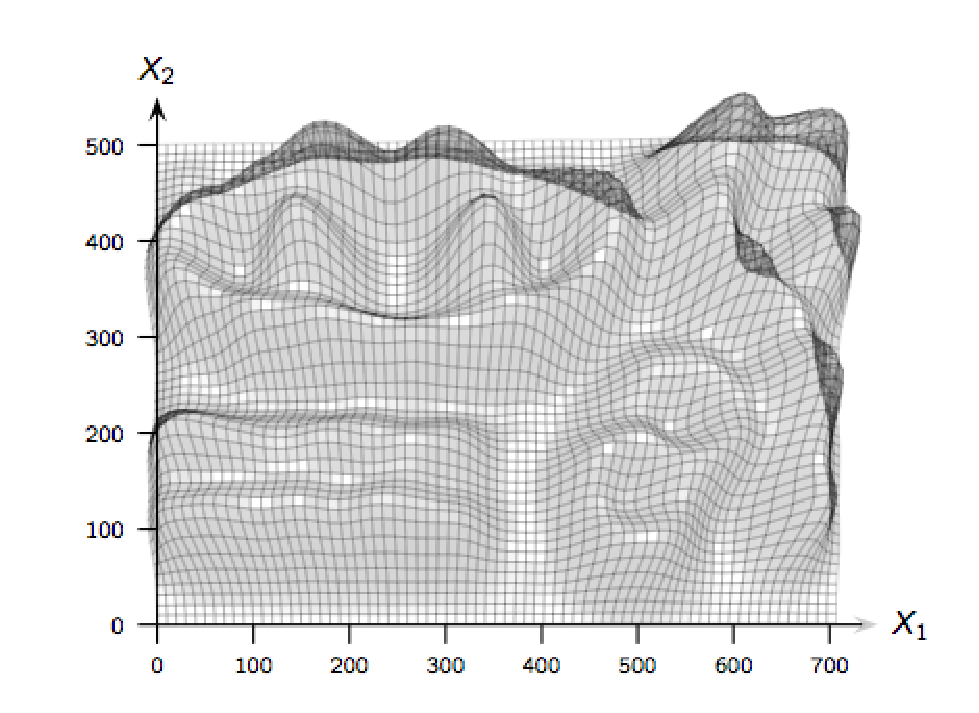
\includegraphics[scale=0.6]{CLUST/density/figs/draftfigs/kdeShape.eps}
%  }{
%%\comment{%
%\psset{unit=0.5in}
%\psset{viewpoint=70 90 91 rtp2xyz,Decran=65}
%\psset{lightsrc=viewpoint}
%\defFunction[algebraic]{myfunc}(u,v){u}{v}{((v^2)-(u^2))/4}
%\begin{pspicture}(-1,-0.5)(7,6)
%%\psSolid[object=surfaceparametree, action=writeobj,
%%  file=CLUST/density/figs/mysurf,
%%  ngrid=1.0 1.0,incolor=white, fillcolor=lightgray,
%%  linewidth=0.5\pslinewidth,function=myfunc,base=0.0 7.0 0.0 5.0]
%\psPoint(0,0,0){O2}
%\psPoint(7.75,0,0){X2}
%\psPoint(0,5.5,0){Y2}
%\psline[arrows=->,arrowscale=2](O2)(X2)
%\psline[arrows=->,arrowscale=2](O2)(Y2)
%\uput[r](X2){$X_1$}
%\uput[u](Y2){$X_2$}
%%\psset{dotstyle=Bo,fillcolor=gray,linecolor=lightgray}
%%\psset{dotsize=0.05}
%%\psPoint(5.73663, 4.62705, 3.000000){p0}
\psdot(p0)
\psPoint(2.72958, 3.58739, 3.000000){p1}
\psdot(p1)
\psPoint(4.88711, 2.18802, 3.000000){p2}
\psdot(p2)
\psPoint(0.2647, 3.53756, 3.000000){p3}
\psdot(p3)
\psPoint(3.91275, 4.10433, 3.000000){p4}
\psdot(p4)
\psPoint(6.36726, 2.28562, 3.000000){p5}
\psdot(p5)
\psPoint(1.37104, 2.71697, 3.000000){p6}
\psdot(p6)
\psPoint(5.26954, 4.2366, 3.000000){p7}
\psdot(p7)
\psPoint(4.40992, 0.62826, 3.000000){p8}
\psdot(p8)
\psPoint(3.30697, 3.51166, 3.000000){p9}
\psdot(p9)
\psPoint(3.14221, 4.11265, 3.000000){p10}
\psdot(p10)
\psPoint(1.82901, 3.51725, 3.000000){p11}
\psdot(p11)
\psPoint(6.28531, 1.50092, 3.000000){p12}
\psdot(p12)
\psPoint(6.6524, 4.09595, 3.000000){p13}
\psdot(p13)
\psPoint(1.60336, 2.75217, 3.000000){p14}
\psdot(p14)
\psPoint(5.09416, 1.3411, 3.000000){p15}
\psdot(p15)
\psPoint(2.68271, 1.44971, 3.000000){p16}
\psdot(p16)
\psPoint(4.324, 3.88274, 3.000000){p17}
\psdot(p17)
\psPoint(3.10828, 4.04414, 3.000000){p18}
\psdot(p18)
\psPoint(6.22866, 3.28758, 3.000000){p19}
\psdot(p19)
\psPoint(5.60466, 3.53041, 3.000000){p20}
\psdot(p20)
\psPoint(5.35098, 4.57578, 3.000000){p21}
\psdot(p21)
\psPoint(1.62748, 3.6749, 3.000000){p22}
\psdot(p22)
\psPoint(2.28702, 1.04394, 3.000000){p23}
\psdot(p23)
\psPoint(5.33845, 1.23349, 3.000000){p24}
\psdot(p24)
\psPoint(6.25158, 2.4282, 3.000000){p25}
\psdot(p25)
\psPoint(1.94606, 2.60517, 3.000000){p26}
\psdot(p26)
\psPoint(3.13138, 3.04009, 3.000000){p27}
\psdot(p27)
\psPoint(1.34019, 2.82918, 3.000000){p28}
\psdot(p28)
\psPoint(5.63753, 2.31232, 3.000000){p29}
\psdot(p29)
\psPoint(6.10765, 2.15919, 3.000000){p30}
\psdot(p30)
\psPoint(4.20488, 2.78139, 3.000000){p31}
\psdot(p31)
\psPoint(2.7114, 3.45803, 3.000000){p32}
\psdot(p32)
\psPoint(6.38583, 3.6565, 3.000000){p33}
\psdot(p33)
\psPoint(3.27559, 1.11013, 3.000000){p34}
\psdot(p34)
\psPoint(1.47269, 1.83251, 3.000000){p35}
\psdot(p35)
\psPoint(6.29318, 4.52661, 3.000000){p36}
\psdot(p36)
\psPoint(2.00888, 1.6863, 3.000000){p37}
\psdot(p37)
\psPoint(2.76389, 1.63719, 3.000000){p38}
\psdot(p38)
\psPoint(2.2185, 4.40864, 3.000000){p39}
\psdot(p39)
\psPoint(1.06713, 1.58568, 3.000000){p40}
\psdot(p40)
\psPoint(3.14936, 3.24915, 3.000000){p41}
\psdot(p41)
\psPoint(3.77075, 4.2577, 3.000000){p42}
\psdot(p42)
\psPoint(6.74818, 3.24548, 3.000000){p43}
\psdot(p43)
\psPoint(4.98069, 2.45935, 3.000000){p44}
\psdot(p44)
\psPoint(5.08035, 2.15328, 3.000000){p45}
\psdot(p45)
\psPoint(1.2955, 3.45552, 3.000000){p46}
\psdot(p46)
\psPoint(3.19688, 3.6028, 3.000000){p47}
\psdot(p47)
\psPoint(1.6331, 3.52216, 3.000000){p48}
\psdot(p48)
\psPoint(0.79592, 0.76397, 3.000000){p49}
\psdot(p49)
\psPoint(4.01346, 2.78385, 3.000000){p50}
\psdot(p50)
\psPoint(2.72275, 4.45758, 3.000000){p51}
\psdot(p51)
\psPoint(3.45812, 2.72642, 3.000000){p52}
\psdot(p52)
\psPoint(4.65386, 2.11468, 3.000000){p53}
\psdot(p53)
\psPoint(1.50459, 2.37566, 3.000000){p54}
\psdot(p54)
\psPoint(0.55135, 3.82346, 3.000000){p55}
\psdot(p55)
\psPoint(2.71278, 3.3212, 3.000000){p56}
\psdot(p56)
\psPoint(3.65264, 2.61569, 3.000000){p57}
\psdot(p57)
\psPoint(5.52828, 3.04859, 3.000000){p58}
\psdot(p58)
\psPoint(6.09945, 1.58653, 3.000000){p59}
\psdot(p59)
\psPoint(1.42781, 3.16362, 3.000000){p60}
\psdot(p60)
\psPoint(2.53523, 4.32818, 3.000000){p61}
\psdot(p61)
\psPoint(2.21221, 3.44022, 3.000000){p62}
\psdot(p62)
\psPoint(1.95446, 2.59275, 3.000000){p63}
\psdot(p63)
\psPoint(6.6288, 1.14582, 3.000000){p64}
\psdot(p64)
\psPoint(3.22503, 1.37376, 3.000000){p65}
\psdot(p65)
\psPoint(2.63353, 4.04726, 3.000000){p66}
\psdot(p66)
\psPoint(1.7918, 2.79618, 3.000000){p67}
\psdot(p67)
\psPoint(2.26701, 2.43069, 3.000000){p68}
\psdot(p68)
\psPoint(2.01895, 4.21718, 3.000000){p69}
\psdot(p69)
\psPoint(2.49635, 1.47358, 3.000000){p70}
\psdot(p70)
\psPoint(0.33276, 1.12226, 3.000000){p71}
\psdot(p71)
\psPoint(4.90376, 0.60239, 3.000000){p72}
\psdot(p72)
\psPoint(6.43405, 2.36404, 3.000000){p73}
\psdot(p73)
\psPoint(1.79363, 3.43574, 3.000000){p74}
\psdot(p74)
\psPoint(2.37357, 1.79362, 3.000000){p75}
\psdot(p75)
\psPoint(5.7449, 1.53965, 3.000000){p76}
\psdot(p76)
\psPoint(4.21076, 3.21448, 3.000000){p77}
\psdot(p77)
\psPoint(3.64513, 3.30463, 3.000000){p78}
\psdot(p78)
\psPoint(2.4378, 0.99689, 3.000000){p79}
\psdot(p79)
\psPoint(4.07023, 4.15673, 3.000000){p80}
\psdot(p80)
\psPoint(1.4818, 0.7151, 3.000000){p81}
\psdot(p81)
\psPoint(6.60578, 1.18683, 3.000000){p82}
\psdot(p82)
\psPoint(2.1271, 1.80665, 3.000000){p83}
\psdot(p83)
\psPoint(2.83488, 1.00249, 3.000000){p84}
\psdot(p84)
\psPoint(1.69333, 0.98483, 3.000000){p85}
\psdot(p85)
\psPoint(5.96785, 3.95191, 3.000000){p86}
\psdot(p86)
\psPoint(2.92148, 3.02648, 3.000000){p87}
\psdot(p87)
\psPoint(2.43962, 4.40814, 3.000000){p88}
\psdot(p88)
\psPoint(0.26873, 1.70355, 3.000000){p89}
\psdot(p89)
\psPoint(0.22939, 0.88756, 3.000000){p90}
\psdot(p90)
\psPoint(3.42257, 3.05089, 3.000000){p91}
\psdot(p91)
\psPoint(0.7893, 2.78739, 3.000000){p92}
\psdot(p92)
\psPoint(6.41912, 0.69422, 3.000000){p93}
\psdot(p93)
\psPoint(3.35147, 3.14891, 3.000000){p94}
\psdot(p94)
\psPoint(1.93055, 4.36953, 3.000000){p95}
\psdot(p95)
\psPoint(3.65041, 2.72918, 3.000000){p96}
\psdot(p96)
\psPoint(0.40033, 0.74325, 3.000000){p97}
\psdot(p97)
\psPoint(0.54094, 0.6893, 3.000000){p98}
\psdot(p98)
\psPoint(1.98517, 0.97118, 3.000000){p99}
\psdot(p99)
\psPoint(3.30539, 1.64632, 3.000000){p100}
\psdot(p100)
\psPoint(4.23694, 1.3456, 3.000000){p101}
\psdot(p101)
\psPoint(1.91472, 3.47015, 3.000000){p102}
\psdot(p102)
\psPoint(2.20093, 4.15472, 3.000000){p103}
\psdot(p103)
\psPoint(6.23064, 3.5785, 3.000000){p104}
\psdot(p104)
\psPoint(1.70007, 2.65446, 3.000000){p105}
\psdot(p105)
\psPoint(1.24455, 4.15932, 3.000000){p106}
\psdot(p106)
\psPoint(6.43697, 2.3382, 3.000000){p107}
\psdot(p107)
\psPoint(0.66523, 2.83799, 3.000000){p108}
\psdot(p108)
\psPoint(0.92504, 2.66296, 3.000000){p109}
\psdot(p109)
\psPoint(6.07416, 1.88377, 3.000000){p110}
\psdot(p110)
\psPoint(2.82745, 2.46628, 3.000000){p111}
\psdot(p111)
\psPoint(5.57546, 1.83663, 3.000000){p112}
\psdot(p112)
\psPoint(2.76517, 4.05353, 3.000000){p113}
\psdot(p113)
\psPoint(3.01349, 1.5568, 3.000000){p114}
\psdot(p114)
\psPoint(2.45933, 2.47694, 3.000000){p115}
\psdot(p115)
\psPoint(6.28105, 3.47213, 3.000000){p116}
\psdot(p116)
\psPoint(6.3499, 4.49028, 3.000000){p117}
\psdot(p117)
\psPoint(4.73044, 1.693, 3.000000){p118}
\psdot(p118)
\psPoint(1.91319, 4.09425, 3.000000){p119}
\psdot(p119)
\psPoint(6.30689, 1.45696, 3.000000){p120}
\psdot(p120)
\psPoint(5.45515, 2.05062, 3.000000){p121}
\psdot(p121)
\psPoint(0.87172, 2.84134, 3.000000){p122}
\psdot(p122)
\psPoint(5.26582, 0.75995, 3.000000){p123}
\psdot(p123)
\psPoint(3.45197, 3.5103, 3.000000){p124}
\psdot(p124)
\psPoint(5.49355, 4.10475, 3.000000){p125}
\psdot(p125)
\psPoint(4.12013, 2.73039, 3.000000){p126}
\psdot(p126)
\psPoint(0.75356, 1.0483, 3.000000){p127}
\psdot(p127)
\psPoint(1.62154, 1.12124, 3.000000){p128}
\psdot(p128)
\psPoint(2.23541, 2.58017, 3.000000){p129}
\psdot(p129)
\psPoint(5.55218, 1.55698, 3.000000){p130}
\psdot(p130)
\psPoint(0.68767, 2.1258, 3.000000){p131}
\psdot(p131)
\psPoint(5.05604, 0.80587, 3.000000){p132}
\psdot(p132)
\psPoint(2.55987, 4.15031, 3.000000){p133}
\psdot(p133)
\psPoint(3.54939, 1.31378, 3.000000){p134}
\psdot(p134)
\psPoint(4.93986, 4.52359, 3.000000){p135}
\psdot(p135)
\psPoint(2.95339, 1.61434, 3.000000){p136}
\psdot(p136)
\psPoint(4.23311, 2.01298, 3.000000){p137}
\psdot(p137)
\psPoint(3.19884, 3.13587, 3.000000){p138}
\psdot(p138)
\psPoint(4.74385, 1.66211, 3.000000){p139}
\psdot(p139)
\psPoint(6.39365, 1.63731, 3.000000){p140}
\psdot(p140)
\psPoint(5.16499, 1.19602, 3.000000){p141}
\psdot(p141)
\psPoint(5.48895, 3.53427, 3.000000){p142}
\psdot(p142)
\psPoint(6.31181, 0.90578, 3.000000){p143}
\psdot(p143)
\psPoint(5.31025, 4.09594, 3.000000){p144}
\psdot(p144)
\psPoint(1.92684, 4.13771, 3.000000){p145}
\psdot(p145)
\psPoint(1.26147, 4.26478, 3.000000){p146}
\psdot(p146)
\psPoint(0.63907, 3.71659, 3.000000){p147}
\psdot(p147)
\psPoint(4.33522, 3.8791, 3.000000){p148}
\psdot(p148)
\psPoint(0.2488, 1.78809, 3.000000){p149}
\psdot(p149)
\psPoint(2.80907, 0.75983, 3.000000){p150}
\psdot(p150)
\psPoint(2.34124, 2.693, 3.000000){p151}
\psdot(p151)
\psPoint(1.18043, 2.68763, 3.000000){p152}
\psdot(p152)
\psPoint(1.33566, 3.24192, 3.000000){p153}
\psdot(p153)
\psPoint(1.24917, 4.16612, 3.000000){p154}
\psdot(p154)
\psPoint(1.35319, 1.82999, 3.000000){p155}
\psdot(p155)
\psPoint(1.85582, 1.59981, 3.000000){p156}
\psdot(p156)
\psPoint(4.72289, 1.70258, 3.000000){p157}
\psdot(p157)
\psPoint(4.38462, 3.28804, 3.000000){p158}
\psdot(p158)
\psPoint(3.1386, 3.74769, 3.000000){p159}
\psdot(p159)
\psPoint(1.57031, 1.38417, 3.000000){p160}
\psdot(p160)
\psPoint(3.57676, 3.14311, 3.000000){p161}
\psdot(p161)
\psPoint(1.56265, 0.40148, 3.000000){p162}
\psdot(p162)
\psPoint(1.3951, 3.6332, 3.000000){p163}
\psdot(p163)
\psPoint(1.13792, 3.89306, 3.000000){p164}
\psdot(p164)
\psPoint(0.65201, 4.00415, 3.000000){p165}
\psdot(p165)
\psPoint(0.44926, 3.0539, 3.000000){p166}
\psdot(p166)
\psPoint(5.58751, 4.16916, 3.000000){p167}
\psdot(p167)
\psPoint(6.05976, 2.1104, 3.000000){p168}
\psdot(p168)
\psPoint(6.02285, 3.7345, 3.000000){p169}
\psdot(p169)
\psPoint(1.32272, 3.1766, 3.000000){p170}
\psdot(p170)
\psPoint(1.71561, 2.8003, 3.000000){p171}
\psdot(p171)
\psPoint(6.01888, 4.37302, 3.000000){p172}
\psdot(p172)
\psPoint(4.51057, 1.47524, 3.000000){p173}
\psdot(p173)
\psPoint(4.63561, 0.83951, 3.000000){p174}
\psdot(p174)
\psPoint(1.57916, 1.92259, 3.000000){p175}
\psdot(p175)
\psPoint(0.82632, 0.90993, 3.000000){p176}
\psdot(p176)
\psPoint(0.40363, 1.72293, 3.000000){p177}
\psdot(p177)
\psPoint(6.06236, 2.20902, 3.000000){p178}
\psdot(p178)
\psPoint(3.68392, 4.11804, 3.000000){p179}
\psdot(p179)
\psPoint(5.33909, 4.47317, 3.000000){p180}
\psdot(p180)
\psPoint(5.82308, 4.31827, 3.000000){p181}
\psdot(p181)
\psPoint(1.84201, 2.71984, 3.000000){p182}
\psdot(p182)
\psPoint(6.26318, 3.2178, 3.000000){p183}
\psdot(p183)
\psPoint(0.65152, 0.87445, 3.000000){p184}
\psdot(p184)
\psPoint(5.67278, 4.00157, 3.000000){p185}
\psdot(p185)
\psPoint(1.6136, 1.58388, 3.000000){p186}
\psdot(p186)
\psPoint(3.16973, 4.29696, 3.000000){p187}
\psdot(p187)
\psPoint(2.09105, 4.33396, 3.000000){p188}
\psdot(p188)
\psPoint(4.72407, 3.62644, 3.000000){p189}
\psdot(p189)
\psPoint(6.23942, 2.42762, 3.000000){p190}
\psdot(p190)
\psPoint(5.88914, 3.13694, 3.000000){p191}
\psdot(p191)
\psPoint(6.44574, 1.09599, 3.000000){p192}
\psdot(p192)
\psPoint(6.83215, 3.28168, 3.000000){p193}
\psdot(p193)
\psPoint(6.01327, 4.17243, 3.000000){p194}
\psdot(p194)
\psPoint(5.0772, 3.54306, 3.000000){p195}
\psdot(p195)
\psPoint(2.54236, 0.84097, 3.000000){p196}
\psdot(p196)
\psPoint(6.25616, 1.96519, 3.000000){p197}
\psdot(p197)
\psPoint(0.43105, 3.5388, 3.000000){p198}
\psdot(p198)
\psPoint(6.52831, 2.0227, 3.000000){p199}
\psdot(p199)
\psPoint(4.93472, 1.72017, 3.000000){p200}
\psdot(p200)
\psPoint(0.75768, 3.86666, 3.000000){p201}
\psdot(p201)
\psPoint(6.71685, 3.6448, 3.000000){p202}
\psdot(p202)
\psPoint(6.26168, 3.25358, 3.000000){p203}
\psdot(p203)
\psPoint(2.16678, 0.52878, 3.000000){p204}
\psdot(p204)
\psPoint(5.16723, 1.39649, 3.000000){p205}
\psdot(p205)
\psPoint(0.31262, 2.27115, 3.000000){p206}
\psdot(p206)
\psPoint(5.22584, 1.07244, 3.000000){p207}
\psdot(p207)
\psPoint(2.01416, 1.63788, 3.000000){p208}
\psdot(p208)
\psPoint(3.77341, 2.59234, 3.000000){p209}
\psdot(p209)
\psPoint(4.74275, 2.27441, 3.000000){p210}
\psdot(p210)
\psPoint(1.59964, 1.3839, 3.000000){p211}
\psdot(p211)
\psPoint(0.69485, 1.10585, 3.000000){p212}
\psdot(p212)
\psPoint(4.5654, 3.02206, 3.000000){p213}
\psdot(p213)
\psPoint(3.45122, 2.81928, 3.000000){p214}
\psdot(p214)
\psPoint(5.09961, 0.88616, 3.000000){p215}
\psdot(p215)
\psPoint(3.37224, 4.34136, 3.000000){p216}
\psdot(p216)
\psPoint(4.12508, 3.97621, 3.000000){p217}
\psdot(p217)
\psPoint(0.7401, 0.73671, 3.000000){p218}
\psdot(p218)
\psPoint(5.36621, 4.48563, 3.000000){p219}
\psdot(p219)
\psPoint(1.43467, 4.25734, 3.000000){p220}
\psdot(p220)
\psPoint(4.26936, 3.83646, 3.000000){p221}
\psdot(p221)
\psPoint(0.98283, 1.02789, 3.000000){p222}
\psdot(p222)
\psPoint(5.50675, 3.27448, 3.000000){p223}
\psdot(p223)
\psPoint(1.87395, 1.52099, 3.000000){p224}
\psdot(p224)
\psPoint(3.38582, 3.97027, 3.000000){p225}
\psdot(p225)
\psPoint(1.99447, 0.91465, 3.000000){p226}
\psdot(p226)
\psPoint(0.55245, 0.77925, 3.000000){p227}
\psdot(p227)
\psPoint(5.64601, 3.66443, 3.000000){p228}
\psdot(p228)
\psPoint(5.30758, 3.38816, 3.000000){p229}
\psdot(p229)
\psPoint(6.6143, 3.72276, 3.000000){p230}
\psdot(p230)
\psPoint(6.33869, 1.88259, 3.000000){p231}
\psdot(p231)
\psPoint(0.80111, 1.56644, 3.000000){p232}
\psdot(p232)
\psPoint(3.74516, 3.01581, 3.000000){p233}
\psdot(p233)
\psPoint(5.67845, 4.14547, 3.000000){p234}
\psdot(p234)
\psPoint(5.54264, 2.99127, 3.000000){p235}
\psdot(p235)
\psPoint(1.68283, 2.5795, 3.000000){p236}
\psdot(p236)
\psPoint(1.58359, 1.11598, 3.000000){p237}
\psdot(p237)
\psPoint(1.28238, 4.29041, 3.000000){p238}
\psdot(p238)
\psPoint(4.56452, 0.70104, 3.000000){p239}
\psdot(p239)
\psPoint(1.9673, 2.63448, 3.000000){p240}
\psdot(p240)
\psPoint(1.0041, 0.97905, 3.000000){p241}
\psdot(p241)
\psPoint(5.75176, 1.53382, 3.000000){p242}
\psdot(p242)
\psPoint(5.52192, 4.23151, 3.000000){p243}
\psdot(p243)
\psPoint(2.17973, 1.70295, 3.000000){p244}
\psdot(p244)
\psPoint(0.25923, 0.70788, 3.000000){p245}
\psdot(p245)
\psPoint(6.05508, 2.25926, 3.000000){p246}
\psdot(p246)
\psPoint(4.41551, 3.4523, 3.000000){p247}
\psdot(p247)
\psPoint(5.47195, 4.24432, 3.000000){p248}
\psdot(p248)
\psPoint(1.67199, 2.5512, 3.000000){p249}
\psdot(p249)
\psPoint(2.30877, 4.36569, 3.000000){p250}
\psdot(p250)
\psPoint(0.58391, 3.14439, 3.000000){p251}
\psdot(p251)
\psPoint(3.24897, 2.62238, 3.000000){p252}
\psdot(p252)
\psPoint(6.2659, 2.25893, 3.000000){p253}
\psdot(p253)
\psPoint(6.6, 4.47613, 3.000000){p254}
\psdot(p254)
\psPoint(0.43668, 2.91399, 3.000000){p255}
\psdot(p255)
\psPoint(6.73834, 4.35254, 3.000000){p256}
\psdot(p256)
\psPoint(1.04347, 1.75611, 3.000000){p257}
\psdot(p257)
\psPoint(3.17203, 1.06982, 3.000000){p258}
\psdot(p258)
\psPoint(0.63116, 3.69837, 3.000000){p259}
\psdot(p259)
\psPoint(1.56759, 4.00334, 3.000000){p260}
\psdot(p260)
\psPoint(6.30543, 2.66906, 3.000000){p261}
\psdot(p261)
\psPoint(0.50432, 2.99391, 3.000000){p262}
\psdot(p262)
\psPoint(5.17639, 4.20626, 3.000000){p263}
\psdot(p263)
\psPoint(6.50768, 3.47282, 3.000000){p264}
\psdot(p264)
\psPoint(1.65121, 3.45513, 3.000000){p265}
\psdot(p265)
\psPoint(5.34698, 3.63307, 3.000000){p266}
\psdot(p266)
\psPoint(6.40128, 1.95589, 3.000000){p267}
\psdot(p267)
\psPoint(6.07945, 2.87715, 3.000000){p268}
\psdot(p268)
\psPoint(2.49584, 1.40167, 3.000000){p269}
\psdot(p269)
\psPoint(4.90302, 0.50079, 3.000000){p270}
\psdot(p270)
\psPoint(5.15194, 2.2245, 3.000000){p271}
\psdot(p271)
\psPoint(2.06045, 4.36023, 3.000000){p272}
\psdot(p272)
\psPoint(6.32503, 3.33636, 3.000000){p273}
\psdot(p273)
\psPoint(3.58222, 3.39086, 3.000000){p274}
\psdot(p274)
\psPoint(3.51077, 3.15341, 3.000000){p275}
\psdot(p275)
\psPoint(2.69046, 4.15209, 3.000000){p276}
\psdot(p276)
\psPoint(5.35199, 3.80906, 3.000000){p277}
\psdot(p277)
\psPoint(6.36148, 4.22864, 3.000000){p278}
\psdot(p278)
\psPoint(0.36111, 2.99347, 3.000000){p279}
\psdot(p279)
\psPoint(0.71835, 4.68426, 3.000000){p280}
\psdot(p280)
\psPoint(2.7267, 0.49079, 3.000000){p281}
\psdot(p281)
\psPoint(1.7103, 4.03242, 3.000000){p282}
\psdot(p282)
\psPoint(0.97422, 2.24053, 3.000000){p283}
\psdot(p283)
\psPoint(0.21128, 3.11598, 3.000000){p284}
\psdot(p284)
\psPoint(1.68941, 1.65506, 3.000000){p285}
\psdot(p285)
\psPoint(6.45005, 1.67336, 3.000000){p286}
\psdot(p286)
\psPoint(2.81878, 4.07031, 3.000000){p287}
\psdot(p287)
\psPoint(6.39466, 3.12162, 3.000000){p288}
\psdot(p288)
\psPoint(6.47406, 1.65395, 3.000000){p289}
\psdot(p289)
\psPoint(3.79223, 2.72997, 3.000000){p290}
\psdot(p290)
\psPoint(6.59622, 3.03381, 3.000000){p291}
\psdot(p291)
\psPoint(4.63956, 3.5492, 3.000000){p292}
\psdot(p292)
\psPoint(4.72749, 1.4843, 3.000000){p293}
\psdot(p293)
\psPoint(2.72765, 3.40341, 3.000000){p294}
\psdot(p294)
\psPoint(5.77438, 2.69242, 3.000000){p295}
\psdot(p295)
\psPoint(0.69475, 1.7223, 3.000000){p296}
\psdot(p296)
\psPoint(6.09168, 2.4507, 3.000000){p297}
\psdot(p297)
\psPoint(3.37386, 4.21004, 3.000000){p298}
\psdot(p298)
\psPoint(2.20006, 4.32739, 3.000000){p299}
\psdot(p299)
\psPoint(4.48146, 3.93502, 3.000000){p300}
\psdot(p300)
\psPoint(3.30506, 1.32799, 3.000000){p301}
\psdot(p301)
\psPoint(2.37464, 4.26733, 3.000000){p302}
\psdot(p302)
\psPoint(5.36556, 4.17417, 3.000000){p303}
\psdot(p303)
\psPoint(3.20408, 0.71723, 3.000000){p304}
\psdot(p304)
\psPoint(2.8883, 1.41494, 3.000000){p305}
\psdot(p305)
\psPoint(0.55153, 3.81593, 3.000000){p306}
\psdot(p306)
\psPoint(4.93319, 1.3526, 3.000000){p307}
\psdot(p307)
\psPoint(2.07055, 4.27265, 3.000000){p308}
\psdot(p308)
\psPoint(5.49898, 1.82936, 3.000000){p309}
\psdot(p309)
\psPoint(6.7724, 1.71324, 3.000000){p310}
\psdot(p310)
\psPoint(5.27402, 3.94848, 3.000000){p311}
\psdot(p311)
\psPoint(4.82287, 0.72297, 3.000000){p312}
\psdot(p312)
\psPoint(5.12532, 2.48172, 3.000000){p313}
\psdot(p313)
\psPoint(6.55928, 3.31411, 3.000000){p314}
\psdot(p314)
\psPoint(6.38076, 3.95519, 3.000000){p315}
\psdot(p315)
\psPoint(6.42192, 1.18147, 3.000000){p316}
\psdot(p316)
\psPoint(2.93233, 2.73559, 3.000000){p317}
\psdot(p317)
\psPoint(1.16626, 2.98558, 3.000000){p318}
\psdot(p318)
\psPoint(5.45988, 4.37964, 3.000000){p319}
\psdot(p319)
\psPoint(0.61127, 0.9923, 3.000000){p320}
\psdot(p320)
\psPoint(0.67919, 1.83032, 3.000000){p321}
\psdot(p321)
\psPoint(4.46962, 3.24436, 3.000000){p322}
\psdot(p322)
\psPoint(0.54469, 3.21346, 3.000000){p323}
\psdot(p323)
\psPoint(4.44529, 3.76501, 3.000000){p324}
\psdot(p324)
\psPoint(5.44441, 4.46594, 3.000000){p325}
\psdot(p325)
\psPoint(3.78167, 2.64315, 3.000000){p326}
\psdot(p326)
\psPoint(4.3546, 3.48163, 3.000000){p327}
\psdot(p327)
\psPoint(6.88904, 4.00265, 3.000000){p328}
\psdot(p328)
\psPoint(5.32918, 1.29125, 3.000000){p329}
\psdot(p329)
\psPoint(5.68816, 4.43492, 3.000000){p330}
\psdot(p330)
\psPoint(5.57338, 2.99815, 3.000000){p331}
\psdot(p331)
\psPoint(6.4714, 1.08757, 3.000000){p332}
\psdot(p332)
\psPoint(3.38683, 3.45399, 3.000000){p333}
\psdot(p333)
\psPoint(1.87419, 0.79655, 3.000000){p334}
\psdot(p334)
\psPoint(0.97908, 2.33809, 3.000000){p335}
\psdot(p335)
\psPoint(3.31139, 2.70079, 3.000000){p336}
\psdot(p336)
\psPoint(5.93909, 2.52438, 3.000000){p337}
\psdot(p337)
\psPoint(4.47242, 1.45226, 3.000000){p338}
\psdot(p338)
\psPoint(0.18958, 3.71422, 3.000000){p339}
\psdot(p339)
\psPoint(3.88146, 3.86002, 3.000000){p340}
\psdot(p340)
\psPoint(1.02495, 0.76782, 3.000000){p341}
\psdot(p341)
\psPoint(6.79437, 3.21916, 3.000000){p342}
\psdot(p342)
\psPoint(1.07186, 1.09662, 3.000000){p343}
\psdot(p343)
\psPoint(6.66254, 3.66738, 3.000000){p344}
\psdot(p344)
\psPoint(6.26247, 1.92001, 3.000000){p345}
\psdot(p345)
\psPoint(5.43797, 1.53217, 3.000000){p346}
\psdot(p346)
\psPoint(6.14086, 2.82568, 3.000000){p347}
\psdot(p347)
\psPoint(0.57621, 2.04114, 3.000000){p348}
\psdot(p348)
\psPoint(0.3171, 4.52782, 3.000000){p349}
\psdot(p349)
\psPoint(5.59704, 1.3375, 3.000000){p350}
\psdot(p350)
\psPoint(1.76827, 2.71573, 3.000000){p351}
\psdot(p351)
\psPoint(1.76387, 1.00872, 3.000000){p352}
\psdot(p352)
\psPoint(6.3339, 2.715, 3.000000){p353}
\psdot(p353)
\psPoint(0.76498, 1.6303, 3.000000){p354}
\psdot(p354)
\psPoint(5.3748, 3.72144, 3.000000){p355}
\psdot(p355)
\psPoint(1.96603, 0.99323, 3.000000){p356}
\psdot(p356)
\psPoint(2.30875, 2.47045, 3.000000){p357}
\psdot(p357)
\psPoint(6.32893, 4.4226, 3.000000){p358}
\psdot(p358)
\psPoint(1.19811, 1.63209, 3.000000){p359}
\psdot(p359)
\psPoint(6.20745, 2.09016, 3.000000){p360}
\psdot(p360)
\psPoint(0.52893, 3.16242, 3.000000){p361}
\psdot(p361)
\psPoint(6.31171, 1.6361, 3.000000){p362}
\psdot(p362)
\psPoint(5.66964, 2.93507, 3.000000){p363}
\psdot(p363)
\psPoint(5.06381, 0.55863, 3.000000){p364}
\psdot(p364)
\psPoint(3.4449, 3.38303, 3.000000){p365}
\psdot(p365)
\psPoint(6.75318, 1.35111, 3.000000){p366}
\psdot(p366)
\psPoint(2.51272, 1.69212, 3.000000){p367}
\psdot(p367)
\psPoint(2.56228, 2.67487, 3.000000){p368}
\psdot(p368)
\psPoint(4.29008, 1.47643, 3.000000){p369}
\psdot(p369)
\psPoint(4.79218, 1.53336, 3.000000){p370}
\psdot(p370)
\psPoint(0.83149, 4.13325, 3.000000){p371}
\psdot(p371)
\psPoint(2.98536, 4.40791, 3.000000){p372}
\psdot(p372)
\psPoint(3.03881, 2.84747, 3.000000){p373}
\psdot(p373)
\psPoint(5.16818, 3.43442, 3.000000){p374}
\psdot(p374)
\psPoint(5.15267, 4.29652, 3.000000){p375}
\psdot(p375)
\psPoint(6.39284, 1.5542, 3.000000){p376}
\psdot(p376)
\psPoint(0.19915, 1.63184, 3.000000){p377}
\psdot(p377)
\psPoint(1.18478, 3.89856, 3.000000){p378}
\psdot(p378)
\psPoint(1.5081, 4.27675, 3.000000){p379}
\psdot(p379)
\psPoint(2.83176, 0.81482, 3.000000){p380}
\psdot(p380)
\psPoint(5.10104, 1.17978, 3.000000){p381}
\psdot(p381)
\psPoint(1.07398, 0.92721, 3.000000){p382}
\psdot(p382)
\psPoint(5.60184, 1.9229, 3.000000){p383}
\psdot(p383)
\psPoint(1.60661, 0.77249, 3.000000){p384}
\psdot(p384)
\psPoint(5.05899, 4.30419, 3.000000){p385}
\psdot(p385)
\psPoint(6.1764, 4.41848, 3.000000){p386}
\psdot(p386)
\psPoint(5.80608, 2.97477, 3.000000){p387}
\psdot(p387)
\psPoint(1.94471, 1.57387, 3.000000){p388}
\psdot(p388)
\psPoint(0.52852, 0.51333, 3.000000){p389}
\psdot(p389)
\psPoint(4.37, 1.12594, 3.000000){p390}
\psdot(p390)
\psPoint(0.96668, 3.26076, 3.000000){p391}
\psdot(p391)
\psPoint(6.42616, 3.91003, 3.000000){p392}
\psdot(p392)
\psPoint(5.23712, 0.75024, 3.000000){p393}
\psdot(p393)
\psPoint(1.68784, 2.50097, 3.000000){p394}
\psdot(p394)
\psPoint(1.53696, 1.83013, 3.000000){p395}
\psdot(p395)
\psPoint(1.83649, 0.69686, 3.000000){p396}
\psdot(p396)
\psPoint(3.15706, 3.71246, 3.000000){p397}
\psdot(p397)
\psPoint(5.51177, 1.3499, 3.000000){p398}
\psdot(p398)
\psPoint(3.42967, 3.14769, 3.000000){p399}
\psdot(p399)
\psPoint(5.64464, 2.92351, 3.000000){p400}
\psdot(p400)
\psPoint(6.34972, 2.68941, 3.000000){p401}
\psdot(p401)
\psPoint(4.12059, 3.90992, 3.000000){p402}
\psdot(p402)
\psPoint(6.66425, 4.0301, 3.000000){p403}
\psdot(p403)
\psPoint(2.1278, 4.19444, 3.000000){p404}
\psdot(p404)
\psPoint(5.24047, 0.7332, 3.000000){p405}
\psdot(p405)
\psPoint(3.40544, 2.59696, 3.000000){p406}
\psdot(p406)
\psPoint(2.6691, 2.47372, 3.000000){p407}
\psdot(p407)
\psPoint(1.52039, 3.47884, 3.000000){p408}
\psdot(p408)
\psPoint(3.19237, 2.35704, 3.000000){p409}
\psdot(p409)
\psPoint(5.52761, 3.6918, 3.000000){p410}
\psdot(p410)
\psPoint(1.90534, 1.71928, 3.000000){p411}
\psdot(p411)
\psPoint(6.16671, 1.578, 3.000000){p412}
\psdot(p412)
\psPoint(5.8499, 4.01861, 3.000000){p413}
\psdot(p413)
\psPoint(1.82346, 0.9309, 3.000000){p414}
\psdot(p414)
\psPoint(1.9209, 1.6004, 3.000000){p415}
\psdot(p415)
\psPoint(2.35531, 1.72255, 3.000000){p416}
\psdot(p416)
\psPoint(2.87187, 1.94975, 3.000000){p417}
\psdot(p417)
\psPoint(4.3555, 1.45395, 3.000000){p418}
\psdot(p418)
\psPoint(1.53756, 2.66591, 3.000000){p419}
\psdot(p419)
\psPoint(2.3782, 1.68025, 3.000000){p420}
\psdot(p420)
\psPoint(3.1944, 2.87986, 3.000000){p421}
\psdot(p421)
\psPoint(3.36544, 3.78734, 3.000000){p422}
\psdot(p422)
\psPoint(1.64317, 3.3597, 3.000000){p423}
\psdot(p423)
\psPoint(5.82839, 2.48324, 3.000000){p424}
\psdot(p424)
\psPoint(5.79467, 4.00796, 3.000000){p425}
\psdot(p425)
\psPoint(4.31691, 1.61683, 3.000000){p426}
\psdot(p426)
\psPoint(3.1086, 0.7664, 3.000000){p427}
\psdot(p427)
\psPoint(2.11731, 1.71762, 3.000000){p428}
\psdot(p428)
\psPoint(1.28739, 3.47509, 3.000000){p429}
\psdot(p429)
\psPoint(6.65525, 3.11745, 3.000000){p430}
\psdot(p430)
\psPoint(6.51605, 4.33026, 3.000000){p431}
\psdot(p431)
\psPoint(6.15035, 2.80036, 3.000000){p432}
\psdot(p432)
\psPoint(1.20956, 4.06173, 3.000000){p433}
\psdot(p433)
\psPoint(0.2925, 1.10994, 3.000000){p434}
\psdot(p434)
\psPoint(6.46799, 1.97472, 3.000000){p435}
\psdot(p435)
\psPoint(1.96022, 2.50524, 3.000000){p436}
\psdot(p436)
\psPoint(2.59747, 1.02947, 3.000000){p437}
\psdot(p437)
\psPoint(5.35119, 3.28844, 3.000000){p438}
\psdot(p438)
\psPoint(2.54791, 1.68611, 3.000000){p439}
\psdot(p439)
\psPoint(5.5737, 3.82783, 3.000000){p440}
\psdot(p440)
\psPoint(5.52675, 1.60487, 3.000000){p441}
\psdot(p441)
\psPoint(3.69659, 3.64719, 3.000000){p442}
\psdot(p442)
\psPoint(2.40717, 1.78755, 3.000000){p443}
\psdot(p443)
\psPoint(0.49992, 1.51781, 3.000000){p444}
\psdot(p444)
\psPoint(1.61942, 1.07855, 3.000000){p445}
\psdot(p445)
\psPoint(6.6158, 4.65583, 3.000000){p446}
\psdot(p446)
\psPoint(0.96318, 3.22427, 3.000000){p447}
\psdot(p447)
\psPoint(5.45841, 3.57713, 3.000000){p448}
\psdot(p448)
\psPoint(0.40876, 1.39333, 3.000000){p449}
\psdot(p449)
\psPoint(3.29793, 2.57679, 3.000000){p450}
\psdot(p450)
\psPoint(0.91366, 3.81387, 3.000000){p451}
\psdot(p451)
\psPoint(3.0401, 3.27502, 3.000000){p452}
\psdot(p452)
\psPoint(3.61669, 1.10422, 3.000000){p453}
\psdot(p453)
\psPoint(1.29035, 0.75443, 3.000000){p454}
\psdot(p454)
\psPoint(2.8277, 2.48761, 3.000000){p455}
\psdot(p455)
\psPoint(5.98192, 2.62925, 3.000000){p456}
\psdot(p456)
\psPoint(3.14091, 3.33808, 3.000000){p457}
\psdot(p457)
\psPoint(1.15486, 1.77085, 3.000000){p458}
\psdot(p458)
\psPoint(4.21075, 1.23893, 3.000000){p459}
\psdot(p459)
\psPoint(0.61395, 0.77725, 3.000000){p460}
\psdot(p460)
\psPoint(2.7912, 4.12833, 3.000000){p461}
\psdot(p461)
\psPoint(5.56709, 3.16791, 3.000000){p462}
\psdot(p462)
\psPoint(1.1673, 2.66861, 3.000000){p463}
\psdot(p463)
\psPoint(0.30821, 3.11726, 3.000000){p464}
\psdot(p464)
\psPoint(5.4545, 1.37991, 3.000000){p465}
\psdot(p465)
\psPoint(5.512, 2.94298, 3.000000){p466}
\psdot(p466)
\psPoint(1.75568, 3.53932, 3.000000){p467}
\psdot(p467)
\psPoint(2.18038, 4.24521, 3.000000){p468}
\psdot(p468)
\psPoint(6.11727, 2.64127, 3.000000){p469}
\psdot(p469)
\psPoint(1.33514, 1.45516, 3.000000){p470}
\psdot(p470)
\psPoint(4.92417, 3.69676, 3.000000){p471}
\psdot(p471)
\psPoint(3.73137, 1.2193, 3.000000){p472}
\psdot(p472)
\psPoint(2.40801, 1.81178, 3.000000){p473}
\psdot(p473)
\psPoint(6.42546, 4.07835, 3.000000){p474}
\psdot(p474)
\psPoint(1.28583, 0.81599, 3.000000){p475}
\psdot(p475)
\psPoint(5.71178, 4.34044, 3.000000){p476}
\psdot(p476)
\psPoint(0.96868, 0.88464, 3.000000){p477}
\psdot(p477)
\psPoint(3.83731, 2.81223, 3.000000){p478}
\psdot(p478)
\psPoint(1.69409, 4.1367, 3.000000){p479}
\psdot(p479)
\psPoint(0.65527, 1.61731, 3.000000){p480}
\psdot(p480)
\psPoint(3.81522, 3.86891, 3.000000){p481}
\psdot(p481)
\psPoint(5.39512, 4.11975, 3.000000){p482}
\psdot(p482)
\psPoint(4.20737, 1.34844, 3.000000){p483}
\psdot(p483)
\psPoint(3.31648, 1.00469, 3.000000){p484}
\psdot(p484)
\psPoint(3.18721, 4.25091, 3.000000){p485}
\psdot(p485)
\psPoint(4.22267, 1.01899, 3.000000){p486}
\psdot(p486)
\psPoint(4.46698, 3.73311, 3.000000){p487}
\psdot(p487)
\psPoint(1.34177, 3.32106, 3.000000){p488}
\psdot(p488)
\psPoint(0.61427, 1.38457, 3.000000){p489}
\psdot(p489)
\psPoint(4.82255, 0.82785, 3.000000){p490}
\psdot(p490)
\psPoint(6.55832, 3.15994, 3.000000){p491}
\psdot(p491)
\psPoint(3.16302, 4.05178, 3.000000){p492}
\psdot(p492)
\psPoint(2.60292, 2.44799, 3.000000){p493}
\psdot(p493)
\psPoint(3.192, 3.99345, 3.000000){p494}
\psdot(p494)
\psPoint(2.17336, 3.15332, 3.000000){p495}
\psdot(p495)
\psPoint(4.8061, 2.12461, 3.000000){p496}
\psdot(p496)
\psPoint(1.57373, 4.5159, 3.000000){p497}
\psdot(p497)
\psPoint(5.73764, 1.61152, 3.000000){p498}
\psdot(p498)
\psPoint(1.49663, 0.83439, 3.000000){p499}
\psdot(p499)
\psPoint(0.90712, 3.40385, 3.000000){p500}
\psdot(p500)
\psPoint(4.92166, 0.86233, 3.000000){p501}
\psdot(p501)
\psPoint(5.44398, 2.02037, 3.000000){p502}
\psdot(p502)
\psPoint(6.38116, 3.64046, 3.000000){p503}
\psdot(p503)
\psPoint(5.26802, 0.96915, 3.000000){p504}
\psdot(p504)
\psPoint(4.79296, 2.31044, 3.000000){p505}
\psdot(p505)
\psPoint(5.50772, 3.03124, 3.000000){p506}
\psdot(p506)
\psPoint(0.06321, 3.85885, 3.000000){p507}
\psdot(p507)
\psPoint(6.37969, 2.11983, 3.000000){p508}
\psdot(p508)
\psPoint(6.61636, 3.20209, 3.000000){p509}
\psdot(p509)
\psPoint(5.28344, 2.23133, 3.000000){p510}
\psdot(p510)
\psPoint(5.28569, 1.21502, 3.000000){p511}
\psdot(p511)
\psPoint(0.33045, 1.82992, 3.000000){p512}
\psdot(p512)
\psPoint(5.40385, 3.73822, 3.000000){p513}
\psdot(p513)
\psPoint(3.0895, 1.57438, 3.000000){p514}
\psdot(p514)
\psPoint(5.35456, 0.87448, 3.000000){p515}
\psdot(p515)
\psPoint(0.29557, 4.57349, 3.000000){p516}
\psdot(p516)
\psPoint(0.94842, 1.35204, 3.000000){p517}
\psdot(p517)
\psPoint(1.06489, 1.09052, 3.000000){p518}
\psdot(p518)
\psPoint(5.76499, 1.96431, 3.000000){p519}
\psdot(p519)
\psPoint(5.55071, 4.27039, 3.000000){p520}
\psdot(p520)
\psPoint(2.4882, 1.4489, 3.000000){p521}
\psdot(p521)
\psPoint(2.16684, 3.47716, 3.000000){p522}
\psdot(p522)
\psPoint(1.7395, 4.32248, 3.000000){p523}
\psdot(p523)
\psPoint(3.82863, 3.86952, 3.000000){p524}
\psdot(p524)
\psPoint(5.66947, 1.79118, 3.000000){p525}
\psdot(p525)
\psPoint(3.9211, 2.70973, 3.000000){p526}
\psdot(p526)
\psPoint(5.50336, 2.88853, 3.000000){p527}
\psdot(p527)
\psPoint(6.21649, 2.20381, 3.000000){p528}
\psdot(p528)
\psPoint(4.69035, 1.55808, 3.000000){p529}
\psdot(p529)
\psPoint(2.402, 1.01601, 3.000000){p530}
\psdot(p530)
\psPoint(0.41348, 0.84674, 3.000000){p531}
\psdot(p531)
\psPoint(1.54658, 2.78778, 3.000000){p532}
\psdot(p532)
\psPoint(3.74334, 2.75758, 3.000000){p533}
\psdot(p533)
\psPoint(5.45743, 1.22257, 3.000000){p534}
\psdot(p534)
\psPoint(6.76582, 4.37993, 3.000000){p535}
\psdot(p535)
\psPoint(1.0806, 0.52495, 3.000000){p536}
\psdot(p536)
\psPoint(6.5088, 0.79186, 3.000000){p537}
\psdot(p537)
\psPoint(6.05158, 3.94075, 3.000000){p538}
\psdot(p538)
\psPoint(5.0002, 1.3852, 3.000000){p539}
\psdot(p539)
\psPoint(1.79202, 3.46054, 3.000000){p540}
\psdot(p540)
\psPoint(5.60799, 1.36883, 3.000000){p541}
\psdot(p541)
\psPoint(6.07244, 1.64625, 3.000000){p542}
\psdot(p542)
\psPoint(6.42695, 3.85322, 3.000000){p543}
\psdot(p543)
\psPoint(0.51149, 0.85005, 3.000000){p544}
\psdot(p544)
\psPoint(5.59646, 4.32453, 3.000000){p545}
\psdot(p545)
\psPoint(5.57014, 3.86488, 3.000000){p546}
\psdot(p546)
\psPoint(0.71418, 3.82115, 3.000000){p547}
\psdot(p547)
\psPoint(1.31744, 1.78142, 3.000000){p548}
\psdot(p548)
\psPoint(5.39051, 3.74546, 3.000000){p549}
\psdot(p549)
\psPoint(5.81416, 4.07668, 3.000000){p550}
\psdot(p550)
\psPoint(4.49833, 3.81645, 3.000000){p551}
\psdot(p551)
\psPoint(4.57278, 3.49225, 3.000000){p552}
\psdot(p552)
\psPoint(0.76857, 4.20646, 3.000000){p553}
\psdot(p553)
\psPoint(4.42001, 1.33891, 3.000000){p554}
\psdot(p554)
\psPoint(4.32295, 1.87368, 3.000000){p555}
\psdot(p555)
\psPoint(4.35737, 2.9331, 3.000000){p556}
\psdot(p556)
\psPoint(5.2378, 3.53627, 3.000000){p557}
\psdot(p557)
\psPoint(4.4533, 1.63444, 3.000000){p558}
\psdot(p558)
\psPoint(0.69422, 3.11279, 3.000000){p559}
\psdot(p559)
\psPoint(5.04326, 4.03652, 3.000000){p560}
\psdot(p560)
\psPoint(1.19403, 2.87875, 3.000000){p561}
\psdot(p561)
\psPoint(3.67699, 1.42716, 3.000000){p562}
\psdot(p562)
\psPoint(3.67515, 2.58701, 3.000000){p563}
\psdot(p563)
\psPoint(1.43297, 1.45345, 3.000000){p564}
\psdot(p564)
\psPoint(5.65667, 2.93317, 3.000000){p565}
\psdot(p565)
\psPoint(6.27924, 2.03328, 3.000000){p566}
\psdot(p566)
\psPoint(1.7074, 4.66536, 3.000000){p567}
\psdot(p567)
\psPoint(2.01689, 0.92804, 3.000000){p568}
\psdot(p568)
\psPoint(0.40666, 0.82996, 3.000000){p569}
\psdot(p569)
\psPoint(1.50739, 0.91307, 3.000000){p570}
\psdot(p570)
\psPoint(5.32814, 2.96114, 3.000000){p571}
\psdot(p571)
\psPoint(4.30754, 3.87635, 3.000000){p572}
\psdot(p572)
\psPoint(6.53362, 4.45377, 3.000000){p573}
\psdot(p573)
\psPoint(4.23813, 3.41303, 3.000000){p574}
\psdot(p574)
\psPoint(5.31421, 4.30824, 3.000000){p575}
\psdot(p575)
\psPoint(3.8383, 3.98269, 3.000000){p576}
\psdot(p576)
\psPoint(1.75907, 1.00194, 3.000000){p577}
\psdot(p577)
\psPoint(1.8429, 3.33656, 3.000000){p578}
\psdot(p578)
\psPoint(2.41581, 1.06008, 3.000000){p579}
\psdot(p579)
\psPoint(4.26709, 1.25924, 3.000000){p580}
\psdot(p580)
\psPoint(5.59568, 3.08893, 3.000000){p581}
\psdot(p581)
\psPoint(0.97632, 2.4605, 3.000000){p582}
\psdot(p582)
\psPoint(6.87922, 3.40661, 3.000000){p583}
\psdot(p583)
\psPoint(1.16218, 1.00384, 3.000000){p584}
\psdot(p584)
\psPoint(4.00747, 3.90309, 3.000000){p585}
\psdot(p585)
\psPoint(3.53844, 3.1388, 3.000000){p586}
\psdot(p586)
\psPoint(0.46813, 3.52385, 3.000000){p587}
\psdot(p587)
\psPoint(4.27567, 4.03036, 3.000000){p588}
\psdot(p588)
\psPoint(4.44593, 1.02186, 3.000000){p589}
\psdot(p589)
\psPoint(5.50384, 1.39181, 3.000000){p590}
\psdot(p590)
\psPoint(0.66539, 1.7091, 3.000000){p591}
\psdot(p591)
\psPoint(6.35719, 1.61542, 3.000000){p592}
\psdot(p592)
\psPoint(1.75103, 1.10701, 3.000000){p593}
\psdot(p593)
\psPoint(1.55747, 0.93085, 3.000000){p594}
\psdot(p594)
\psPoint(2.57065, 1.03918, 3.000000){p595}
\psdot(p595)
\psPoint(4.8486, 2.28521, 3.000000){p596}
\psdot(p596)
\psPoint(4.34419, 3.01307, 3.000000){p597}
\psdot(p597)
\psPoint(5.25257, 3.21555, 3.000000){p598}
\psdot(p598)
\psPoint(4.50007, 2.04032, 3.000000){p599}
\psdot(p599)
\psPoint(0.28521, 3.01506, 3.000000){p600}
\psdot(p600)
\psPoint(2.89827, 0.92748, 3.000000){p601}
\psdot(p601)
\psPoint(6.57124, 4.50481, 3.000000){p602}
\psdot(p602)
\psPoint(5.00674, 0.7016, 3.000000){p603}
\psdot(p603)
\psPoint(6.57496, 1.13951, 3.000000){p604}
\psdot(p604)
\psPoint(3.02103, 4.21332, 3.000000){p605}
\psdot(p605)
\psPoint(2.71065, 2.87122, 3.000000){p606}
\psdot(p606)
\psPoint(5.8455, 3.98314, 3.000000){p607}
\psdot(p607)
\psPoint(5.51726, 3.58382, 3.000000){p608}
\psdot(p608)
\psPoint(3.4667, 4.13496, 3.000000){p609}
\psdot(p609)
\psPoint(1.51764, 3.46701, 3.000000){p610}
\psdot(p610)
\psPoint(2.05575, 4.10898, 3.000000){p611}
\psdot(p611)
\psPoint(2.29634, 4.13161, 3.000000){p612}
\psdot(p612)
\psPoint(5.74776, 1.49666, 3.000000){p613}
\psdot(p613)
\psPoint(1.16118, 2.70099, 3.000000){p614}
\psdot(p614)
\psPoint(2.67887, 4.03794, 3.000000){p615}
\psdot(p615)
\psPoint(1.31309, 2.64388, 3.000000){p616}
\psdot(p616)
\psPoint(6.52603, 4.49103, 3.000000){p617}
\psdot(p617)
\psPoint(0.32332, 0.96076, 3.000000){p618}
\psdot(p618)
\psPoint(4.96425, 3.76623, 3.000000){p619}
\psdot(p619)
\psPoint(5.37073, 3.43324, 3.000000){p620}
\psdot(p620)
\psPoint(4.96519, 2.31653, 3.000000){p621}
\psdot(p621)
\psPoint(1.35242, 2.64538, 3.000000){p622}
\psdot(p622)
\psPoint(0.59543, 0.89465, 3.000000){p623}
\psdot(p623)
\psPoint(6.59022, 1.47444, 3.000000){p624}
\psdot(p624)
\psPoint(5.3248, 3.16115, 3.000000){p625}
\psdot(p625)
\psPoint(0.43204, 3.55895, 3.000000){p626}
\psdot(p626)
\psPoint(1.44907, 1.13889, 3.000000){p627}
\psdot(p627)
\psPoint(3.61789, 3.49989, 3.000000){p628}
\psdot(p628)
\psPoint(1.47506, 2.60899, 3.000000){p629}
\psdot(p629)
\psPoint(5.52415, 4.40576, 3.000000){p630}
\psdot(p630)
\psPoint(3.19244, 1.60797, 3.000000){p631}
\psdot(p631)
\psPoint(6.14355, 4.47963, 3.000000){p632}
\psdot(p632)
\psPoint(5.28132, 3.57187, 3.000000){p633}
\psdot(p633)
\psPoint(3.65356, 1.41425, 3.000000){p634}
\psdot(p634)
\psPoint(0.31623, 3.26346, 3.000000){p635}
\psdot(p635)
\psPoint(5.33045, 0.34978, 3.000000){p636}
\psdot(p636)
\psPoint(6.36304, 4.4411, 3.000000){p637}
\psdot(p637)
\psPoint(0.30392, 1.80353, 3.000000){p638}
\psdot(p638)
\psPoint(6.39311, 3.14082, 3.000000){p639}
\psdot(p639)
\psPoint(6.01816, 4.46305, 3.000000){p640}
\psdot(p640)
\psPoint(0.82642, 1.7122, 3.000000){p641}
\psdot(p641)
\psPoint(6.29966, 1.18034, 3.000000){p642}
\psdot(p642)
\psPoint(0.79632, 3.94409, 3.000000){p643}
\psdot(p643)
\psPoint(4.5452, 1.45119, 3.000000){p644}
\psdot(p644)
\psPoint(2.86177, 3.42244, 3.000000){p645}
\psdot(p645)
\psPoint(4.4457, 1.01574, 3.000000){p646}
\psdot(p646)
\psPoint(4.76422, 3.42458, 3.000000){p647}
\psdot(p647)
\psPoint(0.48979, 3.23149, 3.000000){p648}
\psdot(p648)
\psPoint(4.05399, 4.07597, 3.000000){p649}
\psdot(p649)
\psPoint(5.58439, 4.12091, 3.000000){p650}
\psdot(p650)
\psPoint(2.76824, 2.53898, 3.000000){p651}
\psdot(p651)
\psPoint(1.44523, 2.76057, 3.000000){p652}
\psdot(p652)
\psPoint(6.36046, 1.81612, 3.000000){p653}
\psdot(p653)
\psPoint(6.43814, 0.70362, 3.000000){p654}
\psdot(p654)
\psPoint(6.55635, 4.27006, 3.000000){p655}
\psdot(p655)
\psPoint(6.40049, 1.09364, 3.000000){p656}
\psdot(p656)
\psPoint(3.29534, 1.76617, 3.000000){p657}
\psdot(p657)
\psPoint(6.49368, 4.2945, 3.000000){p658}
\psdot(p658)
\psPoint(6.05055, 0.65335, 3.000000){p659}
\psdot(p659)
\psPoint(5.69496, 4.03554, 3.000000){p660}
\psdot(p660)
\psPoint(1.24793, 3.48795, 3.000000){p661}
\psdot(p661)
\psPoint(3.19796, 2.74158, 3.000000){p662}
\psdot(p662)
\psPoint(6.47759, 1.20481, 3.000000){p663}
\psdot(p663)
\psPoint(2.24667, 1.44896, 3.000000){p664}
\psdot(p664)
\psPoint(4.23173, 1.23604, 3.000000){p665}
\psdot(p665)
\psPoint(6.59654, 4.00335, 3.000000){p666}
\psdot(p666)
\psPoint(5.27298, 1.3736, 3.000000){p667}
\psdot(p667)
\psPoint(5.59947, 3.44313, 3.000000){p668}
\psdot(p668)
\psPoint(1.59167, 3.61297, 3.000000){p669}
\psdot(p669)
\psPoint(1.17998, 4.00035, 3.000000){p670}
\psdot(p670)
\psPoint(5.88882, 3.01082, 3.000000){p671}
\psdot(p671)
\psPoint(5.49795, 1.66147, 3.000000){p672}
\psdot(p672)
\psPoint(3.77427, 2.77387, 3.000000){p673}
\psdot(p673)
\psPoint(1.83097, 3.21517, 3.000000){p674}
\psdot(p674)
\psPoint(4.26128, 2.86682, 3.000000){p675}
\psdot(p675)
\psPoint(5.25329, 4.08777, 3.000000){p676}
\psdot(p676)
\psPoint(3.01913, 0.76552, 3.000000){p677}
\psdot(p677)
\psPoint(4.23152, 1.20814, 3.000000){p678}
\psdot(p678)
\psPoint(6.66064, 2.63011, 3.000000){p679}
\psdot(p679)
\psPoint(0.57476, 1.75723, 3.000000){p680}
\psdot(p680)
\psPoint(5.00822, 0.75995, 3.000000){p681}
\psdot(p681)
\psPoint(0.70221, 3.80266, 3.000000){p682}
\psdot(p682)
\psPoint(6.49167, 0.74495, 3.000000){p683}
\psdot(p683)
\psPoint(5.18364, 2.51864, 3.000000){p684}
\psdot(p684)
\psPoint(1.33326, 3.61271, 3.000000){p685}
\psdot(p685)
\psPoint(1.98015, 4.30943, 3.000000){p686}
\psdot(p686)
\psPoint(4.50642, 0.70156, 3.000000){p687}
\psdot(p687)
\psPoint(6.68443, 3.58913, 3.000000){p688}
\psdot(p688)
\psPoint(2.86745, 4.73703, 3.000000){p689}
\psdot(p689)
\psPoint(3.13351, 0.68931, 3.000000){p690}
\psdot(p690)
\psPoint(5.25345, 2.49365, 3.000000){p691}
\psdot(p691)
\psPoint(1.56341, 4.58145, 3.000000){p692}
\psdot(p692)
\psPoint(1.00617, 1.59144, 3.000000){p693}
\psdot(p693)
\psPoint(6.14358, 1.5489, 3.000000){p694}
\psdot(p694)
\psPoint(5.70648, 4.62232, 3.000000){p695}
\psdot(p695)
\psPoint(5.49128, 1.94162, 3.000000){p696}
\psdot(p696)
\psPoint(2.85811, 2.50394, 3.000000){p697}
\psdot(p697)
\psPoint(6.19945, 2.8301, 3.000000){p698}
\psdot(p698)
\psPoint(4.32953, 2.89514, 3.000000){p699}
\psdot(p699)
\psPoint(1.0521, 2.86344, 3.000000){p700}
\psdot(p700)
\psPoint(5.05913, 1.38923, 3.000000){p701}
\psdot(p701)
\psPoint(5.06913, 4.0126, 3.000000){p702}
\psdot(p702)
\psPoint(0.75864, 3.70152, 3.000000){p703}
\psdot(p703)
\psPoint(6.12123, 1.63035, 3.000000){p704}
\psdot(p704)
\psPoint(6.24851, 3.18255, 3.000000){p705}
\psdot(p705)
\psPoint(2.34878, 1.81878, 3.000000){p706}
\psdot(p706)
\psPoint(6.22039, 2.12251, 3.000000){p707}
\psdot(p707)
\psPoint(5.94091, 4.59856, 3.000000){p708}
\psdot(p708)
\psPoint(2.20416, 2.56351, 3.000000){p709}
\psdot(p709)
\psPoint(6.18088, 1.85987, 3.000000){p710}
\psdot(p710)
\psPoint(2.84823, 4.33442, 3.000000){p711}
\psdot(p711)
\psPoint(2.93698, 1.74443, 3.000000){p712}
\psdot(p712)
\psPoint(2.06036, 2.75737, 3.000000){p713}
\psdot(p713)
\psPoint(4.67237, 1.63015, 3.000000){p714}
\psdot(p714)
\psPoint(3.28447, 3.19295, 3.000000){p715}
\psdot(p715)
\psPoint(5.98466, 3.75537, 3.000000){p716}
\psdot(p716)
\psPoint(6.44647, 3.25905, 3.000000){p717}
\psdot(p717)
\psPoint(1.91965, 4.08839, 3.000000){p718}
\psdot(p718)
\psPoint(3.1142, 1.44999, 3.000000){p719}
\psdot(p719)
\psPoint(2.94912, 4.2148, 3.000000){p720}
\psdot(p720)
\psPoint(6.56827, 1.70574, 3.000000){p721}
\psdot(p721)
\psPoint(0.4691, 0.93008, 3.000000){p722}
\psdot(p722)
\psPoint(5.30934, 0.91579, 3.000000){p723}
\psdot(p723)
\psPoint(3.29298, 3.07033, 3.000000){p724}
\psdot(p724)
\psPoint(2.96876, 4.26281, 3.000000){p725}
\psdot(p725)
\psPoint(5.92573, 2.7324, 3.000000){p726}
\psdot(p726)
\psPoint(5.27397, 0.75471, 3.000000){p727}
\psdot(p727)
\psPoint(3.53396, 3.2917, 3.000000){p728}
\psdot(p728)
\psPoint(1.44614, 3.20949, 3.000000){p729}
\psdot(p729)
\psPoint(1.83617, 3.52579, 3.000000){p730}
\psdot(p730)
\psPoint(6.03032, 4.44463, 3.000000){p731}
\psdot(p731)
\psPoint(0.9233, 3.95157, 3.000000){p732}
\psdot(p732)
\psPoint(3.18265, 1.5948, 3.000000){p733}
\psdot(p733)
\psPoint(0.38135, 0.81592, 3.000000){p734}
\psdot(p734)
\psPoint(4.87203, 1.55054, 3.000000){p735}
\psdot(p735)
\psPoint(4.52694, 0.58149, 3.000000){p736}
\psdot(p736)
\psPoint(1.53739, 4.04411, 3.000000){p737}
\psdot(p737)
\psPoint(4.41856, 1.66512, 3.000000){p738}
\psdot(p738)
\psPoint(2.16846, 4.11747, 3.000000){p739}
\psdot(p739)
\psPoint(4.96164, 4.4876, 3.000000){p740}
\psdot(p740)
\psPoint(1.48744, 1.38274, 3.000000){p741}
\psdot(p741)
\psPoint(0.65715, 2.93322, 3.000000){p742}
\psdot(p742)
\psPoint(5.57209, 3.09862, 3.000000){p743}
\psdot(p743)
\psPoint(4.11151, 3.14535, 3.000000){p744}
\psdot(p744)
\psPoint(0.66619, 1.67592, 3.000000){p745}
\psdot(p745)
\psPoint(2.86909, 1.54986, 3.000000){p746}
\psdot(p746)
\psPoint(6.37791, 3.50903, 3.000000){p747}
\psdot(p747)
\psPoint(1.52194, 1.53153, 3.000000){p748}
\psdot(p748)
\psPoint(3.37823, 3.23939, 3.000000){p749}
\psdot(p749)
\psPoint(5.04598, 1.24781, 3.000000){p750}
\psdot(p750)
\psPoint(1.64079, 0.91507, 3.000000){p751}
\psdot(p751)
\psPoint(2.37855, 2.45505, 3.000000){p752}
\psdot(p752)
\psPoint(2.58925, 2.6552, 3.000000){p753}
\psdot(p753)
\psPoint(0.21409, 1.81389, 3.000000){p754}
\psdot(p754)
\psPoint(3.26708, 0.76465, 3.000000){p755}
\psdot(p755)
\psPoint(1.88622, 4.17373, 3.000000){p756}
\psdot(p756)
\psPoint(3.45674, 3.40309, 3.000000){p757}
\psdot(p757)
\psPoint(4.28716, 2.79232, 3.000000){p758}
\psdot(p758)
\psPoint(5.88628, 1.81076, 3.000000){p759}
\psdot(p759)
\psPoint(0.74503, 0.78407, 3.000000){p760}
\psdot(p760)
\psPoint(5.30117, 2.53398, 3.000000){p761}
\psdot(p761)
\psPoint(4.33571, 4.01859, 3.000000){p762}
\psdot(p762)
\psPoint(0.77671, 3.87262, 3.000000){p763}
\psdot(p763)
\psPoint(3.69011, 2.93706, 3.000000){p764}
\psdot(p764)
\psPoint(1.58873, 3.04666, 3.000000){p765}
\psdot(p765)
\psPoint(5.43882, 3.19738, 3.000000){p766}
\psdot(p766)
\psPoint(4.90389, 0.46649, 3.000000){p767}
\psdot(p767)
\psPoint(5.32055, 1.22724, 3.000000){p768}
\psdot(p768)
\psPoint(6.5611, 1.36136, 3.000000){p769}
\psdot(p769)
\psPoint(2.76786, 1.16775, 3.000000){p770}
\psdot(p770)
\psPoint(6.15194, 2.1984, 3.000000){p771}
\psdot(p771)
\psPoint(5.12456, 4.16987, 3.000000){p772}
\psdot(p772)
\psPoint(5.51222, 1.01063, 3.000000){p773}
\psdot(p773)
\psPoint(5.14144, 1.29276, 3.000000){p774}
\psdot(p774)
\psPoint(2.57264, 1.42807, 3.000000){p775}
\psdot(p775)
\psPoint(4.47146, 3.56751, 3.000000){p776}
\psdot(p776)
\psPoint(2.16791, 1.46862, 3.000000){p777}
\psdot(p777)
\psPoint(0.91282, 3.81058, 3.000000){p778}
\psdot(p778)
\psPoint(6.11899, 2.12694, 3.000000){p779}
\psdot(p779)
\psPoint(1.67942, 4.09219, 3.000000){p780}
\psdot(p780)
\psPoint(6.64394, 3.32123, 3.000000){p781}
\psdot(p781)
\psPoint(6.52268, 3.26389, 3.000000){p782}
\psdot(p782)
\psPoint(4.82757, 1.80824, 3.000000){p783}
\psdot(p783)
\psPoint(3.25985, 4.32681, 3.000000){p784}
\psdot(p784)
\psPoint(6.27604, 1.29176, 3.000000){p785}
\psdot(p785)
\psPoint(1.63388, 1.76343, 3.000000){p786}
\psdot(p786)
\psPoint(5.6316, 3.52825, 3.000000){p787}
\psdot(p787)
\psPoint(1.46538, 2.73415, 3.000000){p788}
\psdot(p788)
\psPoint(4.81873, 3.38631, 3.000000){p789}
\psdot(p789)
\psPoint(5.32113, 1.31972, 3.000000){p790}
\psdot(p790)
\psPoint(6.08123, 1.54255, 3.000000){p791}
\psdot(p791)
\psPoint(5.63396, 1.54952, 3.000000){p792}
\psdot(p792)
\psPoint(1.75986, 1.05128, 3.000000){p793}
\psdot(p793)
\psPoint(6.42441, 0.65103, 3.000000){p794}
\psdot(p794)
\psPoint(6.56534, 1.27134, 3.000000){p795}
\psdot(p795)
\psPoint(2.61788, 2.53575, 3.000000){p796}
\psdot(p796)
\psPoint(2.37209, 0.72019, 3.000000){p797}
\psdot(p797)
\psPoint(4.47426, 0.58319, 3.000000){p798}
\psdot(p798)
\psPoint(5.56316, 3.95302, 3.000000){p799}
\psdot(p799)
\psPoint(1.98407, 1.72213, 3.000000){p800}
\psdot(p800)
\psPoint(1.53593, 4.09775, 3.000000){p801}
\psdot(p801)
\psPoint(0.63834, 4.07371, 3.000000){p802}
\psdot(p802)
\psPoint(4.31532, 3.06559, 3.000000){p803}
\psdot(p803)
\psPoint(5.56326, 4.36638, 3.000000){p804}
\psdot(p804)
\psPoint(1.62707, 3.46898, 3.000000){p805}
\psdot(p805)
\psPoint(3.1537, 4.18724, 3.000000){p806}
\psdot(p806)
\psPoint(5.70371, 3.02122, 3.000000){p807}
\psdot(p807)
\psPoint(2.83933, 2.58991, 3.000000){p808}
\psdot(p808)
\psPoint(1.84005, 3.42395, 3.000000){p809}
\psdot(p809)
\psPoint(6.00902, 2.13196, 3.000000){p810}
\psdot(p810)
\psPoint(6.1494, 1.55577, 3.000000){p811}
\psdot(p811)
\psPoint(1.07594, 1.09229, 3.000000){p812}
\psdot(p812)
\psPoint(2.11704, 4.17878, 3.000000){p813}
\psdot(p813)
\psPoint(1.67426, 2.80525, 3.000000){p814}
\psdot(p814)
\psPoint(1.27008, 1.04615, 3.000000){p815}
\psdot(p815)
\psPoint(3.1549, 1.69066, 3.000000){p816}
\psdot(p816)
\psPoint(5.59383, 4.57334, 3.000000){p817}
\psdot(p817)
\psPoint(3.17621, 1.08413, 3.000000){p818}
\psdot(p818)
\psPoint(1.88619, 2.75365, 3.000000){p819}
\psdot(p819)
\psPoint(3.21477, 3.33909, 3.000000){p820}
\psdot(p820)
\psPoint(1.52451, 2.67613, 3.000000){p821}
\psdot(p821)
\psPoint(2.16693, 0.90176, 3.000000){p822}
\psdot(p822)
\psPoint(2.76967, 0.78989, 3.000000){p823}
\psdot(p823)
\psPoint(2.46713, 0.80096, 3.000000){p824}
\psdot(p824)
\psPoint(5.28138, 3.46492, 3.000000){p825}
\psdot(p825)
\psPoint(6.327, 3.68714, 3.000000){p826}
\psdot(p826)
\psPoint(6.83671, 4.22505, 3.000000){p827}
\psdot(p827)
\psPoint(4.84636, 2.43159, 3.000000){p828}
\psdot(p828)
\psPoint(0.30176, 1.63656, 3.000000){p829}
\psdot(p829)
\psPoint(2.71912, 3.21331, 3.000000){p830}
\psdot(p830)
\psPoint(5.57054, 4.10817, 3.000000){p831}
\psdot(p831)
\psPoint(4.35467, 0.73685, 3.000000){p832}
\psdot(p832)
\psPoint(2.28441, 3.4455, 3.000000){p833}
\psdot(p833)
\psPoint(2.17426, 3.87318, 3.000000){p834}
\psdot(p834)
\psPoint(1.26953, 1.53559, 3.000000){p835}
\psdot(p835)
\psPoint(5.66252, 3.76006, 3.000000){p836}
\psdot(p836)
\psPoint(6.17815, 2.25705, 3.000000){p837}
\psdot(p837)
\psPoint(6.68907, 4.12209, 3.000000){p838}
\psdot(p838)
\psPoint(3.07329, 3.40702, 3.000000){p839}
\psdot(p839)
\psPoint(4.5791, 3.79863, 3.000000){p840}
\psdot(p840)
\psPoint(0.67589, 3.69547, 3.000000){p841}
\psdot(p841)
\psPoint(0.37978, 3.77388, 3.000000){p842}
\psdot(p842)
\psPoint(0.21172, 3.1183, 3.000000){p843}
\psdot(p843)
\psPoint(6.37833, 1.88871, 3.000000){p844}
\psdot(p844)
\psPoint(2.35506, 4.05515, 3.000000){p845}
\psdot(p845)
\psPoint(5.25361, 4.19164, 3.000000){p846}
\psdot(p846)
\psPoint(1.44734, 1.04077, 3.000000){p847}
\psdot(p847)
\psPoint(6.42662, 2.45097, 3.000000){p848}
\psdot(p848)
\psPoint(5.40005, 3.77291, 3.000000){p849}
\psdot(p849)
\psPoint(3.05408, 0.95636, 3.000000){p850}
\psdot(p850)
\psPoint(6.75424, 3.2736, 3.000000){p851}
\psdot(p851)
\psPoint(5.58038, 3.24983, 3.000000){p852}
\psdot(p852)
\psPoint(6.37532, 3.13834, 3.000000){p853}
\psdot(p853)
\psPoint(4.47206, 3.06404, 3.000000){p854}
\psdot(p854)
\psPoint(1.90424, 0.69633, 3.000000){p855}
\psdot(p855)
\psPoint(2.58957, 1.69696, 3.000000){p856}
\psdot(p856)
\psPoint(5.54716, 4.60908, 3.000000){p857}
\psdot(p857)
\psPoint(6.29853, 0.9401, 3.000000){p858}
\psdot(p858)
\psPoint(5.27799, 1.38094, 3.000000){p859}
\psdot(p859)
\psPoint(4.87054, 2.43987, 3.000000){p860}
\psdot(p860)
\psPoint(0.39921, 0.9883, 3.000000){p861}
\psdot(p861)
\psPoint(4.87975, 0.7636, 3.000000){p862}
\psdot(p862)
\psPoint(3.22678, 0.77383, 3.000000){p863}
\psdot(p863)
\psPoint(4.25781, 0.29153, 3.000000){p864}
\psdot(p864)
\psPoint(3.92596, 3.16426, 3.000000){p865}
\psdot(p865)
\psPoint(2.07764, 4.08547, 3.000000){p866}
\psdot(p866)
\psPoint(1.23494, 4.04996, 3.000000){p867}
\psdot(p867)
\psPoint(1.95333, 1.46657, 3.000000){p868}
\psdot(p868)
\psPoint(3.27187, 3.05099, 3.000000){p869}
\psdot(p869)
\psPoint(2.87369, 4.34236, 3.000000){p870}
\psdot(p870)
\psPoint(0.47486, 2.10742, 3.000000){p871}
\psdot(p871)
\psPoint(0.96504, 0.55868, 3.000000){p872}
\psdot(p872)
\psPoint(0.06615, 3.55303, 3.000000){p873}
\psdot(p873)
\psPoint(1.61047, 1.67032, 3.000000){p874}
\psdot(p874)
\psPoint(5.15737, 3.54633, 3.000000){p875}
\psdot(p875)
\psPoint(4.21536, 3.64617, 3.000000){p876}
\psdot(p876)
\psPoint(0.46922, 3.98243, 3.000000){p877}
\psdot(p877)
\psPoint(5.88979, 4.03193, 3.000000){p878}
\psdot(p878)
\psPoint(5.57708, 1.43808, 3.000000){p879}
\psdot(p879)
\psPoint(1.30682, 2.81235, 3.000000){p880}
\psdot(p880)
\psPoint(1.84803, 2.75142, 3.000000){p881}
\psdot(p881)
\psPoint(5.24403, 1.31164, 3.000000){p882}
\psdot(p882)
\psPoint(2.95781, 2.63856, 3.000000){p883}
\psdot(p883)
\psPoint(6.07867, 2.57979, 3.000000){p884}
\psdot(p884)
\psPoint(2.61427, 4.67022, 3.000000){p885}
\psdot(p885)
\psPoint(4.8771, 2.14871, 3.000000){p886}
\psdot(p886)
\psPoint(6.5452, 3.73348, 3.000000){p887}
\psdot(p887)
\psPoint(1.27508, 3.50465, 3.000000){p888}
\psdot(p888)
\psPoint(2.03609, 1.39329, 3.000000){p889}
\psdot(p889)
\psPoint(0.37202, 1.42505, 3.000000){p890}
\psdot(p890)
\psPoint(3.3992, 3.20062, 3.000000){p891}
\psdot(p891)
\psPoint(1.42129, 4.19989, 3.000000){p892}
\psdot(p892)
\psPoint(6.51528, 1.38403, 3.000000){p893}
\psdot(p893)
\psPoint(6.32028, 1.94416, 3.000000){p894}
\psdot(p894)
\psPoint(2.21758, 4.23955, 3.000000){p895}
\psdot(p895)
\psPoint(4.00397, 3.97984, 3.000000){p896}
\psdot(p896)
\psPoint(5.03446, 0.73822, 3.000000){p897}
\psdot(p897)
\psPoint(1.93906, 4.07432, 3.000000){p898}
\psdot(p898)
\psPoint(0.71044, 3.02361, 3.000000){p899}
\psdot(p899)
\psPoint(3.74592, 1.63363, 3.000000){p900}
\psdot(p900)
\psPoint(6.28267, 2.79041, 3.000000){p901}
\psdot(p901)
\psPoint(5.07252, 3.54371, 3.000000){p902}
\psdot(p902)
\psPoint(0.94282, 1.4146, 3.000000){p903}
\psdot(p903)
\psPoint(6.57466, 2.47026, 3.000000){p904}
\psdot(p904)
\psPoint(2.56789, 1.51176, 3.000000){p905}
\psdot(p905)
\psPoint(2.77793, 4.31339, 3.000000){p906}
\psdot(p906)
\psPoint(3.36079, 2.6817, 3.000000){p907}
\psdot(p907)
\psPoint(2.6251, 4.19787, 3.000000){p908}
\psdot(p908)
\psPoint(6.28711, 0.28784, 3.000000){p909}
\psdot(p909)
\psPoint(1.51897, 3.24572, 3.000000){p910}
\psdot(p910)
\psPoint(2.00716, 2.13211, 3.000000){p911}
\psdot(p911)
\psPoint(0.45494, 3.03983, 3.000000){p912}
\psdot(p912)
\psPoint(4.87795, 2.38763, 3.000000){p913}
\psdot(p913)
\psPoint(5.85417, 1.5412, 3.000000){p914}
\psdot(p914)
\psPoint(1.0601, 2.6313, 3.000000){p915}
\psdot(p915)
\psPoint(3.35777, 3.26621, 3.000000){p916}
\psdot(p916)
\psPoint(3.04774, 4.08915, 3.000000){p917}
\psdot(p917)
\psPoint(1.11538, 1.09217, 3.000000){p918}
\psdot(p918)
\psPoint(3.7635, 0.67433, 3.000000){p919}
\psdot(p919)
\psPoint(5.72426, 4.62511, 3.000000){p920}
\psdot(p920)
\psPoint(5.32994, 4.09718, 3.000000){p921}
\psdot(p921)
\psPoint(5.18369, 0.85695, 3.000000){p922}
\psdot(p922)
\psPoint(5.92434, 2.71299, 3.000000){p923}
\psdot(p923)
\psPoint(0.64744, 1.58331, 3.000000){p924}
\psdot(p924)
\psPoint(3.41817, 0.6224, 3.000000){p925}
\psdot(p925)
\psPoint(4.93284, 1.29613, 3.000000){p926}
\psdot(p926)
\psPoint(2.55053, 4.3603, 3.000000){p927}
\psdot(p927)
\psPoint(0.35547, 0.71589, 3.000000){p928}
\psdot(p928)
\psPoint(1.22636, 1.05828, 3.000000){p929}
\psdot(p929)
\psPoint(6.34382, 1.33032, 3.000000){p930}
\psdot(p930)
\psPoint(6.56563, 1.79591, 3.000000){p931}
\psdot(p931)
\psPoint(5.21398, 3.36101, 3.000000){p932}
\psdot(p932)
\psPoint(4.77011, 0.43279, 3.000000){p933}
\psdot(p933)
\psPoint(4.58212, 3.25358, 3.000000){p934}
\psdot(p934)
\psPoint(2.54687, 2.56323, 3.000000){p935}
\psdot(p935)
\psPoint(1.78396, 0.81042, 3.000000){p936}
\psdot(p936)
\psPoint(2.28015, 4.38665, 3.000000){p937}
\psdot(p937)
\psPoint(0.35912, 3.7035, 3.000000){p938}
\psdot(p938)
\psPoint(2.93566, 4.36723, 3.000000){p939}
\psdot(p939)
\psPoint(0.31363, 1.62284, 3.000000){p940}
\psdot(p940)
\psPoint(1.21241, 4.16651, 3.000000){p941}
\psdot(p941)
\psPoint(1.11323, 2.71555, 3.000000){p942}
\psdot(p942)
\psPoint(2.07339, 1.74492, 3.000000){p943}
\psdot(p943)
\psPoint(1.5631, 4.30868, 3.000000){p944}
\psdot(p944)
\psPoint(0.95789, 4.14043, 3.000000){p945}
\psdot(p945)
\psPoint(0.32958, 1.47888, 3.000000){p946}
\psdot(p946)
\psPoint(3.14755, 3.74811, 3.000000){p947}
\psdot(p947)
\psPoint(1.11488, 3.93995, 3.000000){p948}
\psdot(p948)
\psPoint(4.56418, 1.26358, 3.000000){p949}
\psdot(p949)
\psPoint(5.26977, 3.29825, 3.000000){p950}
\psdot(p950)
\psPoint(1.41819, 1.07016, 3.000000){p951}
\psdot(p951)
\psPoint(6.49211, 3.12963, 3.000000){p952}
\psdot(p952)
\psPoint(4.31754, 3.78545, 3.000000){p953}
\psdot(p953)
\psPoint(1.86734, 3.40229, 3.000000){p954}
\psdot(p954)
\psPoint(1.16357, 0.29341, 3.000000){p955}
\psdot(p955)
\psPoint(4.60103, 3.75256, 3.000000){p956}
\psdot(p956)
\psPoint(2.8933, 2.69122, 3.000000){p957}
\psdot(p957)
\psPoint(4.25931, 0.99654, 3.000000){p958}
\psdot(p958)
\psPoint(6.29203, 1.50423, 3.000000){p959}
\psdot(p959)
\psPoint(0.4989, 1.39351, 3.000000){p960}
\psdot(p960)
\psPoint(6.15049, 4.24364, 3.000000){p961}
\psdot(p961)
\psPoint(3.45291, 3.76266, 3.000000){p962}
\psdot(p962)
\psPoint(6.12454, 2.67634, 3.000000){p963}
\psdot(p963)
\psPoint(1.71481, 0.94631, 3.000000){p964}
\psdot(p964)
\psPoint(1.87647, 2.83067, 3.000000){p965}
\psdot(p965)
\psPoint(4.43039, 3.77057, 3.000000){p966}
\psdot(p966)
\psPoint(2.85838, 4.15463, 3.000000){p967}
\psdot(p967)
\psPoint(1.24343, 3.90039, 3.000000){p968}
\psdot(p968)
\psPoint(2.47657, 2.59677, 3.000000){p969}
\psdot(p969)
\psPoint(3.13938, 3.70786, 3.000000){p970}
\psdot(p970)
\psPoint(4.22694, 2.17357, 3.000000){p971}
\psdot(p971)
\psPoint(1.49485, 4.17467, 3.000000){p972}
\psdot(p972)
\psPoint(2.93525, 2.48842, 3.000000){p973}
\psdot(p973)
\psPoint(3.53332, 3.36464, 3.000000){p974}
\psdot(p974)
\psPoint(4.4167, 3.65175, 3.000000){p975}
\psdot(p975)
\psPoint(6.61479, 4.01665, 3.000000){p976}
\psdot(p976)
\psPoint(1.8216, 1.48262, 3.000000){p977}
\psdot(p977)
\psPoint(6.11284, 4.32894, 3.000000){p978}
\psdot(p978)
\psPoint(5.62351, 2.1413, 3.000000){p979}
\psdot(p979)
\psPoint(1.59945, 1.02417, 3.000000){p980}
\psdot(p980)
\psPoint(0.77935, 2.97183, 3.000000){p981}
\psdot(p981)
\psPoint(6.01108, 2.59904, 3.000000){p982}
\psdot(p982)
\psPoint(4.43367, 3.5557, 3.000000){p983}
\psdot(p983)
\psPoint(5.59278, 1.4701, 3.000000){p984}
\psdot(p984)
\psPoint(0.70072, 2.19559, 3.000000){p985}
\psdot(p985)
\psPoint(0.08375, 3.44164, 3.000000){p986}
\psdot(p986)
\psPoint(6.80627, 3.37921, 3.000000){p987}
\psdot(p987)
\psPoint(1.79438, 2.61534, 3.000000){p988}
\psdot(p988)
\psPoint(1.99887, 1.71887, 3.000000){p989}
\psdot(p989)
\psPoint(4.07296, 3.8124, 3.000000){p990}
\psdot(p990)
\psPoint(6.3905, 1.20491, 3.000000){p991}
\psdot(p991)
\psPoint(2.23648, 0.97891, 3.000000){p992}
\psdot(p992)
\psPoint(0.49705, 3.82512, 3.000000){p993}
\psdot(p993)
\psPoint(1.43313, 0.91353, 3.000000){p994}
\psdot(p994)
\psPoint(1.73305, 1.66005, 3.000000){p995}
\psdot(p995)
\psPoint(3.23888, 0.89833, 3.000000){p996}
\psdot(p996)
\psPoint(3.66871, 2.81782, 3.000000){p997}
\psdot(p997)
\psPoint(3.51973, 3.69454, 3.000000){p998}
\psdot(p998)
\psPoint(3.94226, 1.97311, 3.000000){p999}
\psdot(p999)
\psPoint(0.89502, 3.02506, 3.000000){p1000}
\psdot(p1000)
\psPoint(5.36528, 4.43097, 3.000000){p1001}
\psdot(p1001)
\psPoint(1.90273, 4.13899, 3.000000){p1002}
\psdot(p1002)
\psPoint(3.75779, 2.61522, 3.000000){p1003}
\psdot(p1003)
\psPoint(6.02163, 3.93781, 3.000000){p1004}
\psdot(p1004)
\psPoint(1.91191, 4.1402, 3.000000){p1005}
\psdot(p1005)
\psPoint(5.57894, 4.45197, 3.000000){p1006}
\psdot(p1006)
\psPoint(2.53724, 2.63118, 3.000000){p1007}
\psdot(p1007)
\psPoint(6.26431, 1.25703, 3.000000){p1008}
\psdot(p1008)
\psPoint(4.29003, 0.8412, 3.000000){p1009}
\psdot(p1009)
\psPoint(4.99142, 0.75433, 3.000000){p1010}
\psdot(p1010)
\psPoint(6.59093, 3.06937, 3.000000){p1011}
\psdot(p1011)
\psPoint(3.07254, 1.72284, 3.000000){p1012}
\psdot(p1012)
\psPoint(3.9589, 3.79558, 3.000000){p1013}
\psdot(p1013)
\psPoint(1.95157, 1.82953, 3.000000){p1014}
\psdot(p1014)
\psPoint(0.98257, 2.70518, 3.000000){p1015}
\psdot(p1015)
\psPoint(1.60228, 2.84249, 3.000000){p1016}
\psdot(p1016)
\psPoint(6.06442, 4.51878, 3.000000){p1017}
\psdot(p1017)
\psPoint(2.16782, 2.56393, 3.000000){p1018}
\psdot(p1018)
\psPoint(1.08494, 1.41739, 3.000000){p1019}
\psdot(p1019)
\psPoint(6.5815, 4.29131, 3.000000){p1020}
\psdot(p1020)
\psPoint(1.524, 0.87201, 3.000000){p1021}
\psdot(p1021)
\psPoint(2.80072, 1.91678, 3.000000){p1022}
\psdot(p1022)
\psPoint(1.30995, 4.08988, 3.000000){p1023}
\psdot(p1023)
\psPoint(1.59764, 2.88052, 3.000000){p1024}
\psdot(p1024)
\psPoint(4.79144, 1.66946, 3.000000){p1025}
\psdot(p1025)
\psPoint(3.19294, 3.29545, 3.000000){p1026}
\psdot(p1026)
\psPoint(1.08615, 3.89233, 3.000000){p1027}
\psdot(p1027)
\psPoint(0.28187, 1.13408, 3.000000){p1028}
\psdot(p1028)
\psPoint(1.71546, 4.30869, 3.000000){p1029}
\psdot(p1029)
\psPoint(1.70891, 0.73995, 3.000000){p1030}
\psdot(p1030)
\psPoint(2.38824, 2.17366, 3.000000){p1031}
\psdot(p1031)
\psPoint(3.46266, 2.68386, 3.000000){p1032}
\psdot(p1032)
\psPoint(3.35273, 2.5686, 3.000000){p1033}
\psdot(p1033)
\psPoint(1.61203, 4.15108, 3.000000){p1034}
\psdot(p1034)
\psPoint(5.78749, 1.55158, 3.000000){p1035}
\psdot(p1035)
\psPoint(1.88611, 3.58993, 3.000000){p1036}
\psdot(p1036)
\psPoint(1.1626, 4.23119, 3.000000){p1037}
\psdot(p1037)
\psPoint(5.34575, 3.59698, 3.000000){p1038}
\psdot(p1038)
\psPoint(1.2833, 4.25881, 3.000000){p1039}
\psdot(p1039)
\psPoint(6.4893, 0.79587, 3.000000){p1040}
\psdot(p1040)
\psPoint(1.46359, 3.71457, 3.000000){p1041}
\psdot(p1041)
\psPoint(5.95235, 2.41921, 3.000000){p1042}
\psdot(p1042)
\psPoint(2.92011, 4.06991, 3.000000){p1043}
\psdot(p1043)
\psPoint(5.08218, 4.38065, 3.000000){p1044}
\psdot(p1044)
\psPoint(2.49168, 0.93963, 3.000000){p1045}
\psdot(p1045)
\psPoint(3.45226, 3.06392, 3.000000){p1046}
\psdot(p1046)
\psPoint(5.81913, 3.93396, 3.000000){p1047}
\psdot(p1047)
\psPoint(2.34507, 4.18468, 3.000000){p1048}
\psdot(p1048)
\psPoint(0.76441, 0.82601, 3.000000){p1049}
\psdot(p1049)
\psPoint(6.60543, 3.1935, 3.000000){p1050}
\psdot(p1050)
\psPoint(6.12437, 1.85931, 3.000000){p1051}
\psdot(p1051)
\psPoint(5.13607, 1.20024, 3.000000){p1052}
\psdot(p1052)
\psPoint(4.83175, 0.52421, 3.000000){p1053}
\psdot(p1053)
\psPoint(6.32079, 2.29301, 3.000000){p1054}
\psdot(p1054)
\psPoint(2.62925, 1.47195, 3.000000){p1055}
\psdot(p1055)
\psPoint(1.44324, 2.74262, 3.000000){p1056}
\psdot(p1056)
\psPoint(3.15928, 2.56769, 3.000000){p1057}
\psdot(p1057)
\psPoint(0.6565, 1.05292, 3.000000){p1058}
\psdot(p1058)
\psPoint(5.38825, 2.48077, 3.000000){p1059}
\psdot(p1059)
\psPoint(2.16281, 4.03738, 3.000000){p1060}
\psdot(p1060)
\psPoint(5.5784, 2.19158, 3.000000){p1061}
\psdot(p1061)
\psPoint(5.98428, 4.33659, 3.000000){p1062}
\psdot(p1062)
\psPoint(4.50942, 0.66348, 3.000000){p1063}
\psdot(p1063)
\psPoint(4.96901, 2.69004, 3.000000){p1064}
\psdot(p1064)
\psPoint(1.75918, 0.38721, 3.000000){p1065}
\psdot(p1065)
\psPoint(2.37047, 0.89483, 3.000000){p1066}
\psdot(p1066)
\psPoint(6.1482, 2.536, 3.000000){p1067}
\psdot(p1067)
\psPoint(0.64778, 0.84074, 3.000000){p1068}
\psdot(p1068)
\psPoint(3.11259, 3.73555, 3.000000){p1069}
\psdot(p1069)
\psPoint(1.14505, 3.95536, 3.000000){p1070}
\psdot(p1070)
\psPoint(5.92265, 2.94162, 3.000000){p1071}
\psdot(p1071)
\psPoint(3.9419, 1.57397, 3.000000){p1072}
\psdot(p1072)
\psPoint(2.28559, 0.89153, 3.000000){p1073}
\psdot(p1073)
\psPoint(0.1222, 3.60094, 3.000000){p1074}
\psdot(p1074)
\psPoint(4.75063, 1.62051, 3.000000){p1075}
\psdot(p1075)
\psPoint(0.38232, 0.89275, 3.000000){p1076}
\psdot(p1076)
\psPoint(4.74022, 3.62416, 3.000000){p1077}
\psdot(p1077)
\psPoint(0.45594, 1.73075, 3.000000){p1078}
\psdot(p1078)
\psPoint(2.6798, 2.77911, 3.000000){p1079}
\psdot(p1079)
\psPoint(1.75443, 4.23556, 3.000000){p1080}
\psdot(p1080)
\psPoint(2.3657, 1.10803, 3.000000){p1081}
\psdot(p1081)
\psPoint(1.97979, 3.37757, 3.000000){p1082}
\psdot(p1082)
\psPoint(4.38268, 3.78901, 3.000000){p1083}
\psdot(p1083)
\psPoint(1.00722, 0.93274, 3.000000){p1084}
\psdot(p1084)
\psPoint(2.17438, 4.41873, 3.000000){p1085}
\psdot(p1085)
\psPoint(6.79985, 3.41547, 3.000000){p1086}
\psdot(p1086)
\psPoint(1.74292, 3.60506, 3.000000){p1087}
\psdot(p1087)
\psPoint(5.68588, 1.90194, 3.000000){p1088}
\psdot(p1088)
\psPoint(2.92568, 1.47238, 3.000000){p1089}
\psdot(p1089)
\psPoint(4.19949, 3.75401, 3.000000){p1090}
\psdot(p1090)
\psPoint(1.9772, 2.59917, 3.000000){p1091}
\psdot(p1091)
\psPoint(0.43673, 3.22582, 3.000000){p1092}
\psdot(p1092)
\psPoint(6.26995, 1.17563, 3.000000){p1093}
\psdot(p1093)
\psPoint(6.39951, 0.92349, 3.000000){p1094}
\psdot(p1094)
\psPoint(3.85101, 2.88637, 3.000000){p1095}
\psdot(p1095)
\psPoint(4.22404, 3.71071, 3.000000){p1096}
\psdot(p1096)
\psPoint(1.01102, 2.92906, 3.000000){p1097}
\psdot(p1097)
\psPoint(6.39691, 1.90127, 3.000000){p1098}
\psdot(p1098)
\psPoint(3.58332, 4.2628, 3.000000){p1099}
\psdot(p1099)
\psPoint(4.81496, 1.56709, 3.000000){p1100}
\psdot(p1100)
\psPoint(0.53717, 2.90892, 3.000000){p1101}
\psdot(p1101)
\psPoint(2.46836, 1.76044, 3.000000){p1102}
\psdot(p1102)
\psPoint(6.32527, 3.34935, 3.000000){p1103}
\psdot(p1103)
\psPoint(5.56283, 3.93042, 3.000000){p1104}
\psdot(p1104)
\psPoint(4.57868, 2.12835, 3.000000){p1105}
\psdot(p1105)
\psPoint(6.02809, 4.4943, 3.000000){p1106}
\psdot(p1106)
\psPoint(6.49842, 1.50823, 3.000000){p1107}
\psdot(p1107)
\psPoint(2.2669, 1.52758, 3.000000){p1108}
\psdot(p1108)
\psPoint(6.36925, 2.62386, 3.000000){p1109}
\psdot(p1109)
\psPoint(6.32746, 2.30399, 3.000000){p1110}
\psdot(p1110)
\psPoint(6.76317, 1.72004, 3.000000){p1111}
\psdot(p1111)
\psPoint(0.74066, 1.83425, 3.000000){p1112}
\psdot(p1112)
\psPoint(5.54076, 3.04111, 3.000000){p1113}
\psdot(p1113)
\psPoint(6.18039, 2.69869, 3.000000){p1114}
\psdot(p1114)
\psPoint(2.46768, 3.7454, 3.000000){p1115}
\psdot(p1115)
\psPoint(0.42302, 3.03226, 3.000000){p1116}
\psdot(p1116)
\psPoint(0.95397, 0.89828, 3.000000){p1117}
\psdot(p1117)
\psPoint(4.15551, 3.81618, 3.000000){p1118}
\psdot(p1118)
\psPoint(3.56735, 3.17228, 3.000000){p1119}
\psdot(p1119)
\psPoint(4.63023, 3.67791, 3.000000){p1120}
\psdot(p1120)
\psPoint(6.43841, 3.2934, 3.000000){p1121}
\psdot(p1121)
\psPoint(5.55237, 4.40893, 3.000000){p1122}
\psdot(p1122)
\psPoint(4.51541, 2.06616, 3.000000){p1123}
\psdot(p1123)
\psPoint(5.3572, 1.34304, 3.000000){p1124}
\psdot(p1124)
\psPoint(2.58339, 1.40262, 3.000000){p1125}
\psdot(p1125)
\psPoint(6.44298, 1.12688, 3.000000){p1126}
\psdot(p1126)
\psPoint(4.20663, 1.21725, 3.000000){p1127}
\psdot(p1127)
\psPoint(6.37081, 3.23619, 3.000000){p1128}
\psdot(p1128)
\psPoint(5.52547, 0.66376, 3.000000){p1129}
\psdot(p1129)
\psPoint(6.23372, 1.12562, 3.000000){p1130}
\psdot(p1130)
\psPoint(1.61383, 3.46954, 3.000000){p1131}
\psdot(p1131)
\psPoint(4.54524, 3.56136, 3.000000){p1132}
\psdot(p1132)
\psPoint(4.98974, 0.62522, 3.000000){p1133}
\psdot(p1133)
\psPoint(3.14833, 3.65398, 3.000000){p1134}
\psdot(p1134)
\psPoint(5.1757, 3.07311, 3.000000){p1135}
\psdot(p1135)
\psPoint(4.39041, 3.85264, 3.000000){p1136}
\psdot(p1136)
\psPoint(6.12047, 4.4294, 3.000000){p1137}
\psdot(p1137)
\psPoint(3.76398, 2.51574, 3.000000){p1138}
\psdot(p1138)
\psPoint(2.16907, 1.14343, 3.000000){p1139}
\psdot(p1139)
\psPoint(6.0253, 1.60501, 3.000000){p1140}
\psdot(p1140)
\psPoint(0.69579, 0.9959, 3.000000){p1141}
\psdot(p1141)
\psPoint(6.62674, 3.51273, 3.000000){p1142}
\psdot(p1142)
\psPoint(0.18043, 0.97254, 3.000000){p1143}
\psdot(p1143)
\psPoint(4.3906, 1.07825, 3.000000){p1144}
\psdot(p1144)
\psPoint(0.43595, 0.74542, 3.000000){p1145}
\psdot(p1145)
\psPoint(4.35105, 3.31374, 3.000000){p1146}
\psdot(p1146)
\psPoint(0.62335, 3.08819, 3.000000){p1147}
\psdot(p1147)
\psPoint(0.28931, 3.16146, 3.000000){p1148}
\psdot(p1148)
\psPoint(5.84405, 2.94012, 3.000000){p1149}
\psdot(p1149)
\psPoint(5.48287, 3.84547, 3.000000){p1150}
\psdot(p1150)
\psPoint(3.24644, 0.79394, 3.000000){p1151}
\psdot(p1151)
\psPoint(6.59756, 4.27829, 3.000000){p1152}
\psdot(p1152)
\psPoint(1.58726, 1.83457, 3.000000){p1153}
\psdot(p1153)
\psPoint(3.54069, 2.78927, 3.000000){p1154}
\psdot(p1154)
\psPoint(2.86991, 4.11477, 3.000000){p1155}
\psdot(p1155)
\psPoint(2.7465, 3.05195, 3.000000){p1156}
\psdot(p1156)
\psPoint(1.02758, 1.61416, 3.000000){p1157}
\psdot(p1157)
\psPoint(2.60274, 1.46506, 3.000000){p1158}
\psdot(p1158)
\psPoint(6.18302, 2.85919, 3.000000){p1159}
\psdot(p1159)
\psPoint(5.98586, 2.84883, 3.000000){p1160}
\psdot(p1160)
\psPoint(2.92413, 4.32012, 3.000000){p1161}
\psdot(p1161)
\psPoint(0.363, 1.39571, 3.000000){p1162}
\psdot(p1162)
\psPoint(3.76024, 3.30619, 3.000000){p1163}
\psdot(p1163)
\psPoint(3.31061, 1.46707, 3.000000){p1164}
\psdot(p1164)
\psPoint(1.51129, 3.29513, 3.000000){p1165}
\psdot(p1165)
\psPoint(6.28156, 3.54216, 3.000000){p1166}
\psdot(p1166)
\psPoint(5.43563, 3.2915, 3.000000){p1167}
\psdot(p1167)
\psPoint(1.78137, 3.74107, 3.000000){p1168}
\psdot(p1168)
\psPoint(0.30317, 1.4899, 3.000000){p1169}
\psdot(p1169)
\psPoint(2.34399, 1.734, 3.000000){p1170}
\psdot(p1170)
\psPoint(6.19895, 1.07314, 3.000000){p1171}
\psdot(p1171)
\psPoint(3.04768, 3.50265, 3.000000){p1172}
\psdot(p1172)
\psPoint(2.16731, 2.84403, 3.000000){p1173}
\psdot(p1173)
\psPoint(5.04422, 3.40162, 3.000000){p1174}
\psdot(p1174)
\psPoint(0.61524, 1.80063, 3.000000){p1175}
\psdot(p1175)
\psPoint(3.10283, 2.85939, 3.000000){p1176}
\psdot(p1176)
\psPoint(1.72965, 0.86812, 3.000000){p1177}
\psdot(p1177)
\psPoint(2.83028, 1.44053, 3.000000){p1178}
\psdot(p1178)
\psPoint(5.81364, 3.07078, 3.000000){p1179}
\psdot(p1179)
\psPoint(3.29546, 2.54238, 3.000000){p1180}
\psdot(p1180)
\psPoint(1.09014, 2.97536, 3.000000){p1181}
\psdot(p1181)
\psPoint(0.62347, 3.87098, 3.000000){p1182}
\psdot(p1182)
\psPoint(5.38157, 4.52418, 3.000000){p1183}
\psdot(p1183)
\psPoint(1.66208, 3.56761, 3.000000){p1184}
\psdot(p1184)
\psPoint(2.50355, 1.75979, 3.000000){p1185}
\psdot(p1185)
\psPoint(0.57181, 2.88086, 3.000000){p1186}
\psdot(p1186)
\psPoint(2.42855, 0.87898, 3.000000){p1187}
\psdot(p1187)
\psPoint(6.08849, 2.48307, 3.000000){p1188}
\psdot(p1188)
\psPoint(2.84859, 0.87424, 3.000000){p1189}
\psdot(p1189)
\psPoint(0.89799, 0.9826, 3.000000){p1190}
\psdot(p1190)
\psPoint(3.19142, 0.92307, 3.000000){p1191}
\psdot(p1191)
\psPoint(3.89965, 2.73831, 3.000000){p1192}
\psdot(p1192)
\psPoint(3.14531, 0.70153, 3.000000){p1193}
\psdot(p1193)
\psPoint(6.49029, 1.98981, 3.000000){p1194}
\psdot(p1194)
\psPoint(1.37681, 4.27607, 3.000000){p1195}
\psdot(p1195)
\psPoint(6.39608, 1.23426, 3.000000){p1196}
\psdot(p1196)
\psPoint(2.97469, 2.62297, 3.000000){p1197}
\psdot(p1197)
\psPoint(2.70918, 0.88855, 3.000000){p1198}
\psdot(p1198)
\psPoint(0.36662, 1.04369, 3.000000){p1199}
\psdot(p1199)
\psPoint(5.49516, 1.60601, 3.000000){p1200}
\psdot(p1200)
\psPoint(3.92914, 2.8205, 3.000000){p1201}
\psdot(p1201)
\psPoint(2.3164, 2.7295, 3.000000){p1202}
\psdot(p1202)
\psPoint(0.79474, 1.76403, 3.000000){p1203}
\psdot(p1203)
\psPoint(3.73619, 0.59661, 3.000000){p1204}
\psdot(p1204)
\psPoint(3.31429, 2.87778, 3.000000){p1205}
\psdot(p1205)
\psPoint(4.35148, 3.23148, 3.000000){p1206}
\psdot(p1206)
\psPoint(1.80892, 1.03212, 3.000000){p1207}
\psdot(p1207)
\psPoint(6.47349, 1.97029, 3.000000){p1208}
\psdot(p1208)
\psPoint(6.29223, 4.1737, 3.000000){p1209}
\psdot(p1209)
\psPoint(5.43703, 4.23707, 3.000000){p1210}
\psdot(p1210)
\psPoint(4.32608, 3.73871, 3.000000){p1211}
\psdot(p1211)
\psPoint(4.36881, 3.65071, 3.000000){p1212}
\psdot(p1212)
\psPoint(6.19723, 4.20325, 3.000000){p1213}
\psdot(p1213)
\psPoint(3.77117, 0.60236, 3.000000){p1214}
\psdot(p1214)
\psPoint(3.88292, 3.99643, 3.000000){p1215}
\psdot(p1215)
\psPoint(5.28456, 1.31646, 3.000000){p1216}
\psdot(p1216)
\psPoint(6.333, 4.19558, 3.000000){p1217}
\psdot(p1217)
\psPoint(6.58601, 4.0034, 3.000000){p1218}
\psdot(p1218)
\psPoint(2.08696, 0.62987, 3.000000){p1219}
\psdot(p1219)
\psPoint(4.89079, 0.96985, 3.000000){p1220}
\psdot(p1220)
\psPoint(3.2866, 4.0948, 3.000000){p1221}
\psdot(p1221)
\psPoint(6.44003, 3.20565, 3.000000){p1222}
\psdot(p1222)
\psPoint(5.07939, 3.56424, 3.000000){p1223}
\psdot(p1223)
\psPoint(4.12676, 3.04783, 3.000000){p1224}
\psdot(p1224)
\psPoint(4.04151, 2.90877, 3.000000){p1225}
\psdot(p1225)
\psPoint(6.47346, 4.41747, 3.000000){p1226}
\psdot(p1226)
\psPoint(2.31839, 1.00122, 3.000000){p1227}
\psdot(p1227)
\psPoint(0.93939, 1.01302, 3.000000){p1228}
\psdot(p1228)
\psPoint(2.02124, 1.54646, 3.000000){p1229}
\psdot(p1229)
\psPoint(5.58379, 1.73087, 3.000000){p1230}
\psdot(p1230)
\psPoint(1.56064, 3.34576, 3.000000){p1231}
\psdot(p1231)
\psPoint(6.66262, 3.55718, 3.000000){p1232}
\psdot(p1232)
\psPoint(1.12025, 2.71942, 3.000000){p1233}
\psdot(p1233)
\psPoint(6.52265, 4.47103, 3.000000){p1234}
\psdot(p1234)
\psPoint(4.96779, 4.72081, 3.000000){p1235}
\psdot(p1235)
\psPoint(4.96618, 3.18633, 3.000000){p1236}
\psdot(p1236)
\psPoint(1.11601, 4.17357, 3.000000){p1237}
\psdot(p1237)
\psPoint(1.88326, 2.6603, 3.000000){p1238}
\psdot(p1238)
\psPoint(6.27911, 2.23012, 3.000000){p1239}
\psdot(p1239)
\psPoint(3.22482, 0.29021, 3.000000){p1240}
\psdot(p1240)
\psPoint(5.37087, 3.87767, 3.000000){p1241}
\psdot(p1241)
\psPoint(1.06233, 1.7158, 3.000000){p1242}
\psdot(p1242)
\psPoint(4.33728, 1.40543, 3.000000){p1243}
\psdot(p1243)
\psPoint(6.415, 4.09786, 3.000000){p1244}
\psdot(p1244)
\psPoint(1.38571, 3.71407, 3.000000){p1245}
\psdot(p1245)
\psPoint(0.32113, 0.40091, 3.000000){p1246}
\psdot(p1246)
\psPoint(6.87787, 3.39694, 3.000000){p1247}
\psdot(p1247)
\psPoint(6.34876, 2.03972, 3.000000){p1248}
\psdot(p1248)
\psPoint(3.45193, 3.26957, 3.000000){p1249}
\psdot(p1249)
\psPoint(4.74667, 3.65797, 3.000000){p1250}
\psdot(p1250)
\psPoint(4.74028, 3.37023, 3.000000){p1251}
\psdot(p1251)
\psPoint(3.76888, 0.70525, 3.000000){p1252}
\psdot(p1252)
\psPoint(4.1184, 2.93004, 3.000000){p1253}
\psdot(p1253)
\psPoint(4.50647, 3.9003, 3.000000){p1254}
\psdot(p1254)
\psPoint(2.98974, 3.51296, 3.000000){p1255}
\psdot(p1255)
\psPoint(2.50443, 1.47494, 3.000000){p1256}
\psdot(p1256)
\psPoint(5.03531, 2.97327, 3.000000){p1257}
\psdot(p1257)
\psPoint(5.47374, 2.04987, 3.000000){p1258}
\psdot(p1258)
\psPoint(2.17398, 0.42423, 3.000000){p1259}
\psdot(p1259)
\psPoint(0.49207, 3.82214, 3.000000){p1260}
\psdot(p1260)
\psPoint(5.1438, 3.72154, 3.000000){p1261}
\psdot(p1261)
\psPoint(6.12513, 1.43199, 3.000000){p1262}
\psdot(p1262)
\psPoint(2.19135, 1.39881, 3.000000){p1263}
\psdot(p1263)
\psPoint(5.14564, 2.1418, 3.000000){p1264}
\psdot(p1264)
\psPoint(4.9558, 2.3143, 3.000000){p1265}
\psdot(p1265)
\psPoint(6.12672, 4.5415, 3.000000){p1266}
\psdot(p1266)
\psPoint(6.38052, 2.49269, 3.000000){p1267}
\psdot(p1267)
\psPoint(1.13246, 0.69092, 3.000000){p1268}
\psdot(p1268)
\psPoint(0.55189, 1.75982, 3.000000){p1269}
\psdot(p1269)
\psPoint(3.36492, 3.3145, 3.000000){p1270}
\psdot(p1270)
\psPoint(6.49832, 3.5579, 3.000000){p1271}
\psdot(p1271)
\psPoint(0.75993, 1.44485, 3.000000){p1272}
\psdot(p1272)
\psPoint(6.46006, 1.01859, 3.000000){p1273}
\psdot(p1273)
\psPoint(6.29795, 1.78646, 3.000000){p1274}
\psdot(p1274)
\psPoint(1.81585, 1.79191, 3.000000){p1275}
\psdot(p1275)
\psPoint(3.2343, 0.81213, 3.000000){p1276}
\psdot(p1276)
\psPoint(2.64302, 0.69184, 3.000000){p1277}
\psdot(p1277)
\psPoint(4.14071, 3.16447, 3.000000){p1278}
\psdot(p1278)
\psPoint(1.17429, 1.12038, 3.000000){p1279}
\psdot(p1279)
\psPoint(0.41099, 3.39342, 3.000000){p1280}
\psdot(p1280)
\psPoint(2.72306, 1.62855, 3.000000){p1281}
\psdot(p1281)
\psPoint(1.84175, 0.78768, 3.000000){p1282}
\psdot(p1282)
\psPoint(5.32405, 2.55865, 3.000000){p1283}
\psdot(p1283)
\psPoint(6.49159, 3.04681, 3.000000){p1284}
\psdot(p1284)
\psPoint(3.18694, 3.69309, 3.000000){p1285}
\psdot(p1285)
\psPoint(0.27836, 1.44622, 3.000000){p1286}
\psdot(p1286)
\psPoint(0.2561, 3.19578, 3.000000){p1287}
\psdot(p1287)
\psPoint(4.52782, 3.53004, 3.000000){p1288}
\psdot(p1288)
\psPoint(2.1304, 1.67189, 3.000000){p1289}
\psdot(p1289)
\psPoint(5.51011, 1.49555, 3.000000){p1290}
\psdot(p1290)
\psPoint(0.40938, 3.93513, 3.000000){p1291}
\psdot(p1291)
\psPoint(4.65597, 3.20252, 3.000000){p1292}
\psdot(p1292)
\psPoint(1.27968, 2.86834, 3.000000){p1293}
\psdot(p1293)
\psPoint(2.77242, 1.82849, 3.000000){p1294}
\psdot(p1294)
\psPoint(3.38729, 3.6325, 3.000000){p1295}
\psdot(p1295)
\psPoint(0.54682, 1.80358, 3.000000){p1296}
\psdot(p1296)
\psPoint(0.57031, 1.70727, 3.000000){p1297}
\psdot(p1297)
\psPoint(5.64457, 4.10192, 3.000000){p1298}
\psdot(p1298)
\psPoint(0.59781, 0.76367, 3.000000){p1299}
\psdot(p1299)
\psPoint(3.5713, 2.89445, 3.000000){p1300}
\psdot(p1300)
\psPoint(1.58042, 4.30115, 3.000000){p1301}
\psdot(p1301)
\psPoint(0.63795, 3.63479, 3.000000){p1302}
\psdot(p1302)
\psPoint(5.51169, 2.01645, 3.000000){p1303}
\psdot(p1303)
\psPoint(4.96132, 1.09076, 3.000000){p1304}
\psdot(p1304)
\psPoint(1.87652, 2.47923, 3.000000){p1305}
\psdot(p1305)
\psPoint(1.86616, 0.97939, 3.000000){p1306}
\psdot(p1306)
\psPoint(2.29238, 1.79165, 3.000000){p1307}
\psdot(p1307)
\psPoint(0.77167, 1.69545, 3.000000){p1308}
\psdot(p1308)
\psPoint(3.8532, 2.726, 3.000000){p1309}
\psdot(p1309)
\psPoint(0.8332, 0.89424, 3.000000){p1310}
\psdot(p1310)
\psPoint(3.33334, 3.99599, 3.000000){p1311}
\psdot(p1311)
\psPoint(4.9978, 1.61896, 3.000000){p1312}
\psdot(p1312)
\psPoint(2.16417, 1.86448, 3.000000){p1313}
\psdot(p1313)
\psPoint(1.0997, 2.48891, 3.000000){p1314}
\psdot(p1314)
\psPoint(6.0486, 4.06095, 3.000000){p1315}
\psdot(p1315)
\psPoint(5.19354, 1.38606, 3.000000){p1316}
\psdot(p1316)
\psPoint(6.34796, 2.12666, 3.000000){p1317}
\psdot(p1317)
\psPoint(6.62327, 3.50609, 3.000000){p1318}
\psdot(p1318)
\psPoint(1.77699, 4.30005, 3.000000){p1319}
\psdot(p1319)
\psPoint(1.13161, 4.64919, 3.000000){p1320}
\psdot(p1320)
\psPoint(2.9697, 2.46026, 3.000000){p1321}
\psdot(p1321)
\psPoint(0.34886, 3.41816, 3.000000){p1322}
\psdot(p1322)
\psPoint(2.81685, 1.52055, 3.000000){p1323}
\psdot(p1323)
\psPoint(0.83275, 0.97813, 3.000000){p1324}
\psdot(p1324)
\psPoint(6.104, 4.47808, 3.000000){p1325}
\psdot(p1325)
\psPoint(0.33255, 2.24508, 3.000000){p1326}
\psdot(p1326)
\psPoint(5.3119, 0.85055, 3.000000){p1327}
\psdot(p1327)
\psPoint(6.40897, 2.03959, 3.000000){p1328}
\psdot(p1328)
\psPoint(2.51428, 0.68342, 3.000000){p1329}
\psdot(p1329)
\psPoint(3.13619, 1.0354, 3.000000){p1330}
\psdot(p1330)
\psPoint(3.0929, 0.68687, 3.000000){p1331}
\psdot(p1331)
\psPoint(6.11829, 2.04873, 3.000000){p1332}
\psdot(p1332)
\psPoint(5.65391, 1.6242, 3.000000){p1333}
\psdot(p1333)
\psPoint(5.51372, 1.06818, 3.000000){p1334}
\psdot(p1334)
\psPoint(2.63793, 1.09467, 3.000000){p1335}
\psdot(p1335)
\psPoint(0.35971, 4.10048, 3.000000){p1336}
\psdot(p1336)
\psPoint(5.19091, 3.74614, 3.000000){p1337}
\psdot(p1337)
\psPoint(5.13217, 4.22625, 3.000000){p1338}
\psdot(p1338)
\psPoint(0.97876, 3.48443, 3.000000){p1339}
\psdot(p1339)
\psPoint(0.64905, 1.57924, 3.000000){p1340}
\psdot(p1340)
\psPoint(0.92035, 1.06078, 3.000000){p1341}
\psdot(p1341)
\psPoint(2.93242, 4.26633, 3.000000){p1342}
\psdot(p1342)
\psPoint(6.04294, 3.9767, 3.000000){p1343}
\psdot(p1343)
\psPoint(3.21546, 1.69717, 3.000000){p1344}
\psdot(p1344)
\psPoint(5.50427, 1.40703, 3.000000){p1345}
\psdot(p1345)
\psPoint(3.99689, 4.12158, 3.000000){p1346}
\psdot(p1346)
\psPoint(2.67293, 2.64964, 3.000000){p1347}
\psdot(p1347)
\psPoint(4.23364, 3.88654, 3.000000){p1348}
\psdot(p1348)
\psPoint(5.34138, 3.37076, 3.000000){p1349}
\psdot(p1349)
\psPoint(5.23347, 3.07334, 3.000000){p1350}
\psdot(p1350)
\psPoint(5.84435, 4.55479, 3.000000){p1351}
\psdot(p1351)
\psPoint(3.73798, 0.54315, 3.000000){p1352}
\psdot(p1352)
\psPoint(0.17026, 2.26956, 3.000000){p1353}
\psdot(p1353)
\psPoint(6.81163, 4.33358, 3.000000){p1354}
\psdot(p1354)
\psPoint(5.73339, 3.79514, 3.000000){p1355}
\psdot(p1355)
\psPoint(2.55063, 0.98, 3.000000){p1356}
\psdot(p1356)
\psPoint(1.02991, 4.23594, 3.000000){p1357}
\psdot(p1357)
\psPoint(2.73514, 1.02993, 3.000000){p1358}
\psdot(p1358)
\psPoint(2.17508, 1.35594, 3.000000){p1359}
\psdot(p1359)
\psPoint(1.88463, 2.49245, 3.000000){p1360}
\psdot(p1360)
\psPoint(2.81398, 0.72732, 3.000000){p1361}
\psdot(p1361)
\psPoint(5.90786, 2.59901, 3.000000){p1362}
\psdot(p1362)
\psPoint(5.48078, 2.21696, 3.000000){p1363}
\psdot(p1363)
\psPoint(5.01575, 2.40343, 3.000000){p1364}
\psdot(p1364)
\psPoint(5.12501, 1.18822, 3.000000){p1365}
\psdot(p1365)
\psPoint(1.63587, 1.384, 3.000000){p1366}
\psdot(p1366)
\psPoint(4.67813, 0.64479, 3.000000){p1367}
\psdot(p1367)
\psPoint(3.24689, 0.98126, 3.000000){p1368}
\psdot(p1368)
\psPoint(5.64403, 2.01737, 3.000000){p1369}
\psdot(p1369)
\psPoint(6.33658, 3.72449, 3.000000){p1370}
\psdot(p1370)
\psPoint(2.37655, 0.54868, 3.000000){p1371}
\psdot(p1371)
\psPoint(5.8281, 2.97857, 3.000000){p1372}
\psdot(p1372)
\psPoint(0.58841, 1.07244, 3.000000){p1373}
\psdot(p1373)
\psPoint(5.65606, 3.23526, 3.000000){p1374}
\psdot(p1374)
\psPoint(2.95996, 4.15991, 3.000000){p1375}
\psdot(p1375)
\psPoint(3.02671, 3.32415, 3.000000){p1376}
\psdot(p1376)
\psPoint(6.48189, 2.11444, 3.000000){p1377}
\psdot(p1377)
\psPoint(2.96567, 4.02621, 3.000000){p1378}
\psdot(p1378)
\psPoint(1.00365, 3.18505, 3.000000){p1379}
\psdot(p1379)
\psPoint(6.27393, 0.96188, 3.000000){p1380}
\psdot(p1380)
\psPoint(0.32656, 1.27236, 3.000000){p1381}
\psdot(p1381)
\psPoint(6.05453, 2.96535, 3.000000){p1382}
\psdot(p1382)
\psPoint(0.44446, 1.42882, 3.000000){p1383}
\psdot(p1383)
\psPoint(3.28436, 3.16801, 3.000000){p1384}
\psdot(p1384)
\psPoint(2.23218, 0.98853, 3.000000){p1385}
\psdot(p1385)
\psPoint(3.33539, 3.1189, 3.000000){p1386}
\psdot(p1386)
\psPoint(1.69238, 2.5337, 3.000000){p1387}
\psdot(p1387)
\psPoint(3.95719, 3.86118, 3.000000){p1388}
\psdot(p1388)
\psPoint(0.6796, 1.41335, 3.000000){p1389}
\psdot(p1389)
\psPoint(4.584, 2.14958, 3.000000){p1390}
\psdot(p1390)
\psPoint(0.60198, 3.09046, 3.000000){p1391}
\psdot(p1391)
\psPoint(1.33973, 1.65098, 3.000000){p1392}
\psdot(p1392)
\psPoint(2.19665, 4.34107, 3.000000){p1393}
\psdot(p1393)
\psPoint(4.48258, 3.84159, 3.000000){p1394}
\psdot(p1394)
\psPoint(1.40422, 2.69436, 3.000000){p1395}
\psdot(p1395)
\psPoint(0.56551, 1.48808, 3.000000){p1396}
\psdot(p1396)
\psPoint(6.61827, 3.33678, 3.000000){p1397}
\psdot(p1397)
\psPoint(5.622, 3.0345, 3.000000){p1398}
\psdot(p1398)
\psPoint(0.1812, 3.39686, 3.000000){p1399}
\psdot(p1399)
\psPoint(6.20976, 4.08974, 3.000000){p1400}
\psdot(p1400)
\psPoint(1.24996, 2.64847, 3.000000){p1401}
\psdot(p1401)
\psPoint(5.73861, 3.13341, 3.000000){p1402}
\psdot(p1402)
\psPoint(0.82782, 1.60994, 3.000000){p1403}
\psdot(p1403)
\psPoint(1.89409, 1.61133, 3.000000){p1404}
\psdot(p1404)
\psPoint(5.69486, 3.98254, 3.000000){p1405}
\psdot(p1405)
\psPoint(1.34536, 2.8614, 3.000000){p1406}
\psdot(p1406)
\psPoint(6.22688, 1.25457, 3.000000){p1407}
\psdot(p1407)
\psPoint(2.63578, 1.10154, 3.000000){p1408}
\psdot(p1408)
\psPoint(5.74185, 1.61593, 3.000000){p1409}
\psdot(p1409)
\psPoint(6.48799, 3.35629, 3.000000){p1410}
\psdot(p1410)
\psPoint(1.06319, 0.76724, 3.000000){p1411}
\psdot(p1411)
\psPoint(4.79658, 2.12089, 3.000000){p1412}
\psdot(p1412)
\psPoint(1.31505, 3.18993, 3.000000){p1413}
\psdot(p1413)
\psPoint(5.44225, 4.14718, 3.000000){p1414}
\psdot(p1414)
\psPoint(2.11126, 4.14873, 3.000000){p1415}
\psdot(p1415)
\psPoint(6.23795, 1.217, 3.000000){p1416}
\psdot(p1416)
\psPoint(0.519, 2.86218, 3.000000){p1417}
\psdot(p1417)
\psPoint(0.99609, 1.51894, 3.000000){p1418}
\psdot(p1418)
\psPoint(1.71352, 1.77784, 3.000000){p1419}
\psdot(p1419)
\psPoint(6.42844, 1.72614, 3.000000){p1420}
\psdot(p1420)
\psPoint(3.76906, 1.07985, 3.000000){p1421}
\psdot(p1421)
\psPoint(1.27306, 0.99195, 3.000000){p1422}
\psdot(p1422)
\psPoint(1.70526, 4.3785, 3.000000){p1423}
\psdot(p1423)
\psPoint(5.17538, 0.56609, 3.000000){p1424}
\psdot(p1424)
\psPoint(4.51465, 3.72082, 3.000000){p1425}
\psdot(p1425)
\psPoint(2.4313, 1.10616, 3.000000){p1426}
\psdot(p1426)
\psPoint(6.12251, 2.19247, 3.000000){p1427}
\psdot(p1427)
\psPoint(3.35855, 2.58797, 3.000000){p1428}
\psdot(p1428)
\psPoint(5.27095, 3.56701, 3.000000){p1429}
\psdot(p1429)
\psPoint(4.97611, 2.1197, 3.000000){p1430}
\psdot(p1430)
\psPoint(6.01304, 0.87805, 3.000000){p1431}
\psdot(p1431)
\psPoint(0.38676, 1.73282, 3.000000){p1432}
\psdot(p1432)
\psPoint(1.62122, 3.82798, 3.000000){p1433}
\psdot(p1433)
\psPoint(2.67489, 1.29692, 3.000000){p1434}
\psdot(p1434)
\psPoint(0.33796, 2.54742, 3.000000){p1435}
\psdot(p1435)
\psPoint(4.42536, 3.03815, 3.000000){p1436}
\psdot(p1436)
\psPoint(2.88109, 3.34133, 3.000000){p1437}
\psdot(p1437)
\psPoint(1.75237, 1.48358, 3.000000){p1438}
\psdot(p1438)
\psPoint(2.00511, 4.27955, 3.000000){p1439}
\psdot(p1439)
\psPoint(3.4589, 2.8159, 3.000000){p1440}
\psdot(p1440)
\psPoint(2.10489, 1.4226, 3.000000){p1441}
\psdot(p1441)
\psPoint(1.31793, 2.86696, 3.000000){p1442}
\psdot(p1442)
\psPoint(2.02097, 4.21783, 3.000000){p1443}
\psdot(p1443)
\psPoint(5.26792, 1.83586, 3.000000){p1444}
\psdot(p1444)
\psPoint(6.00587, 2.12481, 3.000000){p1445}
\psdot(p1445)
\psPoint(6.52053, 0.90481, 3.000000){p1446}
\psdot(p1446)
\psPoint(2.97999, 2.74527, 3.000000){p1447}
\psdot(p1447)
\psPoint(5.53648, 3.95396, 3.000000){p1448}
\psdot(p1448)
\psPoint(4.44282, 1.63071, 3.000000){p1449}
\psdot(p1449)
\psPoint(6.319, 0.92063, 3.000000){p1450}
\psdot(p1450)
\psPoint(6.57487, 2.82947, 3.000000){p1451}
\psdot(p1451)
\psPoint(5.66209, 3.04914, 3.000000){p1452}
\psdot(p1452)
\psPoint(2.28347, 3.44643, 3.000000){p1453}
\psdot(p1453)
\psPoint(5.53231, 1.57644, 3.000000){p1454}
\psdot(p1454)
\psPoint(3.03179, 2.69217, 3.000000){p1455}
\psdot(p1455)
\psPoint(3.10661, 0.94185, 3.000000){p1456}
\psdot(p1456)
\psPoint(6.12316, 2.09244, 3.000000){p1457}
\psdot(p1457)
\psPoint(0.21835, 3.9647, 3.000000){p1458}
\psdot(p1458)
\psPoint(4.47503, 3.3873, 3.000000){p1459}
\psdot(p1459)
\psPoint(2.27822, 1.80501, 3.000000){p1460}
\psdot(p1460)
\psPoint(4.57738, 1.47949, 3.000000){p1461}
\psdot(p1461)
\psPoint(5.24815, 3.26561, 3.000000){p1462}
\psdot(p1462)
\psPoint(2.82055, 0.71642, 3.000000){p1463}
\psdot(p1463)
\psPoint(1.69052, 4.36336, 3.000000){p1464}
\psdot(p1464)
\psPoint(1.98463, 4.30006, 3.000000){p1465}
\psdot(p1465)
\psPoint(2.14032, 0.89258, 3.000000){p1466}
\psdot(p1466)
\psPoint(0.93934, 1.0376, 3.000000){p1467}
\psdot(p1467)
\psPoint(6.30903, 4.35946, 3.000000){p1468}
\psdot(p1468)
\psPoint(0.79311, 2.84883, 3.000000){p1469}
\psdot(p1469)
\psPoint(4.18157, 2.83021, 3.000000){p1470}
\psdot(p1470)
\psPoint(5.58093, 3.75101, 3.000000){p1471}
\psdot(p1471)
\psPoint(1.76866, 3.71907, 3.000000){p1472}
\psdot(p1472)
\psPoint(5.48781, 3.05562, 3.000000){p1473}
\psdot(p1473)
\psPoint(5.57805, 1.67451, 3.000000){p1474}
\psdot(p1474)
\psPoint(2.38451, 4.06908, 3.000000){p1475}
\psdot(p1475)
\psPoint(5.16293, 3.96473, 3.000000){p1476}
\psdot(p1476)
\psPoint(4.34557, 3.6381, 3.000000){p1477}
\psdot(p1477)
\psPoint(0.90307, 0.73486, 3.000000){p1478}
\psdot(p1478)
\psPoint(2.65236, 1.51288, 3.000000){p1479}
\psdot(p1479)
\psPoint(2.9019, 1.69594, 3.000000){p1480}
\psdot(p1480)
\psPoint(1.4064, 0.83611, 3.000000){p1481}
\psdot(p1481)
\psPoint(5.97123, 2.51997, 3.000000){p1482}
\psdot(p1482)
\psPoint(1.49487, 3.50862, 3.000000){p1483}
\psdot(p1483)
\psPoint(5.76857, 3.19356, 3.000000){p1484}
\psdot(p1484)
\psPoint(5.12329, 3.9997, 3.000000){p1485}
\psdot(p1485)
\psPoint(3.21508, 2.41512, 3.000000){p1486}
\psdot(p1486)
\psPoint(5.17255, 4.0798, 3.000000){p1487}
\psdot(p1487)
\psPoint(6.0523, 3.749, 3.000000){p1488}
\psdot(p1488)
\psPoint(4.68746, 2.62145, 3.000000){p1489}
\psdot(p1489)
\psPoint(4.523, 3.30333, 3.000000){p1490}
\psdot(p1490)
\psPoint(0.5404, 3.09819, 3.000000){p1491}
\psdot(p1491)
\psPoint(5.41956, 1.25614, 3.000000){p1492}
\psdot(p1492)
\psPoint(5.26283, 4.15779, 3.000000){p1493}
\psdot(p1493)
\psPoint(0.81284, 3.83016, 3.000000){p1494}
\psdot(p1494)
\psPoint(5.45803, 2.95735, 3.000000){p1495}
\psdot(p1495)
\psPoint(3.21801, 2.53264, 3.000000){p1496}
\psdot(p1496)
\psPoint(3.77639, 2.1917, 3.000000){p1497}
\psdot(p1497)
\psPoint(5.59901, 0.46688, 3.000000){p1498}
\psdot(p1498)
\psPoint(1.77535, 4.15957, 3.000000){p1499}
\psdot(p1499)
\psPoint(3.55113, 1.0217, 3.000000){p1500}
\psdot(p1500)
\psPoint(2.97012, 1.76749, 3.000000){p1501}
\psdot(p1501)
\psPoint(3.43371, 3.65184, 3.000000){p1502}
\psdot(p1502)
\psPoint(0.68998, 0.44106, 3.000000){p1503}
\psdot(p1503)
\psPoint(1.9455, 4.29534, 3.000000){p1504}
\psdot(p1504)
\psPoint(3.13047, 0.72041, 3.000000){p1505}
\psdot(p1505)
\psPoint(3.36719, 3.35237, 3.000000){p1506}
\psdot(p1506)
\psPoint(2.58054, 2.5048, 3.000000){p1507}
\psdot(p1507)
\psPoint(6.40833, 4.13799, 3.000000){p1508}
\psdot(p1508)
\psPoint(0.3286, 2.27919, 3.000000){p1509}
\psdot(p1509)
\psPoint(5.3759, 4.10962, 3.000000){p1510}
\psdot(p1510)
\psPoint(4.84135, 2.34598, 3.000000){p1511}
\psdot(p1511)
\psPoint(2.55877, 4.11839, 3.000000){p1512}
\psdot(p1512)
\psPoint(2.76025, 0.83637, 3.000000){p1513}
\psdot(p1513)
\psPoint(2.89777, 0.85092, 3.000000){p1514}
\psdot(p1514)
\psPoint(1.90654, 4.07866, 3.000000){p1515}
\psdot(p1515)
\psPoint(0.90033, 1.59981, 3.000000){p1516}
\psdot(p1516)
\psPoint(3.22372, 0.3472, 3.000000){p1517}
\psdot(p1517)
\psPoint(3.86628, 4.11618, 3.000000){p1518}
\psdot(p1518)
\psPoint(1.99233, 2.59894, 3.000000){p1519}
\psdot(p1519)
\psPoint(6.32617, 3.8945, 3.000000){p1520}
\psdot(p1520)
\psPoint(2.46255, 1.44218, 3.000000){p1521}
\psdot(p1521)
\psPoint(2.43221, 4.11343, 3.000000){p1522}
\psdot(p1522)
\psPoint(6.13903, 2.38636, 3.000000){p1523}
\psdot(p1523)
\psPoint(6.49637, 0.82584, 3.000000){p1524}
\psdot(p1524)
\psPoint(4.64485, 3.35525, 3.000000){p1525}
\psdot(p1525)
\psPoint(3.88679, 1.99921, 3.000000){p1526}
\psdot(p1526)
\psPoint(4.28665, 1.26795, 3.000000){p1527}
\psdot(p1527)
\psPoint(2.21868, 1.75618, 3.000000){p1528}
\psdot(p1528)
\psPoint(6.38394, 0.8656, 3.000000){p1529}
\psdot(p1529)
\psPoint(1.30284, 0.73427, 3.000000){p1530}
\psdot(p1530)
\psPoint(2.21515, 2.49913, 3.000000){p1531}
\psdot(p1531)
\psPoint(4.96552, 4.29749, 3.000000){p1532}
\psdot(p1532)
\psPoint(2.67896, 1.26818, 3.000000){p1533}
\psdot(p1533)
\psPoint(5.28336, 3.15146, 3.000000){p1534}
\psdot(p1534)
\psPoint(0.65886, 1.77319, 3.000000){p1535}
\psdot(p1535)
\psPoint(2.78117, 1.43588, 3.000000){p1536}
\psdot(p1536)
\psPoint(2.96543, 2.64519, 3.000000){p1537}
\psdot(p1537)
\psPoint(3.57739, 3.21053, 3.000000){p1538}
\psdot(p1538)
\psPoint(3.77191, 1.09824, 3.000000){p1539}
\psdot(p1539)
\psPoint(3.75644, 2.48785, 3.000000){p1540}
\psdot(p1540)
\psPoint(3.45263, 3.42453, 3.000000){p1541}
\psdot(p1541)
\psPoint(4.09463, 2.78498, 3.000000){p1542}
\psdot(p1542)
\psPoint(4.19095, 3.16961, 3.000000){p1543}
\psdot(p1543)
\psPoint(5.35268, 2.48269, 3.000000){p1544}
\psdot(p1544)
\psPoint(0.78622, 0.92777, 3.000000){p1545}
\psdot(p1545)
\psPoint(2.52724, 4.09695, 3.000000){p1546}
\psdot(p1546)
\psPoint(6.39579, 0.83865, 3.000000){p1547}
\psdot(p1547)
\psPoint(2.51889, 0.69384, 3.000000){p1548}
\psdot(p1548)
\psPoint(2.08663, 4.2388, 3.000000){p1549}
\psdot(p1549)
\psPoint(0.62083, 3.19832, 3.000000){p1550}
\psdot(p1550)
\psPoint(5.68308, 1.89231, 3.000000){p1551}
\psdot(p1551)
\psPoint(0.53063, 3.26514, 3.000000){p1552}
\psdot(p1552)
\psPoint(0.49669, 0.87056, 3.000000){p1553}
\psdot(p1553)
\psPoint(6.03174, 3.0414, 3.000000){p1554}
\psdot(p1554)
\psPoint(2.97682, 2.77079, 3.000000){p1555}
\psdot(p1555)
\psPoint(1.33637, 0.68782, 3.000000){p1556}
\psdot(p1556)
\psPoint(3.90311, 2.66628, 3.000000){p1557}
\psdot(p1557)
\psPoint(1.58442, 2.56958, 3.000000){p1558}
\psdot(p1558)
\psPoint(1.91891, 3.43897, 3.000000){p1559}
\psdot(p1559)
\psPoint(3.40122, 3.51188, 3.000000){p1560}
\psdot(p1560)
\psPoint(3.43209, 4.01875, 3.000000){p1561}
\psdot(p1561)
\psPoint(3.54015, 2.92903, 3.000000){p1562}
\psdot(p1562)
\psPoint(0.97708, 2.24436, 3.000000){p1563}
\psdot(p1563)
\psPoint(5.16847, 4.34611, 3.000000){p1564}
\psdot(p1564)
\psPoint(0.95382, 2.83043, 3.000000){p1565}
\psdot(p1565)
\psPoint(4.53175, 2.70096, 3.000000){p1566}
\psdot(p1566)
\psPoint(5.66065, 3.08456, 3.000000){p1567}
\psdot(p1567)
\psPoint(6.39416, 3.42035, 3.000000){p1568}
\psdot(p1568)
\psPoint(1.5678, 3.4544, 3.000000){p1569}
\psdot(p1569)
\psPoint(6.16339, 1.65107, 3.000000){p1570}
\psdot(p1570)
\psPoint(4.56952, 3.09309, 3.000000){p1571}
\psdot(p1571)
\psPoint(6.58723, 1.38197, 3.000000){p1572}
\psdot(p1572)
\psPoint(2.60579, 2.32064, 3.000000){p1573}
\psdot(p1573)
\psPoint(1.78256, 4.13234, 3.000000){p1574}
\psdot(p1574)
\psPoint(4.76159, 2.13082, 3.000000){p1575}
\psdot(p1575)
\psPoint(0.60819, 1.75932, 3.000000){p1576}
\psdot(p1576)
\psPoint(1.95223, 2.59303, 3.000000){p1577}
\psdot(p1577)
\psPoint(0.58445, 1.4664, 3.000000){p1578}
\psdot(p1578)
\psPoint(2.95317, 4.24466, 3.000000){p1579}
\psdot(p1579)
\psPoint(1.31505, 3.57654, 3.000000){p1580}
\psdot(p1580)
\psPoint(5.29329, 0.33141, 3.000000){p1581}
\psdot(p1581)
\psPoint(1.85746, 4.25982, 3.000000){p1582}
\psdot(p1582)
\psPoint(2.71533, 0.53356, 3.000000){p1583}
\psdot(p1583)
\psPoint(0.24369, 3.47034, 3.000000){p1584}
\psdot(p1584)
\psPoint(4.12508, 3.93212, 3.000000){p1585}
\psdot(p1585)
\psPoint(0.35471, 3.11366, 3.000000){p1586}
\psdot(p1586)
\psPoint(2.58523, 2.68793, 3.000000){p1587}
\psdot(p1587)
\psPoint(4.08299, 3.80708, 3.000000){p1588}
\psdot(p1588)
\psPoint(4.81459, 3.46159, 3.000000){p1589}
\psdot(p1589)
\psPoint(5.11198, 2.29151, 3.000000){p1590}
\psdot(p1590)
\psPoint(4.22704, 1.58604, 3.000000){p1591}
\psdot(p1591)
\psPoint(6.20777, 3.4134, 3.000000){p1592}
\psdot(p1592)
\psPoint(6.37309, 0.88873, 3.000000){p1593}
\psdot(p1593)
\psPoint(5.8501, 3.91248, 3.000000){p1594}
\psdot(p1594)
\psPoint(0.75042, 0.77918, 3.000000){p1595}
\psdot(p1595)
\psPoint(4.93261, 0.58643, 3.000000){p1596}
\psdot(p1596)
\psPoint(5.17963, 2.34854, 3.000000){p1597}
\psdot(p1597)
\psPoint(0.44277, 0.8735, 3.000000){p1598}
\psdot(p1598)
\psPoint(4.26415, 1.38609, 3.000000){p1599}
\psdot(p1599)
\psPoint(5.2575, 0.97573, 3.000000){p1600}
\psdot(p1600)
\psPoint(5.4962, 2.78284, 3.000000){p1601}
\psdot(p1601)
\psPoint(0.28911, 0.99315, 3.000000){p1602}
\psdot(p1602)
\psPoint(4.51784, 3.72544, 3.000000){p1603}
\psdot(p1603)
\psPoint(5.34819, 2.19895, 3.000000){p1604}
\psdot(p1604)
\psPoint(5.57271, 3.16027, 3.000000){p1605}
\psdot(p1605)
\psPoint(6.02189, 1.7419, 3.000000){p1606}
\psdot(p1606)
\psPoint(2.82551, 1.68497, 3.000000){p1607}
\psdot(p1607)
\psPoint(4.52652, 1.55969, 3.000000){p1608}
\psdot(p1608)
\psPoint(4.28045, 3.96207, 3.000000){p1609}
\psdot(p1609)
\psPoint(6.24722, 1.07381, 3.000000){p1610}
\psdot(p1610)
\psPoint(6.4906, 4.42005, 3.000000){p1611}
\psdot(p1611)
\psPoint(3.18235, 3.75199, 3.000000){p1612}
\psdot(p1612)
\psPoint(6.27214, 4.24186, 3.000000){p1613}
\psdot(p1613)
\psPoint(4.86403, 1.52427, 3.000000){p1614}
\psdot(p1614)
\psPoint(5.34307, 2.09114, 3.000000){p1615}
\psdot(p1615)
\psPoint(3.8621, 3.86943, 3.000000){p1616}
\psdot(p1616)
\psPoint(6.02859, 1.0701, 3.000000){p1617}
\psdot(p1617)
\psPoint(3.00925, 0.9769, 3.000000){p1618}
\psdot(p1618)
\psPoint(1.70632, 3.14182, 3.000000){p1619}
\psdot(p1619)
\psPoint(2.89899, 4.35177, 3.000000){p1620}
\psdot(p1620)
\psPoint(6.22863, 4.39414, 3.000000){p1621}
\psdot(p1621)
\psPoint(4.01966, 2.90358, 3.000000){p1622}
\psdot(p1622)
\psPoint(4.46259, 3.36797, 3.000000){p1623}
\psdot(p1623)
\psPoint(3.02193, 1.63223, 3.000000){p1624}
\psdot(p1624)
\psPoint(1.71021, 0.69981, 3.000000){p1625}
\psdot(p1625)
\psPoint(4.27044, 3.60681, 3.000000){p1626}
\psdot(p1626)
\psPoint(6.33546, 1.94838, 3.000000){p1627}
\psdot(p1627)
\psPoint(1.32362, 3.6456, 3.000000){p1628}
\psdot(p1628)
\psPoint(1.7915, 3.6672, 3.000000){p1629}
\psdot(p1629)
\psPoint(4.15569, 3.82471, 3.000000){p1630}
\psdot(p1630)
\psPoint(3.58137, 2.50268, 3.000000){p1631}
\psdot(p1631)
\psPoint(5.3927, 3.43616, 3.000000){p1632}
\psdot(p1632)
\psPoint(2.71987, 2.43661, 3.000000){p1633}
\psdot(p1633)
\psPoint(2.90171, 4.37599, 3.000000){p1634}
\psdot(p1634)
\psPoint(2.46275, 3.29907, 3.000000){p1635}
\psdot(p1635)
\psPoint(5.30896, 3.20019, 3.000000){p1636}
\psdot(p1636)
\psPoint(2.58736, 4.39333, 3.000000){p1637}
\psdot(p1637)
\psPoint(4.47103, 1.42336, 3.000000){p1638}
\psdot(p1638)
\psPoint(3.67472, 3.42513, 3.000000){p1639}
\psdot(p1639)
\psPoint(2.17226, 1.16286, 3.000000){p1640}
\psdot(p1640)
\psPoint(0.89968, 0.79221, 3.000000){p1641}
\psdot(p1641)
\psPoint(4.50317, 3.40841, 3.000000){p1642}
\psdot(p1642)
\psPoint(3.64997, 2.7028, 3.000000){p1643}
\psdot(p1643)
\psPoint(6.23252, 2.78526, 3.000000){p1644}
\psdot(p1644)
\psPoint(1.86514, 3.5292, 3.000000){p1645}
\psdot(p1645)
\psPoint(6.0977, 2.27157, 3.000000){p1646}
\psdot(p1646)
\psPoint(1.76938, 1.40516, 3.000000){p1647}
\psdot(p1647)
\psPoint(6.30739, 0.75794, 3.000000){p1648}
\psdot(p1648)
\psPoint(1.56318, 1.98759, 3.000000){p1649}
\psdot(p1649)
\psPoint(6.04556, 2.2079, 3.000000){p1650}
\psdot(p1650)
\psPoint(5.3799, 2.17917, 3.000000){p1651}
\psdot(p1651)
\psPoint(6.0225, 0.53377, 3.000000){p1652}
\psdot(p1652)
\psPoint(1.81997, 3.12281, 3.000000){p1653}
\psdot(p1653)
\psPoint(1.20634, 3.98345, 3.000000){p1654}
\psdot(p1654)
\psPoint(3.21573, 1.03626, 3.000000){p1655}
\psdot(p1655)
\psPoint(3.43088, 4.31962, 3.000000){p1656}
\psdot(p1656)
\psPoint(0.51569, 3.21082, 3.000000){p1657}
\psdot(p1657)
\psPoint(6.07942, 2.1084, 3.000000){p1658}
\psdot(p1658)
\psPoint(1.19815, 2.96545, 3.000000){p1659}
\psdot(p1659)
\psPoint(0.79602, 3.92323, 3.000000){p1660}
\psdot(p1660)
\psPoint(6.17069, 2.73229, 3.000000){p1661}
\psdot(p1661)
\psPoint(3.32391, 2.89972, 3.000000){p1662}
\psdot(p1662)
\psPoint(6.48763, 3.64824, 3.000000){p1663}
\psdot(p1663)
\psPoint(0.70771, 3.05159, 3.000000){p1664}
\psdot(p1664)
\psPoint(2.20307, 0.81277, 3.000000){p1665}
\psdot(p1665)
\psPoint(3.74923, 4.50615, 3.000000){p1666}
\psdot(p1666)
\psPoint(0.30277, 0.74372, 3.000000){p1667}
\psdot(p1667)
\psPoint(2.08658, 4.06691, 3.000000){p1668}
\psdot(p1668)
\psPoint(0.80283, 3.98899, 3.000000){p1669}
\psdot(p1669)
\psPoint(5.08829, 4.33171, 3.000000){p1670}
\psdot(p1670)
\psPoint(6.27516, 3.92205, 3.000000){p1671}
\psdot(p1671)
\psPoint(1.07021, 1.44256, 3.000000){p1672}
\psdot(p1672)
\psPoint(6.44705, 3.17091, 3.000000){p1673}
\psdot(p1673)
\psPoint(3.65545, 0.26503, 3.000000){p1674}
\psdot(p1674)
\psPoint(5.19348, 3.85246, 3.000000){p1675}
\psdot(p1675)
\psPoint(3.57536, 3.95641, 3.000000){p1676}
\psdot(p1676)
\psPoint(2.48536, 1.05377, 3.000000){p1677}
\psdot(p1677)
\psPoint(2.96869, 1.25834, 3.000000){p1678}
\psdot(p1678)
\psPoint(0.44477, 1.02127, 3.000000){p1679}
\psdot(p1679)
\psPoint(2.98361, 4.0314, 3.000000){p1680}
\psdot(p1680)
\psPoint(1.94832, 2.46732, 3.000000){p1681}
\psdot(p1681)
\psPoint(3.98652, 3.01402, 3.000000){p1682}
\psdot(p1682)
\psPoint(3.46037, 3.66652, 3.000000){p1683}
\psdot(p1683)
\psPoint(3.28472, 3.20504, 3.000000){p1684}
\psdot(p1684)
\psPoint(3.68188, 3.41876, 3.000000){p1685}
\psdot(p1685)
\psPoint(1.8248, 4.70861, 3.000000){p1686}
\psdot(p1686)
\psPoint(4.03768, 4.12856, 3.000000){p1687}
\psdot(p1687)
\psPoint(0.76829, 3.94409, 3.000000){p1688}
\psdot(p1688)
\psPoint(5.4201, 3.93029, 3.000000){p1689}
\psdot(p1689)
\psPoint(4.40808, 3.33632, 3.000000){p1690}
\psdot(p1690)
\psPoint(6.25452, 1.47929, 3.000000){p1691}
\psdot(p1691)
\psPoint(4.47401, 0.5268, 3.000000){p1692}
\psdot(p1692)
\psPoint(3.54042, 2.7124, 3.000000){p1693}
\psdot(p1693)
\psPoint(0.28163, 1.04378, 3.000000){p1694}
\psdot(p1694)
\psPoint(4.96246, 2.90594, 3.000000){p1695}
\psdot(p1695)
\psPoint(1.17758, 1.52484, 3.000000){p1696}
\psdot(p1696)
\psPoint(1.62034, 3.45997, 3.000000){p1697}
\psdot(p1697)
\psPoint(5.91184, 2.55043, 3.000000){p1698}
\psdot(p1698)
\psPoint(6.28756, 2.81994, 3.000000){p1699}
\psdot(p1699)
\psPoint(3.45661, 3.33121, 3.000000){p1700}
\psdot(p1700)
\psPoint(1.26082, 3.94158, 3.000000){p1701}
\psdot(p1701)
\psPoint(5.75694, 4.02286, 3.000000){p1702}
\psdot(p1702)
\psPoint(4.8569, 2.26433, 3.000000){p1703}
\psdot(p1703)
\psPoint(3.88812, 2.37848, 3.000000){p1704}
\psdot(p1704)
\psPoint(0.09412, 1.81615, 3.000000){p1705}
\psdot(p1705)
\psPoint(1.5751, 1.22773, 3.000000){p1706}
\psdot(p1706)
\psPoint(3.47027, 2.69484, 3.000000){p1707}
\psdot(p1707)
\psPoint(0.78412, 4.02465, 3.000000){p1708}
\psdot(p1708)
\psPoint(4.42672, 0.77618, 3.000000){p1709}
\psdot(p1709)
\psPoint(5.45021, 4.32702, 3.000000){p1710}
\psdot(p1710)
\psPoint(5.47476, 1.62096, 3.000000){p1711}
\psdot(p1711)
\psPoint(2.64897, 4.15572, 3.000000){p1712}
\psdot(p1712)
\psPoint(3.08086, 1.83291, 3.000000){p1713}
\psdot(p1713)
\psPoint(1.78562, 3.21285, 3.000000){p1714}
\psdot(p1714)
\psPoint(6.01658, 3.55928, 3.000000){p1715}
\psdot(p1715)
\psPoint(2.17073, 1.66987, 3.000000){p1716}
\psdot(p1716)
\psPoint(1.81949, 1.68674, 3.000000){p1717}
\psdot(p1717)
\psPoint(3.85222, 1.93366, 3.000000){p1718}
\psdot(p1718)
\psPoint(0.81168, 0.70878, 3.000000){p1719}
\psdot(p1719)
\psPoint(1.17548, 4.02827, 3.000000){p1720}
\psdot(p1720)
\psPoint(1.91181, 3.49959, 3.000000){p1721}
\psdot(p1721)
\psPoint(3.23084, 3.47411, 3.000000){p1722}
\psdot(p1722)
\psPoint(1.76376, 4.24839, 3.000000){p1723}
\psdot(p1723)
\psPoint(2.16883, 3.1793, 3.000000){p1724}
\psdot(p1724)
\psPoint(5.28705, 1.44861, 3.000000){p1725}
\psdot(p1725)
\psPoint(6.55816, 4.12832, 3.000000){p1726}
\psdot(p1726)
\psPoint(3.33922, 3.34683, 3.000000){p1727}
\psdot(p1727)
\psPoint(1.50243, 1.77473, 3.000000){p1728}
\psdot(p1728)
\psPoint(3.06259, 2.69453, 3.000000){p1729}
\psdot(p1729)
\psPoint(5.69938, 1.71432, 3.000000){p1730}
\psdot(p1730)
\psPoint(6.38975, 1.91449, 3.000000){p1731}
\psdot(p1731)
\psPoint(1.78072, 3.57201, 3.000000){p1732}
\psdot(p1732)
\psPoint(2.51972, 1.70086, 3.000000){p1733}
\psdot(p1733)
\psPoint(0.21799, 2.2628, 3.000000){p1734}
\psdot(p1734)
\psPoint(6.01696, 0.28535, 3.000000){p1735}
\psdot(p1735)
\psPoint(5.44521, 2.96687, 3.000000){p1736}
\psdot(p1736)
\psPoint(3.31044, 3.47595, 3.000000){p1737}
\psdot(p1737)
\psPoint(0.63973, 1.47393, 3.000000){p1738}
\psdot(p1738)
\psPoint(5.93989, 2.94399, 3.000000){p1739}
\psdot(p1739)
\psPoint(4.4942, 1.33343, 3.000000){p1740}
\psdot(p1740)
\psPoint(5.66333, 4.46369, 3.000000){p1741}
\psdot(p1741)
\psPoint(0.33205, 3.2515, 3.000000){p1742}
\psdot(p1742)
\psPoint(5.70595, 2.08906, 3.000000){p1743}
\psdot(p1743)
\psPoint(3.36078, 3.50882, 3.000000){p1744}
\psdot(p1744)
\psPoint(4.63336, 1.71762, 3.000000){p1745}
\psdot(p1745)
\psPoint(1.89812, 2.55128, 3.000000){p1746}
\psdot(p1746)
\psPoint(1.57906, 1.38689, 3.000000){p1747}
\psdot(p1747)
\psPoint(1.73988, 0.82143, 3.000000){p1748}
\psdot(p1748)
\psPoint(2.77781, 0.72113, 3.000000){p1749}
\psdot(p1749)
\psPoint(4.31482, 2.098, 3.000000){p1750}
\psdot(p1750)
\psPoint(6.43683, 2.18598, 3.000000){p1751}
\psdot(p1751)
\psPoint(5.52939, 3.98212, 3.000000){p1752}
\psdot(p1752)
\psPoint(6.2727, 1.54611, 3.000000){p1753}
\psdot(p1753)
\psPoint(0.58375, 4.01908, 3.000000){p1754}
\psdot(p1754)
\psPoint(5.39783, 3.08583, 3.000000){p1755}
\psdot(p1755)
\psPoint(3.51916, 3.58788, 3.000000){p1756}
\psdot(p1756)
\psPoint(3.08025, 1.64735, 3.000000){p1757}
\psdot(p1757)
\psPoint(5.89273, 2.87346, 3.000000){p1758}
\psdot(p1758)
\psPoint(2.7542, 4.25391, 3.000000){p1759}
\psdot(p1759)
\psPoint(0.81143, 0.92218, 3.000000){p1760}
\psdot(p1760)
\psPoint(3.27692, 4.12193, 3.000000){p1761}
\psdot(p1761)
\psPoint(1.43516, 4.27736, 3.000000){p1762}
\psdot(p1762)
\psPoint(4.03486, 2.79728, 3.000000){p1763}
\psdot(p1763)
\psPoint(3.55999, 2.84106, 3.000000){p1764}
\psdot(p1764)
\psPoint(5.26496, 3.43756, 3.000000){p1765}
\psdot(p1765)
\psPoint(3.62238, 2.67716, 3.000000){p1766}
\psdot(p1766)
\psPoint(2.74155, 1.51121, 3.000000){p1767}
\psdot(p1767)
\psPoint(0.99782, 3.95363, 3.000000){p1768}
\psdot(p1768)
\psPoint(4.60028, 3.16215, 3.000000){p1769}
\psdot(p1769)
\psPoint(6.29751, 1.06066, 3.000000){p1770}
\psdot(p1770)
\psPoint(1.66137, 3.24252, 3.000000){p1771}
\psdot(p1771)
\psPoint(6.42372, 3.36217, 3.000000){p1772}
\psdot(p1772)
\psPoint(1.29107, 3.32022, 3.000000){p1773}
\psdot(p1773)
\psPoint(4.5335, 2.95523, 3.000000){p1774}
\psdot(p1774)
\psPoint(1.70395, 4.2714, 3.000000){p1775}
\psdot(p1775)
\psPoint(5.51457, 2.39132, 3.000000){p1776}
\psdot(p1776)
\psPoint(5.22716, 3.72396, 3.000000){p1777}
\psdot(p1777)
\psPoint(3.02855, 4.05923, 3.000000){p1778}
\psdot(p1778)
\psPoint(2.1912, 0.70974, 3.000000){p1779}
\psdot(p1779)
\psPoint(3.26165, 4.20513, 3.000000){p1780}
\psdot(p1780)
\psPoint(5.92762, 2.90513, 3.000000){p1781}
\psdot(p1781)
\psPoint(5.30753, 2.18317, 3.000000){p1782}
\psdot(p1782)
\psPoint(3.64118, 2.75187, 3.000000){p1783}
\psdot(p1783)
\psPoint(0.77681, 1.62676, 3.000000){p1784}
\psdot(p1784)
\psPoint(0.29184, 3.65394, 3.000000){p1785}
\psdot(p1785)
\psPoint(6.00859, 2.35422, 3.000000){p1786}
\psdot(p1786)
\psPoint(1.7745, 4.39961, 3.000000){p1787}
\psdot(p1787)
\psPoint(2.00036, 0.56749, 3.000000){p1788}
\psdot(p1788)
\psPoint(5.22968, 0.80294, 3.000000){p1789}
\psdot(p1789)
\psPoint(3.22103, 3.459, 3.000000){p1790}
\psdot(p1790)
\psPoint(4.16679, 4.64031, 3.000000){p1791}
\psdot(p1791)
\psPoint(1.94254, 3.54982, 3.000000){p1792}
\psdot(p1792)
\psPoint(2.53867, 2.40023, 3.000000){p1793}
\psdot(p1793)
\psPoint(5.53997, 1.71033, 3.000000){p1794}
\psdot(p1794)
\psPoint(4.93109, 2.22595, 3.000000){p1795}
\psdot(p1795)
\psPoint(0.31255, 3.35268, 3.000000){p1796}
\psdot(p1796)
\psPoint(5.5132, 3.26403, 3.000000){p1797}
\psdot(p1797)
\psPoint(0.93709, 1.46522, 3.000000){p1798}
\psdot(p1798)
\psPoint(1.17094, 1.54336, 3.000000){p1799}
\psdot(p1799)
\psPoint(5.82921, 2.7269, 3.000000){p1800}
\psdot(p1800)
\psPoint(5.32203, 0.96018, 3.000000){p1801}
\psdot(p1801)
\psPoint(1.9568, 4.07109, 3.000000){p1802}
\psdot(p1802)
\psPoint(6.35552, 4.58038, 3.000000){p1803}
\psdot(p1803)
\psPoint(5.45038, 4.40497, 3.000000){p1804}
\psdot(p1804)
\psPoint(0.66556, 1.73719, 3.000000){p1805}
\psdot(p1805)
\psPoint(1.23594, 1.02192, 3.000000){p1806}
\psdot(p1806)
\psPoint(4.93327, 1.24913, 3.000000){p1807}
\psdot(p1807)
\psPoint(5.72552, 1.55736, 3.000000){p1808}
\psdot(p1808)
\psPoint(6.09127, 2.04111, 3.000000){p1809}
\psdot(p1809)
\psPoint(5.51669, 1.1994, 3.000000){p1810}
\psdot(p1810)
\psPoint(1.4239, 1.78899, 3.000000){p1811}
\psdot(p1811)
\psPoint(4.65469, 3.69922, 3.000000){p1812}
\psdot(p1812)
\psPoint(5.27716, 3.07204, 3.000000){p1813}
\psdot(p1813)
\psPoint(1.10199, 1.81751, 3.000000){p1814}
\psdot(p1814)
\psPoint(3.44984, 2.75084, 3.000000){p1815}
\psdot(p1815)
\psPoint(3.58721, 2.59912, 3.000000){p1816}
\psdot(p1816)
\psPoint(0.71968, 3.12745, 3.000000){p1817}
\psdot(p1817)
\psPoint(3.11678, 3.40689, 3.000000){p1818}
\psdot(p1818)
\psPoint(4.0152, 3.0901, 3.000000){p1819}
\psdot(p1819)
\psPoint(0.55063, 3.65093, 3.000000){p1820}
\psdot(p1820)
\psPoint(5.62164, 4.22121, 3.000000){p1821}
\psdot(p1821)
\psPoint(3.83414, 4.152, 3.000000){p1822}
\psdot(p1822)
\psPoint(4.94629, 0.93076, 3.000000){p1823}
\psdot(p1823)
\psPoint(3.00081, 2.79312, 3.000000){p1824}
\psdot(p1824)
\psPoint(6.11004, 1.88731, 3.000000){p1825}
\psdot(p1825)
\psPoint(2.26421, 0.85371, 3.000000){p1826}
\psdot(p1826)
\psPoint(6.57968, 3.28977, 3.000000){p1827}
\psdot(p1827)
\psPoint(6.37758, 3.46758, 3.000000){p1828}
\psdot(p1828)
\psPoint(0.24323, 0.72669, 3.000000){p1829}
\psdot(p1829)
\psPoint(3.35635, 4.05027, 3.000000){p1830}
\psdot(p1830)
\psPoint(2.10203, 1.54483, 3.000000){p1831}
\psdot(p1831)
\psPoint(4.23625, 2.78606, 3.000000){p1832}
\psdot(p1832)
\psPoint(4.63113, 3.60711, 3.000000){p1833}
\psdot(p1833)
\psPoint(1.74943, 0.91396, 3.000000){p1834}
\psdot(p1834)
\psPoint(5.64614, 4.40312, 3.000000){p1835}
\psdot(p1835)
\psPoint(6.42872, 2.67022, 3.000000){p1836}
\psdot(p1836)
\psPoint(5.05463, 1.19072, 3.000000){p1837}
\psdot(p1837)
\psPoint(3.16451, 3.38299, 3.000000){p1838}
\psdot(p1838)
\psPoint(0.93188, 2.27922, 3.000000){p1839}
\psdot(p1839)
\psPoint(4.81598, 2.73567, 3.000000){p1840}
\psdot(p1840)
\psPoint(5.06602, 2.39498, 3.000000){p1841}
\psdot(p1841)
\psPoint(0.9342, 1.53068, 3.000000){p1842}
\psdot(p1842)
\psPoint(0.85766, 2.9792, 3.000000){p1843}
\psdot(p1843)
\psPoint(1.32633, 3.97508, 3.000000){p1844}
\psdot(p1844)
\psPoint(1.31331, 3.62041, 3.000000){p1845}
\psdot(p1845)
\psPoint(6.17968, 4.3955, 3.000000){p1846}
\psdot(p1846)
\psPoint(4.52008, 3.36579, 3.000000){p1847}
\psdot(p1847)
\psPoint(4.38793, 0.76571, 3.000000){p1848}
\psdot(p1848)
\psPoint(6.67922, 4.2528, 3.000000){p1849}
\psdot(p1849)
\psPoint(4.92451, 1.31385, 3.000000){p1850}
\psdot(p1850)
\psPoint(3.5149, 3.72812, 3.000000){p1851}
\psdot(p1851)
\psPoint(0.40584, 2.45417, 3.000000){p1852}
\psdot(p1852)
\psPoint(4.45037, 2.17814, 3.000000){p1853}
\psdot(p1853)
\psPoint(4.05354, 3.81015, 3.000000){p1854}
\psdot(p1854)
\psPoint(1.57386, 0.52582, 3.000000){p1855}
\psdot(p1855)
\psPoint(3.32698, 2.60873, 3.000000){p1856}
\psdot(p1856)
\psPoint(1.71018, 1.04248, 3.000000){p1857}
\psdot(p1857)
\psPoint(6.23982, 2.25693, 3.000000){p1858}
\psdot(p1858)
\psPoint(3.21488, 4.29445, 3.000000){p1859}
\psdot(p1859)
\psPoint(3.31157, 1.77629, 3.000000){p1860}
\psdot(p1860)
\psPoint(2.38965, 0.98246, 3.000000){p1861}
\psdot(p1861)
\psPoint(6.0747, 1.90762, 3.000000){p1862}
\psdot(p1862)
\psPoint(1.93748, 1.4743, 3.000000){p1863}
\psdot(p1863)
\psPoint(1.83643, 4.14725, 3.000000){p1864}
\psdot(p1864)
\psPoint(1.09421, 2.60675, 3.000000){p1865}
\psdot(p1865)
\psPoint(0.94499, 1.38341, 3.000000){p1866}
\psdot(p1866)
\psPoint(1.88284, 3.22876, 3.000000){p1867}
\psdot(p1867)
\psPoint(2.53363, 0.93762, 3.000000){p1868}
\psdot(p1868)
\psPoint(0.37546, 1.55918, 3.000000){p1869}
\psdot(p1869)
\psPoint(4.6989, 1.5729, 3.000000){p1870}
\psdot(p1870)
\psPoint(0.9808, 2.84247, 3.000000){p1871}
\psdot(p1871)
\psPoint(1.40602, 1.02426, 3.000000){p1872}
\psdot(p1872)
\psPoint(3.25641, 4.36469, 3.000000){p1873}
\psdot(p1873)
\psPoint(1.23645, 2.64835, 3.000000){p1874}
\psdot(p1874)
\psPoint(3.14564, 1.65723, 3.000000){p1875}
\psdot(p1875)
\psPoint(6.436, 3.28542, 3.000000){p1876}
\psdot(p1876)
\psPoint(4.91053, 0.68219, 3.000000){p1877}
\psdot(p1877)
\psPoint(1.08384, 0.85649, 3.000000){p1878}
\psdot(p1878)
\psPoint(5.28376, 1.35249, 3.000000){p1879}
\psdot(p1879)
\psPoint(1.13269, 3.97283, 3.000000){p1880}
\psdot(p1880)
\psPoint(4.60865, 3.60605, 3.000000){p1881}
\psdot(p1881)
\psPoint(3.77235, 1.56331, 3.000000){p1882}
\psdot(p1882)
\psPoint(0.20867, 1.67455, 3.000000){p1883}
\psdot(p1883)
\psPoint(0.65745, 3.65021, 3.000000){p1884}
\psdot(p1884)
\psPoint(5.42822, 3.30972, 3.000000){p1885}
\psdot(p1885)
\psPoint(4.68672, 2.90563, 3.000000){p1886}
\psdot(p1886)
\psPoint(4.87013, 2.14471, 3.000000){p1887}
\psdot(p1887)
\psPoint(4.46941, 3.52849, 3.000000){p1888}
\psdot(p1888)
\psPoint(5.8528, 2.94418, 3.000000){p1889}
\psdot(p1889)
\psPoint(3.43329, 3.69994, 3.000000){p1890}
\psdot(p1890)
\psPoint(4.24941, 4.4885, 3.000000){p1891}
\psdot(p1891)
\psPoint(4.06111, 2.87297, 3.000000){p1892}
\psdot(p1892)
\psPoint(1.94391, 3.63335, 3.000000){p1893}
\psdot(p1893)
\psPoint(2.86265, 1.04523, 3.000000){p1894}
\psdot(p1894)
\psPoint(5.91172, 4.07207, 3.000000){p1895}
\psdot(p1895)
\psPoint(5.01717, 3.41031, 3.000000){p1896}
\psdot(p1896)
\psPoint(1.33606, 0.95373, 3.000000){p1897}
\psdot(p1897)
\psPoint(5.6038, 4.29224, 3.000000){p1898}
\psdot(p1898)
\psPoint(3.21968, 1.66307, 3.000000){p1899}
\psdot(p1899)
\psPoint(0.58405, 3.32371, 3.000000){p1900}
\psdot(p1900)
\psPoint(0.92804, 0.89609, 3.000000){p1901}
\psdot(p1901)
\psPoint(0.17948, 1.71508, 3.000000){p1902}
\psdot(p1902)
\psPoint(4.22181, 1.43794, 3.000000){p1903}
\psdot(p1903)
\psPoint(6.18324, 4.47579, 3.000000){p1904}
\psdot(p1904)
\psPoint(3.93158, 4.14061, 3.000000){p1905}
\psdot(p1905)
\psPoint(4.34374, 3.45867, 3.000000){p1906}
\psdot(p1906)
\psPoint(5.31869, 4.02513, 3.000000){p1907}
\psdot(p1907)
\psPoint(6.5379, 1.13991, 3.000000){p1908}
\psdot(p1908)
\psPoint(4.82906, 1.67341, 3.000000){p1909}
\psdot(p1909)
\psPoint(6.62455, 3.53757, 3.000000){p1910}
\psdot(p1910)
\psPoint(4.9793, 4.46292, 3.000000){p1911}
\psdot(p1911)
\psPoint(6.22982, 4.16399, 3.000000){p1912}
\psdot(p1912)
\psPoint(5.16314, 0.56174, 3.000000){p1913}
\psdot(p1913)
\psPoint(2.22216, 2.62774, 3.000000){p1914}
\psdot(p1914)
\psPoint(3.42994, 3.1067, 3.000000){p1915}
\psdot(p1915)
\psPoint(6.44817, 4.55401, 3.000000){p1916}
\psdot(p1916)
\psPoint(2.33191, 0.7116, 3.000000){p1917}
\psdot(p1917)
\psPoint(6.58904, 0.32547, 3.000000){p1918}
\psdot(p1918)
\psPoint(0.34247, 3.8659, 3.000000){p1919}
\psdot(p1919)
\psPoint(4.96604, 2.94041, 3.000000){p1920}
\psdot(p1920)
\psPoint(3.43361, 3.65921, 3.000000){p1921}
\psdot(p1921)
\psPoint(2.95943, 4.26562, 3.000000){p1922}
\psdot(p1922)
\psPoint(1.03556, 2.81579, 3.000000){p1923}
\psdot(p1923)
\psPoint(6.22679, 3.20843, 3.000000){p1924}
\psdot(p1924)
\psPoint(0.91566, 0.72212, 3.000000){p1925}
\psdot(p1925)
\psPoint(1.75165, 2.72963, 3.000000){p1926}
\psdot(p1926)
\psPoint(6.58107, 3.98942, 3.000000){p1927}
\psdot(p1927)
\psPoint(1.04301, 0.73233, 3.000000){p1928}
\psdot(p1928)
\psPoint(6.06389, 3.74336, 3.000000){p1929}
\psdot(p1929)
\psPoint(3.45587, 4.06005, 3.000000){p1930}
\psdot(p1930)
\psPoint(3.55627, 2.90567, 3.000000){p1931}
\psdot(p1931)
\psPoint(0.31469, 3.94823, 3.000000){p1932}
\psdot(p1932)
\psPoint(5.79524, 4.40634, 3.000000){p1933}
\psdot(p1933)
\psPoint(4.48514, 3.6148, 3.000000){p1934}
\psdot(p1934)
\psPoint(0.62382, 2.91554, 3.000000){p1935}
\psdot(p1935)
\psPoint(4.62278, 1.48279, 3.000000){p1936}
\psdot(p1936)
\psPoint(5.09686, 3.73805, 3.000000){p1937}
\psdot(p1937)
\psPoint(4.57114, 0.79674, 3.000000){p1938}
\psdot(p1938)
\psPoint(2.74541, 4.37671, 3.000000){p1939}
\psdot(p1939)
\psPoint(6.01306, 1.43786, 3.000000){p1940}
\psdot(p1940)
\psPoint(6.04712, 3.87942, 3.000000){p1941}
\psdot(p1941)
\psPoint(0.09794, 1.23472, 3.000000){p1942}
\psdot(p1942)
\psPoint(3.0604, 3.4425, 3.000000){p1943}
\psdot(p1943)
\psPoint(1.19174, 1.54374, 3.000000){p1944}
\psdot(p1944)
\psPoint(5.12157, 1.79108, 3.000000){p1945}
\psdot(p1945)
\psPoint(5.66814, 2.86145, 3.000000){p1946}
\psdot(p1946)
\psPoint(0.65474, 3.97864, 3.000000){p1947}
\psdot(p1947)
\psPoint(5.85973, 4.29706, 3.000000){p1948}
\psdot(p1948)
\psPoint(6.1373, 1.80727, 3.000000){p1949}
\psdot(p1949)
\psPoint(5.41888, 1.45181, 3.000000){p1950}
\psdot(p1950)
\psPoint(6.72075, 4.61928, 3.000000){p1951}
\psdot(p1951)
\psPoint(0.39332, 1.66041, 3.000000){p1952}
\psdot(p1952)
\psPoint(2.51715, 1.82789, 3.000000){p1953}
\psdot(p1953)
\psPoint(6.65755, 3.27567, 3.000000){p1954}
\psdot(p1954)
\psPoint(5.59536, 3.38844, 3.000000){p1955}
\psdot(p1955)
\psPoint(6.5387, 1.9417, 3.000000){p1956}
\psdot(p1956)
\psPoint(6.47724, 0.70802, 3.000000){p1957}
\psdot(p1957)
\psPoint(5.76439, 2.73065, 3.000000){p1958}
\psdot(p1958)
\psPoint(4.68825, 0.5785, 3.000000){p1959}
\psdot(p1959)
\psPoint(6.10783, 4.20507, 3.000000){p1960}
\psdot(p1960)
\psPoint(3.25653, 4.27165, 3.000000){p1961}
\psdot(p1961)
\psPoint(1.97053, 1.06129, 3.000000){p1962}
\psdot(p1962)
\psPoint(0.40082, 3.0849, 3.000000){p1963}
\psdot(p1963)
\psPoint(2.41117, 2.6501, 3.000000){p1964}
\psdot(p1964)
\psPoint(4.55079, 3.73091, 3.000000){p1965}
\psdot(p1965)
\psPoint(0.96163, 3.32506, 3.000000){p1966}
\psdot(p1966)
\psPoint(1.80536, 2.83628, 3.000000){p1967}
\psdot(p1967)
\psPoint(0.55768, 4.24279, 3.000000){p1968}
\psdot(p1968)
\psPoint(1.93664, 4.31597, 3.000000){p1969}
\psdot(p1969)
\psPoint(5.28115, 3.89885, 3.000000){p1970}
\psdot(p1970)
\psPoint(1.80745, 3.02607, 3.000000){p1971}
\psdot(p1971)
\psPoint(2.32841, 4.26648, 3.000000){p1972}
\psdot(p1972)
\psPoint(1.40837, 1.39146, 3.000000){p1973}
\psdot(p1973)
\psPoint(6.31213, 3.2795, 3.000000){p1974}
\psdot(p1974)
\psPoint(5.80347, 3.1418, 3.000000){p1975}
\psdot(p1975)
\psPoint(4.27845, 1.39381, 3.000000){p1976}
\psdot(p1976)
\psPoint(3.35012, 3.34578, 3.000000){p1977}
\psdot(p1977)
\psPoint(1.17997, 2.86311, 3.000000){p1978}
\psdot(p1978)
\psPoint(6.71291, 3.50525, 3.000000){p1979}
\psdot(p1979)
\psPoint(5.24781, 3.53743, 3.000000){p1980}
\psdot(p1980)
\psPoint(4.02788, 3.99481, 3.000000){p1981}
\psdot(p1981)
\psPoint(2.69677, 1.63544, 3.000000){p1982}
\psdot(p1982)
\psPoint(1.61654, 1.82382, 3.000000){p1983}
\psdot(p1983)
\psPoint(5.65257, 2.25204, 3.000000){p1984}
\psdot(p1984)
\psPoint(4.30586, 3.07041, 3.000000){p1985}
\psdot(p1985)
\psPoint(2.68029, 0.99763, 3.000000){p1986}
\psdot(p1986)
\psPoint(4.9043, 1.70147, 3.000000){p1987}
\psdot(p1987)
\psPoint(3.18342, 3.40531, 3.000000){p1988}
\psdot(p1988)
\psPoint(1.8705, 0.79109, 3.000000){p1989}
\psdot(p1989)
\psPoint(3.77394, 4.45023, 3.000000){p1990}
\psdot(p1990)
\psPoint(6.60043, 3.42651, 3.000000){p1991}
\psdot(p1991)
\psPoint(0.16472, 0.39293, 3.000000){p1992}
\psdot(p1992)
\psPoint(0.49718, 3.45273, 3.000000){p1993}
\psdot(p1993)
\psPoint(5.74955, 2.97113, 3.000000){p1994}
\psdot(p1994)
\psPoint(2.08208, 3.41932, 3.000000){p1995}
\psdot(p1995)
\psPoint(4.23536, 3.97091, 3.000000){p1996}
\psdot(p1996)
\psPoint(2.30274, 0.79726, 3.000000){p1997}
\psdot(p1997)
\psPoint(1.82806, 1.77439, 3.000000){p1998}
\psdot(p1998)
\psPoint(0.45152, 0.96415, 3.000000){p1999}
\psdot(p1999)
\psPoint(1.78892, 1.59417, 3.000000){p2000}
\psdot(p2000)
\psPoint(5.58707, 3.69392, 3.000000){p2001}
\psdot(p2001)
\psPoint(6.05757, 4.1633, 3.000000){p2002}
\psdot(p2002)
\psPoint(1.74808, 3.76095, 3.000000){p2003}
\psdot(p2003)
\psPoint(0.09059, 3.49989, 3.000000){p2004}
\psdot(p2004)
\psPoint(1.76248, 2.56856, 3.000000){p2005}
\psdot(p2005)
\psPoint(0.58091, 2.98559, 3.000000){p2006}
\psdot(p2006)
\psPoint(0.32117, 1.09217, 3.000000){p2007}
\psdot(p2007)
\psPoint(4.61602, 0.54767, 3.000000){p2008}
\psdot(p2008)
\psPoint(1.97375, 4.14109, 3.000000){p2009}
\psdot(p2009)
\psPoint(2.31177, 2.74619, 3.000000){p2010}
\psdot(p2010)
\psPoint(5.32234, 2.10612, 3.000000){p2011}
\psdot(p2011)
\psPoint(4.64185, 2.18974, 3.000000){p2012}
\psdot(p2012)
\psPoint(5.22247, 2.53701, 3.000000){p2013}
\psdot(p2013)
\psPoint(5.37511, 2.91812, 3.000000){p2014}
\psdot(p2014)
\psPoint(4.9499, 1.28921, 3.000000){p2015}
\psdot(p2015)
\psPoint(3.69471, 2.60099, 3.000000){p2016}
\psdot(p2016)
\psPoint(1.15059, 0.70588, 3.000000){p2017}
\psdot(p2017)
\psPoint(4.56353, 0.64246, 3.000000){p2018}
\psdot(p2018)
\psPoint(5.72584, 3.10578, 3.000000){p2019}
\psdot(p2019)
\psPoint(5.86975, 3.95988, 3.000000){p2020}
\psdot(p2020)
\psPoint(6.46875, 4.44993, 3.000000){p2021}
\psdot(p2021)
\psPoint(6.4581, 1.96052, 3.000000){p2022}
\psdot(p2022)
\psPoint(4.37489, 3.08861, 3.000000){p2023}
\psdot(p2023)
\psPoint(1.02151, 0.82233, 3.000000){p2024}
\psdot(p2024)
\psPoint(3.21181, 3.31063, 3.000000){p2025}
\psdot(p2025)
\psPoint(2.96662, 1.41432, 3.000000){p2026}
\psdot(p2026)
\psPoint(1.23001, 1.92942, 3.000000){p2027}
\psdot(p2027)
\psPoint(1.42356, 2.84781, 3.000000){p2028}
\psdot(p2028)
\psPoint(5.86071, 4.4793, 3.000000){p2029}
\psdot(p2029)
\psPoint(0.22887, 3.1518, 3.000000){p2030}
\psdot(p2030)
\psPoint(6.45332, 3.10041, 3.000000){p2031}
\psdot(p2031)
\psPoint(0.22648, 3.01845, 3.000000){p2032}
\psdot(p2032)
\psPoint(1.09321, 1.38094, 3.000000){p2033}
\psdot(p2033)
\psPoint(3.80328, 3.86044, 3.000000){p2034}
\psdot(p2034)
\psPoint(4.26153, 2.92544, 3.000000){p2035}
\psdot(p2035)
\psPoint(1.45315, 4.11106, 3.000000){p2036}
\psdot(p2036)
\psPoint(6.47804, 3.58575, 3.000000){p2037}
\psdot(p2037)
\psPoint(6.60649, 1.46057, 3.000000){p2038}
\psdot(p2038)
\psPoint(3.64823, 3.23243, 3.000000){p2039}
\psdot(p2039)
\psPoint(1.90437, 4.19769, 3.000000){p2040}
\psdot(p2040)
\psPoint(6.15275, 2.5259, 3.000000){p2041}
\psdot(p2041)
\psPoint(2.71466, 4.29928, 3.000000){p2042}
\psdot(p2042)
\psPoint(5.22346, 3.60984, 3.000000){p2043}
\psdot(p2043)
\psPoint(5.69252, 1.5045, 3.000000){p2044}
\psdot(p2044)
\psPoint(4.89387, 1.7034, 3.000000){p2045}
\psdot(p2045)
\psPoint(6.11062, 2.36787, 3.000000){p2046}
\psdot(p2046)
\psPoint(4.4906, 0.96286, 3.000000){p2047}
\psdot(p2047)
\psPoint(4.41287, 0.75081, 3.000000){p2048}
\psdot(p2048)
\psPoint(0.40826, 1.59797, 3.000000){p2049}
\psdot(p2049)
\psPoint(1.11269, 3.97428, 3.000000){p2050}
\psdot(p2050)
\psPoint(5.46112, 3.8739, 3.000000){p2051}
\psdot(p2051)
\psPoint(2.17376, 2.13645, 3.000000){p2052}
\psdot(p2052)
\psPoint(1.65375, 4.00069, 3.000000){p2053}
\psdot(p2053)
\psPoint(1.83244, 4.37523, 3.000000){p2054}
\psdot(p2054)
\psPoint(2.01265, 1.01892, 3.000000){p2055}
\psdot(p2055)
\psPoint(1.50449, 3.2289, 3.000000){p2056}
\psdot(p2056)
\psPoint(5.84534, 4.20818, 3.000000){p2057}
\psdot(p2057)
\psPoint(5.59987, 2.9546, 3.000000){p2058}
\psdot(p2058)
\psPoint(2.17798, 0.42937, 3.000000){p2059}
\psdot(p2059)
\psPoint(1.63495, 0.98358, 3.000000){p2060}
\psdot(p2060)
\psPoint(4.29676, 3.99496, 3.000000){p2061}
\psdot(p2061)
\psPoint(3.71565, 3.31405, 3.000000){p2062}
\psdot(p2062)
\psPoint(0.30359, 3.81214, 3.000000){p2063}
\psdot(p2063)
\psPoint(1.48764, 3.33996, 3.000000){p2064}
\psdot(p2064)
\psPoint(4.50655, 3.34172, 3.000000){p2065}
\psdot(p2065)
\psPoint(4.30118, 3.6607, 3.000000){p2066}
\psdot(p2066)
\psPoint(4.06764, 2.83246, 3.000000){p2067}
\psdot(p2067)
\psPoint(1.12528, 1.433, 3.000000){p2068}
\psdot(p2068)
\psPoint(1.56769, 2.91709, 3.000000){p2069}
\psdot(p2069)
\psPoint(6.64838, 1.8332, 3.000000){p2070}
\psdot(p2070)
\psPoint(5.59031, 4.13571, 3.000000){p2071}
\psdot(p2071)
\psPoint(2.61005, 2.51365, 3.000000){p2072}
\psdot(p2072)
\psPoint(5.40019, 1.34873, 3.000000){p2073}
\psdot(p2073)
\psPoint(4.40213, 1.19334, 3.000000){p2074}
\psdot(p2074)
\psPoint(4.37078, 4.23459, 3.000000){p2075}
\psdot(p2075)
\psPoint(3.64722, 4.17611, 3.000000){p2076}
\psdot(p2076)
\psPoint(2.69226, 0.94857, 3.000000){p2077}
\psdot(p2077)
\psPoint(6.30327, 1.90054, 3.000000){p2078}
\psdot(p2078)
\psPoint(4.49567, 1.57785, 3.000000){p2079}
\psdot(p2079)
\psPoint(6.02546, 3.01323, 3.000000){p2080}
\psdot(p2080)
\psPoint(4.26242, 1.92527, 3.000000){p2081}
\psdot(p2081)
\psPoint(1.88771, 2.644, 3.000000){p2082}
\psdot(p2082)
\psPoint(5.13527, 4.1227, 3.000000){p2083}
\psdot(p2083)
\psPoint(0.34327, 1.41918, 3.000000){p2084}
\psdot(p2084)
\psPoint(4.56302, 0.53181, 3.000000){p2085}
\psdot(p2085)
\psPoint(2.73818, 1.66603, 3.000000){p2086}
\psdot(p2086)
\psPoint(5.62669, 4.30024, 3.000000){p2087}
\psdot(p2087)
\psPoint(4.57142, 3.46656, 3.000000){p2088}
\psdot(p2088)
\psPoint(6.72278, 4.38864, 3.000000){p2089}
\psdot(p2089)
\psPoint(6.0566, 4.12492, 3.000000){p2090}
\psdot(p2090)
\psPoint(1.50637, 1.70258, 3.000000){p2091}
\psdot(p2091)
\psPoint(3.26004, 3.37283, 3.000000){p2092}
\psdot(p2092)
\psPoint(1.04567, 2.88074, 3.000000){p2093}
\psdot(p2093)
\psPoint(6.04439, 4.40222, 3.000000){p2094}
\psdot(p2094)
\psPoint(0.8888, 1.4682, 3.000000){p2095}
\psdot(p2095)
\psPoint(5.49928, 3.4687, 3.000000){p2096}
\psdot(p2096)
\psPoint(6.30724, 3.46742, 3.000000){p2097}
\psdot(p2097)
\psPoint(3.05496, 3.25817, 3.000000){p2098}
\psdot(p2098)
\psPoint(0.48586, 3.0401, 3.000000){p2099}
\psdot(p2099)
\psPoint(3.21385, 4.51439, 3.000000){p2100}
\psdot(p2100)
\psPoint(4.73674, 0.69556, 3.000000){p2101}
\psdot(p2101)
\psPoint(4.32759, 0.73505, 3.000000){p2102}
\psdot(p2102)
\psPoint(1.56937, 3.97287, 3.000000){p2103}
\psdot(p2103)
\psPoint(1.63161, 3.24581, 3.000000){p2104}
\psdot(p2104)
\psPoint(0.79447, 0.8178, 3.000000){p2105}
\psdot(p2105)
\psPoint(2.84233, 1.67729, 3.000000){p2106}
\psdot(p2106)
\psPoint(4.30923, 1.24592, 3.000000){p2107}
\psdot(p2107)
\psPoint(4.8231, 2.43418, 3.000000){p2108}
\psdot(p2108)
\psPoint(5.62218, 3.80151, 3.000000){p2109}
\psdot(p2109)
\psPoint(1.51415, 2.54811, 3.000000){p2110}
\psdot(p2110)
\psPoint(3.1776, 0.93048, 3.000000){p2111}
\psdot(p2111)
\psPoint(5.18815, 3.49801, 3.000000){p2112}
\psdot(p2112)
\psPoint(4.33127, 2.95727, 3.000000){p2113}
\psdot(p2113)
\psPoint(1.18109, 2.13615, 3.000000){p2114}
\psdot(p2114)
\psPoint(1.75094, 3.21902, 3.000000){p2115}
\psdot(p2115)
\psPoint(6.50753, 1.06275, 3.000000){p2116}
\psdot(p2116)
\psPoint(3.52105, 4.01844, 3.000000){p2117}
\psdot(p2117)
\psPoint(2.33244, 2.67004, 3.000000){p2118}
\psdot(p2118)
\psPoint(6.29085, 1.14788, 3.000000){p2119}
\psdot(p2119)
\psPoint(1.84485, 3.39211, 3.000000){p2120}
\psdot(p2120)
\psPoint(4.85294, 1.61152, 3.000000){p2121}
\psdot(p2121)
\psPoint(6.29126, 1.7379, 3.000000){p2122}
\psdot(p2122)
\psPoint(0.97793, 3.96417, 3.000000){p2123}
\psdot(p2123)
\psPoint(0.38247, 3.59373, 3.000000){p2124}
\psdot(p2124)
\psPoint(2.81535, 4.27357, 3.000000){p2125}
\psdot(p2125)
\psPoint(4.96041, 1.1287, 3.000000){p2126}
\psdot(p2126)
\psPoint(0.58494, 1.56077, 3.000000){p2127}
\psdot(p2127)
\psPoint(4.04009, 4.23263, 3.000000){p2128}
\psdot(p2128)
\psPoint(6.2306, 2.11032, 3.000000){p2129}
\psdot(p2129)
\psPoint(5.4899, 4.45056, 3.000000){p2130}
\psdot(p2130)
\psPoint(2.45165, 0.98377, 3.000000){p2131}
\psdot(p2131)
\psPoint(5.20331, 3.60965, 3.000000){p2132}
\psdot(p2132)
\psPoint(3.76977, 1.80599, 3.000000){p2133}
\psdot(p2133)
\psPoint(0.67786, 2.97254, 3.000000){p2134}
\psdot(p2134)
\psPoint(5.5669, 4.13251, 3.000000){p2135}
\psdot(p2135)
\psPoint(5.07529, 3.58883, 3.000000){p2136}
\psdot(p2136)
\psPoint(1.59006, 0.80809, 3.000000){p2137}
\psdot(p2137)
\psPoint(1.49332, 3.22096, 3.000000){p2138}
\psdot(p2138)
\psPoint(0.39912, 1.50513, 3.000000){p2139}
\psdot(p2139)
\psPoint(5.12411, 0.71274, 3.000000){p2140}
\psdot(p2140)
\psPoint(5.69037, 1.89637, 3.000000){p2141}
\psdot(p2141)
\psPoint(6.0103, 0.44916, 3.000000){p2142}
\psdot(p2142)
\psPoint(5.31474, 4.10911, 3.000000){p2143}
\psdot(p2143)
\psPoint(5.17953, 4.34911, 3.000000){p2144}
\psdot(p2144)
\psPoint(3.20544, 3.34019, 3.000000){p2145}
\psdot(p2145)
\psPoint(0.18683, 1.07384, 3.000000){p2146}
\psdot(p2146)
\psPoint(2.77082, 2.02887, 3.000000){p2147}
\psdot(p2147)
\psPoint(5.12512, 3.54649, 3.000000){p2148}
\psdot(p2148)
\psPoint(6.43639, 0.94189, 3.000000){p2149}
\psdot(p2149)
\psPoint(5.72341, 1.83795, 3.000000){p2150}
\psdot(p2150)
\psPoint(0.37484, 3.66457, 3.000000){p2151}
\psdot(p2151)
\psPoint(5.28479, 1.26852, 3.000000){p2152}
\psdot(p2152)
\psPoint(2.10569, 0.95993, 3.000000){p2153}
\psdot(p2153)
\psPoint(0.53074, 1.72938, 3.000000){p2154}
\psdot(p2154)
\psPoint(4.75227, 3.39598, 3.000000){p2155}
\psdot(p2155)
\psPoint(5.0526, 1.15024, 3.000000){p2156}
\psdot(p2156)
\psPoint(5.12066, 4.29223, 3.000000){p2157}
\psdot(p2157)
\psPoint(4.3338, 1.35975, 3.000000){p2158}
\psdot(p2158)
\psPoint(1.90811, 4.154, 3.000000){p2159}
\psdot(p2159)
\psPoint(1.71986, 2.50236, 3.000000){p2160}
\psdot(p2160)
\psPoint(5.67339, 2.87232, 3.000000){p2161}
\psdot(p2161)
\psPoint(5.54335, 2.0642, 3.000000){p2162}
\psdot(p2162)
\psPoint(0.63311, 3.20622, 3.000000){p2163}
\psdot(p2163)
\psPoint(6.52024, 3.49986, 3.000000){p2164}
\psdot(p2164)
\psPoint(6.23474, 3.91353, 3.000000){p2165}
\psdot(p2165)
\psPoint(1.56592, 3.70709, 3.000000){p2166}
\psdot(p2166)
\psPoint(6.39086, 1.53965, 3.000000){p2167}
\psdot(p2167)
\psPoint(5.33736, 3.19194, 3.000000){p2168}
\psdot(p2168)
\psPoint(2.03444, 2.44223, 3.000000){p2169}
\psdot(p2169)
\psPoint(6.29259, 3.47766, 3.000000){p2170}
\psdot(p2170)
\psPoint(5.52862, 0.41332, 3.000000){p2171}
\psdot(p2171)
\psPoint(4.47784, 2.92704, 3.000000){p2172}
\psdot(p2172)
\psPoint(3.9055, 3.62041, 3.000000){p2173}
\psdot(p2173)
\psPoint(1.53655, 1.58319, 3.000000){p2174}
\psdot(p2174)
\psPoint(6.62197, 3.57124, 3.000000){p2175}
\psdot(p2175)
\psPoint(5.22204, 2.15142, 3.000000){p2176}
\psdot(p2176)
\psPoint(1.12038, 2.66481, 3.000000){p2177}
\psdot(p2177)
\psPoint(2.5293, 1.54284, 3.000000){p2178}
\psdot(p2178)
\psPoint(1.73358, 2.81236, 3.000000){p2179}
\psdot(p2179)
\psPoint(3.0082, 2.74928, 3.000000){p2180}
\psdot(p2180)
\psPoint(0.21394, 3.26608, 3.000000){p2181}
\psdot(p2181)
\psPoint(2.21329, 2.75558, 3.000000){p2182}
\psdot(p2182)
\psPoint(3.90267, 2.88207, 3.000000){p2183}
\psdot(p2183)
\psPoint(4.75537, 1.51384, 3.000000){p2184}
\psdot(p2184)
\psPoint(5.49375, 1.8562, 3.000000){p2185}
\psdot(p2185)
\psPoint(2.64328, 2.25129, 3.000000){p2186}
\psdot(p2186)
\psPoint(1.91103, 2.81635, 3.000000){p2187}
\psdot(p2187)
\psPoint(1.79044, 2.63445, 3.000000){p2188}
\psdot(p2188)
\psPoint(3.41918, 3.39517, 3.000000){p2189}
\psdot(p2189)
\psPoint(2.04172, 1.09784, 3.000000){p2190}
\psdot(p2190)
\psPoint(5.3812, 2.80575, 3.000000){p2191}
\psdot(p2191)
\psPoint(2.98785, 1.75796, 3.000000){p2192}
\psdot(p2192)
\psPoint(2.55164, 2.63433, 3.000000){p2193}
\psdot(p2193)
\psPoint(3.5793, 2.62004, 3.000000){p2194}
\psdot(p2194)
\psPoint(6.57126, 2.17659, 3.000000){p2195}
\psdot(p2195)
\psPoint(4.87414, 2.91606, 3.000000){p2196}
\psdot(p2196)
\psPoint(5.34309, 4.24206, 3.000000){p2197}
\psdot(p2197)
\psPoint(1.20182, 2.59236, 3.000000){p2198}
\psdot(p2198)
\psPoint(0.23888, 3.52251, 3.000000){p2199}
\psdot(p2199)
\psPoint(1.44578, 1.73684, 3.000000){p2200}
\psdot(p2200)
\psPoint(1.68823, 3.50884, 3.000000){p2201}
\psdot(p2201)
\psPoint(0.32403, 3.04969, 3.000000){p2202}
\psdot(p2202)
\psPoint(5.36423, 4.18385, 3.000000){p2203}
\psdot(p2203)
\psPoint(6.8786, 4.71366, 3.000000){p2204}
\psdot(p2204)
\psPoint(4.76283, 3.62573, 3.000000){p2205}
\psdot(p2205)
\psPoint(1.45683, 1.53144, 3.000000){p2206}
\psdot(p2206)
\psPoint(3.09102, 2.56776, 3.000000){p2207}
\psdot(p2207)
\psPoint(2.7261, 0.83694, 3.000000){p2208}
\psdot(p2208)
\psPoint(4.64786, 1.45142, 3.000000){p2209}
\psdot(p2209)
\psPoint(1.68411, 1.01163, 3.000000){p2210}
\psdot(p2210)
\psPoint(6.42993, 3.54436, 3.000000){p2211}
\psdot(p2211)
\psPoint(4.94982, 0.70178, 3.000000){p2212}
\psdot(p2212)
\psPoint(5.04833, 0.85313, 3.000000){p2213}
\psdot(p2213)
\psPoint(1.54907, 0.59019, 3.000000){p2214}
\psdot(p2214)
\psPoint(0.6061, 3.99962, 3.000000){p2215}
\psdot(p2215)
\psPoint(0.36988, 3.88859, 3.000000){p2216}
\psdot(p2216)
\psPoint(4.20487, 3.14393, 3.000000){p2217}
\psdot(p2217)
\psPoint(6.31365, 2.7722, 3.000000){p2218}
\psdot(p2218)
\psPoint(3.01754, 3.50545, 3.000000){p2219}
\psdot(p2219)
\psPoint(5.17344, 2.55757, 3.000000){p2220}
\psdot(p2220)
\psPoint(0.44811, 1.00006, 3.000000){p2221}
\psdot(p2221)
\psPoint(4.85351, 1.5424, 3.000000){p2222}
\psdot(p2222)
\psPoint(3.93887, 3.86862, 3.000000){p2223}
\psdot(p2223)
\psPoint(4.11323, 3.03126, 3.000000){p2224}
\psdot(p2224)
\psPoint(2.34864, 2.44592, 3.000000){p2225}
\psdot(p2225)
\psPoint(5.20396, 4.47219, 3.000000){p2226}
\psdot(p2226)
\psPoint(1.25206, 3.46962, 3.000000){p2227}
\psdot(p2227)
\psPoint(2.97021, 2.61792, 3.000000){p2228}
\psdot(p2228)
\psPoint(6.26823, 2.47105, 3.000000){p2229}
\psdot(p2229)
\psPoint(3.31011, 4.32342, 3.000000){p2230}
\psdot(p2230)
\psPoint(0.19034, 1.54732, 3.000000){p2231}
\psdot(p2231)
\psPoint(6.14296, 1.46382, 3.000000){p2232}
\psdot(p2232)
\psPoint(3.68224, 0.83125, 3.000000){p2233}
\psdot(p2233)
\psPoint(1.14089, 0.87272, 3.000000){p2234}
\psdot(p2234)
\psPoint(6.24449, 2.73911, 3.000000){p2235}
\psdot(p2235)
\psPoint(1.04011, 1.63536, 3.000000){p2236}
\psdot(p2236)
\psPoint(3.05558, 1.4914, 3.000000){p2237}
\psdot(p2237)
\psPoint(4.89755, 4.49651, 3.000000){p2238}
\psdot(p2238)
\psPoint(5.43249, 3.47808, 3.000000){p2239}
\psdot(p2239)
\psPoint(3.86683, 2.77683, 3.000000){p2240}
\psdot(p2240)
\psPoint(1.00396, 1.66044, 3.000000){p2241}
\psdot(p2241)
\psPoint(3.1432, 0.9369, 3.000000){p2242}
\psdot(p2242)
\psPoint(6.33768, 4.38718, 3.000000){p2243}
\psdot(p2243)
\psPoint(4.72939, 3.33816, 3.000000){p2244}
\psdot(p2244)
\psPoint(1.83122, 4.33703, 3.000000){p2245}
\psdot(p2245)
\psPoint(0.3905, 1.46723, 3.000000){p2246}
\psdot(p2246)
\psPoint(1.31627, 1.66382, 3.000000){p2247}
\psdot(p2247)
\psPoint(2.16867, 0.85751, 3.000000){p2248}
\psdot(p2248)
\psPoint(5.04684, 1.18564, 3.000000){p2249}
\psdot(p2249)
\psPoint(2.11388, 2.67143, 3.000000){p2250}
\psdot(p2250)
\psPoint(5.36731, 3.42662, 3.000000){p2251}
\psdot(p2251)
\psPoint(4.21293, 3.68027, 3.000000){p2252}
\psdot(p2252)
\psPoint(6.29415, 1.14548, 3.000000){p2253}
\psdot(p2253)
\psPoint(4.71279, 1.569, 3.000000){p2254}
\psdot(p2254)
\psPoint(5.20826, 0.94706, 3.000000){p2255}
\psdot(p2255)
\psPoint(3.99774, 3.81619, 3.000000){p2256}
\psdot(p2256)
\psPoint(6.50825, 1.92049, 3.000000){p2257}
\psdot(p2257)
\psPoint(2.31348, 1.49408, 3.000000){p2258}
\psdot(p2258)
\psPoint(4.09255, 4.06521, 3.000000){p2259}
\psdot(p2259)
\psPoint(4.3353, 3.4861, 3.000000){p2260}
\psdot(p2260)
\psPoint(3.2786, 1.74334, 3.000000){p2261}
\psdot(p2261)
\psPoint(5.04411, 1.62693, 3.000000){p2262}
\psdot(p2262)
\psPoint(1.64704, 0.92566, 3.000000){p2263}
\psdot(p2263)
\psPoint(5.0708, 4.06499, 3.000000){p2264}
\psdot(p2264)
\psPoint(3.22462, 4.33216, 3.000000){p2265}
\psdot(p2265)
\psPoint(1.79838, 4.29545, 3.000000){p2266}
\psdot(p2266)
\psPoint(3.86608, 2.89194, 3.000000){p2267}
\psdot(p2267)
\psPoint(5.05503, 1.6245, 3.000000){p2268}
\psdot(p2268)
\psPoint(2.87768, 4.23087, 3.000000){p2269}
\psdot(p2269)
\psPoint(4.40541, 1.47443, 3.000000){p2270}
\psdot(p2270)
\psPoint(6.3704, 1.37549, 3.000000){p2271}
\psdot(p2271)
\psPoint(5.03278, 0.44348, 3.000000){p2272}
\psdot(p2272)
\psPoint(5.16126, 1.27973, 3.000000){p2273}
\psdot(p2273)
\psPoint(2.67976, 1.01915, 3.000000){p2274}
\psdot(p2274)
\psPoint(6.51239, 1.71771, 3.000000){p2275}
\psdot(p2275)
\psPoint(6.58322, 4.27106, 3.000000){p2276}
\psdot(p2276)
\psPoint(5.6345, 4.33303, 3.000000){p2277}
\psdot(p2277)
\psPoint(1.88508, 3.29968, 3.000000){p2278}
\psdot(p2278)
\psPoint(3.04711, 4.26111, 3.000000){p2279}
\psdot(p2279)
\psPoint(2.21215, 0.88865, 3.000000){p2280}
\psdot(p2280)
\psPoint(3.7634, 1.69033, 3.000000){p2281}
\psdot(p2281)
\psPoint(2.69717, 1.60258, 3.000000){p2282}
\psdot(p2282)
\psPoint(3.77141, 0.3303, 3.000000){p2283}
\psdot(p2283)
\psPoint(6.8594, 3.40389, 3.000000){p2284}
\psdot(p2284)
\psPoint(6.65773, 4.51333, 3.000000){p2285}
\psdot(p2285)
\psPoint(3.62445, 4.17117, 3.000000){p2286}
\psdot(p2286)
\psPoint(2.34459, 4.318, 3.000000){p2287}
\psdot(p2287)
\psPoint(1.07713, 2.7945, 3.000000){p2288}
\psdot(p2288)
\psPoint(6.60523, 3.09613, 3.000000){p2289}
\psdot(p2289)
\psPoint(2.95836, 1.61686, 3.000000){p2290}
\psdot(p2290)
\psPoint(4.44589, 3.70734, 3.000000){p2291}
\psdot(p2291)
\psPoint(5.33306, 2.18951, 3.000000){p2292}
\psdot(p2292)
\psPoint(6.18195, 1.32638, 3.000000){p2293}
\psdot(p2293)
\psPoint(2.26114, 1.10826, 3.000000){p2294}
\psdot(p2294)
\psPoint(1.57011, 0.50212, 3.000000){p2295}
\psdot(p2295)
\psPoint(0.27506, 0.88504, 3.000000){p2296}
\psdot(p2296)
\psPoint(1.59895, 0.87542, 3.000000){p2297}
\psdot(p2297)
\psPoint(5.76316, 1.29875, 3.000000){p2298}
\psdot(p2298)
\psPoint(4.53441, 3.1745, 3.000000){p2299}
\psdot(p2299)
\psPoint(5.57696, 3.61471, 3.000000){p2300}
\psdot(p2300)
\psPoint(3.39705, 3.67928, 3.000000){p2301}
\psdot(p2301)
\psPoint(6.13055, 1.98557, 3.000000){p2302}
\psdot(p2302)
\psPoint(6.0931, 4.01, 3.000000){p2303}
\psdot(p2303)
\psPoint(4.7239, 3.36523, 3.000000){p2304}
\psdot(p2304)
\psPoint(2.82822, 4.41896, 3.000000){p2305}
\psdot(p2305)
\psPoint(1.34443, 3.61955, 3.000000){p2306}
\psdot(p2306)
\psPoint(5.71997, 1.85255, 3.000000){p2307}
\psdot(p2307)
\psPoint(4.96017, 4.10996, 3.000000){p2308}
\psdot(p2308)
\psPoint(5.66779, 2.70141, 3.000000){p2309}
\psdot(p2309)
\psPoint(3.40875, 4.26126, 3.000000){p2310}
\psdot(p2310)
\psPoint(2.73308, 2.47172, 3.000000){p2311}
\psdot(p2311)
\psPoint(0.31102, 2.53695, 3.000000){p2312}
\psdot(p2312)
\psPoint(0.8465, 0.91606, 3.000000){p2313}
\psdot(p2313)
\psPoint(6.46356, 0.76271, 3.000000){p2314}
\psdot(p2314)
\psPoint(1.99722, 1.49607, 3.000000){p2315}
\psdot(p2315)
\psPoint(0.2154, 0.96425, 3.000000){p2316}
\psdot(p2316)
\psPoint(5.7375, 4.58924, 3.000000){p2317}
\psdot(p2317)
\psPoint(3.96145, 2.8785, 3.000000){p2318}
\psdot(p2318)
\psPoint(6.3619, 2.36904, 3.000000){p2319}
\psdot(p2319)
\psPoint(3.42207, 4.03885, 3.000000){p2320}
\psdot(p2320)
\psPoint(5.64062, 1.50091, 3.000000){p2321}
\psdot(p2321)
\psPoint(5.16183, 0.85162, 3.000000){p2322}
\psdot(p2322)
\psPoint(4.59989, 0.48062, 3.000000){p2323}
\psdot(p2323)
\psPoint(0.31437, 2.09362, 3.000000){p2324}
\psdot(p2324)
\psPoint(2.41769, 1.06867, 3.000000){p2325}
\psdot(p2325)
\psPoint(5.4505, 3.43299, 3.000000){p2326}
\psdot(p2326)
\psPoint(6.30731, 2.66084, 3.000000){p2327}
\psdot(p2327)
\psPoint(2.76248, 2.53026, 3.000000){p2328}
\psdot(p2328)
\psPoint(2.47635, 1.09885, 3.000000){p2329}
\psdot(p2329)
\psPoint(4.03135, 3.07952, 3.000000){p2330}
\psdot(p2330)
\psPoint(4.32501, 0.87168, 3.000000){p2331}
\psdot(p2331)
\psPoint(5.65895, 1.74816, 3.000000){p2332}
\psdot(p2332)
\psPoint(1.21158, 1.11319, 3.000000){p2333}
\psdot(p2333)
\psPoint(5.53389, 3.04069, 3.000000){p2334}
\psdot(p2334)
\psPoint(1.42503, 2.86624, 3.000000){p2335}
\psdot(p2335)
\psPoint(4.33946, 3.91346, 3.000000){p2336}
\psdot(p2336)
\psPoint(3.8636, 2.40244, 3.000000){p2337}
\psdot(p2337)
\psPoint(2.36939, 0.96547, 3.000000){p2338}
\psdot(p2338)
\psPoint(2.26852, 0.68191, 3.000000){p2339}
\psdot(p2339)
\psPoint(6.41354, 2.33884, 3.000000){p2340}
\psdot(p2340)
\psPoint(2.91912, 1.09756, 3.000000){p2341}
\psdot(p2341)
\psPoint(1.61514, 0.9838, 3.000000){p2342}
\psdot(p2342)
\psPoint(5.41399, 2.54555, 3.000000){p2343}
\psdot(p2343)
\psPoint(2.71827, 2.92515, 3.000000){p2344}
\psdot(p2344)
\psPoint(2.91156, 1.04052, 3.000000){p2345}
\psdot(p2345)
\psPoint(4.31992, 0.50605, 3.000000){p2346}
\psdot(p2346)
\psPoint(1.3372, 1.26134, 3.000000){p2347}
\psdot(p2347)
\psPoint(3.39596, 3.72075, 3.000000){p2348}
\psdot(p2348)
\psPoint(4.50014, 3.52986, 3.000000){p2349}
\psdot(p2349)
\psPoint(6.31966, 0.89502, 3.000000){p2350}
\psdot(p2350)
\psPoint(3.31479, 1.58473, 3.000000){p2351}
\psdot(p2351)
\psPoint(2.27167, 2.77305, 3.000000){p2352}
\psdot(p2352)
\psPoint(4.37041, 0.89338, 3.000000){p2353}
\psdot(p2353)
\psPoint(4.66682, 3.11797, 3.000000){p2354}
\psdot(p2354)
\psPoint(0.33728, 3.68544, 3.000000){p2355}
\psdot(p2355)
\psPoint(2.14959, 1.06998, 3.000000){p2356}
\psdot(p2356)
\psPoint(0.18529, 1.59964, 3.000000){p2357}
\psdot(p2357)
\psPoint(6.34411, 4.0726, 3.000000){p2358}
\psdot(p2358)
\psPoint(5.12971, 3.46678, 3.000000){p2359}
\psdot(p2359)
\psPoint(5.78347, 3.17577, 3.000000){p2360}
\psdot(p2360)
\psPoint(6.25301, 2.32053, 3.000000){p2361}
\psdot(p2361)
\psPoint(5.10187, 3.32044, 3.000000){p2362}
\psdot(p2362)
\psPoint(3.055, 2.54553, 3.000000){p2363}
\psdot(p2363)
\psPoint(3.18411, 3.45202, 3.000000){p2364}
\psdot(p2364)
\psPoint(3.38379, 4.24652, 3.000000){p2365}
\psdot(p2365)
\psPoint(0.599, 1.5054, 3.000000){p2366}
\psdot(p2366)
\psPoint(0.90791, 4.0853, 3.000000){p2367}
\psdot(p2367)
\psPoint(5.91708, 4.35075, 3.000000){p2368}
\psdot(p2368)
\psPoint(2.16609, 1.0218, 3.000000){p2369}
\psdot(p2369)
\psPoint(6.22303, 0.96938, 3.000000){p2370}
\psdot(p2370)
\psPoint(4.38455, 3.54698, 3.000000){p2371}
\psdot(p2371)
\psPoint(1.91883, 4.08816, 3.000000){p2372}
\psdot(p2372)
\psPoint(3.49132, 3.51455, 3.000000){p2373}
\psdot(p2373)
\psPoint(6.76334, 3.24884, 3.000000){p2374}
\psdot(p2374)
\psPoint(4.79448, 1.56547, 3.000000){p2375}
\psdot(p2375)
\psPoint(1.94718, 2.83682, 3.000000){p2376}
\psdot(p2376)
\psPoint(6.00011, 4.01367, 3.000000){p2377}
\psdot(p2377)
\psPoint(3.01209, 0.88087, 3.000000){p2378}
\psdot(p2378)
\psPoint(6.4554, 1.14698, 3.000000){p2379}
\psdot(p2379)
\psPoint(4.34548, 2.92794, 3.000000){p2380}
\psdot(p2380)
\psPoint(0.50868, 0.78939, 3.000000){p2381}
\psdot(p2381)
\psPoint(4.7067, 3.2965, 3.000000){p2382}
\psdot(p2382)
\psPoint(3.16479, 1.80696, 3.000000){p2383}
\psdot(p2383)
\psPoint(5.43354, 1.27123, 3.000000){p2384}
\psdot(p2384)
\psPoint(4.53443, 3.20855, 3.000000){p2385}
\psdot(p2385)
\psPoint(5.52321, 0.65855, 3.000000){p2386}
\psdot(p2386)
\psPoint(6.43347, 2.20852, 3.000000){p2387}
\psdot(p2387)
\psPoint(0.48703, 0.8109, 3.000000){p2388}
\psdot(p2388)
\psPoint(4.8492, 2.35709, 3.000000){p2389}
\psdot(p2389)
\psPoint(3.77807, 4.12424, 3.000000){p2390}
\psdot(p2390)
\psPoint(3.69354, 0.71858, 3.000000){p2391}
\psdot(p2391)
\psPoint(3.11792, 4.25296, 3.000000){p2392}
\psdot(p2392)
\psPoint(2.19797, 4.40966, 3.000000){p2393}
\psdot(p2393)
\psPoint(3.95598, 2.68554, 3.000000){p2394}
\psdot(p2394)
\psPoint(2.26241, 4.10568, 3.000000){p2395}
\psdot(p2395)
\psPoint(5.67927, 3.07251, 3.000000){p2396}
\psdot(p2396)
\psPoint(6.42937, 4.36124, 3.000000){p2397}
\psdot(p2397)
\psPoint(3.37036, 3.5635, 3.000000){p2398}
\psdot(p2398)
\psPoint(5.09145, 3.59675, 3.000000){p2399}
\psdot(p2399)
\psPoint(0.58441, 3.89737, 3.000000){p2400}
\psdot(p2400)
\psPoint(2.48548, 0.75943, 3.000000){p2401}
\psdot(p2401)
\psPoint(4.59612, 3.53615, 3.000000){p2402}
\psdot(p2402)
\psPoint(5.57589, 2.99657, 3.000000){p2403}
\psdot(p2403)
\psPoint(5.08426, 0.61924, 3.000000){p2404}
\psdot(p2404)
\psPoint(0.29654, 0.94833, 3.000000){p2405}
\psdot(p2405)
\psPoint(5.13425, 2.4772, 3.000000){p2406}
\psdot(p2406)
\psPoint(4.31471, 3.07977, 3.000000){p2407}
\psdot(p2407)
\psPoint(3.76708, 1.80173, 3.000000){p2408}
\psdot(p2408)
\psPoint(4.47365, 1.03668, 3.000000){p2409}
\psdot(p2409)
\psPoint(0.73414, 0.87179, 3.000000){p2410}
\psdot(p2410)
\psPoint(1.28558, 2.36745, 3.000000){p2411}
\psdot(p2411)
\psPoint(1.88057, 3.23825, 3.000000){p2412}
\psdot(p2412)
\psPoint(5.52546, 4.31663, 3.000000){p2413}
\psdot(p2413)
\psPoint(1.84525, 2.65263, 3.000000){p2414}
\psdot(p2414)
\psPoint(2.83016, 4.30104, 3.000000){p2415}
\psdot(p2415)
\psPoint(5.25191, 0.87662, 3.000000){p2416}
\psdot(p2416)
\psPoint(4.2704, 3.64248, 3.000000){p2417}
\psdot(p2417)
\psPoint(1.7037, 0.88633, 3.000000){p2418}
\psdot(p2418)
\psPoint(4.00474, 2.94409, 3.000000){p2419}
\psdot(p2419)
\psPoint(2.00523, 1.64737, 3.000000){p2420}
\psdot(p2420)
\psPoint(1.59689, 4.11751, 3.000000){p2421}
\psdot(p2421)
\psPoint(6.17489, 2.29724, 3.000000){p2422}
\psdot(p2422)
\psPoint(0.72015, 3.84273, 3.000000){p2423}
\psdot(p2423)
\psPoint(3.05205, 4.32711, 3.000000){p2424}
\psdot(p2424)
\psPoint(3.61147, 3.15115, 3.000000){p2425}
\psdot(p2425)
\psPoint(6.10064, 4.35246, 3.000000){p2426}
\psdot(p2426)
\psPoint(2.76652, 4.05229, 3.000000){p2427}
\psdot(p2427)
\psPoint(3.05458, 0.38551, 3.000000){p2428}
\psdot(p2428)
\psPoint(2.29375, 2.63294, 3.000000){p2429}
\psdot(p2429)
\psPoint(2.44633, 1.64615, 3.000000){p2430}
\psdot(p2430)
\psPoint(1.26931, 0.97013, 3.000000){p2431}
\psdot(p2431)
\psPoint(5.52367, 2.33903, 3.000000){p2432}
\psdot(p2432)
\psPoint(1.21311, 1.81131, 3.000000){p2433}
\psdot(p2433)
\psPoint(3.54955, 1.91407, 3.000000){p2434}
\psdot(p2434)
\psPoint(1.85274, 0.9151, 3.000000){p2435}
\psdot(p2435)
\psPoint(4.97892, 2.74667, 3.000000){p2436}
\psdot(p2436)
\psPoint(4.9753, 2.97818, 3.000000){p2437}
\psdot(p2437)
\psPoint(5.82621, 4.56449, 3.000000){p2438}
\psdot(p2438)
\psPoint(0.67631, 2.81965, 3.000000){p2439}
\psdot(p2439)
\psPoint(3.35207, 4.1816, 3.000000){p2440}
\psdot(p2440)
\psPoint(1.73021, 4.0053, 3.000000){p2441}
\psdot(p2441)
\psPoint(3.89088, 4.18683, 3.000000){p2442}
\psdot(p2442)
\psPoint(1.1862, 2.64178, 3.000000){p2443}
\psdot(p2443)
\psPoint(3.91532, 2.76918, 3.000000){p2444}
\psdot(p2444)
\psPoint(2.10704, 2.49575, 3.000000){p2445}
\psdot(p2445)
\psPoint(4.74869, 2.17076, 3.000000){p2446}
\psdot(p2446)
\psPoint(1.45722, 0.71481, 3.000000){p2447}
\psdot(p2447)
\psPoint(6.18993, 1.8489, 3.000000){p2448}
\psdot(p2448)
\psPoint(4.4371, 3.67837, 3.000000){p2449}
\psdot(p2449)
\psPoint(5.46888, 3.77032, 3.000000){p2450}
\psdot(p2450)
\psPoint(3.66015, 3.97977, 3.000000){p2451}
\psdot(p2451)
\psPoint(3.08677, 3.64606, 3.000000){p2452}
\psdot(p2452)
\psPoint(6.03079, 4.04594, 3.000000){p2453}
\psdot(p2453)
\psPoint(0.6811, 3.77472, 3.000000){p2454}
\psdot(p2454)
\psPoint(5.16453, 2.56845, 3.000000){p2455}
\psdot(p2455)
\psPoint(5.57748, 3.22126, 3.000000){p2456}
\psdot(p2456)
\psPoint(5.60985, 2.23134, 3.000000){p2457}
\psdot(p2457)
\psPoint(1.66422, 1.44839, 3.000000){p2458}
\psdot(p2458)
\psPoint(2.25679, 4.3541, 3.000000){p2459}
\psdot(p2459)
\psPoint(0.47429, 3.18593, 3.000000){p2460}
\psdot(p2460)
\psPoint(5.19485, 0.66083, 3.000000){p2461}
\psdot(p2461)
\psPoint(3.12056, 0.70652, 3.000000){p2462}
\psdot(p2462)
\psPoint(1.67992, 2.69391, 3.000000){p2463}
\psdot(p2463)
\psPoint(4.17595, 3.91779, 3.000000){p2464}
\psdot(p2464)
\psPoint(6.28974, 2.74223, 3.000000){p2465}
\psdot(p2465)
\psPoint(4.4885, 1.41901, 3.000000){p2466}
\psdot(p2466)
\psPoint(3.22899, 2.45671, 3.000000){p2467}
\psdot(p2467)
\psPoint(6.06807, 2.95504, 3.000000){p2468}
\psdot(p2468)
\psPoint(6.30594, 1.00997, 3.000000){p2469}
\psdot(p2469)
\psPoint(1.6291, 3.80567, 3.000000){p2470}
\psdot(p2470)
\psPoint(5.42039, 3.43443, 3.000000){p2471}
\psdot(p2471)
\psPoint(0.31215, 4.11897, 3.000000){p2472}
\psdot(p2472)
\psPoint(6.64079, 4.03702, 3.000000){p2473}
\psdot(p2473)
\psPoint(5.30305, 3.20663, 3.000000){p2474}
\psdot(p2474)
\psPoint(2.60699, 1.00944, 3.000000){p2475}
\psdot(p2475)
\psPoint(6.09564, 2.77599, 3.000000){p2476}
\psdot(p2476)
\psPoint(5.71524, 4.13035, 3.000000){p2477}
\psdot(p2477)
\psPoint(3.54276, 2.66099, 3.000000){p2478}
\psdot(p2478)
\psPoint(2.62765, 1.46221, 3.000000){p2479}
\psdot(p2479)
\psPoint(4.24367, 3.23119, 3.000000){p2480}
\psdot(p2480)
\psPoint(5.28185, 2.47661, 3.000000){p2481}
\psdot(p2481)
\psPoint(4.88839, 1.67117, 3.000000){p2482}
\psdot(p2482)
\psPoint(5.61343, 3.80277, 3.000000){p2483}
\psdot(p2483)
\psPoint(4.7117, 0.82281, 3.000000){p2484}
\psdot(p2484)
\psPoint(6.52028, 4.32654, 3.000000){p2485}
\psdot(p2485)
\psPoint(3.1556, 3.13355, 3.000000){p2486}
\psdot(p2486)
\psPoint(3.616, 2.70559, 3.000000){p2487}
\psdot(p2487)
\psPoint(5.07298, 3.43141, 3.000000){p2488}
\psdot(p2488)
\psPoint(2.23068, 4.33619, 3.000000){p2489}
\psdot(p2489)
\psPoint(3.70155, 3.89336, 3.000000){p2490}
\psdot(p2490)
\psPoint(6.50558, 0.92824, 3.000000){p2491}
\psdot(p2491)
\psPoint(2.91202, 4.04565, 3.000000){p2492}
\psdot(p2492)
\psPoint(4.23113, 1.33675, 3.000000){p2493}
\psdot(p2493)
\psPoint(2.24737, 0.76185, 3.000000){p2494}
\psdot(p2494)
\psPoint(1.56644, 1.8883, 3.000000){p2495}
\psdot(p2495)
\psPoint(3.82967, 0.93806, 3.000000){p2496}
\psdot(p2496)
\psPoint(6.07289, 2.24486, 3.000000){p2497}
\psdot(p2497)
\psPoint(4.01452, 2.74738, 3.000000){p2498}
\psdot(p2498)
\psPoint(4.36565, 0.69224, 3.000000){p2499}
\psdot(p2499)
\psPoint(5.35357, 3.33618, 3.000000){p2500}
\psdot(p2500)
\psPoint(0.52561, 4.00225, 3.000000){p2501}
\psdot(p2501)
\psPoint(0.17871, 1.4561, 3.000000){p2502}
\psdot(p2502)
\psPoint(1.64513, 4.37691, 3.000000){p2503}
\psdot(p2503)
\psPoint(2.59006, 1.08686, 3.000000){p2504}
\psdot(p2504)
\psPoint(2.91996, 0.73061, 3.000000){p2505}
\psdot(p2505)
\psPoint(6.72455, 3.33962, 3.000000){p2506}
\psdot(p2506)
\psPoint(5.76455, 3.82311, 3.000000){p2507}
\psdot(p2507)
\psPoint(2.93918, 1.68107, 3.000000){p2508}
\psdot(p2508)
\psPoint(6.01466, 1.91122, 3.000000){p2509}
\psdot(p2509)
\psPoint(2.76328, 2.7401, 3.000000){p2510}
\psdot(p2510)
\psPoint(0.37536, 3.32915, 3.000000){p2511}
\psdot(p2511)
\psPoint(6.5765, 1.60602, 3.000000){p2512}
\psdot(p2512)
\psPoint(0.55529, 1.64776, 3.000000){p2513}
\psdot(p2513)
\psPoint(6.41458, 4.02427, 3.000000){p2514}
\psdot(p2514)
\psPoint(0.72884, 0.8885, 3.000000){p2515}
\psdot(p2515)
\psPoint(5.87186, 1.42754, 3.000000){p2516}
\psdot(p2516)
\psPoint(0.34859, 1.02933, 3.000000){p2517}
\psdot(p2517)
\psPoint(1.06059, 2.89124, 3.000000){p2518}
\psdot(p2518)
\psPoint(4.30293, 1.52242, 3.000000){p2519}
\psdot(p2519)
\psPoint(2.94132, 1.73787, 3.000000){p2520}
\psdot(p2520)
\psPoint(5.19911, 1.48305, 3.000000){p2521}
\psdot(p2521)
\psPoint(5.35715, 2.14517, 3.000000){p2522}
\psdot(p2522)
\psPoint(6.50277, 3.34432, 3.000000){p2523}
\psdot(p2523)
\psPoint(4.20355, 4.64292, 3.000000){p2524}
\psdot(p2524)
\psPoint(0.20508, 1.0433, 3.000000){p2525}
\psdot(p2525)
\psPoint(1.17334, 0.85003, 3.000000){p2526}
\psdot(p2526)
\psPoint(0.8143, 1.03566, 3.000000){p2527}
\psdot(p2527)
\psPoint(2.40787, 4.29007, 3.000000){p2528}
\psdot(p2528)
\psPoint(3.2239, 4.35133, 3.000000){p2529}
\psdot(p2529)
\psPoint(5.61474, 2.21502, 3.000000){p2530}
\psdot(p2530)
\psPoint(1.30117, 3.97179, 3.000000){p2531}
\psdot(p2531)
\psPoint(2.49904, 1.07154, 3.000000){p2532}
\psdot(p2532)
\psPoint(5.17563, 3.42688, 3.000000){p2533}
\psdot(p2533)
\psPoint(0.51235, 1.66697, 3.000000){p2534}
\psdot(p2534)
\psPoint(6.2472, 0.96988, 3.000000){p2535}
\psdot(p2535)
\psPoint(5.69094, 2.91011, 3.000000){p2536}
\psdot(p2536)
\psPoint(2.74811, 2.70851, 3.000000){p2537}
\psdot(p2537)
\psPoint(3.45278, 2.78078, 3.000000){p2538}
\psdot(p2538)
\psPoint(4.31476, 2.93868, 3.000000){p2539}
\psdot(p2539)
\psPoint(5.53138, 3.67962, 3.000000){p2540}
\psdot(p2540)
\psPoint(3.45012, 3.38888, 3.000000){p2541}
\psdot(p2541)
\psPoint(3.63769, 4.24607, 3.000000){p2542}
\psdot(p2542)
\psPoint(5.56202, 4.21153, 3.000000){p2543}
\psdot(p2543)
\psPoint(0.56866, 2.90481, 3.000000){p2544}
\psdot(p2544)
\psPoint(3.3621, 3.99881, 3.000000){p2545}
\psdot(p2545)
\psPoint(3.45987, 2.85592, 3.000000){p2546}
\psdot(p2546)
\psPoint(3.33612, 2.91223, 3.000000){p2547}
\psdot(p2547)
\psPoint(1.48467, 2.5195, 3.000000){p2548}
\psdot(p2548)
\psPoint(6.43788, 0.79888, 3.000000){p2549}
\psdot(p2549)
\psPoint(6.40187, 2.01303, 3.000000){p2550}
\psdot(p2550)
\psPoint(6.24655, 1.82228, 3.000000){p2551}
\psdot(p2551)
\psPoint(5.05866, 1.29024, 3.000000){p2552}
\psdot(p2552)
\psPoint(5.64948, 3.88251, 3.000000){p2553}
\psdot(p2553)
\psPoint(6.57525, 1.20735, 3.000000){p2554}
\psdot(p2554)
\psPoint(1.83559, 1.75462, 3.000000){p2555}
\psdot(p2555)
\psPoint(6.07742, 1.80204, 3.000000){p2556}
\psdot(p2556)
\psPoint(1.1264, 1.74795, 3.000000){p2557}
\psdot(p2557)
\psPoint(6.53301, 4.01142, 3.000000){p2558}
\psdot(p2558)
\psPoint(4.31257, 4.13771, 3.000000){p2559}
\psdot(p2559)
\psPoint(1.29098, 0.94201, 3.000000){p2560}
\psdot(p2560)
\psPoint(3.09388, 2.54325, 3.000000){p2561}
\psdot(p2561)
\psPoint(4.27287, 2.99771, 3.000000){p2562}
\psdot(p2562)
\psPoint(6.37023, 2.04921, 3.000000){p2563}
\psdot(p2563)
\psPoint(0.43395, 3.00136, 3.000000){p2564}
\psdot(p2564)
\psPoint(1.99862, 4.17181, 3.000000){p2565}
\psdot(p2565)
\psPoint(6.04758, 4.05313, 3.000000){p2566}
\psdot(p2566)
\psPoint(2.79992, 4.23596, 3.000000){p2567}
\psdot(p2567)
\psPoint(0.77466, 1.07933, 3.000000){p2568}
\psdot(p2568)
\psPoint(2.97477, 4.396, 3.000000){p2569}
\psdot(p2569)
\psPoint(2.74302, 2.45444, 3.000000){p2570}
\psdot(p2570)
\psPoint(4.87319, 0.54287, 3.000000){p2571}
\psdot(p2571)
\psPoint(3.80043, 4.19461, 3.000000){p2572}
\psdot(p2572)
\psPoint(5.22372, 3.76576, 3.000000){p2573}
\psdot(p2573)
\psPoint(2.12914, 0.91779, 3.000000){p2574}
\psdot(p2574)
\psPoint(5.69253, 1.6294, 3.000000){p2575}
\psdot(p2575)
\psPoint(0.32494, 4.28151, 3.000000){p2576}
\psdot(p2576)
\psPoint(1.66089, 0.69121, 3.000000){p2577}
\psdot(p2577)
\psPoint(6.81532, 4.30285, 3.000000){p2578}
\psdot(p2578)
\psPoint(0.38357, 0.69882, 3.000000){p2579}
\psdot(p2579)
\psPoint(6.32116, 0.95245, 3.000000){p2580}
\psdot(p2580)
\psPoint(1.58622, 4.34991, 3.000000){p2581}
\psdot(p2581)
\psPoint(3.42261, 3.33749, 3.000000){p2582}
\psdot(p2582)
\psPoint(2.89587, 4.12297, 3.000000){p2583}
\psdot(p2583)
\psPoint(4.45592, 3.59608, 3.000000){p2584}
\psdot(p2584)
\psPoint(5.57237, 3.7327, 3.000000){p2585}
\psdot(p2585)
\psPoint(5.11401, 3.39177, 3.000000){p2586}
\psdot(p2586)
\psPoint(5.13427, 0.54353, 3.000000){p2587}
\psdot(p2587)
\psPoint(1.33337, 2.86018, 3.000000){p2588}
\psdot(p2588)
\psPoint(2.01409, 3.76819, 3.000000){p2589}
\psdot(p2589)
\psPoint(3.99186, 0.79236, 3.000000){p2590}
\psdot(p2590)
\psPoint(1.40481, 4.18828, 3.000000){p2591}
\psdot(p2591)
\psPoint(1.88031, 1.06502, 3.000000){p2592}
\psdot(p2592)
\psPoint(5.48547, 4.31905, 3.000000){p2593}
\psdot(p2593)
\psPoint(5.55511, 2.36319, 3.000000){p2594}
\psdot(p2594)
\psPoint(0.32862, 2.29523, 3.000000){p2595}
\psdot(p2595)
\psPoint(1.71972, 3.49879, 3.000000){p2596}
\psdot(p2596)
\psPoint(4.9667, 2.83619, 3.000000){p2597}
\psdot(p2597)
\psPoint(2.6779, 2.58546, 3.000000){p2598}
\psdot(p2598)
\psPoint(1.28415, 0.9579, 3.000000){p2599}
\psdot(p2599)
\psPoint(3.02174, 0.54225, 3.000000){p2600}
\psdot(p2600)
\psPoint(6.35104, 4.32828, 3.000000){p2601}
\psdot(p2601)
\psPoint(6.33077, 1.98802, 3.000000){p2602}
\psdot(p2602)
\psPoint(5.76734, 4.41625, 3.000000){p2603}
\psdot(p2603)
\psPoint(6.45929, 3.17108, 3.000000){p2604}
\psdot(p2604)
\psPoint(0.84786, 1.58792, 3.000000){p2605}
\psdot(p2605)
\psPoint(1.08852, 3.90489, 3.000000){p2606}
\psdot(p2606)
\psPoint(5.5263, 2.75454, 3.000000){p2607}
\psdot(p2607)
\psPoint(3.02004, 1.7347, 3.000000){p2608}
\psdot(p2608)
\psPoint(0.69894, 1.82897, 3.000000){p2609}
\psdot(p2609)
\psPoint(1.64086, 3.12211, 3.000000){p2610}
\psdot(p2610)
\psPoint(1.66563, 2.58106, 3.000000){p2611}
\psdot(p2611)
\psPoint(2.07832, 1.48335, 3.000000){p2612}
\psdot(p2612)
\psPoint(3.23816, 3.29507, 3.000000){p2613}
\psdot(p2613)
\psPoint(4.42897, 1.04763, 3.000000){p2614}
\psdot(p2614)
\psPoint(3.04048, 2.62136, 3.000000){p2615}
\psdot(p2615)
\psPoint(1.52671, 4.45713, 3.000000){p2616}
\psdot(p2616)
\psPoint(0.98302, 3.8325, 3.000000){p2617}
\psdot(p2617)
\psPoint(6.15375, 4.44848, 3.000000){p2618}
\psdot(p2618)
\psPoint(6.26761, 3.63811, 3.000000){p2619}
\psdot(p2619)
\psPoint(1.23531, 0.74486, 3.000000){p2620}
\psdot(p2620)
\psPoint(1.51172, 4.17074, 3.000000){p2621}
\psdot(p2621)
\psPoint(6.49799, 4.19573, 3.000000){p2622}
\psdot(p2622)
\psPoint(0.3318, 1.74755, 3.000000){p2623}
\psdot(p2623)
\psPoint(6.57129, 3.52893, 3.000000){p2624}
\psdot(p2624)
\psPoint(5.20069, 4.42877, 3.000000){p2625}
\psdot(p2625)
\psPoint(3.40228, 3.42929, 3.000000){p2626}
\psdot(p2626)
\psPoint(5.35374, 1.24987, 3.000000){p2627}
\psdot(p2627)
\psPoint(1.89235, 1.44589, 3.000000){p2628}
\psdot(p2628)
\psPoint(5.75308, 3.18031, 3.000000){p2629}
\psdot(p2629)
\psPoint(3.07717, 1.80578, 3.000000){p2630}
\psdot(p2630)
\psPoint(1.32332, 1.78462, 3.000000){p2631}
\psdot(p2631)
\psPoint(0.55712, 1.47111, 3.000000){p2632}
\psdot(p2632)
\psPoint(5.60739, 1.37675, 3.000000){p2633}
\psdot(p2633)
\psPoint(2.50365, 0.81036, 3.000000){p2634}
\psdot(p2634)
\psPoint(4.86738, 0.79279, 3.000000){p2635}
\psdot(p2635)
\psPoint(1.54331, 1.23142, 3.000000){p2636}
\psdot(p2636)
\psPoint(6.59866, 1.45636, 3.000000){p2637}
\psdot(p2637)
\psPoint(6.72361, 2.81615, 3.000000){p2638}
\psdot(p2638)
\psPoint(6.05952, 3.7347, 3.000000){p2639}
\psdot(p2639)
\psPoint(6.23723, 0.86805, 3.000000){p2640}
\psdot(p2640)
\psPoint(4.77732, 0.71572, 3.000000){p2641}
\psdot(p2641)
\psPoint(4.81736, 1.58257, 3.000000){p2642}
\psdot(p2642)
\psPoint(1.32527, 3.4214, 3.000000){p2643}
\psdot(p2643)
\psPoint(1.2482, 2.61864, 3.000000){p2644}
\psdot(p2644)
\psPoint(0.44019, 1.83254, 3.000000){p2645}
\psdot(p2645)
\psPoint(6.07694, 4.02076, 3.000000){p2646}
\psdot(p2646)
\psPoint(6.10961, 2.13425, 3.000000){p2647}
\psdot(p2647)
\psPoint(0.8047, 0.99037, 3.000000){p2648}
\psdot(p2648)
\psPoint(1.69204, 0.62771, 3.000000){p2649}
\psdot(p2649)
\psPoint(4.74831, 2.06715, 3.000000){p2650}
\psdot(p2650)
\psPoint(0.32614, 4.51023, 3.000000){p2651}
\psdot(p2651)
\psPoint(6.38133, 2.64431, 3.000000){p2652}
\psdot(p2652)
\psPoint(2.71466, 2.80044, 3.000000){p2653}
\psdot(p2653)
\psPoint(6.17962, 4.57551, 3.000000){p2654}
\psdot(p2654)
\psPoint(5.4262, 3.07577, 3.000000){p2655}
\psdot(p2655)
\psPoint(3.12559, 1.44434, 3.000000){p2656}
\psdot(p2656)
\psPoint(4.27456, 1.3468, 3.000000){p2657}
\psdot(p2657)
\psPoint(2.07176, 2.10695, 3.000000){p2658}
\psdot(p2658)
\psPoint(2.76932, 4.19937, 3.000000){p2659}
\psdot(p2659)
\psPoint(0.78691, 3.82347, 3.000000){p2660}
\psdot(p2660)
\psPoint(3.05943, 1.6806, 3.000000){p2661}
\psdot(p2661)
\psPoint(1.649, 2.55039, 3.000000){p2662}
\psdot(p2662)
\psPoint(6.43251, 1.78961, 3.000000){p2663}
\psdot(p2663)
\psPoint(5.17525, 1.35085, 3.000000){p2664}
\psdot(p2664)
\psPoint(5.75711, 3.80391, 3.000000){p2665}
\psdot(p2665)
\psPoint(4.58151, 3.85601, 3.000000){p2666}
\psdot(p2666)
\psPoint(5.09992, 0.76792, 3.000000){p2667}
\psdot(p2667)
\psPoint(6.45134, 1.60731, 3.000000){p2668}
\psdot(p2668)
\psPoint(6.42716, 4.31827, 3.000000){p2669}
\psdot(p2669)
\psPoint(5.24027, 2.99351, 3.000000){p2670}
\psdot(p2670)
\psPoint(1.32612, 2.58952, 3.000000){p2671}
\psdot(p2671)
\psPoint(5.8821, 2.47837, 3.000000){p2672}
\psdot(p2672)
\psPoint(4.50257, 1.57572, 3.000000){p2673}
\psdot(p2673)
\psPoint(1.14907, 4.20796, 3.000000){p2674}
\psdot(p2674)
\psPoint(3.5044, 2.72807, 3.000000){p2675}
\psdot(p2675)
\psPoint(0.62377, 4.01373, 3.000000){p2676}
\psdot(p2676)
\psPoint(0.62999, 1.41875, 3.000000){p2677}
\psdot(p2677)
\psPoint(4.39375, 3.34015, 3.000000){p2678}
\psdot(p2678)
\psPoint(1.57184, 2.11024, 3.000000){p2679}
\psdot(p2679)
\psPoint(6.08452, 2.92131, 3.000000){p2680}
\psdot(p2680)
\psPoint(5.66938, 3.21627, 3.000000){p2681}
\psdot(p2681)
\psPoint(4.90805, 2.07902, 3.000000){p2682}
\psdot(p2682)
\psPoint(5.10183, 1.42282, 3.000000){p2683}
\psdot(p2683)
\psPoint(0.10583, 3.456, 3.000000){p2684}
\psdot(p2684)
\psPoint(2.1607, 0.40847, 3.000000){p2685}
\psdot(p2685)
\psPoint(1.16289, 2.98776, 3.000000){p2686}
\psdot(p2686)
\psPoint(1.33778, 0.9655, 3.000000){p2687}
\psdot(p2687)
\psPoint(0.4162, 1.65417, 3.000000){p2688}
\psdot(p2688)
\psPoint(5.34608, 4.55959, 3.000000){p2689}
\psdot(p2689)
\psPoint(5.4199, 1.21061, 3.000000){p2690}
\psdot(p2690)
\psPoint(1.83898, 3.45109, 3.000000){p2691}
\psdot(p2691)
\psPoint(4.42157, 3.11945, 3.000000){p2692}
\psdot(p2692)
\psPoint(4.37278, 3.78593, 3.000000){p2693}
\psdot(p2693)
\psPoint(2.37694, 1.08414, 3.000000){p2694}
\psdot(p2694)
\psPoint(1.77522, 1.0944, 3.000000){p2695}
\psdot(p2695)
\psPoint(1.71281, 3.35998, 3.000000){p2696}
\psdot(p2696)
\psPoint(0.31163, 3.58879, 3.000000){p2697}
\psdot(p2697)
\psPoint(4.45168, 1.21036, 3.000000){p2698}
\psdot(p2698)
\psPoint(1.57268, 4.32455, 3.000000){p2699}
\psdot(p2699)
\psPoint(0.51571, 3.86961, 3.000000){p2700}
\psdot(p2700)
\psPoint(6.20414, 0.9215, 3.000000){p2701}
\psdot(p2701)
\psPoint(1.95906, 1.44189, 3.000000){p2702}
\psdot(p2702)
\psPoint(1.65878, 1.62238, 3.000000){p2703}
\psdot(p2703)
\psPoint(6.56022, 3.77492, 3.000000){p2704}
\psdot(p2704)
\psPoint(3.25927, 1.00549, 3.000000){p2705}
\psdot(p2705)
\psPoint(3.19172, 4.31364, 3.000000){p2706}
\psdot(p2706)
\psPoint(6.66893, 3.28825, 3.000000){p2707}
\psdot(p2707)
\psPoint(5.63966, 4.41789, 3.000000){p2708}
\psdot(p2708)
\psPoint(4.76392, 0.49034, 3.000000){p2709}
\psdot(p2709)
\psPoint(3.22959, 2.66582, 3.000000){p2710}
\psdot(p2710)
\psPoint(2.04711, 3.00237, 3.000000){p2711}
\psdot(p2711)
\psPoint(2.08277, 2.72567, 3.000000){p2712}
\psdot(p2712)
\psPoint(2.39594, 1.73988, 3.000000){p2713}
\psdot(p2713)
\psPoint(0.56593, 2.59654, 3.000000){p2714}
\psdot(p2714)
\psPoint(4.44413, 0.72762, 3.000000){p2715}
\psdot(p2715)
\psPoint(4.79702, 2.41156, 3.000000){p2716}
\psdot(p2716)
\psPoint(5.58108, 2.72722, 3.000000){p2717}
\psdot(p2717)
\psPoint(6.56796, 4.16111, 3.000000){p2718}
\psdot(p2718)
\psPoint(0.74614, 3.86659, 3.000000){p2719}
\psdot(p2719)
\psPoint(6.84414, 2.42655, 3.000000){p2720}
\psdot(p2720)
\psPoint(6.0008, 4.49063, 3.000000){p2721}
\psdot(p2721)
\psPoint(3.13992, 4.16097, 3.000000){p2722}
\psdot(p2722)
\psPoint(1.86236, 2.48554, 3.000000){p2723}
\psdot(p2723)
\psPoint(6.40123, 3.27992, 3.000000){p2724}
\psdot(p2724)
\psPoint(3.37131, 3.62059, 3.000000){p2725}
\psdot(p2725)
\psPoint(6.42715, 0.24195, 3.000000){p2726}
\psdot(p2726)
\psPoint(4.99129, 1.75188, 3.000000){p2727}
\psdot(p2727)
\psPoint(1.66838, 3.08485, 3.000000){p2728}
\psdot(p2728)
\psPoint(1.87175, 3.15602, 3.000000){p2729}
\psdot(p2729)
\psPoint(0.88966, 1.768, 3.000000){p2730}
\psdot(p2730)
\psPoint(1.03733, 1.47994, 3.000000){p2731}
\psdot(p2731)
\psPoint(1.12928, 1.70779, 3.000000){p2732}
\psdot(p2732)
\psPoint(0.62474, 2.81973, 3.000000){p2733}
\psdot(p2733)
\psPoint(5.17665, 0.70058, 3.000000){p2734}
\psdot(p2734)
\psPoint(2.55318, 0.58331, 3.000000){p2735}
\psdot(p2735)
\psPoint(5.65715, 1.39565, 3.000000){p2736}
\psdot(p2736)
\psPoint(3.76867, 3.73896, 3.000000){p2737}
\psdot(p2737)
\psPoint(6.15942, 4.20748, 3.000000){p2738}
\psdot(p2738)
\psPoint(2.37957, 0.69966, 3.000000){p2739}
\psdot(p2739)
\psPoint(6.47083, 2.07039, 3.000000){p2740}
\psdot(p2740)
\psPoint(5.37606, 0.91828, 3.000000){p2741}
\psdot(p2741)
\psPoint(5.33031, 3.42258, 3.000000){p2742}
\psdot(p2742)
\psPoint(0.97912, 1.5575, 3.000000){p2743}
\psdot(p2743)
\psPoint(1.63729, 0.8874, 3.000000){p2744}
\psdot(p2744)
\psPoint(1.33036, 1.4717, 3.000000){p2745}
\psdot(p2745)
\psPoint(1.26801, 0.68228, 3.000000){p2746}
\psdot(p2746)
\psPoint(0.94303, 1.82798, 3.000000){p2747}
\psdot(p2747)
\psPoint(1.87152, 3.31229, 3.000000){p2748}
\psdot(p2748)
\psPoint(6.21878, 0.67822, 3.000000){p2749}
\psdot(p2749)
\psPoint(2.80481, 0.94905, 3.000000){p2750}
\psdot(p2750)
\psPoint(3.5167, 4.10951, 3.000000){p2751}
\psdot(p2751)
\psPoint(5.64157, 2.07981, 3.000000){p2752}
\psdot(p2752)
\psPoint(3.82717, 3.18751, 3.000000){p2753}
\psdot(p2753)
\psPoint(2.16889, 1.942, 3.000000){p2754}
\psdot(p2754)
\psPoint(0.90343, 0.70325, 3.000000){p2755}
\psdot(p2755)
\psPoint(3.21053, 2.66501, 3.000000){p2756}
\psdot(p2756)
\psPoint(0.7975, 1.56732, 3.000000){p2757}
\psdot(p2757)
\psPoint(4.32741, 2.6038, 3.000000){p2758}
\psdot(p2758)
\psPoint(5.55964, 2.2973, 3.000000){p2759}
\psdot(p2759)
\psPoint(2.16647, 2.39396, 3.000000){p2760}
\psdot(p2760)
\psPoint(6.35309, 1.52811, 3.000000){p2761}
\psdot(p2761)
\psPoint(1.05158, 1.8144, 3.000000){p2762}
\psdot(p2762)
\psPoint(3.0338, 0.84668, 3.000000){p2763}
\psdot(p2763)
\psPoint(1.95547, 4.18281, 3.000000){p2764}
\psdot(p2764)
\psPoint(2.66597, 4.34864, 3.000000){p2765}
\psdot(p2765)
\psPoint(5.74691, 4.36982, 3.000000){p2766}
\psdot(p2766)
\psPoint(3.38189, 3.48672, 3.000000){p2767}
\psdot(p2767)
\psPoint(5.55592, 3.36678, 3.000000){p2768}
\psdot(p2768)
\psPoint(5.06492, 4.11407, 3.000000){p2769}
\psdot(p2769)
\psPoint(4.41254, 1.69819, 3.000000){p2770}
\psdot(p2770)
\psPoint(0.28429, 1.62774, 3.000000){p2771}
\psdot(p2771)
\psPoint(6.26988, 2.22953, 3.000000){p2772}
\psdot(p2772)
\psPoint(1.52655, 3.45182, 3.000000){p2773}
\psdot(p2773)
\psPoint(1.76489, 1.44635, 3.000000){p2774}
\psdot(p2774)
\psPoint(3.92807, 3.81579, 3.000000){p2775}
\psdot(p2775)
\psPoint(3.6771, 0.29169, 3.000000){p2776}
\psdot(p2776)
\psPoint(5.50073, 3.97272, 3.000000){p2777}
\psdot(p2777)
\psPoint(5.76475, 4.08079, 3.000000){p2778}
\psdot(p2778)
\psPoint(3.33834, 3.19083, 3.000000){p2779}
\psdot(p2779)
\psPoint(1.76589, 0.30392, 3.000000){p2780}
\psdot(p2780)
\psPoint(4.83292, 2.66612, 3.000000){p2781}
\psdot(p2781)
\psPoint(4.78614, 4.26496, 3.000000){p2782}
\psdot(p2782)
\psPoint(4.9706, 0.29724, 3.000000){p2783}
\psdot(p2783)
\psPoint(1.67272, 2.52347, 3.000000){p2784}
\psdot(p2784)
\psPoint(5.84928, 4.32762, 3.000000){p2785}
\psdot(p2785)
\psPoint(0.47826, 3.27783, 3.000000){p2786}
\psdot(p2786)
\psPoint(0.73022, 2.64592, 3.000000){p2787}
\psdot(p2787)
\psPoint(5.68922, 2.17769, 3.000000){p2788}
\psdot(p2788)
\psPoint(1.01692, 2.80097, 3.000000){p2789}
\psdot(p2789)
\psPoint(5.65777, 2.04761, 3.000000){p2790}
\psdot(p2790)
\psPoint(0.45832, 0.8449, 3.000000){p2791}
\psdot(p2791)
\psPoint(6.28444, 1.18015, 3.000000){p2792}
\psdot(p2792)
\psPoint(2.76546, 4.03014, 3.000000){p2793}
\psdot(p2793)
\psPoint(6.02679, 1.87337, 3.000000){p2794}
\psdot(p2794)
\psPoint(1.53213, 3.72875, 3.000000){p2795}
\psdot(p2795)
\psPoint(5.51791, 4.48586, 3.000000){p2796}
\psdot(p2796)
\psPoint(4.9055, 1.75206, 3.000000){p2797}
\psdot(p2797)
\psPoint(1.41191, 1.10218, 3.000000){p2798}
\psdot(p2798)
\psPoint(4.70533, 3.5482, 3.000000){p2799}
\psdot(p2799)
\psPoint(5.50377, 4.08794, 3.000000){p2800}
\psdot(p2800)
\psPoint(6.54364, 1.6457, 3.000000){p2801}
\psdot(p2801)
\psPoint(5.71715, 3.18842, 3.000000){p2802}
\psdot(p2802)
\psPoint(2.16497, 2.44797, 3.000000){p2803}
\psdot(p2803)
\psPoint(1.84109, 3.55875, 3.000000){p2804}
\psdot(p2804)
\psPoint(0.78887, 2.64888, 3.000000){p2805}
\psdot(p2805)
\psPoint(0.7149, 1.09096, 3.000000){p2806}
\psdot(p2806)
\psPoint(6.60134, 3.48671, 3.000000){p2807}
\psdot(p2807)
\psPoint(5.80793, 4.00915, 3.000000){p2808}
\psdot(p2808)
\psPoint(1.52479, 3.77285, 3.000000){p2809}
\psdot(p2809)
\psPoint(1.82587, 1.72145, 3.000000){p2810}
\psdot(p2810)
\psPoint(4.36961, 1.22861, 3.000000){p2811}
\psdot(p2811)
\psPoint(5.43364, 4.2065, 3.000000){p2812}
\psdot(p2812)
\psPoint(1.22856, 2.89844, 3.000000){p2813}
\psdot(p2813)
\psPoint(3.04714, 4.07514, 3.000000){p2814}
\psdot(p2814)
\psPoint(3.43935, 4.05111, 3.000000){p2815}
\psdot(p2815)
\psPoint(3.22521, 3.00108, 3.000000){p2816}
\psdot(p2816)
\psPoint(2.62705, 2.62756, 3.000000){p2817}
\psdot(p2817)
\psPoint(6.80978, 3.24669, 3.000000){p2818}
\psdot(p2818)
\psPoint(3.15932, 1.81967, 3.000000){p2819}
\psdot(p2819)
\psPoint(3.127, 2.56975, 3.000000){p2820}
\psdot(p2820)
\psPoint(4.41958, 1.96807, 3.000000){p2821}
\psdot(p2821)
\psPoint(1.78291, 4.10675, 3.000000){p2822}
\psdot(p2822)
\psPoint(1.72776, 1.73341, 3.000000){p2823}
\psdot(p2823)
\psPoint(3.30967, 3.38439, 3.000000){p2824}
\psdot(p2824)
\psPoint(3.41805, 3.61755, 3.000000){p2825}
\psdot(p2825)
\psPoint(6.10175, 1.64259, 3.000000){p2826}
\psdot(p2826)
\psPoint(3.14568, 1.05205, 3.000000){p2827}
\psdot(p2827)
\psPoint(5.87748, 2.86656, 3.000000){p2828}
\psdot(p2828)
\psPoint(2.09759, 0.90274, 3.000000){p2829}
\psdot(p2829)
\psPoint(5.60613, 2.00313, 3.000000){p2830}
\psdot(p2830)
\psPoint(0.8684, 3.07898, 3.000000){p2831}
\psdot(p2831)
\psPoint(5.05016, 0.57698, 3.000000){p2832}
\psdot(p2832)
\psPoint(6.23923, 4.5696, 3.000000){p2833}
\psdot(p2833)
\psPoint(0.6509, 1.67948, 3.000000){p2834}
\psdot(p2834)
\psPoint(0.63766, 1.40285, 3.000000){p2835}
\psdot(p2835)
\psPoint(3.87062, 2.78208, 3.000000){p2836}
\psdot(p2836)
\psPoint(5.342, 2.67294, 3.000000){p2837}
\psdot(p2837)
\psPoint(1.46961, 2.93394, 3.000000){p2838}
\psdot(p2838)
\psPoint(4.96435, 1.24015, 3.000000){p2839}
\psdot(p2839)
\psPoint(6.28908, 4.26337, 3.000000){p2840}
\psdot(p2840)
\psPoint(0.20492, 1.17848, 3.000000){p2841}
\psdot(p2841)
\psPoint(1.93875, 3.42382, 3.000000){p2842}
\psdot(p2842)
\psPoint(4.84385, 2.43903, 3.000000){p2843}
\psdot(p2843)
\psPoint(3.15853, 2.72647, 3.000000){p2844}
\psdot(p2844)
\psPoint(5.27511, 0.93643, 3.000000){p2845}
\psdot(p2845)
\psPoint(0.72603, 0.49364, 3.000000){p2846}
\psdot(p2846)
\psPoint(5.18041, 4.18236, 3.000000){p2847}
\psdot(p2847)
\psPoint(5.70477, 3.13669, 3.000000){p2848}
\psdot(p2848)
\psPoint(6.64939, 4.27302, 3.000000){p2849}
\psdot(p2849)
\psPoint(0.7065, 1.61738, 3.000000){p2850}
\psdot(p2850)
\psPoint(0.39166, 1.40555, 3.000000){p2851}
\psdot(p2851)
\psPoint(4.43235, 1.43868, 3.000000){p2852}
\psdot(p2852)
\psPoint(5.17508, 2.22677, 3.000000){p2853}
\psdot(p2853)
\psPoint(5.35835, 3.75766, 3.000000){p2854}
\psdot(p2854)
\psPoint(2.70371, 4.34949, 3.000000){p2855}
\psdot(p2855)
\psPoint(2.47566, 1.1337, 3.000000){p2856}
\psdot(p2856)
\psPoint(2.49861, 3.70287, 3.000000){p2857}
\psdot(p2857)
\psPoint(6.60624, 3.46197, 3.000000){p2858}
\psdot(p2858)
\psPoint(2.18747, 0.87179, 3.000000){p2859}
\psdot(p2859)
\psPoint(1.51598, 4.31099, 3.000000){p2860}
\psdot(p2860)
\psPoint(5.63812, 3.73659, 3.000000){p2861}
\psdot(p2861)
\psPoint(5.23307, 4.33529, 3.000000){p2862}
\psdot(p2862)
\psPoint(5.7174, 2.96147, 3.000000){p2863}
\psdot(p2863)
\psPoint(1.74166, 1.56988, 3.000000){p2864}
\psdot(p2864)
\psPoint(4.2293, 3.30216, 3.000000){p2865}
\psdot(p2865)
\psPoint(0.28518, 3.23886, 3.000000){p2866}
\psdot(p2866)
\psPoint(3.94307, 3.00814, 3.000000){p2867}
\psdot(p2867)
\psPoint(3.94864, 2.86816, 3.000000){p2868}
\psdot(p2868)
\psPoint(1.43045, 0.76193, 3.000000){p2869}
\psdot(p2869)
\psPoint(3.31232, 0.77468, 3.000000){p2870}
\psdot(p2870)
\psPoint(0.87908, 3.81978, 3.000000){p2871}
\psdot(p2871)
\psPoint(0.46148, 0.96089, 3.000000){p2872}
\psdot(p2872)
\psPoint(2.26286, 4.3252, 3.000000){p2873}
\psdot(p2873)
\psPoint(0.14179, 1.30659, 3.000000){p2874}
\psdot(p2874)
\psPoint(6.6305, 4.22637, 3.000000){p2875}
\psdot(p2875)
\psPoint(4.81596, 1.50747, 3.000000){p2876}
\psdot(p2876)
\psPoint(6.44547, 2.81113, 3.000000){p2877}
\psdot(p2877)
\psPoint(2.91902, 0.78056, 3.000000){p2878}
\psdot(p2878)
\psPoint(5.16205, 0.77533, 3.000000){p2879}
\psdot(p2879)
\psPoint(1.25823, 3.28684, 3.000000){p2880}
\psdot(p2880)
\psPoint(1.59181, 3.54447, 3.000000){p2881}
\psdot(p2881)
\psPoint(5.66383, 1.04563, 3.000000){p2882}
\psdot(p2882)
\psPoint(3.31754, 1.78868, 3.000000){p2883}
\psdot(p2883)
\psPoint(2.17068, 1.7164, 3.000000){p2884}
\psdot(p2884)
\psPoint(1.97377, 2.55943, 3.000000){p2885}
\psdot(p2885)
\psPoint(3.29838, 4.07196, 3.000000){p2886}
\psdot(p2886)
\psPoint(1.4807, 2.64645, 3.000000){p2887}
\psdot(p2887)
\psPoint(1.94804, 3.2513, 3.000000){p2888}
\psdot(p2888)
\psPoint(4.39894, 3.85014, 3.000000){p2889}
\psdot(p2889)
\psPoint(2.05247, 4.29563, 3.000000){p2890}
\psdot(p2890)
\psPoint(4.2753, 3.69268, 3.000000){p2891}
\psdot(p2891)
\psPoint(6.46316, 1.13775, 3.000000){p2892}
\psdot(p2892)
\psPoint(0.31477, 4.39336, 3.000000){p2893}
\psdot(p2893)
\psPoint(5.7835, 4.5569, 3.000000){p2894}
\psdot(p2894)
\psPoint(3.47767, 4.04297, 3.000000){p2895}
\psdot(p2895)
\psPoint(5.1878, 3.85751, 3.000000){p2896}
\psdot(p2896)
\psPoint(6.60544, 0.97509, 3.000000){p2897}
\psdot(p2897)
\psPoint(6.74895, 3.5852, 3.000000){p2898}
\psdot(p2898)
\psPoint(1.8106, 1.63827, 3.000000){p2899}
\psdot(p2899)
\psPoint(5.30858, 3.55689, 3.000000){p2900}
\psdot(p2900)
\psPoint(3.12287, 1.11995, 3.000000){p2901}
\psdot(p2901)
\psPoint(5.54992, 2.78709, 3.000000){p2902}
\psdot(p2902)
\psPoint(5.769, 1.43795, 3.000000){p2903}
\psdot(p2903)
\psPoint(1.67863, 4.06165, 3.000000){p2904}
\psdot(p2904)
\psPoint(1.09938, 1.46879, 3.000000){p2905}
\psdot(p2905)
\psPoint(1.85735, 3.67088, 3.000000){p2906}
\psdot(p2906)
\psPoint(0.13156, 3.44062, 3.000000){p2907}
\psdot(p2907)
\psPoint(1.71919, 4.36719, 3.000000){p2908}
\psdot(p2908)
\psPoint(0.0241, 3.77574, 3.000000){p2909}
\psdot(p2909)
\psPoint(0.07001, 1.34085, 3.000000){p2910}
\psdot(p2910)
\psPoint(2.79984, 2.66456, 3.000000){p2911}
\psdot(p2911)
\psPoint(1.41281, 3.71238, 3.000000){p2912}
\psdot(p2912)
\psPoint(5.87963, 2.8911, 3.000000){p2913}
\psdot(p2913)
\psPoint(2.05884, 1.83193, 3.000000){p2914}
\psdot(p2914)
\psPoint(4.31339, 1.49405, 3.000000){p2915}
\psdot(p2915)
\psPoint(5.66374, 2.82239, 3.000000){p2916}
\psdot(p2916)
\psPoint(3.67195, 4.10766, 3.000000){p2917}
\psdot(p2917)
\psPoint(5.71421, 1.53628, 3.000000){p2918}
\psdot(p2918)
\psPoint(1.68092, 3.3183, 3.000000){p2919}
\psdot(p2919)
\psPoint(0.98906, 3.83296, 3.000000){p2920}
\psdot(p2920)
\psPoint(5.97882, 4.43504, 3.000000){p2921}
\psdot(p2921)
\psPoint(1.74911, 0.70387, 3.000000){p2922}
\psdot(p2922)
\psPoint(3.08729, 3.63805, 3.000000){p2923}
\psdot(p2923)
\psPoint(0.69354, 2.76035, 3.000000){p2924}
\psdot(p2924)
\psPoint(1.14202, 2.27639, 3.000000){p2925}
\psdot(p2925)
\psPoint(2.89453, 0.84591, 3.000000){p2926}
\psdot(p2926)
\psPoint(3.92274, 2.13949, 3.000000){p2927}
\psdot(p2927)
\psPoint(6.02184, 0.64964, 3.000000){p2928}
\psdot(p2928)
\psPoint(4.64915, 3.52591, 3.000000){p2929}
\psdot(p2929)
\psPoint(0.70554, 1.38331, 3.000000){p2930}
\psdot(p2930)
\psPoint(2.48813, 2.79035, 3.000000){p2931}
\psdot(p2931)
\psPoint(0.87008, 2.70344, 3.000000){p2932}
\psdot(p2932)
\psPoint(3.7742, 4.16233, 3.000000){p2933}
\psdot(p2933)
\psPoint(2.84328, 2.90869, 3.000000){p2934}
\psdot(p2934)
\psPoint(3.68001, 2.40242, 3.000000){p2935}
\psdot(p2935)
\psPoint(3.07888, 1.45591, 3.000000){p2936}
\psdot(p2936)
\psPoint(2.16833, 3.82615, 3.000000){p2937}
\psdot(p2937)
\psPoint(0.91613, 0.87869, 3.000000){p2938}
\psdot(p2938)
\psPoint(2.61679, 1.49472, 3.000000){p2939}
\psdot(p2939)
\psPoint(4.75623, 0.40736, 3.000000){p2940}
\psdot(p2940)
\psPoint(5.56303, 1.98564, 3.000000){p2941}
\psdot(p2941)
\psPoint(6.13106, 3.85815, 3.000000){p2942}
\psdot(p2942)
\psPoint(1.95751, 2.58364, 3.000000){p2943}
\psdot(p2943)
\psPoint(5.35831, 4.39656, 3.000000){p2944}
\psdot(p2944)
\psPoint(3.0915, 4.19242, 3.000000){p2945}
\psdot(p2945)
\psPoint(4.96828, 3.86506, 3.000000){p2946}
\psdot(p2946)
\psPoint(3.87665, 4.01221, 3.000000){p2947}
\psdot(p2947)
\psPoint(1.16917, 2.70293, 3.000000){p2948}
\psdot(p2948)
\psPoint(5.2091, 3.13192, 3.000000){p2949}
\psdot(p2949)
\psPoint(0.76445, 0.76889, 3.000000){p2950}
\psdot(p2950)
\psPoint(1.748, 0.83644, 3.000000){p2951}
\psdot(p2951)
\psPoint(3.09285, 1.72272, 3.000000){p2952}
\psdot(p2952)
\psPoint(0.16055, 3.64138, 3.000000){p2953}
\psdot(p2953)
\psPoint(3.27198, 0.84182, 3.000000){p2954}
\psdot(p2954)
\psPoint(1.5689, 1.50131, 3.000000){p2955}
\psdot(p2955)
\psPoint(2.02485, 1.83322, 3.000000){p2956}
\psdot(p2956)
\psPoint(2.87369, 2.64501, 3.000000){p2957}
\psdot(p2957)
\psPoint(1.60174, 0.71049, 3.000000){p2958}
\psdot(p2958)
\psPoint(6.59396, 0.89019, 3.000000){p2959}
\psdot(p2959)
\psPoint(3.76829, 1.35136, 3.000000){p2960}
\psdot(p2960)
\psPoint(2.51716, 2.74013, 3.000000){p2961}
\psdot(p2961)
\psPoint(4.46383, 3.84338, 3.000000){p2962}
\psdot(p2962)
\psPoint(3.89864, 4.68007, 3.000000){p2963}
\psdot(p2963)
\psPoint(1.70357, 3.71301, 3.000000){p2964}
\psdot(p2964)
\psPoint(6.18814, 4.36923, 3.000000){p2965}
\psdot(p2965)
\psPoint(2.31784, 4.14508, 3.000000){p2966}
\psdot(p2966)
\psPoint(4.36883, 3.10057, 3.000000){p2967}
\psdot(p2967)
\psPoint(3.68539, 3.58454, 3.000000){p2968}
\psdot(p2968)
\psPoint(0.74421, 1.65549, 3.000000){p2969}
\psdot(p2969)
\psPoint(1.50177, 3.96204, 3.000000){p2970}
\psdot(p2970)
\psPoint(6.56952, 1.50523, 3.000000){p2971}
\psdot(p2971)
\psPoint(2.30798, 0.7857, 3.000000){p2972}
\psdot(p2972)
\psPoint(5.94868, 3.98512, 3.000000){p2973}
\psdot(p2973)
\psPoint(6.17003, 2.39865, 3.000000){p2974}
\psdot(p2974)
\psPoint(1.62988, 4.2122, 3.000000){p2975}
\psdot(p2975)
\psPoint(3.97022, 2.66483, 3.000000){p2976}
\psdot(p2976)
\psPoint(1.5896, 2.84757, 3.000000){p2977}
\psdot(p2977)
\psPoint(4.65003, 3.25019, 3.000000){p2978}
\psdot(p2978)
\psPoint(2.6868, 2.60723, 3.000000){p2979}
\psdot(p2979)
\psPoint(2.10148, 4.28432, 3.000000){p2980}
\psdot(p2980)
\psPoint(4.43844, 0.87042, 3.000000){p2981}
\psdot(p2981)
\psPoint(6.3752, 3.46696, 3.000000){p2982}
\psdot(p2982)
\psPoint(1.99827, 2.62019, 3.000000){p2983}
\psdot(p2983)
\psPoint(2.78589, 0.63146, 3.000000){p2984}
\psdot(p2984)
\psPoint(5.06748, 3.66773, 3.000000){p2985}
\psdot(p2985)
\psPoint(2.14795, 0.82535, 3.000000){p2986}
\psdot(p2986)
\psPoint(1.85575, 2.74045, 3.000000){p2987}
\psdot(p2987)
\psPoint(1.6692, 3.77, 3.000000){p2988}
\psdot(p2988)
\psPoint(1.24427, 1.10471, 3.000000){p2989}
\psdot(p2989)
\psPoint(3.91849, 0.69875, 3.000000){p2990}
\psdot(p2990)
\psPoint(3.68075, 2.82705, 3.000000){p2991}
\psdot(p2991)
\psPoint(2.08884, 4.07714, 3.000000){p2992}
\psdot(p2992)
\psPoint(1.5652, 3.79932, 3.000000){p2993}
\psdot(p2993)
\psPoint(5.80045, 3.06605, 3.000000){p2994}
\psdot(p2994)
\psPoint(0.31512, 1.30261, 3.000000){p2995}
\psdot(p2995)
\psPoint(3.15948, 3.55893, 3.000000){p2996}
\psdot(p2996)
\psPoint(6.36064, 1.92817, 3.000000){p2997}
\psdot(p2997)
\psPoint(0.18619, 0.96615, 3.000000){p2998}
\psdot(p2998)
\psPoint(5.92919, 3.10886, 3.000000){p2999}
\psdot(p2999)
\psPoint(2.2371, 2.76232, 3.000000){p3000}
\psdot(p3000)
\psPoint(3.37523, 3.4509, 3.000000){p3001}
\psdot(p3001)
\psPoint(1.36505, 3.5888, 3.000000){p3002}
\psdot(p3002)
\psPoint(3.16572, 4.23484, 3.000000){p3003}
\psdot(p3003)
\psPoint(3.20516, 0.87993, 3.000000){p3004}
\psdot(p3004)
\psPoint(2.59266, 2.50453, 3.000000){p3005}
\psdot(p3005)
\psPoint(1.32585, 1.75631, 3.000000){p3006}
\psdot(p3006)
\psPoint(6.57817, 4.0807, 3.000000){p3007}
\psdot(p3007)
\psPoint(5.61414, 4.28466, 3.000000){p3008}
\psdot(p3008)
\psPoint(4.20457, 3.09085, 3.000000){p3009}
\psdot(p3009)
\psPoint(5.04129, 1.26134, 3.000000){p3010}
\psdot(p3010)
\psPoint(4.312, 0.91078, 3.000000){p3011}
\psdot(p3011)
\psPoint(4.55092, 0.60095, 3.000000){p3012}
\psdot(p3012)
\psPoint(1.18479, 4.17095, 3.000000){p3013}
\psdot(p3013)
\psPoint(6.52974, 1.98602, 3.000000){p3014}
\psdot(p3014)
\psPoint(4.49427, 3.21386, 3.000000){p3015}
\psdot(p3015)
\psPoint(4.77153, 1.57701, 3.000000){p3016}
\psdot(p3016)
\psPoint(6.57676, 1.10795, 3.000000){p3017}
\psdot(p3017)
\psPoint(4.82561, 0.41643, 3.000000){p3018}
\psdot(p3018)
\psPoint(2.35676, 2.6261, 3.000000){p3019}
\psdot(p3019)
\psPoint(5.10866, 3.49673, 3.000000){p3020}
\psdot(p3020)
\psPoint(1.63414, 1.12198, 3.000000){p3021}
\psdot(p3021)
\psPoint(0.55243, 3.27588, 3.000000){p3022}
\psdot(p3022)
\psPoint(6.09641, 2.62757, 3.000000){p3023}
\psdot(p3023)
\psPoint(0.99203, 0.96121, 3.000000){p3024}
\psdot(p3024)
\psPoint(2.87144, 0.96099, 3.000000){p3025}
\psdot(p3025)
\psPoint(5.63638, 2.89114, 3.000000){p3026}
\psdot(p3026)
\psPoint(6.54176, 1.68852, 3.000000){p3027}
\psdot(p3027)
\psPoint(5.45759, 3.41872, 3.000000){p3028}
\psdot(p3028)
\psPoint(6.04409, 1.93249, 3.000000){p3029}
\psdot(p3029)
\psPoint(3.82581, 4.19315, 3.000000){p3030}
\psdot(p3030)
\psPoint(6.46484, 3.42151, 3.000000){p3031}
\psdot(p3031)
\psPoint(3.08654, 3.46355, 3.000000){p3032}
\psdot(p3032)
\psPoint(5.77082, 4.61731, 3.000000){p3033}
\psdot(p3033)
\psPoint(6.01208, 2.81781, 3.000000){p3034}
\psdot(p3034)
\psPoint(5.30147, 1.45494, 3.000000){p3035}
\psdot(p3035)
\psPoint(6.31858, 3.16908, 3.000000){p3036}
\psdot(p3036)
\psPoint(0.73408, 0.75876, 3.000000){p3037}
\psdot(p3037)
\psPoint(4.55646, 0.75527, 3.000000){p3038}
\psdot(p3038)
\psPoint(5.71288, 1.86591, 3.000000){p3039}
\psdot(p3039)
\psPoint(5.63983, 1.90306, 3.000000){p3040}
\psdot(p3040)
\psPoint(1.43626, 1.52655, 3.000000){p3041}
\psdot(p3041)
\psPoint(5.70135, 1.81316, 3.000000){p3042}
\psdot(p3042)
\psPoint(5.55274, 2.80163, 3.000000){p3043}
\psdot(p3043)
\psPoint(5.12958, 2.54415, 3.000000){p3044}
\psdot(p3044)
\psPoint(6.53345, 4.39668, 3.000000){p3045}
\psdot(p3045)
\psPoint(6.57772, 2.05355, 3.000000){p3046}
\psdot(p3046)
\psPoint(2.93779, 0.8694, 3.000000){p3047}
\psdot(p3047)
\psPoint(1.34055, 1.08899, 3.000000){p3048}
\psdot(p3048)
\psPoint(4.76081, 0.75411, 3.000000){p3049}
\psdot(p3049)
\psPoint(5.6, 0.40344, 3.000000){p3050}
\psdot(p3050)
\psPoint(1.92333, 3.44489, 3.000000){p3051}
\psdot(p3051)
\psPoint(6.52585, 4.01112, 3.000000){p3052}
\psdot(p3052)
\psPoint(1.02455, 1.62998, 3.000000){p3053}
\psdot(p3053)
\psPoint(1.68477, 0.83318, 3.000000){p3054}
\psdot(p3054)
\psPoint(6.1238, 2.16447, 3.000000){p3055}
\psdot(p3055)
\psPoint(2.71695, 2.4642, 3.000000){p3056}
\psdot(p3056)
\psPoint(3.22884, 2.78954, 3.000000){p3057}
\psdot(p3057)
\psPoint(4.37676, 2.94256, 3.000000){p3058}
\psdot(p3058)
\psPoint(3.24542, 0.75255, 3.000000){p3059}
\psdot(p3059)
\psPoint(4.61867, 0.40888, 3.000000){p3060}
\psdot(p3060)
\psPoint(1.62009, 3.65578, 3.000000){p3061}
\psdot(p3061)
\psPoint(5.63889, 2.06667, 3.000000){p3062}
\psdot(p3062)
\psPoint(1.34659, 3.9988, 3.000000){p3063}
\psdot(p3063)
\psPoint(5.29239, 3.9506, 3.000000){p3064}
\psdot(p3064)
\psPoint(6.37363, 3.10112, 3.000000){p3065}
\psdot(p3065)
\psPoint(5.45118, 3.05189, 3.000000){p3066}
\psdot(p3066)
\psPoint(1.56628, 3.8322, 3.000000){p3067}
\psdot(p3067)
\psPoint(3.05284, 0.92073, 3.000000){p3068}
\psdot(p3068)
\psPoint(5.12998, 3.47134, 3.000000){p3069}
\psdot(p3069)
\psPoint(5.56017, 1.29036, 3.000000){p3070}
\psdot(p3070)
\psPoint(6.15432, 1.39734, 3.000000){p3071}
\psdot(p3071)
\psPoint(5.96122, 2.80357, 3.000000){p3072}
\psdot(p3072)
\psPoint(2.6046, 2.43822, 3.000000){p3073}
\psdot(p3073)
\psPoint(6.3919, 2.27263, 3.000000){p3074}
\psdot(p3074)
\psPoint(6.12218, 1.34758, 3.000000){p3075}
\psdot(p3075)
\psPoint(6.62921, 4.43565, 3.000000){p3076}
\psdot(p3076)
\psPoint(1.57373, 1.97492, 3.000000){p3077}
\psdot(p3077)
\psPoint(1.57152, 2.21417, 3.000000){p3078}
\psdot(p3078)
\psPoint(0.69792, 3.37309, 3.000000){p3079}
\psdot(p3079)
\psPoint(4.97048, 0.88247, 3.000000){p3080}
\psdot(p3080)
\psPoint(1.61709, 4.35475, 3.000000){p3081}
\psdot(p3081)
\psPoint(3.9417, 4.07628, 3.000000){p3082}
\psdot(p3082)
\psPoint(5.08735, 3.64085, 3.000000){p3083}
\psdot(p3083)
\psPoint(4.84479, 2.01808, 3.000000){p3084}
\psdot(p3084)
\psPoint(5.56636, 4.64758, 3.000000){p3085}
\psdot(p3085)
\psPoint(4.79124, 3.53347, 3.000000){p3086}
\psdot(p3086)
\psPoint(6.02373, 4.53472, 3.000000){p3087}
\psdot(p3087)
\psPoint(5.91428, 2.85131, 3.000000){p3088}
\psdot(p3088)
\psPoint(0.1935, 3.35468, 3.000000){p3089}
\psdot(p3089)
\psPoint(5.31389, 4.39308, 3.000000){p3090}
\psdot(p3090)
\psPoint(0.53734, 3.71545, 3.000000){p3091}
\psdot(p3091)
\psPoint(1.20684, 2.64843, 3.000000){p3092}
\psdot(p3092)
\psPoint(3.29821, 0.83693, 3.000000){p3093}
\psdot(p3093)
\psPoint(0.83252, 3.79714, 3.000000){p3094}
\psdot(p3094)
\psPoint(6.20011, 3.48538, 3.000000){p3095}
\psdot(p3095)
\psPoint(5.53929, 3.44579, 3.000000){p3096}
\psdot(p3096)
\psPoint(3.09973, 3.46363, 3.000000){p3097}
\psdot(p3097)
\psPoint(6.38731, 1.83472, 3.000000){p3098}
\psdot(p3098)
\psPoint(1.03227, 0.43122, 3.000000){p3099}
\psdot(p3099)
\psPoint(1.18634, 1.79388, 3.000000){p3100}
\psdot(p3100)
\psPoint(1.99903, 2.82839, 3.000000){p3101}
\psdot(p3101)
\psPoint(1.31893, 3.95601, 3.000000){p3102}
\psdot(p3102)
\psPoint(5.37457, 2.31801, 3.000000){p3103}
\psdot(p3103)
\psPoint(2.50162, 2.65481, 3.000000){p3104}
\psdot(p3104)
\psPoint(0.6551, 0.68936, 3.000000){p3105}
\psdot(p3105)
\psPoint(3.70337, 1.90398, 3.000000){p3106}
\psdot(p3106)
\psPoint(2.97786, 0.84866, 3.000000){p3107}
\psdot(p3107)
\psPoint(1.77629, 3.75408, 3.000000){p3108}
\psdot(p3108)
\psPoint(5.44616, 3.68465, 3.000000){p3109}
\psdot(p3109)
\psPoint(5.64485, 3.02602, 3.000000){p3110}
\psdot(p3110)
\psPoint(6.5697, 4.44309, 3.000000){p3111}
\psdot(p3111)
\psPoint(4.35647, 1.19951, 3.000000){p3112}
\psdot(p3112)
\psPoint(4.07306, 3.80221, 3.000000){p3113}
\psdot(p3113)
\psPoint(2.19131, 1.447, 3.000000){p3114}
\psdot(p3114)
\psPoint(6.23263, 1.84972, 3.000000){p3115}
\psdot(p3115)
\psPoint(0.94959, 2.83585, 3.000000){p3116}
\psdot(p3116)
\psPoint(6.425, 0.87839, 3.000000){p3117}
\psdot(p3117)
\psPoint(5.41937, 2.34883, 3.000000){p3118}
\psdot(p3118)
\psPoint(5.98718, 2.26987, 3.000000){p3119}
\psdot(p3119)
\psPoint(2.30816, 1.74499, 3.000000){p3120}
\psdot(p3120)
\psPoint(1.79125, 1.44859, 3.000000){p3121}
\psdot(p3121)
\psPoint(2.42815, 4.43104, 3.000000){p3122}
\psdot(p3122)
\psPoint(1.88836, 4.17103, 3.000000){p3123}
\psdot(p3123)
\psPoint(4.41896, 0.9795, 3.000000){p3124}
\psdot(p3124)
\psPoint(5.34986, 2.51824, 3.000000){p3125}
\psdot(p3125)
\psPoint(0.27033, 1.6482, 3.000000){p3126}
\psdot(p3126)
\psPoint(2.0637, 1.80453, 3.000000){p3127}
\psdot(p3127)
\psPoint(2.27535, 4.29308, 3.000000){p3128}
\psdot(p3128)
\psPoint(5.63756, 3.13533, 3.000000){p3129}
\psdot(p3129)
\psPoint(1.63283, 3.57159, 3.000000){p3130}
\psdot(p3130)
\psPoint(3.31934, 3.63894, 3.000000){p3131}
\psdot(p3131)
\psPoint(1.89592, 1.83037, 3.000000){p3132}
\psdot(p3132)
\psPoint(2.05088, 1.51435, 3.000000){p3133}
\psdot(p3133)
\psPoint(1.55613, 3.77032, 3.000000){p3134}
\psdot(p3134)
\psPoint(1.53224, 4.30683, 3.000000){p3135}
\psdot(p3135)
\psPoint(2.67868, 1.49033, 3.000000){p3136}
\psdot(p3136)
\psPoint(3.16021, 3.5483, 3.000000){p3137}
\psdot(p3137)
\psPoint(3.4153, 3.21295, 3.000000){p3138}
\psdot(p3138)
\psPoint(2.33675, 2.74728, 3.000000){p3139}
\psdot(p3139)
\psPoint(2.97382, 0.85729, 3.000000){p3140}
\psdot(p3140)
\psPoint(3.28156, 1.03931, 3.000000){p3141}
\psdot(p3141)
\psPoint(4.44597, 3.45323, 3.000000){p3142}
\psdot(p3142)
\psPoint(1.41203, 2.65822, 3.000000){p3143}
\psdot(p3143)
\psPoint(2.16907, 3.78682, 3.000000){p3144}
\psdot(p3144)
\psPoint(3.37241, 3.55937, 3.000000){p3145}
\psdot(p3145)
\psPoint(1.76629, 3.50002, 3.000000){p3146}
\psdot(p3146)
\psPoint(4.27973, 3.13829, 3.000000){p3147}
\psdot(p3147)
\psPoint(6.24527, 3.93526, 3.000000){p3148}
\psdot(p3148)
\psPoint(6.57491, 1.89694, 3.000000){p3149}
\psdot(p3149)
\psPoint(0.54256, 3.01992, 3.000000){p3150}
\psdot(p3150)
\psPoint(1.18361, 4.23503, 3.000000){p3151}
\psdot(p3151)
\psPoint(0.19302, 3.3692, 3.000000){p3152}
\psdot(p3152)
\psPoint(3.6737, 3.22193, 3.000000){p3153}
\psdot(p3153)
\psPoint(5.4874, 4.57195, 3.000000){p3154}
\psdot(p3154)
\psPoint(4.49195, 0.73234, 3.000000){p3155}
\psdot(p3155)
\psPoint(6.57863, 0.65837, 3.000000){p3156}
\psdot(p3156)
\psPoint(2.62565, 4.28452, 3.000000){p3157}
\psdot(p3157)
\psPoint(5.25316, 4.32003, 3.000000){p3158}
\psdot(p3158)
\psPoint(6.23013, 2.80916, 3.000000){p3159}
\psdot(p3159)
\psPoint(1.76219, 1.49932, 3.000000){p3160}
\psdot(p3160)
\psPoint(6.01928, 2.05498, 3.000000){p3161}
\psdot(p3161)
\psPoint(2.2205, 4.22856, 3.000000){p3162}
\psdot(p3162)
\psPoint(3.96601, 3.84322, 3.000000){p3163}
\psdot(p3163)
\psPoint(6.26183, 3.85463, 3.000000){p3164}
\psdot(p3164)
\psPoint(0.59919, 1.68728, 3.000000){p3165}
\psdot(p3165)
\psPoint(5.0629, 1.41357, 3.000000){p3166}
\psdot(p3166)
\psPoint(2.05904, 1.41601, 3.000000){p3167}
\psdot(p3167)
\psPoint(1.6121, 2.68239, 3.000000){p3168}
\psdot(p3168)
\psPoint(1.62837, 2.69797, 3.000000){p3169}
\psdot(p3169)
\psPoint(0.48044, 4.00104, 3.000000){p3170}
\psdot(p3170)
\psPoint(2.94673, 2.12072, 3.000000){p3171}
\psdot(p3171)
\psPoint(6.20722, 1.69306, 3.000000){p3172}
\psdot(p3172)
\psPoint(1.93641, 3.26222, 3.000000){p3173}
\psdot(p3173)
\psPoint(1.4336, 1.74804, 3.000000){p3174}
\psdot(p3174)
\psPoint(5.77096, 1.53561, 3.000000){p3175}
\psdot(p3175)
\psPoint(3.52804, 2.91482, 3.000000){p3176}
\psdot(p3176)
\psPoint(5.6401, 4.3273, 3.000000){p3177}
\psdot(p3177)
\psPoint(6.91172, 0.66836, 3.000000){p3178}
\psdot(p3178)
\psPoint(4.7944, 2.21889, 3.000000){p3179}
\psdot(p3179)
\psPoint(5.08815, 0.54483, 3.000000){p3180}
\psdot(p3180)
\psPoint(1.43622, 3.57249, 3.000000){p3181}
\psdot(p3181)
\psPoint(4.4613, 0.92922, 3.000000){p3182}
\psdot(p3182)
\psPoint(1.9041, 1.44839, 3.000000){p3183}
\psdot(p3183)
\psPoint(0.73543, 2.92056, 3.000000){p3184}
\psdot(p3184)
\psPoint(1.25621, 3.23664, 3.000000){p3185}
\psdot(p3185)
\psPoint(6.6645, 4.30233, 3.000000){p3186}
\psdot(p3186)
\psPoint(4.78584, 0.54568, 3.000000){p3187}
\psdot(p3187)
\psPoint(5.64269, 4.46346, 3.000000){p3188}
\psdot(p3188)
\psPoint(2.39332, 3.66839, 3.000000){p3189}
\psdot(p3189)
\psPoint(0.31865, 1.01905, 3.000000){p3190}
\psdot(p3190)
\psPoint(6.21903, 4.55992, 3.000000){p3191}
\psdot(p3191)
\psPoint(3.19983, 3.49137, 3.000000){p3192}
\psdot(p3192)
\psPoint(5.068, 3.51681, 3.000000){p3193}
\psdot(p3193)
\psPoint(5.8446, 2.65471, 3.000000){p3194}
\psdot(p3194)
\psPoint(2.05884, 4.09194, 3.000000){p3195}
\psdot(p3195)
\psPoint(4.53058, 1.50148, 3.000000){p3196}
\psdot(p3196)
\psPoint(4.01392, 2.68271, 3.000000){p3197}
\psdot(p3197)
\psPoint(3.1926, 4.2664, 3.000000){p3198}
\psdot(p3198)
\psPoint(3.49175, 3.63209, 3.000000){p3199}
\psdot(p3199)
\psPoint(3.24945, 2.63534, 3.000000){p3200}
\psdot(p3200)
\psPoint(0.96921, 1.18604, 3.000000){p3201}
\psdot(p3201)
\psPoint(3.72232, 2.74944, 3.000000){p3202}
\psdot(p3202)
\psPoint(0.97954, 2.21596, 3.000000){p3203}
\psdot(p3203)
\psPoint(2.28218, 1.48267, 3.000000){p3204}
\psdot(p3204)
\psPoint(1.38558, 2.52199, 3.000000){p3205}
\psdot(p3205)
\psPoint(5.49066, 3.85597, 3.000000){p3206}
\psdot(p3206)
\psPoint(0.56216, 1.39918, 3.000000){p3207}
\psdot(p3207)
\psPoint(4.38943, 3.11816, 3.000000){p3208}
\psdot(p3208)
\psPoint(1.4988, 1.82702, 3.000000){p3209}
\psdot(p3209)
\psPoint(0.27049, 3.78358, 3.000000){p3210}
\psdot(p3210)
\psPoint(1.85609, 4.23917, 3.000000){p3211}
\psdot(p3211)
\psPoint(4.27267, 3.15886, 3.000000){p3212}
\psdot(p3212)
\psPoint(0.98184, 0.97225, 3.000000){p3213}
\psdot(p3213)
\psPoint(6.1366, 1.96166, 3.000000){p3214}
\psdot(p3214)
\psPoint(2.1533, 1.58716, 3.000000){p3215}
\psdot(p3215)
\psPoint(4.87871, 0.61676, 3.000000){p3216}
\psdot(p3216)
\psPoint(2.19088, 0.91709, 3.000000){p3217}
\psdot(p3217)
\psPoint(2.57148, 4.21337, 3.000000){p3218}
\psdot(p3218)
\psPoint(3.81458, 2.76989, 3.000000){p3219}
\psdot(p3219)
\psPoint(3.15754, 0.85203, 3.000000){p3220}
\psdot(p3220)
\psPoint(0.74363, 3.1634, 3.000000){p3221}
\psdot(p3221)
\psPoint(6.31996, 1.36756, 3.000000){p3222}
\psdot(p3222)
\psPoint(4.09308, 2.9513, 3.000000){p3223}
\psdot(p3223)
\psPoint(5.02875, 3.40617, 3.000000){p3224}
\psdot(p3224)
\psPoint(0.40202, 3.24015, 3.000000){p3225}
\psdot(p3225)
\psPoint(2.88006, 4.13297, 3.000000){p3226}
\psdot(p3226)
\psPoint(5.18951, 4.09439, 3.000000){p3227}
\psdot(p3227)
\psPoint(4.34127, 3.13482, 3.000000){p3228}
\psdot(p3228)
\psPoint(0.82474, 3.56869, 3.000000){p3229}
\psdot(p3229)
\psPoint(3.84406, 2.25411, 3.000000){p3230}
\psdot(p3230)
\psPoint(2.03584, 2.49193, 3.000000){p3231}
\psdot(p3231)
\psPoint(5.64088, 3.73161, 3.000000){p3232}
\psdot(p3232)
\psPoint(3.76318, 1.77913, 3.000000){p3233}
\psdot(p3233)
\psPoint(0.26442, 3.75309, 3.000000){p3234}
\psdot(p3234)
\psPoint(1.22509, 1.12303, 3.000000){p3235}
\psdot(p3235)
\psPoint(5.17871, 2.17439, 3.000000){p3236}
\psdot(p3236)
\psPoint(1.14231, 2.67592, 3.000000){p3237}
\psdot(p3237)
\psPoint(1.02177, 2.9204, 3.000000){p3238}
\psdot(p3238)
\psPoint(5.41911, 3.20734, 3.000000){p3239}
\psdot(p3239)
\psPoint(1.9152, 3.34977, 3.000000){p3240}
\psdot(p3240)
\psPoint(1.13813, 1.44992, 3.000000){p3241}
\psdot(p3241)
\psPoint(1.65308, 3.46645, 3.000000){p3242}
\psdot(p3242)
\psPoint(5.33984, 1.22547, 3.000000){p3243}
\psdot(p3243)
\psPoint(2.6008, 0.84649, 3.000000){p3244}
\psdot(p3244)
\psPoint(3.19169, 3.78124, 3.000000){p3245}
\psdot(p3245)
\psPoint(4.96355, 3.60734, 3.000000){p3246}
\psdot(p3246)
\psPoint(4.5756, 3.09871, 3.000000){p3247}
\psdot(p3247)
\psPoint(5.61513, 4.07344, 3.000000){p3248}
\psdot(p3248)
\psPoint(6.5881, 3.18149, 3.000000){p3249}
\psdot(p3249)
\psPoint(2.38232, 1.55711, 3.000000){p3250}
\psdot(p3250)
\psPoint(4.4498, 3.15303, 3.000000){p3251}
\psdot(p3251)
\psPoint(0.66915, 3.85652, 3.000000){p3252}
\psdot(p3252)
\psPoint(4.44905, 3.70566, 3.000000){p3253}
\psdot(p3253)
\psPoint(1.4049, 3.56607, 3.000000){p3254}
\psdot(p3254)
\psPoint(4.62585, 0.46923, 3.000000){p3255}
\psdot(p3255)
\psPoint(2.25768, 2.79525, 3.000000){p3256}
\psdot(p3256)
\psPoint(3.3921, 4.14351, 3.000000){p3257}
\psdot(p3257)
\psPoint(0.84128, 1.43367, 3.000000){p3258}
\psdot(p3258)
\psPoint(1.64522, 2.8068, 3.000000){p3259}
\psdot(p3259)
\psPoint(5.28101, 1.40672, 3.000000){p3260}
\psdot(p3260)
\psPoint(5.06282, 3.47256, 3.000000){p3261}
\psdot(p3261)
\psPoint(6.45575, 4.23792, 3.000000){p3262}
\psdot(p3262)
\psPoint(5.3145, 3.50793, 3.000000){p3263}
\psdot(p3263)
\psPoint(4.90594, 2.37163, 3.000000){p3264}
\psdot(p3264)
\psPoint(1.58901, 0.59012, 3.000000){p3265}
\psdot(p3265)
\psPoint(4.67677, 3.26964, 3.000000){p3266}
\psdot(p3266)
\psPoint(5.45634, 3.36807, 3.000000){p3267}
\psdot(p3267)
\psPoint(4.41636, 0.66402, 3.000000){p3268}
\psdot(p3268)
\psPoint(0.52415, 3.22429, 3.000000){p3269}
\psdot(p3269)
\psPoint(6.39888, 3.94245, 3.000000){p3270}
\psdot(p3270)
\psPoint(0.77045, 1.64915, 3.000000){p3271}
\psdot(p3271)
\psPoint(5.27938, 0.36361, 3.000000){p3272}
\psdot(p3272)
\psPoint(2.5391, 0.77438, 3.000000){p3273}
\psdot(p3273)
\psPoint(0.76828, 1.5321, 3.000000){p3274}
\psdot(p3274)
\psPoint(4.95195, 0.73121, 3.000000){p3275}
\psdot(p3275)
\psPoint(6.58759, 3.12594, 3.000000){p3276}
\psdot(p3276)
\psPoint(0.70379, 1.04074, 3.000000){p3277}
\psdot(p3277)
\psPoint(4.46239, 0.65365, 3.000000){p3278}
\psdot(p3278)
\psPoint(2.58792, 4.09271, 3.000000){p3279}
\psdot(p3279)
\psPoint(3.76499, 1.56442, 3.000000){p3280}
\psdot(p3280)
\psPoint(2.71244, 2.45059, 3.000000){p3281}
\psdot(p3281)
\psPoint(1.87299, 1.0368, 3.000000){p3282}
\psdot(p3282)
\psPoint(3.65789, 3.92415, 3.000000){p3283}
\psdot(p3283)
\psPoint(2.47653, 3.44884, 3.000000){p3284}
\psdot(p3284)
\psPoint(1.61773, 3.50404, 3.000000){p3285}
\psdot(p3285)
\psPoint(4.00564, 3.96719, 3.000000){p3286}
\psdot(p3286)
\psPoint(2.18132, 4.1596, 3.000000){p3287}
\psdot(p3287)
\psPoint(5.67029, 1.55564, 3.000000){p3288}
\psdot(p3288)
\psPoint(1.618, 3.42646, 3.000000){p3289}
\psdot(p3289)
\psPoint(0.25605, 3.25391, 3.000000){p3290}
\psdot(p3290)
\psPoint(4.24294, 0.97509, 3.000000){p3291}
\psdot(p3291)
\psPoint(1.20665, 4.25106, 3.000000){p3292}
\psdot(p3292)
\psPoint(3.0971, 2.76103, 3.000000){p3293}
\psdot(p3293)
\psPoint(6.50527, 3.22451, 3.000000){p3294}
\psdot(p3294)
\psPoint(6.41251, 1.95324, 3.000000){p3295}
\psdot(p3295)
\psPoint(6.24855, 3.60424, 3.000000){p3296}
\psdot(p3296)
\psPoint(5.65615, 3.76803, 3.000000){p3297}
\psdot(p3297)
\psPoint(3.63574, 2.06254, 3.000000){p3298}
\psdot(p3298)
\psPoint(3.53395, 4.17424, 3.000000){p3299}
\psdot(p3299)
\psPoint(3.17256, 3.09465, 3.000000){p3300}
\psdot(p3300)
\psPoint(6.52184, 3.69589, 3.000000){p3301}
\psdot(p3301)
\psPoint(5.13937, 0.70571, 3.000000){p3302}
\psdot(p3302)
\psPoint(2.4173, 2.82281, 3.000000){p3303}
\psdot(p3303)
\psPoint(5.54272, 2.35085, 3.000000){p3304}
\psdot(p3304)
\psPoint(1.6371, 3.66165, 3.000000){p3305}
\psdot(p3305)
\psPoint(6.21508, 1.95898, 3.000000){p3306}
\psdot(p3306)
\psPoint(4.80859, 2.64171, 3.000000){p3307}
\psdot(p3307)
\psPoint(1.95841, 2.5909, 3.000000){p3308}
\psdot(p3308)
\psPoint(2.7912, 1.63332, 3.000000){p3309}
\psdot(p3309)
\psPoint(2.7181, 1.2185, 3.000000){p3310}
\psdot(p3310)
\psPoint(1.02608, 1.66439, 3.000000){p3311}
\psdot(p3311)
\psPoint(5.59643, 4.26213, 3.000000){p3312}
\psdot(p3312)
\psPoint(2.73534, 1.53242, 3.000000){p3313}
\psdot(p3313)
\psPoint(3.23636, 3.43928, 3.000000){p3314}
\psdot(p3314)
\psPoint(5.82677, 2.15259, 3.000000){p3315}
\psdot(p3315)
\psPoint(2.69771, 1.12678, 3.000000){p3316}
\psdot(p3316)
\psPoint(2.7239, 1.65693, 3.000000){p3317}
\psdot(p3317)
\psPoint(6.08706, 2.03038, 3.000000){p3318}
\psdot(p3318)
\psPoint(6.57381, 2.06686, 3.000000){p3319}
\psdot(p3319)
\psPoint(3.09294, 1.75644, 3.000000){p3320}
\psdot(p3320)
\psPoint(0.35007, 0.90121, 3.000000){p3321}
\psdot(p3321)
\psPoint(4.79846, 0.56837, 3.000000){p3322}
\psdot(p3322)
\psPoint(2.64144, 1.05375, 3.000000){p3323}
\psdot(p3323)
\psPoint(1.00859, 0.81948, 3.000000){p3324}
\psdot(p3324)
\psPoint(1.95296, 0.68958, 3.000000){p3325}
\psdot(p3325)
\psPoint(5.17439, 0.86577, 3.000000){p3326}
\psdot(p3326)
\psPoint(2.16038, 0.64569, 3.000000){p3327}
\psdot(p3327)
\psPoint(5.18535, 4.39874, 3.000000){p3328}
\psdot(p3328)
\psPoint(4.44884, 3.0189, 3.000000){p3329}
\psdot(p3329)
\psPoint(2.50384, 4.41213, 3.000000){p3330}
\psdot(p3330)
\psPoint(2.28172, 2.59497, 3.000000){p3331}
\psdot(p3331)
\psPoint(4.49315, 3.16324, 3.000000){p3332}
\psdot(p3332)
\psPoint(3.1868, 4.0854, 3.000000){p3333}
\psdot(p3333)
\psPoint(5.72038, 1.9597, 3.000000){p3334}
\psdot(p3334)
\psPoint(1.73812, 4.35535, 3.000000){p3335}
\psdot(p3335)
\psPoint(1.09368, 1.74509, 3.000000){p3336}
\psdot(p3336)
\psPoint(0.70635, 4.09332, 3.000000){p3337}
\psdot(p3337)
\psPoint(4.48923, 0.60992, 3.000000){p3338}
\psdot(p3338)
\psPoint(0.31769, 4.53825, 3.000000){p3339}
\psdot(p3339)
\psPoint(0.24172, 3.43841, 3.000000){p3340}
\psdot(p3340)
\psPoint(0.55027, 1.77406, 3.000000){p3341}
\psdot(p3341)
\psPoint(2.72369, 0.3091, 3.000000){p3342}
\psdot(p3342)
\psPoint(2.14916, 2.46544, 3.000000){p3343}
\psdot(p3343)
\psPoint(6.02632, 2.13402, 3.000000){p3344}
\psdot(p3344)
\psPoint(2.28529, 2.80138, 3.000000){p3345}
\psdot(p3345)
\psPoint(1.56466, 3.54278, 3.000000){p3346}
\psdot(p3346)
\psPoint(4.47702, 4.21298, 3.000000){p3347}
\psdot(p3347)
\psPoint(1.52573, 3.40153, 3.000000){p3348}
\psdot(p3348)
\psPoint(6.60985, 0.94011, 3.000000){p3349}
\psdot(p3349)
\psPoint(5.50407, 4.29628, 3.000000){p3350}
\psdot(p3350)
\psPoint(0.32333, 2.74731, 3.000000){p3351}
\psdot(p3351)
\psPoint(2.30283, 3.44247, 3.000000){p3352}
\psdot(p3352)
\psPoint(1.32259, 1.75665, 3.000000){p3353}
\psdot(p3353)
\psPoint(3.22813, 1.79022, 3.000000){p3354}
\psdot(p3354)
\psPoint(1.53729, 1.68953, 3.000000){p3355}
\psdot(p3355)
\psPoint(6.8354, 4.23261, 3.000000){p3356}
\psdot(p3356)
\psPoint(3.03837, 4.35479, 3.000000){p3357}
\psdot(p3357)
\psPoint(6.62753, 3.07565, 3.000000){p3358}
\psdot(p3358)
\psPoint(3.6047, 2.61147, 3.000000){p3359}
\psdot(p3359)
\psPoint(4.5431, 0.59578, 3.000000){p3360}
\psdot(p3360)
\psPoint(3.21703, 3.72978, 3.000000){p3361}
\psdot(p3361)
\psPoint(3.50695, 2.69386, 3.000000){p3362}
\psdot(p3362)
\psPoint(3.09677, 1.4399, 3.000000){p3363}
\psdot(p3363)
\psPoint(5.72302, 2.05829, 3.000000){p3364}
\psdot(p3364)
\psPoint(6.44604, 4.40371, 3.000000){p3365}
\psdot(p3365)
\psPoint(1.15787, 1.45837, 3.000000){p3366}
\psdot(p3366)
\psPoint(4.45899, 3.87604, 3.000000){p3367}
\psdot(p3367)
\psPoint(1.88888, 1.54947, 3.000000){p3368}
\psdot(p3368)
\psPoint(0.2805, 0.80915, 3.000000){p3369}
\psdot(p3369)
\psPoint(3.07321, 4.28483, 3.000000){p3370}
\psdot(p3370)
\psPoint(6.6162, 1.50407, 3.000000){p3371}
\psdot(p3371)
\psPoint(4.32997, 3.68126, 3.000000){p3372}
\psdot(p3372)
\psPoint(5.54198, 3.09187, 3.000000){p3373}
\psdot(p3373)
\psPoint(2.72537, 1.29537, 3.000000){p3374}
\psdot(p3374)
\psPoint(2.72937, 4.34785, 3.000000){p3375}
\psdot(p3375)
\psPoint(6.29338, 3.39617, 3.000000){p3376}
\psdot(p3376)
\psPoint(4.90091, 4.365, 3.000000){p3377}
\psdot(p3377)
\psPoint(6.09484, 1.98414, 3.000000){p3378}
\psdot(p3378)
\psPoint(5.54517, 3.23085, 3.000000){p3379}
\psdot(p3379)
\psPoint(2.59855, 1.06153, 3.000000){p3380}
\psdot(p3380)
\psPoint(4.85141, 0.76456, 3.000000){p3381}
\psdot(p3381)
\psPoint(0.97141, 3.04058, 3.000000){p3382}
\psdot(p3382)
\psPoint(6.41343, 0.90272, 3.000000){p3383}
\psdot(p3383)
\psPoint(1.66087, 1.42975, 3.000000){p3384}
\psdot(p3384)
\psPoint(1.41028, 1.10828, 3.000000){p3385}
\psdot(p3385)
\psPoint(5.26415, 2.21976, 3.000000){p3386}
\psdot(p3386)
\psPoint(1.83048, 1.6525, 3.000000){p3387}
\psdot(p3387)
\psPoint(0.52622, 1.81916, 3.000000){p3388}
\psdot(p3388)
\psPoint(5.47261, 4.23723, 3.000000){p3389}
\psdot(p3389)
\psPoint(0.83795, 1.63025, 3.000000){p3390}
\psdot(p3390)
\psPoint(4.63544, 1.69773, 3.000000){p3391}
\psdot(p3391)
\psPoint(1.24977, 0.82061, 3.000000){p3392}
\psdot(p3392)
\psPoint(6.35919, 3.29769, 3.000000){p3393}
\psdot(p3393)
\psPoint(0.58049, 2.83025, 3.000000){p3394}
\psdot(p3394)
\psPoint(2.3131, 1.72026, 3.000000){p3395}
\psdot(p3395)
\psPoint(1.71099, 2.73873, 3.000000){p3396}
\psdot(p3396)
\psPoint(4.84426, 1.59592, 3.000000){p3397}
\psdot(p3397)
\psPoint(1.59016, 0.80707, 3.000000){p3398}
\psdot(p3398)
\psPoint(6.02887, 2.38313, 3.000000){p3399}
\psdot(p3399)
\psPoint(6.18743, 4.15815, 3.000000){p3400}
\psdot(p3400)
\psPoint(6.22555, 1.55503, 3.000000){p3401}
\psdot(p3401)
\psPoint(2.5912, 0.88229, 3.000000){p3402}
\psdot(p3402)
\psPoint(1.63165, 3.60652, 3.000000){p3403}
\psdot(p3403)
\psPoint(5.84461, 2.88812, 3.000000){p3404}
\psdot(p3404)
\psPoint(2.6697, 1.59699, 3.000000){p3405}
\psdot(p3405)
\psPoint(4.55102, 3.82811, 3.000000){p3406}
\psdot(p3406)
\psPoint(6.4636, 1.57294, 3.000000){p3407}
\psdot(p3407)
\psPoint(2.43511, 0.71385, 3.000000){p3408}
\psdot(p3408)
\psPoint(0.80432, 4.15289, 3.000000){p3409}
\psdot(p3409)
\psPoint(0.21951, 1.79998, 3.000000){p3410}
\psdot(p3410)
\psPoint(3.47201, 2.60609, 3.000000){p3411}
\psdot(p3411)
\psPoint(4.89089, 2.4634, 3.000000){p3412}
\psdot(p3412)
\psPoint(6.23977, 2.04332, 3.000000){p3413}
\psdot(p3413)
\psPoint(4.38429, 3.4476, 3.000000){p3414}
\psdot(p3414)
\psPoint(0.775, 1.30033, 3.000000){p3415}
\psdot(p3415)
\psPoint(5.61011, 2.78402, 3.000000){p3416}
\psdot(p3416)
\psPoint(6.5891, 1.01957, 3.000000){p3417}
\psdot(p3417)
\psPoint(5.2194, 3.19312, 3.000000){p3418}
\psdot(p3418)
\psPoint(1.44954, 3.12146, 3.000000){p3419}
\psdot(p3419)
\psPoint(4.62738, 3.00196, 3.000000){p3420}
\psdot(p3420)
\psPoint(6.09637, 1.87257, 3.000000){p3421}
\psdot(p3421)
\psPoint(6.59808, 4.37686, 3.000000){p3422}
\psdot(p3422)
\psPoint(3.77816, 3.31488, 3.000000){p3423}
\psdot(p3423)
\psPoint(3.95592, 2.99363, 3.000000){p3424}
\psdot(p3424)
\psPoint(6.15241, 2.91808, 3.000000){p3425}
\psdot(p3425)
\psPoint(1.63642, 4.29528, 3.000000){p3426}
\psdot(p3426)
\psPoint(6.83947, 0.7462, 3.000000){p3427}
\psdot(p3427)
\psPoint(5.77463, 1.70631, 3.000000){p3428}
\psdot(p3428)
\psPoint(6.21702, 1.64641, 3.000000){p3429}
\psdot(p3429)
\psPoint(2.56009, 3.31913, 3.000000){p3430}
\psdot(p3430)
\psPoint(1.38735, 2.55858, 3.000000){p3431}
\psdot(p3431)
\psPoint(4.14817, 3.7395, 3.000000){p3432}
\psdot(p3432)
\psPoint(5.87403, 3.14782, 3.000000){p3433}
\psdot(p3433)
\psPoint(6.32172, 3.48648, 3.000000){p3434}
\psdot(p3434)
\psPoint(5.34354, 3.98824, 3.000000){p3435}
\psdot(p3435)
\psPoint(1.77794, 3.629, 3.000000){p3436}
\psdot(p3436)
\psPoint(1.87752, 4.53764, 3.000000){p3437}
\psdot(p3437)
\psPoint(2.73757, 2.70903, 3.000000){p3438}
\psdot(p3438)
\psPoint(6.38573, 2.61471, 3.000000){p3439}
\psdot(p3439)
\psPoint(0.98447, 4.12874, 3.000000){p3440}
\psdot(p3440)
\psPoint(5.5584, 1.82672, 3.000000){p3441}
\psdot(p3441)
\psPoint(5.23779, 3.91453, 3.000000){p3442}
\psdot(p3442)
\psPoint(1.08745, 1.45993, 3.000000){p3443}
\psdot(p3443)
\psPoint(0.27764, 1.8122, 3.000000){p3444}
\psdot(p3444)
\psPoint(3.55604, 2.70209, 3.000000){p3445}
\psdot(p3445)
\psPoint(6.27459, 2.71955, 3.000000){p3446}
\psdot(p3446)
\psPoint(1.76859, 3.16823, 3.000000){p3447}
\psdot(p3447)
\psPoint(3.55339, 3.45832, 3.000000){p3448}
\psdot(p3448)
\psPoint(2.08936, 2.63775, 3.000000){p3449}
\psdot(p3449)
\psPoint(2.00468, 3.35644, 3.000000){p3450}
\psdot(p3450)
\psPoint(6.37637, 2.62346, 3.000000){p3451}
\psdot(p3451)
\psPoint(4.31209, 1.47043, 3.000000){p3452}
\psdot(p3452)
\psPoint(1.06041, 4.17726, 3.000000){p3453}
\psdot(p3453)
\psPoint(3.90917, 4.0578, 3.000000){p3454}
\psdot(p3454)
\psPoint(4.35936, 3.36962, 3.000000){p3455}
\psdot(p3455)
\psPoint(4.937, 0.81478, 3.000000){p3456}
\psdot(p3456)
\psPoint(1.72167, 3.11874, 3.000000){p3457}
\psdot(p3457)
\psPoint(5.98838, 2.24764, 3.000000){p3458}
\psdot(p3458)
\psPoint(2.29184, 1.04715, 3.000000){p3459}
\psdot(p3459)
\psPoint(5.74033, 2.82042, 3.000000){p3460}
\psdot(p3460)
\psPoint(5.61731, 2.99259, 3.000000){p3461}
\psdot(p3461)
\psPoint(3.30765, 3.63646, 3.000000){p3462}
\psdot(p3462)
\psPoint(5.89547, 2.88451, 3.000000){p3463}
\psdot(p3463)
\psPoint(2.07006, 1.0673, 3.000000){p3464}
\psdot(p3464)
\psPoint(5.80291, 3.02288, 3.000000){p3465}
\psdot(p3465)
\psPoint(4.25758, 1.44367, 3.000000){p3466}
\psdot(p3466)
\psPoint(2.04163, 4.248, 3.000000){p3467}
\psdot(p3467)
\psPoint(3.29188, 1.51977, 3.000000){p3468}
\psdot(p3468)
\psPoint(4.88187, 0.67923, 3.000000){p3469}
\psdot(p3469)
\psPoint(1.63202, 2.61579, 3.000000){p3470}
\psdot(p3470)
\psPoint(0.52016, 3.08647, 3.000000){p3471}
\psdot(p3471)
\psPoint(5.08448, 3.84908, 3.000000){p3472}
\psdot(p3472)
\psPoint(1.33654, 1.49412, 3.000000){p3473}
\psdot(p3473)
\psPoint(3.54668, 3.414, 3.000000){p3474}
\psdot(p3474)
\psPoint(4.42086, 3.09555, 3.000000){p3475}
\psdot(p3475)
\psPoint(2.68402, 3.26884, 3.000000){p3476}
\psdot(p3476)
\psPoint(3.08511, 3.46749, 3.000000){p3477}
\psdot(p3477)
\psPoint(1.7525, 0.81763, 3.000000){p3478}
\psdot(p3478)
\psPoint(5.24507, 4.52489, 3.000000){p3479}
\psdot(p3479)
\psPoint(1.84223, 2.6887, 3.000000){p3480}
\psdot(p3480)
\psPoint(3.17024, 2.64075, 3.000000){p3481}
\psdot(p3481)
\psPoint(6.20398, 2.21267, 3.000000){p3482}
\psdot(p3482)
\psPoint(3.72236, 3.54285, 3.000000){p3483}
\psdot(p3483)
\psPoint(1.25157, 1.50808, 3.000000){p3484}
\psdot(p3484)
\psPoint(6.52583, 3.50179, 3.000000){p3485}
\psdot(p3485)
\psPoint(3.15492, 4.14358, 3.000000){p3486}
\psdot(p3486)
\psPoint(1.07823, 4.13303, 3.000000){p3487}
\psdot(p3487)
\psPoint(6.85143, 2.83206, 3.000000){p3488}
\psdot(p3488)
\psPoint(0.72275, 2.89629, 3.000000){p3489}
\psdot(p3489)
\psPoint(1.174, 2.25276, 3.000000){p3490}
\psdot(p3490)
\psPoint(4.51224, 1.45775, 3.000000){p3491}
\psdot(p3491)
\psPoint(6.2021, 4.03867, 3.000000){p3492}
\psdot(p3492)
\psPoint(5.22575, 3.14083, 3.000000){p3493}
\psdot(p3493)
\psPoint(5.57456, 2.5752, 3.000000){p3494}
\psdot(p3494)
\psPoint(6.76484, 3.4275, 3.000000){p3495}
\psdot(p3495)
\psPoint(0.80578, 0.79455, 3.000000){p3496}
\psdot(p3496)
\psPoint(2.92227, 0.97319, 3.000000){p3497}
\psdot(p3497)
\psPoint(3.23514, 4.42768, 3.000000){p3498}
\psdot(p3498)
\psPoint(2.24985, 0.9173, 3.000000){p3499}
\psdot(p3499)
\psPoint(0.96517, 3.64527, 3.000000){p3500}
\psdot(p3500)
\psPoint(6.87345, 4.14544, 3.000000){p3501}
\psdot(p3501)
\psPoint(5.758, 1.45081, 3.000000){p3502}
\psdot(p3502)
\psPoint(1.02502, 4.12379, 3.000000){p3503}
\psdot(p3503)
\psPoint(4.45339, 0.57294, 3.000000){p3504}
\psdot(p3504)
\psPoint(6.50435, 1.69443, 3.000000){p3505}
\psdot(p3505)
\psPoint(6.42879, 2.48146, 3.000000){p3506}
\psdot(p3506)
\psPoint(2.39299, 0.7472, 3.000000){p3507}
\psdot(p3507)
\psPoint(1.04575, 1.6365, 3.000000){p3508}
\psdot(p3508)
\psPoint(4.97612, 3.46026, 3.000000){p3509}
\psdot(p3509)
\psPoint(1.49406, 1.61423, 3.000000){p3510}
\psdot(p3510)
\psPoint(2.91239, 2.67567, 3.000000){p3511}
\psdot(p3511)
\psPoint(3.11294, 1.43185, 3.000000){p3512}
\psdot(p3512)
\psPoint(5.54689, 2.37096, 3.000000){p3513}
\psdot(p3513)
\psPoint(6.66442, 3.31637, 3.000000){p3514}
\psdot(p3514)
\psPoint(5.32624, 3.79961, 3.000000){p3515}
\psdot(p3515)
\psPoint(5.86941, 1.40307, 3.000000){p3516}
\psdot(p3516)
\psPoint(2.22303, 1.61848, 3.000000){p3517}
\psdot(p3517)
\psPoint(2.05344, 0.89501, 3.000000){p3518}
\psdot(p3518)
\psPoint(5.51349, 1.59415, 3.000000){p3519}
\psdot(p3519)
\psPoint(5.56428, 2.05593, 3.000000){p3520}
\psdot(p3520)
\psPoint(3.27831, 1.30467, 3.000000){p3521}
\psdot(p3521)
\psPoint(6.18481, 3.44969, 3.000000){p3522}
\psdot(p3522)
\psPoint(5.43073, 2.0769, 3.000000){p3523}
\psdot(p3523)
\psPoint(1.72728, 4.01743, 3.000000){p3524}
\psdot(p3524)
\psPoint(4.57622, 0.78071, 3.000000){p3525}
\psdot(p3525)
\psPoint(5.82386, 3.8461, 3.000000){p3526}
\psdot(p3526)
\psPoint(4.03572, 4.02153, 3.000000){p3527}
\psdot(p3527)
\psPoint(4.32486, 1.98877, 3.000000){p3528}
\psdot(p3528)
\psPoint(6.20305, 1.36759, 3.000000){p3529}
\psdot(p3529)
\psPoint(6.54724, 3.09148, 3.000000){p3530}
\psdot(p3530)
\psPoint(5.09126, 2.33749, 3.000000){p3531}
\psdot(p3531)
\psPoint(5.03099, 4.23039, 3.000000){p3532}
\psdot(p3532)
\psPoint(5.32657, 1.32974, 3.000000){p3533}
\psdot(p3533)
\psPoint(3.21791, 0.36115, 3.000000){p3534}
\psdot(p3534)
\psPoint(0.47073, 3.04217, 3.000000){p3535}
\psdot(p3535)
\psPoint(5.16172, 3.2061, 3.000000){p3536}
\psdot(p3536)
\psPoint(6.40391, 0.71837, 3.000000){p3537}
\psdot(p3537)
\psPoint(0.44249, 1.51582, 3.000000){p3538}
\psdot(p3538)
\psPoint(5.59263, 1.43604, 3.000000){p3539}
\psdot(p3539)
\psPoint(1.92719, 0.68344, 3.000000){p3540}
\psdot(p3540)
\psPoint(2.65653, 3.97242, 3.000000){p3541}
\psdot(p3541)
\psPoint(4.40322, 3.59597, 3.000000){p3542}
\psdot(p3542)
\psPoint(6.28554, 1.79042, 3.000000){p3543}
\psdot(p3543)
\psPoint(4.73846, 1.95784, 3.000000){p3544}
\psdot(p3544)
\psPoint(5.18631, 4.33599, 3.000000){p3545}
\psdot(p3545)
\psPoint(4.84697, 0.47809, 3.000000){p3546}
\psdot(p3546)
\psPoint(2.72823, 1.10296, 3.000000){p3547}
\psdot(p3547)
\psPoint(5.18556, 4.44059, 3.000000){p3548}
\psdot(p3548)
\psPoint(5.41085, 2.44472, 3.000000){p3549}
\psdot(p3549)
\psPoint(2.53069, 0.71225, 3.000000){p3550}
\psdot(p3550)
\psPoint(1.55727, 2.62001, 3.000000){p3551}
\psdot(p3551)
\psPoint(5.35627, 1.40856, 3.000000){p3552}
\psdot(p3552)
\psPoint(5.2304, 4.47243, 3.000000){p3553}
\psdot(p3553)
\psPoint(0.22216, 1.08349, 3.000000){p3554}
\psdot(p3554)
\psPoint(3.92676, 3.56592, 3.000000){p3555}
\psdot(p3555)
\psPoint(5.74364, 1.7951, 3.000000){p3556}
\psdot(p3556)
\psPoint(1.53923, 1.13545, 3.000000){p3557}
\psdot(p3557)
\psPoint(5.52025, 1.83051, 3.000000){p3558}
\psdot(p3558)
\psPoint(4.46886, 3.30255, 3.000000){p3559}
\psdot(p3559)
\psPoint(3.54632, 4.1837, 3.000000){p3560}
\psdot(p3560)
\psPoint(6.32637, 3.92835, 3.000000){p3561}
\psdot(p3561)
\psPoint(4.93311, 1.3228, 3.000000){p3562}
\psdot(p3562)
\psPoint(1.01558, 3.88536, 3.000000){p3563}
\psdot(p3563)
\psPoint(6.28763, 4.24106, 3.000000){p3564}
\psdot(p3564)
\psPoint(1.296, 3.3361, 3.000000){p3565}
\psdot(p3565)
\psPoint(2.21842, 4.14473, 3.000000){p3566}
\psdot(p3566)
\psPoint(0.51335, 3.66848, 3.000000){p3567}
\psdot(p3567)
\psPoint(0.68316, 1.52404, 3.000000){p3568}
\psdot(p3568)
\psPoint(5.34228, 3.58035, 3.000000){p3569}
\psdot(p3569)
\psPoint(3.24866, 3.5067, 3.000000){p3570}
\psdot(p3570)
\psPoint(1.51525, 1.00473, 3.000000){p3571}
\psdot(p3571)
\psPoint(1.29466, 4.2413, 3.000000){p3572}
\psdot(p3572)
\psPoint(3.24276, 4.05121, 3.000000){p3573}
\psdot(p3573)
\psPoint(0.53196, 0.83794, 3.000000){p3574}
\psdot(p3574)
\psPoint(4.66399, 3.17743, 3.000000){p3575}
\psdot(p3575)
\psPoint(6.00762, 2.6249, 3.000000){p3576}
\psdot(p3576)
\psPoint(3.38527, 3.62937, 3.000000){p3577}
\psdot(p3577)
\psPoint(0.67553, 1.75725, 3.000000){p3578}
\psdot(p3578)
\psPoint(2.31868, 0.84874, 3.000000){p3579}
\psdot(p3579)
\psPoint(2.21889, 2.49484, 3.000000){p3580}
\psdot(p3580)
\psPoint(4.96184, 3.08752, 3.000000){p3581}
\psdot(p3581)
\psPoint(1.84608, 3.49041, 3.000000){p3582}
\psdot(p3582)
\psPoint(6.32566, 2.61732, 3.000000){p3583}
\psdot(p3583)
\psPoint(1.38854, 2.63312, 3.000000){p3584}
\psdot(p3584)
\psPoint(0.91572, 3.64099, 3.000000){p3585}
\psdot(p3585)
\psPoint(6.32969, 2.61954, 3.000000){p3586}
\psdot(p3586)
\psPoint(2.39977, 2.74036, 3.000000){p3587}
\psdot(p3587)
\psPoint(4.75465, 1.6831, 3.000000){p3588}
\psdot(p3588)
\psPoint(1.13841, 2.67872, 3.000000){p3589}
\psdot(p3589)
\psPoint(2.52614, 1.57284, 3.000000){p3590}
\psdot(p3590)
\psPoint(0.97065, 4.4223, 3.000000){p3591}
\psdot(p3591)
\psPoint(5.0511, 4.32984, 3.000000){p3592}
\psdot(p3592)
\psPoint(1.17364, 2.61469, 3.000000){p3593}
\psdot(p3593)
\psPoint(1.14928, 1.71689, 3.000000){p3594}
\psdot(p3594)
\psPoint(5.35768, 0.87932, 3.000000){p3595}
\psdot(p3595)
\psPoint(0.1264, 3.40424, 3.000000){p3596}
\psdot(p3596)
\psPoint(5.59049, 1.68661, 3.000000){p3597}
\psdot(p3597)
\psPoint(0.48236, 3.47035, 3.000000){p3598}
\psdot(p3598)
\psPoint(0.88149, 1.61701, 3.000000){p3599}
\psdot(p3599)
\psPoint(6.66392, 3.41244, 3.000000){p3600}
\psdot(p3600)

%%\psset{fillcolor=white,linecolor=black}
%\psset{incolor=white, opacity=0.2}
%\psSolid[object=objfile, file=CLUST/density/figs/t7-4k-h20surf,
%  transform={1 1 1.75 scaleOpoint3d}, RotY=-4,
%  linewidth=0.01pt,base=0 7.0 0 5.0]
%\multido{\ix=0+1}{8}{%
%    %\pstdivide{200pt}{100pt}\myx
%    \pstmymultiply{\ix}{100}\myx
%        \psPoint(\ix\space,-0.2,0){X1}
%        \psPoint(\ix\space,0.0,0){X2}
%        \psline(X1)(X2)
%    \uput[d](X1){\scriptsize \myx}}
%\multido{\iy=0+1}{6}{%
%    \pstmymultiply{\iy}{100}\myy
%        \psPoint(-0.2,\iy\space,0){Y1}
%        \psPoint(0,\iy\space,0){Y2}
%        \psline(Y1)(Y2)\uput[l](Y1){\scriptsize \myy}}
%\end{pspicture}
%}
\end{figure}
\end{frame}




\begin{frame}{Nearest Neighbor Density Estimation}

  In kernel density estimation we implicitly f\/{i}xed the
volume by f\/{i}xing the width $h$, and we used the
kernel function to f\/{i}nd out the number or weight of points that lie
inside the f\/{i}xed volume region. 

\medskip
An alternative approach to density
estimation is to f\/{i}x $k$, the number of points required to estimate the
density, and allow the volume of the enclosing region to vary to
accommodate those $k$ points. This
approach is called the $k$ nearest neighbors (KNN) approach to density
estimation. 

\medskip
Given $k$, the number of neighbors, we estimate the
density at $\bx$ as follows:
\begin{align*}
  \hf(\bx) = \frac{k}{n \vol(S_d(h_\bx))}
\end{align*}
where $h_\bx$ is the distance from $\bx$ to its $k$th nearest
neighbor, and
$\vol(S_d(h_\bx))$ is the volume of the
$d$-dimensional hypersphere $S_d(h_\bx)$ centered at $\bx$,
with radius $h_\bx$.
\end{frame}



\begin{frame}{DENCLUE Density-based Clustering: Attractor and Gradient}
A point $\bx^*$ is called a {\em density attractor} if it is a
local maxima of the probability density function $f$.  

\medskip
The density gradient at a point $\bx$ is the multivariate
derivative of the probability density estimate
\begin{align*}
    \grad \hf(\bx) = {\partial \over \partial \bx} \hf(\bx) =
     {1 \over n h^d}
     \sum_{i=1}^n {\partial \over \partial \bx}
     K\lB(\frac{\bx-\bx_i}{h}\rB)
\end{align*}

\medskip
For the Gaussian kernel the gradient at a point $\bx$ is given as
 \begin{align*}
     \grad \hf(\bx)  = {1 \over n h^{d+2}} \sum_{i=1}^n
        K\left(\frac{\bx-\bx_i}{h}\right)\cdot (\bx_i - \bx)
\end{align*}
This equation can be thought of as having two parts for each point: a
vector $(\bx_i-\bx)$ and a scalar {\em influence} value
$K(\frac{\bx-\bx_i}{h})$.
\end{frame}



\begin{frame}{The Gradient Vector}
\begin{figure}
%\begin{figure}[!ht]%fig15.9
  \centerline{
    \psset{yunit=0.5in,xunit=0.5in,arrows=->, arrowscale=2}
    \pspicture[](0,0)(6,4)
    \psaxes{->}(0,0)(0,0)(6,4)
    \qdisk(1,1){3pt}
    \qdisk(5,1){3pt}
    \qdisk(3,3){3pt}
    \qdisk(1,3){3pt}
    \uput[dl](1,1){$\bx$}
    \uput[r](5,1){$\bx_1$}
    \uput[ur](3,3){$\bx_2$}
    \uput[u](1,3){$\bx_3$}
    \psline[](1,1)(5,1)
    \psline[](1,1)(1,3)
    \psline[](1,1)(3,3)
    \psline[linecolor=gray,linewidth=2pt](1,1)(1.5,1)
    \psline[linecolor=gray,linewidth=2pt](1,1)(2,2)
    \psline[linecolor=gray,linewidth=2pt](1,1)(1,2.75)
    \psline[linewidth=2pt](1,1)(2,2.75)
    \uput[u](2,2.75){$\grad \hf(\bx)$}
    \endpspicture
  }
\end{figure}
\end{frame}


\begin{frame}{DENCLUE: Density Attractor}
We say that $\bx^*$ is a {\em density attractor} for $\bx$, or
alternatively that $\bx$ is {\em density attracted} to
$\bx^*$, if a hill climbing process started at $\bx$
converges to $\bx^*$.

\medskip
That is, there exists a sequence of points
$\bx=\bx_0 \rightarrow \bx_1 \rightarrow \ldots \rightarrow
\bx_m$,
starting from $\bx$ and ending at $\bx_m$,
such that $\|\bx_m - \bx^*\| \leq \epsilon$,
that is, $\bx_m$ converges to the attractor $\bx^*$.

\medskip
Setting the gradient to the zero vector leads to the following {\em
mean-shift} update rule:
\begin{align*}
  \bx_{t+1} & = \frac{\sum_{i=1}^n
        K\left(\frac{\bx_t-\bx_i}{h}\right) \bx_i}
        {\sum_{i=1}^n K\left(\frac{\bx_t-\bx_i}{h}\right)}
\end{align*}
where $t$ denotes the current iteration and $\bx_{t+1}$ is the updated value for the current vector $\bx_t$.  
\end{frame}


\begin{frame}{DENCLUE: Density-based Cluster}
A cluster $C \subseteq \bD$, is called a {\em center-def\/{i}ned
cluster} if all the points $\bx \in C$ are
density attracted to a unique density attractor $\bx^*$, such that
$\hf(\bx^*) \geq \xi$, where $\xi$ is a user-def\/{i}ned minimum
density threshold.  

\medskip
An arbitrary-shaped cluster $C \subseteq \bD$ is called a {\em
density-based cluster} if there exists a set of density attractors
$\bx_1^*, \bx_2^*, \ldots, \bx_m^*$, such that
\begin{enumerate}
\item Each point $\bx \in C$ is attracted to some attractor $\bx_i^*$.
\item Each density attractor has density above $\xi$.
\item Any two density attractors $\bx_i^*$ and  $\bx_{j}^*$ are {\em
  density reachable}, that is, there exists a path from
  $\bx_i^*$ to $\bx_{j}^*$, such that for all points $\by$ on the path,
  $\hf(\by) \geq \xi$.
\end{enumerate}
\end{frame}



\newcommand{\denclue}{\textsc{denclue}\xspace}
\newcommand{\gradientascent}{\textsc{F{i}ndAttractor}\xspace}
\begin{frame}[fragile]{The DENCLUE Algorithm}
\begin{algorithm}[H]
  \SetKwInput{Algorithm}{\denclue ($\bD, h, \xi, \epsilon$)}
  \Algorithm{}
  $\cA \assign \emptyset$\;
  \ForEach(\tcp*[h]{f\/{i}nd density attractors}){$\bx \in \bD$}{
    \lnl{alg:clust:den:denclue:fa}
    $\bx^* \assign \text{\gradientascent}(\bx, \bD, h,\epsilon)$\;
    \If{$\hf(\bx^*) \ge \xi$}{
    \lnl{alg:clust:den:denclue:A}
      $\cA \assign \cA \cup \{\bx^*\}$\;
      \lnl{alg:clust:den:denclue:R}
      $R(\bx^*) \assign R(\bx^*) \cup \{\bx\}$\;
    }
  }
  \lnl{alg:clust:den:denclue:cC}
  $\cC \assign \{\text {maximal } C\subseteq \cA \mid\; \forall \bx_i^*, \bx_{j}^* \in C,
    \bx_i^* \text{ and } \bx_{j}^* \text { are density
    reachable}\}$\;
  \ForEach(\tcp*[h]{density-based clusters}){$C \in \cC$}{
    \lForEach{$\bx^* \in C$}{$C \assign C \cup R(\bx^*)$}
  }
  \Return{$\cC$}
\end{algorithm}
\end{frame}

\begin{frame}[fragile]{The DENCLUE Algorithm: Find Attractor}
\begin{algorithm}[H]
 \SetKwInput{AlgorithmGA}{\gradientascent ($\bx, \bD, h, \epsilon$)}
  \AlgorithmGA{}
  \lnl{alg:clust:den:denclue:FAs}$t \assign 0$\;
  $\bx_t \assign \bx$\;
  \Repeat{$\norm{\bx_t - \bx_{t-1}} \le \epsilon$}{%
    \lnl{alg:clust:den:denclue:DU}
    $\bx_{t+1} \assign \frac{\sum_{i=1}^n
      K\lB({\bx_t - \bx_i \over h}\rB) \cdot \bx_t}
      {\sum_{i=1}^n K\lB({\bx_t - \bx_i \over h}\rB)}$\;
      $t \assign t+1$\;
  }
  \lnl{alg:clust:den:denclue:FAe}\Return{$\bx_t$}
\end{algorithm}
\end{frame}


\begin{frame}{DENCLUE: Iris 2D Data}
\begin{figure}
\centering
%\ifdraft{
%%\comment{%
%\psset{viewpoint=40 -120 40 rtp2xyz,Decran=50}
%\psset{lightsrc=viewpoint}
%\psset{incolor=white}
%\psset{opacity=0.2}
%\psset{fillcolor=white}
%\begin{pspicture}(-1,1)(7,7)
%\psSolid[object=objfile, file=CLUST/density/figs/iris-h0.2surf,
%  linewidth=0.01pt,base=3.5 8.5 1.0 5.0]
%\psset{opacity=0.5}
%\psSolid[object=objfile, file=CLUST/density/figs/iris-h0.2xi0.8surf,
%  linewidth=0.01pt,base=3.5 8.5 1.0 5.0]
%\psPoint(3.5,1.0,0){O2}
%\psPoint(8.5,1,0){X2}
%\psPoint(3.5,5.0,0){Y2}
%\psPoint(3.5,1.0,1.5){Z2}
%\psPoint(3.5,1.0,0.8){xi}
%\psline[arrows=->,arrowscale=1.5](O2)(X2)
%\psline[arrows=->,arrowscale=1.5](O2)(Y2)
%\psline[arrows=->,arrowscale=1.5](O2)(Z2)
%\uput[r](X2){$X_1$}
%\uput[ul](Y2){$X_2$}
%\uput[u](Z2){$f(\bx)$}
%%\uput[r](xi){$\xi=0.08$}
%\multido{\nx=3.5+1.0}{5}{%
%        \psPoint(\nx\space,0.8,0){X1}
%        \psPoint(\nx\space,1.0,0){X2}
%        \psline(X1)(X2)
%    \uput[d](X1){\scriptsize \nx}}
%\multido{\ny=1+1}{4}{%
%        \psPoint(3.3,\ny\space,0){Y1}
%        \psPoint(3.5,\ny\space,0){Y2}
%        \psline(Y1)(Y2)\uput[l](Y1){\scriptsize \ny}}
%\end{pspicture}
%}
\end{figure}
\end{frame}


\begin{frame}{DENCLUE: Density-based Dataset}
\begin{figure}
%%\begin{figure}[t!]%fig15.11
%%  \centering
%%  \ifdraft{
  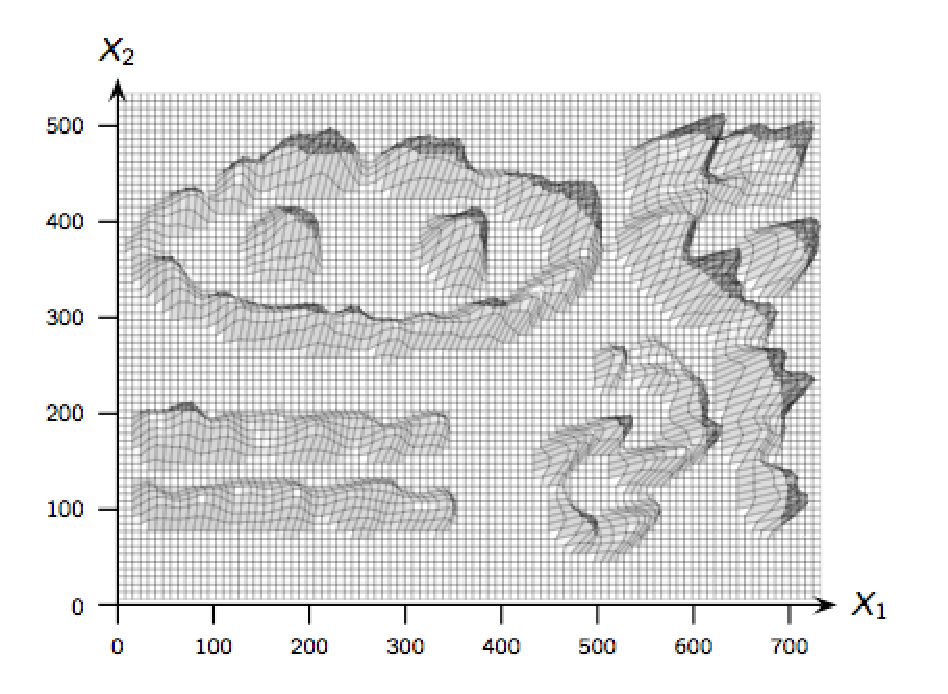
\includegraphics[scale=0.6]{CLUST/density/figs/draftfigs/denclueNCclusters.eps}
%%  }{
%%%\comment{%
%\psset{unit=0.5in}
%\psset{viewpoint=70 90 91 rtp2xyz,Decran=65}
%\psset{lightsrc=viewpoint}
%\psset{incolor=white}
%\psset{opacity=0.15}
%\begin{pspicture}(-1,-0.5)(7,6)
%\psset{fillcolor=white}
%\psSolid[object=objfile, file=CLUST/density/figs/t7-4k-h10-xi1.9surf,
%  transform={1 1 1.75 scaleOpoint3d},
%  linewidth=0.01pt,base=0 7.0 0 5.0]
%\psPoint(0,0,0){O2}
%\psPoint(7.5,0,0){X2}
%\psPoint(0,5.5,0){Y2}
%\psline[arrows=->,arrowscale=2](O2)(X2)
%\psline[arrows=->,arrowscale=2](O2)(Y2)
%\uput[r](X2){$X_1$}
%\uput[u](Y2){$X_2$}
%\psset{dotstyle=Bo,fillcolor=gray,linecolor=lightgray}
%\psset{dotsize=0.05}
%\psPoint(5.73663, 4.62705, 3.000000){p0}
\psdot(p0)
\psPoint(2.72958, 3.58739, 3.000000){p1}
\psdot(p1)
\psPoint(4.88711, 2.18802, 3.000000){p2}
\psdot(p2)
\psPoint(0.2647, 3.53756, 3.000000){p3}
\psdot(p3)
\psPoint(3.91275, 4.10433, 3.000000){p4}
\psdot(p4)
\psPoint(6.36726, 2.28562, 3.000000){p5}
\psdot(p5)
\psPoint(1.37104, 2.71697, 3.000000){p6}
\psdot(p6)
\psPoint(5.26954, 4.2366, 3.000000){p7}
\psdot(p7)
\psPoint(4.40992, 0.62826, 3.000000){p8}
\psdot(p8)
\psPoint(3.30697, 3.51166, 3.000000){p9}
\psdot(p9)
\psPoint(3.14221, 4.11265, 3.000000){p10}
\psdot(p10)
\psPoint(1.82901, 3.51725, 3.000000){p11}
\psdot(p11)
\psPoint(6.28531, 1.50092, 3.000000){p12}
\psdot(p12)
\psPoint(6.6524, 4.09595, 3.000000){p13}
\psdot(p13)
\psPoint(1.60336, 2.75217, 3.000000){p14}
\psdot(p14)
\psPoint(5.09416, 1.3411, 3.000000){p15}
\psdot(p15)
\psPoint(2.68271, 1.44971, 3.000000){p16}
\psdot(p16)
\psPoint(4.324, 3.88274, 3.000000){p17}
\psdot(p17)
\psPoint(3.10828, 4.04414, 3.000000){p18}
\psdot(p18)
\psPoint(6.22866, 3.28758, 3.000000){p19}
\psdot(p19)
\psPoint(5.60466, 3.53041, 3.000000){p20}
\psdot(p20)
\psPoint(5.35098, 4.57578, 3.000000){p21}
\psdot(p21)
\psPoint(1.62748, 3.6749, 3.000000){p22}
\psdot(p22)
\psPoint(2.28702, 1.04394, 3.000000){p23}
\psdot(p23)
\psPoint(5.33845, 1.23349, 3.000000){p24}
\psdot(p24)
\psPoint(6.25158, 2.4282, 3.000000){p25}
\psdot(p25)
\psPoint(1.94606, 2.60517, 3.000000){p26}
\psdot(p26)
\psPoint(3.13138, 3.04009, 3.000000){p27}
\psdot(p27)
\psPoint(1.34019, 2.82918, 3.000000){p28}
\psdot(p28)
\psPoint(5.63753, 2.31232, 3.000000){p29}
\psdot(p29)
\psPoint(6.10765, 2.15919, 3.000000){p30}
\psdot(p30)
\psPoint(4.20488, 2.78139, 3.000000){p31}
\psdot(p31)
\psPoint(2.7114, 3.45803, 3.000000){p32}
\psdot(p32)
\psPoint(6.38583, 3.6565, 3.000000){p33}
\psdot(p33)
\psPoint(3.27559, 1.11013, 3.000000){p34}
\psdot(p34)
\psPoint(1.47269, 1.83251, 3.000000){p35}
\psdot(p35)
\psPoint(6.29318, 4.52661, 3.000000){p36}
\psdot(p36)
\psPoint(2.00888, 1.6863, 3.000000){p37}
\psdot(p37)
\psPoint(2.76389, 1.63719, 3.000000){p38}
\psdot(p38)
\psPoint(2.2185, 4.40864, 3.000000){p39}
\psdot(p39)
\psPoint(1.06713, 1.58568, 3.000000){p40}
\psdot(p40)
\psPoint(3.14936, 3.24915, 3.000000){p41}
\psdot(p41)
\psPoint(3.77075, 4.2577, 3.000000){p42}
\psdot(p42)
\psPoint(6.74818, 3.24548, 3.000000){p43}
\psdot(p43)
\psPoint(4.98069, 2.45935, 3.000000){p44}
\psdot(p44)
\psPoint(5.08035, 2.15328, 3.000000){p45}
\psdot(p45)
\psPoint(1.2955, 3.45552, 3.000000){p46}
\psdot(p46)
\psPoint(3.19688, 3.6028, 3.000000){p47}
\psdot(p47)
\psPoint(1.6331, 3.52216, 3.000000){p48}
\psdot(p48)
\psPoint(0.79592, 0.76397, 3.000000){p49}
\psdot(p49)
\psPoint(4.01346, 2.78385, 3.000000){p50}
\psdot(p50)
\psPoint(2.72275, 4.45758, 3.000000){p51}
\psdot(p51)
\psPoint(3.45812, 2.72642, 3.000000){p52}
\psdot(p52)
\psPoint(4.65386, 2.11468, 3.000000){p53}
\psdot(p53)
\psPoint(1.50459, 2.37566, 3.000000){p54}
\psdot(p54)
\psPoint(0.55135, 3.82346, 3.000000){p55}
\psdot(p55)
\psPoint(2.71278, 3.3212, 3.000000){p56}
\psdot(p56)
\psPoint(3.65264, 2.61569, 3.000000){p57}
\psdot(p57)
\psPoint(5.52828, 3.04859, 3.000000){p58}
\psdot(p58)
\psPoint(6.09945, 1.58653, 3.000000){p59}
\psdot(p59)
\psPoint(1.42781, 3.16362, 3.000000){p60}
\psdot(p60)
\psPoint(2.53523, 4.32818, 3.000000){p61}
\psdot(p61)
\psPoint(2.21221, 3.44022, 3.000000){p62}
\psdot(p62)
\psPoint(1.95446, 2.59275, 3.000000){p63}
\psdot(p63)
\psPoint(6.6288, 1.14582, 3.000000){p64}
\psdot(p64)
\psPoint(3.22503, 1.37376, 3.000000){p65}
\psdot(p65)
\psPoint(2.63353, 4.04726, 3.000000){p66}
\psdot(p66)
\psPoint(1.7918, 2.79618, 3.000000){p67}
\psdot(p67)
\psPoint(2.26701, 2.43069, 3.000000){p68}
\psdot(p68)
\psPoint(2.01895, 4.21718, 3.000000){p69}
\psdot(p69)
\psPoint(2.49635, 1.47358, 3.000000){p70}
\psdot(p70)
\psPoint(0.33276, 1.12226, 3.000000){p71}
\psdot(p71)
\psPoint(4.90376, 0.60239, 3.000000){p72}
\psdot(p72)
\psPoint(6.43405, 2.36404, 3.000000){p73}
\psdot(p73)
\psPoint(1.79363, 3.43574, 3.000000){p74}
\psdot(p74)
\psPoint(2.37357, 1.79362, 3.000000){p75}
\psdot(p75)
\psPoint(5.7449, 1.53965, 3.000000){p76}
\psdot(p76)
\psPoint(4.21076, 3.21448, 3.000000){p77}
\psdot(p77)
\psPoint(3.64513, 3.30463, 3.000000){p78}
\psdot(p78)
\psPoint(2.4378, 0.99689, 3.000000){p79}
\psdot(p79)
\psPoint(4.07023, 4.15673, 3.000000){p80}
\psdot(p80)
\psPoint(1.4818, 0.7151, 3.000000){p81}
\psdot(p81)
\psPoint(6.60578, 1.18683, 3.000000){p82}
\psdot(p82)
\psPoint(2.1271, 1.80665, 3.000000){p83}
\psdot(p83)
\psPoint(2.83488, 1.00249, 3.000000){p84}
\psdot(p84)
\psPoint(1.69333, 0.98483, 3.000000){p85}
\psdot(p85)
\psPoint(5.96785, 3.95191, 3.000000){p86}
\psdot(p86)
\psPoint(2.92148, 3.02648, 3.000000){p87}
\psdot(p87)
\psPoint(2.43962, 4.40814, 3.000000){p88}
\psdot(p88)
\psPoint(0.26873, 1.70355, 3.000000){p89}
\psdot(p89)
\psPoint(0.22939, 0.88756, 3.000000){p90}
\psdot(p90)
\psPoint(3.42257, 3.05089, 3.000000){p91}
\psdot(p91)
\psPoint(0.7893, 2.78739, 3.000000){p92}
\psdot(p92)
\psPoint(6.41912, 0.69422, 3.000000){p93}
\psdot(p93)
\psPoint(3.35147, 3.14891, 3.000000){p94}
\psdot(p94)
\psPoint(1.93055, 4.36953, 3.000000){p95}
\psdot(p95)
\psPoint(3.65041, 2.72918, 3.000000){p96}
\psdot(p96)
\psPoint(0.40033, 0.74325, 3.000000){p97}
\psdot(p97)
\psPoint(0.54094, 0.6893, 3.000000){p98}
\psdot(p98)
\psPoint(1.98517, 0.97118, 3.000000){p99}
\psdot(p99)
\psPoint(3.30539, 1.64632, 3.000000){p100}
\psdot(p100)
\psPoint(4.23694, 1.3456, 3.000000){p101}
\psdot(p101)
\psPoint(1.91472, 3.47015, 3.000000){p102}
\psdot(p102)
\psPoint(2.20093, 4.15472, 3.000000){p103}
\psdot(p103)
\psPoint(6.23064, 3.5785, 3.000000){p104}
\psdot(p104)
\psPoint(1.70007, 2.65446, 3.000000){p105}
\psdot(p105)
\psPoint(1.24455, 4.15932, 3.000000){p106}
\psdot(p106)
\psPoint(6.43697, 2.3382, 3.000000){p107}
\psdot(p107)
\psPoint(0.66523, 2.83799, 3.000000){p108}
\psdot(p108)
\psPoint(0.92504, 2.66296, 3.000000){p109}
\psdot(p109)
\psPoint(6.07416, 1.88377, 3.000000){p110}
\psdot(p110)
\psPoint(2.82745, 2.46628, 3.000000){p111}
\psdot(p111)
\psPoint(5.57546, 1.83663, 3.000000){p112}
\psdot(p112)
\psPoint(2.76517, 4.05353, 3.000000){p113}
\psdot(p113)
\psPoint(3.01349, 1.5568, 3.000000){p114}
\psdot(p114)
\psPoint(2.45933, 2.47694, 3.000000){p115}
\psdot(p115)
\psPoint(6.28105, 3.47213, 3.000000){p116}
\psdot(p116)
\psPoint(6.3499, 4.49028, 3.000000){p117}
\psdot(p117)
\psPoint(4.73044, 1.693, 3.000000){p118}
\psdot(p118)
\psPoint(1.91319, 4.09425, 3.000000){p119}
\psdot(p119)
\psPoint(6.30689, 1.45696, 3.000000){p120}
\psdot(p120)
\psPoint(5.45515, 2.05062, 3.000000){p121}
\psdot(p121)
\psPoint(0.87172, 2.84134, 3.000000){p122}
\psdot(p122)
\psPoint(5.26582, 0.75995, 3.000000){p123}
\psdot(p123)
\psPoint(3.45197, 3.5103, 3.000000){p124}
\psdot(p124)
\psPoint(5.49355, 4.10475, 3.000000){p125}
\psdot(p125)
\psPoint(4.12013, 2.73039, 3.000000){p126}
\psdot(p126)
\psPoint(0.75356, 1.0483, 3.000000){p127}
\psdot(p127)
\psPoint(1.62154, 1.12124, 3.000000){p128}
\psdot(p128)
\psPoint(2.23541, 2.58017, 3.000000){p129}
\psdot(p129)
\psPoint(5.55218, 1.55698, 3.000000){p130}
\psdot(p130)
\psPoint(0.68767, 2.1258, 3.000000){p131}
\psdot(p131)
\psPoint(5.05604, 0.80587, 3.000000){p132}
\psdot(p132)
\psPoint(2.55987, 4.15031, 3.000000){p133}
\psdot(p133)
\psPoint(3.54939, 1.31378, 3.000000){p134}
\psdot(p134)
\psPoint(4.93986, 4.52359, 3.000000){p135}
\psdot(p135)
\psPoint(2.95339, 1.61434, 3.000000){p136}
\psdot(p136)
\psPoint(4.23311, 2.01298, 3.000000){p137}
\psdot(p137)
\psPoint(3.19884, 3.13587, 3.000000){p138}
\psdot(p138)
\psPoint(4.74385, 1.66211, 3.000000){p139}
\psdot(p139)
\psPoint(6.39365, 1.63731, 3.000000){p140}
\psdot(p140)
\psPoint(5.16499, 1.19602, 3.000000){p141}
\psdot(p141)
\psPoint(5.48895, 3.53427, 3.000000){p142}
\psdot(p142)
\psPoint(6.31181, 0.90578, 3.000000){p143}
\psdot(p143)
\psPoint(5.31025, 4.09594, 3.000000){p144}
\psdot(p144)
\psPoint(1.92684, 4.13771, 3.000000){p145}
\psdot(p145)
\psPoint(1.26147, 4.26478, 3.000000){p146}
\psdot(p146)
\psPoint(0.63907, 3.71659, 3.000000){p147}
\psdot(p147)
\psPoint(4.33522, 3.8791, 3.000000){p148}
\psdot(p148)
\psPoint(0.2488, 1.78809, 3.000000){p149}
\psdot(p149)
\psPoint(2.80907, 0.75983, 3.000000){p150}
\psdot(p150)
\psPoint(2.34124, 2.693, 3.000000){p151}
\psdot(p151)
\psPoint(1.18043, 2.68763, 3.000000){p152}
\psdot(p152)
\psPoint(1.33566, 3.24192, 3.000000){p153}
\psdot(p153)
\psPoint(1.24917, 4.16612, 3.000000){p154}
\psdot(p154)
\psPoint(1.35319, 1.82999, 3.000000){p155}
\psdot(p155)
\psPoint(1.85582, 1.59981, 3.000000){p156}
\psdot(p156)
\psPoint(4.72289, 1.70258, 3.000000){p157}
\psdot(p157)
\psPoint(4.38462, 3.28804, 3.000000){p158}
\psdot(p158)
\psPoint(3.1386, 3.74769, 3.000000){p159}
\psdot(p159)
\psPoint(1.57031, 1.38417, 3.000000){p160}
\psdot(p160)
\psPoint(3.57676, 3.14311, 3.000000){p161}
\psdot(p161)
\psPoint(1.56265, 0.40148, 3.000000){p162}
\psdot(p162)
\psPoint(1.3951, 3.6332, 3.000000){p163}
\psdot(p163)
\psPoint(1.13792, 3.89306, 3.000000){p164}
\psdot(p164)
\psPoint(0.65201, 4.00415, 3.000000){p165}
\psdot(p165)
\psPoint(0.44926, 3.0539, 3.000000){p166}
\psdot(p166)
\psPoint(5.58751, 4.16916, 3.000000){p167}
\psdot(p167)
\psPoint(6.05976, 2.1104, 3.000000){p168}
\psdot(p168)
\psPoint(6.02285, 3.7345, 3.000000){p169}
\psdot(p169)
\psPoint(1.32272, 3.1766, 3.000000){p170}
\psdot(p170)
\psPoint(1.71561, 2.8003, 3.000000){p171}
\psdot(p171)
\psPoint(6.01888, 4.37302, 3.000000){p172}
\psdot(p172)
\psPoint(4.51057, 1.47524, 3.000000){p173}
\psdot(p173)
\psPoint(4.63561, 0.83951, 3.000000){p174}
\psdot(p174)
\psPoint(1.57916, 1.92259, 3.000000){p175}
\psdot(p175)
\psPoint(0.82632, 0.90993, 3.000000){p176}
\psdot(p176)
\psPoint(0.40363, 1.72293, 3.000000){p177}
\psdot(p177)
\psPoint(6.06236, 2.20902, 3.000000){p178}
\psdot(p178)
\psPoint(3.68392, 4.11804, 3.000000){p179}
\psdot(p179)
\psPoint(5.33909, 4.47317, 3.000000){p180}
\psdot(p180)
\psPoint(5.82308, 4.31827, 3.000000){p181}
\psdot(p181)
\psPoint(1.84201, 2.71984, 3.000000){p182}
\psdot(p182)
\psPoint(6.26318, 3.2178, 3.000000){p183}
\psdot(p183)
\psPoint(0.65152, 0.87445, 3.000000){p184}
\psdot(p184)
\psPoint(5.67278, 4.00157, 3.000000){p185}
\psdot(p185)
\psPoint(1.6136, 1.58388, 3.000000){p186}
\psdot(p186)
\psPoint(3.16973, 4.29696, 3.000000){p187}
\psdot(p187)
\psPoint(2.09105, 4.33396, 3.000000){p188}
\psdot(p188)
\psPoint(4.72407, 3.62644, 3.000000){p189}
\psdot(p189)
\psPoint(6.23942, 2.42762, 3.000000){p190}
\psdot(p190)
\psPoint(5.88914, 3.13694, 3.000000){p191}
\psdot(p191)
\psPoint(6.44574, 1.09599, 3.000000){p192}
\psdot(p192)
\psPoint(6.83215, 3.28168, 3.000000){p193}
\psdot(p193)
\psPoint(6.01327, 4.17243, 3.000000){p194}
\psdot(p194)
\psPoint(5.0772, 3.54306, 3.000000){p195}
\psdot(p195)
\psPoint(2.54236, 0.84097, 3.000000){p196}
\psdot(p196)
\psPoint(6.25616, 1.96519, 3.000000){p197}
\psdot(p197)
\psPoint(0.43105, 3.5388, 3.000000){p198}
\psdot(p198)
\psPoint(6.52831, 2.0227, 3.000000){p199}
\psdot(p199)
\psPoint(4.93472, 1.72017, 3.000000){p200}
\psdot(p200)
\psPoint(0.75768, 3.86666, 3.000000){p201}
\psdot(p201)
\psPoint(6.71685, 3.6448, 3.000000){p202}
\psdot(p202)
\psPoint(6.26168, 3.25358, 3.000000){p203}
\psdot(p203)
\psPoint(2.16678, 0.52878, 3.000000){p204}
\psdot(p204)
\psPoint(5.16723, 1.39649, 3.000000){p205}
\psdot(p205)
\psPoint(0.31262, 2.27115, 3.000000){p206}
\psdot(p206)
\psPoint(5.22584, 1.07244, 3.000000){p207}
\psdot(p207)
\psPoint(2.01416, 1.63788, 3.000000){p208}
\psdot(p208)
\psPoint(3.77341, 2.59234, 3.000000){p209}
\psdot(p209)
\psPoint(4.74275, 2.27441, 3.000000){p210}
\psdot(p210)
\psPoint(1.59964, 1.3839, 3.000000){p211}
\psdot(p211)
\psPoint(0.69485, 1.10585, 3.000000){p212}
\psdot(p212)
\psPoint(4.5654, 3.02206, 3.000000){p213}
\psdot(p213)
\psPoint(3.45122, 2.81928, 3.000000){p214}
\psdot(p214)
\psPoint(5.09961, 0.88616, 3.000000){p215}
\psdot(p215)
\psPoint(3.37224, 4.34136, 3.000000){p216}
\psdot(p216)
\psPoint(4.12508, 3.97621, 3.000000){p217}
\psdot(p217)
\psPoint(0.7401, 0.73671, 3.000000){p218}
\psdot(p218)
\psPoint(5.36621, 4.48563, 3.000000){p219}
\psdot(p219)
\psPoint(1.43467, 4.25734, 3.000000){p220}
\psdot(p220)
\psPoint(4.26936, 3.83646, 3.000000){p221}
\psdot(p221)
\psPoint(0.98283, 1.02789, 3.000000){p222}
\psdot(p222)
\psPoint(5.50675, 3.27448, 3.000000){p223}
\psdot(p223)
\psPoint(1.87395, 1.52099, 3.000000){p224}
\psdot(p224)
\psPoint(3.38582, 3.97027, 3.000000){p225}
\psdot(p225)
\psPoint(1.99447, 0.91465, 3.000000){p226}
\psdot(p226)
\psPoint(0.55245, 0.77925, 3.000000){p227}
\psdot(p227)
\psPoint(5.64601, 3.66443, 3.000000){p228}
\psdot(p228)
\psPoint(5.30758, 3.38816, 3.000000){p229}
\psdot(p229)
\psPoint(6.6143, 3.72276, 3.000000){p230}
\psdot(p230)
\psPoint(6.33869, 1.88259, 3.000000){p231}
\psdot(p231)
\psPoint(0.80111, 1.56644, 3.000000){p232}
\psdot(p232)
\psPoint(3.74516, 3.01581, 3.000000){p233}
\psdot(p233)
\psPoint(5.67845, 4.14547, 3.000000){p234}
\psdot(p234)
\psPoint(5.54264, 2.99127, 3.000000){p235}
\psdot(p235)
\psPoint(1.68283, 2.5795, 3.000000){p236}
\psdot(p236)
\psPoint(1.58359, 1.11598, 3.000000){p237}
\psdot(p237)
\psPoint(1.28238, 4.29041, 3.000000){p238}
\psdot(p238)
\psPoint(4.56452, 0.70104, 3.000000){p239}
\psdot(p239)
\psPoint(1.9673, 2.63448, 3.000000){p240}
\psdot(p240)
\psPoint(1.0041, 0.97905, 3.000000){p241}
\psdot(p241)
\psPoint(5.75176, 1.53382, 3.000000){p242}
\psdot(p242)
\psPoint(5.52192, 4.23151, 3.000000){p243}
\psdot(p243)
\psPoint(2.17973, 1.70295, 3.000000){p244}
\psdot(p244)
\psPoint(0.25923, 0.70788, 3.000000){p245}
\psdot(p245)
\psPoint(6.05508, 2.25926, 3.000000){p246}
\psdot(p246)
\psPoint(4.41551, 3.4523, 3.000000){p247}
\psdot(p247)
\psPoint(5.47195, 4.24432, 3.000000){p248}
\psdot(p248)
\psPoint(1.67199, 2.5512, 3.000000){p249}
\psdot(p249)
\psPoint(2.30877, 4.36569, 3.000000){p250}
\psdot(p250)
\psPoint(0.58391, 3.14439, 3.000000){p251}
\psdot(p251)
\psPoint(3.24897, 2.62238, 3.000000){p252}
\psdot(p252)
\psPoint(6.2659, 2.25893, 3.000000){p253}
\psdot(p253)
\psPoint(6.6, 4.47613, 3.000000){p254}
\psdot(p254)
\psPoint(0.43668, 2.91399, 3.000000){p255}
\psdot(p255)
\psPoint(6.73834, 4.35254, 3.000000){p256}
\psdot(p256)
\psPoint(1.04347, 1.75611, 3.000000){p257}
\psdot(p257)
\psPoint(3.17203, 1.06982, 3.000000){p258}
\psdot(p258)
\psPoint(0.63116, 3.69837, 3.000000){p259}
\psdot(p259)
\psPoint(1.56759, 4.00334, 3.000000){p260}
\psdot(p260)
\psPoint(6.30543, 2.66906, 3.000000){p261}
\psdot(p261)
\psPoint(0.50432, 2.99391, 3.000000){p262}
\psdot(p262)
\psPoint(5.17639, 4.20626, 3.000000){p263}
\psdot(p263)
\psPoint(6.50768, 3.47282, 3.000000){p264}
\psdot(p264)
\psPoint(1.65121, 3.45513, 3.000000){p265}
\psdot(p265)
\psPoint(5.34698, 3.63307, 3.000000){p266}
\psdot(p266)
\psPoint(6.40128, 1.95589, 3.000000){p267}
\psdot(p267)
\psPoint(6.07945, 2.87715, 3.000000){p268}
\psdot(p268)
\psPoint(2.49584, 1.40167, 3.000000){p269}
\psdot(p269)
\psPoint(4.90302, 0.50079, 3.000000){p270}
\psdot(p270)
\psPoint(5.15194, 2.2245, 3.000000){p271}
\psdot(p271)
\psPoint(2.06045, 4.36023, 3.000000){p272}
\psdot(p272)
\psPoint(6.32503, 3.33636, 3.000000){p273}
\psdot(p273)
\psPoint(3.58222, 3.39086, 3.000000){p274}
\psdot(p274)
\psPoint(3.51077, 3.15341, 3.000000){p275}
\psdot(p275)
\psPoint(2.69046, 4.15209, 3.000000){p276}
\psdot(p276)
\psPoint(5.35199, 3.80906, 3.000000){p277}
\psdot(p277)
\psPoint(6.36148, 4.22864, 3.000000){p278}
\psdot(p278)
\psPoint(0.36111, 2.99347, 3.000000){p279}
\psdot(p279)
\psPoint(0.71835, 4.68426, 3.000000){p280}
\psdot(p280)
\psPoint(2.7267, 0.49079, 3.000000){p281}
\psdot(p281)
\psPoint(1.7103, 4.03242, 3.000000){p282}
\psdot(p282)
\psPoint(0.97422, 2.24053, 3.000000){p283}
\psdot(p283)
\psPoint(0.21128, 3.11598, 3.000000){p284}
\psdot(p284)
\psPoint(1.68941, 1.65506, 3.000000){p285}
\psdot(p285)
\psPoint(6.45005, 1.67336, 3.000000){p286}
\psdot(p286)
\psPoint(2.81878, 4.07031, 3.000000){p287}
\psdot(p287)
\psPoint(6.39466, 3.12162, 3.000000){p288}
\psdot(p288)
\psPoint(6.47406, 1.65395, 3.000000){p289}
\psdot(p289)
\psPoint(3.79223, 2.72997, 3.000000){p290}
\psdot(p290)
\psPoint(6.59622, 3.03381, 3.000000){p291}
\psdot(p291)
\psPoint(4.63956, 3.5492, 3.000000){p292}
\psdot(p292)
\psPoint(4.72749, 1.4843, 3.000000){p293}
\psdot(p293)
\psPoint(2.72765, 3.40341, 3.000000){p294}
\psdot(p294)
\psPoint(5.77438, 2.69242, 3.000000){p295}
\psdot(p295)
\psPoint(0.69475, 1.7223, 3.000000){p296}
\psdot(p296)
\psPoint(6.09168, 2.4507, 3.000000){p297}
\psdot(p297)
\psPoint(3.37386, 4.21004, 3.000000){p298}
\psdot(p298)
\psPoint(2.20006, 4.32739, 3.000000){p299}
\psdot(p299)
\psPoint(4.48146, 3.93502, 3.000000){p300}
\psdot(p300)
\psPoint(3.30506, 1.32799, 3.000000){p301}
\psdot(p301)
\psPoint(2.37464, 4.26733, 3.000000){p302}
\psdot(p302)
\psPoint(5.36556, 4.17417, 3.000000){p303}
\psdot(p303)
\psPoint(3.20408, 0.71723, 3.000000){p304}
\psdot(p304)
\psPoint(2.8883, 1.41494, 3.000000){p305}
\psdot(p305)
\psPoint(0.55153, 3.81593, 3.000000){p306}
\psdot(p306)
\psPoint(4.93319, 1.3526, 3.000000){p307}
\psdot(p307)
\psPoint(2.07055, 4.27265, 3.000000){p308}
\psdot(p308)
\psPoint(5.49898, 1.82936, 3.000000){p309}
\psdot(p309)
\psPoint(6.7724, 1.71324, 3.000000){p310}
\psdot(p310)
\psPoint(5.27402, 3.94848, 3.000000){p311}
\psdot(p311)
\psPoint(4.82287, 0.72297, 3.000000){p312}
\psdot(p312)
\psPoint(5.12532, 2.48172, 3.000000){p313}
\psdot(p313)
\psPoint(6.55928, 3.31411, 3.000000){p314}
\psdot(p314)
\psPoint(6.38076, 3.95519, 3.000000){p315}
\psdot(p315)
\psPoint(6.42192, 1.18147, 3.000000){p316}
\psdot(p316)
\psPoint(2.93233, 2.73559, 3.000000){p317}
\psdot(p317)
\psPoint(1.16626, 2.98558, 3.000000){p318}
\psdot(p318)
\psPoint(5.45988, 4.37964, 3.000000){p319}
\psdot(p319)
\psPoint(0.61127, 0.9923, 3.000000){p320}
\psdot(p320)
\psPoint(0.67919, 1.83032, 3.000000){p321}
\psdot(p321)
\psPoint(4.46962, 3.24436, 3.000000){p322}
\psdot(p322)
\psPoint(0.54469, 3.21346, 3.000000){p323}
\psdot(p323)
\psPoint(4.44529, 3.76501, 3.000000){p324}
\psdot(p324)
\psPoint(5.44441, 4.46594, 3.000000){p325}
\psdot(p325)
\psPoint(3.78167, 2.64315, 3.000000){p326}
\psdot(p326)
\psPoint(4.3546, 3.48163, 3.000000){p327}
\psdot(p327)
\psPoint(6.88904, 4.00265, 3.000000){p328}
\psdot(p328)
\psPoint(5.32918, 1.29125, 3.000000){p329}
\psdot(p329)
\psPoint(5.68816, 4.43492, 3.000000){p330}
\psdot(p330)
\psPoint(5.57338, 2.99815, 3.000000){p331}
\psdot(p331)
\psPoint(6.4714, 1.08757, 3.000000){p332}
\psdot(p332)
\psPoint(3.38683, 3.45399, 3.000000){p333}
\psdot(p333)
\psPoint(1.87419, 0.79655, 3.000000){p334}
\psdot(p334)
\psPoint(0.97908, 2.33809, 3.000000){p335}
\psdot(p335)
\psPoint(3.31139, 2.70079, 3.000000){p336}
\psdot(p336)
\psPoint(5.93909, 2.52438, 3.000000){p337}
\psdot(p337)
\psPoint(4.47242, 1.45226, 3.000000){p338}
\psdot(p338)
\psPoint(0.18958, 3.71422, 3.000000){p339}
\psdot(p339)
\psPoint(3.88146, 3.86002, 3.000000){p340}
\psdot(p340)
\psPoint(1.02495, 0.76782, 3.000000){p341}
\psdot(p341)
\psPoint(6.79437, 3.21916, 3.000000){p342}
\psdot(p342)
\psPoint(1.07186, 1.09662, 3.000000){p343}
\psdot(p343)
\psPoint(6.66254, 3.66738, 3.000000){p344}
\psdot(p344)
\psPoint(6.26247, 1.92001, 3.000000){p345}
\psdot(p345)
\psPoint(5.43797, 1.53217, 3.000000){p346}
\psdot(p346)
\psPoint(6.14086, 2.82568, 3.000000){p347}
\psdot(p347)
\psPoint(0.57621, 2.04114, 3.000000){p348}
\psdot(p348)
\psPoint(0.3171, 4.52782, 3.000000){p349}
\psdot(p349)
\psPoint(5.59704, 1.3375, 3.000000){p350}
\psdot(p350)
\psPoint(1.76827, 2.71573, 3.000000){p351}
\psdot(p351)
\psPoint(1.76387, 1.00872, 3.000000){p352}
\psdot(p352)
\psPoint(6.3339, 2.715, 3.000000){p353}
\psdot(p353)
\psPoint(0.76498, 1.6303, 3.000000){p354}
\psdot(p354)
\psPoint(5.3748, 3.72144, 3.000000){p355}
\psdot(p355)
\psPoint(1.96603, 0.99323, 3.000000){p356}
\psdot(p356)
\psPoint(2.30875, 2.47045, 3.000000){p357}
\psdot(p357)
\psPoint(6.32893, 4.4226, 3.000000){p358}
\psdot(p358)
\psPoint(1.19811, 1.63209, 3.000000){p359}
\psdot(p359)
\psPoint(6.20745, 2.09016, 3.000000){p360}
\psdot(p360)
\psPoint(0.52893, 3.16242, 3.000000){p361}
\psdot(p361)
\psPoint(6.31171, 1.6361, 3.000000){p362}
\psdot(p362)
\psPoint(5.66964, 2.93507, 3.000000){p363}
\psdot(p363)
\psPoint(5.06381, 0.55863, 3.000000){p364}
\psdot(p364)
\psPoint(3.4449, 3.38303, 3.000000){p365}
\psdot(p365)
\psPoint(6.75318, 1.35111, 3.000000){p366}
\psdot(p366)
\psPoint(2.51272, 1.69212, 3.000000){p367}
\psdot(p367)
\psPoint(2.56228, 2.67487, 3.000000){p368}
\psdot(p368)
\psPoint(4.29008, 1.47643, 3.000000){p369}
\psdot(p369)
\psPoint(4.79218, 1.53336, 3.000000){p370}
\psdot(p370)
\psPoint(0.83149, 4.13325, 3.000000){p371}
\psdot(p371)
\psPoint(2.98536, 4.40791, 3.000000){p372}
\psdot(p372)
\psPoint(3.03881, 2.84747, 3.000000){p373}
\psdot(p373)
\psPoint(5.16818, 3.43442, 3.000000){p374}
\psdot(p374)
\psPoint(5.15267, 4.29652, 3.000000){p375}
\psdot(p375)
\psPoint(6.39284, 1.5542, 3.000000){p376}
\psdot(p376)
\psPoint(0.19915, 1.63184, 3.000000){p377}
\psdot(p377)
\psPoint(1.18478, 3.89856, 3.000000){p378}
\psdot(p378)
\psPoint(1.5081, 4.27675, 3.000000){p379}
\psdot(p379)
\psPoint(2.83176, 0.81482, 3.000000){p380}
\psdot(p380)
\psPoint(5.10104, 1.17978, 3.000000){p381}
\psdot(p381)
\psPoint(1.07398, 0.92721, 3.000000){p382}
\psdot(p382)
\psPoint(5.60184, 1.9229, 3.000000){p383}
\psdot(p383)
\psPoint(1.60661, 0.77249, 3.000000){p384}
\psdot(p384)
\psPoint(5.05899, 4.30419, 3.000000){p385}
\psdot(p385)
\psPoint(6.1764, 4.41848, 3.000000){p386}
\psdot(p386)
\psPoint(5.80608, 2.97477, 3.000000){p387}
\psdot(p387)
\psPoint(1.94471, 1.57387, 3.000000){p388}
\psdot(p388)
\psPoint(0.52852, 0.51333, 3.000000){p389}
\psdot(p389)
\psPoint(4.37, 1.12594, 3.000000){p390}
\psdot(p390)
\psPoint(0.96668, 3.26076, 3.000000){p391}
\psdot(p391)
\psPoint(6.42616, 3.91003, 3.000000){p392}
\psdot(p392)
\psPoint(5.23712, 0.75024, 3.000000){p393}
\psdot(p393)
\psPoint(1.68784, 2.50097, 3.000000){p394}
\psdot(p394)
\psPoint(1.53696, 1.83013, 3.000000){p395}
\psdot(p395)
\psPoint(1.83649, 0.69686, 3.000000){p396}
\psdot(p396)
\psPoint(3.15706, 3.71246, 3.000000){p397}
\psdot(p397)
\psPoint(5.51177, 1.3499, 3.000000){p398}
\psdot(p398)
\psPoint(3.42967, 3.14769, 3.000000){p399}
\psdot(p399)
\psPoint(5.64464, 2.92351, 3.000000){p400}
\psdot(p400)
\psPoint(6.34972, 2.68941, 3.000000){p401}
\psdot(p401)
\psPoint(4.12059, 3.90992, 3.000000){p402}
\psdot(p402)
\psPoint(6.66425, 4.0301, 3.000000){p403}
\psdot(p403)
\psPoint(2.1278, 4.19444, 3.000000){p404}
\psdot(p404)
\psPoint(5.24047, 0.7332, 3.000000){p405}
\psdot(p405)
\psPoint(3.40544, 2.59696, 3.000000){p406}
\psdot(p406)
\psPoint(2.6691, 2.47372, 3.000000){p407}
\psdot(p407)
\psPoint(1.52039, 3.47884, 3.000000){p408}
\psdot(p408)
\psPoint(3.19237, 2.35704, 3.000000){p409}
\psdot(p409)
\psPoint(5.52761, 3.6918, 3.000000){p410}
\psdot(p410)
\psPoint(1.90534, 1.71928, 3.000000){p411}
\psdot(p411)
\psPoint(6.16671, 1.578, 3.000000){p412}
\psdot(p412)
\psPoint(5.8499, 4.01861, 3.000000){p413}
\psdot(p413)
\psPoint(1.82346, 0.9309, 3.000000){p414}
\psdot(p414)
\psPoint(1.9209, 1.6004, 3.000000){p415}
\psdot(p415)
\psPoint(2.35531, 1.72255, 3.000000){p416}
\psdot(p416)
\psPoint(2.87187, 1.94975, 3.000000){p417}
\psdot(p417)
\psPoint(4.3555, 1.45395, 3.000000){p418}
\psdot(p418)
\psPoint(1.53756, 2.66591, 3.000000){p419}
\psdot(p419)
\psPoint(2.3782, 1.68025, 3.000000){p420}
\psdot(p420)
\psPoint(3.1944, 2.87986, 3.000000){p421}
\psdot(p421)
\psPoint(3.36544, 3.78734, 3.000000){p422}
\psdot(p422)
\psPoint(1.64317, 3.3597, 3.000000){p423}
\psdot(p423)
\psPoint(5.82839, 2.48324, 3.000000){p424}
\psdot(p424)
\psPoint(5.79467, 4.00796, 3.000000){p425}
\psdot(p425)
\psPoint(4.31691, 1.61683, 3.000000){p426}
\psdot(p426)
\psPoint(3.1086, 0.7664, 3.000000){p427}
\psdot(p427)
\psPoint(2.11731, 1.71762, 3.000000){p428}
\psdot(p428)
\psPoint(1.28739, 3.47509, 3.000000){p429}
\psdot(p429)
\psPoint(6.65525, 3.11745, 3.000000){p430}
\psdot(p430)
\psPoint(6.51605, 4.33026, 3.000000){p431}
\psdot(p431)
\psPoint(6.15035, 2.80036, 3.000000){p432}
\psdot(p432)
\psPoint(1.20956, 4.06173, 3.000000){p433}
\psdot(p433)
\psPoint(0.2925, 1.10994, 3.000000){p434}
\psdot(p434)
\psPoint(6.46799, 1.97472, 3.000000){p435}
\psdot(p435)
\psPoint(1.96022, 2.50524, 3.000000){p436}
\psdot(p436)
\psPoint(2.59747, 1.02947, 3.000000){p437}
\psdot(p437)
\psPoint(5.35119, 3.28844, 3.000000){p438}
\psdot(p438)
\psPoint(2.54791, 1.68611, 3.000000){p439}
\psdot(p439)
\psPoint(5.5737, 3.82783, 3.000000){p440}
\psdot(p440)
\psPoint(5.52675, 1.60487, 3.000000){p441}
\psdot(p441)
\psPoint(3.69659, 3.64719, 3.000000){p442}
\psdot(p442)
\psPoint(2.40717, 1.78755, 3.000000){p443}
\psdot(p443)
\psPoint(0.49992, 1.51781, 3.000000){p444}
\psdot(p444)
\psPoint(1.61942, 1.07855, 3.000000){p445}
\psdot(p445)
\psPoint(6.6158, 4.65583, 3.000000){p446}
\psdot(p446)
\psPoint(0.96318, 3.22427, 3.000000){p447}
\psdot(p447)
\psPoint(5.45841, 3.57713, 3.000000){p448}
\psdot(p448)
\psPoint(0.40876, 1.39333, 3.000000){p449}
\psdot(p449)
\psPoint(3.29793, 2.57679, 3.000000){p450}
\psdot(p450)
\psPoint(0.91366, 3.81387, 3.000000){p451}
\psdot(p451)
\psPoint(3.0401, 3.27502, 3.000000){p452}
\psdot(p452)
\psPoint(3.61669, 1.10422, 3.000000){p453}
\psdot(p453)
\psPoint(1.29035, 0.75443, 3.000000){p454}
\psdot(p454)
\psPoint(2.8277, 2.48761, 3.000000){p455}
\psdot(p455)
\psPoint(5.98192, 2.62925, 3.000000){p456}
\psdot(p456)
\psPoint(3.14091, 3.33808, 3.000000){p457}
\psdot(p457)
\psPoint(1.15486, 1.77085, 3.000000){p458}
\psdot(p458)
\psPoint(4.21075, 1.23893, 3.000000){p459}
\psdot(p459)
\psPoint(0.61395, 0.77725, 3.000000){p460}
\psdot(p460)
\psPoint(2.7912, 4.12833, 3.000000){p461}
\psdot(p461)
\psPoint(5.56709, 3.16791, 3.000000){p462}
\psdot(p462)
\psPoint(1.1673, 2.66861, 3.000000){p463}
\psdot(p463)
\psPoint(0.30821, 3.11726, 3.000000){p464}
\psdot(p464)
\psPoint(5.4545, 1.37991, 3.000000){p465}
\psdot(p465)
\psPoint(5.512, 2.94298, 3.000000){p466}
\psdot(p466)
\psPoint(1.75568, 3.53932, 3.000000){p467}
\psdot(p467)
\psPoint(2.18038, 4.24521, 3.000000){p468}
\psdot(p468)
\psPoint(6.11727, 2.64127, 3.000000){p469}
\psdot(p469)
\psPoint(1.33514, 1.45516, 3.000000){p470}
\psdot(p470)
\psPoint(4.92417, 3.69676, 3.000000){p471}
\psdot(p471)
\psPoint(3.73137, 1.2193, 3.000000){p472}
\psdot(p472)
\psPoint(2.40801, 1.81178, 3.000000){p473}
\psdot(p473)
\psPoint(6.42546, 4.07835, 3.000000){p474}
\psdot(p474)
\psPoint(1.28583, 0.81599, 3.000000){p475}
\psdot(p475)
\psPoint(5.71178, 4.34044, 3.000000){p476}
\psdot(p476)
\psPoint(0.96868, 0.88464, 3.000000){p477}
\psdot(p477)
\psPoint(3.83731, 2.81223, 3.000000){p478}
\psdot(p478)
\psPoint(1.69409, 4.1367, 3.000000){p479}
\psdot(p479)
\psPoint(0.65527, 1.61731, 3.000000){p480}
\psdot(p480)
\psPoint(3.81522, 3.86891, 3.000000){p481}
\psdot(p481)
\psPoint(5.39512, 4.11975, 3.000000){p482}
\psdot(p482)
\psPoint(4.20737, 1.34844, 3.000000){p483}
\psdot(p483)
\psPoint(3.31648, 1.00469, 3.000000){p484}
\psdot(p484)
\psPoint(3.18721, 4.25091, 3.000000){p485}
\psdot(p485)
\psPoint(4.22267, 1.01899, 3.000000){p486}
\psdot(p486)
\psPoint(4.46698, 3.73311, 3.000000){p487}
\psdot(p487)
\psPoint(1.34177, 3.32106, 3.000000){p488}
\psdot(p488)
\psPoint(0.61427, 1.38457, 3.000000){p489}
\psdot(p489)
\psPoint(4.82255, 0.82785, 3.000000){p490}
\psdot(p490)
\psPoint(6.55832, 3.15994, 3.000000){p491}
\psdot(p491)
\psPoint(3.16302, 4.05178, 3.000000){p492}
\psdot(p492)
\psPoint(2.60292, 2.44799, 3.000000){p493}
\psdot(p493)
\psPoint(3.192, 3.99345, 3.000000){p494}
\psdot(p494)
\psPoint(2.17336, 3.15332, 3.000000){p495}
\psdot(p495)
\psPoint(4.8061, 2.12461, 3.000000){p496}
\psdot(p496)
\psPoint(1.57373, 4.5159, 3.000000){p497}
\psdot(p497)
\psPoint(5.73764, 1.61152, 3.000000){p498}
\psdot(p498)
\psPoint(1.49663, 0.83439, 3.000000){p499}
\psdot(p499)
\psPoint(0.90712, 3.40385, 3.000000){p500}
\psdot(p500)
\psPoint(4.92166, 0.86233, 3.000000){p501}
\psdot(p501)
\psPoint(5.44398, 2.02037, 3.000000){p502}
\psdot(p502)
\psPoint(6.38116, 3.64046, 3.000000){p503}
\psdot(p503)
\psPoint(5.26802, 0.96915, 3.000000){p504}
\psdot(p504)
\psPoint(4.79296, 2.31044, 3.000000){p505}
\psdot(p505)
\psPoint(5.50772, 3.03124, 3.000000){p506}
\psdot(p506)
\psPoint(0.06321, 3.85885, 3.000000){p507}
\psdot(p507)
\psPoint(6.37969, 2.11983, 3.000000){p508}
\psdot(p508)
\psPoint(6.61636, 3.20209, 3.000000){p509}
\psdot(p509)
\psPoint(5.28344, 2.23133, 3.000000){p510}
\psdot(p510)
\psPoint(5.28569, 1.21502, 3.000000){p511}
\psdot(p511)
\psPoint(0.33045, 1.82992, 3.000000){p512}
\psdot(p512)
\psPoint(5.40385, 3.73822, 3.000000){p513}
\psdot(p513)
\psPoint(3.0895, 1.57438, 3.000000){p514}
\psdot(p514)
\psPoint(5.35456, 0.87448, 3.000000){p515}
\psdot(p515)
\psPoint(0.29557, 4.57349, 3.000000){p516}
\psdot(p516)
\psPoint(0.94842, 1.35204, 3.000000){p517}
\psdot(p517)
\psPoint(1.06489, 1.09052, 3.000000){p518}
\psdot(p518)
\psPoint(5.76499, 1.96431, 3.000000){p519}
\psdot(p519)
\psPoint(5.55071, 4.27039, 3.000000){p520}
\psdot(p520)
\psPoint(2.4882, 1.4489, 3.000000){p521}
\psdot(p521)
\psPoint(2.16684, 3.47716, 3.000000){p522}
\psdot(p522)
\psPoint(1.7395, 4.32248, 3.000000){p523}
\psdot(p523)
\psPoint(3.82863, 3.86952, 3.000000){p524}
\psdot(p524)
\psPoint(5.66947, 1.79118, 3.000000){p525}
\psdot(p525)
\psPoint(3.9211, 2.70973, 3.000000){p526}
\psdot(p526)
\psPoint(5.50336, 2.88853, 3.000000){p527}
\psdot(p527)
\psPoint(6.21649, 2.20381, 3.000000){p528}
\psdot(p528)
\psPoint(4.69035, 1.55808, 3.000000){p529}
\psdot(p529)
\psPoint(2.402, 1.01601, 3.000000){p530}
\psdot(p530)
\psPoint(0.41348, 0.84674, 3.000000){p531}
\psdot(p531)
\psPoint(1.54658, 2.78778, 3.000000){p532}
\psdot(p532)
\psPoint(3.74334, 2.75758, 3.000000){p533}
\psdot(p533)
\psPoint(5.45743, 1.22257, 3.000000){p534}
\psdot(p534)
\psPoint(6.76582, 4.37993, 3.000000){p535}
\psdot(p535)
\psPoint(1.0806, 0.52495, 3.000000){p536}
\psdot(p536)
\psPoint(6.5088, 0.79186, 3.000000){p537}
\psdot(p537)
\psPoint(6.05158, 3.94075, 3.000000){p538}
\psdot(p538)
\psPoint(5.0002, 1.3852, 3.000000){p539}
\psdot(p539)
\psPoint(1.79202, 3.46054, 3.000000){p540}
\psdot(p540)
\psPoint(5.60799, 1.36883, 3.000000){p541}
\psdot(p541)
\psPoint(6.07244, 1.64625, 3.000000){p542}
\psdot(p542)
\psPoint(6.42695, 3.85322, 3.000000){p543}
\psdot(p543)
\psPoint(0.51149, 0.85005, 3.000000){p544}
\psdot(p544)
\psPoint(5.59646, 4.32453, 3.000000){p545}
\psdot(p545)
\psPoint(5.57014, 3.86488, 3.000000){p546}
\psdot(p546)
\psPoint(0.71418, 3.82115, 3.000000){p547}
\psdot(p547)
\psPoint(1.31744, 1.78142, 3.000000){p548}
\psdot(p548)
\psPoint(5.39051, 3.74546, 3.000000){p549}
\psdot(p549)
\psPoint(5.81416, 4.07668, 3.000000){p550}
\psdot(p550)
\psPoint(4.49833, 3.81645, 3.000000){p551}
\psdot(p551)
\psPoint(4.57278, 3.49225, 3.000000){p552}
\psdot(p552)
\psPoint(0.76857, 4.20646, 3.000000){p553}
\psdot(p553)
\psPoint(4.42001, 1.33891, 3.000000){p554}
\psdot(p554)
\psPoint(4.32295, 1.87368, 3.000000){p555}
\psdot(p555)
\psPoint(4.35737, 2.9331, 3.000000){p556}
\psdot(p556)
\psPoint(5.2378, 3.53627, 3.000000){p557}
\psdot(p557)
\psPoint(4.4533, 1.63444, 3.000000){p558}
\psdot(p558)
\psPoint(0.69422, 3.11279, 3.000000){p559}
\psdot(p559)
\psPoint(5.04326, 4.03652, 3.000000){p560}
\psdot(p560)
\psPoint(1.19403, 2.87875, 3.000000){p561}
\psdot(p561)
\psPoint(3.67699, 1.42716, 3.000000){p562}
\psdot(p562)
\psPoint(3.67515, 2.58701, 3.000000){p563}
\psdot(p563)
\psPoint(1.43297, 1.45345, 3.000000){p564}
\psdot(p564)
\psPoint(5.65667, 2.93317, 3.000000){p565}
\psdot(p565)
\psPoint(6.27924, 2.03328, 3.000000){p566}
\psdot(p566)
\psPoint(1.7074, 4.66536, 3.000000){p567}
\psdot(p567)
\psPoint(2.01689, 0.92804, 3.000000){p568}
\psdot(p568)
\psPoint(0.40666, 0.82996, 3.000000){p569}
\psdot(p569)
\psPoint(1.50739, 0.91307, 3.000000){p570}
\psdot(p570)
\psPoint(5.32814, 2.96114, 3.000000){p571}
\psdot(p571)
\psPoint(4.30754, 3.87635, 3.000000){p572}
\psdot(p572)
\psPoint(6.53362, 4.45377, 3.000000){p573}
\psdot(p573)
\psPoint(4.23813, 3.41303, 3.000000){p574}
\psdot(p574)
\psPoint(5.31421, 4.30824, 3.000000){p575}
\psdot(p575)
\psPoint(3.8383, 3.98269, 3.000000){p576}
\psdot(p576)
\psPoint(1.75907, 1.00194, 3.000000){p577}
\psdot(p577)
\psPoint(1.8429, 3.33656, 3.000000){p578}
\psdot(p578)
\psPoint(2.41581, 1.06008, 3.000000){p579}
\psdot(p579)
\psPoint(4.26709, 1.25924, 3.000000){p580}
\psdot(p580)
\psPoint(5.59568, 3.08893, 3.000000){p581}
\psdot(p581)
\psPoint(0.97632, 2.4605, 3.000000){p582}
\psdot(p582)
\psPoint(6.87922, 3.40661, 3.000000){p583}
\psdot(p583)
\psPoint(1.16218, 1.00384, 3.000000){p584}
\psdot(p584)
\psPoint(4.00747, 3.90309, 3.000000){p585}
\psdot(p585)
\psPoint(3.53844, 3.1388, 3.000000){p586}
\psdot(p586)
\psPoint(0.46813, 3.52385, 3.000000){p587}
\psdot(p587)
\psPoint(4.27567, 4.03036, 3.000000){p588}
\psdot(p588)
\psPoint(4.44593, 1.02186, 3.000000){p589}
\psdot(p589)
\psPoint(5.50384, 1.39181, 3.000000){p590}
\psdot(p590)
\psPoint(0.66539, 1.7091, 3.000000){p591}
\psdot(p591)
\psPoint(6.35719, 1.61542, 3.000000){p592}
\psdot(p592)
\psPoint(1.75103, 1.10701, 3.000000){p593}
\psdot(p593)
\psPoint(1.55747, 0.93085, 3.000000){p594}
\psdot(p594)
\psPoint(2.57065, 1.03918, 3.000000){p595}
\psdot(p595)
\psPoint(4.8486, 2.28521, 3.000000){p596}
\psdot(p596)
\psPoint(4.34419, 3.01307, 3.000000){p597}
\psdot(p597)
\psPoint(5.25257, 3.21555, 3.000000){p598}
\psdot(p598)
\psPoint(4.50007, 2.04032, 3.000000){p599}
\psdot(p599)
\psPoint(0.28521, 3.01506, 3.000000){p600}
\psdot(p600)
\psPoint(2.89827, 0.92748, 3.000000){p601}
\psdot(p601)
\psPoint(6.57124, 4.50481, 3.000000){p602}
\psdot(p602)
\psPoint(5.00674, 0.7016, 3.000000){p603}
\psdot(p603)
\psPoint(6.57496, 1.13951, 3.000000){p604}
\psdot(p604)
\psPoint(3.02103, 4.21332, 3.000000){p605}
\psdot(p605)
\psPoint(2.71065, 2.87122, 3.000000){p606}
\psdot(p606)
\psPoint(5.8455, 3.98314, 3.000000){p607}
\psdot(p607)
\psPoint(5.51726, 3.58382, 3.000000){p608}
\psdot(p608)
\psPoint(3.4667, 4.13496, 3.000000){p609}
\psdot(p609)
\psPoint(1.51764, 3.46701, 3.000000){p610}
\psdot(p610)
\psPoint(2.05575, 4.10898, 3.000000){p611}
\psdot(p611)
\psPoint(2.29634, 4.13161, 3.000000){p612}
\psdot(p612)
\psPoint(5.74776, 1.49666, 3.000000){p613}
\psdot(p613)
\psPoint(1.16118, 2.70099, 3.000000){p614}
\psdot(p614)
\psPoint(2.67887, 4.03794, 3.000000){p615}
\psdot(p615)
\psPoint(1.31309, 2.64388, 3.000000){p616}
\psdot(p616)
\psPoint(6.52603, 4.49103, 3.000000){p617}
\psdot(p617)
\psPoint(0.32332, 0.96076, 3.000000){p618}
\psdot(p618)
\psPoint(4.96425, 3.76623, 3.000000){p619}
\psdot(p619)
\psPoint(5.37073, 3.43324, 3.000000){p620}
\psdot(p620)
\psPoint(4.96519, 2.31653, 3.000000){p621}
\psdot(p621)
\psPoint(1.35242, 2.64538, 3.000000){p622}
\psdot(p622)
\psPoint(0.59543, 0.89465, 3.000000){p623}
\psdot(p623)
\psPoint(6.59022, 1.47444, 3.000000){p624}
\psdot(p624)
\psPoint(5.3248, 3.16115, 3.000000){p625}
\psdot(p625)
\psPoint(0.43204, 3.55895, 3.000000){p626}
\psdot(p626)
\psPoint(1.44907, 1.13889, 3.000000){p627}
\psdot(p627)
\psPoint(3.61789, 3.49989, 3.000000){p628}
\psdot(p628)
\psPoint(1.47506, 2.60899, 3.000000){p629}
\psdot(p629)
\psPoint(5.52415, 4.40576, 3.000000){p630}
\psdot(p630)
\psPoint(3.19244, 1.60797, 3.000000){p631}
\psdot(p631)
\psPoint(6.14355, 4.47963, 3.000000){p632}
\psdot(p632)
\psPoint(5.28132, 3.57187, 3.000000){p633}
\psdot(p633)
\psPoint(3.65356, 1.41425, 3.000000){p634}
\psdot(p634)
\psPoint(0.31623, 3.26346, 3.000000){p635}
\psdot(p635)
\psPoint(5.33045, 0.34978, 3.000000){p636}
\psdot(p636)
\psPoint(6.36304, 4.4411, 3.000000){p637}
\psdot(p637)
\psPoint(0.30392, 1.80353, 3.000000){p638}
\psdot(p638)
\psPoint(6.39311, 3.14082, 3.000000){p639}
\psdot(p639)
\psPoint(6.01816, 4.46305, 3.000000){p640}
\psdot(p640)
\psPoint(0.82642, 1.7122, 3.000000){p641}
\psdot(p641)
\psPoint(6.29966, 1.18034, 3.000000){p642}
\psdot(p642)
\psPoint(0.79632, 3.94409, 3.000000){p643}
\psdot(p643)
\psPoint(4.5452, 1.45119, 3.000000){p644}
\psdot(p644)
\psPoint(2.86177, 3.42244, 3.000000){p645}
\psdot(p645)
\psPoint(4.4457, 1.01574, 3.000000){p646}
\psdot(p646)
\psPoint(4.76422, 3.42458, 3.000000){p647}
\psdot(p647)
\psPoint(0.48979, 3.23149, 3.000000){p648}
\psdot(p648)
\psPoint(4.05399, 4.07597, 3.000000){p649}
\psdot(p649)
\psPoint(5.58439, 4.12091, 3.000000){p650}
\psdot(p650)
\psPoint(2.76824, 2.53898, 3.000000){p651}
\psdot(p651)
\psPoint(1.44523, 2.76057, 3.000000){p652}
\psdot(p652)
\psPoint(6.36046, 1.81612, 3.000000){p653}
\psdot(p653)
\psPoint(6.43814, 0.70362, 3.000000){p654}
\psdot(p654)
\psPoint(6.55635, 4.27006, 3.000000){p655}
\psdot(p655)
\psPoint(6.40049, 1.09364, 3.000000){p656}
\psdot(p656)
\psPoint(3.29534, 1.76617, 3.000000){p657}
\psdot(p657)
\psPoint(6.49368, 4.2945, 3.000000){p658}
\psdot(p658)
\psPoint(6.05055, 0.65335, 3.000000){p659}
\psdot(p659)
\psPoint(5.69496, 4.03554, 3.000000){p660}
\psdot(p660)
\psPoint(1.24793, 3.48795, 3.000000){p661}
\psdot(p661)
\psPoint(3.19796, 2.74158, 3.000000){p662}
\psdot(p662)
\psPoint(6.47759, 1.20481, 3.000000){p663}
\psdot(p663)
\psPoint(2.24667, 1.44896, 3.000000){p664}
\psdot(p664)
\psPoint(4.23173, 1.23604, 3.000000){p665}
\psdot(p665)
\psPoint(6.59654, 4.00335, 3.000000){p666}
\psdot(p666)
\psPoint(5.27298, 1.3736, 3.000000){p667}
\psdot(p667)
\psPoint(5.59947, 3.44313, 3.000000){p668}
\psdot(p668)
\psPoint(1.59167, 3.61297, 3.000000){p669}
\psdot(p669)
\psPoint(1.17998, 4.00035, 3.000000){p670}
\psdot(p670)
\psPoint(5.88882, 3.01082, 3.000000){p671}
\psdot(p671)
\psPoint(5.49795, 1.66147, 3.000000){p672}
\psdot(p672)
\psPoint(3.77427, 2.77387, 3.000000){p673}
\psdot(p673)
\psPoint(1.83097, 3.21517, 3.000000){p674}
\psdot(p674)
\psPoint(4.26128, 2.86682, 3.000000){p675}
\psdot(p675)
\psPoint(5.25329, 4.08777, 3.000000){p676}
\psdot(p676)
\psPoint(3.01913, 0.76552, 3.000000){p677}
\psdot(p677)
\psPoint(4.23152, 1.20814, 3.000000){p678}
\psdot(p678)
\psPoint(6.66064, 2.63011, 3.000000){p679}
\psdot(p679)
\psPoint(0.57476, 1.75723, 3.000000){p680}
\psdot(p680)
\psPoint(5.00822, 0.75995, 3.000000){p681}
\psdot(p681)
\psPoint(0.70221, 3.80266, 3.000000){p682}
\psdot(p682)
\psPoint(6.49167, 0.74495, 3.000000){p683}
\psdot(p683)
\psPoint(5.18364, 2.51864, 3.000000){p684}
\psdot(p684)
\psPoint(1.33326, 3.61271, 3.000000){p685}
\psdot(p685)
\psPoint(1.98015, 4.30943, 3.000000){p686}
\psdot(p686)
\psPoint(4.50642, 0.70156, 3.000000){p687}
\psdot(p687)
\psPoint(6.68443, 3.58913, 3.000000){p688}
\psdot(p688)
\psPoint(2.86745, 4.73703, 3.000000){p689}
\psdot(p689)
\psPoint(3.13351, 0.68931, 3.000000){p690}
\psdot(p690)
\psPoint(5.25345, 2.49365, 3.000000){p691}
\psdot(p691)
\psPoint(1.56341, 4.58145, 3.000000){p692}
\psdot(p692)
\psPoint(1.00617, 1.59144, 3.000000){p693}
\psdot(p693)
\psPoint(6.14358, 1.5489, 3.000000){p694}
\psdot(p694)
\psPoint(5.70648, 4.62232, 3.000000){p695}
\psdot(p695)
\psPoint(5.49128, 1.94162, 3.000000){p696}
\psdot(p696)
\psPoint(2.85811, 2.50394, 3.000000){p697}
\psdot(p697)
\psPoint(6.19945, 2.8301, 3.000000){p698}
\psdot(p698)
\psPoint(4.32953, 2.89514, 3.000000){p699}
\psdot(p699)
\psPoint(1.0521, 2.86344, 3.000000){p700}
\psdot(p700)
\psPoint(5.05913, 1.38923, 3.000000){p701}
\psdot(p701)
\psPoint(5.06913, 4.0126, 3.000000){p702}
\psdot(p702)
\psPoint(0.75864, 3.70152, 3.000000){p703}
\psdot(p703)
\psPoint(6.12123, 1.63035, 3.000000){p704}
\psdot(p704)
\psPoint(6.24851, 3.18255, 3.000000){p705}
\psdot(p705)
\psPoint(2.34878, 1.81878, 3.000000){p706}
\psdot(p706)
\psPoint(6.22039, 2.12251, 3.000000){p707}
\psdot(p707)
\psPoint(5.94091, 4.59856, 3.000000){p708}
\psdot(p708)
\psPoint(2.20416, 2.56351, 3.000000){p709}
\psdot(p709)
\psPoint(6.18088, 1.85987, 3.000000){p710}
\psdot(p710)
\psPoint(2.84823, 4.33442, 3.000000){p711}
\psdot(p711)
\psPoint(2.93698, 1.74443, 3.000000){p712}
\psdot(p712)
\psPoint(2.06036, 2.75737, 3.000000){p713}
\psdot(p713)
\psPoint(4.67237, 1.63015, 3.000000){p714}
\psdot(p714)
\psPoint(3.28447, 3.19295, 3.000000){p715}
\psdot(p715)
\psPoint(5.98466, 3.75537, 3.000000){p716}
\psdot(p716)
\psPoint(6.44647, 3.25905, 3.000000){p717}
\psdot(p717)
\psPoint(1.91965, 4.08839, 3.000000){p718}
\psdot(p718)
\psPoint(3.1142, 1.44999, 3.000000){p719}
\psdot(p719)
\psPoint(2.94912, 4.2148, 3.000000){p720}
\psdot(p720)
\psPoint(6.56827, 1.70574, 3.000000){p721}
\psdot(p721)
\psPoint(0.4691, 0.93008, 3.000000){p722}
\psdot(p722)
\psPoint(5.30934, 0.91579, 3.000000){p723}
\psdot(p723)
\psPoint(3.29298, 3.07033, 3.000000){p724}
\psdot(p724)
\psPoint(2.96876, 4.26281, 3.000000){p725}
\psdot(p725)
\psPoint(5.92573, 2.7324, 3.000000){p726}
\psdot(p726)
\psPoint(5.27397, 0.75471, 3.000000){p727}
\psdot(p727)
\psPoint(3.53396, 3.2917, 3.000000){p728}
\psdot(p728)
\psPoint(1.44614, 3.20949, 3.000000){p729}
\psdot(p729)
\psPoint(1.83617, 3.52579, 3.000000){p730}
\psdot(p730)
\psPoint(6.03032, 4.44463, 3.000000){p731}
\psdot(p731)
\psPoint(0.9233, 3.95157, 3.000000){p732}
\psdot(p732)
\psPoint(3.18265, 1.5948, 3.000000){p733}
\psdot(p733)
\psPoint(0.38135, 0.81592, 3.000000){p734}
\psdot(p734)
\psPoint(4.87203, 1.55054, 3.000000){p735}
\psdot(p735)
\psPoint(4.52694, 0.58149, 3.000000){p736}
\psdot(p736)
\psPoint(1.53739, 4.04411, 3.000000){p737}
\psdot(p737)
\psPoint(4.41856, 1.66512, 3.000000){p738}
\psdot(p738)
\psPoint(2.16846, 4.11747, 3.000000){p739}
\psdot(p739)
\psPoint(4.96164, 4.4876, 3.000000){p740}
\psdot(p740)
\psPoint(1.48744, 1.38274, 3.000000){p741}
\psdot(p741)
\psPoint(0.65715, 2.93322, 3.000000){p742}
\psdot(p742)
\psPoint(5.57209, 3.09862, 3.000000){p743}
\psdot(p743)
\psPoint(4.11151, 3.14535, 3.000000){p744}
\psdot(p744)
\psPoint(0.66619, 1.67592, 3.000000){p745}
\psdot(p745)
\psPoint(2.86909, 1.54986, 3.000000){p746}
\psdot(p746)
\psPoint(6.37791, 3.50903, 3.000000){p747}
\psdot(p747)
\psPoint(1.52194, 1.53153, 3.000000){p748}
\psdot(p748)
\psPoint(3.37823, 3.23939, 3.000000){p749}
\psdot(p749)
\psPoint(5.04598, 1.24781, 3.000000){p750}
\psdot(p750)
\psPoint(1.64079, 0.91507, 3.000000){p751}
\psdot(p751)
\psPoint(2.37855, 2.45505, 3.000000){p752}
\psdot(p752)
\psPoint(2.58925, 2.6552, 3.000000){p753}
\psdot(p753)
\psPoint(0.21409, 1.81389, 3.000000){p754}
\psdot(p754)
\psPoint(3.26708, 0.76465, 3.000000){p755}
\psdot(p755)
\psPoint(1.88622, 4.17373, 3.000000){p756}
\psdot(p756)
\psPoint(3.45674, 3.40309, 3.000000){p757}
\psdot(p757)
\psPoint(4.28716, 2.79232, 3.000000){p758}
\psdot(p758)
\psPoint(5.88628, 1.81076, 3.000000){p759}
\psdot(p759)
\psPoint(0.74503, 0.78407, 3.000000){p760}
\psdot(p760)
\psPoint(5.30117, 2.53398, 3.000000){p761}
\psdot(p761)
\psPoint(4.33571, 4.01859, 3.000000){p762}
\psdot(p762)
\psPoint(0.77671, 3.87262, 3.000000){p763}
\psdot(p763)
\psPoint(3.69011, 2.93706, 3.000000){p764}
\psdot(p764)
\psPoint(1.58873, 3.04666, 3.000000){p765}
\psdot(p765)
\psPoint(5.43882, 3.19738, 3.000000){p766}
\psdot(p766)
\psPoint(4.90389, 0.46649, 3.000000){p767}
\psdot(p767)
\psPoint(5.32055, 1.22724, 3.000000){p768}
\psdot(p768)
\psPoint(6.5611, 1.36136, 3.000000){p769}
\psdot(p769)
\psPoint(2.76786, 1.16775, 3.000000){p770}
\psdot(p770)
\psPoint(6.15194, 2.1984, 3.000000){p771}
\psdot(p771)
\psPoint(5.12456, 4.16987, 3.000000){p772}
\psdot(p772)
\psPoint(5.51222, 1.01063, 3.000000){p773}
\psdot(p773)
\psPoint(5.14144, 1.29276, 3.000000){p774}
\psdot(p774)
\psPoint(2.57264, 1.42807, 3.000000){p775}
\psdot(p775)
\psPoint(4.47146, 3.56751, 3.000000){p776}
\psdot(p776)
\psPoint(2.16791, 1.46862, 3.000000){p777}
\psdot(p777)
\psPoint(0.91282, 3.81058, 3.000000){p778}
\psdot(p778)
\psPoint(6.11899, 2.12694, 3.000000){p779}
\psdot(p779)
\psPoint(1.67942, 4.09219, 3.000000){p780}
\psdot(p780)
\psPoint(6.64394, 3.32123, 3.000000){p781}
\psdot(p781)
\psPoint(6.52268, 3.26389, 3.000000){p782}
\psdot(p782)
\psPoint(4.82757, 1.80824, 3.000000){p783}
\psdot(p783)
\psPoint(3.25985, 4.32681, 3.000000){p784}
\psdot(p784)
\psPoint(6.27604, 1.29176, 3.000000){p785}
\psdot(p785)
\psPoint(1.63388, 1.76343, 3.000000){p786}
\psdot(p786)
\psPoint(5.6316, 3.52825, 3.000000){p787}
\psdot(p787)
\psPoint(1.46538, 2.73415, 3.000000){p788}
\psdot(p788)
\psPoint(4.81873, 3.38631, 3.000000){p789}
\psdot(p789)
\psPoint(5.32113, 1.31972, 3.000000){p790}
\psdot(p790)
\psPoint(6.08123, 1.54255, 3.000000){p791}
\psdot(p791)
\psPoint(5.63396, 1.54952, 3.000000){p792}
\psdot(p792)
\psPoint(1.75986, 1.05128, 3.000000){p793}
\psdot(p793)
\psPoint(6.42441, 0.65103, 3.000000){p794}
\psdot(p794)
\psPoint(6.56534, 1.27134, 3.000000){p795}
\psdot(p795)
\psPoint(2.61788, 2.53575, 3.000000){p796}
\psdot(p796)
\psPoint(2.37209, 0.72019, 3.000000){p797}
\psdot(p797)
\psPoint(4.47426, 0.58319, 3.000000){p798}
\psdot(p798)
\psPoint(5.56316, 3.95302, 3.000000){p799}
\psdot(p799)
\psPoint(1.98407, 1.72213, 3.000000){p800}
\psdot(p800)
\psPoint(1.53593, 4.09775, 3.000000){p801}
\psdot(p801)
\psPoint(0.63834, 4.07371, 3.000000){p802}
\psdot(p802)
\psPoint(4.31532, 3.06559, 3.000000){p803}
\psdot(p803)
\psPoint(5.56326, 4.36638, 3.000000){p804}
\psdot(p804)
\psPoint(1.62707, 3.46898, 3.000000){p805}
\psdot(p805)
\psPoint(3.1537, 4.18724, 3.000000){p806}
\psdot(p806)
\psPoint(5.70371, 3.02122, 3.000000){p807}
\psdot(p807)
\psPoint(2.83933, 2.58991, 3.000000){p808}
\psdot(p808)
\psPoint(1.84005, 3.42395, 3.000000){p809}
\psdot(p809)
\psPoint(6.00902, 2.13196, 3.000000){p810}
\psdot(p810)
\psPoint(6.1494, 1.55577, 3.000000){p811}
\psdot(p811)
\psPoint(1.07594, 1.09229, 3.000000){p812}
\psdot(p812)
\psPoint(2.11704, 4.17878, 3.000000){p813}
\psdot(p813)
\psPoint(1.67426, 2.80525, 3.000000){p814}
\psdot(p814)
\psPoint(1.27008, 1.04615, 3.000000){p815}
\psdot(p815)
\psPoint(3.1549, 1.69066, 3.000000){p816}
\psdot(p816)
\psPoint(5.59383, 4.57334, 3.000000){p817}
\psdot(p817)
\psPoint(3.17621, 1.08413, 3.000000){p818}
\psdot(p818)
\psPoint(1.88619, 2.75365, 3.000000){p819}
\psdot(p819)
\psPoint(3.21477, 3.33909, 3.000000){p820}
\psdot(p820)
\psPoint(1.52451, 2.67613, 3.000000){p821}
\psdot(p821)
\psPoint(2.16693, 0.90176, 3.000000){p822}
\psdot(p822)
\psPoint(2.76967, 0.78989, 3.000000){p823}
\psdot(p823)
\psPoint(2.46713, 0.80096, 3.000000){p824}
\psdot(p824)
\psPoint(5.28138, 3.46492, 3.000000){p825}
\psdot(p825)
\psPoint(6.327, 3.68714, 3.000000){p826}
\psdot(p826)
\psPoint(6.83671, 4.22505, 3.000000){p827}
\psdot(p827)
\psPoint(4.84636, 2.43159, 3.000000){p828}
\psdot(p828)
\psPoint(0.30176, 1.63656, 3.000000){p829}
\psdot(p829)
\psPoint(2.71912, 3.21331, 3.000000){p830}
\psdot(p830)
\psPoint(5.57054, 4.10817, 3.000000){p831}
\psdot(p831)
\psPoint(4.35467, 0.73685, 3.000000){p832}
\psdot(p832)
\psPoint(2.28441, 3.4455, 3.000000){p833}
\psdot(p833)
\psPoint(2.17426, 3.87318, 3.000000){p834}
\psdot(p834)
\psPoint(1.26953, 1.53559, 3.000000){p835}
\psdot(p835)
\psPoint(5.66252, 3.76006, 3.000000){p836}
\psdot(p836)
\psPoint(6.17815, 2.25705, 3.000000){p837}
\psdot(p837)
\psPoint(6.68907, 4.12209, 3.000000){p838}
\psdot(p838)
\psPoint(3.07329, 3.40702, 3.000000){p839}
\psdot(p839)
\psPoint(4.5791, 3.79863, 3.000000){p840}
\psdot(p840)
\psPoint(0.67589, 3.69547, 3.000000){p841}
\psdot(p841)
\psPoint(0.37978, 3.77388, 3.000000){p842}
\psdot(p842)
\psPoint(0.21172, 3.1183, 3.000000){p843}
\psdot(p843)
\psPoint(6.37833, 1.88871, 3.000000){p844}
\psdot(p844)
\psPoint(2.35506, 4.05515, 3.000000){p845}
\psdot(p845)
\psPoint(5.25361, 4.19164, 3.000000){p846}
\psdot(p846)
\psPoint(1.44734, 1.04077, 3.000000){p847}
\psdot(p847)
\psPoint(6.42662, 2.45097, 3.000000){p848}
\psdot(p848)
\psPoint(5.40005, 3.77291, 3.000000){p849}
\psdot(p849)
\psPoint(3.05408, 0.95636, 3.000000){p850}
\psdot(p850)
\psPoint(6.75424, 3.2736, 3.000000){p851}
\psdot(p851)
\psPoint(5.58038, 3.24983, 3.000000){p852}
\psdot(p852)
\psPoint(6.37532, 3.13834, 3.000000){p853}
\psdot(p853)
\psPoint(4.47206, 3.06404, 3.000000){p854}
\psdot(p854)
\psPoint(1.90424, 0.69633, 3.000000){p855}
\psdot(p855)
\psPoint(2.58957, 1.69696, 3.000000){p856}
\psdot(p856)
\psPoint(5.54716, 4.60908, 3.000000){p857}
\psdot(p857)
\psPoint(6.29853, 0.9401, 3.000000){p858}
\psdot(p858)
\psPoint(5.27799, 1.38094, 3.000000){p859}
\psdot(p859)
\psPoint(4.87054, 2.43987, 3.000000){p860}
\psdot(p860)
\psPoint(0.39921, 0.9883, 3.000000){p861}
\psdot(p861)
\psPoint(4.87975, 0.7636, 3.000000){p862}
\psdot(p862)
\psPoint(3.22678, 0.77383, 3.000000){p863}
\psdot(p863)
\psPoint(4.25781, 0.29153, 3.000000){p864}
\psdot(p864)
\psPoint(3.92596, 3.16426, 3.000000){p865}
\psdot(p865)
\psPoint(2.07764, 4.08547, 3.000000){p866}
\psdot(p866)
\psPoint(1.23494, 4.04996, 3.000000){p867}
\psdot(p867)
\psPoint(1.95333, 1.46657, 3.000000){p868}
\psdot(p868)
\psPoint(3.27187, 3.05099, 3.000000){p869}
\psdot(p869)
\psPoint(2.87369, 4.34236, 3.000000){p870}
\psdot(p870)
\psPoint(0.47486, 2.10742, 3.000000){p871}
\psdot(p871)
\psPoint(0.96504, 0.55868, 3.000000){p872}
\psdot(p872)
\psPoint(0.06615, 3.55303, 3.000000){p873}
\psdot(p873)
\psPoint(1.61047, 1.67032, 3.000000){p874}
\psdot(p874)
\psPoint(5.15737, 3.54633, 3.000000){p875}
\psdot(p875)
\psPoint(4.21536, 3.64617, 3.000000){p876}
\psdot(p876)
\psPoint(0.46922, 3.98243, 3.000000){p877}
\psdot(p877)
\psPoint(5.88979, 4.03193, 3.000000){p878}
\psdot(p878)
\psPoint(5.57708, 1.43808, 3.000000){p879}
\psdot(p879)
\psPoint(1.30682, 2.81235, 3.000000){p880}
\psdot(p880)
\psPoint(1.84803, 2.75142, 3.000000){p881}
\psdot(p881)
\psPoint(5.24403, 1.31164, 3.000000){p882}
\psdot(p882)
\psPoint(2.95781, 2.63856, 3.000000){p883}
\psdot(p883)
\psPoint(6.07867, 2.57979, 3.000000){p884}
\psdot(p884)
\psPoint(2.61427, 4.67022, 3.000000){p885}
\psdot(p885)
\psPoint(4.8771, 2.14871, 3.000000){p886}
\psdot(p886)
\psPoint(6.5452, 3.73348, 3.000000){p887}
\psdot(p887)
\psPoint(1.27508, 3.50465, 3.000000){p888}
\psdot(p888)
\psPoint(2.03609, 1.39329, 3.000000){p889}
\psdot(p889)
\psPoint(0.37202, 1.42505, 3.000000){p890}
\psdot(p890)
\psPoint(3.3992, 3.20062, 3.000000){p891}
\psdot(p891)
\psPoint(1.42129, 4.19989, 3.000000){p892}
\psdot(p892)
\psPoint(6.51528, 1.38403, 3.000000){p893}
\psdot(p893)
\psPoint(6.32028, 1.94416, 3.000000){p894}
\psdot(p894)
\psPoint(2.21758, 4.23955, 3.000000){p895}
\psdot(p895)
\psPoint(4.00397, 3.97984, 3.000000){p896}
\psdot(p896)
\psPoint(5.03446, 0.73822, 3.000000){p897}
\psdot(p897)
\psPoint(1.93906, 4.07432, 3.000000){p898}
\psdot(p898)
\psPoint(0.71044, 3.02361, 3.000000){p899}
\psdot(p899)
\psPoint(3.74592, 1.63363, 3.000000){p900}
\psdot(p900)
\psPoint(6.28267, 2.79041, 3.000000){p901}
\psdot(p901)
\psPoint(5.07252, 3.54371, 3.000000){p902}
\psdot(p902)
\psPoint(0.94282, 1.4146, 3.000000){p903}
\psdot(p903)
\psPoint(6.57466, 2.47026, 3.000000){p904}
\psdot(p904)
\psPoint(2.56789, 1.51176, 3.000000){p905}
\psdot(p905)
\psPoint(2.77793, 4.31339, 3.000000){p906}
\psdot(p906)
\psPoint(3.36079, 2.6817, 3.000000){p907}
\psdot(p907)
\psPoint(2.6251, 4.19787, 3.000000){p908}
\psdot(p908)
\psPoint(6.28711, 0.28784, 3.000000){p909}
\psdot(p909)
\psPoint(1.51897, 3.24572, 3.000000){p910}
\psdot(p910)
\psPoint(2.00716, 2.13211, 3.000000){p911}
\psdot(p911)
\psPoint(0.45494, 3.03983, 3.000000){p912}
\psdot(p912)
\psPoint(4.87795, 2.38763, 3.000000){p913}
\psdot(p913)
\psPoint(5.85417, 1.5412, 3.000000){p914}
\psdot(p914)
\psPoint(1.0601, 2.6313, 3.000000){p915}
\psdot(p915)
\psPoint(3.35777, 3.26621, 3.000000){p916}
\psdot(p916)
\psPoint(3.04774, 4.08915, 3.000000){p917}
\psdot(p917)
\psPoint(1.11538, 1.09217, 3.000000){p918}
\psdot(p918)
\psPoint(3.7635, 0.67433, 3.000000){p919}
\psdot(p919)
\psPoint(5.72426, 4.62511, 3.000000){p920}
\psdot(p920)
\psPoint(5.32994, 4.09718, 3.000000){p921}
\psdot(p921)
\psPoint(5.18369, 0.85695, 3.000000){p922}
\psdot(p922)
\psPoint(5.92434, 2.71299, 3.000000){p923}
\psdot(p923)
\psPoint(0.64744, 1.58331, 3.000000){p924}
\psdot(p924)
\psPoint(3.41817, 0.6224, 3.000000){p925}
\psdot(p925)
\psPoint(4.93284, 1.29613, 3.000000){p926}
\psdot(p926)
\psPoint(2.55053, 4.3603, 3.000000){p927}
\psdot(p927)
\psPoint(0.35547, 0.71589, 3.000000){p928}
\psdot(p928)
\psPoint(1.22636, 1.05828, 3.000000){p929}
\psdot(p929)
\psPoint(6.34382, 1.33032, 3.000000){p930}
\psdot(p930)
\psPoint(6.56563, 1.79591, 3.000000){p931}
\psdot(p931)
\psPoint(5.21398, 3.36101, 3.000000){p932}
\psdot(p932)
\psPoint(4.77011, 0.43279, 3.000000){p933}
\psdot(p933)
\psPoint(4.58212, 3.25358, 3.000000){p934}
\psdot(p934)
\psPoint(2.54687, 2.56323, 3.000000){p935}
\psdot(p935)
\psPoint(1.78396, 0.81042, 3.000000){p936}
\psdot(p936)
\psPoint(2.28015, 4.38665, 3.000000){p937}
\psdot(p937)
\psPoint(0.35912, 3.7035, 3.000000){p938}
\psdot(p938)
\psPoint(2.93566, 4.36723, 3.000000){p939}
\psdot(p939)
\psPoint(0.31363, 1.62284, 3.000000){p940}
\psdot(p940)
\psPoint(1.21241, 4.16651, 3.000000){p941}
\psdot(p941)
\psPoint(1.11323, 2.71555, 3.000000){p942}
\psdot(p942)
\psPoint(2.07339, 1.74492, 3.000000){p943}
\psdot(p943)
\psPoint(1.5631, 4.30868, 3.000000){p944}
\psdot(p944)
\psPoint(0.95789, 4.14043, 3.000000){p945}
\psdot(p945)
\psPoint(0.32958, 1.47888, 3.000000){p946}
\psdot(p946)
\psPoint(3.14755, 3.74811, 3.000000){p947}
\psdot(p947)
\psPoint(1.11488, 3.93995, 3.000000){p948}
\psdot(p948)
\psPoint(4.56418, 1.26358, 3.000000){p949}
\psdot(p949)
\psPoint(5.26977, 3.29825, 3.000000){p950}
\psdot(p950)
\psPoint(1.41819, 1.07016, 3.000000){p951}
\psdot(p951)
\psPoint(6.49211, 3.12963, 3.000000){p952}
\psdot(p952)
\psPoint(4.31754, 3.78545, 3.000000){p953}
\psdot(p953)
\psPoint(1.86734, 3.40229, 3.000000){p954}
\psdot(p954)
\psPoint(1.16357, 0.29341, 3.000000){p955}
\psdot(p955)
\psPoint(4.60103, 3.75256, 3.000000){p956}
\psdot(p956)
\psPoint(2.8933, 2.69122, 3.000000){p957}
\psdot(p957)
\psPoint(4.25931, 0.99654, 3.000000){p958}
\psdot(p958)
\psPoint(6.29203, 1.50423, 3.000000){p959}
\psdot(p959)
\psPoint(0.4989, 1.39351, 3.000000){p960}
\psdot(p960)
\psPoint(6.15049, 4.24364, 3.000000){p961}
\psdot(p961)
\psPoint(3.45291, 3.76266, 3.000000){p962}
\psdot(p962)
\psPoint(6.12454, 2.67634, 3.000000){p963}
\psdot(p963)
\psPoint(1.71481, 0.94631, 3.000000){p964}
\psdot(p964)
\psPoint(1.87647, 2.83067, 3.000000){p965}
\psdot(p965)
\psPoint(4.43039, 3.77057, 3.000000){p966}
\psdot(p966)
\psPoint(2.85838, 4.15463, 3.000000){p967}
\psdot(p967)
\psPoint(1.24343, 3.90039, 3.000000){p968}
\psdot(p968)
\psPoint(2.47657, 2.59677, 3.000000){p969}
\psdot(p969)
\psPoint(3.13938, 3.70786, 3.000000){p970}
\psdot(p970)
\psPoint(4.22694, 2.17357, 3.000000){p971}
\psdot(p971)
\psPoint(1.49485, 4.17467, 3.000000){p972}
\psdot(p972)
\psPoint(2.93525, 2.48842, 3.000000){p973}
\psdot(p973)
\psPoint(3.53332, 3.36464, 3.000000){p974}
\psdot(p974)
\psPoint(4.4167, 3.65175, 3.000000){p975}
\psdot(p975)
\psPoint(6.61479, 4.01665, 3.000000){p976}
\psdot(p976)
\psPoint(1.8216, 1.48262, 3.000000){p977}
\psdot(p977)
\psPoint(6.11284, 4.32894, 3.000000){p978}
\psdot(p978)
\psPoint(5.62351, 2.1413, 3.000000){p979}
\psdot(p979)
\psPoint(1.59945, 1.02417, 3.000000){p980}
\psdot(p980)
\psPoint(0.77935, 2.97183, 3.000000){p981}
\psdot(p981)
\psPoint(6.01108, 2.59904, 3.000000){p982}
\psdot(p982)
\psPoint(4.43367, 3.5557, 3.000000){p983}
\psdot(p983)
\psPoint(5.59278, 1.4701, 3.000000){p984}
\psdot(p984)
\psPoint(0.70072, 2.19559, 3.000000){p985}
\psdot(p985)
\psPoint(0.08375, 3.44164, 3.000000){p986}
\psdot(p986)
\psPoint(6.80627, 3.37921, 3.000000){p987}
\psdot(p987)
\psPoint(1.79438, 2.61534, 3.000000){p988}
\psdot(p988)
\psPoint(1.99887, 1.71887, 3.000000){p989}
\psdot(p989)
\psPoint(4.07296, 3.8124, 3.000000){p990}
\psdot(p990)
\psPoint(6.3905, 1.20491, 3.000000){p991}
\psdot(p991)
\psPoint(2.23648, 0.97891, 3.000000){p992}
\psdot(p992)
\psPoint(0.49705, 3.82512, 3.000000){p993}
\psdot(p993)
\psPoint(1.43313, 0.91353, 3.000000){p994}
\psdot(p994)
\psPoint(1.73305, 1.66005, 3.000000){p995}
\psdot(p995)
\psPoint(3.23888, 0.89833, 3.000000){p996}
\psdot(p996)
\psPoint(3.66871, 2.81782, 3.000000){p997}
\psdot(p997)
\psPoint(3.51973, 3.69454, 3.000000){p998}
\psdot(p998)
\psPoint(3.94226, 1.97311, 3.000000){p999}
\psdot(p999)
\psPoint(0.89502, 3.02506, 3.000000){p1000}
\psdot(p1000)
\psPoint(5.36528, 4.43097, 3.000000){p1001}
\psdot(p1001)
\psPoint(1.90273, 4.13899, 3.000000){p1002}
\psdot(p1002)
\psPoint(3.75779, 2.61522, 3.000000){p1003}
\psdot(p1003)
\psPoint(6.02163, 3.93781, 3.000000){p1004}
\psdot(p1004)
\psPoint(1.91191, 4.1402, 3.000000){p1005}
\psdot(p1005)
\psPoint(5.57894, 4.45197, 3.000000){p1006}
\psdot(p1006)
\psPoint(2.53724, 2.63118, 3.000000){p1007}
\psdot(p1007)
\psPoint(6.26431, 1.25703, 3.000000){p1008}
\psdot(p1008)
\psPoint(4.29003, 0.8412, 3.000000){p1009}
\psdot(p1009)
\psPoint(4.99142, 0.75433, 3.000000){p1010}
\psdot(p1010)
\psPoint(6.59093, 3.06937, 3.000000){p1011}
\psdot(p1011)
\psPoint(3.07254, 1.72284, 3.000000){p1012}
\psdot(p1012)
\psPoint(3.9589, 3.79558, 3.000000){p1013}
\psdot(p1013)
\psPoint(1.95157, 1.82953, 3.000000){p1014}
\psdot(p1014)
\psPoint(0.98257, 2.70518, 3.000000){p1015}
\psdot(p1015)
\psPoint(1.60228, 2.84249, 3.000000){p1016}
\psdot(p1016)
\psPoint(6.06442, 4.51878, 3.000000){p1017}
\psdot(p1017)
\psPoint(2.16782, 2.56393, 3.000000){p1018}
\psdot(p1018)
\psPoint(1.08494, 1.41739, 3.000000){p1019}
\psdot(p1019)
\psPoint(6.5815, 4.29131, 3.000000){p1020}
\psdot(p1020)
\psPoint(1.524, 0.87201, 3.000000){p1021}
\psdot(p1021)
\psPoint(2.80072, 1.91678, 3.000000){p1022}
\psdot(p1022)
\psPoint(1.30995, 4.08988, 3.000000){p1023}
\psdot(p1023)
\psPoint(1.59764, 2.88052, 3.000000){p1024}
\psdot(p1024)
\psPoint(4.79144, 1.66946, 3.000000){p1025}
\psdot(p1025)
\psPoint(3.19294, 3.29545, 3.000000){p1026}
\psdot(p1026)
\psPoint(1.08615, 3.89233, 3.000000){p1027}
\psdot(p1027)
\psPoint(0.28187, 1.13408, 3.000000){p1028}
\psdot(p1028)
\psPoint(1.71546, 4.30869, 3.000000){p1029}
\psdot(p1029)
\psPoint(1.70891, 0.73995, 3.000000){p1030}
\psdot(p1030)
\psPoint(2.38824, 2.17366, 3.000000){p1031}
\psdot(p1031)
\psPoint(3.46266, 2.68386, 3.000000){p1032}
\psdot(p1032)
\psPoint(3.35273, 2.5686, 3.000000){p1033}
\psdot(p1033)
\psPoint(1.61203, 4.15108, 3.000000){p1034}
\psdot(p1034)
\psPoint(5.78749, 1.55158, 3.000000){p1035}
\psdot(p1035)
\psPoint(1.88611, 3.58993, 3.000000){p1036}
\psdot(p1036)
\psPoint(1.1626, 4.23119, 3.000000){p1037}
\psdot(p1037)
\psPoint(5.34575, 3.59698, 3.000000){p1038}
\psdot(p1038)
\psPoint(1.2833, 4.25881, 3.000000){p1039}
\psdot(p1039)
\psPoint(6.4893, 0.79587, 3.000000){p1040}
\psdot(p1040)
\psPoint(1.46359, 3.71457, 3.000000){p1041}
\psdot(p1041)
\psPoint(5.95235, 2.41921, 3.000000){p1042}
\psdot(p1042)
\psPoint(2.92011, 4.06991, 3.000000){p1043}
\psdot(p1043)
\psPoint(5.08218, 4.38065, 3.000000){p1044}
\psdot(p1044)
\psPoint(2.49168, 0.93963, 3.000000){p1045}
\psdot(p1045)
\psPoint(3.45226, 3.06392, 3.000000){p1046}
\psdot(p1046)
\psPoint(5.81913, 3.93396, 3.000000){p1047}
\psdot(p1047)
\psPoint(2.34507, 4.18468, 3.000000){p1048}
\psdot(p1048)
\psPoint(0.76441, 0.82601, 3.000000){p1049}
\psdot(p1049)
\psPoint(6.60543, 3.1935, 3.000000){p1050}
\psdot(p1050)
\psPoint(6.12437, 1.85931, 3.000000){p1051}
\psdot(p1051)
\psPoint(5.13607, 1.20024, 3.000000){p1052}
\psdot(p1052)
\psPoint(4.83175, 0.52421, 3.000000){p1053}
\psdot(p1053)
\psPoint(6.32079, 2.29301, 3.000000){p1054}
\psdot(p1054)
\psPoint(2.62925, 1.47195, 3.000000){p1055}
\psdot(p1055)
\psPoint(1.44324, 2.74262, 3.000000){p1056}
\psdot(p1056)
\psPoint(3.15928, 2.56769, 3.000000){p1057}
\psdot(p1057)
\psPoint(0.6565, 1.05292, 3.000000){p1058}
\psdot(p1058)
\psPoint(5.38825, 2.48077, 3.000000){p1059}
\psdot(p1059)
\psPoint(2.16281, 4.03738, 3.000000){p1060}
\psdot(p1060)
\psPoint(5.5784, 2.19158, 3.000000){p1061}
\psdot(p1061)
\psPoint(5.98428, 4.33659, 3.000000){p1062}
\psdot(p1062)
\psPoint(4.50942, 0.66348, 3.000000){p1063}
\psdot(p1063)
\psPoint(4.96901, 2.69004, 3.000000){p1064}
\psdot(p1064)
\psPoint(1.75918, 0.38721, 3.000000){p1065}
\psdot(p1065)
\psPoint(2.37047, 0.89483, 3.000000){p1066}
\psdot(p1066)
\psPoint(6.1482, 2.536, 3.000000){p1067}
\psdot(p1067)
\psPoint(0.64778, 0.84074, 3.000000){p1068}
\psdot(p1068)
\psPoint(3.11259, 3.73555, 3.000000){p1069}
\psdot(p1069)
\psPoint(1.14505, 3.95536, 3.000000){p1070}
\psdot(p1070)
\psPoint(5.92265, 2.94162, 3.000000){p1071}
\psdot(p1071)
\psPoint(3.9419, 1.57397, 3.000000){p1072}
\psdot(p1072)
\psPoint(2.28559, 0.89153, 3.000000){p1073}
\psdot(p1073)
\psPoint(0.1222, 3.60094, 3.000000){p1074}
\psdot(p1074)
\psPoint(4.75063, 1.62051, 3.000000){p1075}
\psdot(p1075)
\psPoint(0.38232, 0.89275, 3.000000){p1076}
\psdot(p1076)
\psPoint(4.74022, 3.62416, 3.000000){p1077}
\psdot(p1077)
\psPoint(0.45594, 1.73075, 3.000000){p1078}
\psdot(p1078)
\psPoint(2.6798, 2.77911, 3.000000){p1079}
\psdot(p1079)
\psPoint(1.75443, 4.23556, 3.000000){p1080}
\psdot(p1080)
\psPoint(2.3657, 1.10803, 3.000000){p1081}
\psdot(p1081)
\psPoint(1.97979, 3.37757, 3.000000){p1082}
\psdot(p1082)
\psPoint(4.38268, 3.78901, 3.000000){p1083}
\psdot(p1083)
\psPoint(1.00722, 0.93274, 3.000000){p1084}
\psdot(p1084)
\psPoint(2.17438, 4.41873, 3.000000){p1085}
\psdot(p1085)
\psPoint(6.79985, 3.41547, 3.000000){p1086}
\psdot(p1086)
\psPoint(1.74292, 3.60506, 3.000000){p1087}
\psdot(p1087)
\psPoint(5.68588, 1.90194, 3.000000){p1088}
\psdot(p1088)
\psPoint(2.92568, 1.47238, 3.000000){p1089}
\psdot(p1089)
\psPoint(4.19949, 3.75401, 3.000000){p1090}
\psdot(p1090)
\psPoint(1.9772, 2.59917, 3.000000){p1091}
\psdot(p1091)
\psPoint(0.43673, 3.22582, 3.000000){p1092}
\psdot(p1092)
\psPoint(6.26995, 1.17563, 3.000000){p1093}
\psdot(p1093)
\psPoint(6.39951, 0.92349, 3.000000){p1094}
\psdot(p1094)
\psPoint(3.85101, 2.88637, 3.000000){p1095}
\psdot(p1095)
\psPoint(4.22404, 3.71071, 3.000000){p1096}
\psdot(p1096)
\psPoint(1.01102, 2.92906, 3.000000){p1097}
\psdot(p1097)
\psPoint(6.39691, 1.90127, 3.000000){p1098}
\psdot(p1098)
\psPoint(3.58332, 4.2628, 3.000000){p1099}
\psdot(p1099)
\psPoint(4.81496, 1.56709, 3.000000){p1100}
\psdot(p1100)
\psPoint(0.53717, 2.90892, 3.000000){p1101}
\psdot(p1101)
\psPoint(2.46836, 1.76044, 3.000000){p1102}
\psdot(p1102)
\psPoint(6.32527, 3.34935, 3.000000){p1103}
\psdot(p1103)
\psPoint(5.56283, 3.93042, 3.000000){p1104}
\psdot(p1104)
\psPoint(4.57868, 2.12835, 3.000000){p1105}
\psdot(p1105)
\psPoint(6.02809, 4.4943, 3.000000){p1106}
\psdot(p1106)
\psPoint(6.49842, 1.50823, 3.000000){p1107}
\psdot(p1107)
\psPoint(2.2669, 1.52758, 3.000000){p1108}
\psdot(p1108)
\psPoint(6.36925, 2.62386, 3.000000){p1109}
\psdot(p1109)
\psPoint(6.32746, 2.30399, 3.000000){p1110}
\psdot(p1110)
\psPoint(6.76317, 1.72004, 3.000000){p1111}
\psdot(p1111)
\psPoint(0.74066, 1.83425, 3.000000){p1112}
\psdot(p1112)
\psPoint(5.54076, 3.04111, 3.000000){p1113}
\psdot(p1113)
\psPoint(6.18039, 2.69869, 3.000000){p1114}
\psdot(p1114)
\psPoint(2.46768, 3.7454, 3.000000){p1115}
\psdot(p1115)
\psPoint(0.42302, 3.03226, 3.000000){p1116}
\psdot(p1116)
\psPoint(0.95397, 0.89828, 3.000000){p1117}
\psdot(p1117)
\psPoint(4.15551, 3.81618, 3.000000){p1118}
\psdot(p1118)
\psPoint(3.56735, 3.17228, 3.000000){p1119}
\psdot(p1119)
\psPoint(4.63023, 3.67791, 3.000000){p1120}
\psdot(p1120)
\psPoint(6.43841, 3.2934, 3.000000){p1121}
\psdot(p1121)
\psPoint(5.55237, 4.40893, 3.000000){p1122}
\psdot(p1122)
\psPoint(4.51541, 2.06616, 3.000000){p1123}
\psdot(p1123)
\psPoint(5.3572, 1.34304, 3.000000){p1124}
\psdot(p1124)
\psPoint(2.58339, 1.40262, 3.000000){p1125}
\psdot(p1125)
\psPoint(6.44298, 1.12688, 3.000000){p1126}
\psdot(p1126)
\psPoint(4.20663, 1.21725, 3.000000){p1127}
\psdot(p1127)
\psPoint(6.37081, 3.23619, 3.000000){p1128}
\psdot(p1128)
\psPoint(5.52547, 0.66376, 3.000000){p1129}
\psdot(p1129)
\psPoint(6.23372, 1.12562, 3.000000){p1130}
\psdot(p1130)
\psPoint(1.61383, 3.46954, 3.000000){p1131}
\psdot(p1131)
\psPoint(4.54524, 3.56136, 3.000000){p1132}
\psdot(p1132)
\psPoint(4.98974, 0.62522, 3.000000){p1133}
\psdot(p1133)
\psPoint(3.14833, 3.65398, 3.000000){p1134}
\psdot(p1134)
\psPoint(5.1757, 3.07311, 3.000000){p1135}
\psdot(p1135)
\psPoint(4.39041, 3.85264, 3.000000){p1136}
\psdot(p1136)
\psPoint(6.12047, 4.4294, 3.000000){p1137}
\psdot(p1137)
\psPoint(3.76398, 2.51574, 3.000000){p1138}
\psdot(p1138)
\psPoint(2.16907, 1.14343, 3.000000){p1139}
\psdot(p1139)
\psPoint(6.0253, 1.60501, 3.000000){p1140}
\psdot(p1140)
\psPoint(0.69579, 0.9959, 3.000000){p1141}
\psdot(p1141)
\psPoint(6.62674, 3.51273, 3.000000){p1142}
\psdot(p1142)
\psPoint(0.18043, 0.97254, 3.000000){p1143}
\psdot(p1143)
\psPoint(4.3906, 1.07825, 3.000000){p1144}
\psdot(p1144)
\psPoint(0.43595, 0.74542, 3.000000){p1145}
\psdot(p1145)
\psPoint(4.35105, 3.31374, 3.000000){p1146}
\psdot(p1146)
\psPoint(0.62335, 3.08819, 3.000000){p1147}
\psdot(p1147)
\psPoint(0.28931, 3.16146, 3.000000){p1148}
\psdot(p1148)
\psPoint(5.84405, 2.94012, 3.000000){p1149}
\psdot(p1149)
\psPoint(5.48287, 3.84547, 3.000000){p1150}
\psdot(p1150)
\psPoint(3.24644, 0.79394, 3.000000){p1151}
\psdot(p1151)
\psPoint(6.59756, 4.27829, 3.000000){p1152}
\psdot(p1152)
\psPoint(1.58726, 1.83457, 3.000000){p1153}
\psdot(p1153)
\psPoint(3.54069, 2.78927, 3.000000){p1154}
\psdot(p1154)
\psPoint(2.86991, 4.11477, 3.000000){p1155}
\psdot(p1155)
\psPoint(2.7465, 3.05195, 3.000000){p1156}
\psdot(p1156)
\psPoint(1.02758, 1.61416, 3.000000){p1157}
\psdot(p1157)
\psPoint(2.60274, 1.46506, 3.000000){p1158}
\psdot(p1158)
\psPoint(6.18302, 2.85919, 3.000000){p1159}
\psdot(p1159)
\psPoint(5.98586, 2.84883, 3.000000){p1160}
\psdot(p1160)
\psPoint(2.92413, 4.32012, 3.000000){p1161}
\psdot(p1161)
\psPoint(0.363, 1.39571, 3.000000){p1162}
\psdot(p1162)
\psPoint(3.76024, 3.30619, 3.000000){p1163}
\psdot(p1163)
\psPoint(3.31061, 1.46707, 3.000000){p1164}
\psdot(p1164)
\psPoint(1.51129, 3.29513, 3.000000){p1165}
\psdot(p1165)
\psPoint(6.28156, 3.54216, 3.000000){p1166}
\psdot(p1166)
\psPoint(5.43563, 3.2915, 3.000000){p1167}
\psdot(p1167)
\psPoint(1.78137, 3.74107, 3.000000){p1168}
\psdot(p1168)
\psPoint(0.30317, 1.4899, 3.000000){p1169}
\psdot(p1169)
\psPoint(2.34399, 1.734, 3.000000){p1170}
\psdot(p1170)
\psPoint(6.19895, 1.07314, 3.000000){p1171}
\psdot(p1171)
\psPoint(3.04768, 3.50265, 3.000000){p1172}
\psdot(p1172)
\psPoint(2.16731, 2.84403, 3.000000){p1173}
\psdot(p1173)
\psPoint(5.04422, 3.40162, 3.000000){p1174}
\psdot(p1174)
\psPoint(0.61524, 1.80063, 3.000000){p1175}
\psdot(p1175)
\psPoint(3.10283, 2.85939, 3.000000){p1176}
\psdot(p1176)
\psPoint(1.72965, 0.86812, 3.000000){p1177}
\psdot(p1177)
\psPoint(2.83028, 1.44053, 3.000000){p1178}
\psdot(p1178)
\psPoint(5.81364, 3.07078, 3.000000){p1179}
\psdot(p1179)
\psPoint(3.29546, 2.54238, 3.000000){p1180}
\psdot(p1180)
\psPoint(1.09014, 2.97536, 3.000000){p1181}
\psdot(p1181)
\psPoint(0.62347, 3.87098, 3.000000){p1182}
\psdot(p1182)
\psPoint(5.38157, 4.52418, 3.000000){p1183}
\psdot(p1183)
\psPoint(1.66208, 3.56761, 3.000000){p1184}
\psdot(p1184)
\psPoint(2.50355, 1.75979, 3.000000){p1185}
\psdot(p1185)
\psPoint(0.57181, 2.88086, 3.000000){p1186}
\psdot(p1186)
\psPoint(2.42855, 0.87898, 3.000000){p1187}
\psdot(p1187)
\psPoint(6.08849, 2.48307, 3.000000){p1188}
\psdot(p1188)
\psPoint(2.84859, 0.87424, 3.000000){p1189}
\psdot(p1189)
\psPoint(0.89799, 0.9826, 3.000000){p1190}
\psdot(p1190)
\psPoint(3.19142, 0.92307, 3.000000){p1191}
\psdot(p1191)
\psPoint(3.89965, 2.73831, 3.000000){p1192}
\psdot(p1192)
\psPoint(3.14531, 0.70153, 3.000000){p1193}
\psdot(p1193)
\psPoint(6.49029, 1.98981, 3.000000){p1194}
\psdot(p1194)
\psPoint(1.37681, 4.27607, 3.000000){p1195}
\psdot(p1195)
\psPoint(6.39608, 1.23426, 3.000000){p1196}
\psdot(p1196)
\psPoint(2.97469, 2.62297, 3.000000){p1197}
\psdot(p1197)
\psPoint(2.70918, 0.88855, 3.000000){p1198}
\psdot(p1198)
\psPoint(0.36662, 1.04369, 3.000000){p1199}
\psdot(p1199)
\psPoint(5.49516, 1.60601, 3.000000){p1200}
\psdot(p1200)
\psPoint(3.92914, 2.8205, 3.000000){p1201}
\psdot(p1201)
\psPoint(2.3164, 2.7295, 3.000000){p1202}
\psdot(p1202)
\psPoint(0.79474, 1.76403, 3.000000){p1203}
\psdot(p1203)
\psPoint(3.73619, 0.59661, 3.000000){p1204}
\psdot(p1204)
\psPoint(3.31429, 2.87778, 3.000000){p1205}
\psdot(p1205)
\psPoint(4.35148, 3.23148, 3.000000){p1206}
\psdot(p1206)
\psPoint(1.80892, 1.03212, 3.000000){p1207}
\psdot(p1207)
\psPoint(6.47349, 1.97029, 3.000000){p1208}
\psdot(p1208)
\psPoint(6.29223, 4.1737, 3.000000){p1209}
\psdot(p1209)
\psPoint(5.43703, 4.23707, 3.000000){p1210}
\psdot(p1210)
\psPoint(4.32608, 3.73871, 3.000000){p1211}
\psdot(p1211)
\psPoint(4.36881, 3.65071, 3.000000){p1212}
\psdot(p1212)
\psPoint(6.19723, 4.20325, 3.000000){p1213}
\psdot(p1213)
\psPoint(3.77117, 0.60236, 3.000000){p1214}
\psdot(p1214)
\psPoint(3.88292, 3.99643, 3.000000){p1215}
\psdot(p1215)
\psPoint(5.28456, 1.31646, 3.000000){p1216}
\psdot(p1216)
\psPoint(6.333, 4.19558, 3.000000){p1217}
\psdot(p1217)
\psPoint(6.58601, 4.0034, 3.000000){p1218}
\psdot(p1218)
\psPoint(2.08696, 0.62987, 3.000000){p1219}
\psdot(p1219)
\psPoint(4.89079, 0.96985, 3.000000){p1220}
\psdot(p1220)
\psPoint(3.2866, 4.0948, 3.000000){p1221}
\psdot(p1221)
\psPoint(6.44003, 3.20565, 3.000000){p1222}
\psdot(p1222)
\psPoint(5.07939, 3.56424, 3.000000){p1223}
\psdot(p1223)
\psPoint(4.12676, 3.04783, 3.000000){p1224}
\psdot(p1224)
\psPoint(4.04151, 2.90877, 3.000000){p1225}
\psdot(p1225)
\psPoint(6.47346, 4.41747, 3.000000){p1226}
\psdot(p1226)
\psPoint(2.31839, 1.00122, 3.000000){p1227}
\psdot(p1227)
\psPoint(0.93939, 1.01302, 3.000000){p1228}
\psdot(p1228)
\psPoint(2.02124, 1.54646, 3.000000){p1229}
\psdot(p1229)
\psPoint(5.58379, 1.73087, 3.000000){p1230}
\psdot(p1230)
\psPoint(1.56064, 3.34576, 3.000000){p1231}
\psdot(p1231)
\psPoint(6.66262, 3.55718, 3.000000){p1232}
\psdot(p1232)
\psPoint(1.12025, 2.71942, 3.000000){p1233}
\psdot(p1233)
\psPoint(6.52265, 4.47103, 3.000000){p1234}
\psdot(p1234)
\psPoint(4.96779, 4.72081, 3.000000){p1235}
\psdot(p1235)
\psPoint(4.96618, 3.18633, 3.000000){p1236}
\psdot(p1236)
\psPoint(1.11601, 4.17357, 3.000000){p1237}
\psdot(p1237)
\psPoint(1.88326, 2.6603, 3.000000){p1238}
\psdot(p1238)
\psPoint(6.27911, 2.23012, 3.000000){p1239}
\psdot(p1239)
\psPoint(3.22482, 0.29021, 3.000000){p1240}
\psdot(p1240)
\psPoint(5.37087, 3.87767, 3.000000){p1241}
\psdot(p1241)
\psPoint(1.06233, 1.7158, 3.000000){p1242}
\psdot(p1242)
\psPoint(4.33728, 1.40543, 3.000000){p1243}
\psdot(p1243)
\psPoint(6.415, 4.09786, 3.000000){p1244}
\psdot(p1244)
\psPoint(1.38571, 3.71407, 3.000000){p1245}
\psdot(p1245)
\psPoint(0.32113, 0.40091, 3.000000){p1246}
\psdot(p1246)
\psPoint(6.87787, 3.39694, 3.000000){p1247}
\psdot(p1247)
\psPoint(6.34876, 2.03972, 3.000000){p1248}
\psdot(p1248)
\psPoint(3.45193, 3.26957, 3.000000){p1249}
\psdot(p1249)
\psPoint(4.74667, 3.65797, 3.000000){p1250}
\psdot(p1250)
\psPoint(4.74028, 3.37023, 3.000000){p1251}
\psdot(p1251)
\psPoint(3.76888, 0.70525, 3.000000){p1252}
\psdot(p1252)
\psPoint(4.1184, 2.93004, 3.000000){p1253}
\psdot(p1253)
\psPoint(4.50647, 3.9003, 3.000000){p1254}
\psdot(p1254)
\psPoint(2.98974, 3.51296, 3.000000){p1255}
\psdot(p1255)
\psPoint(2.50443, 1.47494, 3.000000){p1256}
\psdot(p1256)
\psPoint(5.03531, 2.97327, 3.000000){p1257}
\psdot(p1257)
\psPoint(5.47374, 2.04987, 3.000000){p1258}
\psdot(p1258)
\psPoint(2.17398, 0.42423, 3.000000){p1259}
\psdot(p1259)
\psPoint(0.49207, 3.82214, 3.000000){p1260}
\psdot(p1260)
\psPoint(5.1438, 3.72154, 3.000000){p1261}
\psdot(p1261)
\psPoint(6.12513, 1.43199, 3.000000){p1262}
\psdot(p1262)
\psPoint(2.19135, 1.39881, 3.000000){p1263}
\psdot(p1263)
\psPoint(5.14564, 2.1418, 3.000000){p1264}
\psdot(p1264)
\psPoint(4.9558, 2.3143, 3.000000){p1265}
\psdot(p1265)
\psPoint(6.12672, 4.5415, 3.000000){p1266}
\psdot(p1266)
\psPoint(6.38052, 2.49269, 3.000000){p1267}
\psdot(p1267)
\psPoint(1.13246, 0.69092, 3.000000){p1268}
\psdot(p1268)
\psPoint(0.55189, 1.75982, 3.000000){p1269}
\psdot(p1269)
\psPoint(3.36492, 3.3145, 3.000000){p1270}
\psdot(p1270)
\psPoint(6.49832, 3.5579, 3.000000){p1271}
\psdot(p1271)
\psPoint(0.75993, 1.44485, 3.000000){p1272}
\psdot(p1272)
\psPoint(6.46006, 1.01859, 3.000000){p1273}
\psdot(p1273)
\psPoint(6.29795, 1.78646, 3.000000){p1274}
\psdot(p1274)
\psPoint(1.81585, 1.79191, 3.000000){p1275}
\psdot(p1275)
\psPoint(3.2343, 0.81213, 3.000000){p1276}
\psdot(p1276)
\psPoint(2.64302, 0.69184, 3.000000){p1277}
\psdot(p1277)
\psPoint(4.14071, 3.16447, 3.000000){p1278}
\psdot(p1278)
\psPoint(1.17429, 1.12038, 3.000000){p1279}
\psdot(p1279)
\psPoint(0.41099, 3.39342, 3.000000){p1280}
\psdot(p1280)
\psPoint(2.72306, 1.62855, 3.000000){p1281}
\psdot(p1281)
\psPoint(1.84175, 0.78768, 3.000000){p1282}
\psdot(p1282)
\psPoint(5.32405, 2.55865, 3.000000){p1283}
\psdot(p1283)
\psPoint(6.49159, 3.04681, 3.000000){p1284}
\psdot(p1284)
\psPoint(3.18694, 3.69309, 3.000000){p1285}
\psdot(p1285)
\psPoint(0.27836, 1.44622, 3.000000){p1286}
\psdot(p1286)
\psPoint(0.2561, 3.19578, 3.000000){p1287}
\psdot(p1287)
\psPoint(4.52782, 3.53004, 3.000000){p1288}
\psdot(p1288)
\psPoint(2.1304, 1.67189, 3.000000){p1289}
\psdot(p1289)
\psPoint(5.51011, 1.49555, 3.000000){p1290}
\psdot(p1290)
\psPoint(0.40938, 3.93513, 3.000000){p1291}
\psdot(p1291)
\psPoint(4.65597, 3.20252, 3.000000){p1292}
\psdot(p1292)
\psPoint(1.27968, 2.86834, 3.000000){p1293}
\psdot(p1293)
\psPoint(2.77242, 1.82849, 3.000000){p1294}
\psdot(p1294)
\psPoint(3.38729, 3.6325, 3.000000){p1295}
\psdot(p1295)
\psPoint(0.54682, 1.80358, 3.000000){p1296}
\psdot(p1296)
\psPoint(0.57031, 1.70727, 3.000000){p1297}
\psdot(p1297)
\psPoint(5.64457, 4.10192, 3.000000){p1298}
\psdot(p1298)
\psPoint(0.59781, 0.76367, 3.000000){p1299}
\psdot(p1299)
\psPoint(3.5713, 2.89445, 3.000000){p1300}
\psdot(p1300)
\psPoint(1.58042, 4.30115, 3.000000){p1301}
\psdot(p1301)
\psPoint(0.63795, 3.63479, 3.000000){p1302}
\psdot(p1302)
\psPoint(5.51169, 2.01645, 3.000000){p1303}
\psdot(p1303)
\psPoint(4.96132, 1.09076, 3.000000){p1304}
\psdot(p1304)
\psPoint(1.87652, 2.47923, 3.000000){p1305}
\psdot(p1305)
\psPoint(1.86616, 0.97939, 3.000000){p1306}
\psdot(p1306)
\psPoint(2.29238, 1.79165, 3.000000){p1307}
\psdot(p1307)
\psPoint(0.77167, 1.69545, 3.000000){p1308}
\psdot(p1308)
\psPoint(3.8532, 2.726, 3.000000){p1309}
\psdot(p1309)
\psPoint(0.8332, 0.89424, 3.000000){p1310}
\psdot(p1310)
\psPoint(3.33334, 3.99599, 3.000000){p1311}
\psdot(p1311)
\psPoint(4.9978, 1.61896, 3.000000){p1312}
\psdot(p1312)
\psPoint(2.16417, 1.86448, 3.000000){p1313}
\psdot(p1313)
\psPoint(1.0997, 2.48891, 3.000000){p1314}
\psdot(p1314)
\psPoint(6.0486, 4.06095, 3.000000){p1315}
\psdot(p1315)
\psPoint(5.19354, 1.38606, 3.000000){p1316}
\psdot(p1316)
\psPoint(6.34796, 2.12666, 3.000000){p1317}
\psdot(p1317)
\psPoint(6.62327, 3.50609, 3.000000){p1318}
\psdot(p1318)
\psPoint(1.77699, 4.30005, 3.000000){p1319}
\psdot(p1319)
\psPoint(1.13161, 4.64919, 3.000000){p1320}
\psdot(p1320)
\psPoint(2.9697, 2.46026, 3.000000){p1321}
\psdot(p1321)
\psPoint(0.34886, 3.41816, 3.000000){p1322}
\psdot(p1322)
\psPoint(2.81685, 1.52055, 3.000000){p1323}
\psdot(p1323)
\psPoint(0.83275, 0.97813, 3.000000){p1324}
\psdot(p1324)
\psPoint(6.104, 4.47808, 3.000000){p1325}
\psdot(p1325)
\psPoint(0.33255, 2.24508, 3.000000){p1326}
\psdot(p1326)
\psPoint(5.3119, 0.85055, 3.000000){p1327}
\psdot(p1327)
\psPoint(6.40897, 2.03959, 3.000000){p1328}
\psdot(p1328)
\psPoint(2.51428, 0.68342, 3.000000){p1329}
\psdot(p1329)
\psPoint(3.13619, 1.0354, 3.000000){p1330}
\psdot(p1330)
\psPoint(3.0929, 0.68687, 3.000000){p1331}
\psdot(p1331)
\psPoint(6.11829, 2.04873, 3.000000){p1332}
\psdot(p1332)
\psPoint(5.65391, 1.6242, 3.000000){p1333}
\psdot(p1333)
\psPoint(5.51372, 1.06818, 3.000000){p1334}
\psdot(p1334)
\psPoint(2.63793, 1.09467, 3.000000){p1335}
\psdot(p1335)
\psPoint(0.35971, 4.10048, 3.000000){p1336}
\psdot(p1336)
\psPoint(5.19091, 3.74614, 3.000000){p1337}
\psdot(p1337)
\psPoint(5.13217, 4.22625, 3.000000){p1338}
\psdot(p1338)
\psPoint(0.97876, 3.48443, 3.000000){p1339}
\psdot(p1339)
\psPoint(0.64905, 1.57924, 3.000000){p1340}
\psdot(p1340)
\psPoint(0.92035, 1.06078, 3.000000){p1341}
\psdot(p1341)
\psPoint(2.93242, 4.26633, 3.000000){p1342}
\psdot(p1342)
\psPoint(6.04294, 3.9767, 3.000000){p1343}
\psdot(p1343)
\psPoint(3.21546, 1.69717, 3.000000){p1344}
\psdot(p1344)
\psPoint(5.50427, 1.40703, 3.000000){p1345}
\psdot(p1345)
\psPoint(3.99689, 4.12158, 3.000000){p1346}
\psdot(p1346)
\psPoint(2.67293, 2.64964, 3.000000){p1347}
\psdot(p1347)
\psPoint(4.23364, 3.88654, 3.000000){p1348}
\psdot(p1348)
\psPoint(5.34138, 3.37076, 3.000000){p1349}
\psdot(p1349)
\psPoint(5.23347, 3.07334, 3.000000){p1350}
\psdot(p1350)
\psPoint(5.84435, 4.55479, 3.000000){p1351}
\psdot(p1351)
\psPoint(3.73798, 0.54315, 3.000000){p1352}
\psdot(p1352)
\psPoint(0.17026, 2.26956, 3.000000){p1353}
\psdot(p1353)
\psPoint(6.81163, 4.33358, 3.000000){p1354}
\psdot(p1354)
\psPoint(5.73339, 3.79514, 3.000000){p1355}
\psdot(p1355)
\psPoint(2.55063, 0.98, 3.000000){p1356}
\psdot(p1356)
\psPoint(1.02991, 4.23594, 3.000000){p1357}
\psdot(p1357)
\psPoint(2.73514, 1.02993, 3.000000){p1358}
\psdot(p1358)
\psPoint(2.17508, 1.35594, 3.000000){p1359}
\psdot(p1359)
\psPoint(1.88463, 2.49245, 3.000000){p1360}
\psdot(p1360)
\psPoint(2.81398, 0.72732, 3.000000){p1361}
\psdot(p1361)
\psPoint(5.90786, 2.59901, 3.000000){p1362}
\psdot(p1362)
\psPoint(5.48078, 2.21696, 3.000000){p1363}
\psdot(p1363)
\psPoint(5.01575, 2.40343, 3.000000){p1364}
\psdot(p1364)
\psPoint(5.12501, 1.18822, 3.000000){p1365}
\psdot(p1365)
\psPoint(1.63587, 1.384, 3.000000){p1366}
\psdot(p1366)
\psPoint(4.67813, 0.64479, 3.000000){p1367}
\psdot(p1367)
\psPoint(3.24689, 0.98126, 3.000000){p1368}
\psdot(p1368)
\psPoint(5.64403, 2.01737, 3.000000){p1369}
\psdot(p1369)
\psPoint(6.33658, 3.72449, 3.000000){p1370}
\psdot(p1370)
\psPoint(2.37655, 0.54868, 3.000000){p1371}
\psdot(p1371)
\psPoint(5.8281, 2.97857, 3.000000){p1372}
\psdot(p1372)
\psPoint(0.58841, 1.07244, 3.000000){p1373}
\psdot(p1373)
\psPoint(5.65606, 3.23526, 3.000000){p1374}
\psdot(p1374)
\psPoint(2.95996, 4.15991, 3.000000){p1375}
\psdot(p1375)
\psPoint(3.02671, 3.32415, 3.000000){p1376}
\psdot(p1376)
\psPoint(6.48189, 2.11444, 3.000000){p1377}
\psdot(p1377)
\psPoint(2.96567, 4.02621, 3.000000){p1378}
\psdot(p1378)
\psPoint(1.00365, 3.18505, 3.000000){p1379}
\psdot(p1379)
\psPoint(6.27393, 0.96188, 3.000000){p1380}
\psdot(p1380)
\psPoint(0.32656, 1.27236, 3.000000){p1381}
\psdot(p1381)
\psPoint(6.05453, 2.96535, 3.000000){p1382}
\psdot(p1382)
\psPoint(0.44446, 1.42882, 3.000000){p1383}
\psdot(p1383)
\psPoint(3.28436, 3.16801, 3.000000){p1384}
\psdot(p1384)
\psPoint(2.23218, 0.98853, 3.000000){p1385}
\psdot(p1385)
\psPoint(3.33539, 3.1189, 3.000000){p1386}
\psdot(p1386)
\psPoint(1.69238, 2.5337, 3.000000){p1387}
\psdot(p1387)
\psPoint(3.95719, 3.86118, 3.000000){p1388}
\psdot(p1388)
\psPoint(0.6796, 1.41335, 3.000000){p1389}
\psdot(p1389)
\psPoint(4.584, 2.14958, 3.000000){p1390}
\psdot(p1390)
\psPoint(0.60198, 3.09046, 3.000000){p1391}
\psdot(p1391)
\psPoint(1.33973, 1.65098, 3.000000){p1392}
\psdot(p1392)
\psPoint(2.19665, 4.34107, 3.000000){p1393}
\psdot(p1393)
\psPoint(4.48258, 3.84159, 3.000000){p1394}
\psdot(p1394)
\psPoint(1.40422, 2.69436, 3.000000){p1395}
\psdot(p1395)
\psPoint(0.56551, 1.48808, 3.000000){p1396}
\psdot(p1396)
\psPoint(6.61827, 3.33678, 3.000000){p1397}
\psdot(p1397)
\psPoint(5.622, 3.0345, 3.000000){p1398}
\psdot(p1398)
\psPoint(0.1812, 3.39686, 3.000000){p1399}
\psdot(p1399)
\psPoint(6.20976, 4.08974, 3.000000){p1400}
\psdot(p1400)
\psPoint(1.24996, 2.64847, 3.000000){p1401}
\psdot(p1401)
\psPoint(5.73861, 3.13341, 3.000000){p1402}
\psdot(p1402)
\psPoint(0.82782, 1.60994, 3.000000){p1403}
\psdot(p1403)
\psPoint(1.89409, 1.61133, 3.000000){p1404}
\psdot(p1404)
\psPoint(5.69486, 3.98254, 3.000000){p1405}
\psdot(p1405)
\psPoint(1.34536, 2.8614, 3.000000){p1406}
\psdot(p1406)
\psPoint(6.22688, 1.25457, 3.000000){p1407}
\psdot(p1407)
\psPoint(2.63578, 1.10154, 3.000000){p1408}
\psdot(p1408)
\psPoint(5.74185, 1.61593, 3.000000){p1409}
\psdot(p1409)
\psPoint(6.48799, 3.35629, 3.000000){p1410}
\psdot(p1410)
\psPoint(1.06319, 0.76724, 3.000000){p1411}
\psdot(p1411)
\psPoint(4.79658, 2.12089, 3.000000){p1412}
\psdot(p1412)
\psPoint(1.31505, 3.18993, 3.000000){p1413}
\psdot(p1413)
\psPoint(5.44225, 4.14718, 3.000000){p1414}
\psdot(p1414)
\psPoint(2.11126, 4.14873, 3.000000){p1415}
\psdot(p1415)
\psPoint(6.23795, 1.217, 3.000000){p1416}
\psdot(p1416)
\psPoint(0.519, 2.86218, 3.000000){p1417}
\psdot(p1417)
\psPoint(0.99609, 1.51894, 3.000000){p1418}
\psdot(p1418)
\psPoint(1.71352, 1.77784, 3.000000){p1419}
\psdot(p1419)
\psPoint(6.42844, 1.72614, 3.000000){p1420}
\psdot(p1420)
\psPoint(3.76906, 1.07985, 3.000000){p1421}
\psdot(p1421)
\psPoint(1.27306, 0.99195, 3.000000){p1422}
\psdot(p1422)
\psPoint(1.70526, 4.3785, 3.000000){p1423}
\psdot(p1423)
\psPoint(5.17538, 0.56609, 3.000000){p1424}
\psdot(p1424)
\psPoint(4.51465, 3.72082, 3.000000){p1425}
\psdot(p1425)
\psPoint(2.4313, 1.10616, 3.000000){p1426}
\psdot(p1426)
\psPoint(6.12251, 2.19247, 3.000000){p1427}
\psdot(p1427)
\psPoint(3.35855, 2.58797, 3.000000){p1428}
\psdot(p1428)
\psPoint(5.27095, 3.56701, 3.000000){p1429}
\psdot(p1429)
\psPoint(4.97611, 2.1197, 3.000000){p1430}
\psdot(p1430)
\psPoint(6.01304, 0.87805, 3.000000){p1431}
\psdot(p1431)
\psPoint(0.38676, 1.73282, 3.000000){p1432}
\psdot(p1432)
\psPoint(1.62122, 3.82798, 3.000000){p1433}
\psdot(p1433)
\psPoint(2.67489, 1.29692, 3.000000){p1434}
\psdot(p1434)
\psPoint(0.33796, 2.54742, 3.000000){p1435}
\psdot(p1435)
\psPoint(4.42536, 3.03815, 3.000000){p1436}
\psdot(p1436)
\psPoint(2.88109, 3.34133, 3.000000){p1437}
\psdot(p1437)
\psPoint(1.75237, 1.48358, 3.000000){p1438}
\psdot(p1438)
\psPoint(2.00511, 4.27955, 3.000000){p1439}
\psdot(p1439)
\psPoint(3.4589, 2.8159, 3.000000){p1440}
\psdot(p1440)
\psPoint(2.10489, 1.4226, 3.000000){p1441}
\psdot(p1441)
\psPoint(1.31793, 2.86696, 3.000000){p1442}
\psdot(p1442)
\psPoint(2.02097, 4.21783, 3.000000){p1443}
\psdot(p1443)
\psPoint(5.26792, 1.83586, 3.000000){p1444}
\psdot(p1444)
\psPoint(6.00587, 2.12481, 3.000000){p1445}
\psdot(p1445)
\psPoint(6.52053, 0.90481, 3.000000){p1446}
\psdot(p1446)
\psPoint(2.97999, 2.74527, 3.000000){p1447}
\psdot(p1447)
\psPoint(5.53648, 3.95396, 3.000000){p1448}
\psdot(p1448)
\psPoint(4.44282, 1.63071, 3.000000){p1449}
\psdot(p1449)
\psPoint(6.319, 0.92063, 3.000000){p1450}
\psdot(p1450)
\psPoint(6.57487, 2.82947, 3.000000){p1451}
\psdot(p1451)
\psPoint(5.66209, 3.04914, 3.000000){p1452}
\psdot(p1452)
\psPoint(2.28347, 3.44643, 3.000000){p1453}
\psdot(p1453)
\psPoint(5.53231, 1.57644, 3.000000){p1454}
\psdot(p1454)
\psPoint(3.03179, 2.69217, 3.000000){p1455}
\psdot(p1455)
\psPoint(3.10661, 0.94185, 3.000000){p1456}
\psdot(p1456)
\psPoint(6.12316, 2.09244, 3.000000){p1457}
\psdot(p1457)
\psPoint(0.21835, 3.9647, 3.000000){p1458}
\psdot(p1458)
\psPoint(4.47503, 3.3873, 3.000000){p1459}
\psdot(p1459)
\psPoint(2.27822, 1.80501, 3.000000){p1460}
\psdot(p1460)
\psPoint(4.57738, 1.47949, 3.000000){p1461}
\psdot(p1461)
\psPoint(5.24815, 3.26561, 3.000000){p1462}
\psdot(p1462)
\psPoint(2.82055, 0.71642, 3.000000){p1463}
\psdot(p1463)
\psPoint(1.69052, 4.36336, 3.000000){p1464}
\psdot(p1464)
\psPoint(1.98463, 4.30006, 3.000000){p1465}
\psdot(p1465)
\psPoint(2.14032, 0.89258, 3.000000){p1466}
\psdot(p1466)
\psPoint(0.93934, 1.0376, 3.000000){p1467}
\psdot(p1467)
\psPoint(6.30903, 4.35946, 3.000000){p1468}
\psdot(p1468)
\psPoint(0.79311, 2.84883, 3.000000){p1469}
\psdot(p1469)
\psPoint(4.18157, 2.83021, 3.000000){p1470}
\psdot(p1470)
\psPoint(5.58093, 3.75101, 3.000000){p1471}
\psdot(p1471)
\psPoint(1.76866, 3.71907, 3.000000){p1472}
\psdot(p1472)
\psPoint(5.48781, 3.05562, 3.000000){p1473}
\psdot(p1473)
\psPoint(5.57805, 1.67451, 3.000000){p1474}
\psdot(p1474)
\psPoint(2.38451, 4.06908, 3.000000){p1475}
\psdot(p1475)
\psPoint(5.16293, 3.96473, 3.000000){p1476}
\psdot(p1476)
\psPoint(4.34557, 3.6381, 3.000000){p1477}
\psdot(p1477)
\psPoint(0.90307, 0.73486, 3.000000){p1478}
\psdot(p1478)
\psPoint(2.65236, 1.51288, 3.000000){p1479}
\psdot(p1479)
\psPoint(2.9019, 1.69594, 3.000000){p1480}
\psdot(p1480)
\psPoint(1.4064, 0.83611, 3.000000){p1481}
\psdot(p1481)
\psPoint(5.97123, 2.51997, 3.000000){p1482}
\psdot(p1482)
\psPoint(1.49487, 3.50862, 3.000000){p1483}
\psdot(p1483)
\psPoint(5.76857, 3.19356, 3.000000){p1484}
\psdot(p1484)
\psPoint(5.12329, 3.9997, 3.000000){p1485}
\psdot(p1485)
\psPoint(3.21508, 2.41512, 3.000000){p1486}
\psdot(p1486)
\psPoint(5.17255, 4.0798, 3.000000){p1487}
\psdot(p1487)
\psPoint(6.0523, 3.749, 3.000000){p1488}
\psdot(p1488)
\psPoint(4.68746, 2.62145, 3.000000){p1489}
\psdot(p1489)
\psPoint(4.523, 3.30333, 3.000000){p1490}
\psdot(p1490)
\psPoint(0.5404, 3.09819, 3.000000){p1491}
\psdot(p1491)
\psPoint(5.41956, 1.25614, 3.000000){p1492}
\psdot(p1492)
\psPoint(5.26283, 4.15779, 3.000000){p1493}
\psdot(p1493)
\psPoint(0.81284, 3.83016, 3.000000){p1494}
\psdot(p1494)
\psPoint(5.45803, 2.95735, 3.000000){p1495}
\psdot(p1495)
\psPoint(3.21801, 2.53264, 3.000000){p1496}
\psdot(p1496)
\psPoint(3.77639, 2.1917, 3.000000){p1497}
\psdot(p1497)
\psPoint(5.59901, 0.46688, 3.000000){p1498}
\psdot(p1498)
\psPoint(1.77535, 4.15957, 3.000000){p1499}
\psdot(p1499)
\psPoint(3.55113, 1.0217, 3.000000){p1500}
\psdot(p1500)
\psPoint(2.97012, 1.76749, 3.000000){p1501}
\psdot(p1501)
\psPoint(3.43371, 3.65184, 3.000000){p1502}
\psdot(p1502)
\psPoint(0.68998, 0.44106, 3.000000){p1503}
\psdot(p1503)
\psPoint(1.9455, 4.29534, 3.000000){p1504}
\psdot(p1504)
\psPoint(3.13047, 0.72041, 3.000000){p1505}
\psdot(p1505)
\psPoint(3.36719, 3.35237, 3.000000){p1506}
\psdot(p1506)
\psPoint(2.58054, 2.5048, 3.000000){p1507}
\psdot(p1507)
\psPoint(6.40833, 4.13799, 3.000000){p1508}
\psdot(p1508)
\psPoint(0.3286, 2.27919, 3.000000){p1509}
\psdot(p1509)
\psPoint(5.3759, 4.10962, 3.000000){p1510}
\psdot(p1510)
\psPoint(4.84135, 2.34598, 3.000000){p1511}
\psdot(p1511)
\psPoint(2.55877, 4.11839, 3.000000){p1512}
\psdot(p1512)
\psPoint(2.76025, 0.83637, 3.000000){p1513}
\psdot(p1513)
\psPoint(2.89777, 0.85092, 3.000000){p1514}
\psdot(p1514)
\psPoint(1.90654, 4.07866, 3.000000){p1515}
\psdot(p1515)
\psPoint(0.90033, 1.59981, 3.000000){p1516}
\psdot(p1516)
\psPoint(3.22372, 0.3472, 3.000000){p1517}
\psdot(p1517)
\psPoint(3.86628, 4.11618, 3.000000){p1518}
\psdot(p1518)
\psPoint(1.99233, 2.59894, 3.000000){p1519}
\psdot(p1519)
\psPoint(6.32617, 3.8945, 3.000000){p1520}
\psdot(p1520)
\psPoint(2.46255, 1.44218, 3.000000){p1521}
\psdot(p1521)
\psPoint(2.43221, 4.11343, 3.000000){p1522}
\psdot(p1522)
\psPoint(6.13903, 2.38636, 3.000000){p1523}
\psdot(p1523)
\psPoint(6.49637, 0.82584, 3.000000){p1524}
\psdot(p1524)
\psPoint(4.64485, 3.35525, 3.000000){p1525}
\psdot(p1525)
\psPoint(3.88679, 1.99921, 3.000000){p1526}
\psdot(p1526)
\psPoint(4.28665, 1.26795, 3.000000){p1527}
\psdot(p1527)
\psPoint(2.21868, 1.75618, 3.000000){p1528}
\psdot(p1528)
\psPoint(6.38394, 0.8656, 3.000000){p1529}
\psdot(p1529)
\psPoint(1.30284, 0.73427, 3.000000){p1530}
\psdot(p1530)
\psPoint(2.21515, 2.49913, 3.000000){p1531}
\psdot(p1531)
\psPoint(4.96552, 4.29749, 3.000000){p1532}
\psdot(p1532)
\psPoint(2.67896, 1.26818, 3.000000){p1533}
\psdot(p1533)
\psPoint(5.28336, 3.15146, 3.000000){p1534}
\psdot(p1534)
\psPoint(0.65886, 1.77319, 3.000000){p1535}
\psdot(p1535)
\psPoint(2.78117, 1.43588, 3.000000){p1536}
\psdot(p1536)
\psPoint(2.96543, 2.64519, 3.000000){p1537}
\psdot(p1537)
\psPoint(3.57739, 3.21053, 3.000000){p1538}
\psdot(p1538)
\psPoint(3.77191, 1.09824, 3.000000){p1539}
\psdot(p1539)
\psPoint(3.75644, 2.48785, 3.000000){p1540}
\psdot(p1540)
\psPoint(3.45263, 3.42453, 3.000000){p1541}
\psdot(p1541)
\psPoint(4.09463, 2.78498, 3.000000){p1542}
\psdot(p1542)
\psPoint(4.19095, 3.16961, 3.000000){p1543}
\psdot(p1543)
\psPoint(5.35268, 2.48269, 3.000000){p1544}
\psdot(p1544)
\psPoint(0.78622, 0.92777, 3.000000){p1545}
\psdot(p1545)
\psPoint(2.52724, 4.09695, 3.000000){p1546}
\psdot(p1546)
\psPoint(6.39579, 0.83865, 3.000000){p1547}
\psdot(p1547)
\psPoint(2.51889, 0.69384, 3.000000){p1548}
\psdot(p1548)
\psPoint(2.08663, 4.2388, 3.000000){p1549}
\psdot(p1549)
\psPoint(0.62083, 3.19832, 3.000000){p1550}
\psdot(p1550)
\psPoint(5.68308, 1.89231, 3.000000){p1551}
\psdot(p1551)
\psPoint(0.53063, 3.26514, 3.000000){p1552}
\psdot(p1552)
\psPoint(0.49669, 0.87056, 3.000000){p1553}
\psdot(p1553)
\psPoint(6.03174, 3.0414, 3.000000){p1554}
\psdot(p1554)
\psPoint(2.97682, 2.77079, 3.000000){p1555}
\psdot(p1555)
\psPoint(1.33637, 0.68782, 3.000000){p1556}
\psdot(p1556)
\psPoint(3.90311, 2.66628, 3.000000){p1557}
\psdot(p1557)
\psPoint(1.58442, 2.56958, 3.000000){p1558}
\psdot(p1558)
\psPoint(1.91891, 3.43897, 3.000000){p1559}
\psdot(p1559)
\psPoint(3.40122, 3.51188, 3.000000){p1560}
\psdot(p1560)
\psPoint(3.43209, 4.01875, 3.000000){p1561}
\psdot(p1561)
\psPoint(3.54015, 2.92903, 3.000000){p1562}
\psdot(p1562)
\psPoint(0.97708, 2.24436, 3.000000){p1563}
\psdot(p1563)
\psPoint(5.16847, 4.34611, 3.000000){p1564}
\psdot(p1564)
\psPoint(0.95382, 2.83043, 3.000000){p1565}
\psdot(p1565)
\psPoint(4.53175, 2.70096, 3.000000){p1566}
\psdot(p1566)
\psPoint(5.66065, 3.08456, 3.000000){p1567}
\psdot(p1567)
\psPoint(6.39416, 3.42035, 3.000000){p1568}
\psdot(p1568)
\psPoint(1.5678, 3.4544, 3.000000){p1569}
\psdot(p1569)
\psPoint(6.16339, 1.65107, 3.000000){p1570}
\psdot(p1570)
\psPoint(4.56952, 3.09309, 3.000000){p1571}
\psdot(p1571)
\psPoint(6.58723, 1.38197, 3.000000){p1572}
\psdot(p1572)
\psPoint(2.60579, 2.32064, 3.000000){p1573}
\psdot(p1573)
\psPoint(1.78256, 4.13234, 3.000000){p1574}
\psdot(p1574)
\psPoint(4.76159, 2.13082, 3.000000){p1575}
\psdot(p1575)
\psPoint(0.60819, 1.75932, 3.000000){p1576}
\psdot(p1576)
\psPoint(1.95223, 2.59303, 3.000000){p1577}
\psdot(p1577)
\psPoint(0.58445, 1.4664, 3.000000){p1578}
\psdot(p1578)
\psPoint(2.95317, 4.24466, 3.000000){p1579}
\psdot(p1579)
\psPoint(1.31505, 3.57654, 3.000000){p1580}
\psdot(p1580)
\psPoint(5.29329, 0.33141, 3.000000){p1581}
\psdot(p1581)
\psPoint(1.85746, 4.25982, 3.000000){p1582}
\psdot(p1582)
\psPoint(2.71533, 0.53356, 3.000000){p1583}
\psdot(p1583)
\psPoint(0.24369, 3.47034, 3.000000){p1584}
\psdot(p1584)
\psPoint(4.12508, 3.93212, 3.000000){p1585}
\psdot(p1585)
\psPoint(0.35471, 3.11366, 3.000000){p1586}
\psdot(p1586)
\psPoint(2.58523, 2.68793, 3.000000){p1587}
\psdot(p1587)
\psPoint(4.08299, 3.80708, 3.000000){p1588}
\psdot(p1588)
\psPoint(4.81459, 3.46159, 3.000000){p1589}
\psdot(p1589)
\psPoint(5.11198, 2.29151, 3.000000){p1590}
\psdot(p1590)
\psPoint(4.22704, 1.58604, 3.000000){p1591}
\psdot(p1591)
\psPoint(6.20777, 3.4134, 3.000000){p1592}
\psdot(p1592)
\psPoint(6.37309, 0.88873, 3.000000){p1593}
\psdot(p1593)
\psPoint(5.8501, 3.91248, 3.000000){p1594}
\psdot(p1594)
\psPoint(0.75042, 0.77918, 3.000000){p1595}
\psdot(p1595)
\psPoint(4.93261, 0.58643, 3.000000){p1596}
\psdot(p1596)
\psPoint(5.17963, 2.34854, 3.000000){p1597}
\psdot(p1597)
\psPoint(0.44277, 0.8735, 3.000000){p1598}
\psdot(p1598)
\psPoint(4.26415, 1.38609, 3.000000){p1599}
\psdot(p1599)
\psPoint(5.2575, 0.97573, 3.000000){p1600}
\psdot(p1600)
\psPoint(5.4962, 2.78284, 3.000000){p1601}
\psdot(p1601)
\psPoint(0.28911, 0.99315, 3.000000){p1602}
\psdot(p1602)
\psPoint(4.51784, 3.72544, 3.000000){p1603}
\psdot(p1603)
\psPoint(5.34819, 2.19895, 3.000000){p1604}
\psdot(p1604)
\psPoint(5.57271, 3.16027, 3.000000){p1605}
\psdot(p1605)
\psPoint(6.02189, 1.7419, 3.000000){p1606}
\psdot(p1606)
\psPoint(2.82551, 1.68497, 3.000000){p1607}
\psdot(p1607)
\psPoint(4.52652, 1.55969, 3.000000){p1608}
\psdot(p1608)
\psPoint(4.28045, 3.96207, 3.000000){p1609}
\psdot(p1609)
\psPoint(6.24722, 1.07381, 3.000000){p1610}
\psdot(p1610)
\psPoint(6.4906, 4.42005, 3.000000){p1611}
\psdot(p1611)
\psPoint(3.18235, 3.75199, 3.000000){p1612}
\psdot(p1612)
\psPoint(6.27214, 4.24186, 3.000000){p1613}
\psdot(p1613)
\psPoint(4.86403, 1.52427, 3.000000){p1614}
\psdot(p1614)
\psPoint(5.34307, 2.09114, 3.000000){p1615}
\psdot(p1615)
\psPoint(3.8621, 3.86943, 3.000000){p1616}
\psdot(p1616)
\psPoint(6.02859, 1.0701, 3.000000){p1617}
\psdot(p1617)
\psPoint(3.00925, 0.9769, 3.000000){p1618}
\psdot(p1618)
\psPoint(1.70632, 3.14182, 3.000000){p1619}
\psdot(p1619)
\psPoint(2.89899, 4.35177, 3.000000){p1620}
\psdot(p1620)
\psPoint(6.22863, 4.39414, 3.000000){p1621}
\psdot(p1621)
\psPoint(4.01966, 2.90358, 3.000000){p1622}
\psdot(p1622)
\psPoint(4.46259, 3.36797, 3.000000){p1623}
\psdot(p1623)
\psPoint(3.02193, 1.63223, 3.000000){p1624}
\psdot(p1624)
\psPoint(1.71021, 0.69981, 3.000000){p1625}
\psdot(p1625)
\psPoint(4.27044, 3.60681, 3.000000){p1626}
\psdot(p1626)
\psPoint(6.33546, 1.94838, 3.000000){p1627}
\psdot(p1627)
\psPoint(1.32362, 3.6456, 3.000000){p1628}
\psdot(p1628)
\psPoint(1.7915, 3.6672, 3.000000){p1629}
\psdot(p1629)
\psPoint(4.15569, 3.82471, 3.000000){p1630}
\psdot(p1630)
\psPoint(3.58137, 2.50268, 3.000000){p1631}
\psdot(p1631)
\psPoint(5.3927, 3.43616, 3.000000){p1632}
\psdot(p1632)
\psPoint(2.71987, 2.43661, 3.000000){p1633}
\psdot(p1633)
\psPoint(2.90171, 4.37599, 3.000000){p1634}
\psdot(p1634)
\psPoint(2.46275, 3.29907, 3.000000){p1635}
\psdot(p1635)
\psPoint(5.30896, 3.20019, 3.000000){p1636}
\psdot(p1636)
\psPoint(2.58736, 4.39333, 3.000000){p1637}
\psdot(p1637)
\psPoint(4.47103, 1.42336, 3.000000){p1638}
\psdot(p1638)
\psPoint(3.67472, 3.42513, 3.000000){p1639}
\psdot(p1639)
\psPoint(2.17226, 1.16286, 3.000000){p1640}
\psdot(p1640)
\psPoint(0.89968, 0.79221, 3.000000){p1641}
\psdot(p1641)
\psPoint(4.50317, 3.40841, 3.000000){p1642}
\psdot(p1642)
\psPoint(3.64997, 2.7028, 3.000000){p1643}
\psdot(p1643)
\psPoint(6.23252, 2.78526, 3.000000){p1644}
\psdot(p1644)
\psPoint(1.86514, 3.5292, 3.000000){p1645}
\psdot(p1645)
\psPoint(6.0977, 2.27157, 3.000000){p1646}
\psdot(p1646)
\psPoint(1.76938, 1.40516, 3.000000){p1647}
\psdot(p1647)
\psPoint(6.30739, 0.75794, 3.000000){p1648}
\psdot(p1648)
\psPoint(1.56318, 1.98759, 3.000000){p1649}
\psdot(p1649)
\psPoint(6.04556, 2.2079, 3.000000){p1650}
\psdot(p1650)
\psPoint(5.3799, 2.17917, 3.000000){p1651}
\psdot(p1651)
\psPoint(6.0225, 0.53377, 3.000000){p1652}
\psdot(p1652)
\psPoint(1.81997, 3.12281, 3.000000){p1653}
\psdot(p1653)
\psPoint(1.20634, 3.98345, 3.000000){p1654}
\psdot(p1654)
\psPoint(3.21573, 1.03626, 3.000000){p1655}
\psdot(p1655)
\psPoint(3.43088, 4.31962, 3.000000){p1656}
\psdot(p1656)
\psPoint(0.51569, 3.21082, 3.000000){p1657}
\psdot(p1657)
\psPoint(6.07942, 2.1084, 3.000000){p1658}
\psdot(p1658)
\psPoint(1.19815, 2.96545, 3.000000){p1659}
\psdot(p1659)
\psPoint(0.79602, 3.92323, 3.000000){p1660}
\psdot(p1660)
\psPoint(6.17069, 2.73229, 3.000000){p1661}
\psdot(p1661)
\psPoint(3.32391, 2.89972, 3.000000){p1662}
\psdot(p1662)
\psPoint(6.48763, 3.64824, 3.000000){p1663}
\psdot(p1663)
\psPoint(0.70771, 3.05159, 3.000000){p1664}
\psdot(p1664)
\psPoint(2.20307, 0.81277, 3.000000){p1665}
\psdot(p1665)
\psPoint(3.74923, 4.50615, 3.000000){p1666}
\psdot(p1666)
\psPoint(0.30277, 0.74372, 3.000000){p1667}
\psdot(p1667)
\psPoint(2.08658, 4.06691, 3.000000){p1668}
\psdot(p1668)
\psPoint(0.80283, 3.98899, 3.000000){p1669}
\psdot(p1669)
\psPoint(5.08829, 4.33171, 3.000000){p1670}
\psdot(p1670)
\psPoint(6.27516, 3.92205, 3.000000){p1671}
\psdot(p1671)
\psPoint(1.07021, 1.44256, 3.000000){p1672}
\psdot(p1672)
\psPoint(6.44705, 3.17091, 3.000000){p1673}
\psdot(p1673)
\psPoint(3.65545, 0.26503, 3.000000){p1674}
\psdot(p1674)
\psPoint(5.19348, 3.85246, 3.000000){p1675}
\psdot(p1675)
\psPoint(3.57536, 3.95641, 3.000000){p1676}
\psdot(p1676)
\psPoint(2.48536, 1.05377, 3.000000){p1677}
\psdot(p1677)
\psPoint(2.96869, 1.25834, 3.000000){p1678}
\psdot(p1678)
\psPoint(0.44477, 1.02127, 3.000000){p1679}
\psdot(p1679)
\psPoint(2.98361, 4.0314, 3.000000){p1680}
\psdot(p1680)
\psPoint(1.94832, 2.46732, 3.000000){p1681}
\psdot(p1681)
\psPoint(3.98652, 3.01402, 3.000000){p1682}
\psdot(p1682)
\psPoint(3.46037, 3.66652, 3.000000){p1683}
\psdot(p1683)
\psPoint(3.28472, 3.20504, 3.000000){p1684}
\psdot(p1684)
\psPoint(3.68188, 3.41876, 3.000000){p1685}
\psdot(p1685)
\psPoint(1.8248, 4.70861, 3.000000){p1686}
\psdot(p1686)
\psPoint(4.03768, 4.12856, 3.000000){p1687}
\psdot(p1687)
\psPoint(0.76829, 3.94409, 3.000000){p1688}
\psdot(p1688)
\psPoint(5.4201, 3.93029, 3.000000){p1689}
\psdot(p1689)
\psPoint(4.40808, 3.33632, 3.000000){p1690}
\psdot(p1690)
\psPoint(6.25452, 1.47929, 3.000000){p1691}
\psdot(p1691)
\psPoint(4.47401, 0.5268, 3.000000){p1692}
\psdot(p1692)
\psPoint(3.54042, 2.7124, 3.000000){p1693}
\psdot(p1693)
\psPoint(0.28163, 1.04378, 3.000000){p1694}
\psdot(p1694)
\psPoint(4.96246, 2.90594, 3.000000){p1695}
\psdot(p1695)
\psPoint(1.17758, 1.52484, 3.000000){p1696}
\psdot(p1696)
\psPoint(1.62034, 3.45997, 3.000000){p1697}
\psdot(p1697)
\psPoint(5.91184, 2.55043, 3.000000){p1698}
\psdot(p1698)
\psPoint(6.28756, 2.81994, 3.000000){p1699}
\psdot(p1699)
\psPoint(3.45661, 3.33121, 3.000000){p1700}
\psdot(p1700)
\psPoint(1.26082, 3.94158, 3.000000){p1701}
\psdot(p1701)
\psPoint(5.75694, 4.02286, 3.000000){p1702}
\psdot(p1702)
\psPoint(4.8569, 2.26433, 3.000000){p1703}
\psdot(p1703)
\psPoint(3.88812, 2.37848, 3.000000){p1704}
\psdot(p1704)
\psPoint(0.09412, 1.81615, 3.000000){p1705}
\psdot(p1705)
\psPoint(1.5751, 1.22773, 3.000000){p1706}
\psdot(p1706)
\psPoint(3.47027, 2.69484, 3.000000){p1707}
\psdot(p1707)
\psPoint(0.78412, 4.02465, 3.000000){p1708}
\psdot(p1708)
\psPoint(4.42672, 0.77618, 3.000000){p1709}
\psdot(p1709)
\psPoint(5.45021, 4.32702, 3.000000){p1710}
\psdot(p1710)
\psPoint(5.47476, 1.62096, 3.000000){p1711}
\psdot(p1711)
\psPoint(2.64897, 4.15572, 3.000000){p1712}
\psdot(p1712)
\psPoint(3.08086, 1.83291, 3.000000){p1713}
\psdot(p1713)
\psPoint(1.78562, 3.21285, 3.000000){p1714}
\psdot(p1714)
\psPoint(6.01658, 3.55928, 3.000000){p1715}
\psdot(p1715)
\psPoint(2.17073, 1.66987, 3.000000){p1716}
\psdot(p1716)
\psPoint(1.81949, 1.68674, 3.000000){p1717}
\psdot(p1717)
\psPoint(3.85222, 1.93366, 3.000000){p1718}
\psdot(p1718)
\psPoint(0.81168, 0.70878, 3.000000){p1719}
\psdot(p1719)
\psPoint(1.17548, 4.02827, 3.000000){p1720}
\psdot(p1720)
\psPoint(1.91181, 3.49959, 3.000000){p1721}
\psdot(p1721)
\psPoint(3.23084, 3.47411, 3.000000){p1722}
\psdot(p1722)
\psPoint(1.76376, 4.24839, 3.000000){p1723}
\psdot(p1723)
\psPoint(2.16883, 3.1793, 3.000000){p1724}
\psdot(p1724)
\psPoint(5.28705, 1.44861, 3.000000){p1725}
\psdot(p1725)
\psPoint(6.55816, 4.12832, 3.000000){p1726}
\psdot(p1726)
\psPoint(3.33922, 3.34683, 3.000000){p1727}
\psdot(p1727)
\psPoint(1.50243, 1.77473, 3.000000){p1728}
\psdot(p1728)
\psPoint(3.06259, 2.69453, 3.000000){p1729}
\psdot(p1729)
\psPoint(5.69938, 1.71432, 3.000000){p1730}
\psdot(p1730)
\psPoint(6.38975, 1.91449, 3.000000){p1731}
\psdot(p1731)
\psPoint(1.78072, 3.57201, 3.000000){p1732}
\psdot(p1732)
\psPoint(2.51972, 1.70086, 3.000000){p1733}
\psdot(p1733)
\psPoint(0.21799, 2.2628, 3.000000){p1734}
\psdot(p1734)
\psPoint(6.01696, 0.28535, 3.000000){p1735}
\psdot(p1735)
\psPoint(5.44521, 2.96687, 3.000000){p1736}
\psdot(p1736)
\psPoint(3.31044, 3.47595, 3.000000){p1737}
\psdot(p1737)
\psPoint(0.63973, 1.47393, 3.000000){p1738}
\psdot(p1738)
\psPoint(5.93989, 2.94399, 3.000000){p1739}
\psdot(p1739)
\psPoint(4.4942, 1.33343, 3.000000){p1740}
\psdot(p1740)
\psPoint(5.66333, 4.46369, 3.000000){p1741}
\psdot(p1741)
\psPoint(0.33205, 3.2515, 3.000000){p1742}
\psdot(p1742)
\psPoint(5.70595, 2.08906, 3.000000){p1743}
\psdot(p1743)
\psPoint(3.36078, 3.50882, 3.000000){p1744}
\psdot(p1744)
\psPoint(4.63336, 1.71762, 3.000000){p1745}
\psdot(p1745)
\psPoint(1.89812, 2.55128, 3.000000){p1746}
\psdot(p1746)
\psPoint(1.57906, 1.38689, 3.000000){p1747}
\psdot(p1747)
\psPoint(1.73988, 0.82143, 3.000000){p1748}
\psdot(p1748)
\psPoint(2.77781, 0.72113, 3.000000){p1749}
\psdot(p1749)
\psPoint(4.31482, 2.098, 3.000000){p1750}
\psdot(p1750)
\psPoint(6.43683, 2.18598, 3.000000){p1751}
\psdot(p1751)
\psPoint(5.52939, 3.98212, 3.000000){p1752}
\psdot(p1752)
\psPoint(6.2727, 1.54611, 3.000000){p1753}
\psdot(p1753)
\psPoint(0.58375, 4.01908, 3.000000){p1754}
\psdot(p1754)
\psPoint(5.39783, 3.08583, 3.000000){p1755}
\psdot(p1755)
\psPoint(3.51916, 3.58788, 3.000000){p1756}
\psdot(p1756)
\psPoint(3.08025, 1.64735, 3.000000){p1757}
\psdot(p1757)
\psPoint(5.89273, 2.87346, 3.000000){p1758}
\psdot(p1758)
\psPoint(2.7542, 4.25391, 3.000000){p1759}
\psdot(p1759)
\psPoint(0.81143, 0.92218, 3.000000){p1760}
\psdot(p1760)
\psPoint(3.27692, 4.12193, 3.000000){p1761}
\psdot(p1761)
\psPoint(1.43516, 4.27736, 3.000000){p1762}
\psdot(p1762)
\psPoint(4.03486, 2.79728, 3.000000){p1763}
\psdot(p1763)
\psPoint(3.55999, 2.84106, 3.000000){p1764}
\psdot(p1764)
\psPoint(5.26496, 3.43756, 3.000000){p1765}
\psdot(p1765)
\psPoint(3.62238, 2.67716, 3.000000){p1766}
\psdot(p1766)
\psPoint(2.74155, 1.51121, 3.000000){p1767}
\psdot(p1767)
\psPoint(0.99782, 3.95363, 3.000000){p1768}
\psdot(p1768)
\psPoint(4.60028, 3.16215, 3.000000){p1769}
\psdot(p1769)
\psPoint(6.29751, 1.06066, 3.000000){p1770}
\psdot(p1770)
\psPoint(1.66137, 3.24252, 3.000000){p1771}
\psdot(p1771)
\psPoint(6.42372, 3.36217, 3.000000){p1772}
\psdot(p1772)
\psPoint(1.29107, 3.32022, 3.000000){p1773}
\psdot(p1773)
\psPoint(4.5335, 2.95523, 3.000000){p1774}
\psdot(p1774)
\psPoint(1.70395, 4.2714, 3.000000){p1775}
\psdot(p1775)
\psPoint(5.51457, 2.39132, 3.000000){p1776}
\psdot(p1776)
\psPoint(5.22716, 3.72396, 3.000000){p1777}
\psdot(p1777)
\psPoint(3.02855, 4.05923, 3.000000){p1778}
\psdot(p1778)
\psPoint(2.1912, 0.70974, 3.000000){p1779}
\psdot(p1779)
\psPoint(3.26165, 4.20513, 3.000000){p1780}
\psdot(p1780)
\psPoint(5.92762, 2.90513, 3.000000){p1781}
\psdot(p1781)
\psPoint(5.30753, 2.18317, 3.000000){p1782}
\psdot(p1782)
\psPoint(3.64118, 2.75187, 3.000000){p1783}
\psdot(p1783)
\psPoint(0.77681, 1.62676, 3.000000){p1784}
\psdot(p1784)
\psPoint(0.29184, 3.65394, 3.000000){p1785}
\psdot(p1785)
\psPoint(6.00859, 2.35422, 3.000000){p1786}
\psdot(p1786)
\psPoint(1.7745, 4.39961, 3.000000){p1787}
\psdot(p1787)
\psPoint(2.00036, 0.56749, 3.000000){p1788}
\psdot(p1788)
\psPoint(5.22968, 0.80294, 3.000000){p1789}
\psdot(p1789)
\psPoint(3.22103, 3.459, 3.000000){p1790}
\psdot(p1790)
\psPoint(4.16679, 4.64031, 3.000000){p1791}
\psdot(p1791)
\psPoint(1.94254, 3.54982, 3.000000){p1792}
\psdot(p1792)
\psPoint(2.53867, 2.40023, 3.000000){p1793}
\psdot(p1793)
\psPoint(5.53997, 1.71033, 3.000000){p1794}
\psdot(p1794)
\psPoint(4.93109, 2.22595, 3.000000){p1795}
\psdot(p1795)
\psPoint(0.31255, 3.35268, 3.000000){p1796}
\psdot(p1796)
\psPoint(5.5132, 3.26403, 3.000000){p1797}
\psdot(p1797)
\psPoint(0.93709, 1.46522, 3.000000){p1798}
\psdot(p1798)
\psPoint(1.17094, 1.54336, 3.000000){p1799}
\psdot(p1799)
\psPoint(5.82921, 2.7269, 3.000000){p1800}
\psdot(p1800)
\psPoint(5.32203, 0.96018, 3.000000){p1801}
\psdot(p1801)
\psPoint(1.9568, 4.07109, 3.000000){p1802}
\psdot(p1802)
\psPoint(6.35552, 4.58038, 3.000000){p1803}
\psdot(p1803)
\psPoint(5.45038, 4.40497, 3.000000){p1804}
\psdot(p1804)
\psPoint(0.66556, 1.73719, 3.000000){p1805}
\psdot(p1805)
\psPoint(1.23594, 1.02192, 3.000000){p1806}
\psdot(p1806)
\psPoint(4.93327, 1.24913, 3.000000){p1807}
\psdot(p1807)
\psPoint(5.72552, 1.55736, 3.000000){p1808}
\psdot(p1808)
\psPoint(6.09127, 2.04111, 3.000000){p1809}
\psdot(p1809)
\psPoint(5.51669, 1.1994, 3.000000){p1810}
\psdot(p1810)
\psPoint(1.4239, 1.78899, 3.000000){p1811}
\psdot(p1811)
\psPoint(4.65469, 3.69922, 3.000000){p1812}
\psdot(p1812)
\psPoint(5.27716, 3.07204, 3.000000){p1813}
\psdot(p1813)
\psPoint(1.10199, 1.81751, 3.000000){p1814}
\psdot(p1814)
\psPoint(3.44984, 2.75084, 3.000000){p1815}
\psdot(p1815)
\psPoint(3.58721, 2.59912, 3.000000){p1816}
\psdot(p1816)
\psPoint(0.71968, 3.12745, 3.000000){p1817}
\psdot(p1817)
\psPoint(3.11678, 3.40689, 3.000000){p1818}
\psdot(p1818)
\psPoint(4.0152, 3.0901, 3.000000){p1819}
\psdot(p1819)
\psPoint(0.55063, 3.65093, 3.000000){p1820}
\psdot(p1820)
\psPoint(5.62164, 4.22121, 3.000000){p1821}
\psdot(p1821)
\psPoint(3.83414, 4.152, 3.000000){p1822}
\psdot(p1822)
\psPoint(4.94629, 0.93076, 3.000000){p1823}
\psdot(p1823)
\psPoint(3.00081, 2.79312, 3.000000){p1824}
\psdot(p1824)
\psPoint(6.11004, 1.88731, 3.000000){p1825}
\psdot(p1825)
\psPoint(2.26421, 0.85371, 3.000000){p1826}
\psdot(p1826)
\psPoint(6.57968, 3.28977, 3.000000){p1827}
\psdot(p1827)
\psPoint(6.37758, 3.46758, 3.000000){p1828}
\psdot(p1828)
\psPoint(0.24323, 0.72669, 3.000000){p1829}
\psdot(p1829)
\psPoint(3.35635, 4.05027, 3.000000){p1830}
\psdot(p1830)
\psPoint(2.10203, 1.54483, 3.000000){p1831}
\psdot(p1831)
\psPoint(4.23625, 2.78606, 3.000000){p1832}
\psdot(p1832)
\psPoint(4.63113, 3.60711, 3.000000){p1833}
\psdot(p1833)
\psPoint(1.74943, 0.91396, 3.000000){p1834}
\psdot(p1834)
\psPoint(5.64614, 4.40312, 3.000000){p1835}
\psdot(p1835)
\psPoint(6.42872, 2.67022, 3.000000){p1836}
\psdot(p1836)
\psPoint(5.05463, 1.19072, 3.000000){p1837}
\psdot(p1837)
\psPoint(3.16451, 3.38299, 3.000000){p1838}
\psdot(p1838)
\psPoint(0.93188, 2.27922, 3.000000){p1839}
\psdot(p1839)
\psPoint(4.81598, 2.73567, 3.000000){p1840}
\psdot(p1840)
\psPoint(5.06602, 2.39498, 3.000000){p1841}
\psdot(p1841)
\psPoint(0.9342, 1.53068, 3.000000){p1842}
\psdot(p1842)
\psPoint(0.85766, 2.9792, 3.000000){p1843}
\psdot(p1843)
\psPoint(1.32633, 3.97508, 3.000000){p1844}
\psdot(p1844)
\psPoint(1.31331, 3.62041, 3.000000){p1845}
\psdot(p1845)
\psPoint(6.17968, 4.3955, 3.000000){p1846}
\psdot(p1846)
\psPoint(4.52008, 3.36579, 3.000000){p1847}
\psdot(p1847)
\psPoint(4.38793, 0.76571, 3.000000){p1848}
\psdot(p1848)
\psPoint(6.67922, 4.2528, 3.000000){p1849}
\psdot(p1849)
\psPoint(4.92451, 1.31385, 3.000000){p1850}
\psdot(p1850)
\psPoint(3.5149, 3.72812, 3.000000){p1851}
\psdot(p1851)
\psPoint(0.40584, 2.45417, 3.000000){p1852}
\psdot(p1852)
\psPoint(4.45037, 2.17814, 3.000000){p1853}
\psdot(p1853)
\psPoint(4.05354, 3.81015, 3.000000){p1854}
\psdot(p1854)
\psPoint(1.57386, 0.52582, 3.000000){p1855}
\psdot(p1855)
\psPoint(3.32698, 2.60873, 3.000000){p1856}
\psdot(p1856)
\psPoint(1.71018, 1.04248, 3.000000){p1857}
\psdot(p1857)
\psPoint(6.23982, 2.25693, 3.000000){p1858}
\psdot(p1858)
\psPoint(3.21488, 4.29445, 3.000000){p1859}
\psdot(p1859)
\psPoint(3.31157, 1.77629, 3.000000){p1860}
\psdot(p1860)
\psPoint(2.38965, 0.98246, 3.000000){p1861}
\psdot(p1861)
\psPoint(6.0747, 1.90762, 3.000000){p1862}
\psdot(p1862)
\psPoint(1.93748, 1.4743, 3.000000){p1863}
\psdot(p1863)
\psPoint(1.83643, 4.14725, 3.000000){p1864}
\psdot(p1864)
\psPoint(1.09421, 2.60675, 3.000000){p1865}
\psdot(p1865)
\psPoint(0.94499, 1.38341, 3.000000){p1866}
\psdot(p1866)
\psPoint(1.88284, 3.22876, 3.000000){p1867}
\psdot(p1867)
\psPoint(2.53363, 0.93762, 3.000000){p1868}
\psdot(p1868)
\psPoint(0.37546, 1.55918, 3.000000){p1869}
\psdot(p1869)
\psPoint(4.6989, 1.5729, 3.000000){p1870}
\psdot(p1870)
\psPoint(0.9808, 2.84247, 3.000000){p1871}
\psdot(p1871)
\psPoint(1.40602, 1.02426, 3.000000){p1872}
\psdot(p1872)
\psPoint(3.25641, 4.36469, 3.000000){p1873}
\psdot(p1873)
\psPoint(1.23645, 2.64835, 3.000000){p1874}
\psdot(p1874)
\psPoint(3.14564, 1.65723, 3.000000){p1875}
\psdot(p1875)
\psPoint(6.436, 3.28542, 3.000000){p1876}
\psdot(p1876)
\psPoint(4.91053, 0.68219, 3.000000){p1877}
\psdot(p1877)
\psPoint(1.08384, 0.85649, 3.000000){p1878}
\psdot(p1878)
\psPoint(5.28376, 1.35249, 3.000000){p1879}
\psdot(p1879)
\psPoint(1.13269, 3.97283, 3.000000){p1880}
\psdot(p1880)
\psPoint(4.60865, 3.60605, 3.000000){p1881}
\psdot(p1881)
\psPoint(3.77235, 1.56331, 3.000000){p1882}
\psdot(p1882)
\psPoint(0.20867, 1.67455, 3.000000){p1883}
\psdot(p1883)
\psPoint(0.65745, 3.65021, 3.000000){p1884}
\psdot(p1884)
\psPoint(5.42822, 3.30972, 3.000000){p1885}
\psdot(p1885)
\psPoint(4.68672, 2.90563, 3.000000){p1886}
\psdot(p1886)
\psPoint(4.87013, 2.14471, 3.000000){p1887}
\psdot(p1887)
\psPoint(4.46941, 3.52849, 3.000000){p1888}
\psdot(p1888)
\psPoint(5.8528, 2.94418, 3.000000){p1889}
\psdot(p1889)
\psPoint(3.43329, 3.69994, 3.000000){p1890}
\psdot(p1890)
\psPoint(4.24941, 4.4885, 3.000000){p1891}
\psdot(p1891)
\psPoint(4.06111, 2.87297, 3.000000){p1892}
\psdot(p1892)
\psPoint(1.94391, 3.63335, 3.000000){p1893}
\psdot(p1893)
\psPoint(2.86265, 1.04523, 3.000000){p1894}
\psdot(p1894)
\psPoint(5.91172, 4.07207, 3.000000){p1895}
\psdot(p1895)
\psPoint(5.01717, 3.41031, 3.000000){p1896}
\psdot(p1896)
\psPoint(1.33606, 0.95373, 3.000000){p1897}
\psdot(p1897)
\psPoint(5.6038, 4.29224, 3.000000){p1898}
\psdot(p1898)
\psPoint(3.21968, 1.66307, 3.000000){p1899}
\psdot(p1899)
\psPoint(0.58405, 3.32371, 3.000000){p1900}
\psdot(p1900)
\psPoint(0.92804, 0.89609, 3.000000){p1901}
\psdot(p1901)
\psPoint(0.17948, 1.71508, 3.000000){p1902}
\psdot(p1902)
\psPoint(4.22181, 1.43794, 3.000000){p1903}
\psdot(p1903)
\psPoint(6.18324, 4.47579, 3.000000){p1904}
\psdot(p1904)
\psPoint(3.93158, 4.14061, 3.000000){p1905}
\psdot(p1905)
\psPoint(4.34374, 3.45867, 3.000000){p1906}
\psdot(p1906)
\psPoint(5.31869, 4.02513, 3.000000){p1907}
\psdot(p1907)
\psPoint(6.5379, 1.13991, 3.000000){p1908}
\psdot(p1908)
\psPoint(4.82906, 1.67341, 3.000000){p1909}
\psdot(p1909)
\psPoint(6.62455, 3.53757, 3.000000){p1910}
\psdot(p1910)
\psPoint(4.9793, 4.46292, 3.000000){p1911}
\psdot(p1911)
\psPoint(6.22982, 4.16399, 3.000000){p1912}
\psdot(p1912)
\psPoint(5.16314, 0.56174, 3.000000){p1913}
\psdot(p1913)
\psPoint(2.22216, 2.62774, 3.000000){p1914}
\psdot(p1914)
\psPoint(3.42994, 3.1067, 3.000000){p1915}
\psdot(p1915)
\psPoint(6.44817, 4.55401, 3.000000){p1916}
\psdot(p1916)
\psPoint(2.33191, 0.7116, 3.000000){p1917}
\psdot(p1917)
\psPoint(6.58904, 0.32547, 3.000000){p1918}
\psdot(p1918)
\psPoint(0.34247, 3.8659, 3.000000){p1919}
\psdot(p1919)
\psPoint(4.96604, 2.94041, 3.000000){p1920}
\psdot(p1920)
\psPoint(3.43361, 3.65921, 3.000000){p1921}
\psdot(p1921)
\psPoint(2.95943, 4.26562, 3.000000){p1922}
\psdot(p1922)
\psPoint(1.03556, 2.81579, 3.000000){p1923}
\psdot(p1923)
\psPoint(6.22679, 3.20843, 3.000000){p1924}
\psdot(p1924)
\psPoint(0.91566, 0.72212, 3.000000){p1925}
\psdot(p1925)
\psPoint(1.75165, 2.72963, 3.000000){p1926}
\psdot(p1926)
\psPoint(6.58107, 3.98942, 3.000000){p1927}
\psdot(p1927)
\psPoint(1.04301, 0.73233, 3.000000){p1928}
\psdot(p1928)
\psPoint(6.06389, 3.74336, 3.000000){p1929}
\psdot(p1929)
\psPoint(3.45587, 4.06005, 3.000000){p1930}
\psdot(p1930)
\psPoint(3.55627, 2.90567, 3.000000){p1931}
\psdot(p1931)
\psPoint(0.31469, 3.94823, 3.000000){p1932}
\psdot(p1932)
\psPoint(5.79524, 4.40634, 3.000000){p1933}
\psdot(p1933)
\psPoint(4.48514, 3.6148, 3.000000){p1934}
\psdot(p1934)
\psPoint(0.62382, 2.91554, 3.000000){p1935}
\psdot(p1935)
\psPoint(4.62278, 1.48279, 3.000000){p1936}
\psdot(p1936)
\psPoint(5.09686, 3.73805, 3.000000){p1937}
\psdot(p1937)
\psPoint(4.57114, 0.79674, 3.000000){p1938}
\psdot(p1938)
\psPoint(2.74541, 4.37671, 3.000000){p1939}
\psdot(p1939)
\psPoint(6.01306, 1.43786, 3.000000){p1940}
\psdot(p1940)
\psPoint(6.04712, 3.87942, 3.000000){p1941}
\psdot(p1941)
\psPoint(0.09794, 1.23472, 3.000000){p1942}
\psdot(p1942)
\psPoint(3.0604, 3.4425, 3.000000){p1943}
\psdot(p1943)
\psPoint(1.19174, 1.54374, 3.000000){p1944}
\psdot(p1944)
\psPoint(5.12157, 1.79108, 3.000000){p1945}
\psdot(p1945)
\psPoint(5.66814, 2.86145, 3.000000){p1946}
\psdot(p1946)
\psPoint(0.65474, 3.97864, 3.000000){p1947}
\psdot(p1947)
\psPoint(5.85973, 4.29706, 3.000000){p1948}
\psdot(p1948)
\psPoint(6.1373, 1.80727, 3.000000){p1949}
\psdot(p1949)
\psPoint(5.41888, 1.45181, 3.000000){p1950}
\psdot(p1950)
\psPoint(6.72075, 4.61928, 3.000000){p1951}
\psdot(p1951)
\psPoint(0.39332, 1.66041, 3.000000){p1952}
\psdot(p1952)
\psPoint(2.51715, 1.82789, 3.000000){p1953}
\psdot(p1953)
\psPoint(6.65755, 3.27567, 3.000000){p1954}
\psdot(p1954)
\psPoint(5.59536, 3.38844, 3.000000){p1955}
\psdot(p1955)
\psPoint(6.5387, 1.9417, 3.000000){p1956}
\psdot(p1956)
\psPoint(6.47724, 0.70802, 3.000000){p1957}
\psdot(p1957)
\psPoint(5.76439, 2.73065, 3.000000){p1958}
\psdot(p1958)
\psPoint(4.68825, 0.5785, 3.000000){p1959}
\psdot(p1959)
\psPoint(6.10783, 4.20507, 3.000000){p1960}
\psdot(p1960)
\psPoint(3.25653, 4.27165, 3.000000){p1961}
\psdot(p1961)
\psPoint(1.97053, 1.06129, 3.000000){p1962}
\psdot(p1962)
\psPoint(0.40082, 3.0849, 3.000000){p1963}
\psdot(p1963)
\psPoint(2.41117, 2.6501, 3.000000){p1964}
\psdot(p1964)
\psPoint(4.55079, 3.73091, 3.000000){p1965}
\psdot(p1965)
\psPoint(0.96163, 3.32506, 3.000000){p1966}
\psdot(p1966)
\psPoint(1.80536, 2.83628, 3.000000){p1967}
\psdot(p1967)
\psPoint(0.55768, 4.24279, 3.000000){p1968}
\psdot(p1968)
\psPoint(1.93664, 4.31597, 3.000000){p1969}
\psdot(p1969)
\psPoint(5.28115, 3.89885, 3.000000){p1970}
\psdot(p1970)
\psPoint(1.80745, 3.02607, 3.000000){p1971}
\psdot(p1971)
\psPoint(2.32841, 4.26648, 3.000000){p1972}
\psdot(p1972)
\psPoint(1.40837, 1.39146, 3.000000){p1973}
\psdot(p1973)
\psPoint(6.31213, 3.2795, 3.000000){p1974}
\psdot(p1974)
\psPoint(5.80347, 3.1418, 3.000000){p1975}
\psdot(p1975)
\psPoint(4.27845, 1.39381, 3.000000){p1976}
\psdot(p1976)
\psPoint(3.35012, 3.34578, 3.000000){p1977}
\psdot(p1977)
\psPoint(1.17997, 2.86311, 3.000000){p1978}
\psdot(p1978)
\psPoint(6.71291, 3.50525, 3.000000){p1979}
\psdot(p1979)
\psPoint(5.24781, 3.53743, 3.000000){p1980}
\psdot(p1980)
\psPoint(4.02788, 3.99481, 3.000000){p1981}
\psdot(p1981)
\psPoint(2.69677, 1.63544, 3.000000){p1982}
\psdot(p1982)
\psPoint(1.61654, 1.82382, 3.000000){p1983}
\psdot(p1983)
\psPoint(5.65257, 2.25204, 3.000000){p1984}
\psdot(p1984)
\psPoint(4.30586, 3.07041, 3.000000){p1985}
\psdot(p1985)
\psPoint(2.68029, 0.99763, 3.000000){p1986}
\psdot(p1986)
\psPoint(4.9043, 1.70147, 3.000000){p1987}
\psdot(p1987)
\psPoint(3.18342, 3.40531, 3.000000){p1988}
\psdot(p1988)
\psPoint(1.8705, 0.79109, 3.000000){p1989}
\psdot(p1989)
\psPoint(3.77394, 4.45023, 3.000000){p1990}
\psdot(p1990)
\psPoint(6.60043, 3.42651, 3.000000){p1991}
\psdot(p1991)
\psPoint(0.16472, 0.39293, 3.000000){p1992}
\psdot(p1992)
\psPoint(0.49718, 3.45273, 3.000000){p1993}
\psdot(p1993)
\psPoint(5.74955, 2.97113, 3.000000){p1994}
\psdot(p1994)
\psPoint(2.08208, 3.41932, 3.000000){p1995}
\psdot(p1995)
\psPoint(4.23536, 3.97091, 3.000000){p1996}
\psdot(p1996)
\psPoint(2.30274, 0.79726, 3.000000){p1997}
\psdot(p1997)
\psPoint(1.82806, 1.77439, 3.000000){p1998}
\psdot(p1998)
\psPoint(0.45152, 0.96415, 3.000000){p1999}
\psdot(p1999)
\psPoint(1.78892, 1.59417, 3.000000){p2000}
\psdot(p2000)
\psPoint(5.58707, 3.69392, 3.000000){p2001}
\psdot(p2001)
\psPoint(6.05757, 4.1633, 3.000000){p2002}
\psdot(p2002)
\psPoint(1.74808, 3.76095, 3.000000){p2003}
\psdot(p2003)
\psPoint(0.09059, 3.49989, 3.000000){p2004}
\psdot(p2004)
\psPoint(1.76248, 2.56856, 3.000000){p2005}
\psdot(p2005)
\psPoint(0.58091, 2.98559, 3.000000){p2006}
\psdot(p2006)
\psPoint(0.32117, 1.09217, 3.000000){p2007}
\psdot(p2007)
\psPoint(4.61602, 0.54767, 3.000000){p2008}
\psdot(p2008)
\psPoint(1.97375, 4.14109, 3.000000){p2009}
\psdot(p2009)
\psPoint(2.31177, 2.74619, 3.000000){p2010}
\psdot(p2010)
\psPoint(5.32234, 2.10612, 3.000000){p2011}
\psdot(p2011)
\psPoint(4.64185, 2.18974, 3.000000){p2012}
\psdot(p2012)
\psPoint(5.22247, 2.53701, 3.000000){p2013}
\psdot(p2013)
\psPoint(5.37511, 2.91812, 3.000000){p2014}
\psdot(p2014)
\psPoint(4.9499, 1.28921, 3.000000){p2015}
\psdot(p2015)
\psPoint(3.69471, 2.60099, 3.000000){p2016}
\psdot(p2016)
\psPoint(1.15059, 0.70588, 3.000000){p2017}
\psdot(p2017)
\psPoint(4.56353, 0.64246, 3.000000){p2018}
\psdot(p2018)
\psPoint(5.72584, 3.10578, 3.000000){p2019}
\psdot(p2019)
\psPoint(5.86975, 3.95988, 3.000000){p2020}
\psdot(p2020)
\psPoint(6.46875, 4.44993, 3.000000){p2021}
\psdot(p2021)
\psPoint(6.4581, 1.96052, 3.000000){p2022}
\psdot(p2022)
\psPoint(4.37489, 3.08861, 3.000000){p2023}
\psdot(p2023)
\psPoint(1.02151, 0.82233, 3.000000){p2024}
\psdot(p2024)
\psPoint(3.21181, 3.31063, 3.000000){p2025}
\psdot(p2025)
\psPoint(2.96662, 1.41432, 3.000000){p2026}
\psdot(p2026)
\psPoint(1.23001, 1.92942, 3.000000){p2027}
\psdot(p2027)
\psPoint(1.42356, 2.84781, 3.000000){p2028}
\psdot(p2028)
\psPoint(5.86071, 4.4793, 3.000000){p2029}
\psdot(p2029)
\psPoint(0.22887, 3.1518, 3.000000){p2030}
\psdot(p2030)
\psPoint(6.45332, 3.10041, 3.000000){p2031}
\psdot(p2031)
\psPoint(0.22648, 3.01845, 3.000000){p2032}
\psdot(p2032)
\psPoint(1.09321, 1.38094, 3.000000){p2033}
\psdot(p2033)
\psPoint(3.80328, 3.86044, 3.000000){p2034}
\psdot(p2034)
\psPoint(4.26153, 2.92544, 3.000000){p2035}
\psdot(p2035)
\psPoint(1.45315, 4.11106, 3.000000){p2036}
\psdot(p2036)
\psPoint(6.47804, 3.58575, 3.000000){p2037}
\psdot(p2037)
\psPoint(6.60649, 1.46057, 3.000000){p2038}
\psdot(p2038)
\psPoint(3.64823, 3.23243, 3.000000){p2039}
\psdot(p2039)
\psPoint(1.90437, 4.19769, 3.000000){p2040}
\psdot(p2040)
\psPoint(6.15275, 2.5259, 3.000000){p2041}
\psdot(p2041)
\psPoint(2.71466, 4.29928, 3.000000){p2042}
\psdot(p2042)
\psPoint(5.22346, 3.60984, 3.000000){p2043}
\psdot(p2043)
\psPoint(5.69252, 1.5045, 3.000000){p2044}
\psdot(p2044)
\psPoint(4.89387, 1.7034, 3.000000){p2045}
\psdot(p2045)
\psPoint(6.11062, 2.36787, 3.000000){p2046}
\psdot(p2046)
\psPoint(4.4906, 0.96286, 3.000000){p2047}
\psdot(p2047)
\psPoint(4.41287, 0.75081, 3.000000){p2048}
\psdot(p2048)
\psPoint(0.40826, 1.59797, 3.000000){p2049}
\psdot(p2049)
\psPoint(1.11269, 3.97428, 3.000000){p2050}
\psdot(p2050)
\psPoint(5.46112, 3.8739, 3.000000){p2051}
\psdot(p2051)
\psPoint(2.17376, 2.13645, 3.000000){p2052}
\psdot(p2052)
\psPoint(1.65375, 4.00069, 3.000000){p2053}
\psdot(p2053)
\psPoint(1.83244, 4.37523, 3.000000){p2054}
\psdot(p2054)
\psPoint(2.01265, 1.01892, 3.000000){p2055}
\psdot(p2055)
\psPoint(1.50449, 3.2289, 3.000000){p2056}
\psdot(p2056)
\psPoint(5.84534, 4.20818, 3.000000){p2057}
\psdot(p2057)
\psPoint(5.59987, 2.9546, 3.000000){p2058}
\psdot(p2058)
\psPoint(2.17798, 0.42937, 3.000000){p2059}
\psdot(p2059)
\psPoint(1.63495, 0.98358, 3.000000){p2060}
\psdot(p2060)
\psPoint(4.29676, 3.99496, 3.000000){p2061}
\psdot(p2061)
\psPoint(3.71565, 3.31405, 3.000000){p2062}
\psdot(p2062)
\psPoint(0.30359, 3.81214, 3.000000){p2063}
\psdot(p2063)
\psPoint(1.48764, 3.33996, 3.000000){p2064}
\psdot(p2064)
\psPoint(4.50655, 3.34172, 3.000000){p2065}
\psdot(p2065)
\psPoint(4.30118, 3.6607, 3.000000){p2066}
\psdot(p2066)
\psPoint(4.06764, 2.83246, 3.000000){p2067}
\psdot(p2067)
\psPoint(1.12528, 1.433, 3.000000){p2068}
\psdot(p2068)
\psPoint(1.56769, 2.91709, 3.000000){p2069}
\psdot(p2069)
\psPoint(6.64838, 1.8332, 3.000000){p2070}
\psdot(p2070)
\psPoint(5.59031, 4.13571, 3.000000){p2071}
\psdot(p2071)
\psPoint(2.61005, 2.51365, 3.000000){p2072}
\psdot(p2072)
\psPoint(5.40019, 1.34873, 3.000000){p2073}
\psdot(p2073)
\psPoint(4.40213, 1.19334, 3.000000){p2074}
\psdot(p2074)
\psPoint(4.37078, 4.23459, 3.000000){p2075}
\psdot(p2075)
\psPoint(3.64722, 4.17611, 3.000000){p2076}
\psdot(p2076)
\psPoint(2.69226, 0.94857, 3.000000){p2077}
\psdot(p2077)
\psPoint(6.30327, 1.90054, 3.000000){p2078}
\psdot(p2078)
\psPoint(4.49567, 1.57785, 3.000000){p2079}
\psdot(p2079)
\psPoint(6.02546, 3.01323, 3.000000){p2080}
\psdot(p2080)
\psPoint(4.26242, 1.92527, 3.000000){p2081}
\psdot(p2081)
\psPoint(1.88771, 2.644, 3.000000){p2082}
\psdot(p2082)
\psPoint(5.13527, 4.1227, 3.000000){p2083}
\psdot(p2083)
\psPoint(0.34327, 1.41918, 3.000000){p2084}
\psdot(p2084)
\psPoint(4.56302, 0.53181, 3.000000){p2085}
\psdot(p2085)
\psPoint(2.73818, 1.66603, 3.000000){p2086}
\psdot(p2086)
\psPoint(5.62669, 4.30024, 3.000000){p2087}
\psdot(p2087)
\psPoint(4.57142, 3.46656, 3.000000){p2088}
\psdot(p2088)
\psPoint(6.72278, 4.38864, 3.000000){p2089}
\psdot(p2089)
\psPoint(6.0566, 4.12492, 3.000000){p2090}
\psdot(p2090)
\psPoint(1.50637, 1.70258, 3.000000){p2091}
\psdot(p2091)
\psPoint(3.26004, 3.37283, 3.000000){p2092}
\psdot(p2092)
\psPoint(1.04567, 2.88074, 3.000000){p2093}
\psdot(p2093)
\psPoint(6.04439, 4.40222, 3.000000){p2094}
\psdot(p2094)
\psPoint(0.8888, 1.4682, 3.000000){p2095}
\psdot(p2095)
\psPoint(5.49928, 3.4687, 3.000000){p2096}
\psdot(p2096)
\psPoint(6.30724, 3.46742, 3.000000){p2097}
\psdot(p2097)
\psPoint(3.05496, 3.25817, 3.000000){p2098}
\psdot(p2098)
\psPoint(0.48586, 3.0401, 3.000000){p2099}
\psdot(p2099)
\psPoint(3.21385, 4.51439, 3.000000){p2100}
\psdot(p2100)
\psPoint(4.73674, 0.69556, 3.000000){p2101}
\psdot(p2101)
\psPoint(4.32759, 0.73505, 3.000000){p2102}
\psdot(p2102)
\psPoint(1.56937, 3.97287, 3.000000){p2103}
\psdot(p2103)
\psPoint(1.63161, 3.24581, 3.000000){p2104}
\psdot(p2104)
\psPoint(0.79447, 0.8178, 3.000000){p2105}
\psdot(p2105)
\psPoint(2.84233, 1.67729, 3.000000){p2106}
\psdot(p2106)
\psPoint(4.30923, 1.24592, 3.000000){p2107}
\psdot(p2107)
\psPoint(4.8231, 2.43418, 3.000000){p2108}
\psdot(p2108)
\psPoint(5.62218, 3.80151, 3.000000){p2109}
\psdot(p2109)
\psPoint(1.51415, 2.54811, 3.000000){p2110}
\psdot(p2110)
\psPoint(3.1776, 0.93048, 3.000000){p2111}
\psdot(p2111)
\psPoint(5.18815, 3.49801, 3.000000){p2112}
\psdot(p2112)
\psPoint(4.33127, 2.95727, 3.000000){p2113}
\psdot(p2113)
\psPoint(1.18109, 2.13615, 3.000000){p2114}
\psdot(p2114)
\psPoint(1.75094, 3.21902, 3.000000){p2115}
\psdot(p2115)
\psPoint(6.50753, 1.06275, 3.000000){p2116}
\psdot(p2116)
\psPoint(3.52105, 4.01844, 3.000000){p2117}
\psdot(p2117)
\psPoint(2.33244, 2.67004, 3.000000){p2118}
\psdot(p2118)
\psPoint(6.29085, 1.14788, 3.000000){p2119}
\psdot(p2119)
\psPoint(1.84485, 3.39211, 3.000000){p2120}
\psdot(p2120)
\psPoint(4.85294, 1.61152, 3.000000){p2121}
\psdot(p2121)
\psPoint(6.29126, 1.7379, 3.000000){p2122}
\psdot(p2122)
\psPoint(0.97793, 3.96417, 3.000000){p2123}
\psdot(p2123)
\psPoint(0.38247, 3.59373, 3.000000){p2124}
\psdot(p2124)
\psPoint(2.81535, 4.27357, 3.000000){p2125}
\psdot(p2125)
\psPoint(4.96041, 1.1287, 3.000000){p2126}
\psdot(p2126)
\psPoint(0.58494, 1.56077, 3.000000){p2127}
\psdot(p2127)
\psPoint(4.04009, 4.23263, 3.000000){p2128}
\psdot(p2128)
\psPoint(6.2306, 2.11032, 3.000000){p2129}
\psdot(p2129)
\psPoint(5.4899, 4.45056, 3.000000){p2130}
\psdot(p2130)
\psPoint(2.45165, 0.98377, 3.000000){p2131}
\psdot(p2131)
\psPoint(5.20331, 3.60965, 3.000000){p2132}
\psdot(p2132)
\psPoint(3.76977, 1.80599, 3.000000){p2133}
\psdot(p2133)
\psPoint(0.67786, 2.97254, 3.000000){p2134}
\psdot(p2134)
\psPoint(5.5669, 4.13251, 3.000000){p2135}
\psdot(p2135)
\psPoint(5.07529, 3.58883, 3.000000){p2136}
\psdot(p2136)
\psPoint(1.59006, 0.80809, 3.000000){p2137}
\psdot(p2137)
\psPoint(1.49332, 3.22096, 3.000000){p2138}
\psdot(p2138)
\psPoint(0.39912, 1.50513, 3.000000){p2139}
\psdot(p2139)
\psPoint(5.12411, 0.71274, 3.000000){p2140}
\psdot(p2140)
\psPoint(5.69037, 1.89637, 3.000000){p2141}
\psdot(p2141)
\psPoint(6.0103, 0.44916, 3.000000){p2142}
\psdot(p2142)
\psPoint(5.31474, 4.10911, 3.000000){p2143}
\psdot(p2143)
\psPoint(5.17953, 4.34911, 3.000000){p2144}
\psdot(p2144)
\psPoint(3.20544, 3.34019, 3.000000){p2145}
\psdot(p2145)
\psPoint(0.18683, 1.07384, 3.000000){p2146}
\psdot(p2146)
\psPoint(2.77082, 2.02887, 3.000000){p2147}
\psdot(p2147)
\psPoint(5.12512, 3.54649, 3.000000){p2148}
\psdot(p2148)
\psPoint(6.43639, 0.94189, 3.000000){p2149}
\psdot(p2149)
\psPoint(5.72341, 1.83795, 3.000000){p2150}
\psdot(p2150)
\psPoint(0.37484, 3.66457, 3.000000){p2151}
\psdot(p2151)
\psPoint(5.28479, 1.26852, 3.000000){p2152}
\psdot(p2152)
\psPoint(2.10569, 0.95993, 3.000000){p2153}
\psdot(p2153)
\psPoint(0.53074, 1.72938, 3.000000){p2154}
\psdot(p2154)
\psPoint(4.75227, 3.39598, 3.000000){p2155}
\psdot(p2155)
\psPoint(5.0526, 1.15024, 3.000000){p2156}
\psdot(p2156)
\psPoint(5.12066, 4.29223, 3.000000){p2157}
\psdot(p2157)
\psPoint(4.3338, 1.35975, 3.000000){p2158}
\psdot(p2158)
\psPoint(1.90811, 4.154, 3.000000){p2159}
\psdot(p2159)
\psPoint(1.71986, 2.50236, 3.000000){p2160}
\psdot(p2160)
\psPoint(5.67339, 2.87232, 3.000000){p2161}
\psdot(p2161)
\psPoint(5.54335, 2.0642, 3.000000){p2162}
\psdot(p2162)
\psPoint(0.63311, 3.20622, 3.000000){p2163}
\psdot(p2163)
\psPoint(6.52024, 3.49986, 3.000000){p2164}
\psdot(p2164)
\psPoint(6.23474, 3.91353, 3.000000){p2165}
\psdot(p2165)
\psPoint(1.56592, 3.70709, 3.000000){p2166}
\psdot(p2166)
\psPoint(6.39086, 1.53965, 3.000000){p2167}
\psdot(p2167)
\psPoint(5.33736, 3.19194, 3.000000){p2168}
\psdot(p2168)
\psPoint(2.03444, 2.44223, 3.000000){p2169}
\psdot(p2169)
\psPoint(6.29259, 3.47766, 3.000000){p2170}
\psdot(p2170)
\psPoint(5.52862, 0.41332, 3.000000){p2171}
\psdot(p2171)
\psPoint(4.47784, 2.92704, 3.000000){p2172}
\psdot(p2172)
\psPoint(3.9055, 3.62041, 3.000000){p2173}
\psdot(p2173)
\psPoint(1.53655, 1.58319, 3.000000){p2174}
\psdot(p2174)
\psPoint(6.62197, 3.57124, 3.000000){p2175}
\psdot(p2175)
\psPoint(5.22204, 2.15142, 3.000000){p2176}
\psdot(p2176)
\psPoint(1.12038, 2.66481, 3.000000){p2177}
\psdot(p2177)
\psPoint(2.5293, 1.54284, 3.000000){p2178}
\psdot(p2178)
\psPoint(1.73358, 2.81236, 3.000000){p2179}
\psdot(p2179)
\psPoint(3.0082, 2.74928, 3.000000){p2180}
\psdot(p2180)
\psPoint(0.21394, 3.26608, 3.000000){p2181}
\psdot(p2181)
\psPoint(2.21329, 2.75558, 3.000000){p2182}
\psdot(p2182)
\psPoint(3.90267, 2.88207, 3.000000){p2183}
\psdot(p2183)
\psPoint(4.75537, 1.51384, 3.000000){p2184}
\psdot(p2184)
\psPoint(5.49375, 1.8562, 3.000000){p2185}
\psdot(p2185)
\psPoint(2.64328, 2.25129, 3.000000){p2186}
\psdot(p2186)
\psPoint(1.91103, 2.81635, 3.000000){p2187}
\psdot(p2187)
\psPoint(1.79044, 2.63445, 3.000000){p2188}
\psdot(p2188)
\psPoint(3.41918, 3.39517, 3.000000){p2189}
\psdot(p2189)
\psPoint(2.04172, 1.09784, 3.000000){p2190}
\psdot(p2190)
\psPoint(5.3812, 2.80575, 3.000000){p2191}
\psdot(p2191)
\psPoint(2.98785, 1.75796, 3.000000){p2192}
\psdot(p2192)
\psPoint(2.55164, 2.63433, 3.000000){p2193}
\psdot(p2193)
\psPoint(3.5793, 2.62004, 3.000000){p2194}
\psdot(p2194)
\psPoint(6.57126, 2.17659, 3.000000){p2195}
\psdot(p2195)
\psPoint(4.87414, 2.91606, 3.000000){p2196}
\psdot(p2196)
\psPoint(5.34309, 4.24206, 3.000000){p2197}
\psdot(p2197)
\psPoint(1.20182, 2.59236, 3.000000){p2198}
\psdot(p2198)
\psPoint(0.23888, 3.52251, 3.000000){p2199}
\psdot(p2199)
\psPoint(1.44578, 1.73684, 3.000000){p2200}
\psdot(p2200)
\psPoint(1.68823, 3.50884, 3.000000){p2201}
\psdot(p2201)
\psPoint(0.32403, 3.04969, 3.000000){p2202}
\psdot(p2202)
\psPoint(5.36423, 4.18385, 3.000000){p2203}
\psdot(p2203)
\psPoint(6.8786, 4.71366, 3.000000){p2204}
\psdot(p2204)
\psPoint(4.76283, 3.62573, 3.000000){p2205}
\psdot(p2205)
\psPoint(1.45683, 1.53144, 3.000000){p2206}
\psdot(p2206)
\psPoint(3.09102, 2.56776, 3.000000){p2207}
\psdot(p2207)
\psPoint(2.7261, 0.83694, 3.000000){p2208}
\psdot(p2208)
\psPoint(4.64786, 1.45142, 3.000000){p2209}
\psdot(p2209)
\psPoint(1.68411, 1.01163, 3.000000){p2210}
\psdot(p2210)
\psPoint(6.42993, 3.54436, 3.000000){p2211}
\psdot(p2211)
\psPoint(4.94982, 0.70178, 3.000000){p2212}
\psdot(p2212)
\psPoint(5.04833, 0.85313, 3.000000){p2213}
\psdot(p2213)
\psPoint(1.54907, 0.59019, 3.000000){p2214}
\psdot(p2214)
\psPoint(0.6061, 3.99962, 3.000000){p2215}
\psdot(p2215)
\psPoint(0.36988, 3.88859, 3.000000){p2216}
\psdot(p2216)
\psPoint(4.20487, 3.14393, 3.000000){p2217}
\psdot(p2217)
\psPoint(6.31365, 2.7722, 3.000000){p2218}
\psdot(p2218)
\psPoint(3.01754, 3.50545, 3.000000){p2219}
\psdot(p2219)
\psPoint(5.17344, 2.55757, 3.000000){p2220}
\psdot(p2220)
\psPoint(0.44811, 1.00006, 3.000000){p2221}
\psdot(p2221)
\psPoint(4.85351, 1.5424, 3.000000){p2222}
\psdot(p2222)
\psPoint(3.93887, 3.86862, 3.000000){p2223}
\psdot(p2223)
\psPoint(4.11323, 3.03126, 3.000000){p2224}
\psdot(p2224)
\psPoint(2.34864, 2.44592, 3.000000){p2225}
\psdot(p2225)
\psPoint(5.20396, 4.47219, 3.000000){p2226}
\psdot(p2226)
\psPoint(1.25206, 3.46962, 3.000000){p2227}
\psdot(p2227)
\psPoint(2.97021, 2.61792, 3.000000){p2228}
\psdot(p2228)
\psPoint(6.26823, 2.47105, 3.000000){p2229}
\psdot(p2229)
\psPoint(3.31011, 4.32342, 3.000000){p2230}
\psdot(p2230)
\psPoint(0.19034, 1.54732, 3.000000){p2231}
\psdot(p2231)
\psPoint(6.14296, 1.46382, 3.000000){p2232}
\psdot(p2232)
\psPoint(3.68224, 0.83125, 3.000000){p2233}
\psdot(p2233)
\psPoint(1.14089, 0.87272, 3.000000){p2234}
\psdot(p2234)
\psPoint(6.24449, 2.73911, 3.000000){p2235}
\psdot(p2235)
\psPoint(1.04011, 1.63536, 3.000000){p2236}
\psdot(p2236)
\psPoint(3.05558, 1.4914, 3.000000){p2237}
\psdot(p2237)
\psPoint(4.89755, 4.49651, 3.000000){p2238}
\psdot(p2238)
\psPoint(5.43249, 3.47808, 3.000000){p2239}
\psdot(p2239)
\psPoint(3.86683, 2.77683, 3.000000){p2240}
\psdot(p2240)
\psPoint(1.00396, 1.66044, 3.000000){p2241}
\psdot(p2241)
\psPoint(3.1432, 0.9369, 3.000000){p2242}
\psdot(p2242)
\psPoint(6.33768, 4.38718, 3.000000){p2243}
\psdot(p2243)
\psPoint(4.72939, 3.33816, 3.000000){p2244}
\psdot(p2244)
\psPoint(1.83122, 4.33703, 3.000000){p2245}
\psdot(p2245)
\psPoint(0.3905, 1.46723, 3.000000){p2246}
\psdot(p2246)
\psPoint(1.31627, 1.66382, 3.000000){p2247}
\psdot(p2247)
\psPoint(2.16867, 0.85751, 3.000000){p2248}
\psdot(p2248)
\psPoint(5.04684, 1.18564, 3.000000){p2249}
\psdot(p2249)
\psPoint(2.11388, 2.67143, 3.000000){p2250}
\psdot(p2250)
\psPoint(5.36731, 3.42662, 3.000000){p2251}
\psdot(p2251)
\psPoint(4.21293, 3.68027, 3.000000){p2252}
\psdot(p2252)
\psPoint(6.29415, 1.14548, 3.000000){p2253}
\psdot(p2253)
\psPoint(4.71279, 1.569, 3.000000){p2254}
\psdot(p2254)
\psPoint(5.20826, 0.94706, 3.000000){p2255}
\psdot(p2255)
\psPoint(3.99774, 3.81619, 3.000000){p2256}
\psdot(p2256)
\psPoint(6.50825, 1.92049, 3.000000){p2257}
\psdot(p2257)
\psPoint(2.31348, 1.49408, 3.000000){p2258}
\psdot(p2258)
\psPoint(4.09255, 4.06521, 3.000000){p2259}
\psdot(p2259)
\psPoint(4.3353, 3.4861, 3.000000){p2260}
\psdot(p2260)
\psPoint(3.2786, 1.74334, 3.000000){p2261}
\psdot(p2261)
\psPoint(5.04411, 1.62693, 3.000000){p2262}
\psdot(p2262)
\psPoint(1.64704, 0.92566, 3.000000){p2263}
\psdot(p2263)
\psPoint(5.0708, 4.06499, 3.000000){p2264}
\psdot(p2264)
\psPoint(3.22462, 4.33216, 3.000000){p2265}
\psdot(p2265)
\psPoint(1.79838, 4.29545, 3.000000){p2266}
\psdot(p2266)
\psPoint(3.86608, 2.89194, 3.000000){p2267}
\psdot(p2267)
\psPoint(5.05503, 1.6245, 3.000000){p2268}
\psdot(p2268)
\psPoint(2.87768, 4.23087, 3.000000){p2269}
\psdot(p2269)
\psPoint(4.40541, 1.47443, 3.000000){p2270}
\psdot(p2270)
\psPoint(6.3704, 1.37549, 3.000000){p2271}
\psdot(p2271)
\psPoint(5.03278, 0.44348, 3.000000){p2272}
\psdot(p2272)
\psPoint(5.16126, 1.27973, 3.000000){p2273}
\psdot(p2273)
\psPoint(2.67976, 1.01915, 3.000000){p2274}
\psdot(p2274)
\psPoint(6.51239, 1.71771, 3.000000){p2275}
\psdot(p2275)
\psPoint(6.58322, 4.27106, 3.000000){p2276}
\psdot(p2276)
\psPoint(5.6345, 4.33303, 3.000000){p2277}
\psdot(p2277)
\psPoint(1.88508, 3.29968, 3.000000){p2278}
\psdot(p2278)
\psPoint(3.04711, 4.26111, 3.000000){p2279}
\psdot(p2279)
\psPoint(2.21215, 0.88865, 3.000000){p2280}
\psdot(p2280)
\psPoint(3.7634, 1.69033, 3.000000){p2281}
\psdot(p2281)
\psPoint(2.69717, 1.60258, 3.000000){p2282}
\psdot(p2282)
\psPoint(3.77141, 0.3303, 3.000000){p2283}
\psdot(p2283)
\psPoint(6.8594, 3.40389, 3.000000){p2284}
\psdot(p2284)
\psPoint(6.65773, 4.51333, 3.000000){p2285}
\psdot(p2285)
\psPoint(3.62445, 4.17117, 3.000000){p2286}
\psdot(p2286)
\psPoint(2.34459, 4.318, 3.000000){p2287}
\psdot(p2287)
\psPoint(1.07713, 2.7945, 3.000000){p2288}
\psdot(p2288)
\psPoint(6.60523, 3.09613, 3.000000){p2289}
\psdot(p2289)
\psPoint(2.95836, 1.61686, 3.000000){p2290}
\psdot(p2290)
\psPoint(4.44589, 3.70734, 3.000000){p2291}
\psdot(p2291)
\psPoint(5.33306, 2.18951, 3.000000){p2292}
\psdot(p2292)
\psPoint(6.18195, 1.32638, 3.000000){p2293}
\psdot(p2293)
\psPoint(2.26114, 1.10826, 3.000000){p2294}
\psdot(p2294)
\psPoint(1.57011, 0.50212, 3.000000){p2295}
\psdot(p2295)
\psPoint(0.27506, 0.88504, 3.000000){p2296}
\psdot(p2296)
\psPoint(1.59895, 0.87542, 3.000000){p2297}
\psdot(p2297)
\psPoint(5.76316, 1.29875, 3.000000){p2298}
\psdot(p2298)
\psPoint(4.53441, 3.1745, 3.000000){p2299}
\psdot(p2299)
\psPoint(5.57696, 3.61471, 3.000000){p2300}
\psdot(p2300)
\psPoint(3.39705, 3.67928, 3.000000){p2301}
\psdot(p2301)
\psPoint(6.13055, 1.98557, 3.000000){p2302}
\psdot(p2302)
\psPoint(6.0931, 4.01, 3.000000){p2303}
\psdot(p2303)
\psPoint(4.7239, 3.36523, 3.000000){p2304}
\psdot(p2304)
\psPoint(2.82822, 4.41896, 3.000000){p2305}
\psdot(p2305)
\psPoint(1.34443, 3.61955, 3.000000){p2306}
\psdot(p2306)
\psPoint(5.71997, 1.85255, 3.000000){p2307}
\psdot(p2307)
\psPoint(4.96017, 4.10996, 3.000000){p2308}
\psdot(p2308)
\psPoint(5.66779, 2.70141, 3.000000){p2309}
\psdot(p2309)
\psPoint(3.40875, 4.26126, 3.000000){p2310}
\psdot(p2310)
\psPoint(2.73308, 2.47172, 3.000000){p2311}
\psdot(p2311)
\psPoint(0.31102, 2.53695, 3.000000){p2312}
\psdot(p2312)
\psPoint(0.8465, 0.91606, 3.000000){p2313}
\psdot(p2313)
\psPoint(6.46356, 0.76271, 3.000000){p2314}
\psdot(p2314)
\psPoint(1.99722, 1.49607, 3.000000){p2315}
\psdot(p2315)
\psPoint(0.2154, 0.96425, 3.000000){p2316}
\psdot(p2316)
\psPoint(5.7375, 4.58924, 3.000000){p2317}
\psdot(p2317)
\psPoint(3.96145, 2.8785, 3.000000){p2318}
\psdot(p2318)
\psPoint(6.3619, 2.36904, 3.000000){p2319}
\psdot(p2319)
\psPoint(3.42207, 4.03885, 3.000000){p2320}
\psdot(p2320)
\psPoint(5.64062, 1.50091, 3.000000){p2321}
\psdot(p2321)
\psPoint(5.16183, 0.85162, 3.000000){p2322}
\psdot(p2322)
\psPoint(4.59989, 0.48062, 3.000000){p2323}
\psdot(p2323)
\psPoint(0.31437, 2.09362, 3.000000){p2324}
\psdot(p2324)
\psPoint(2.41769, 1.06867, 3.000000){p2325}
\psdot(p2325)
\psPoint(5.4505, 3.43299, 3.000000){p2326}
\psdot(p2326)
\psPoint(6.30731, 2.66084, 3.000000){p2327}
\psdot(p2327)
\psPoint(2.76248, 2.53026, 3.000000){p2328}
\psdot(p2328)
\psPoint(2.47635, 1.09885, 3.000000){p2329}
\psdot(p2329)
\psPoint(4.03135, 3.07952, 3.000000){p2330}
\psdot(p2330)
\psPoint(4.32501, 0.87168, 3.000000){p2331}
\psdot(p2331)
\psPoint(5.65895, 1.74816, 3.000000){p2332}
\psdot(p2332)
\psPoint(1.21158, 1.11319, 3.000000){p2333}
\psdot(p2333)
\psPoint(5.53389, 3.04069, 3.000000){p2334}
\psdot(p2334)
\psPoint(1.42503, 2.86624, 3.000000){p2335}
\psdot(p2335)
\psPoint(4.33946, 3.91346, 3.000000){p2336}
\psdot(p2336)
\psPoint(3.8636, 2.40244, 3.000000){p2337}
\psdot(p2337)
\psPoint(2.36939, 0.96547, 3.000000){p2338}
\psdot(p2338)
\psPoint(2.26852, 0.68191, 3.000000){p2339}
\psdot(p2339)
\psPoint(6.41354, 2.33884, 3.000000){p2340}
\psdot(p2340)
\psPoint(2.91912, 1.09756, 3.000000){p2341}
\psdot(p2341)
\psPoint(1.61514, 0.9838, 3.000000){p2342}
\psdot(p2342)
\psPoint(5.41399, 2.54555, 3.000000){p2343}
\psdot(p2343)
\psPoint(2.71827, 2.92515, 3.000000){p2344}
\psdot(p2344)
\psPoint(2.91156, 1.04052, 3.000000){p2345}
\psdot(p2345)
\psPoint(4.31992, 0.50605, 3.000000){p2346}
\psdot(p2346)
\psPoint(1.3372, 1.26134, 3.000000){p2347}
\psdot(p2347)
\psPoint(3.39596, 3.72075, 3.000000){p2348}
\psdot(p2348)
\psPoint(4.50014, 3.52986, 3.000000){p2349}
\psdot(p2349)
\psPoint(6.31966, 0.89502, 3.000000){p2350}
\psdot(p2350)
\psPoint(3.31479, 1.58473, 3.000000){p2351}
\psdot(p2351)
\psPoint(2.27167, 2.77305, 3.000000){p2352}
\psdot(p2352)
\psPoint(4.37041, 0.89338, 3.000000){p2353}
\psdot(p2353)
\psPoint(4.66682, 3.11797, 3.000000){p2354}
\psdot(p2354)
\psPoint(0.33728, 3.68544, 3.000000){p2355}
\psdot(p2355)
\psPoint(2.14959, 1.06998, 3.000000){p2356}
\psdot(p2356)
\psPoint(0.18529, 1.59964, 3.000000){p2357}
\psdot(p2357)
\psPoint(6.34411, 4.0726, 3.000000){p2358}
\psdot(p2358)
\psPoint(5.12971, 3.46678, 3.000000){p2359}
\psdot(p2359)
\psPoint(5.78347, 3.17577, 3.000000){p2360}
\psdot(p2360)
\psPoint(6.25301, 2.32053, 3.000000){p2361}
\psdot(p2361)
\psPoint(5.10187, 3.32044, 3.000000){p2362}
\psdot(p2362)
\psPoint(3.055, 2.54553, 3.000000){p2363}
\psdot(p2363)
\psPoint(3.18411, 3.45202, 3.000000){p2364}
\psdot(p2364)
\psPoint(3.38379, 4.24652, 3.000000){p2365}
\psdot(p2365)
\psPoint(0.599, 1.5054, 3.000000){p2366}
\psdot(p2366)
\psPoint(0.90791, 4.0853, 3.000000){p2367}
\psdot(p2367)
\psPoint(5.91708, 4.35075, 3.000000){p2368}
\psdot(p2368)
\psPoint(2.16609, 1.0218, 3.000000){p2369}
\psdot(p2369)
\psPoint(6.22303, 0.96938, 3.000000){p2370}
\psdot(p2370)
\psPoint(4.38455, 3.54698, 3.000000){p2371}
\psdot(p2371)
\psPoint(1.91883, 4.08816, 3.000000){p2372}
\psdot(p2372)
\psPoint(3.49132, 3.51455, 3.000000){p2373}
\psdot(p2373)
\psPoint(6.76334, 3.24884, 3.000000){p2374}
\psdot(p2374)
\psPoint(4.79448, 1.56547, 3.000000){p2375}
\psdot(p2375)
\psPoint(1.94718, 2.83682, 3.000000){p2376}
\psdot(p2376)
\psPoint(6.00011, 4.01367, 3.000000){p2377}
\psdot(p2377)
\psPoint(3.01209, 0.88087, 3.000000){p2378}
\psdot(p2378)
\psPoint(6.4554, 1.14698, 3.000000){p2379}
\psdot(p2379)
\psPoint(4.34548, 2.92794, 3.000000){p2380}
\psdot(p2380)
\psPoint(0.50868, 0.78939, 3.000000){p2381}
\psdot(p2381)
\psPoint(4.7067, 3.2965, 3.000000){p2382}
\psdot(p2382)
\psPoint(3.16479, 1.80696, 3.000000){p2383}
\psdot(p2383)
\psPoint(5.43354, 1.27123, 3.000000){p2384}
\psdot(p2384)
\psPoint(4.53443, 3.20855, 3.000000){p2385}
\psdot(p2385)
\psPoint(5.52321, 0.65855, 3.000000){p2386}
\psdot(p2386)
\psPoint(6.43347, 2.20852, 3.000000){p2387}
\psdot(p2387)
\psPoint(0.48703, 0.8109, 3.000000){p2388}
\psdot(p2388)
\psPoint(4.8492, 2.35709, 3.000000){p2389}
\psdot(p2389)
\psPoint(3.77807, 4.12424, 3.000000){p2390}
\psdot(p2390)
\psPoint(3.69354, 0.71858, 3.000000){p2391}
\psdot(p2391)
\psPoint(3.11792, 4.25296, 3.000000){p2392}
\psdot(p2392)
\psPoint(2.19797, 4.40966, 3.000000){p2393}
\psdot(p2393)
\psPoint(3.95598, 2.68554, 3.000000){p2394}
\psdot(p2394)
\psPoint(2.26241, 4.10568, 3.000000){p2395}
\psdot(p2395)
\psPoint(5.67927, 3.07251, 3.000000){p2396}
\psdot(p2396)
\psPoint(6.42937, 4.36124, 3.000000){p2397}
\psdot(p2397)
\psPoint(3.37036, 3.5635, 3.000000){p2398}
\psdot(p2398)
\psPoint(5.09145, 3.59675, 3.000000){p2399}
\psdot(p2399)
\psPoint(0.58441, 3.89737, 3.000000){p2400}
\psdot(p2400)
\psPoint(2.48548, 0.75943, 3.000000){p2401}
\psdot(p2401)
\psPoint(4.59612, 3.53615, 3.000000){p2402}
\psdot(p2402)
\psPoint(5.57589, 2.99657, 3.000000){p2403}
\psdot(p2403)
\psPoint(5.08426, 0.61924, 3.000000){p2404}
\psdot(p2404)
\psPoint(0.29654, 0.94833, 3.000000){p2405}
\psdot(p2405)
\psPoint(5.13425, 2.4772, 3.000000){p2406}
\psdot(p2406)
\psPoint(4.31471, 3.07977, 3.000000){p2407}
\psdot(p2407)
\psPoint(3.76708, 1.80173, 3.000000){p2408}
\psdot(p2408)
\psPoint(4.47365, 1.03668, 3.000000){p2409}
\psdot(p2409)
\psPoint(0.73414, 0.87179, 3.000000){p2410}
\psdot(p2410)
\psPoint(1.28558, 2.36745, 3.000000){p2411}
\psdot(p2411)
\psPoint(1.88057, 3.23825, 3.000000){p2412}
\psdot(p2412)
\psPoint(5.52546, 4.31663, 3.000000){p2413}
\psdot(p2413)
\psPoint(1.84525, 2.65263, 3.000000){p2414}
\psdot(p2414)
\psPoint(2.83016, 4.30104, 3.000000){p2415}
\psdot(p2415)
\psPoint(5.25191, 0.87662, 3.000000){p2416}
\psdot(p2416)
\psPoint(4.2704, 3.64248, 3.000000){p2417}
\psdot(p2417)
\psPoint(1.7037, 0.88633, 3.000000){p2418}
\psdot(p2418)
\psPoint(4.00474, 2.94409, 3.000000){p2419}
\psdot(p2419)
\psPoint(2.00523, 1.64737, 3.000000){p2420}
\psdot(p2420)
\psPoint(1.59689, 4.11751, 3.000000){p2421}
\psdot(p2421)
\psPoint(6.17489, 2.29724, 3.000000){p2422}
\psdot(p2422)
\psPoint(0.72015, 3.84273, 3.000000){p2423}
\psdot(p2423)
\psPoint(3.05205, 4.32711, 3.000000){p2424}
\psdot(p2424)
\psPoint(3.61147, 3.15115, 3.000000){p2425}
\psdot(p2425)
\psPoint(6.10064, 4.35246, 3.000000){p2426}
\psdot(p2426)
\psPoint(2.76652, 4.05229, 3.000000){p2427}
\psdot(p2427)
\psPoint(3.05458, 0.38551, 3.000000){p2428}
\psdot(p2428)
\psPoint(2.29375, 2.63294, 3.000000){p2429}
\psdot(p2429)
\psPoint(2.44633, 1.64615, 3.000000){p2430}
\psdot(p2430)
\psPoint(1.26931, 0.97013, 3.000000){p2431}
\psdot(p2431)
\psPoint(5.52367, 2.33903, 3.000000){p2432}
\psdot(p2432)
\psPoint(1.21311, 1.81131, 3.000000){p2433}
\psdot(p2433)
\psPoint(3.54955, 1.91407, 3.000000){p2434}
\psdot(p2434)
\psPoint(1.85274, 0.9151, 3.000000){p2435}
\psdot(p2435)
\psPoint(4.97892, 2.74667, 3.000000){p2436}
\psdot(p2436)
\psPoint(4.9753, 2.97818, 3.000000){p2437}
\psdot(p2437)
\psPoint(5.82621, 4.56449, 3.000000){p2438}
\psdot(p2438)
\psPoint(0.67631, 2.81965, 3.000000){p2439}
\psdot(p2439)
\psPoint(3.35207, 4.1816, 3.000000){p2440}
\psdot(p2440)
\psPoint(1.73021, 4.0053, 3.000000){p2441}
\psdot(p2441)
\psPoint(3.89088, 4.18683, 3.000000){p2442}
\psdot(p2442)
\psPoint(1.1862, 2.64178, 3.000000){p2443}
\psdot(p2443)
\psPoint(3.91532, 2.76918, 3.000000){p2444}
\psdot(p2444)
\psPoint(2.10704, 2.49575, 3.000000){p2445}
\psdot(p2445)
\psPoint(4.74869, 2.17076, 3.000000){p2446}
\psdot(p2446)
\psPoint(1.45722, 0.71481, 3.000000){p2447}
\psdot(p2447)
\psPoint(6.18993, 1.8489, 3.000000){p2448}
\psdot(p2448)
\psPoint(4.4371, 3.67837, 3.000000){p2449}
\psdot(p2449)
\psPoint(5.46888, 3.77032, 3.000000){p2450}
\psdot(p2450)
\psPoint(3.66015, 3.97977, 3.000000){p2451}
\psdot(p2451)
\psPoint(3.08677, 3.64606, 3.000000){p2452}
\psdot(p2452)
\psPoint(6.03079, 4.04594, 3.000000){p2453}
\psdot(p2453)
\psPoint(0.6811, 3.77472, 3.000000){p2454}
\psdot(p2454)
\psPoint(5.16453, 2.56845, 3.000000){p2455}
\psdot(p2455)
\psPoint(5.57748, 3.22126, 3.000000){p2456}
\psdot(p2456)
\psPoint(5.60985, 2.23134, 3.000000){p2457}
\psdot(p2457)
\psPoint(1.66422, 1.44839, 3.000000){p2458}
\psdot(p2458)
\psPoint(2.25679, 4.3541, 3.000000){p2459}
\psdot(p2459)
\psPoint(0.47429, 3.18593, 3.000000){p2460}
\psdot(p2460)
\psPoint(5.19485, 0.66083, 3.000000){p2461}
\psdot(p2461)
\psPoint(3.12056, 0.70652, 3.000000){p2462}
\psdot(p2462)
\psPoint(1.67992, 2.69391, 3.000000){p2463}
\psdot(p2463)
\psPoint(4.17595, 3.91779, 3.000000){p2464}
\psdot(p2464)
\psPoint(6.28974, 2.74223, 3.000000){p2465}
\psdot(p2465)
\psPoint(4.4885, 1.41901, 3.000000){p2466}
\psdot(p2466)
\psPoint(3.22899, 2.45671, 3.000000){p2467}
\psdot(p2467)
\psPoint(6.06807, 2.95504, 3.000000){p2468}
\psdot(p2468)
\psPoint(6.30594, 1.00997, 3.000000){p2469}
\psdot(p2469)
\psPoint(1.6291, 3.80567, 3.000000){p2470}
\psdot(p2470)
\psPoint(5.42039, 3.43443, 3.000000){p2471}
\psdot(p2471)
\psPoint(0.31215, 4.11897, 3.000000){p2472}
\psdot(p2472)
\psPoint(6.64079, 4.03702, 3.000000){p2473}
\psdot(p2473)
\psPoint(5.30305, 3.20663, 3.000000){p2474}
\psdot(p2474)
\psPoint(2.60699, 1.00944, 3.000000){p2475}
\psdot(p2475)
\psPoint(6.09564, 2.77599, 3.000000){p2476}
\psdot(p2476)
\psPoint(5.71524, 4.13035, 3.000000){p2477}
\psdot(p2477)
\psPoint(3.54276, 2.66099, 3.000000){p2478}
\psdot(p2478)
\psPoint(2.62765, 1.46221, 3.000000){p2479}
\psdot(p2479)
\psPoint(4.24367, 3.23119, 3.000000){p2480}
\psdot(p2480)
\psPoint(5.28185, 2.47661, 3.000000){p2481}
\psdot(p2481)
\psPoint(4.88839, 1.67117, 3.000000){p2482}
\psdot(p2482)
\psPoint(5.61343, 3.80277, 3.000000){p2483}
\psdot(p2483)
\psPoint(4.7117, 0.82281, 3.000000){p2484}
\psdot(p2484)
\psPoint(6.52028, 4.32654, 3.000000){p2485}
\psdot(p2485)
\psPoint(3.1556, 3.13355, 3.000000){p2486}
\psdot(p2486)
\psPoint(3.616, 2.70559, 3.000000){p2487}
\psdot(p2487)
\psPoint(5.07298, 3.43141, 3.000000){p2488}
\psdot(p2488)
\psPoint(2.23068, 4.33619, 3.000000){p2489}
\psdot(p2489)
\psPoint(3.70155, 3.89336, 3.000000){p2490}
\psdot(p2490)
\psPoint(6.50558, 0.92824, 3.000000){p2491}
\psdot(p2491)
\psPoint(2.91202, 4.04565, 3.000000){p2492}
\psdot(p2492)
\psPoint(4.23113, 1.33675, 3.000000){p2493}
\psdot(p2493)
\psPoint(2.24737, 0.76185, 3.000000){p2494}
\psdot(p2494)
\psPoint(1.56644, 1.8883, 3.000000){p2495}
\psdot(p2495)
\psPoint(3.82967, 0.93806, 3.000000){p2496}
\psdot(p2496)
\psPoint(6.07289, 2.24486, 3.000000){p2497}
\psdot(p2497)
\psPoint(4.01452, 2.74738, 3.000000){p2498}
\psdot(p2498)
\psPoint(4.36565, 0.69224, 3.000000){p2499}
\psdot(p2499)
\psPoint(5.35357, 3.33618, 3.000000){p2500}
\psdot(p2500)
\psPoint(0.52561, 4.00225, 3.000000){p2501}
\psdot(p2501)
\psPoint(0.17871, 1.4561, 3.000000){p2502}
\psdot(p2502)
\psPoint(1.64513, 4.37691, 3.000000){p2503}
\psdot(p2503)
\psPoint(2.59006, 1.08686, 3.000000){p2504}
\psdot(p2504)
\psPoint(2.91996, 0.73061, 3.000000){p2505}
\psdot(p2505)
\psPoint(6.72455, 3.33962, 3.000000){p2506}
\psdot(p2506)
\psPoint(5.76455, 3.82311, 3.000000){p2507}
\psdot(p2507)
\psPoint(2.93918, 1.68107, 3.000000){p2508}
\psdot(p2508)
\psPoint(6.01466, 1.91122, 3.000000){p2509}
\psdot(p2509)
\psPoint(2.76328, 2.7401, 3.000000){p2510}
\psdot(p2510)
\psPoint(0.37536, 3.32915, 3.000000){p2511}
\psdot(p2511)
\psPoint(6.5765, 1.60602, 3.000000){p2512}
\psdot(p2512)
\psPoint(0.55529, 1.64776, 3.000000){p2513}
\psdot(p2513)
\psPoint(6.41458, 4.02427, 3.000000){p2514}
\psdot(p2514)
\psPoint(0.72884, 0.8885, 3.000000){p2515}
\psdot(p2515)
\psPoint(5.87186, 1.42754, 3.000000){p2516}
\psdot(p2516)
\psPoint(0.34859, 1.02933, 3.000000){p2517}
\psdot(p2517)
\psPoint(1.06059, 2.89124, 3.000000){p2518}
\psdot(p2518)
\psPoint(4.30293, 1.52242, 3.000000){p2519}
\psdot(p2519)
\psPoint(2.94132, 1.73787, 3.000000){p2520}
\psdot(p2520)
\psPoint(5.19911, 1.48305, 3.000000){p2521}
\psdot(p2521)
\psPoint(5.35715, 2.14517, 3.000000){p2522}
\psdot(p2522)
\psPoint(6.50277, 3.34432, 3.000000){p2523}
\psdot(p2523)
\psPoint(4.20355, 4.64292, 3.000000){p2524}
\psdot(p2524)
\psPoint(0.20508, 1.0433, 3.000000){p2525}
\psdot(p2525)
\psPoint(1.17334, 0.85003, 3.000000){p2526}
\psdot(p2526)
\psPoint(0.8143, 1.03566, 3.000000){p2527}
\psdot(p2527)
\psPoint(2.40787, 4.29007, 3.000000){p2528}
\psdot(p2528)
\psPoint(3.2239, 4.35133, 3.000000){p2529}
\psdot(p2529)
\psPoint(5.61474, 2.21502, 3.000000){p2530}
\psdot(p2530)
\psPoint(1.30117, 3.97179, 3.000000){p2531}
\psdot(p2531)
\psPoint(2.49904, 1.07154, 3.000000){p2532}
\psdot(p2532)
\psPoint(5.17563, 3.42688, 3.000000){p2533}
\psdot(p2533)
\psPoint(0.51235, 1.66697, 3.000000){p2534}
\psdot(p2534)
\psPoint(6.2472, 0.96988, 3.000000){p2535}
\psdot(p2535)
\psPoint(5.69094, 2.91011, 3.000000){p2536}
\psdot(p2536)
\psPoint(2.74811, 2.70851, 3.000000){p2537}
\psdot(p2537)
\psPoint(3.45278, 2.78078, 3.000000){p2538}
\psdot(p2538)
\psPoint(4.31476, 2.93868, 3.000000){p2539}
\psdot(p2539)
\psPoint(5.53138, 3.67962, 3.000000){p2540}
\psdot(p2540)
\psPoint(3.45012, 3.38888, 3.000000){p2541}
\psdot(p2541)
\psPoint(3.63769, 4.24607, 3.000000){p2542}
\psdot(p2542)
\psPoint(5.56202, 4.21153, 3.000000){p2543}
\psdot(p2543)
\psPoint(0.56866, 2.90481, 3.000000){p2544}
\psdot(p2544)
\psPoint(3.3621, 3.99881, 3.000000){p2545}
\psdot(p2545)
\psPoint(3.45987, 2.85592, 3.000000){p2546}
\psdot(p2546)
\psPoint(3.33612, 2.91223, 3.000000){p2547}
\psdot(p2547)
\psPoint(1.48467, 2.5195, 3.000000){p2548}
\psdot(p2548)
\psPoint(6.43788, 0.79888, 3.000000){p2549}
\psdot(p2549)
\psPoint(6.40187, 2.01303, 3.000000){p2550}
\psdot(p2550)
\psPoint(6.24655, 1.82228, 3.000000){p2551}
\psdot(p2551)
\psPoint(5.05866, 1.29024, 3.000000){p2552}
\psdot(p2552)
\psPoint(5.64948, 3.88251, 3.000000){p2553}
\psdot(p2553)
\psPoint(6.57525, 1.20735, 3.000000){p2554}
\psdot(p2554)
\psPoint(1.83559, 1.75462, 3.000000){p2555}
\psdot(p2555)
\psPoint(6.07742, 1.80204, 3.000000){p2556}
\psdot(p2556)
\psPoint(1.1264, 1.74795, 3.000000){p2557}
\psdot(p2557)
\psPoint(6.53301, 4.01142, 3.000000){p2558}
\psdot(p2558)
\psPoint(4.31257, 4.13771, 3.000000){p2559}
\psdot(p2559)
\psPoint(1.29098, 0.94201, 3.000000){p2560}
\psdot(p2560)
\psPoint(3.09388, 2.54325, 3.000000){p2561}
\psdot(p2561)
\psPoint(4.27287, 2.99771, 3.000000){p2562}
\psdot(p2562)
\psPoint(6.37023, 2.04921, 3.000000){p2563}
\psdot(p2563)
\psPoint(0.43395, 3.00136, 3.000000){p2564}
\psdot(p2564)
\psPoint(1.99862, 4.17181, 3.000000){p2565}
\psdot(p2565)
\psPoint(6.04758, 4.05313, 3.000000){p2566}
\psdot(p2566)
\psPoint(2.79992, 4.23596, 3.000000){p2567}
\psdot(p2567)
\psPoint(0.77466, 1.07933, 3.000000){p2568}
\psdot(p2568)
\psPoint(2.97477, 4.396, 3.000000){p2569}
\psdot(p2569)
\psPoint(2.74302, 2.45444, 3.000000){p2570}
\psdot(p2570)
\psPoint(4.87319, 0.54287, 3.000000){p2571}
\psdot(p2571)
\psPoint(3.80043, 4.19461, 3.000000){p2572}
\psdot(p2572)
\psPoint(5.22372, 3.76576, 3.000000){p2573}
\psdot(p2573)
\psPoint(2.12914, 0.91779, 3.000000){p2574}
\psdot(p2574)
\psPoint(5.69253, 1.6294, 3.000000){p2575}
\psdot(p2575)
\psPoint(0.32494, 4.28151, 3.000000){p2576}
\psdot(p2576)
\psPoint(1.66089, 0.69121, 3.000000){p2577}
\psdot(p2577)
\psPoint(6.81532, 4.30285, 3.000000){p2578}
\psdot(p2578)
\psPoint(0.38357, 0.69882, 3.000000){p2579}
\psdot(p2579)
\psPoint(6.32116, 0.95245, 3.000000){p2580}
\psdot(p2580)
\psPoint(1.58622, 4.34991, 3.000000){p2581}
\psdot(p2581)
\psPoint(3.42261, 3.33749, 3.000000){p2582}
\psdot(p2582)
\psPoint(2.89587, 4.12297, 3.000000){p2583}
\psdot(p2583)
\psPoint(4.45592, 3.59608, 3.000000){p2584}
\psdot(p2584)
\psPoint(5.57237, 3.7327, 3.000000){p2585}
\psdot(p2585)
\psPoint(5.11401, 3.39177, 3.000000){p2586}
\psdot(p2586)
\psPoint(5.13427, 0.54353, 3.000000){p2587}
\psdot(p2587)
\psPoint(1.33337, 2.86018, 3.000000){p2588}
\psdot(p2588)
\psPoint(2.01409, 3.76819, 3.000000){p2589}
\psdot(p2589)
\psPoint(3.99186, 0.79236, 3.000000){p2590}
\psdot(p2590)
\psPoint(1.40481, 4.18828, 3.000000){p2591}
\psdot(p2591)
\psPoint(1.88031, 1.06502, 3.000000){p2592}
\psdot(p2592)
\psPoint(5.48547, 4.31905, 3.000000){p2593}
\psdot(p2593)
\psPoint(5.55511, 2.36319, 3.000000){p2594}
\psdot(p2594)
\psPoint(0.32862, 2.29523, 3.000000){p2595}
\psdot(p2595)
\psPoint(1.71972, 3.49879, 3.000000){p2596}
\psdot(p2596)
\psPoint(4.9667, 2.83619, 3.000000){p2597}
\psdot(p2597)
\psPoint(2.6779, 2.58546, 3.000000){p2598}
\psdot(p2598)
\psPoint(1.28415, 0.9579, 3.000000){p2599}
\psdot(p2599)
\psPoint(3.02174, 0.54225, 3.000000){p2600}
\psdot(p2600)
\psPoint(6.35104, 4.32828, 3.000000){p2601}
\psdot(p2601)
\psPoint(6.33077, 1.98802, 3.000000){p2602}
\psdot(p2602)
\psPoint(5.76734, 4.41625, 3.000000){p2603}
\psdot(p2603)
\psPoint(6.45929, 3.17108, 3.000000){p2604}
\psdot(p2604)
\psPoint(0.84786, 1.58792, 3.000000){p2605}
\psdot(p2605)
\psPoint(1.08852, 3.90489, 3.000000){p2606}
\psdot(p2606)
\psPoint(5.5263, 2.75454, 3.000000){p2607}
\psdot(p2607)
\psPoint(3.02004, 1.7347, 3.000000){p2608}
\psdot(p2608)
\psPoint(0.69894, 1.82897, 3.000000){p2609}
\psdot(p2609)
\psPoint(1.64086, 3.12211, 3.000000){p2610}
\psdot(p2610)
\psPoint(1.66563, 2.58106, 3.000000){p2611}
\psdot(p2611)
\psPoint(2.07832, 1.48335, 3.000000){p2612}
\psdot(p2612)
\psPoint(3.23816, 3.29507, 3.000000){p2613}
\psdot(p2613)
\psPoint(4.42897, 1.04763, 3.000000){p2614}
\psdot(p2614)
\psPoint(3.04048, 2.62136, 3.000000){p2615}
\psdot(p2615)
\psPoint(1.52671, 4.45713, 3.000000){p2616}
\psdot(p2616)
\psPoint(0.98302, 3.8325, 3.000000){p2617}
\psdot(p2617)
\psPoint(6.15375, 4.44848, 3.000000){p2618}
\psdot(p2618)
\psPoint(6.26761, 3.63811, 3.000000){p2619}
\psdot(p2619)
\psPoint(1.23531, 0.74486, 3.000000){p2620}
\psdot(p2620)
\psPoint(1.51172, 4.17074, 3.000000){p2621}
\psdot(p2621)
\psPoint(6.49799, 4.19573, 3.000000){p2622}
\psdot(p2622)
\psPoint(0.3318, 1.74755, 3.000000){p2623}
\psdot(p2623)
\psPoint(6.57129, 3.52893, 3.000000){p2624}
\psdot(p2624)
\psPoint(5.20069, 4.42877, 3.000000){p2625}
\psdot(p2625)
\psPoint(3.40228, 3.42929, 3.000000){p2626}
\psdot(p2626)
\psPoint(5.35374, 1.24987, 3.000000){p2627}
\psdot(p2627)
\psPoint(1.89235, 1.44589, 3.000000){p2628}
\psdot(p2628)
\psPoint(5.75308, 3.18031, 3.000000){p2629}
\psdot(p2629)
\psPoint(3.07717, 1.80578, 3.000000){p2630}
\psdot(p2630)
\psPoint(1.32332, 1.78462, 3.000000){p2631}
\psdot(p2631)
\psPoint(0.55712, 1.47111, 3.000000){p2632}
\psdot(p2632)
\psPoint(5.60739, 1.37675, 3.000000){p2633}
\psdot(p2633)
\psPoint(2.50365, 0.81036, 3.000000){p2634}
\psdot(p2634)
\psPoint(4.86738, 0.79279, 3.000000){p2635}
\psdot(p2635)
\psPoint(1.54331, 1.23142, 3.000000){p2636}
\psdot(p2636)
\psPoint(6.59866, 1.45636, 3.000000){p2637}
\psdot(p2637)
\psPoint(6.72361, 2.81615, 3.000000){p2638}
\psdot(p2638)
\psPoint(6.05952, 3.7347, 3.000000){p2639}
\psdot(p2639)
\psPoint(6.23723, 0.86805, 3.000000){p2640}
\psdot(p2640)
\psPoint(4.77732, 0.71572, 3.000000){p2641}
\psdot(p2641)
\psPoint(4.81736, 1.58257, 3.000000){p2642}
\psdot(p2642)
\psPoint(1.32527, 3.4214, 3.000000){p2643}
\psdot(p2643)
\psPoint(1.2482, 2.61864, 3.000000){p2644}
\psdot(p2644)
\psPoint(0.44019, 1.83254, 3.000000){p2645}
\psdot(p2645)
\psPoint(6.07694, 4.02076, 3.000000){p2646}
\psdot(p2646)
\psPoint(6.10961, 2.13425, 3.000000){p2647}
\psdot(p2647)
\psPoint(0.8047, 0.99037, 3.000000){p2648}
\psdot(p2648)
\psPoint(1.69204, 0.62771, 3.000000){p2649}
\psdot(p2649)
\psPoint(4.74831, 2.06715, 3.000000){p2650}
\psdot(p2650)
\psPoint(0.32614, 4.51023, 3.000000){p2651}
\psdot(p2651)
\psPoint(6.38133, 2.64431, 3.000000){p2652}
\psdot(p2652)
\psPoint(2.71466, 2.80044, 3.000000){p2653}
\psdot(p2653)
\psPoint(6.17962, 4.57551, 3.000000){p2654}
\psdot(p2654)
\psPoint(5.4262, 3.07577, 3.000000){p2655}
\psdot(p2655)
\psPoint(3.12559, 1.44434, 3.000000){p2656}
\psdot(p2656)
\psPoint(4.27456, 1.3468, 3.000000){p2657}
\psdot(p2657)
\psPoint(2.07176, 2.10695, 3.000000){p2658}
\psdot(p2658)
\psPoint(2.76932, 4.19937, 3.000000){p2659}
\psdot(p2659)
\psPoint(0.78691, 3.82347, 3.000000){p2660}
\psdot(p2660)
\psPoint(3.05943, 1.6806, 3.000000){p2661}
\psdot(p2661)
\psPoint(1.649, 2.55039, 3.000000){p2662}
\psdot(p2662)
\psPoint(6.43251, 1.78961, 3.000000){p2663}
\psdot(p2663)
\psPoint(5.17525, 1.35085, 3.000000){p2664}
\psdot(p2664)
\psPoint(5.75711, 3.80391, 3.000000){p2665}
\psdot(p2665)
\psPoint(4.58151, 3.85601, 3.000000){p2666}
\psdot(p2666)
\psPoint(5.09992, 0.76792, 3.000000){p2667}
\psdot(p2667)
\psPoint(6.45134, 1.60731, 3.000000){p2668}
\psdot(p2668)
\psPoint(6.42716, 4.31827, 3.000000){p2669}
\psdot(p2669)
\psPoint(5.24027, 2.99351, 3.000000){p2670}
\psdot(p2670)
\psPoint(1.32612, 2.58952, 3.000000){p2671}
\psdot(p2671)
\psPoint(5.8821, 2.47837, 3.000000){p2672}
\psdot(p2672)
\psPoint(4.50257, 1.57572, 3.000000){p2673}
\psdot(p2673)
\psPoint(1.14907, 4.20796, 3.000000){p2674}
\psdot(p2674)
\psPoint(3.5044, 2.72807, 3.000000){p2675}
\psdot(p2675)
\psPoint(0.62377, 4.01373, 3.000000){p2676}
\psdot(p2676)
\psPoint(0.62999, 1.41875, 3.000000){p2677}
\psdot(p2677)
\psPoint(4.39375, 3.34015, 3.000000){p2678}
\psdot(p2678)
\psPoint(1.57184, 2.11024, 3.000000){p2679}
\psdot(p2679)
\psPoint(6.08452, 2.92131, 3.000000){p2680}
\psdot(p2680)
\psPoint(5.66938, 3.21627, 3.000000){p2681}
\psdot(p2681)
\psPoint(4.90805, 2.07902, 3.000000){p2682}
\psdot(p2682)
\psPoint(5.10183, 1.42282, 3.000000){p2683}
\psdot(p2683)
\psPoint(0.10583, 3.456, 3.000000){p2684}
\psdot(p2684)
\psPoint(2.1607, 0.40847, 3.000000){p2685}
\psdot(p2685)
\psPoint(1.16289, 2.98776, 3.000000){p2686}
\psdot(p2686)
\psPoint(1.33778, 0.9655, 3.000000){p2687}
\psdot(p2687)
\psPoint(0.4162, 1.65417, 3.000000){p2688}
\psdot(p2688)
\psPoint(5.34608, 4.55959, 3.000000){p2689}
\psdot(p2689)
\psPoint(5.4199, 1.21061, 3.000000){p2690}
\psdot(p2690)
\psPoint(1.83898, 3.45109, 3.000000){p2691}
\psdot(p2691)
\psPoint(4.42157, 3.11945, 3.000000){p2692}
\psdot(p2692)
\psPoint(4.37278, 3.78593, 3.000000){p2693}
\psdot(p2693)
\psPoint(2.37694, 1.08414, 3.000000){p2694}
\psdot(p2694)
\psPoint(1.77522, 1.0944, 3.000000){p2695}
\psdot(p2695)
\psPoint(1.71281, 3.35998, 3.000000){p2696}
\psdot(p2696)
\psPoint(0.31163, 3.58879, 3.000000){p2697}
\psdot(p2697)
\psPoint(4.45168, 1.21036, 3.000000){p2698}
\psdot(p2698)
\psPoint(1.57268, 4.32455, 3.000000){p2699}
\psdot(p2699)
\psPoint(0.51571, 3.86961, 3.000000){p2700}
\psdot(p2700)
\psPoint(6.20414, 0.9215, 3.000000){p2701}
\psdot(p2701)
\psPoint(1.95906, 1.44189, 3.000000){p2702}
\psdot(p2702)
\psPoint(1.65878, 1.62238, 3.000000){p2703}
\psdot(p2703)
\psPoint(6.56022, 3.77492, 3.000000){p2704}
\psdot(p2704)
\psPoint(3.25927, 1.00549, 3.000000){p2705}
\psdot(p2705)
\psPoint(3.19172, 4.31364, 3.000000){p2706}
\psdot(p2706)
\psPoint(6.66893, 3.28825, 3.000000){p2707}
\psdot(p2707)
\psPoint(5.63966, 4.41789, 3.000000){p2708}
\psdot(p2708)
\psPoint(4.76392, 0.49034, 3.000000){p2709}
\psdot(p2709)
\psPoint(3.22959, 2.66582, 3.000000){p2710}
\psdot(p2710)
\psPoint(2.04711, 3.00237, 3.000000){p2711}
\psdot(p2711)
\psPoint(2.08277, 2.72567, 3.000000){p2712}
\psdot(p2712)
\psPoint(2.39594, 1.73988, 3.000000){p2713}
\psdot(p2713)
\psPoint(0.56593, 2.59654, 3.000000){p2714}
\psdot(p2714)
\psPoint(4.44413, 0.72762, 3.000000){p2715}
\psdot(p2715)
\psPoint(4.79702, 2.41156, 3.000000){p2716}
\psdot(p2716)
\psPoint(5.58108, 2.72722, 3.000000){p2717}
\psdot(p2717)
\psPoint(6.56796, 4.16111, 3.000000){p2718}
\psdot(p2718)
\psPoint(0.74614, 3.86659, 3.000000){p2719}
\psdot(p2719)
\psPoint(6.84414, 2.42655, 3.000000){p2720}
\psdot(p2720)
\psPoint(6.0008, 4.49063, 3.000000){p2721}
\psdot(p2721)
\psPoint(3.13992, 4.16097, 3.000000){p2722}
\psdot(p2722)
\psPoint(1.86236, 2.48554, 3.000000){p2723}
\psdot(p2723)
\psPoint(6.40123, 3.27992, 3.000000){p2724}
\psdot(p2724)
\psPoint(3.37131, 3.62059, 3.000000){p2725}
\psdot(p2725)
\psPoint(6.42715, 0.24195, 3.000000){p2726}
\psdot(p2726)
\psPoint(4.99129, 1.75188, 3.000000){p2727}
\psdot(p2727)
\psPoint(1.66838, 3.08485, 3.000000){p2728}
\psdot(p2728)
\psPoint(1.87175, 3.15602, 3.000000){p2729}
\psdot(p2729)
\psPoint(0.88966, 1.768, 3.000000){p2730}
\psdot(p2730)
\psPoint(1.03733, 1.47994, 3.000000){p2731}
\psdot(p2731)
\psPoint(1.12928, 1.70779, 3.000000){p2732}
\psdot(p2732)
\psPoint(0.62474, 2.81973, 3.000000){p2733}
\psdot(p2733)
\psPoint(5.17665, 0.70058, 3.000000){p2734}
\psdot(p2734)
\psPoint(2.55318, 0.58331, 3.000000){p2735}
\psdot(p2735)
\psPoint(5.65715, 1.39565, 3.000000){p2736}
\psdot(p2736)
\psPoint(3.76867, 3.73896, 3.000000){p2737}
\psdot(p2737)
\psPoint(6.15942, 4.20748, 3.000000){p2738}
\psdot(p2738)
\psPoint(2.37957, 0.69966, 3.000000){p2739}
\psdot(p2739)
\psPoint(6.47083, 2.07039, 3.000000){p2740}
\psdot(p2740)
\psPoint(5.37606, 0.91828, 3.000000){p2741}
\psdot(p2741)
\psPoint(5.33031, 3.42258, 3.000000){p2742}
\psdot(p2742)
\psPoint(0.97912, 1.5575, 3.000000){p2743}
\psdot(p2743)
\psPoint(1.63729, 0.8874, 3.000000){p2744}
\psdot(p2744)
\psPoint(1.33036, 1.4717, 3.000000){p2745}
\psdot(p2745)
\psPoint(1.26801, 0.68228, 3.000000){p2746}
\psdot(p2746)
\psPoint(0.94303, 1.82798, 3.000000){p2747}
\psdot(p2747)
\psPoint(1.87152, 3.31229, 3.000000){p2748}
\psdot(p2748)
\psPoint(6.21878, 0.67822, 3.000000){p2749}
\psdot(p2749)
\psPoint(2.80481, 0.94905, 3.000000){p2750}
\psdot(p2750)
\psPoint(3.5167, 4.10951, 3.000000){p2751}
\psdot(p2751)
\psPoint(5.64157, 2.07981, 3.000000){p2752}
\psdot(p2752)
\psPoint(3.82717, 3.18751, 3.000000){p2753}
\psdot(p2753)
\psPoint(2.16889, 1.942, 3.000000){p2754}
\psdot(p2754)
\psPoint(0.90343, 0.70325, 3.000000){p2755}
\psdot(p2755)
\psPoint(3.21053, 2.66501, 3.000000){p2756}
\psdot(p2756)
\psPoint(0.7975, 1.56732, 3.000000){p2757}
\psdot(p2757)
\psPoint(4.32741, 2.6038, 3.000000){p2758}
\psdot(p2758)
\psPoint(5.55964, 2.2973, 3.000000){p2759}
\psdot(p2759)
\psPoint(2.16647, 2.39396, 3.000000){p2760}
\psdot(p2760)
\psPoint(6.35309, 1.52811, 3.000000){p2761}
\psdot(p2761)
\psPoint(1.05158, 1.8144, 3.000000){p2762}
\psdot(p2762)
\psPoint(3.0338, 0.84668, 3.000000){p2763}
\psdot(p2763)
\psPoint(1.95547, 4.18281, 3.000000){p2764}
\psdot(p2764)
\psPoint(2.66597, 4.34864, 3.000000){p2765}
\psdot(p2765)
\psPoint(5.74691, 4.36982, 3.000000){p2766}
\psdot(p2766)
\psPoint(3.38189, 3.48672, 3.000000){p2767}
\psdot(p2767)
\psPoint(5.55592, 3.36678, 3.000000){p2768}
\psdot(p2768)
\psPoint(5.06492, 4.11407, 3.000000){p2769}
\psdot(p2769)
\psPoint(4.41254, 1.69819, 3.000000){p2770}
\psdot(p2770)
\psPoint(0.28429, 1.62774, 3.000000){p2771}
\psdot(p2771)
\psPoint(6.26988, 2.22953, 3.000000){p2772}
\psdot(p2772)
\psPoint(1.52655, 3.45182, 3.000000){p2773}
\psdot(p2773)
\psPoint(1.76489, 1.44635, 3.000000){p2774}
\psdot(p2774)
\psPoint(3.92807, 3.81579, 3.000000){p2775}
\psdot(p2775)
\psPoint(3.6771, 0.29169, 3.000000){p2776}
\psdot(p2776)
\psPoint(5.50073, 3.97272, 3.000000){p2777}
\psdot(p2777)
\psPoint(5.76475, 4.08079, 3.000000){p2778}
\psdot(p2778)
\psPoint(3.33834, 3.19083, 3.000000){p2779}
\psdot(p2779)
\psPoint(1.76589, 0.30392, 3.000000){p2780}
\psdot(p2780)
\psPoint(4.83292, 2.66612, 3.000000){p2781}
\psdot(p2781)
\psPoint(4.78614, 4.26496, 3.000000){p2782}
\psdot(p2782)
\psPoint(4.9706, 0.29724, 3.000000){p2783}
\psdot(p2783)
\psPoint(1.67272, 2.52347, 3.000000){p2784}
\psdot(p2784)
\psPoint(5.84928, 4.32762, 3.000000){p2785}
\psdot(p2785)
\psPoint(0.47826, 3.27783, 3.000000){p2786}
\psdot(p2786)
\psPoint(0.73022, 2.64592, 3.000000){p2787}
\psdot(p2787)
\psPoint(5.68922, 2.17769, 3.000000){p2788}
\psdot(p2788)
\psPoint(1.01692, 2.80097, 3.000000){p2789}
\psdot(p2789)
\psPoint(5.65777, 2.04761, 3.000000){p2790}
\psdot(p2790)
\psPoint(0.45832, 0.8449, 3.000000){p2791}
\psdot(p2791)
\psPoint(6.28444, 1.18015, 3.000000){p2792}
\psdot(p2792)
\psPoint(2.76546, 4.03014, 3.000000){p2793}
\psdot(p2793)
\psPoint(6.02679, 1.87337, 3.000000){p2794}
\psdot(p2794)
\psPoint(1.53213, 3.72875, 3.000000){p2795}
\psdot(p2795)
\psPoint(5.51791, 4.48586, 3.000000){p2796}
\psdot(p2796)
\psPoint(4.9055, 1.75206, 3.000000){p2797}
\psdot(p2797)
\psPoint(1.41191, 1.10218, 3.000000){p2798}
\psdot(p2798)
\psPoint(4.70533, 3.5482, 3.000000){p2799}
\psdot(p2799)
\psPoint(5.50377, 4.08794, 3.000000){p2800}
\psdot(p2800)
\psPoint(6.54364, 1.6457, 3.000000){p2801}
\psdot(p2801)
\psPoint(5.71715, 3.18842, 3.000000){p2802}
\psdot(p2802)
\psPoint(2.16497, 2.44797, 3.000000){p2803}
\psdot(p2803)
\psPoint(1.84109, 3.55875, 3.000000){p2804}
\psdot(p2804)
\psPoint(0.78887, 2.64888, 3.000000){p2805}
\psdot(p2805)
\psPoint(0.7149, 1.09096, 3.000000){p2806}
\psdot(p2806)
\psPoint(6.60134, 3.48671, 3.000000){p2807}
\psdot(p2807)
\psPoint(5.80793, 4.00915, 3.000000){p2808}
\psdot(p2808)
\psPoint(1.52479, 3.77285, 3.000000){p2809}
\psdot(p2809)
\psPoint(1.82587, 1.72145, 3.000000){p2810}
\psdot(p2810)
\psPoint(4.36961, 1.22861, 3.000000){p2811}
\psdot(p2811)
\psPoint(5.43364, 4.2065, 3.000000){p2812}
\psdot(p2812)
\psPoint(1.22856, 2.89844, 3.000000){p2813}
\psdot(p2813)
\psPoint(3.04714, 4.07514, 3.000000){p2814}
\psdot(p2814)
\psPoint(3.43935, 4.05111, 3.000000){p2815}
\psdot(p2815)
\psPoint(3.22521, 3.00108, 3.000000){p2816}
\psdot(p2816)
\psPoint(2.62705, 2.62756, 3.000000){p2817}
\psdot(p2817)
\psPoint(6.80978, 3.24669, 3.000000){p2818}
\psdot(p2818)
\psPoint(3.15932, 1.81967, 3.000000){p2819}
\psdot(p2819)
\psPoint(3.127, 2.56975, 3.000000){p2820}
\psdot(p2820)
\psPoint(4.41958, 1.96807, 3.000000){p2821}
\psdot(p2821)
\psPoint(1.78291, 4.10675, 3.000000){p2822}
\psdot(p2822)
\psPoint(1.72776, 1.73341, 3.000000){p2823}
\psdot(p2823)
\psPoint(3.30967, 3.38439, 3.000000){p2824}
\psdot(p2824)
\psPoint(3.41805, 3.61755, 3.000000){p2825}
\psdot(p2825)
\psPoint(6.10175, 1.64259, 3.000000){p2826}
\psdot(p2826)
\psPoint(3.14568, 1.05205, 3.000000){p2827}
\psdot(p2827)
\psPoint(5.87748, 2.86656, 3.000000){p2828}
\psdot(p2828)
\psPoint(2.09759, 0.90274, 3.000000){p2829}
\psdot(p2829)
\psPoint(5.60613, 2.00313, 3.000000){p2830}
\psdot(p2830)
\psPoint(0.8684, 3.07898, 3.000000){p2831}
\psdot(p2831)
\psPoint(5.05016, 0.57698, 3.000000){p2832}
\psdot(p2832)
\psPoint(6.23923, 4.5696, 3.000000){p2833}
\psdot(p2833)
\psPoint(0.6509, 1.67948, 3.000000){p2834}
\psdot(p2834)
\psPoint(0.63766, 1.40285, 3.000000){p2835}
\psdot(p2835)
\psPoint(3.87062, 2.78208, 3.000000){p2836}
\psdot(p2836)
\psPoint(5.342, 2.67294, 3.000000){p2837}
\psdot(p2837)
\psPoint(1.46961, 2.93394, 3.000000){p2838}
\psdot(p2838)
\psPoint(4.96435, 1.24015, 3.000000){p2839}
\psdot(p2839)
\psPoint(6.28908, 4.26337, 3.000000){p2840}
\psdot(p2840)
\psPoint(0.20492, 1.17848, 3.000000){p2841}
\psdot(p2841)
\psPoint(1.93875, 3.42382, 3.000000){p2842}
\psdot(p2842)
\psPoint(4.84385, 2.43903, 3.000000){p2843}
\psdot(p2843)
\psPoint(3.15853, 2.72647, 3.000000){p2844}
\psdot(p2844)
\psPoint(5.27511, 0.93643, 3.000000){p2845}
\psdot(p2845)
\psPoint(0.72603, 0.49364, 3.000000){p2846}
\psdot(p2846)
\psPoint(5.18041, 4.18236, 3.000000){p2847}
\psdot(p2847)
\psPoint(5.70477, 3.13669, 3.000000){p2848}
\psdot(p2848)
\psPoint(6.64939, 4.27302, 3.000000){p2849}
\psdot(p2849)
\psPoint(0.7065, 1.61738, 3.000000){p2850}
\psdot(p2850)
\psPoint(0.39166, 1.40555, 3.000000){p2851}
\psdot(p2851)
\psPoint(4.43235, 1.43868, 3.000000){p2852}
\psdot(p2852)
\psPoint(5.17508, 2.22677, 3.000000){p2853}
\psdot(p2853)
\psPoint(5.35835, 3.75766, 3.000000){p2854}
\psdot(p2854)
\psPoint(2.70371, 4.34949, 3.000000){p2855}
\psdot(p2855)
\psPoint(2.47566, 1.1337, 3.000000){p2856}
\psdot(p2856)
\psPoint(2.49861, 3.70287, 3.000000){p2857}
\psdot(p2857)
\psPoint(6.60624, 3.46197, 3.000000){p2858}
\psdot(p2858)
\psPoint(2.18747, 0.87179, 3.000000){p2859}
\psdot(p2859)
\psPoint(1.51598, 4.31099, 3.000000){p2860}
\psdot(p2860)
\psPoint(5.63812, 3.73659, 3.000000){p2861}
\psdot(p2861)
\psPoint(5.23307, 4.33529, 3.000000){p2862}
\psdot(p2862)
\psPoint(5.7174, 2.96147, 3.000000){p2863}
\psdot(p2863)
\psPoint(1.74166, 1.56988, 3.000000){p2864}
\psdot(p2864)
\psPoint(4.2293, 3.30216, 3.000000){p2865}
\psdot(p2865)
\psPoint(0.28518, 3.23886, 3.000000){p2866}
\psdot(p2866)
\psPoint(3.94307, 3.00814, 3.000000){p2867}
\psdot(p2867)
\psPoint(3.94864, 2.86816, 3.000000){p2868}
\psdot(p2868)
\psPoint(1.43045, 0.76193, 3.000000){p2869}
\psdot(p2869)
\psPoint(3.31232, 0.77468, 3.000000){p2870}
\psdot(p2870)
\psPoint(0.87908, 3.81978, 3.000000){p2871}
\psdot(p2871)
\psPoint(0.46148, 0.96089, 3.000000){p2872}
\psdot(p2872)
\psPoint(2.26286, 4.3252, 3.000000){p2873}
\psdot(p2873)
\psPoint(0.14179, 1.30659, 3.000000){p2874}
\psdot(p2874)
\psPoint(6.6305, 4.22637, 3.000000){p2875}
\psdot(p2875)
\psPoint(4.81596, 1.50747, 3.000000){p2876}
\psdot(p2876)
\psPoint(6.44547, 2.81113, 3.000000){p2877}
\psdot(p2877)
\psPoint(2.91902, 0.78056, 3.000000){p2878}
\psdot(p2878)
\psPoint(5.16205, 0.77533, 3.000000){p2879}
\psdot(p2879)
\psPoint(1.25823, 3.28684, 3.000000){p2880}
\psdot(p2880)
\psPoint(1.59181, 3.54447, 3.000000){p2881}
\psdot(p2881)
\psPoint(5.66383, 1.04563, 3.000000){p2882}
\psdot(p2882)
\psPoint(3.31754, 1.78868, 3.000000){p2883}
\psdot(p2883)
\psPoint(2.17068, 1.7164, 3.000000){p2884}
\psdot(p2884)
\psPoint(1.97377, 2.55943, 3.000000){p2885}
\psdot(p2885)
\psPoint(3.29838, 4.07196, 3.000000){p2886}
\psdot(p2886)
\psPoint(1.4807, 2.64645, 3.000000){p2887}
\psdot(p2887)
\psPoint(1.94804, 3.2513, 3.000000){p2888}
\psdot(p2888)
\psPoint(4.39894, 3.85014, 3.000000){p2889}
\psdot(p2889)
\psPoint(2.05247, 4.29563, 3.000000){p2890}
\psdot(p2890)
\psPoint(4.2753, 3.69268, 3.000000){p2891}
\psdot(p2891)
\psPoint(6.46316, 1.13775, 3.000000){p2892}
\psdot(p2892)
\psPoint(0.31477, 4.39336, 3.000000){p2893}
\psdot(p2893)
\psPoint(5.7835, 4.5569, 3.000000){p2894}
\psdot(p2894)
\psPoint(3.47767, 4.04297, 3.000000){p2895}
\psdot(p2895)
\psPoint(5.1878, 3.85751, 3.000000){p2896}
\psdot(p2896)
\psPoint(6.60544, 0.97509, 3.000000){p2897}
\psdot(p2897)
\psPoint(6.74895, 3.5852, 3.000000){p2898}
\psdot(p2898)
\psPoint(1.8106, 1.63827, 3.000000){p2899}
\psdot(p2899)
\psPoint(5.30858, 3.55689, 3.000000){p2900}
\psdot(p2900)
\psPoint(3.12287, 1.11995, 3.000000){p2901}
\psdot(p2901)
\psPoint(5.54992, 2.78709, 3.000000){p2902}
\psdot(p2902)
\psPoint(5.769, 1.43795, 3.000000){p2903}
\psdot(p2903)
\psPoint(1.67863, 4.06165, 3.000000){p2904}
\psdot(p2904)
\psPoint(1.09938, 1.46879, 3.000000){p2905}
\psdot(p2905)
\psPoint(1.85735, 3.67088, 3.000000){p2906}
\psdot(p2906)
\psPoint(0.13156, 3.44062, 3.000000){p2907}
\psdot(p2907)
\psPoint(1.71919, 4.36719, 3.000000){p2908}
\psdot(p2908)
\psPoint(0.0241, 3.77574, 3.000000){p2909}
\psdot(p2909)
\psPoint(0.07001, 1.34085, 3.000000){p2910}
\psdot(p2910)
\psPoint(2.79984, 2.66456, 3.000000){p2911}
\psdot(p2911)
\psPoint(1.41281, 3.71238, 3.000000){p2912}
\psdot(p2912)
\psPoint(5.87963, 2.8911, 3.000000){p2913}
\psdot(p2913)
\psPoint(2.05884, 1.83193, 3.000000){p2914}
\psdot(p2914)
\psPoint(4.31339, 1.49405, 3.000000){p2915}
\psdot(p2915)
\psPoint(5.66374, 2.82239, 3.000000){p2916}
\psdot(p2916)
\psPoint(3.67195, 4.10766, 3.000000){p2917}
\psdot(p2917)
\psPoint(5.71421, 1.53628, 3.000000){p2918}
\psdot(p2918)
\psPoint(1.68092, 3.3183, 3.000000){p2919}
\psdot(p2919)
\psPoint(0.98906, 3.83296, 3.000000){p2920}
\psdot(p2920)
\psPoint(5.97882, 4.43504, 3.000000){p2921}
\psdot(p2921)
\psPoint(1.74911, 0.70387, 3.000000){p2922}
\psdot(p2922)
\psPoint(3.08729, 3.63805, 3.000000){p2923}
\psdot(p2923)
\psPoint(0.69354, 2.76035, 3.000000){p2924}
\psdot(p2924)
\psPoint(1.14202, 2.27639, 3.000000){p2925}
\psdot(p2925)
\psPoint(2.89453, 0.84591, 3.000000){p2926}
\psdot(p2926)
\psPoint(3.92274, 2.13949, 3.000000){p2927}
\psdot(p2927)
\psPoint(6.02184, 0.64964, 3.000000){p2928}
\psdot(p2928)
\psPoint(4.64915, 3.52591, 3.000000){p2929}
\psdot(p2929)
\psPoint(0.70554, 1.38331, 3.000000){p2930}
\psdot(p2930)
\psPoint(2.48813, 2.79035, 3.000000){p2931}
\psdot(p2931)
\psPoint(0.87008, 2.70344, 3.000000){p2932}
\psdot(p2932)
\psPoint(3.7742, 4.16233, 3.000000){p2933}
\psdot(p2933)
\psPoint(2.84328, 2.90869, 3.000000){p2934}
\psdot(p2934)
\psPoint(3.68001, 2.40242, 3.000000){p2935}
\psdot(p2935)
\psPoint(3.07888, 1.45591, 3.000000){p2936}
\psdot(p2936)
\psPoint(2.16833, 3.82615, 3.000000){p2937}
\psdot(p2937)
\psPoint(0.91613, 0.87869, 3.000000){p2938}
\psdot(p2938)
\psPoint(2.61679, 1.49472, 3.000000){p2939}
\psdot(p2939)
\psPoint(4.75623, 0.40736, 3.000000){p2940}
\psdot(p2940)
\psPoint(5.56303, 1.98564, 3.000000){p2941}
\psdot(p2941)
\psPoint(6.13106, 3.85815, 3.000000){p2942}
\psdot(p2942)
\psPoint(1.95751, 2.58364, 3.000000){p2943}
\psdot(p2943)
\psPoint(5.35831, 4.39656, 3.000000){p2944}
\psdot(p2944)
\psPoint(3.0915, 4.19242, 3.000000){p2945}
\psdot(p2945)
\psPoint(4.96828, 3.86506, 3.000000){p2946}
\psdot(p2946)
\psPoint(3.87665, 4.01221, 3.000000){p2947}
\psdot(p2947)
\psPoint(1.16917, 2.70293, 3.000000){p2948}
\psdot(p2948)
\psPoint(5.2091, 3.13192, 3.000000){p2949}
\psdot(p2949)
\psPoint(0.76445, 0.76889, 3.000000){p2950}
\psdot(p2950)
\psPoint(1.748, 0.83644, 3.000000){p2951}
\psdot(p2951)
\psPoint(3.09285, 1.72272, 3.000000){p2952}
\psdot(p2952)
\psPoint(0.16055, 3.64138, 3.000000){p2953}
\psdot(p2953)
\psPoint(3.27198, 0.84182, 3.000000){p2954}
\psdot(p2954)
\psPoint(1.5689, 1.50131, 3.000000){p2955}
\psdot(p2955)
\psPoint(2.02485, 1.83322, 3.000000){p2956}
\psdot(p2956)
\psPoint(2.87369, 2.64501, 3.000000){p2957}
\psdot(p2957)
\psPoint(1.60174, 0.71049, 3.000000){p2958}
\psdot(p2958)
\psPoint(6.59396, 0.89019, 3.000000){p2959}
\psdot(p2959)
\psPoint(3.76829, 1.35136, 3.000000){p2960}
\psdot(p2960)
\psPoint(2.51716, 2.74013, 3.000000){p2961}
\psdot(p2961)
\psPoint(4.46383, 3.84338, 3.000000){p2962}
\psdot(p2962)
\psPoint(3.89864, 4.68007, 3.000000){p2963}
\psdot(p2963)
\psPoint(1.70357, 3.71301, 3.000000){p2964}
\psdot(p2964)
\psPoint(6.18814, 4.36923, 3.000000){p2965}
\psdot(p2965)
\psPoint(2.31784, 4.14508, 3.000000){p2966}
\psdot(p2966)
\psPoint(4.36883, 3.10057, 3.000000){p2967}
\psdot(p2967)
\psPoint(3.68539, 3.58454, 3.000000){p2968}
\psdot(p2968)
\psPoint(0.74421, 1.65549, 3.000000){p2969}
\psdot(p2969)
\psPoint(1.50177, 3.96204, 3.000000){p2970}
\psdot(p2970)
\psPoint(6.56952, 1.50523, 3.000000){p2971}
\psdot(p2971)
\psPoint(2.30798, 0.7857, 3.000000){p2972}
\psdot(p2972)
\psPoint(5.94868, 3.98512, 3.000000){p2973}
\psdot(p2973)
\psPoint(6.17003, 2.39865, 3.000000){p2974}
\psdot(p2974)
\psPoint(1.62988, 4.2122, 3.000000){p2975}
\psdot(p2975)
\psPoint(3.97022, 2.66483, 3.000000){p2976}
\psdot(p2976)
\psPoint(1.5896, 2.84757, 3.000000){p2977}
\psdot(p2977)
\psPoint(4.65003, 3.25019, 3.000000){p2978}
\psdot(p2978)
\psPoint(2.6868, 2.60723, 3.000000){p2979}
\psdot(p2979)
\psPoint(2.10148, 4.28432, 3.000000){p2980}
\psdot(p2980)
\psPoint(4.43844, 0.87042, 3.000000){p2981}
\psdot(p2981)
\psPoint(6.3752, 3.46696, 3.000000){p2982}
\psdot(p2982)
\psPoint(1.99827, 2.62019, 3.000000){p2983}
\psdot(p2983)
\psPoint(2.78589, 0.63146, 3.000000){p2984}
\psdot(p2984)
\psPoint(5.06748, 3.66773, 3.000000){p2985}
\psdot(p2985)
\psPoint(2.14795, 0.82535, 3.000000){p2986}
\psdot(p2986)
\psPoint(1.85575, 2.74045, 3.000000){p2987}
\psdot(p2987)
\psPoint(1.6692, 3.77, 3.000000){p2988}
\psdot(p2988)
\psPoint(1.24427, 1.10471, 3.000000){p2989}
\psdot(p2989)
\psPoint(3.91849, 0.69875, 3.000000){p2990}
\psdot(p2990)
\psPoint(3.68075, 2.82705, 3.000000){p2991}
\psdot(p2991)
\psPoint(2.08884, 4.07714, 3.000000){p2992}
\psdot(p2992)
\psPoint(1.5652, 3.79932, 3.000000){p2993}
\psdot(p2993)
\psPoint(5.80045, 3.06605, 3.000000){p2994}
\psdot(p2994)
\psPoint(0.31512, 1.30261, 3.000000){p2995}
\psdot(p2995)
\psPoint(3.15948, 3.55893, 3.000000){p2996}
\psdot(p2996)
\psPoint(6.36064, 1.92817, 3.000000){p2997}
\psdot(p2997)
\psPoint(0.18619, 0.96615, 3.000000){p2998}
\psdot(p2998)
\psPoint(5.92919, 3.10886, 3.000000){p2999}
\psdot(p2999)
\psPoint(2.2371, 2.76232, 3.000000){p3000}
\psdot(p3000)
\psPoint(3.37523, 3.4509, 3.000000){p3001}
\psdot(p3001)
\psPoint(1.36505, 3.5888, 3.000000){p3002}
\psdot(p3002)
\psPoint(3.16572, 4.23484, 3.000000){p3003}
\psdot(p3003)
\psPoint(3.20516, 0.87993, 3.000000){p3004}
\psdot(p3004)
\psPoint(2.59266, 2.50453, 3.000000){p3005}
\psdot(p3005)
\psPoint(1.32585, 1.75631, 3.000000){p3006}
\psdot(p3006)
\psPoint(6.57817, 4.0807, 3.000000){p3007}
\psdot(p3007)
\psPoint(5.61414, 4.28466, 3.000000){p3008}
\psdot(p3008)
\psPoint(4.20457, 3.09085, 3.000000){p3009}
\psdot(p3009)
\psPoint(5.04129, 1.26134, 3.000000){p3010}
\psdot(p3010)
\psPoint(4.312, 0.91078, 3.000000){p3011}
\psdot(p3011)
\psPoint(4.55092, 0.60095, 3.000000){p3012}
\psdot(p3012)
\psPoint(1.18479, 4.17095, 3.000000){p3013}
\psdot(p3013)
\psPoint(6.52974, 1.98602, 3.000000){p3014}
\psdot(p3014)
\psPoint(4.49427, 3.21386, 3.000000){p3015}
\psdot(p3015)
\psPoint(4.77153, 1.57701, 3.000000){p3016}
\psdot(p3016)
\psPoint(6.57676, 1.10795, 3.000000){p3017}
\psdot(p3017)
\psPoint(4.82561, 0.41643, 3.000000){p3018}
\psdot(p3018)
\psPoint(2.35676, 2.6261, 3.000000){p3019}
\psdot(p3019)
\psPoint(5.10866, 3.49673, 3.000000){p3020}
\psdot(p3020)
\psPoint(1.63414, 1.12198, 3.000000){p3021}
\psdot(p3021)
\psPoint(0.55243, 3.27588, 3.000000){p3022}
\psdot(p3022)
\psPoint(6.09641, 2.62757, 3.000000){p3023}
\psdot(p3023)
\psPoint(0.99203, 0.96121, 3.000000){p3024}
\psdot(p3024)
\psPoint(2.87144, 0.96099, 3.000000){p3025}
\psdot(p3025)
\psPoint(5.63638, 2.89114, 3.000000){p3026}
\psdot(p3026)
\psPoint(6.54176, 1.68852, 3.000000){p3027}
\psdot(p3027)
\psPoint(5.45759, 3.41872, 3.000000){p3028}
\psdot(p3028)
\psPoint(6.04409, 1.93249, 3.000000){p3029}
\psdot(p3029)
\psPoint(3.82581, 4.19315, 3.000000){p3030}
\psdot(p3030)
\psPoint(6.46484, 3.42151, 3.000000){p3031}
\psdot(p3031)
\psPoint(3.08654, 3.46355, 3.000000){p3032}
\psdot(p3032)
\psPoint(5.77082, 4.61731, 3.000000){p3033}
\psdot(p3033)
\psPoint(6.01208, 2.81781, 3.000000){p3034}
\psdot(p3034)
\psPoint(5.30147, 1.45494, 3.000000){p3035}
\psdot(p3035)
\psPoint(6.31858, 3.16908, 3.000000){p3036}
\psdot(p3036)
\psPoint(0.73408, 0.75876, 3.000000){p3037}
\psdot(p3037)
\psPoint(4.55646, 0.75527, 3.000000){p3038}
\psdot(p3038)
\psPoint(5.71288, 1.86591, 3.000000){p3039}
\psdot(p3039)
\psPoint(5.63983, 1.90306, 3.000000){p3040}
\psdot(p3040)
\psPoint(1.43626, 1.52655, 3.000000){p3041}
\psdot(p3041)
\psPoint(5.70135, 1.81316, 3.000000){p3042}
\psdot(p3042)
\psPoint(5.55274, 2.80163, 3.000000){p3043}
\psdot(p3043)
\psPoint(5.12958, 2.54415, 3.000000){p3044}
\psdot(p3044)
\psPoint(6.53345, 4.39668, 3.000000){p3045}
\psdot(p3045)
\psPoint(6.57772, 2.05355, 3.000000){p3046}
\psdot(p3046)
\psPoint(2.93779, 0.8694, 3.000000){p3047}
\psdot(p3047)
\psPoint(1.34055, 1.08899, 3.000000){p3048}
\psdot(p3048)
\psPoint(4.76081, 0.75411, 3.000000){p3049}
\psdot(p3049)
\psPoint(5.6, 0.40344, 3.000000){p3050}
\psdot(p3050)
\psPoint(1.92333, 3.44489, 3.000000){p3051}
\psdot(p3051)
\psPoint(6.52585, 4.01112, 3.000000){p3052}
\psdot(p3052)
\psPoint(1.02455, 1.62998, 3.000000){p3053}
\psdot(p3053)
\psPoint(1.68477, 0.83318, 3.000000){p3054}
\psdot(p3054)
\psPoint(6.1238, 2.16447, 3.000000){p3055}
\psdot(p3055)
\psPoint(2.71695, 2.4642, 3.000000){p3056}
\psdot(p3056)
\psPoint(3.22884, 2.78954, 3.000000){p3057}
\psdot(p3057)
\psPoint(4.37676, 2.94256, 3.000000){p3058}
\psdot(p3058)
\psPoint(3.24542, 0.75255, 3.000000){p3059}
\psdot(p3059)
\psPoint(4.61867, 0.40888, 3.000000){p3060}
\psdot(p3060)
\psPoint(1.62009, 3.65578, 3.000000){p3061}
\psdot(p3061)
\psPoint(5.63889, 2.06667, 3.000000){p3062}
\psdot(p3062)
\psPoint(1.34659, 3.9988, 3.000000){p3063}
\psdot(p3063)
\psPoint(5.29239, 3.9506, 3.000000){p3064}
\psdot(p3064)
\psPoint(6.37363, 3.10112, 3.000000){p3065}
\psdot(p3065)
\psPoint(5.45118, 3.05189, 3.000000){p3066}
\psdot(p3066)
\psPoint(1.56628, 3.8322, 3.000000){p3067}
\psdot(p3067)
\psPoint(3.05284, 0.92073, 3.000000){p3068}
\psdot(p3068)
\psPoint(5.12998, 3.47134, 3.000000){p3069}
\psdot(p3069)
\psPoint(5.56017, 1.29036, 3.000000){p3070}
\psdot(p3070)
\psPoint(6.15432, 1.39734, 3.000000){p3071}
\psdot(p3071)
\psPoint(5.96122, 2.80357, 3.000000){p3072}
\psdot(p3072)
\psPoint(2.6046, 2.43822, 3.000000){p3073}
\psdot(p3073)
\psPoint(6.3919, 2.27263, 3.000000){p3074}
\psdot(p3074)
\psPoint(6.12218, 1.34758, 3.000000){p3075}
\psdot(p3075)
\psPoint(6.62921, 4.43565, 3.000000){p3076}
\psdot(p3076)
\psPoint(1.57373, 1.97492, 3.000000){p3077}
\psdot(p3077)
\psPoint(1.57152, 2.21417, 3.000000){p3078}
\psdot(p3078)
\psPoint(0.69792, 3.37309, 3.000000){p3079}
\psdot(p3079)
\psPoint(4.97048, 0.88247, 3.000000){p3080}
\psdot(p3080)
\psPoint(1.61709, 4.35475, 3.000000){p3081}
\psdot(p3081)
\psPoint(3.9417, 4.07628, 3.000000){p3082}
\psdot(p3082)
\psPoint(5.08735, 3.64085, 3.000000){p3083}
\psdot(p3083)
\psPoint(4.84479, 2.01808, 3.000000){p3084}
\psdot(p3084)
\psPoint(5.56636, 4.64758, 3.000000){p3085}
\psdot(p3085)
\psPoint(4.79124, 3.53347, 3.000000){p3086}
\psdot(p3086)
\psPoint(6.02373, 4.53472, 3.000000){p3087}
\psdot(p3087)
\psPoint(5.91428, 2.85131, 3.000000){p3088}
\psdot(p3088)
\psPoint(0.1935, 3.35468, 3.000000){p3089}
\psdot(p3089)
\psPoint(5.31389, 4.39308, 3.000000){p3090}
\psdot(p3090)
\psPoint(0.53734, 3.71545, 3.000000){p3091}
\psdot(p3091)
\psPoint(1.20684, 2.64843, 3.000000){p3092}
\psdot(p3092)
\psPoint(3.29821, 0.83693, 3.000000){p3093}
\psdot(p3093)
\psPoint(0.83252, 3.79714, 3.000000){p3094}
\psdot(p3094)
\psPoint(6.20011, 3.48538, 3.000000){p3095}
\psdot(p3095)
\psPoint(5.53929, 3.44579, 3.000000){p3096}
\psdot(p3096)
\psPoint(3.09973, 3.46363, 3.000000){p3097}
\psdot(p3097)
\psPoint(6.38731, 1.83472, 3.000000){p3098}
\psdot(p3098)
\psPoint(1.03227, 0.43122, 3.000000){p3099}
\psdot(p3099)
\psPoint(1.18634, 1.79388, 3.000000){p3100}
\psdot(p3100)
\psPoint(1.99903, 2.82839, 3.000000){p3101}
\psdot(p3101)
\psPoint(1.31893, 3.95601, 3.000000){p3102}
\psdot(p3102)
\psPoint(5.37457, 2.31801, 3.000000){p3103}
\psdot(p3103)
\psPoint(2.50162, 2.65481, 3.000000){p3104}
\psdot(p3104)
\psPoint(0.6551, 0.68936, 3.000000){p3105}
\psdot(p3105)
\psPoint(3.70337, 1.90398, 3.000000){p3106}
\psdot(p3106)
\psPoint(2.97786, 0.84866, 3.000000){p3107}
\psdot(p3107)
\psPoint(1.77629, 3.75408, 3.000000){p3108}
\psdot(p3108)
\psPoint(5.44616, 3.68465, 3.000000){p3109}
\psdot(p3109)
\psPoint(5.64485, 3.02602, 3.000000){p3110}
\psdot(p3110)
\psPoint(6.5697, 4.44309, 3.000000){p3111}
\psdot(p3111)
\psPoint(4.35647, 1.19951, 3.000000){p3112}
\psdot(p3112)
\psPoint(4.07306, 3.80221, 3.000000){p3113}
\psdot(p3113)
\psPoint(2.19131, 1.447, 3.000000){p3114}
\psdot(p3114)
\psPoint(6.23263, 1.84972, 3.000000){p3115}
\psdot(p3115)
\psPoint(0.94959, 2.83585, 3.000000){p3116}
\psdot(p3116)
\psPoint(6.425, 0.87839, 3.000000){p3117}
\psdot(p3117)
\psPoint(5.41937, 2.34883, 3.000000){p3118}
\psdot(p3118)
\psPoint(5.98718, 2.26987, 3.000000){p3119}
\psdot(p3119)
\psPoint(2.30816, 1.74499, 3.000000){p3120}
\psdot(p3120)
\psPoint(1.79125, 1.44859, 3.000000){p3121}
\psdot(p3121)
\psPoint(2.42815, 4.43104, 3.000000){p3122}
\psdot(p3122)
\psPoint(1.88836, 4.17103, 3.000000){p3123}
\psdot(p3123)
\psPoint(4.41896, 0.9795, 3.000000){p3124}
\psdot(p3124)
\psPoint(5.34986, 2.51824, 3.000000){p3125}
\psdot(p3125)
\psPoint(0.27033, 1.6482, 3.000000){p3126}
\psdot(p3126)
\psPoint(2.0637, 1.80453, 3.000000){p3127}
\psdot(p3127)
\psPoint(2.27535, 4.29308, 3.000000){p3128}
\psdot(p3128)
\psPoint(5.63756, 3.13533, 3.000000){p3129}
\psdot(p3129)
\psPoint(1.63283, 3.57159, 3.000000){p3130}
\psdot(p3130)
\psPoint(3.31934, 3.63894, 3.000000){p3131}
\psdot(p3131)
\psPoint(1.89592, 1.83037, 3.000000){p3132}
\psdot(p3132)
\psPoint(2.05088, 1.51435, 3.000000){p3133}
\psdot(p3133)
\psPoint(1.55613, 3.77032, 3.000000){p3134}
\psdot(p3134)
\psPoint(1.53224, 4.30683, 3.000000){p3135}
\psdot(p3135)
\psPoint(2.67868, 1.49033, 3.000000){p3136}
\psdot(p3136)
\psPoint(3.16021, 3.5483, 3.000000){p3137}
\psdot(p3137)
\psPoint(3.4153, 3.21295, 3.000000){p3138}
\psdot(p3138)
\psPoint(2.33675, 2.74728, 3.000000){p3139}
\psdot(p3139)
\psPoint(2.97382, 0.85729, 3.000000){p3140}
\psdot(p3140)
\psPoint(3.28156, 1.03931, 3.000000){p3141}
\psdot(p3141)
\psPoint(4.44597, 3.45323, 3.000000){p3142}
\psdot(p3142)
\psPoint(1.41203, 2.65822, 3.000000){p3143}
\psdot(p3143)
\psPoint(2.16907, 3.78682, 3.000000){p3144}
\psdot(p3144)
\psPoint(3.37241, 3.55937, 3.000000){p3145}
\psdot(p3145)
\psPoint(1.76629, 3.50002, 3.000000){p3146}
\psdot(p3146)
\psPoint(4.27973, 3.13829, 3.000000){p3147}
\psdot(p3147)
\psPoint(6.24527, 3.93526, 3.000000){p3148}
\psdot(p3148)
\psPoint(6.57491, 1.89694, 3.000000){p3149}
\psdot(p3149)
\psPoint(0.54256, 3.01992, 3.000000){p3150}
\psdot(p3150)
\psPoint(1.18361, 4.23503, 3.000000){p3151}
\psdot(p3151)
\psPoint(0.19302, 3.3692, 3.000000){p3152}
\psdot(p3152)
\psPoint(3.6737, 3.22193, 3.000000){p3153}
\psdot(p3153)
\psPoint(5.4874, 4.57195, 3.000000){p3154}
\psdot(p3154)
\psPoint(4.49195, 0.73234, 3.000000){p3155}
\psdot(p3155)
\psPoint(6.57863, 0.65837, 3.000000){p3156}
\psdot(p3156)
\psPoint(2.62565, 4.28452, 3.000000){p3157}
\psdot(p3157)
\psPoint(5.25316, 4.32003, 3.000000){p3158}
\psdot(p3158)
\psPoint(6.23013, 2.80916, 3.000000){p3159}
\psdot(p3159)
\psPoint(1.76219, 1.49932, 3.000000){p3160}
\psdot(p3160)
\psPoint(6.01928, 2.05498, 3.000000){p3161}
\psdot(p3161)
\psPoint(2.2205, 4.22856, 3.000000){p3162}
\psdot(p3162)
\psPoint(3.96601, 3.84322, 3.000000){p3163}
\psdot(p3163)
\psPoint(6.26183, 3.85463, 3.000000){p3164}
\psdot(p3164)
\psPoint(0.59919, 1.68728, 3.000000){p3165}
\psdot(p3165)
\psPoint(5.0629, 1.41357, 3.000000){p3166}
\psdot(p3166)
\psPoint(2.05904, 1.41601, 3.000000){p3167}
\psdot(p3167)
\psPoint(1.6121, 2.68239, 3.000000){p3168}
\psdot(p3168)
\psPoint(1.62837, 2.69797, 3.000000){p3169}
\psdot(p3169)
\psPoint(0.48044, 4.00104, 3.000000){p3170}
\psdot(p3170)
\psPoint(2.94673, 2.12072, 3.000000){p3171}
\psdot(p3171)
\psPoint(6.20722, 1.69306, 3.000000){p3172}
\psdot(p3172)
\psPoint(1.93641, 3.26222, 3.000000){p3173}
\psdot(p3173)
\psPoint(1.4336, 1.74804, 3.000000){p3174}
\psdot(p3174)
\psPoint(5.77096, 1.53561, 3.000000){p3175}
\psdot(p3175)
\psPoint(3.52804, 2.91482, 3.000000){p3176}
\psdot(p3176)
\psPoint(5.6401, 4.3273, 3.000000){p3177}
\psdot(p3177)
\psPoint(6.91172, 0.66836, 3.000000){p3178}
\psdot(p3178)
\psPoint(4.7944, 2.21889, 3.000000){p3179}
\psdot(p3179)
\psPoint(5.08815, 0.54483, 3.000000){p3180}
\psdot(p3180)
\psPoint(1.43622, 3.57249, 3.000000){p3181}
\psdot(p3181)
\psPoint(4.4613, 0.92922, 3.000000){p3182}
\psdot(p3182)
\psPoint(1.9041, 1.44839, 3.000000){p3183}
\psdot(p3183)
\psPoint(0.73543, 2.92056, 3.000000){p3184}
\psdot(p3184)
\psPoint(1.25621, 3.23664, 3.000000){p3185}
\psdot(p3185)
\psPoint(6.6645, 4.30233, 3.000000){p3186}
\psdot(p3186)
\psPoint(4.78584, 0.54568, 3.000000){p3187}
\psdot(p3187)
\psPoint(5.64269, 4.46346, 3.000000){p3188}
\psdot(p3188)
\psPoint(2.39332, 3.66839, 3.000000){p3189}
\psdot(p3189)
\psPoint(0.31865, 1.01905, 3.000000){p3190}
\psdot(p3190)
\psPoint(6.21903, 4.55992, 3.000000){p3191}
\psdot(p3191)
\psPoint(3.19983, 3.49137, 3.000000){p3192}
\psdot(p3192)
\psPoint(5.068, 3.51681, 3.000000){p3193}
\psdot(p3193)
\psPoint(5.8446, 2.65471, 3.000000){p3194}
\psdot(p3194)
\psPoint(2.05884, 4.09194, 3.000000){p3195}
\psdot(p3195)
\psPoint(4.53058, 1.50148, 3.000000){p3196}
\psdot(p3196)
\psPoint(4.01392, 2.68271, 3.000000){p3197}
\psdot(p3197)
\psPoint(3.1926, 4.2664, 3.000000){p3198}
\psdot(p3198)
\psPoint(3.49175, 3.63209, 3.000000){p3199}
\psdot(p3199)
\psPoint(3.24945, 2.63534, 3.000000){p3200}
\psdot(p3200)
\psPoint(0.96921, 1.18604, 3.000000){p3201}
\psdot(p3201)
\psPoint(3.72232, 2.74944, 3.000000){p3202}
\psdot(p3202)
\psPoint(0.97954, 2.21596, 3.000000){p3203}
\psdot(p3203)
\psPoint(2.28218, 1.48267, 3.000000){p3204}
\psdot(p3204)
\psPoint(1.38558, 2.52199, 3.000000){p3205}
\psdot(p3205)
\psPoint(5.49066, 3.85597, 3.000000){p3206}
\psdot(p3206)
\psPoint(0.56216, 1.39918, 3.000000){p3207}
\psdot(p3207)
\psPoint(4.38943, 3.11816, 3.000000){p3208}
\psdot(p3208)
\psPoint(1.4988, 1.82702, 3.000000){p3209}
\psdot(p3209)
\psPoint(0.27049, 3.78358, 3.000000){p3210}
\psdot(p3210)
\psPoint(1.85609, 4.23917, 3.000000){p3211}
\psdot(p3211)
\psPoint(4.27267, 3.15886, 3.000000){p3212}
\psdot(p3212)
\psPoint(0.98184, 0.97225, 3.000000){p3213}
\psdot(p3213)
\psPoint(6.1366, 1.96166, 3.000000){p3214}
\psdot(p3214)
\psPoint(2.1533, 1.58716, 3.000000){p3215}
\psdot(p3215)
\psPoint(4.87871, 0.61676, 3.000000){p3216}
\psdot(p3216)
\psPoint(2.19088, 0.91709, 3.000000){p3217}
\psdot(p3217)
\psPoint(2.57148, 4.21337, 3.000000){p3218}
\psdot(p3218)
\psPoint(3.81458, 2.76989, 3.000000){p3219}
\psdot(p3219)
\psPoint(3.15754, 0.85203, 3.000000){p3220}
\psdot(p3220)
\psPoint(0.74363, 3.1634, 3.000000){p3221}
\psdot(p3221)
\psPoint(6.31996, 1.36756, 3.000000){p3222}
\psdot(p3222)
\psPoint(4.09308, 2.9513, 3.000000){p3223}
\psdot(p3223)
\psPoint(5.02875, 3.40617, 3.000000){p3224}
\psdot(p3224)
\psPoint(0.40202, 3.24015, 3.000000){p3225}
\psdot(p3225)
\psPoint(2.88006, 4.13297, 3.000000){p3226}
\psdot(p3226)
\psPoint(5.18951, 4.09439, 3.000000){p3227}
\psdot(p3227)
\psPoint(4.34127, 3.13482, 3.000000){p3228}
\psdot(p3228)
\psPoint(0.82474, 3.56869, 3.000000){p3229}
\psdot(p3229)
\psPoint(3.84406, 2.25411, 3.000000){p3230}
\psdot(p3230)
\psPoint(2.03584, 2.49193, 3.000000){p3231}
\psdot(p3231)
\psPoint(5.64088, 3.73161, 3.000000){p3232}
\psdot(p3232)
\psPoint(3.76318, 1.77913, 3.000000){p3233}
\psdot(p3233)
\psPoint(0.26442, 3.75309, 3.000000){p3234}
\psdot(p3234)
\psPoint(1.22509, 1.12303, 3.000000){p3235}
\psdot(p3235)
\psPoint(5.17871, 2.17439, 3.000000){p3236}
\psdot(p3236)
\psPoint(1.14231, 2.67592, 3.000000){p3237}
\psdot(p3237)
\psPoint(1.02177, 2.9204, 3.000000){p3238}
\psdot(p3238)
\psPoint(5.41911, 3.20734, 3.000000){p3239}
\psdot(p3239)
\psPoint(1.9152, 3.34977, 3.000000){p3240}
\psdot(p3240)
\psPoint(1.13813, 1.44992, 3.000000){p3241}
\psdot(p3241)
\psPoint(1.65308, 3.46645, 3.000000){p3242}
\psdot(p3242)
\psPoint(5.33984, 1.22547, 3.000000){p3243}
\psdot(p3243)
\psPoint(2.6008, 0.84649, 3.000000){p3244}
\psdot(p3244)
\psPoint(3.19169, 3.78124, 3.000000){p3245}
\psdot(p3245)
\psPoint(4.96355, 3.60734, 3.000000){p3246}
\psdot(p3246)
\psPoint(4.5756, 3.09871, 3.000000){p3247}
\psdot(p3247)
\psPoint(5.61513, 4.07344, 3.000000){p3248}
\psdot(p3248)
\psPoint(6.5881, 3.18149, 3.000000){p3249}
\psdot(p3249)
\psPoint(2.38232, 1.55711, 3.000000){p3250}
\psdot(p3250)
\psPoint(4.4498, 3.15303, 3.000000){p3251}
\psdot(p3251)
\psPoint(0.66915, 3.85652, 3.000000){p3252}
\psdot(p3252)
\psPoint(4.44905, 3.70566, 3.000000){p3253}
\psdot(p3253)
\psPoint(1.4049, 3.56607, 3.000000){p3254}
\psdot(p3254)
\psPoint(4.62585, 0.46923, 3.000000){p3255}
\psdot(p3255)
\psPoint(2.25768, 2.79525, 3.000000){p3256}
\psdot(p3256)
\psPoint(3.3921, 4.14351, 3.000000){p3257}
\psdot(p3257)
\psPoint(0.84128, 1.43367, 3.000000){p3258}
\psdot(p3258)
\psPoint(1.64522, 2.8068, 3.000000){p3259}
\psdot(p3259)
\psPoint(5.28101, 1.40672, 3.000000){p3260}
\psdot(p3260)
\psPoint(5.06282, 3.47256, 3.000000){p3261}
\psdot(p3261)
\psPoint(6.45575, 4.23792, 3.000000){p3262}
\psdot(p3262)
\psPoint(5.3145, 3.50793, 3.000000){p3263}
\psdot(p3263)
\psPoint(4.90594, 2.37163, 3.000000){p3264}
\psdot(p3264)
\psPoint(1.58901, 0.59012, 3.000000){p3265}
\psdot(p3265)
\psPoint(4.67677, 3.26964, 3.000000){p3266}
\psdot(p3266)
\psPoint(5.45634, 3.36807, 3.000000){p3267}
\psdot(p3267)
\psPoint(4.41636, 0.66402, 3.000000){p3268}
\psdot(p3268)
\psPoint(0.52415, 3.22429, 3.000000){p3269}
\psdot(p3269)
\psPoint(6.39888, 3.94245, 3.000000){p3270}
\psdot(p3270)
\psPoint(0.77045, 1.64915, 3.000000){p3271}
\psdot(p3271)
\psPoint(5.27938, 0.36361, 3.000000){p3272}
\psdot(p3272)
\psPoint(2.5391, 0.77438, 3.000000){p3273}
\psdot(p3273)
\psPoint(0.76828, 1.5321, 3.000000){p3274}
\psdot(p3274)
\psPoint(4.95195, 0.73121, 3.000000){p3275}
\psdot(p3275)
\psPoint(6.58759, 3.12594, 3.000000){p3276}
\psdot(p3276)
\psPoint(0.70379, 1.04074, 3.000000){p3277}
\psdot(p3277)
\psPoint(4.46239, 0.65365, 3.000000){p3278}
\psdot(p3278)
\psPoint(2.58792, 4.09271, 3.000000){p3279}
\psdot(p3279)
\psPoint(3.76499, 1.56442, 3.000000){p3280}
\psdot(p3280)
\psPoint(2.71244, 2.45059, 3.000000){p3281}
\psdot(p3281)
\psPoint(1.87299, 1.0368, 3.000000){p3282}
\psdot(p3282)
\psPoint(3.65789, 3.92415, 3.000000){p3283}
\psdot(p3283)
\psPoint(2.47653, 3.44884, 3.000000){p3284}
\psdot(p3284)
\psPoint(1.61773, 3.50404, 3.000000){p3285}
\psdot(p3285)
\psPoint(4.00564, 3.96719, 3.000000){p3286}
\psdot(p3286)
\psPoint(2.18132, 4.1596, 3.000000){p3287}
\psdot(p3287)
\psPoint(5.67029, 1.55564, 3.000000){p3288}
\psdot(p3288)
\psPoint(1.618, 3.42646, 3.000000){p3289}
\psdot(p3289)
\psPoint(0.25605, 3.25391, 3.000000){p3290}
\psdot(p3290)
\psPoint(4.24294, 0.97509, 3.000000){p3291}
\psdot(p3291)
\psPoint(1.20665, 4.25106, 3.000000){p3292}
\psdot(p3292)
\psPoint(3.0971, 2.76103, 3.000000){p3293}
\psdot(p3293)
\psPoint(6.50527, 3.22451, 3.000000){p3294}
\psdot(p3294)
\psPoint(6.41251, 1.95324, 3.000000){p3295}
\psdot(p3295)
\psPoint(6.24855, 3.60424, 3.000000){p3296}
\psdot(p3296)
\psPoint(5.65615, 3.76803, 3.000000){p3297}
\psdot(p3297)
\psPoint(3.63574, 2.06254, 3.000000){p3298}
\psdot(p3298)
\psPoint(3.53395, 4.17424, 3.000000){p3299}
\psdot(p3299)
\psPoint(3.17256, 3.09465, 3.000000){p3300}
\psdot(p3300)
\psPoint(6.52184, 3.69589, 3.000000){p3301}
\psdot(p3301)
\psPoint(5.13937, 0.70571, 3.000000){p3302}
\psdot(p3302)
\psPoint(2.4173, 2.82281, 3.000000){p3303}
\psdot(p3303)
\psPoint(5.54272, 2.35085, 3.000000){p3304}
\psdot(p3304)
\psPoint(1.6371, 3.66165, 3.000000){p3305}
\psdot(p3305)
\psPoint(6.21508, 1.95898, 3.000000){p3306}
\psdot(p3306)
\psPoint(4.80859, 2.64171, 3.000000){p3307}
\psdot(p3307)
\psPoint(1.95841, 2.5909, 3.000000){p3308}
\psdot(p3308)
\psPoint(2.7912, 1.63332, 3.000000){p3309}
\psdot(p3309)
\psPoint(2.7181, 1.2185, 3.000000){p3310}
\psdot(p3310)
\psPoint(1.02608, 1.66439, 3.000000){p3311}
\psdot(p3311)
\psPoint(5.59643, 4.26213, 3.000000){p3312}
\psdot(p3312)
\psPoint(2.73534, 1.53242, 3.000000){p3313}
\psdot(p3313)
\psPoint(3.23636, 3.43928, 3.000000){p3314}
\psdot(p3314)
\psPoint(5.82677, 2.15259, 3.000000){p3315}
\psdot(p3315)
\psPoint(2.69771, 1.12678, 3.000000){p3316}
\psdot(p3316)
\psPoint(2.7239, 1.65693, 3.000000){p3317}
\psdot(p3317)
\psPoint(6.08706, 2.03038, 3.000000){p3318}
\psdot(p3318)
\psPoint(6.57381, 2.06686, 3.000000){p3319}
\psdot(p3319)
\psPoint(3.09294, 1.75644, 3.000000){p3320}
\psdot(p3320)
\psPoint(0.35007, 0.90121, 3.000000){p3321}
\psdot(p3321)
\psPoint(4.79846, 0.56837, 3.000000){p3322}
\psdot(p3322)
\psPoint(2.64144, 1.05375, 3.000000){p3323}
\psdot(p3323)
\psPoint(1.00859, 0.81948, 3.000000){p3324}
\psdot(p3324)
\psPoint(1.95296, 0.68958, 3.000000){p3325}
\psdot(p3325)
\psPoint(5.17439, 0.86577, 3.000000){p3326}
\psdot(p3326)
\psPoint(2.16038, 0.64569, 3.000000){p3327}
\psdot(p3327)
\psPoint(5.18535, 4.39874, 3.000000){p3328}
\psdot(p3328)
\psPoint(4.44884, 3.0189, 3.000000){p3329}
\psdot(p3329)
\psPoint(2.50384, 4.41213, 3.000000){p3330}
\psdot(p3330)
\psPoint(2.28172, 2.59497, 3.000000){p3331}
\psdot(p3331)
\psPoint(4.49315, 3.16324, 3.000000){p3332}
\psdot(p3332)
\psPoint(3.1868, 4.0854, 3.000000){p3333}
\psdot(p3333)
\psPoint(5.72038, 1.9597, 3.000000){p3334}
\psdot(p3334)
\psPoint(1.73812, 4.35535, 3.000000){p3335}
\psdot(p3335)
\psPoint(1.09368, 1.74509, 3.000000){p3336}
\psdot(p3336)
\psPoint(0.70635, 4.09332, 3.000000){p3337}
\psdot(p3337)
\psPoint(4.48923, 0.60992, 3.000000){p3338}
\psdot(p3338)
\psPoint(0.31769, 4.53825, 3.000000){p3339}
\psdot(p3339)
\psPoint(0.24172, 3.43841, 3.000000){p3340}
\psdot(p3340)
\psPoint(0.55027, 1.77406, 3.000000){p3341}
\psdot(p3341)
\psPoint(2.72369, 0.3091, 3.000000){p3342}
\psdot(p3342)
\psPoint(2.14916, 2.46544, 3.000000){p3343}
\psdot(p3343)
\psPoint(6.02632, 2.13402, 3.000000){p3344}
\psdot(p3344)
\psPoint(2.28529, 2.80138, 3.000000){p3345}
\psdot(p3345)
\psPoint(1.56466, 3.54278, 3.000000){p3346}
\psdot(p3346)
\psPoint(4.47702, 4.21298, 3.000000){p3347}
\psdot(p3347)
\psPoint(1.52573, 3.40153, 3.000000){p3348}
\psdot(p3348)
\psPoint(6.60985, 0.94011, 3.000000){p3349}
\psdot(p3349)
\psPoint(5.50407, 4.29628, 3.000000){p3350}
\psdot(p3350)
\psPoint(0.32333, 2.74731, 3.000000){p3351}
\psdot(p3351)
\psPoint(2.30283, 3.44247, 3.000000){p3352}
\psdot(p3352)
\psPoint(1.32259, 1.75665, 3.000000){p3353}
\psdot(p3353)
\psPoint(3.22813, 1.79022, 3.000000){p3354}
\psdot(p3354)
\psPoint(1.53729, 1.68953, 3.000000){p3355}
\psdot(p3355)
\psPoint(6.8354, 4.23261, 3.000000){p3356}
\psdot(p3356)
\psPoint(3.03837, 4.35479, 3.000000){p3357}
\psdot(p3357)
\psPoint(6.62753, 3.07565, 3.000000){p3358}
\psdot(p3358)
\psPoint(3.6047, 2.61147, 3.000000){p3359}
\psdot(p3359)
\psPoint(4.5431, 0.59578, 3.000000){p3360}
\psdot(p3360)
\psPoint(3.21703, 3.72978, 3.000000){p3361}
\psdot(p3361)
\psPoint(3.50695, 2.69386, 3.000000){p3362}
\psdot(p3362)
\psPoint(3.09677, 1.4399, 3.000000){p3363}
\psdot(p3363)
\psPoint(5.72302, 2.05829, 3.000000){p3364}
\psdot(p3364)
\psPoint(6.44604, 4.40371, 3.000000){p3365}
\psdot(p3365)
\psPoint(1.15787, 1.45837, 3.000000){p3366}
\psdot(p3366)
\psPoint(4.45899, 3.87604, 3.000000){p3367}
\psdot(p3367)
\psPoint(1.88888, 1.54947, 3.000000){p3368}
\psdot(p3368)
\psPoint(0.2805, 0.80915, 3.000000){p3369}
\psdot(p3369)
\psPoint(3.07321, 4.28483, 3.000000){p3370}
\psdot(p3370)
\psPoint(6.6162, 1.50407, 3.000000){p3371}
\psdot(p3371)
\psPoint(4.32997, 3.68126, 3.000000){p3372}
\psdot(p3372)
\psPoint(5.54198, 3.09187, 3.000000){p3373}
\psdot(p3373)
\psPoint(2.72537, 1.29537, 3.000000){p3374}
\psdot(p3374)
\psPoint(2.72937, 4.34785, 3.000000){p3375}
\psdot(p3375)
\psPoint(6.29338, 3.39617, 3.000000){p3376}
\psdot(p3376)
\psPoint(4.90091, 4.365, 3.000000){p3377}
\psdot(p3377)
\psPoint(6.09484, 1.98414, 3.000000){p3378}
\psdot(p3378)
\psPoint(5.54517, 3.23085, 3.000000){p3379}
\psdot(p3379)
\psPoint(2.59855, 1.06153, 3.000000){p3380}
\psdot(p3380)
\psPoint(4.85141, 0.76456, 3.000000){p3381}
\psdot(p3381)
\psPoint(0.97141, 3.04058, 3.000000){p3382}
\psdot(p3382)
\psPoint(6.41343, 0.90272, 3.000000){p3383}
\psdot(p3383)
\psPoint(1.66087, 1.42975, 3.000000){p3384}
\psdot(p3384)
\psPoint(1.41028, 1.10828, 3.000000){p3385}
\psdot(p3385)
\psPoint(5.26415, 2.21976, 3.000000){p3386}
\psdot(p3386)
\psPoint(1.83048, 1.6525, 3.000000){p3387}
\psdot(p3387)
\psPoint(0.52622, 1.81916, 3.000000){p3388}
\psdot(p3388)
\psPoint(5.47261, 4.23723, 3.000000){p3389}
\psdot(p3389)
\psPoint(0.83795, 1.63025, 3.000000){p3390}
\psdot(p3390)
\psPoint(4.63544, 1.69773, 3.000000){p3391}
\psdot(p3391)
\psPoint(1.24977, 0.82061, 3.000000){p3392}
\psdot(p3392)
\psPoint(6.35919, 3.29769, 3.000000){p3393}
\psdot(p3393)
\psPoint(0.58049, 2.83025, 3.000000){p3394}
\psdot(p3394)
\psPoint(2.3131, 1.72026, 3.000000){p3395}
\psdot(p3395)
\psPoint(1.71099, 2.73873, 3.000000){p3396}
\psdot(p3396)
\psPoint(4.84426, 1.59592, 3.000000){p3397}
\psdot(p3397)
\psPoint(1.59016, 0.80707, 3.000000){p3398}
\psdot(p3398)
\psPoint(6.02887, 2.38313, 3.000000){p3399}
\psdot(p3399)
\psPoint(6.18743, 4.15815, 3.000000){p3400}
\psdot(p3400)
\psPoint(6.22555, 1.55503, 3.000000){p3401}
\psdot(p3401)
\psPoint(2.5912, 0.88229, 3.000000){p3402}
\psdot(p3402)
\psPoint(1.63165, 3.60652, 3.000000){p3403}
\psdot(p3403)
\psPoint(5.84461, 2.88812, 3.000000){p3404}
\psdot(p3404)
\psPoint(2.6697, 1.59699, 3.000000){p3405}
\psdot(p3405)
\psPoint(4.55102, 3.82811, 3.000000){p3406}
\psdot(p3406)
\psPoint(6.4636, 1.57294, 3.000000){p3407}
\psdot(p3407)
\psPoint(2.43511, 0.71385, 3.000000){p3408}
\psdot(p3408)
\psPoint(0.80432, 4.15289, 3.000000){p3409}
\psdot(p3409)
\psPoint(0.21951, 1.79998, 3.000000){p3410}
\psdot(p3410)
\psPoint(3.47201, 2.60609, 3.000000){p3411}
\psdot(p3411)
\psPoint(4.89089, 2.4634, 3.000000){p3412}
\psdot(p3412)
\psPoint(6.23977, 2.04332, 3.000000){p3413}
\psdot(p3413)
\psPoint(4.38429, 3.4476, 3.000000){p3414}
\psdot(p3414)
\psPoint(0.775, 1.30033, 3.000000){p3415}
\psdot(p3415)
\psPoint(5.61011, 2.78402, 3.000000){p3416}
\psdot(p3416)
\psPoint(6.5891, 1.01957, 3.000000){p3417}
\psdot(p3417)
\psPoint(5.2194, 3.19312, 3.000000){p3418}
\psdot(p3418)
\psPoint(1.44954, 3.12146, 3.000000){p3419}
\psdot(p3419)
\psPoint(4.62738, 3.00196, 3.000000){p3420}
\psdot(p3420)
\psPoint(6.09637, 1.87257, 3.000000){p3421}
\psdot(p3421)
\psPoint(6.59808, 4.37686, 3.000000){p3422}
\psdot(p3422)
\psPoint(3.77816, 3.31488, 3.000000){p3423}
\psdot(p3423)
\psPoint(3.95592, 2.99363, 3.000000){p3424}
\psdot(p3424)
\psPoint(6.15241, 2.91808, 3.000000){p3425}
\psdot(p3425)
\psPoint(1.63642, 4.29528, 3.000000){p3426}
\psdot(p3426)
\psPoint(6.83947, 0.7462, 3.000000){p3427}
\psdot(p3427)
\psPoint(5.77463, 1.70631, 3.000000){p3428}
\psdot(p3428)
\psPoint(6.21702, 1.64641, 3.000000){p3429}
\psdot(p3429)
\psPoint(2.56009, 3.31913, 3.000000){p3430}
\psdot(p3430)
\psPoint(1.38735, 2.55858, 3.000000){p3431}
\psdot(p3431)
\psPoint(4.14817, 3.7395, 3.000000){p3432}
\psdot(p3432)
\psPoint(5.87403, 3.14782, 3.000000){p3433}
\psdot(p3433)
\psPoint(6.32172, 3.48648, 3.000000){p3434}
\psdot(p3434)
\psPoint(5.34354, 3.98824, 3.000000){p3435}
\psdot(p3435)
\psPoint(1.77794, 3.629, 3.000000){p3436}
\psdot(p3436)
\psPoint(1.87752, 4.53764, 3.000000){p3437}
\psdot(p3437)
\psPoint(2.73757, 2.70903, 3.000000){p3438}
\psdot(p3438)
\psPoint(6.38573, 2.61471, 3.000000){p3439}
\psdot(p3439)
\psPoint(0.98447, 4.12874, 3.000000){p3440}
\psdot(p3440)
\psPoint(5.5584, 1.82672, 3.000000){p3441}
\psdot(p3441)
\psPoint(5.23779, 3.91453, 3.000000){p3442}
\psdot(p3442)
\psPoint(1.08745, 1.45993, 3.000000){p3443}
\psdot(p3443)
\psPoint(0.27764, 1.8122, 3.000000){p3444}
\psdot(p3444)
\psPoint(3.55604, 2.70209, 3.000000){p3445}
\psdot(p3445)
\psPoint(6.27459, 2.71955, 3.000000){p3446}
\psdot(p3446)
\psPoint(1.76859, 3.16823, 3.000000){p3447}
\psdot(p3447)
\psPoint(3.55339, 3.45832, 3.000000){p3448}
\psdot(p3448)
\psPoint(2.08936, 2.63775, 3.000000){p3449}
\psdot(p3449)
\psPoint(2.00468, 3.35644, 3.000000){p3450}
\psdot(p3450)
\psPoint(6.37637, 2.62346, 3.000000){p3451}
\psdot(p3451)
\psPoint(4.31209, 1.47043, 3.000000){p3452}
\psdot(p3452)
\psPoint(1.06041, 4.17726, 3.000000){p3453}
\psdot(p3453)
\psPoint(3.90917, 4.0578, 3.000000){p3454}
\psdot(p3454)
\psPoint(4.35936, 3.36962, 3.000000){p3455}
\psdot(p3455)
\psPoint(4.937, 0.81478, 3.000000){p3456}
\psdot(p3456)
\psPoint(1.72167, 3.11874, 3.000000){p3457}
\psdot(p3457)
\psPoint(5.98838, 2.24764, 3.000000){p3458}
\psdot(p3458)
\psPoint(2.29184, 1.04715, 3.000000){p3459}
\psdot(p3459)
\psPoint(5.74033, 2.82042, 3.000000){p3460}
\psdot(p3460)
\psPoint(5.61731, 2.99259, 3.000000){p3461}
\psdot(p3461)
\psPoint(3.30765, 3.63646, 3.000000){p3462}
\psdot(p3462)
\psPoint(5.89547, 2.88451, 3.000000){p3463}
\psdot(p3463)
\psPoint(2.07006, 1.0673, 3.000000){p3464}
\psdot(p3464)
\psPoint(5.80291, 3.02288, 3.000000){p3465}
\psdot(p3465)
\psPoint(4.25758, 1.44367, 3.000000){p3466}
\psdot(p3466)
\psPoint(2.04163, 4.248, 3.000000){p3467}
\psdot(p3467)
\psPoint(3.29188, 1.51977, 3.000000){p3468}
\psdot(p3468)
\psPoint(4.88187, 0.67923, 3.000000){p3469}
\psdot(p3469)
\psPoint(1.63202, 2.61579, 3.000000){p3470}
\psdot(p3470)
\psPoint(0.52016, 3.08647, 3.000000){p3471}
\psdot(p3471)
\psPoint(5.08448, 3.84908, 3.000000){p3472}
\psdot(p3472)
\psPoint(1.33654, 1.49412, 3.000000){p3473}
\psdot(p3473)
\psPoint(3.54668, 3.414, 3.000000){p3474}
\psdot(p3474)
\psPoint(4.42086, 3.09555, 3.000000){p3475}
\psdot(p3475)
\psPoint(2.68402, 3.26884, 3.000000){p3476}
\psdot(p3476)
\psPoint(3.08511, 3.46749, 3.000000){p3477}
\psdot(p3477)
\psPoint(1.7525, 0.81763, 3.000000){p3478}
\psdot(p3478)
\psPoint(5.24507, 4.52489, 3.000000){p3479}
\psdot(p3479)
\psPoint(1.84223, 2.6887, 3.000000){p3480}
\psdot(p3480)
\psPoint(3.17024, 2.64075, 3.000000){p3481}
\psdot(p3481)
\psPoint(6.20398, 2.21267, 3.000000){p3482}
\psdot(p3482)
\psPoint(3.72236, 3.54285, 3.000000){p3483}
\psdot(p3483)
\psPoint(1.25157, 1.50808, 3.000000){p3484}
\psdot(p3484)
\psPoint(6.52583, 3.50179, 3.000000){p3485}
\psdot(p3485)
\psPoint(3.15492, 4.14358, 3.000000){p3486}
\psdot(p3486)
\psPoint(1.07823, 4.13303, 3.000000){p3487}
\psdot(p3487)
\psPoint(6.85143, 2.83206, 3.000000){p3488}
\psdot(p3488)
\psPoint(0.72275, 2.89629, 3.000000){p3489}
\psdot(p3489)
\psPoint(1.174, 2.25276, 3.000000){p3490}
\psdot(p3490)
\psPoint(4.51224, 1.45775, 3.000000){p3491}
\psdot(p3491)
\psPoint(6.2021, 4.03867, 3.000000){p3492}
\psdot(p3492)
\psPoint(5.22575, 3.14083, 3.000000){p3493}
\psdot(p3493)
\psPoint(5.57456, 2.5752, 3.000000){p3494}
\psdot(p3494)
\psPoint(6.76484, 3.4275, 3.000000){p3495}
\psdot(p3495)
\psPoint(0.80578, 0.79455, 3.000000){p3496}
\psdot(p3496)
\psPoint(2.92227, 0.97319, 3.000000){p3497}
\psdot(p3497)
\psPoint(3.23514, 4.42768, 3.000000){p3498}
\psdot(p3498)
\psPoint(2.24985, 0.9173, 3.000000){p3499}
\psdot(p3499)
\psPoint(0.96517, 3.64527, 3.000000){p3500}
\psdot(p3500)
\psPoint(6.87345, 4.14544, 3.000000){p3501}
\psdot(p3501)
\psPoint(5.758, 1.45081, 3.000000){p3502}
\psdot(p3502)
\psPoint(1.02502, 4.12379, 3.000000){p3503}
\psdot(p3503)
\psPoint(4.45339, 0.57294, 3.000000){p3504}
\psdot(p3504)
\psPoint(6.50435, 1.69443, 3.000000){p3505}
\psdot(p3505)
\psPoint(6.42879, 2.48146, 3.000000){p3506}
\psdot(p3506)
\psPoint(2.39299, 0.7472, 3.000000){p3507}
\psdot(p3507)
\psPoint(1.04575, 1.6365, 3.000000){p3508}
\psdot(p3508)
\psPoint(4.97612, 3.46026, 3.000000){p3509}
\psdot(p3509)
\psPoint(1.49406, 1.61423, 3.000000){p3510}
\psdot(p3510)
\psPoint(2.91239, 2.67567, 3.000000){p3511}
\psdot(p3511)
\psPoint(3.11294, 1.43185, 3.000000){p3512}
\psdot(p3512)
\psPoint(5.54689, 2.37096, 3.000000){p3513}
\psdot(p3513)
\psPoint(6.66442, 3.31637, 3.000000){p3514}
\psdot(p3514)
\psPoint(5.32624, 3.79961, 3.000000){p3515}
\psdot(p3515)
\psPoint(5.86941, 1.40307, 3.000000){p3516}
\psdot(p3516)
\psPoint(2.22303, 1.61848, 3.000000){p3517}
\psdot(p3517)
\psPoint(2.05344, 0.89501, 3.000000){p3518}
\psdot(p3518)
\psPoint(5.51349, 1.59415, 3.000000){p3519}
\psdot(p3519)
\psPoint(5.56428, 2.05593, 3.000000){p3520}
\psdot(p3520)
\psPoint(3.27831, 1.30467, 3.000000){p3521}
\psdot(p3521)
\psPoint(6.18481, 3.44969, 3.000000){p3522}
\psdot(p3522)
\psPoint(5.43073, 2.0769, 3.000000){p3523}
\psdot(p3523)
\psPoint(1.72728, 4.01743, 3.000000){p3524}
\psdot(p3524)
\psPoint(4.57622, 0.78071, 3.000000){p3525}
\psdot(p3525)
\psPoint(5.82386, 3.8461, 3.000000){p3526}
\psdot(p3526)
\psPoint(4.03572, 4.02153, 3.000000){p3527}
\psdot(p3527)
\psPoint(4.32486, 1.98877, 3.000000){p3528}
\psdot(p3528)
\psPoint(6.20305, 1.36759, 3.000000){p3529}
\psdot(p3529)
\psPoint(6.54724, 3.09148, 3.000000){p3530}
\psdot(p3530)
\psPoint(5.09126, 2.33749, 3.000000){p3531}
\psdot(p3531)
\psPoint(5.03099, 4.23039, 3.000000){p3532}
\psdot(p3532)
\psPoint(5.32657, 1.32974, 3.000000){p3533}
\psdot(p3533)
\psPoint(3.21791, 0.36115, 3.000000){p3534}
\psdot(p3534)
\psPoint(0.47073, 3.04217, 3.000000){p3535}
\psdot(p3535)
\psPoint(5.16172, 3.2061, 3.000000){p3536}
\psdot(p3536)
\psPoint(6.40391, 0.71837, 3.000000){p3537}
\psdot(p3537)
\psPoint(0.44249, 1.51582, 3.000000){p3538}
\psdot(p3538)
\psPoint(5.59263, 1.43604, 3.000000){p3539}
\psdot(p3539)
\psPoint(1.92719, 0.68344, 3.000000){p3540}
\psdot(p3540)
\psPoint(2.65653, 3.97242, 3.000000){p3541}
\psdot(p3541)
\psPoint(4.40322, 3.59597, 3.000000){p3542}
\psdot(p3542)
\psPoint(6.28554, 1.79042, 3.000000){p3543}
\psdot(p3543)
\psPoint(4.73846, 1.95784, 3.000000){p3544}
\psdot(p3544)
\psPoint(5.18631, 4.33599, 3.000000){p3545}
\psdot(p3545)
\psPoint(4.84697, 0.47809, 3.000000){p3546}
\psdot(p3546)
\psPoint(2.72823, 1.10296, 3.000000){p3547}
\psdot(p3547)
\psPoint(5.18556, 4.44059, 3.000000){p3548}
\psdot(p3548)
\psPoint(5.41085, 2.44472, 3.000000){p3549}
\psdot(p3549)
\psPoint(2.53069, 0.71225, 3.000000){p3550}
\psdot(p3550)
\psPoint(1.55727, 2.62001, 3.000000){p3551}
\psdot(p3551)
\psPoint(5.35627, 1.40856, 3.000000){p3552}
\psdot(p3552)
\psPoint(5.2304, 4.47243, 3.000000){p3553}
\psdot(p3553)
\psPoint(0.22216, 1.08349, 3.000000){p3554}
\psdot(p3554)
\psPoint(3.92676, 3.56592, 3.000000){p3555}
\psdot(p3555)
\psPoint(5.74364, 1.7951, 3.000000){p3556}
\psdot(p3556)
\psPoint(1.53923, 1.13545, 3.000000){p3557}
\psdot(p3557)
\psPoint(5.52025, 1.83051, 3.000000){p3558}
\psdot(p3558)
\psPoint(4.46886, 3.30255, 3.000000){p3559}
\psdot(p3559)
\psPoint(3.54632, 4.1837, 3.000000){p3560}
\psdot(p3560)
\psPoint(6.32637, 3.92835, 3.000000){p3561}
\psdot(p3561)
\psPoint(4.93311, 1.3228, 3.000000){p3562}
\psdot(p3562)
\psPoint(1.01558, 3.88536, 3.000000){p3563}
\psdot(p3563)
\psPoint(6.28763, 4.24106, 3.000000){p3564}
\psdot(p3564)
\psPoint(1.296, 3.3361, 3.000000){p3565}
\psdot(p3565)
\psPoint(2.21842, 4.14473, 3.000000){p3566}
\psdot(p3566)
\psPoint(0.51335, 3.66848, 3.000000){p3567}
\psdot(p3567)
\psPoint(0.68316, 1.52404, 3.000000){p3568}
\psdot(p3568)
\psPoint(5.34228, 3.58035, 3.000000){p3569}
\psdot(p3569)
\psPoint(3.24866, 3.5067, 3.000000){p3570}
\psdot(p3570)
\psPoint(1.51525, 1.00473, 3.000000){p3571}
\psdot(p3571)
\psPoint(1.29466, 4.2413, 3.000000){p3572}
\psdot(p3572)
\psPoint(3.24276, 4.05121, 3.000000){p3573}
\psdot(p3573)
\psPoint(0.53196, 0.83794, 3.000000){p3574}
\psdot(p3574)
\psPoint(4.66399, 3.17743, 3.000000){p3575}
\psdot(p3575)
\psPoint(6.00762, 2.6249, 3.000000){p3576}
\psdot(p3576)
\psPoint(3.38527, 3.62937, 3.000000){p3577}
\psdot(p3577)
\psPoint(0.67553, 1.75725, 3.000000){p3578}
\psdot(p3578)
\psPoint(2.31868, 0.84874, 3.000000){p3579}
\psdot(p3579)
\psPoint(2.21889, 2.49484, 3.000000){p3580}
\psdot(p3580)
\psPoint(4.96184, 3.08752, 3.000000){p3581}
\psdot(p3581)
\psPoint(1.84608, 3.49041, 3.000000){p3582}
\psdot(p3582)
\psPoint(6.32566, 2.61732, 3.000000){p3583}
\psdot(p3583)
\psPoint(1.38854, 2.63312, 3.000000){p3584}
\psdot(p3584)
\psPoint(0.91572, 3.64099, 3.000000){p3585}
\psdot(p3585)
\psPoint(6.32969, 2.61954, 3.000000){p3586}
\psdot(p3586)
\psPoint(2.39977, 2.74036, 3.000000){p3587}
\psdot(p3587)
\psPoint(4.75465, 1.6831, 3.000000){p3588}
\psdot(p3588)
\psPoint(1.13841, 2.67872, 3.000000){p3589}
\psdot(p3589)
\psPoint(2.52614, 1.57284, 3.000000){p3590}
\psdot(p3590)
\psPoint(0.97065, 4.4223, 3.000000){p3591}
\psdot(p3591)
\psPoint(5.0511, 4.32984, 3.000000){p3592}
\psdot(p3592)
\psPoint(1.17364, 2.61469, 3.000000){p3593}
\psdot(p3593)
\psPoint(1.14928, 1.71689, 3.000000){p3594}
\psdot(p3594)
\psPoint(5.35768, 0.87932, 3.000000){p3595}
\psdot(p3595)
\psPoint(0.1264, 3.40424, 3.000000){p3596}
\psdot(p3596)
\psPoint(5.59049, 1.68661, 3.000000){p3597}
\psdot(p3597)
\psPoint(0.48236, 3.47035, 3.000000){p3598}
\psdot(p3598)
\psPoint(0.88149, 1.61701, 3.000000){p3599}
\psdot(p3599)
\psPoint(6.66392, 3.41244, 3.000000){p3600}
\psdot(p3600)

%\psset{fillcolor=white,linecolor=black}
%\multido{\ix=0+1}{8}{%
%    \pstmymultiply{\ix}{100}\myx
%        \psPoint(\ix\space,-0.2,0){X1}
%        \psPoint(\ix\space,0.0,0){X2}
%        \psline(X1)(X2)
%    \uput[d](X1){\scriptsize \myx}}
%\multido{\iy=0+1}{6}{%
%    \pstmymultiply{\iy}{100}\myy
%        \psPoint(-0.2,\iy\space,0){Y1}
%        \psPoint(0,\iy\space,0){Y2}
%        \psline(Y1)(Y2)\uput[l](Y1){\scriptsize \myy}}
%\end{pspicture}
\end{figure}
\end{frame}
